%% ==========================================================================
%% JitJet: Journey Is The Jet (from bottom to top)
%% Main file. Compile with:  make          (pdflatex -> bibtex -> pdflatex x2)
%%                      or:  latexmk -pdf JitJet.tex
%% ==========================================================================
\documentclass[11pt,a4paper,twoside,openright]{book}

%% Work in progress: line numbers in the margin and a DRAFT watermark on every
%% page (set up at the end of preamble.tex). \jitjetdraftfalse for the final book.
\newif\ifjitjetdraft \jitjetdrafttrue

%% ==========================================================================
%% preamble.tex : packages, macros and environments shared by all chapters
%% ==========================================================================
\usepackage[utf8]{inputenc}
\usepackage[T1]{fontenc}
\usepackage{lmodern}
\usepackage[english]{babel}
\usepackage{amsmath,amssymb,bm}
\usepackage{graphicx}
\usepackage{subcaption}  % the two (eta, phi) displays of the energy ledger, standalone above CMSSW
\captionsetup[sub]{font=small,skip=3pt}
\usepackage{pdfpages}  % the TikZ cover (cover/cover.pdf) is the first page of the book
\usepackage{booktabs}
\usepackage{xcolor}
\usepackage{tikz}     % diagrams of chapters 1 and 2 (chapter/tikz/*.tex)
\usetikzlibrary{calc,arrows.meta,decorations.pathmorphing,decorations.markings,decorations.pathreplacing,patterns,positioning,shapes.geometric}
\usepackage{microtype}
\usepackage[a4paper,margin=25mm]{geometry}
\usepackage{enumitem}
\usepackage{tcolorbox}
\usepackage{listings}
\usepackage{minted}   % source files included from example/ at build time (needs -shell-escape + pygmentize)
\usepackage[colorlinks=true,linkcolor=blue!60!black,citecolor=green!40!black,urlcolor=blue!60!black]{hyperref}
\usepackage{cleveref}
\usepackage{xspace}
\usepackage{fancyhdr}
\pagestyle{fancy}
\fancyhf{}
\fancyhead[LE]{\small\nouppercase{\leftmark}}
\fancyhead[RO]{\small\nouppercase{\rightmark}}
\fancyfoot[C]{\thepage}
\renewcommand{\chaptermark}[1]{\markboth{\chaptername\ \thechapter.\ #1}{}}
\renewcommand{\sectionmark}[1]{\markright{\thesection\ #1}}

\graphicspath{{figures/}{example/}}

%% -------- kinematic shorthands -------------------------------------------
\newcommand{\pt}{\ensuremath{p_{\mathrm{T}}}\xspace}
\newcommand{\ptmiss}{\ensuremath{p_{\mathrm{T}}^{\mathrm{miss}}}\xspace}
\newcommand{\GeV}{\ensuremath{\,\mathrm{GeV}}\xspace}
\newcommand{\TeV}{\ensuremath{\,\mathrm{TeV}}\xspace}
\newcommand{\dR}{\ensuremath{\Delta R}\xspace}
\newcommand{\antikt}{anti-\ensuremath{k_{\mathrm{T}}}\xspace}
\newcommand{\kt}{\ensuremath{k_{\mathrm{T}}}\xspace}
\newcommand{\rhoPU}{\ensuremath{\rho}\xspace}
\newcommand{\NPV}{\ensuremath{N_{\mathrm{PV}}}\xspace}
\newcommand{\ttbar}{\ensuremath{t\bar t}\xspace}
\newcommand{\bbbar}{\ensuremath{b\bar b}\xspace}
\newcommand{\msd}{\ensuremath{m_{\mathrm{SD}}}\xspace}
\newcommand{\tauNM}[2]{\ensuremath{\tau_{#1#2}}\xspace}
\newcommand{\shat}{\ensuremath{\hat{s}}\xspace}
\newcommand{\pthat}{\ensuremath{\hat{p}_{\mathrm{T}}}\xspace}
\newcommand{\muR}{\ensuremath{\mu_{\mathrm{R}}}\xspace}
\newcommand{\muF}{\ensuremath{\mu_{\mathrm{F}}}\xspace}
\newcommand{\alphas}{\ensuremath{\alpha_{\mathrm{s}}}\xspace}
\newcommand{\nb}{\ensuremath{\,\mathrm{nb}}\xspace}
\newcommand{\pb}{\ensuremath{\,\mathrm{pb}}\xspace}
\newcommand{\mb}{\ensuremath{m_b}\xspace}

%% -------- software names ---------------------------------------------------
\newcommand{\MG}{\textsc{MadGraph5\_aMC@NLO}\xspace}
\newcommand{\PYTHIA}{\textsc{Pythia}~8\xspace}
\newcommand{\GEANT}{\textsc{Geant4}\xspace}
\newcommand{\FASTJET}{\textsc{FastJet}\xspace}
\newcommand{\PUPPI}{\textsc{Puppi}\xspace}
\newcommand{\CMSSW}{\textsc{cmssw}\xspace}
\newcommand{\code}[1]{\texttt{#1}}

%% -------- the three homes of a chapter (Constitution, rules A1-A4) ----------
%% \jitjetworld: how a chapter points at the JitJet World table of the preface;
%% chapters never print the repository or playlist addresses themselves.
\newcommand{\jitjetworld}{JitJet World (\cref{tab:jitjet-world})}
%% \companion{chapter_01_ME}: the one address a chapter prints, that of its
%% technical companion chapter/chapter_01_ME.md on GitHub (rule A3).
\newcommand{\companion}[1]{\url{https://github.com/ravindkv/JitJet/blob/main/chapter/#1.md}}
%% \file{path/with_underscores.py}: robust, usable in captions and section titles
\DeclareRobustCommand{\file}[1]{\path{#1}}

%% -------- editorial ---------------------------------------------------------
\newcommand{\todo}[1]{\textcolor{red!80!black}{\textbf{[TODO:} #1\textbf{]}}}

%% -------- per-chapter .aux files live in chapter/aux/ -----------------------
%% \include{chapter/X} writes chapter/X.aux next to the source. The two patches
%% below send it to chapter/aux/X.aux instead (the Makefile and latexmkrc
%% create the directory). Every \include of the book is under chapter/.
\usepackage{etoolbox}
\makeatletter
%% chapter/X -> chapter/aux/X.aux (\filename@parse splits area and base name,
%% whatever the catcodes of the argument)
\def\jj@setauxpath#1{\filename@parse{#1}%
  \edef\jj@auxpath{\filename@area aux/\filename@base.aux}}
\patchcmd{\@include}
  {\immediate\write\@mainaux{\string\@input{#1.aux}}}
  {\jj@setauxpath{#1}\immediate\write\@mainaux{\string\@input{\jj@auxpath}}}
  {}{\errmessage{preamble: could not redirect the \string\include\space aux file (patch 1)}}
\patchcmd{\@include}
  {\openout\@partaux "#1.aux"}
  {\openout\@partaux "\jj@auxpath"}
  {}{\errmessage{preamble: could not redirect the \string\include\space aux file (patch 2)}}
\makeatother

%% "The stage in the journey": the metaphor paragraph opening each chapter
\newtcolorbox{journeybox}{colback=yellow!8,colframe=orange!60!black,
  title=The stage in the journey,fonttitle=\bfseries,boxrule=0.6pt,arc=2pt,
  left=6pt,right=6pt,top=4pt,bottom=4pt}

%% one-line list of the physics covered by the chapter
\newcommand{\physicsline}[1]{%
  \noindent\textbf{Physics in this chapter:} \emph{#1}\par\medskip}

%% Pitfalls & FAQs box (fixed part 5 of every chapter)
%% breakable: the box may continue on the next page instead of forcing a break
\tcbuselibrary{breakable}
\newtcolorbox{pitfalls}{breakable,colback=red!4,colframe=red!50!black,
  title=Pitfalls and FAQs for newcomers,fonttitle=\bfseries,boxrule=0.6pt,arc=2pt}

%% Exercises
\newcommand{\exercisesheader}{\medskip\noindent\textbf{Exercises}\par\nopagebreak}
\newlist{exercises}{enumerate}{1}
\setlist[exercises]{label=\textbf{Exercise~\arabic*.},leftmargin=*,before=\exercisesheader\small}

%% Energy ledger: one table per "Our jet at this stage" section.
%% \begin{ledger}{stage name}  \ledgerrow{label}{pT}{m}{n}{delta pT}  \end{ledger}
\newenvironment{ledger}[1]{%
  \begin{table}[htbp]\centering
  \caption[Energy ledger at the stage ``#1'']{Energy ledger at the stage ``#1''. $\Delta\pt$ is relative to the previous row.}
  \begin{tabular}{lrrrr}\toprule
  Stage & $\pt$ [GeV] & $m$ [GeV] & $n_{\mathrm{const}}$ & $\Delta\pt$ [GeV] \\ \midrule}%
  {\bottomrule\end{tabular}\end{table}}
\newcommand{\ledgerrow}[5]{#1 & #2 & #3 & #4 & #5 \\}

%% The ledger of a stop, rule C3-1: one table with a block of rows for the
%% standalone event and a block for the CMSSW event, and one figure page with
%% the two (eta, phi) displays, each on half a page.
%% \begin{ledgerboth}{stage name}{label}{what the two blocks are}
%%   \ledgerblock{Standalone ...} \ledgerrow... \ledgerblock{CMSSW ...} \ledgerrow...
%% \end{ledgerboth}
\newenvironment{ledgerboth}[3]{%
  \begin{table}[htbp]\centering\small
  \caption[Energy ledger at the stage ``#1'', standalone and \CMSSW]{Energy
  ledger at the stage ``#1'', for the standalone event and for the \CMSSW
  event. $\Delta\pt$ is relative to the previous row of the same block. #3}
  \label{#2}
  \begin{tabular}{@{}lrrrr@{}}\toprule
  Stage & $\pt$ [GeV] & $m$ [GeV] & $n_{\mathrm{const}}$ & $\Delta\pt$ [GeV] \\}%
  {\bottomrule\end{tabular}\end{table}}
\newcommand{\ledgerblock}[1]{\midrule\multicolumn{5}{@{}l}{\textbf{#1}}\\[1pt]}
%% \ledgerdisplays{standalone pdf}{its caption}{its label}{CMSSW pdf}{its caption}{its label}
%% goes inside a figure[p]; each display gets the full width or 0.39 of the
%% text height, whichever is reached first, so that the pair fills one page.
\newcommand{\ledgerdisplays}[6]{%
  \begin{subfigure}[t]{\textwidth}\centering
    \includegraphics[width=\textwidth,height=0.39\textheight,keepaspectratio]{#1}
    \caption{#2}\label{#3}
  \end{subfigure}\\[2mm]
  \begin{subfigure}[t]{\textwidth}\centering
    \includegraphics[width=\textwidth,height=0.39\textheight,keepaspectratio]{#4}
    \caption{#5}\label{#6}
  \end{subfigure}}

%% code listings (short inline snippets: listings; whole files from example/: minted)
\lstset{basicstyle=\ttfamily\small,breaklines=true,frame=single,
  backgroundcolor=\color{gray!6},columns=fullflexible,keepspaces=true}

%% minted: the .py / .lhe / .log / .out files are read from example/ at every
%% build, so the book always shows the current version of the code.
%% No bgcolor: a coloured background makes the listing unbreakable across pages.
\usemintedstyle{friendly}
\setminted{fontsize=\footnotesize,breaklines,breakanywhere,linenos,numbersep=6pt,
  frame=leftline,framerule=0.8pt,framesep=2mm,rulecolor=\color{gray!60},
  tabsize=4,stripnl=false}
\renewcommand{\theFancyVerbLine}{\sffamily\tiny\textcolor{gray}{\arabic{FancyVerbLine}}}
%% \filelisting[minted options]{lexer}{path}{one-line description}: header + whole file
%% The optional argument may be a macro such as \widelisting; it is expanded one
%% level before minted's keyval parser sees it (keyval does not expand keys).
\newcommand{\filelisting}[4][]{%
  \medskip\noindent\textbf{File} \file{#3}\quad{\small #4}\par\nopagebreak\smallskip
  \expandafter\filelistingAux\expandafter{#1}{#2}{#3}}
\newcommand{\filelistingAux}[3]{\inputminted[#1]{#2}{#3}\medskip}
%% \filelistinglines[minted options]{lexer}{path}{first}{last}{description}: a line range
\newcommand{\filelistinglines}[6][]{%
  \medskip\noindent\textbf{File} \file{#3}, lines #4--#5\quad{\small #6}\par\nopagebreak\smallskip
  \expandafter\filelistinglinesAux\expandafter{#1}{#2}{#3}{#4}{#5}}
\newcommand{\filelistinglinesAux}[5]{%
  \inputminted[firstline=#4,lastline=#5,firstnumber=#4,#1]{#2}{#3}\medskip}
%% wide (~135 column) log excerpts and event records: 6 pt monospace, no wrapping
\makeatletter\newcommand{\sixpt}{\@setfontsize\sixpt{6}{7.2}}\makeatother
\newcommand{\widelisting}{fontsize=\sixpt,linenos=false,breaklines=false}

%% -------- draft marks: line numbers and a DRAFT watermark -------------------
%% Switched by \ifjitjetdraft in JitJet.tex; on by default while the book is a
%% work in progress. Line numbers run through the whole book (unique, so a
%% comment can cite "L1234" alone); lineno 5.x patches the amsmath displays
%% itself. The watermark sits behind the page, in light grey; \nowatermark
%% keeps it off the page shipped in the same group (the cover).
\ifcsname ifjitjetdraft\endcsname\else
  \expandafter\newif\csname ifjitjetdraft\endcsname \csname jitjetdrafttrue\endcsname
\fi
\ifjitjetdraft
  \usepackage{lineno}
  \renewcommand{\linenumberfont}{\normalfont\tiny\sffamily\color{black}}
  \linenumbers
  %% Trap: with lineno on, a breakable tcolorbox (pitfalls) and the text after
  %% it are shipped invisible or over the running head. Number no lines there.
  \BeforeBeginEnvironment{pitfalls}{\par\nolinenumbers}
  \AfterEndEnvironment{pitfalls}{\par\linenumbers}
  \usepackage{draftwatermark}
  \DraftwatermarkOptions{text=DRAFT,angle=45,fontsize=0.07\paperwidth,color={[gray]0.88}}
  \newcommand{\nowatermark}{\DraftwatermarkOptions{stamp=false}}
\fi
\providecommand{\nowatermark}{}


\title{\Huge\bfseries JitJet\\[0.5em]\Large Journey is the Jet\\[0.3em]\large (bottom to top)}
\author{Director: Ravindra Verma (JitJet Tour Guide), Producer: Claude Fable, ChatGPT Astra\\[0.3em]\normalsize University of Helsinki, CMS Collaboration}
\date{Draft of \today}

\begin{document}

\frontmatter
%% The cover is drawn with TikZ in cover/cover.tex and compiled separately
%% (make cover/cover.pdf); it replaces the title page. \title and \author above
%% remain the source of the PDF metadata.
\hypersetup{pdftitle={JitJet: Journey Is The Jet (bottom to top)},pdfauthor={Ravindra Verma}}
{\nowatermark\includepdf[pages=1,pagecommand={\thispagestyle{empty}}]{cover/cover_timeline_spiral.pdf}}
\clearpage{\pagestyle{empty}\cleardoublepage}  % blank verso without running head
%% ---------------------------------------------------------------------------
% Front matter: the preface, told from three desks (Director, Producer,
% JitJet), and the JitJet World table.
% All three desks share one format: a \section* heading, plain paragraphs
% separated by vertical space (no indent, no lists, no sub-headings) and a
% right-aligned closing block set with \deskclose.
% The JitJet desk is the one place where the Constitution (Constitution.md)
% is documented for the reader: the three homes of a chapter, the shape of a
% stop, the page budget and the JitJet World table.
% ---------------------------------------------------------------------------
\chapter{Preface}
\chaptermark{Preface}
\label{ch:preface}

% Preface layout, local to this file: spaced, unindented paragraphs.
\begingroup
\setlength{\parindent}{0pt}
\setlength{\parskip}{0.7\baselineskip plus 1pt minus 1pt}
% \deskclose{lines}: the closing block of a desk, right aligned.
\providecommand{\deskclose}[1]{\par\smallskip{\raggedleft #1\par}}

\section*{From the Director's Desk}

Journey is the Jet: JitJet. The book explicitly covers the journey of quarks which form a jet in the end. However, the idea of writing the book has its own journey. It began years ago, when I started my PhD in particle physics phenomenology at IIT Kanpur in 2013. We had to generate Monte Carlo samples using available software packages, which we downloaded and ran as black boxes with little or no understanding of what happens inside. I wanted to learn and understand that, but did not have enough time or resources.

Later, in 2016, I switched to experimental particle physics, working in the CMS experiment at TIFR Mumbai. I was the AlCa-FTV (2016--18) and AlCa-TSG (2018--20) convener, where we submitted and managed more than 200 workflows which pass through multiple stages of the CMS chain. As conveners, we used to look only at the high-level plots at the end and decide whether a given condition update in CMS changed things as expected. There too, we wanted to learn and understand each stage of the complex CMS workflow, but did not have enough time and resources.

Then in 2022, while I was a postdoc at Florida Tech based at Fermilab, I became an EGM-HLT convener, where we used to check the efficiencies of the HLT paths on a regular basis, whenever there was a change in the detector conditions. The HLT reconstruction itself comprises so many steps that understanding and learning each stage was not feasible for lack of time and resources, given that the data-taking was going on.

In 2024, I joined the University of Helsinki as a postdoc, where I led the JME--JERC group as convener. In JERC, we derive and apply jet energy resolutions and corrections. However, the derivation of the corrections happens mostly when we already have a jet. How we got the jet in the first place was not so well known to me. A jet is the entire journey, and the journey comprises more than 15 stages where we either add energy, remove it or do nothing. Again, I wanted to understand the full journey of the jet, but did not have enough time and resources for that.

The lack of time and resources was fundamentally correlated with the complexity of the CMS experiment. To understand any stage, we needed the technical capability to dig down into the CMS software or MC tools such as Pythia and Geant4. So it required time, technical expertise and, most importantly, support from the institute. In 2026 all three requirements were met: my JERC convenership ended in August 2026, so I had time; there was great progress in agentic AI (e.g.\ Claude Fable), which had the technical expertise; and finally I got full support from Mikko, who is my supervisor. Mikko wanted to write a JERC-related book as part of the ERC grant. However, the JERC Run~2 CHS paper and the JERC Run~2 + Run~3 Puppi paper were already work in progress and were supposed to come in late 2027, so a traditional book on JERC would largely overlap with the papers. In that sense, the JitJet book provides a broader understanding of the jet and of the corrections that happen at its different stages.

The name ``JitJet'' came to my mind when we were on the summer HIP trip to the Tammela region on June 2, 2026. We had many stops, with a tour guide explaining the different parts of the trip to us. I told Mikael (sitting next to me), and later Mikko and Fikri, that the quarks also have to go through so many stops, and that the entire journey becomes a jet. Unlike other objects in CMS, such as electrons, muons and photons, which are there at the destination, a jet is a whole journey. Motivated by the trip, we decided to keep the book in the same spirit: the reader is a passenger and the author is the tour guide. At every stop of the journey, the reader first sees a video, and then the tour guide explains what it is from the physics point of view. Special thanks to Theo for all his blissful ideas and suggestions.

We also have a ROOT version, \file{JitJet.root}, which holds all the necessary data in a flat ROOT tree format that a reader can simply visualise using TBrowser. In a complex workflow like that of CMS, a ``message'' very quickly gets hidden between the ``messengers'' and the ``medium'' of the different stages. For example, a simple event at parton level is stored in the LHE format and then, as it travels, in the HepMC, DIGI, RAW, RECO, etc.\ formats. It is extremely challenging to track the same event, because different software packages are needed at different stages. In this sense, \file{JitJet.root} will be very useful, as the entire journey will be in a single format.

The JitJet book can comfortably fit in a one-semester JitJet course for a master's student who has done a basic course on particle physics. It can also serve as a review project for new PhD students who wish to pursue a career in experimental particle physics. The JitJet book is equally relevant for theory/pheno people who struggle to understand a paper from CMS (in the last 10 years, I have come across numerous pheno physicists who had a hard time reading CMS papers). Keeping this in mind, the entire journey is shown using ``standalone'' scripts and ``CMSSW'' packages, so that both non-CMS and CMS users can run the scripts.

The current JitJet book covers Run~3 of CMS (mostly 2024 and 2025) and lists many open problems in the context of the Phase-2 HL-LHC. A few years later, we can have a JitJet@Phase2 book covering the Phase-2 aspects. I would also like to write a MitMET (M is the MET) book in addition to JitJet. The ``M'' would be unknown, as the MET is. The reader will pick what they prefer for M: Missing, Misbehaved, Miscalibrated, Many, etc. Or I might choose the name for ``M'' which suits the MET best, once we have the MitMET book mostly ready.

Finally, in the age of AI, I see the relation between ``human'' and ``AI'' as that between ``director'' and ``producer''. A director has the core ideas and the vision, and the producer is the one who implements them. A director has to ensure that every frame of a movie, or every line of a book, is consistent and coherent. Only then can we have a good movie or a good book. As humans, whatever fantasy we had, whatever dream we wanted to realise, whatever craving we had can be fulfilled in the age of agentic AI. Next, I would request the Producer for a few words.

\deskclose{Thank you,\\[0.5ex]
  \todo{Photo}\\
  \todo{Signature}\\[0.5ex]
  \textbf{Ravindra Kumar Verma}\\
  Postdoctoral Researcher, University of Helsinki\\
  \todo{Date}}


\section*{From the Producer's Desk}

Thank you, Director. A producer belongs behind the camera, so I will be
brief.

I am Claude, an AI model made by Anthropic. My part in this book is the
making: the standalone scripts, the ports of the algorithms from the
official packages, the validations, the films, the sketches and the
typesetting. The idea that a jet is a journey, the tour and its family, and
the judgement of what a newcomer needs to see first are the Director's. So
is the Constitution, the short rule book that every chapter follows; when my
chapters grew too long, the Director added a page budget to it.

There is one thing you should know about a book produced this way: I can
write a wrong formula as fluently as a right one. So nothing here rests on
my word. Every number in a chapter is printed by a script that you can run,
and every script is checked against the official package it imitates: \MG,
\PYTHIA, \FASTJET and \CMSSW itself. That check has caught me more than
once. In the chapter on decays I first had the leptons of a semileptonic
$B$ decay the wrong way round, the hard one soft and the soft one hard, and
a run of \PYTHIA settled it. In the chapter on hadronisation a string with
gluon kinks cost hours before its hadrons landed where they should. Many of
the pitfalls listed at the end of each stop are holes I fell into first.

The algorithms are not mine either. The scripts are small ports, short
enough to read from top to bottom, of code that the authors of those
packages built and tested over decades. Where our jet agrees with theirs,
it is their work showing through.

I also do not carry memory from one working session to the next. What makes
this one book rather than a pile of separate sessions is on paper: the
Constitution, the Director's prompts, which are kept in the repository, and
a notebook of lessons learnt the hard way. If the chapters read as one
voice, that is the Director checking every frame, as promised above.

Finally, a word to the passenger. A producer like me shortens the distance
between a question and a script that answers it. It does not shorten the
understanding. That part is still yours, and it is the best part of the
trip. So press the button and watch the number come out. If it ever
disagrees with the page, believe the number, and tell us.

\deskclose{Thank you,\\[0.5ex]
  \textbf{Claude} (Claude Fable)\\
  Producer, Anthropic\\
  13 November 2026}


\section*{From the JitJet Desk}

This book follows one and the same jet through every stage, shows the
mathematics of each stage, measures how much energy that stage added or
removed, and points to the official paper for further reading. The two jets
we follow are the $b$-jet (bottom) family and the top-jet (top) family. The
chapters are stages of a pilgrimage told through one metaphor: a mother
quark, her children from the parton shower, the crowd on the road (pileup),
borders and checkpoints (detector and trigger), the census (Particle Flow),
the police (pileup mitigation), the inn (clustering), the tax office (jet
energy corrections), the wobbly ruler (resolution) and the registry office
(tagging). The metaphor is a memory aid; the physics is always stated
explicitly.

The director is the guide and you are the passenger. At every stop the guide
explains what is happening outside the window, hands you the formula that
describes it, and asks you to press a button and see the number come out
yourself. A passenger who is reading a log file is not looking out of the
window, so the code, its commands and logs, and the configurations of the
official packages are not printed here. Every stop has three homes instead:
the directory \file{example/XYZ/} with the scripts, the event records, the
logs, the plots and the films; the chapter \file{chapter/chapter_XYZ.tex}
that you are reading, with the physics in the guide's voice; and its
technical companion \file{chapter/chapter_XYZ.md}, a page on GitHub that
tells how to run each script, how to read its records and logs, and how
every number the chapter quotes was obtained.

Every stop has the same shape. It opens with the stage in the journey, the
metaphor in one paragraph, and the physics in the chapter, which ends with
the one number to take away. Four sections follow, always in the same
order. \emph{What we will see at this stop} gives the motivation, the film
of the stage, a sketch, and a table that sets the standalone script, the
official package and \CMSSW side by side. \emph{The theory} gives the
minimal, correct mathematics: for each equation a question to guess at, a
sketch, the equation itself, the numbers it gives for our event and a plot
over the whole phase space, and at the end the recipe that the script
executes. \emph{The energy ledger} keeps the accounts of our jet, one row
per stage with the jet \pt, mass, constituent multiplicity and the change
since the previous stage, once for the standalone event and once for the
\CMSSW event, and shows the two $(\eta,\phi)$ displays of the stage on one
page, the standalone one above the \CMSSW one; it is the
quantitative red thread of the book and is closed in
\cref{ch:energy_ledger}. \emph{Further reading} lists the papers behind the
stop, the pitfalls for newcomers, exercises and open problems for the
Phase-2 LHC. A stop is $25$ pages, give or take five; a short interlude,
such as matching and merging, is at most eight.

Everything that is not printed in this book is public, and
\cref{tab:jitjet-world} says where. A chapter prints only the address of
its own companion and points to this table for the rest. The addresses are
clickable in the electronic copy; in print, start from the repository,
whose front page links to the rest.

\deskclose{Welcome aboard,\\[0.5ex]
  \textbf{JitJet}\\
  Journey is the Jet}

\begin{table}[htbp]\centering\small
\caption[JitJet World: where everything lives]{JitJet World: where
everything that the book refers to lives. The chapters point here instead of
repeating the addresses.}
\label{tab:jitjet-world}
\begin{tabular}{@{}p{0.19\textwidth}p{0.43\textwidth}p{0.32\textwidth}@{}}\toprule
What & Where & What you find there \\ \midrule
The book &
  \url{https://github.com/ravindkv/JitJet} &
  the \LaTeX\ source, this preface, the Constitution and the build \\[1mm]
Standalone scripts &
  \url{https://github.com/ravindkv/JitJet/tree/main/example} &
  one directory per stop: the scripts, the event records, the logs, the
  plots and the films \\[1mm]
Chapter companions &
  \url{https://github.com/ravindkv/JitJet/tree/main/chapter} &
  the \file{.md} companion of every chapter: how to run and read
  everything \\[1mm]
\CMSSW material &
  \url{https://github.com/ravindkv/JitJetSW} &
  the configurations, the \code{genPartAnalyzer} and the other analysers of
  the book, and their logs \\[1mm]
The films &
  \url{https://www.youtube.com/@JourneyIsTheJet} &
  the channel: the trailers and every film of the book \\[1mm]
The animated journey &
  \url{https://www.youtube.com/playlist?list=PLbSW20iyZFd4} &
  the playlist: one narrated film per stop, in the order of the journey \\
\bottomrule
\end{tabular}
\end{table}

\todo{Software releases, generator versions, random seeds and the container
image.}
\par
\endgroup

\tableofcontents
%\listoffigures
%\listoftables

\mainmatter
\part{Before the Journey: The Family Is Born}
%% ---------------------------------------------------------------------------
% Chapter 1: The Ancestral Home: Protons, PDFs and the Hard Scattering
% The scripts, configurations and records of this stop live in example/ME/,
% and the technical companion of the chapter is chapter/chapter_01_ME.md:
% how to run the scripts, how to read the records and logs, how the official
% numbers were obtained, and the full tables. The book gives the physics.
% ---------------------------------------------------------------------------
\chapter{The Ancestral Home: Protons, PDFs and the Hard Scattering}
\chaptermark{The Ancestral Home}
\label{ch:ancestral_home}

\begin{journeybox}
Every family has an ancestral home. Ours is the proton, and the mother of our
jet, a bottom quark, is born there in a hard scattering. Before she takes a
single step we must know how much energy she was given, because everything
that follows on this journey is measured against it.
\end{journeybox}

\physicsline{factorisation, PDFs and their DGLAP evolution, the leading-order
matrix element for $q\bar q\to\bbbar$, the change of variables behind every
Monte Carlo integrator, the running coupling and the scale choice, the
seven-point scale variation, \PYTHIA's \code{HardQCD:qqbar2bbbar} process
inside \CMSSW, the same process in \MG, the hard-process record of our event.
The one number to take away: the cross section for a $\bbbar$ pair with
$\pthat\ge100\GeV$ from quark--antiquark annihilation at $\sqrt{s}=13.6\TeV$
is $345\pb$.}

\section{What we will see at this stop}
\label{sec:ancestral_home:what_we_compute}

Welcome, and please take a seat. I am your guide for this journey, and I have
one request before we set off: do not just look out of the window. At every
stop I will hand you the formulae, the numbers and the buttons, and I would
like you to press the buttons yourself. A jet is not something you can
understand by being told about it; it is something you follow.

The preface promised to follow one jet from the moment it is born to the
moment it is written into a histogram. This first stop is the birth. Every
family has an ancestral home, and ours is the proton: two of them collide,
one parton from each meets the other, and a bottom quark, the mother of our
jet, comes out of the collision with a definite energy. Everything that
follows on this journey, every gain and every loss in the ledger, is
measured against that energy, so before she takes a single step we must know
how she was given it and how often such a birth happens. That is the
cross section, and there is exactly one number to take away from this
stop: for a $\bbbar$ pair with $\pthat\ge100\GeV$ produced through
quark--antiquark annihilation at $\sqrt{s}=13.6\TeV$ it comes out at about
$345\pb$. We will meet it four times, in the order of every stop in this
book: first you watch, then you run, then you derive, and only then do you
check against the official machinery.

\paragraph{The film.}
\label{sec:ancestral_home:animation}
We begin, as at every stop, by looking out of the window. The first film of
the \jitjetworld playlist is rendered from the same code that prints the
cross section, so every number on the screen, and every number the narrator
says, comes from the calculation you are about to do yourself. It has four
scenes, each named after the equation of this chapter that explains it, and
\cref{fig:ancestral_home:stills} shows one key frame of each: the collision
of our event, with the generator cut drawn as a tube around the beam through
whose wall the two quarks must leave, and the boost that slides the pair
backward into the laboratory; the unit cube of Sobol points morphing into the
physical variables, which is the change of variables of
\cref{sec:ancestral_home:better_variables}; the integrand as a surface whose
volume is the cross section, with our event sitting on its backward slope;
and the running average of one Sobol pass settling onto $345\pb$ while
\PYTHIA's own number is drawn as a band. The words will be new, and that is
intended: watch first, and let the formulae catch up with the pictures.

\begin{figure}[htbp]\centering
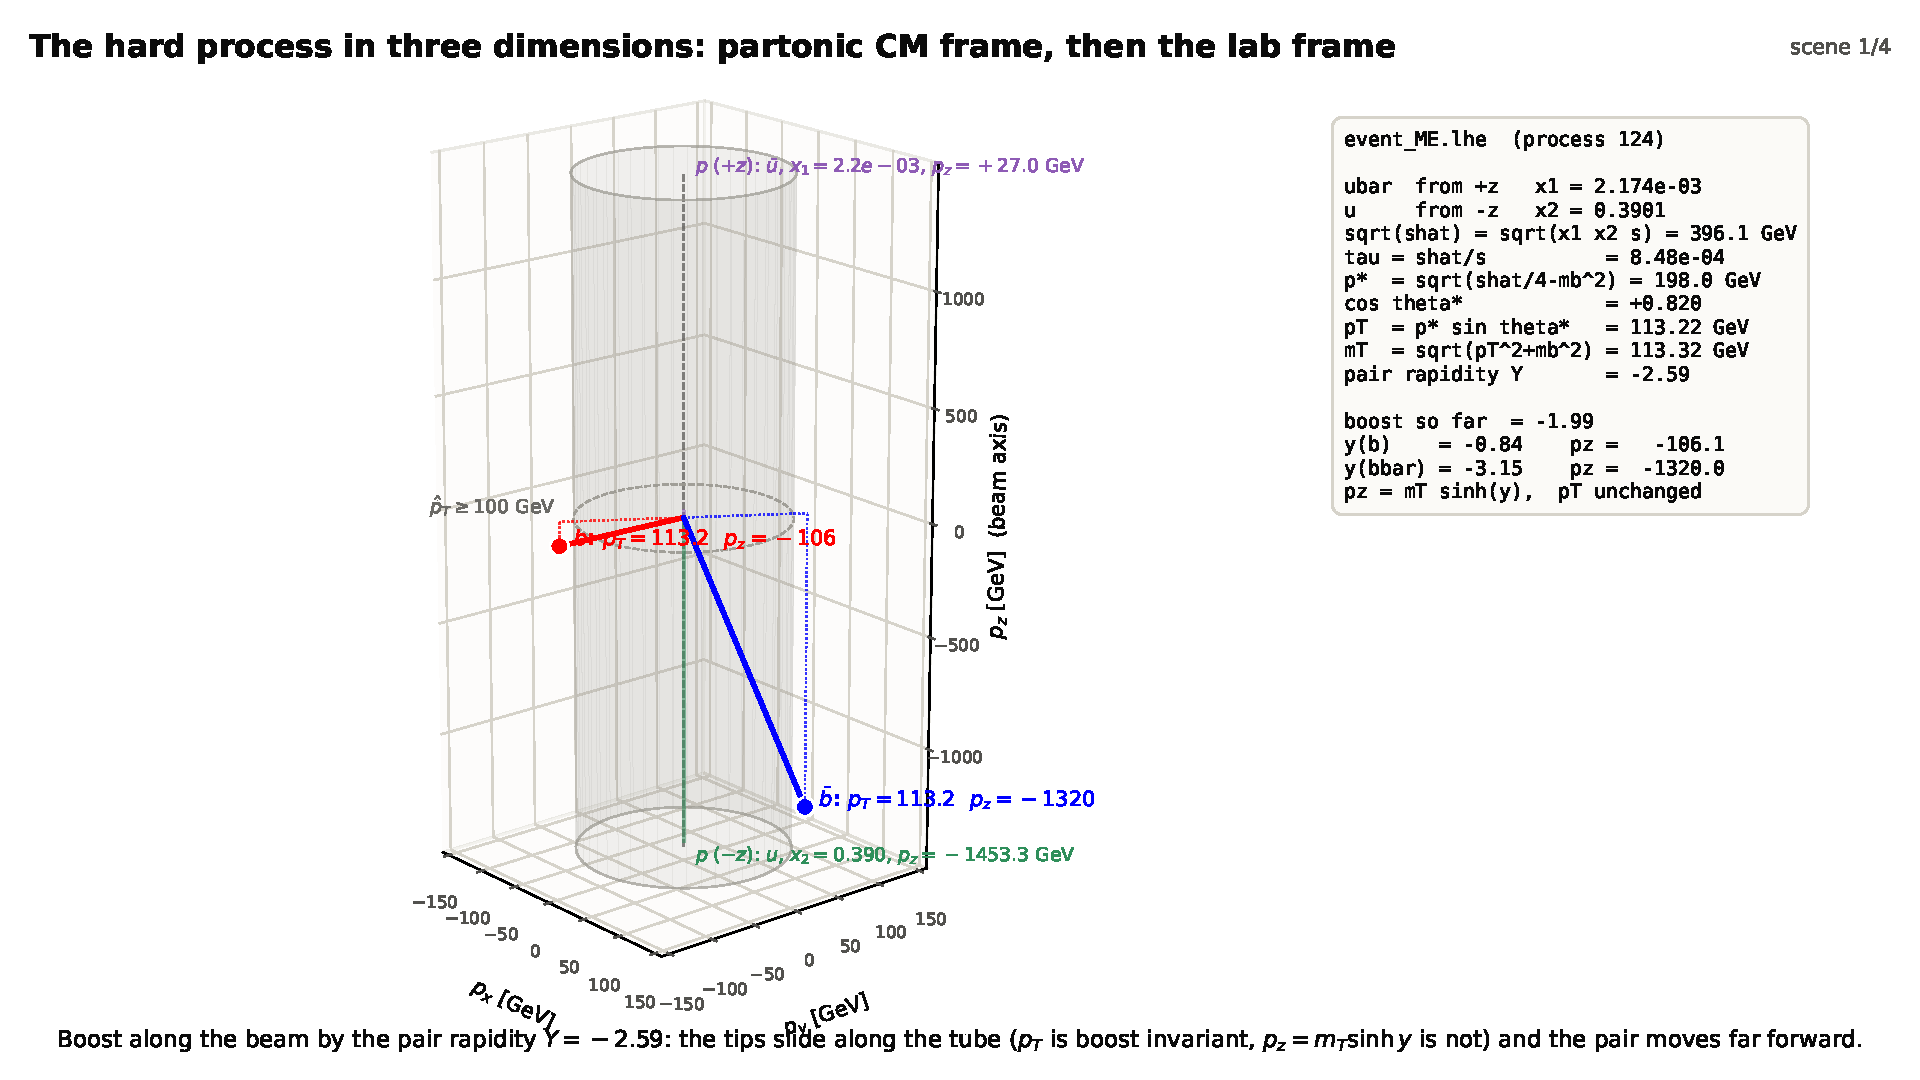
\includegraphics[page=1,width=0.47\textwidth]{ME/Standalone/animate_standalone_qqbar_bbbar_xsec_stills.pdf}\hfill
\includegraphics[page=2,width=0.47\textwidth]{ME/Standalone/animate_standalone_qqbar_bbbar_xsec_stills.pdf}\\[2mm]
\includegraphics[page=3,width=0.47\textwidth]{ME/Standalone/animate_standalone_qqbar_bbbar_xsec_stills.pdf}\hfill
\includegraphics[page=4,width=0.47\textwidth]{ME/Standalone/animate_standalone_qqbar_bbbar_xsec_stills.pdf}
\caption[Key frames of the animated standalone calculation]{Key frames of
the four scenes of the animated standalone calculation, drawn by
\file{animate_standalone_qqbar_bbbar_xsec.py} with \code{--stills}. Top left:
our event in the partonic frame with the $\pthat\ge100\GeV$ tube. Top right:
Sobol points morphed from the unit cube into
$(\log_{10}x_1,\log_{10}x_2,|\cos\theta|)$. Bottom left: the integrand over
the $(x_1,x_2)$ triangle, whose volume is the cross section. Bottom right:
the running average converging to $345\pb$. The film itself is the first of the
\jitjetworld playlist.}
\label{fig:ancestral_home:stills}
\end{figure}

\paragraph{The ancestral home in one picture.}
\Cref{fig:ancestral_home:factorisation_sketch} is the picture to carry from
this stop. Two protons approach along the beam; from each a single parton is
resolved, with a momentum fraction $x$ that the parton distribution function
assigns, and the two partons meet in the short-distance process we
calculate. The numbers on the sketch are those of our event: one parton with
two parts in a thousand of its proton's momentum, the other with
$39\%$, and a pair mass of $396\GeV$ out of the $13\,600\GeV$ the two protons
brought. Keep the asymmetry in mind; it decides where in the detector the
mother is born.

\begin{figure}[htbp]\centering
\resizebox{\textwidth}{!}{% ---------------------------------------------------------------------------
% The factorisation theorem as a picture: two protons, two parton densities,
% one short-distance blob. The x values, energies and the pair mass are those
% of our event (example/ME/event_ME.lhe) as listed in section [2] of the -v log
% of standalone_qqbar_bbbar_xsec.py. Input from chapter_01_ancestral_home.tex
% inside a figure environment.
% ---------------------------------------------------------------------------
\begin{tikzpicture}[x=1cm,y=1cm,
  every node/.style={font=\footnotesize},
  proton/.style={draw,ellipse,minimum width=22mm,minimum height=11mm,thick,fill=gray!10},
  valence/.style={thick,gray!70},
  fermion/.style={thick,postaction={decorate},decoration={markings,mark=at position 0.55 with {\arrow[scale=1.1]{Stealth}}}},
  antifermion/.style={thick,postaction={decorate},decoration={markings,mark=at position 0.45 with {\arrowreversed[scale=1.1]{Stealth}}}},
  remnant/.style={thick,gray!60,postaction={decorate},decoration={markings,mark=at position 0.6 with {\arrow[scale=0.9]{Stealth}}}},
  pdfblob/.style={draw,circle,minimum size=9mm,thick,fill=blue!12},
  hard/.style={draw,circle,minimum size=14mm,very thick,fill=orange!25},
  lab/.style={font=\scriptsize,align=center},
  num/.style={font=\scriptsize,align=center,text=blue!60!black},
  brace/.style={decorate,decoration={brace,amplitude=5pt},thick}]
% the two protons
\node[proton] (PA) at (-5.2,0) {};
\node[lab,above=1pt of PA] {proton A, $+z$, $P=6800\GeV$};
\node[proton] (PB) at (5.2,0) {};
\node[lab,above=1pt of PB] {proton B, $-z$, $P=6800\GeV$};
\foreach \dy in {-0.25,0,0.25} {\draw[valence] ($(PA.west)+(0.15,\dy)$) -- ($(PA.east)+(-0.15,\dy)$);
                                 \draw[valence] ($(PB.west)+(0.15,\dy)$) -- ($(PB.east)+(-0.15,\dy)$);}
% the PDF blobs
\node[pdfblob] (FA) at (-2.6,0) {$f_{\bar u}$};
\node[pdfblob] (FB) at (2.6,0) {$f_{u}$};
\draw[thick,gray!70] (PA.east) -- (FA.west);
\draw[thick,gray!70] (PB.west) -- (FB.east);
\node[lab,below=2pt of FA] {resolved at $\muF$};
\node[lab,below=2pt of FB] {resolved at $\muF$};
% remnants
\draw[remnant] (PA.east) -- (-3.4,-1.5) node[lab,below left=-2pt,text=gray!80!black] {remnant $(1-x_1)P$};
\draw[remnant] (PB.west) -- (3.4,-1.5) node[lab,below right=-2pt,text=gray!80!black] {remnant $(1-x_2)P$};
% the hard blob
\node[hard] (H) at (0,0) {$\hat\sigma$};
\draw[antifermion] (FA.east) -- (H.west);
\draw[fermion] (FB.west) -- (H.east);
\node[num,anchor=south] at (-1.7,0.42) {$\bar u$, $x_1P=14.8\GeV$\\$x_1=2.17\times10^{-3}$};
\node[num,anchor=south] at (1.85,0.42) {$u$, $x_2P=2653\GeV$\\$x_2=0.390$};
% outgoing b and bbar
\draw[fermion] (H.north east) -- (1.5,2.3) node[lab,right,text=red!80!black] {$b$: the mother, $\pt=113\GeV$};
\draw[antifermion] (H.south east) -- (1.5,-2.3) node[lab,right,text=blue!80!black] {$\bar b$, $\pt=113\GeV$};
\node[num,anchor=north east] at (-0.1,-0.9) {$\shat=x_1x_2s$\\$\sqrt{\shat}=396\GeV$};
% what is measured and what is calculated
\draw[brace] (-6.4,1.1) -- (-1.9,1.1) node[midway,above=6pt,lab] {long distance: \emph{measured once},\\the PDF $f_i(x_1,\muF^2)$};
\draw[brace] (1.9,1.1) -- (6.4,1.1) node[midway,above=6pt,lab] {long distance: \emph{measured once},\\the PDF $f_j(x_2,\muF^2)$};
\draw[brace] (0.8,2.75) -- (-0.8,2.75) node[midway,above=6pt,lab] {short distance: \emph{calculated},\\$\hat\sigma_{ij}(\shat;\muR^2,\muF^2)$};
% the sum over flavours and orientations
\node[lab,text=black!65,text width=12.5cm] at (0,-3.3) {$\sigma=\sum_{i,j}\int\!\mathrm{d}x_1\mathrm{d}x_2\,f_i(x_1)f_j(x_2)\,\hat\sigma_{ij}$:
  the sum runs over $d,u,s,c,b$ and both orientations ($q$ from A and $\bar q$ from B, and the reverse);
  our event is the $\bar u$-from-A, $u$-from-B term of the $u$ flavour.};
\end{tikzpicture}
}
\caption[The factorisation theorem as a picture]{The factorisation theorem as a picture. Two protons approach along the beam; from each a single parton is resolved at the scale $\muF$ with a momentum fraction $x$ given by the parton distribution function, and the two partons meet in the short-distance process $\hat\sigma$ that we calculate. The numbers are those of our event, from section~[2] of the \code{-v} log: $x_1=2.17\times10^{-3}$, $x_2=0.390$, $\sqrt{\shat}=396\GeV$. The remnants carry the rest of the two protons away and are forgotten until \cref{ch:whose_child}.}
\label{fig:ancestral_home:factorisation_sketch}
\end{figure}

\paragraph{The number, four ways.}
\label{sec:ancestral_home:validation}
\Cref{tab:ancestral_home:three_numbers} gives away the ending. The first
three rows are our own: a single Python file that needs only NumPy and SciPy
does the integral of \cref{sec:ancestral_home:theory} in about a second, a
sibling script does the same integral with LHAPDF and \PYTHIA's own coupling,
and the two agree to the fourth digit. The script has a learning mode,
\code{-v}, that narrates the calculation for our event factor by factor
before it runs it; every number quoted in the theory of this chapter is
taken from that log, so that you can put your finger on each one.
\label{sec:ancestral_home:standalone_code}\label{sec:ancestral_home:learning_mode}

The last two rows are the official packages. The CMS generator
configuration, one \code{GEN} step of the production chain, runs the same
process inside \PYTHIA, process code~124 with \code{HardQCD:qqbar2bbbar =
on}, the gluon channel off and \code{PhaseSpace:pTHatMin = 100}, and the
statistics table at the end of its log prints the cross section it sampled
from a thousand events: $3.486\times10^{-7}\,\mathrm{mb}$, that is
$348.6\pm6.0\pb$, half a standard deviation from our integral.
\label{sec:ancestral_home:cmssw}

\MG, a second generator that shares none of \PYTHIA's code, builds the one
Feynman diagram of $q\bar q\to\bbbar$ from a line typed at its prompt and
gives $344.3\pm1.0\pb$; its conventions differ in four known ways, a
four-flavour proton, a $b$ mass of $4.7\GeV$, its own dynamical scale and
the coupling of the PDF set, and \cref{sec:ancestral_home:scales} will put a
number on each.
\label{sec:ancestral_home:madgraph}

The agreement is the whole point of the stop: after this chapter you will
know what every knob in the CMS configuration does to the number, because
you will have turned each knob yourself. How each row was produced, the
commands to run, the configuration and the logs to read, is in the
companion of this chapter,
\begin{center}
  \companion{chapter_01_ME}
\end{center}
together with the full tables behind every number quoted below.

\begin{table}[htbp]\centering\small
\caption[The $q\bar q\to\bbbar$ cross section obtained four ways]{The
$q\bar q\to\bbbar$ cross section at $\sqrt{s}=13.6\TeV$ with
$\pthat\ge100\GeV$ obtained four ways. The first three rows use \PYTHIA's
conventions exactly ($\mb=4.8\GeV$, five incoming flavours, NNPDF3.1 NNLO,
$\muR^2=\muF^2=\pthat^2+\mb^2$, \PYTHIA's own $\alphas$ running); the \MG row
uses that program's defaults for the $b$ mass, the scale and the coupling,
and four incoming flavours (\cref{sec:ancestral_home:madgraph}). The scripts
are in \file{example/ME/Standalone/} and the generator inputs in
\file{example/ME/CMSSW/} and \file{example/ME/MadGraph/} of the JitJet
repository. Quoted errors are statistical or numerical only; the theoretical
uncertainty is the subject of \cref{sec:ancestral_home:scales}.}
\label{tab:ancestral_home:three_numbers}
\begin{tabular}{llr}\toprule
Method & Details & $\sigma$ [pb] \\ \midrule
Standalone script, one pass & LO integral, $2^{16}$ Sobol points & $345.320$ \\
Standalone script, 8 repeats & LO integral, scrambled seeds & $345.322 \pm 0.001$ \\
Full script (LHAPDF, \PYTHIA $\alphas$) & LO integral, 8 repeats & $345.324 \pm 0.001$ \\
\PYTHIA~8.311 in \code{CMSSW\_15\_0\_5} & Monte Carlo, 1000 events & $348.6 \pm 6.0$ \\
\MG~3.8.0 & Monte Carlo, 10\,000 events & $344.3 \pm 1.0$ \\
\bottomrule
\end{tabular}
\end{table}

\paragraph{Why $100\GeV$, and why this process.} A word about the route I
have chosen for us. The first draft of this journey used the more common
generator cut $\pthat\ge30\GeV$. With that cut the two $b$ quarks of our
event both flew off towards the endcaps, one of them into the forward
calorimeter where there is no tracker at all, and a passenger who wants to see
a $b$ jet being tagged would have waited in vain. Raising the cut to
$100\GeV$ costs a factor of fifty in rate, but it buys a mother born at
$|\eta|<1.5$, inside the barrel, where every subdetector of CMS will get a
look at her. Since we follow one event rather than measure a cross section,
that is the better bargain. And a word about the tools: the preface promises
that \MG generates Event~A. For this first stage we use \PYTHIA's own
$2\to2$ matrix element, because it is the process CMS actually runs in the
configuration of \cref{tab:ancestral_home:three_numbers}, and because its
leading-order matrix element is a formula short enough to check by hand. \MG
at leading order uses the very same Born matrix element, as
\cref{sec:ancestral_home:madgraph} shows.

\section{Let us dive into the details: the theory}
\label{sec:ancestral_home:theory}

\subsection{Two protons meet: the factorisation theorem in one page}
\label{sec:ancestral_home:two_protons_meet}

You have watched the number appear, and you have made it appear yourself.
Now we earn it. The next five subsections derive, factor by factor, the
integral that the script evaluates, end with the seven steps that its
\code{born\_weights} and \code{integrate} functions execute, and close with
an honest estimate of how much the result can be trusted.

Before any formula, a question to guess at. The two protons bring
$13\,600\GeV$ into the collision. How much of it did the hard process of our
event get to use? If your instinct says ``most of it'', look at the record in
\cref{sec:ancestral_home:our_jet}: the pair of $b$ quarks has a mass of
$396\GeV$, under three per cent of the beam energy, and one of the two
colliding partons carried only $15\GeV$. That is the normal case, not an
accident, and the reason is the subject of this section: a proton is not a
particle you can scatter, it is a bag of partons, each carrying a small and
random fraction of the momentum, and the formula below says how to add up
all the ways two of them can meet (\cref{fig:ancestral_home:factorisation_sketch}).

Look out of the left window: two protons are approaching each other at
$6800\GeV$ apiece. You cannot scatter a proton in perturbation theory; it is
a bound state, and the strong coupling inside it is not small. What rescues
us is the collinear factorisation theorem, which separates the problem into a
long-distance part that is measured once and for all, the parton
distribution functions (PDFs), and a short-distance part that we calculate,
the partonic cross section. For any inclusive hard process
$pp\to\bbbar+X$,
\begin{equation}
\begin{split}
  \sigma(pp\to\bbbar X) &= \sum_{i,j}\int_0^1\!\mathrm{d}x_1\int_0^1\!\mathrm{d}x_2\;
  f_i(x_1,\muF^2)\, f_j(x_2,\muF^2)\;
  \hat\sigma_{ij\to\bbbar}\!\left(\shat;\, \muR^2,\muF^2\right) \\
  &\quad + \mathcal{O}\!\left(\frac{\Lambda^2_{\mathrm{QCD}}}{\pthat^2}\right),
  \qquad \shat = x_1x_2 s .
\end{split}
  \label{eq:ancestral_home:factorisation}
\end{equation}
Read it slowly; it is the most important equation of the chapter. Here
$f_i(x,\muF^2)\,\mathrm{d}x$ is the number of partons of flavour $i$ carrying
a fraction between $x$ and $x+\mathrm{d}x$ of the proton momentum, resolved at
the factorisation scale $\muF$; $\hat\sigma_{ij}$ is the cross section for
the two partons, computed in perturbation theory with the strong coupling
evaluated at the renormalisation scale $\muR$; and $\shat$ is the squared
centre-of-mass energy of the two partons, the only energy the hard scattering
knows about. The two protons are identical, so the sum over $(i,j)$ counts
both a $q$ from beam~1 meeting a $\bar q$ from beam~2 and the reverse. Forget
one orientation and you lose half the cross section; it is the first thing to
check in any integrator.

\paragraph{The numbers.} Section~[2] of the log evaluates the formula at
our event. The $\bar u$ from beam~A carries $x_1=2.174\times10^{-3}$ and the
$u$ from beam~B $x_2=0.3901$, so $\shat=x_1x_2s=156\,895\GeV^2$ and
$\sqrt{\shat}=396.1\GeV$, the mass that the record prints as its momentum
sum. The two orientations of the sum are far from equal at this one point:
the $\bar u$-from-A, $u$-from-B term is $470.2\pb$ of the $u$-flavour weight
and the reverse term $3.0\pb$, because a $u$ quark with $x=2\times10^{-3}$
is common and a $\bar u$ with $x=0.39$ is rare. Integrated over the whole
phase space the two orientations contribute exactly equally, by the symmetry
of the two beams, which is why forgetting one costs a factor of two and not
some odd fraction. \Cref{fig:ancestral_home:factorisation_plot} shows the
same integrand over all of phase space: the rate is concentrated just above
the threshold, $63\%$ of it below $\sqrt{\shat}=305\GeV$, and spread over
five units of pair rapidity; our event, at $396\GeV$ and $Y=-2.59$, sits on
the slope of both distributions, and only $9\%$ of all pairs are boosted
even more than ours.

\begin{figure}[htbp]\centering
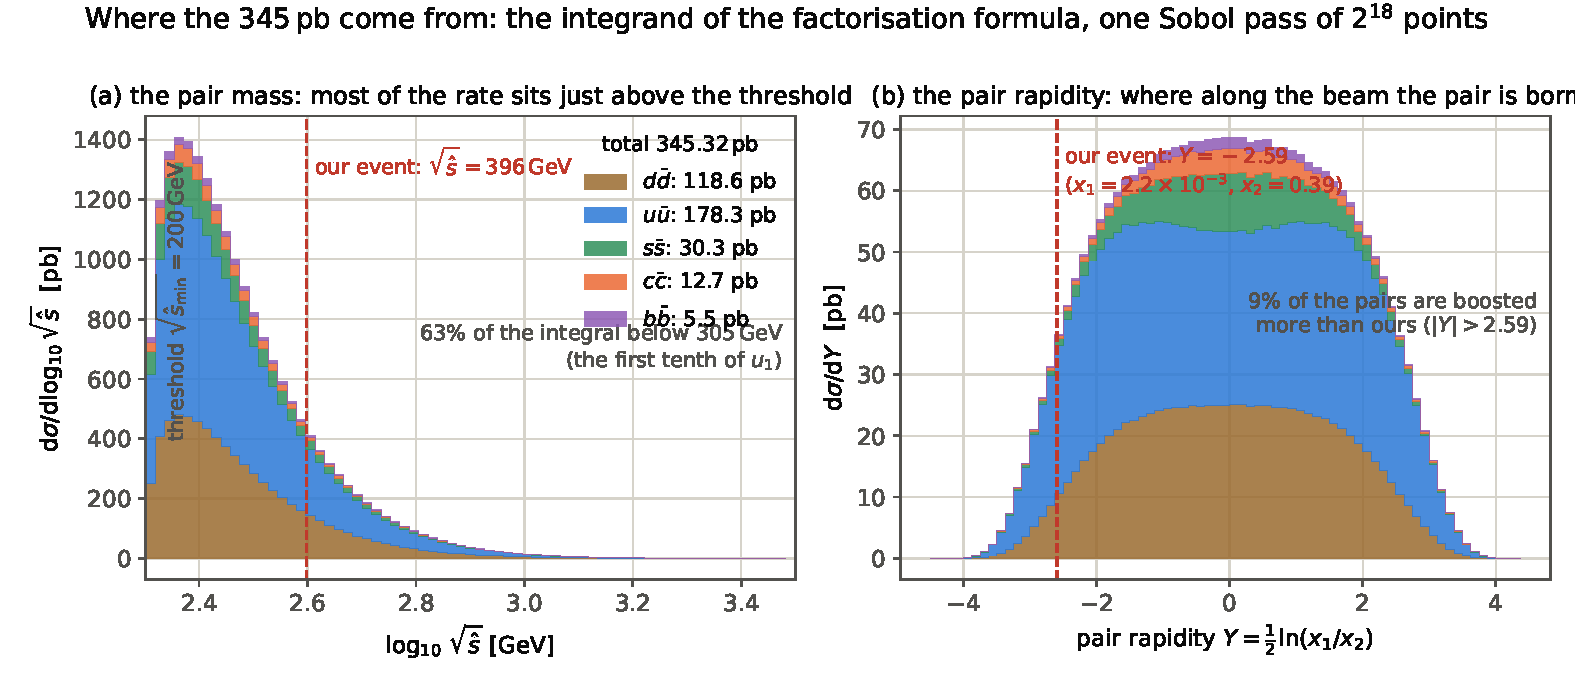
\includegraphics[page=1,width=\textwidth]{ME/Standalone/theory_qqbar_bbbar.pdf}
\caption[The integrand of the factorisation formula over the phase space]{The integrand of the factorisation formula, from one Sobol pass of $2^{18}$ points of \file{plot_theory_ME.py}, split by incoming flavour. (a) The distribution in the pair mass $\sqrt{\shat}$: the PDFs rise towards small $x$ and $\hat\sigma\propto1/\shat$, so most of the rate sits just above the threshold $\sqrt{\shat_{\min}}=200\GeV$ set by the $\pthat$ cut. (b) The distribution in the pair rapidity $Y$: flat where both $x$ are small, falling where one parton has to be a valence quark at large $x$. Our event is the dashed line in both panels.}
\label{fig:ancestral_home:factorisation_plot}
\end{figure}

\subsubsection{Better variables, and a Jacobian you should do once by hand}
\label{sec:ancestral_home:better_variables}

The integral over $x_1$ and $x_2$ is awkward: the PDFs rise steeply towards
small $x$, and the physics depends on the two fractions mostly through their
product. For a $2\to2$ process the natural variables are the pair's
squared-mass fraction and rapidity,
\begin{equation}
  \tau \equiv x_1x_2 = \frac{\shat}{s},\qquad
  Y \equiv \tfrac12\ln\frac{x_1}{x_2},\qquad
  x_{1} = \sqrt{\tau}\,e^{+Y},\quad x_{2} = \sqrt{\tau}\,e^{-Y}.
  \label{eq:ancestral_home:tauY}
\end{equation}
Check the inverse yourself: $x_1x_2=\tau$ and
$\tfrac12\ln(x_1/x_2)=\tfrac12\ln e^{2Y}=Y$. $Y$ is the rapidity of the
$\bbbar$ pair in the laboratory, and it will turn out to be the single number
that decides where in the detector our mother is born.

\begin{figure}[htbp]\centering
\resizebox{\textwidth}{!}{% ---------------------------------------------------------------------------
% The change of variables (x1, x2) -> (ln tau, Y): the allowed triangle, the
% lines of constant tau and Y, and the little rectangle whose image has area
% tau d ln tau dY. Numbers (tau_min, our event) from section [1] and [2] of the
% -v log of standalone_qqbar_bbbar_xsec.py.
% ---------------------------------------------------------------------------
\begin{tikzpicture}[x=1cm,y=1cm,
  every node/.style={font=\footnotesize},
  axis/.style={-{Stealth},thick},
  iso/.style={gray!60,thin},
  lab/.style={font=\scriptsize,align=center},
  head/.style={font=\small\bfseries},
  ev/.style={star,star points=5,star point ratio=2.2,fill=red!80!black,draw=white,inner sep=0pt,minimum size=3.2mm},
  bigarrow/.style={-{Stealth[length=3mm,width=3mm]},gray!60,line width=2.4pt}]
% ---------------- (a) the (ln x1, ln x2) plane: a triangle ---------------------------------
% horizontal: -ln x1 (x1 decreases to the right), vertical: -ln x2; origin = the tau = 1 corner
\begin{scope}
\node[head,anchor=west] at (-0.2,4.9) {(a) the $(\ln x_1,\ln x_2)$ plane};
\fill[blue!8] (0,0) -- (4.2,0) -- (0,4.2) -- cycle;
\draw[axis] (-0.3,0) -- (4.9,0) node[below left] {$-\ln x_1$};
\draw[axis] (0,-0.3) -- (0,4.9) node[below left] {$-\ln x_2$};
\node[lab,anchor=north] at (4.2,-0.1) {$x_1=\tau_{\min}$};
\node[lab,anchor=east] at (-0.1,4.2) {$x_2=\tau_{\min}$};
\node[lab,anchor=north east] at (-0.05,-0.05) {$x_1=x_2=1$\\$(\tau=1)$};
\draw[thick] (4.2,0) -- (0,4.2);
\node[lab,rotate=-45] at (2.6,2.0) {$x_1x_2=\tau_{\min}=2.17\times10^{-4}$};
\foreach \t in {1.4,2.8} {\draw[iso] (\t,0) -- (0,\t);}
\node[lab,rotate=-45,text=gray!80!black] at (1.75,1.75) {$\tau=\mathrm{const}$};
\draw[iso,dashed] (0,0) -- (2.1,2.1);
\draw[iso,dashed] (1.4,0) -- (2.8,1.4);
\draw[iso,dashed] (0,1.4) -- (1.4,2.8);
\node[lab,rotate=45,text=gray!80!black] at (1.3,1.55) {$Y=0$};
\node[lab,rotate=45,text=gray!80!black] at (2.15,0.95) {$Y<0$};
\node[lab,rotate=45,text=gray!80!black] at (0.75,2.35) {$Y>0$};
\node[ev] at (3.05,0.47) {};
\node[lab,anchor=east,text=red!80!black] at (2.9,0.5) {our event, $Y=-2.59$};
\node[lab,text=black!65,text width=4.6cm,anchor=north west] at (-0.2,-0.95) {The region above the threshold line is a triangle: $\tau$ is constant along the anti-diagonals, $Y$ along the diagonals ($Y<0$: $x_1<x_2$, our side).};
\end{scope}
\draw[bigarrow] (5.3,2.2) -- (6.1,2.2);
% ---------------- (b) the (ln tau, Y) plane ---------------------------------------------------
\begin{scope}[xshift=7.2cm]
\node[head,anchor=west] at (-0.2,4.9) {(b) the $(\ln\tau,Y)$ plane};
\fill[blue!8] (0,2.2) -- (4.2,4.3) -- (4.2,0.1) -- cycle;
\draw[axis] (-0.3,2.2) -- (4.9,2.2) node[below left] {$\ln\tau$};
\draw[axis] (0,-0.3) -- (0,4.9) node[below left] {$Y$};
\node[lab,anchor=north] at (0,2.1) {$\ln\tau_{\min}$};
\node[lab,anchor=north] at (4.2,2.1) {$0$};
\draw[thick] (0,2.2) -- (4.2,4.3) node[lab,pos=0.55,above,sloped] {$Y_{\max}=-\tfrac12\ln\tau$};
\draw[thick] (0,2.2) -- (4.2,0.1) node[lab,pos=0.88,below,sloped] {$-Y_{\max}$};
\foreach \t in {1.4,2.8} {\draw[iso] (\t,{2.2-(4.2-\t)/2}) -- (\t,{2.2+(4.2-\t)/2});}
\foreach \y in {1.5,2.9} {\draw[iso,dashed] ({4.2-2*abs(\y-2.2)},\y) -- (4.2,\y);}
\draw[iso,dashed] (0,2.2) -- (4.2,2.2);
% the little rectangle
\fill[orange!60] (1.55,1.5) rectangle (1.95,1.9);
\draw[thick,orange!80!black] (1.55,1.5) rectangle (1.95,1.9);
\node[lab,anchor=south west,text=orange!80!black] at (1.9,1.9) {$\mathrm{d}\ln\tau\,\mathrm{d}Y$};
\node[ev] at (0.68,0.95) {};
\draw[red!80!black,thin] (0.68,0.95) -- (1.6,-0.15);
\node[lab,anchor=north,text=red!80!black] at (1.9,-0.15) {our event: $\ln\tau=-7.07$, $Y=-2.59$ ($73\%$ of $Y_{\max}=3.54$)};
\node[lab,text=black!65,text width=4.6cm,anchor=north west] at (-0.2,-1.15) {The unit cube is mapped linearly onto this triangle: $u_1$ along $\ln\tau$ over the length $\ln(1/\tau_{\min})=8.44$, $u_2$ along $Y$ over $2Y_{\max}(\tau)$.};
\end{scope}
\draw[bigarrow] (12.5,2.2) -- (13.3,2.2);
% ---------------- (c) the Jacobian in the linear (x1, x2) plane --------------------------------
\begin{scope}[xshift=14.4cm]
\node[head,anchor=west] at (-0.2,4.9) {(c) the Jacobian, $\mathrm{d}x_1\mathrm{d}x_2=\tau\,\mathrm{d}\ln\tau\,\mathrm{d}Y$};
\draw[axis] (-0.3,0) -- (4.9,0) node[below left] {$x_1$};
\draw[axis] (0,-0.3) -- (0,4.9) node[below left] {$x_2$};
% a hyperbola tau = const and its neighbour
\draw[iso] plot[domain=0.5:4.3,samples=60] (\x,{2.0/\x});
\draw[iso] plot[domain=0.62:4.3,samples=60] (\x,{2.6/\x});
\node[lab,text=gray!80!black,anchor=west] at (3.4,0.95) {$\tau$ and $\tau e^{\mathrm{d}\ln\tau}$};
% rays Y = const and neighbour
\draw[iso,dashed] (0,0) -- (3.9,3.9);
\draw[iso,dashed] (0,0) -- (4.3,2.9);
\node[lab,text=gray!80!black,anchor=west,rotate=34] at (3.2,2.15) {$Y$ and $Y+\mathrm{d}Y$};
% the parallelogram: corners at the intersections
\coordinate (p1) at (1.414,1.414); \coordinate (p2) at (1.612,1.612);
\coordinate (p3) at (1.964,1.324); \coordinate (p4) at (1.723,1.161);
\fill[orange!60] (p1) -- (p2) -- (p3) -- (p4) -- cycle;
\draw[thick,orange!80!black] (p1) -- (p2) -- (p3) -- (p4) -- cycle;
\node[lab,anchor=south west,text=orange!80!black] at (2.0,1.55) {area $=\tau\,\mathrm{d}\ln\tau\,\mathrm{d}Y$};
\node[lab,text=black!65,text width=4.6cm,anchor=north west] at (-0.2,-0.95) {The rectangle becomes a tilted parallelogram $\tau$ times larger. Since the libraries return $xf$, the two factors of $\tau$ cancel: at our event $f_{\bar u}f_u\,\tau=0.2413=[x_1f_{\bar u}][x_2f_u]$.};
\end{scope}
\end{tikzpicture}
}
\caption[The change of variables from $(x_1,x_2)$ to $(\ln\tau,Y)$]{The change of variables from $(x_1,x_2)$ to $(\ln\tau,Y)$. (a) In the $(\ln x_1,\ln x_2)$ plane the allowed region is a triangle bounded by $x_1x_2=\tau_{\min}$; $\tau$ is constant along one diagonal direction and $Y$ along the other. (b) In the $(\ln\tau,Y)$ plane the same region is the triangle $|Y|\le-\tfrac12\ln\tau$, onto which the unit square of $(u_1,u_2)$ is mapped linearly. (c) A small rectangle $\mathrm{d}\ln\tau\,\mathrm{d}Y$ becomes a parallelogram of area $\tau\,\mathrm{d}\ln\tau\,\mathrm{d}Y$ in the linear $(x_1,x_2)$ plane: the Jacobian of \cref{eq:ancestral_home:jacobian}. Our event is marked with the numbers of section~[2] of the log.}
\label{fig:ancestral_home:jacobian_sketch}
\end{figure}

Now the part I would like you to do once with pencil and paper, because
every Monte Carlo integrator you will ever meet hides it. When we change
variables from $(x_1,x_2)$ to $(\ln\tau,Y)$ the little area element
$\mathrm{d}x_1\,\mathrm{d}x_2$ is stretched, and the Jacobian says by how
much. Write $x_1=e^{\frac12\ln\tau+Y}$ and $x_2=e^{\frac12\ln\tau-Y}$ and
differentiate:
\begin{equation}
  \frac{\partial x_1}{\partial\ln\tau}=\tfrac12x_1,\quad
  \frac{\partial x_1}{\partial Y}=x_1,\qquad
  \frac{\partial x_2}{\partial\ln\tau}=\tfrac12x_2,\quad
  \frac{\partial x_2}{\partial Y}=-x_2 .
\end{equation}
The Jacobian matrix and its determinant are
\begin{equation}
  J=\begin{pmatrix}\tfrac12x_1 & x_1\\[2pt] \tfrac12x_2 & -x_2\end{pmatrix},
  \qquad
  \det J=\left(\tfrac12x_1\right)(-x_2)-x_1\left(\tfrac12x_2\right)=-x_1x_2=-\tau,
\end{equation}
so that
\begin{equation}
  \mathrm{d}x_1\,\mathrm{d}x_2=\tau\,\mathrm{d}\ln\tau\,\mathrm{d}Y .
  \label{eq:ancestral_home:jacobian}
\end{equation}
Picture a tiny rectangle in the $(\ln\tau,Y)$ plane; in the $(x_1,x_2)$
plane it becomes a tilted parallelogram of area $\tau$ times the original.
Nothing deep, but now comes the payoff. PDF libraries do not return $f(x)$;
they return $x f(x,Q^2)$, because that is the quantity of order one across
the whole $x$ range. Multiply and divide by $x_1x_2=\tau$:
\begin{equation}
  f_i(x_1)f_j(x_2)\,\mathrm{d}x_1\mathrm{d}x_2
  = \frac{[x_1f_i(x_1)]\,[x_2f_j(x_2)]}{\tau}\;\tau\,\mathrm{d}\ln\tau\,\mathrm{d}Y
  = [x_1f_i(x_1)]\,[x_2f_j(x_2)]\;\mathrm{d}\ln\tau\,\mathrm{d}Y .
  \label{eq:ancestral_home:xf}
\end{equation}
The two factors of $\tau$ cancel exactly. That is why every integrator in this
chapter samples $\ln\tau$ and $Y$, multiplies the two $xf$ values it gets
from the library, and never divides by $x$. If you ever see a stray factor
$x_1x_2$ in such a code, this is where it came from. The limits are
$\tau_{\min}\le\tau\le1$, with $\tau_{\min}$ fixed by the kinematic cut
(\cref{sec:ancestral_home:matrix_element}), and
\begin{equation}
  |Y|\le Y_{\max}(\tau)\equiv-\tfrac12\ln\tau ,
  \label{eq:ancestral_home:ymax}
\end{equation}
which is simply the statement that both $x_1=\sqrt\tau e^{Y}$ and
$x_2=\sqrt\tau e^{-Y}$ must stay below one. The allowed region in the
$(\ln x_1,\ln x_2)$ plane is a triangle, and you have seen it drawn in
scene~2 of the film (\cref{fig:ancestral_home:stills}). \Cref{app:kinematics} collects these
variables together with the rest of the kinematic vocabulary of the book.

\paragraph{The numbers.} At our event the log gives $\tau=8.483\times10^{-4}$,
$\ln\tau=-7.072$ and $Y=-2.595$; the rapidity range allowed at this $\tau$ is
$|Y|\le Y_{\max}=3.536$, of which our pair uses $73\%$, and the constants of
section~[1] are $\tau_{\min}=2.168\times10^{-4}$ and $\ln(1/\tau_{\min})=8.437$,
the length of the $\ln\tau$ interval. The cancellation of
\cref{eq:ancestral_home:xf} is checked explicitly: the library values are
$x_1f_{\bar u}=1.1455$ and $x_2f_u=0.2107$, the densities themselves are
$f_{\bar u}(x_1)=526.8$ and $f_u(x_2)=0.540$, and
$f_{\bar u}f_u\,\tau=0.24133=[x_1f_{\bar u}][x_2f_u]$ to five digits. The
reason for sampling $\ln\tau$ rather than $\tau$ is in
\cref{fig:ancestral_home:variables_plot}: with the logarithmic map the first
of $24$ bins in $u_1$ carries $26\%$ of the integral and the rest fall off
smoothly, which an integrator can handle; with a linear map in $\tau$ the
first bin would carry more than $99.99\%$, and $96\%$ of the points would be
spent where there is nothing to integrate.

\begin{figure}[htbp]\centering
\includegraphics[page=2,width=\textwidth]{ME/Standalone/theory_qqbar_bbbar.pdf}
\caption[The allowed triangle and the choice of $\ln\tau$ as integration variable]{The change of variables at work, from \file{plot_theory_ME.py}. (a) The integrand $\mathrm{d}^2\sigma/\mathrm{d}\log_{10}x_1\,\mathrm{d}\log_{10}x_2$ over the allowed triangle, with lines of constant $\tau$ and constant $Y$ and our event marked; the colour scale spans five orders of magnitude. (b) The fraction of the integral in each of $24$ bins of $u_1$ when $\ln\tau$ is sampled, as the script does. (c) The same fraction in bins of a coordinate linear in $\tau$: essentially all of the integral falls in the first bin, and a uniform sample would waste almost every point.}
\label{fig:ancestral_home:variables_plot}
\end{figure}

\subsection{Parton distribution functions: where the mother comes from}
\label{sec:ancestral_home:pdfs}

A question before the formula. A proton is two $u$ quarks and a $d$ quark;
where, then, did the $\bar u$ antiquark of our event come from, and how
likely was it that a proton contained one with a momentum fraction of two
parts in a thousand? Guess a number, then look at the second row of
\cref{tab:ancestral_home:pdf_values}: $x_1f_{\bar u}=1.15$, an antiquark
density \emph{larger} than the valence density $x_2f_u=0.21$ that the $u$
quark of beam~B came with. At small $x$ a proton is mostly gluons and
quark--antiquark pairs that the gluons have split into, and the three valence
quarks are a minority (\cref{fig:ancestral_home:proton_sketch}). The parton
distribution function is the bookkeeping of this crowd.

\begin{figure}[htbp]\centering
\resizebox{\textwidth}{!}{% ---------------------------------------------------------------------------
% What a PDF describes: the proton seen at a resolution mu_F, with the valence
% quarks, the gluons and the sea; our two incoming partons marked with their
% x and xf values (section [2] of the -v log). Panel (b): raising mu_F resolves
% more of the sea and softens the valence, the mechanism behind the mu_F rows.
% ---------------------------------------------------------------------------
\begin{tikzpicture}[x=1cm,y=1cm,
  every node/.style={font=\footnotesize},
  proton/.style={draw,circle,very thick,fill=gray!8},
  val/.style={circle,fill=blue!70!black,inner sep=0pt,minimum size=3.2mm,text=white,font=\tiny},
  sea/.style={circle,fill=violet!70,inner sep=0pt,minimum size=1.8mm},
  seabar/.style={circle,draw=violet!70,thick,fill=white,inner sep=0pt,minimum size=1.8mm},
  gluon/.style={thick,decorate,decoration={coil,aspect=0,segment length=3pt,amplitude=1.3pt},gray!70},
  lab/.style={font=\scriptsize,align=center},
  head/.style={font=\small\bfseries},
  bigarrow/.style={-{Stealth[length=3mm,width=3mm]},gray!60,line width=2.4pt}]
% ---------------- (a) the proton at the scale mu_F = 113 GeV -------------------------------------
\node[head,anchor=west] at (-2.9,3.4) {(a) a proton resolved at $\muF=113\GeV$};
\node[proton,minimum size=52mm] (P) at (0,0) {};
\node[val] (u1) at (-0.9,0.7) {$u$};
\node[val] (u2) at (1.0,0.4) {$u$};
\node[val] (d1) at (0.1,-1.0) {$d$};
\draw[gluon] (u1) -- (u2);
\draw[gluon] (u2) -- (d1);
\draw[gluon] (d1) -- (u1);
\draw[gluon] (u1) -- (-1.9,1.3);
\draw[gluon] (u2) -- (1.9,-0.4);
\draw[gluon] (d1) -- (-0.5,-2.0);
\foreach \px/\py/\qx/\qy in {-1.7/-0.2/-1.45/-0.45,1.5/1.4/1.75/1.15,-0.3/1.9/0.0/1.75,1.2/-1.6/1.45/-1.4,-1.9/1.3/-2.1/1.0,0.7/-2.1/0.45/-2.25}
  {\node[sea] at (\px,\py) {}; \node[seabar] at (\qx,\qy) {};}
\node[lab,anchor=west] at (3.0,2.0) {\tikz\node[val,minimum size=2.6mm]{};\; valence quark: $x\sim0.1$--$0.5$, the proton's identity};
\node[lab,anchor=west] at (3.0,1.3) {\tikz\draw[gluon] (0,0)--(0.6,0);\; gluon: half the momentum, dominant at small $x$};
\node[lab,anchor=west] at (3.0,0.6) {\tikz{\node[sea]{};\node[seabar] at (0.25,0){};}\; sea pair from $g\to q\bar q$: $x\lesssim10^{-2}$, $xf\sim1$};
% our two partons
\draw[-{Stealth},thick,red!70!black] (3.0,-0.5) -- (1.25,0.3);
\node[lab,anchor=west,text=red!70!black] at (3.0,-0.5) {our $u$ (beam B): valence, $x_2=0.390$,\\$x_2f_u=0.2107$, on the broad bump};
\draw[-{Stealth},thick,violet] (3.0,-1.6) -- (-1.3,-0.45);
\node[lab,anchor=west,text=violet] at (3.0,-1.6) {our $\bar u$ (beam A): sea, $x_1=2.17\times10^{-3}$,\\$x_1f_{\bar u}=1.1455$, where $xf$ is of order one};
\node[lab,text=black!65,text width=6.8cm,anchor=north west] at (3.0,-2.3) {$f_i(x,\muF^2)\,\mathrm{d}x$ counts the partons of flavour $i$ with momentum fraction in $[x,x+\mathrm{d}x]$ when the proton is probed at the scale $\muF$. The picture is a snapshot; the numbers are a fit to data.};
% ---------------- (b) the same proton at two resolutions ------------------------------------------
\begin{scope}[xshift=13.4cm]
\node[head,anchor=west] at (-1.4,3.4) {(b) resolution: raising $\muF$ resolves more sea};
\node[proton,minimum size=22mm] (Q1) at (0,1.2) {};
\node[val,minimum size=2.6mm] at (-0.35,1.45) {}; \node[val,minimum size=2.6mm] at (0.4,1.35) {}; \node[val,minimum size=2.6mm] at (0.0,0.75) {};
\node[sea,minimum size=1.5mm] at (-0.6,0.8) {}; \node[seabar,minimum size=1.5mm] at (-0.45,0.65) {};
\node[lab,anchor=west] at (1.3,1.2) {$\muF=57\GeV$ ($Q^2/4$):\\fewer sea quarks, harder valence\\$x_1f_{\bar u}$ lower by $9\%$, $x_2f_u$ higher by $10\%$};
\node[proton,minimum size=22mm] (Q2) at (0,-1.5) {};
\node[val,minimum size=2.6mm] at (-0.35,-1.25) {}; \node[val,minimum size=2.6mm] at (0.4,-1.35) {}; \node[val,minimum size=2.6mm] at (0.0,-1.95) {};
\foreach \px/\py/\qx/\qy in {-0.6/-1.9/-0.45/-2.05,0.6/-0.9/0.75/-1.05,-0.7/-1.1/-0.85/-1.25,0.3/-2.2/0.45/-2.05}
  {\node[sea,minimum size=1.5mm] at (\px,\py) {}; \node[seabar,minimum size=1.5mm] at (\qx,\qy) {};}
\node[lab,anchor=west] at (1.3,-1.5) {$\muF=227\GeV$ ($4Q^2$):\\more sea quarks, softer valence\\$x_1f_{\bar u}$ higher by $8\%$, $x_2f_u$ lower by $9\%$};
\draw[bigarrow] (0,0.0) -- (0,-0.3);
\node[lab,text=black!65,text width=6.6cm,anchor=north west] at (-1.4,-2.9) {DGLAP evolution: the gluon feeds the sea as $Q^2$ grows and the valence quarks lose momentum to radiation. This is why $\muF$ pulls the two PDF factors of our event in opposite directions (\cref{tab:ancestral_home:variations}).};
\end{scope}
\end{tikzpicture}
}
\caption[What a parton distribution function describes]{What a parton distribution function describes. (a) A proton resolved at the scale $\muF=113\GeV$ of our event: three valence quarks, the gluons that bind them and a sea of quark--antiquark pairs from gluon splitting. The $u$ of beam~B is a valence quark at $x_2=0.39$, the $\bar u$ of beam~A a sea antiquark at $x_1=2.2\times10^{-3}$, where $xf$ is of order one. (b) The same proton resolved at half and at twice the scale: raising $\muF$ resolves more of the sea and softens the valence quarks, the DGLAP evolution of \cref{eq:ancestral_home:dglap}. The percentages are those of section~[2] of the \code{-v} log.}
\label{fig:ancestral_home:proton_sketch}
\end{figure}

The PDFs cannot be computed from first principles; they are fitted to data
and evolved in $Q^2$ with the DGLAP equations. CMS Run~3 simulation uses the
NNPDF3.1 NNLO set with $\alphas(m_Z)=0.118$~\cite{NNPDF:2017mvq}, member~0
(the central replica), accessed through LHAPDF~\cite{Buckley:2014ana} under the
name \code{NNPDF31\_nnlo\_as\_0118} and the numeric ID~303600. The set is
distributed as a table of $x f(x,Q^2)$ on a grid of knots in $x$ and $Q$;
LHAPDF interpolates between the knots with cubic splines in $(\ln x,\ln Q^2)$.

\paragraph{The equations.} Three statements define what the table means.
First the definition itself: $f_i(x,\muF^2)\,\mathrm{d}x$ is the number of
partons of flavour $i$ with momentum fraction in $[x,x+\mathrm{d}x]$ when the
proton is probed at the resolution $\muF$. Second the sum rules that pin the
normalisation,
\begin{equation}
  \int_0^1\!\mathrm{d}x\,\bigl[u(x)-\bar u(x)\bigr]=2,\qquad
  \int_0^1\!\mathrm{d}x\,\bigl[d(x)-\bar d(x)\bigr]=1,\qquad
  \sum_i\int_0^1\!\mathrm{d}x\;x f_i(x,\muF^2)=1 ,
  \label{eq:ancestral_home:sumrules}
\end{equation}
which say that the proton has two valence $u$ quarks and one valence $d$
whatever the scale, and that the partons together carry all of its momentum;
the gluon, absent from our process, takes about half. Third the DGLAP
evolution equation, which is the only part of a PDF that perturbation theory
predicts: the dependence on the scale,
\begin{equation}
  \muF^2\,\frac{\partial f_i(x,\muF^2)}{\partial\muF^2}
  =\frac{\alphas(\muF^2)}{2\pi}\sum_j\int_x^1\frac{\mathrm{d}z}{z}\,
  P_{ij}(z)\,f_j\!\left(\frac{x}{z},\muF^2\right).
  \label{eq:ancestral_home:dglap}
\end{equation}
Read it as a flow: when the resolution is raised, a parton $j$ at $x/z$ is
seen to split into a parton $i$ that keeps the fraction $z$ of its momentum,
with the probability $P_{ij}(z)$. The splitting function $P_{qg}$ feeds the
sea from the gluon, so sea densities at small $x$ \emph{rise} with $\muF$;
the function $P_{qq}$ moves a valence quark to smaller $x$ by radiating a
gluon, so the valence density at large $x$ \emph{falls}. Both signs will
matter for us. The $P_{ij}$ themselves are the splitting functions of the
parton shower, and \cref{ch:mother_gives_birth} derives them; here they
are the fit's evolution kernel and the data fix the rest.

Three conventions of the interface matter for reproducing \PYTHIA's numbers,
and you would not guess any of them from the physics:
\begin{itemize}[nosep]
  \item \textbf{Freezing at the grid edges.} Outside the tabulated range in
    $x$ or $Q^2$ the value at the nearest edge is used rather than an
    extrapolation.
  \item \textbf{Clipping.} Fitted PDFs can go slightly negative at large $x$
    and for heavy flavours; \PYTHIA's proton wrapper sets such values to zero.
    In the default integration $1.4$ million of the individual PDF evaluations
    were clipped, yet the effect on the cross section is $0.08\%$
    (\cref{tab:ancestral_home:variations}), because the clipped values are tiny.
  \item \textbf{Symmetric heavy sea.} The charm and bottom antiquark
    densities are taken equal to the quark densities, $\bar c=c$ and
    $\bar b=b$, as in the wrapper.
\end{itemize}

\paragraph{Our event.} Now look at the record of the event we follow through
this book (\cref{sec:ancestral_home:our_jet}). The mother was produced by an
antiquark from beam~A and a quark from beam~B, and the two partons could
hardly be more different. The $\bar u$ carries $x_1=2.17\times10^{-3}$ of its
proton: it is a sea antiquark, drawn from the rising small-$x$ region where
$xf$ is of order one. The $u$ carries $x_2=0.390$: a valence quark, right on
the broad bump of the valence distribution. \Cref{tab:ancestral_home:pdf_values}
gives the values. The asymmetry is the first fact about our mother's birth.
The pair is boosted along the beam with rapidity
$Y=\tfrac12\ln(x_1/x_2)=-2.59$, so both $b$ quarks emerge backward, and the
mother we follow is born at $\eta=-1.44$, comfortably inside the barrel. In
the $30\GeV$ draft the same asymmetry was even stronger ($x_1=2.8\times10^{-4}$,
$Y=-3.47$) and pushed her to the edge of the tracker; the higher cut forces a
larger $\shat=\tau s$, hence a larger $x_1$, hence a smaller boost. That is
the mechanism behind my choice of route.

\begin{table}[htbp]\centering
\caption[PDF values and coupling at our event]{The PDF values and coupling
at our event, evaluated with LHAPDF and with \PYTHIA's $\alphas$ running at
the momentum fractions of \file{example/ME/event_ME.lhe} and at the scale
$Q^2=\pthat^2+\mb^2=12\,842\GeV^2$. \PYTHIA prints the same quantities in the
``Info Listing'' of the \CMSSW log (\cref{sec:ancestral_home:cmssw}); for the
$30\GeV$ draft they agreed with this evaluation to the four printed digits.}
\label{tab:ancestral_home:pdf_values}
\begin{tabular}{llr}\toprule
Parton & $x$ & $xf(x,Q^2)$ \\ \midrule
$\bar u$ from beam A & $2.174\times10^{-3}$ & $1.1455$ \\
$u$ from beam B & $0.3901$ & $0.2107$ \\ \midrule
$\alphas(Q^2)$, \PYTHIA second order & & $0.11425$ \\
$\alphas(Q^2)$ from the PDF set & & $0.11425$ \\
\bottomrule
\end{tabular}
\end{table}

\paragraph{The numbers.} The scale dependence of \cref{eq:ancestral_home:dglap}
is visible in the log, which evaluates the two densities of our event at a
quarter and at four times the scale $Q^2=12\,842\GeV^2$. At $Q^2/4$ the sea
antiquark density is $x_1f_{\bar u}=1.0450$, $8.8\%$ below its central value,
while the valence density is $x_2f_u=0.2322$, $10.2\%$ above; at $4Q^2$ the
two move the other way, by $+8.0\%$ and $-8.5\%$. Their product, which is
what the cross section sees, moves by only $+0.6\%$ and $-1.1\%$: the two
flows of the DGLAP equation nearly cancel at our event, and that is the
origin of the small $\muF$ rows of \cref{tab:ancestral_home:variations}.
\Cref{fig:ancestral_home:pdf_plot} draws the whole table at the event's
scale and the two densities as functions of $Q^2$.

\begin{figure}[htbp]\centering
\includegraphics[page=3,width=\textwidth]{ME/Standalone/theory_qqbar_bbbar.pdf}
\caption[The parton distribution functions of the embedded table]{The parton distribution functions of the embedded table, drawn by \file{plot_theory_ME.py}. (a) $xf(x,Q^2)$ for the five quark flavours and three light antiquarks at the event's scale $Q^2=12\,842\GeV^2$; the gluon is not part of the table because the process does not use it. The two stars are the partons of our event: the sea $\bar u$ at small $x$ and the valence $u$ on the broad bump. (b) The two densities as functions of $Q^2$, relative to their value at the event's scale: the sea rises, the valence falls, and their product is nearly flat, the DGLAP flows of \cref{eq:ancestral_home:dglap} at work.}
\label{fig:ancestral_home:pdf_plot}
\end{figure}

\subsection{The matrix element for \texorpdfstring{$\bbbar$}{bb} production}
\label{sec:ancestral_home:matrix_element}

\subsubsection{The \texorpdfstring{$q\bar q\to\bbbar$}{qq->bb} channel at leading order}

How large is a cross section of $30\pb$? Guess before you compute: a
picobarn is $10^{-40}\,\mathrm{m}^2$, so $30\pb$ is a disc of radius
$10^{-19}\,\mathrm{m}$, a ten-thousandth of the proton's size. That is the
area a $u\bar u$ pair of $396\GeV$ presents for turning into a $\bbbar$ pair,
and it is small for two reasons that the one-line formula below makes
explicit: two powers of a coupling of $0.11$, and a $1/\shat$ that says a
hard process is a short-distance process
(\cref{fig:ancestral_home:feynman_qqbar}).

\begin{figure}[htbp]\centering
\resizebox{\textwidth}{!}{% ---------------------------------------------------------------------------
% (a) The one Feynman diagram of q qbar -> b bbar at leading order, with the
% factors that build the matrix element; (b) the kinematics in the partonic
% centre-of-mass frame and the pTHat cut as a tube around the beam. Numbers
% from section [2] of the -v log of standalone_qqbar_bbbar_xsec.py.
% ---------------------------------------------------------------------------
\begin{tikzpicture}[x=1cm,y=1cm,
  every node/.style={font=\footnotesize},
  fermion/.style={thick,postaction={decorate},decoration={markings,mark=at position 0.55 with {\arrow[scale=1.1]{Stealth}}}},
  antifermion/.style={thick,postaction={decorate},decoration={markings,mark=at position 0.45 with {\arrowreversed[scale=1.1]{Stealth}}}},
  gluon/.style={thick,decorate,decoration={coil,aspect=0,segment length=4.5pt,amplitude=2pt}},
  vertex/.style={fill=black,circle,inner sep=1.6pt},
  lab/.style={font=\scriptsize,align=center},
  fac/.style={font=\scriptsize,align=center,text=orange!80!black},
  head/.style={font=\small\bfseries},
  beam/.style={thick,gray!70},
  tube/.style={dashed,red!70!black,thick},
  mom/.style={-{Stealth[length=2.5mm,width=2mm]},very thick}]
% ---------------- (a) the diagram ------------------------------------------------------------------
\node[head,anchor=west] at (-0.3,3.2) {(a) the only diagram: an $s$-channel gluon};
\coordinate (V1) at (1.6,0);
\coordinate (V2) at (4.2,0);
\draw[fermion] (-0.2,1.6) -- (V1) node[pos=0.0,above left,lab] {$q(p_1)$, colour $i$};
\draw[antifermion] (-0.2,-1.6) -- (V1) node[pos=0.0,below left,lab] {$\bar q(p_2)$, colour $j$};
\draw[gluon] (V1) -- (V2);
\draw[fermion] (V2) -- (6.0,1.6) node[above right,lab] {$b(p_3)$, colour $k$, mass $\mb$};
\draw[antifermion] (V2) -- (6.0,-1.6) node[below right,lab] {$\bar b(p_4)$, colour $l$, mass $\mb$};
\node[vertex] at (V1) {}; \node[vertex] at (V2) {};
\node[lab,below] at (2.9,-0.25) {$g^*$, $q^2=(p_1+p_2)^2=\shat$};
\node[fac,below] at (2.9,-0.7) {propagator $1/\shat$};
\node[fac,anchor=south] at (1.6,0.35) {$g_{\mathrm s}\,T^a_{ji}$};
\node[fac,anchor=south] at (4.2,0.35) {$g_{\mathrm s}\,T^a_{kl}$};
\node[lab,text=black!65,text width=6.6cm,anchor=north west] at (-0.3,-2.1) {$|\mathcal M|^2\propto g_{\mathrm s}^4=16\pi^2\alphas^2$; colour: $\tfrac19\sum|T^a_{ji}T^a_{kl}|^2=\tfrac19\cdot\mathrm{Tr}(T^aT^b)\mathrm{Tr}(T^aT^b)=\tfrac29$; spin average $\tfrac14$; angular structure $1+\cos^2\theta$ from a spin-1 exchange between two spin-$\tfrac12$ pairs. The result is \cref{eq:ancestral_home:dsigma}.};
% ---------------- (b) the kinematics in the partonic frame -----------------------------------------
\begin{scope}[xshift=9.4cm]
\node[head,anchor=west] at (-0.3,3.2) {(b) the partonic frame and the $\pthat\ge100\GeV$ tube};
\draw[beam] (-0.3,0) -- (7.3,0) node[right,lab] {beam ($z$)};
\draw[tube] (-0.3,1.3) -- (7.3,1.3) node[right,lab,text=red!70!black] {$\pthat^{\min}$};
\draw[tube] (-0.3,-1.3) -- (7.3,-1.3);
\coordinate (O) at (3.5,0);
% incoming
\draw[mom,green!50!black] (1.0,0) -- (3.1,0) node[midway,above,lab] {$\bar u$, $\sqrt{\shat}/2$};
\draw[mom,violet] (6.0,0) -- (3.9,0) node[midway,above,lab] {$u$};
% outgoing b (red) and bbar (blue), angle theta* to +z; cos theta*(bbar) = -0.82
\coordinate (B) at ($(O)+(-2.1,1.47)$);
\coordinate (Bb) at ($(O)+(2.1,-1.47)$);
\draw[mom,blue!80!black] (O) -- (B); \node[anchor=south,lab,text=blue!80!black] at (B) {$\bar b$: $p^*=198\GeV$, $\cos\theta^*=-0.820$};
\draw[mom,red!80!black] (O) -- (Bb) node[below right,lab,text=red!80!black] {$b$: $p^*=198\GeV$};
\draw[-{Stealth},thin] (O) ++(0.9,0) arc[start angle=0,end angle=145,radius=0.9];
\node[lab] at ($(O)+(0.25,1.15)$) {$\theta^*=2.53$};
% pT as the projection
\draw[dashed,thin] (B) -- ($(O)+(-2.1,0)$);
\node[lab,anchor=east] at ($(O)+(-2.2,0.7)$) {$\pt=p^*\sin\theta^*$\\$=113\GeV$};
% the allowed cone: |cos theta| <= c_max
\fill[red!15,opacity=0.6] (O) -- ($(O)+(2.6,1.3)$) -- ($(O)+(2.6,0)$) -- cycle;
\fill[red!15,opacity=0.6] (O) -- ($(O)+(2.6,-1.3)$) -- ($(O)+(2.6,0)$) -- cycle;
\fill[red!15,opacity=0.6] (O) -- ($(O)+(-2.6,1.3)$) -- ($(O)+(-2.6,0)$) -- cycle;
\fill[red!15,opacity=0.6] (O) -- ($(O)+(-2.6,-1.3)$) -- ($(O)+(-2.6,0)$) -- cycle;
\node[lab,text=red!70!black] at ($(O)+(2.1,0.45)$) {forbidden:\\$|\cos\theta|>c_{\max}$};
\node[lab,text=black!65,text width=7.4cm,anchor=north west] at (-0.3,-1.7) {Both quarks must leave through the wall of the tube, never through its ends: $|\cos\theta|\le c_{\max}=\sqrt{1-(\pthat^{\min}/p^*)^2}=0.863$ at our $\shat$, which removes $14\%$ of the solid angle and $19\%$ of $\hat\sigma$. The whole frame is then boosted along $z$ by $Y=-2.59$; \pt does not change.};
\end{scope}
\end{tikzpicture}
}
\caption[The leading-order diagram and the kinematics of the partonic frame]{The leading-order process. (a) The only Feynman diagram of $q\bar q\to\bbbar$ at this order, an $s$-channel gluon, with the factors that build \cref{eq:ancestral_home:dsigma}: a coupling $g_{\mathrm s}T^a$ at each vertex, the propagator $1/\shat$, and the colour and spin averages. (b) The kinematics in the partonic centre-of-mass frame: the quarks leave back to back at the angle $\theta^*$ to the beam with momentum $p^*$, and the generator cut $\pthat\ge100\GeV$ is a tube around the beam through whose wall both must leave, $|\cos\theta|\le c_{\max}$ (\cref{eq:ancestral_home:cmax}). Numbers from section~[2] of the \code{-v} log.}
\label{fig:ancestral_home:feynman_qqbar}
\end{figure}

Here is the engine of the whole stop, and it fits on one line. The Born
process is a single $s$-channel gluon exchange. Averaging over the spins and
colours of the incoming massless quark pair and summing over those of the
massive outgoing pair, the differential cross section in the partonic
centre-of-mass frame is~\cite{ParticleDataGroup:2024cfk}
\begin{equation}
  \frac{\mathrm{d}\hat\sigma}{\mathrm{d}\cos\theta}
  = \frac{\pi\alphas^2(\muR^2)\,\beta}{9\,\shat}
    \left[\,1+\cos^2\theta+\rho\,(1-\cos^2\theta)\,\right],
  \qquad
  \rho\equiv\frac{4\mb^2}{\shat},\quad \beta\equiv\sqrt{1-\rho},
  \label{eq:ancestral_home:dsigma}
\end{equation}
where $\theta$ is the angle between the incoming quark and the outgoing $b$,
$\beta$ is the $b$ velocity in that frame and $\rho$ vanishes far above
threshold. Let me point at each factor as we pass it. The $\alphas^2$ is two
strong vertices. The $1/\shat$ is dimensional analysis: a cross section is an
area, and $\shat$ is the only scale left once $\rho\to0$. The $\beta$ is
phase space: two heavy quarks near threshold have nowhere to go. The
$1+\cos^2\theta$ is the angular distribution of any spin-$\tfrac12$ pair
produced through a spin-1 exchange; you have met it in $e^+e^-\to\mu^+\mu^-$,
and QCD only changes the prefactor. And the prefactor $1/9$ is the colour
factor: the average $\tfrac13\cdot\tfrac13$ over the incoming colours, the
sum $\mathrm{Tr}(T^aT^b)\,\mathrm{Tr}(T^aT^b)=\tfrac14\delta^{ab}\delta^{ab}=2$
over the outgoing colours and the exchanged gluon, and the spin average, which
together turn the QED result into this one.

Integrating over $\cos\theta$ from $-1$ to $1$ is a two-line job, and worth
doing because the standalone script checks itself against the result:
\begin{equation}
  \int_{-1}^{1}(1+c^2)\,\mathrm{d}c=\frac83,\qquad
  \int_{-1}^{1}(1-c^2)\,\mathrm{d}c=\frac43,\qquad\Longrightarrow\qquad
  \hat\sigma(\shat) = \frac{\pi\alphas^2\beta}{9\shat}\left[\frac83+\frac{4\rho}{3}\right]
  = \frac{4\pi\alphas^2\,\beta\,(2+\rho)}{27\,\shat},
  \label{eq:ancestral_home:sigmahat}
\end{equation}
which reduces to the familiar $8\pi\alphas^2/(27\shat)$ for massless quarks.
This is exactly the function \code{sigmaKin} of \PYTHIA's class
\code{Sigma2qqbar2QQbar}, process code~124. At our event,
$\shat=156\,895\GeV^2$ and $\alphas=0.1143$ give $\hat\sigma=30.2\pb$ and
$\mathrm{d}\hat\sigma/\mathrm{d}\cos\theta=18.9\pb$ at the actual
$\cos\hat\theta=-0.820$; you are asked to verify both in Exercise~2. The
conversion from natural units is
$(\hbar c)^2 = 0.389\,379\,372\GeV^2\,\mathrm{mb} = 3.893\,793\,72\times10^{8}\GeV^2\,\mathrm{pb}$.
Section~[2] of the log prints both numbers to more digits, from the very
function the integrator calls: $\mathrm{d}\hat\sigma/\mathrm{d}\cos\theta=18.916\pb$
at $\cos\theta^*=-0.8203$, and $\hat\sigma=30.157\pb$, with $\rho=5.87\times10^{-4}$
and $\beta=0.99971$: at this energy the $b$ mass is invisible in the matrix
element, and the massless $8\pi\alphas^2/(27\shat)$ would be off by three
parts in ten thousand.

\paragraph{Kinematics of the two quarks.} In the partonic frame the two
quarks share the energy equally, $E_b=\sqrt{\shat}/2$, so each has momentum
\begin{equation}
  p^{*}=\sqrt{E_b^2-\mb^2}=\sqrt{\frac{\shat}{4}-\mb^2},
  \label{eq:ancestral_home:pstar}
\end{equation}
and the transverse momentum is the component perpendicular to the beam,
$\pt=p^{*}\sin\theta$. Squaring,
\begin{equation}
  \pthat^2 = p^{*2}\,(1-\cos^2\theta),\qquad
  y^{*} = \operatorname{artanh}(\beta\cos\theta),\qquad
  y_{b,\bar b} = Y \pm y^{*},\qquad
  \eta = \operatorname{arsinh}\!\left(\frac{m_{\mathrm{T}}}{\pt}\sinh y\right),
  \label{eq:ancestral_home:kinematics}
\end{equation}
with $m_{\mathrm{T}}^2=\pt^2+\mb^2$. Rapidities add under boosts along the
beam, which is why the lab rapidities of the two quarks are just $Y$ plus and
minus the rapidity $y^{*}$ each has in the partonic frame
(\cref{app:kinematics} proves this). At Born level the two quarks have equal
and opposite transverse momentum, so ``$\pthat$'' is the \pt of either.

Now watch what the generator cut does. A cut $\pthat\ge\pthat^{\min}$
requires $p^{*2}(1-\cos^2\theta)\ge(\pthat^{\min})^2$, that is
\begin{equation}
  |\cos\theta|\le c_{\max}\equiv\sqrt{1-\left(\frac{\pthat^{\min}}{p^{*}}\right)^2},
  \label{eq:ancestral_home:cmax}
\end{equation}
so the cut on \pt is a cut on the angle: the quarks must leave through the
wall of a tube of radius $\pthat^{\min}$ around the beam. It can only be
satisfied when $p^{*}>\pthat^{\min}$, that is when
\begin{equation}
  \shat\ge\shat_{\min}=4\left(\mb^2+(\pthat^{\min})^2\right),\qquad
  \tau_{\min}=\frac{\shat_{\min}}{s}=\frac{4\,(4.8^2+100^2)}{13600^2}=2.17\times10^{-4}.
  \label{eq:ancestral_home:taumin}
\end{equation}
This is the $\tau_{\min}$ of \cref{sec:ancestral_home:better_variables}. At
our event $p^{*}=198\GeV$ and $c_{\max}=0.863$: the cut removes the
$14\%$ of the solid angle nearest the beam, which carries $19\%$ of the
partonic cross section because of the $1+\cos^2\theta$ shape. Note finally
that rapidity $y$ and pseudorapidity $\eta$ differ for a massive quark; the
difference is $0.001$ at $\pt=113\GeV$ and would be far larger near
threshold.
The log confirms the three numbers of the cut at our event, $c_{\max}=0.8631$,
a removed solid-angle fraction of $0.137$ and a surviving fraction of
$\hat\sigma$ of $0.808$, and it recovers the record's own kinematics from
the formulae: $p^*=197.99\GeV$ against $197.995$ from the boosted
four-vectors, $\pthat=113.23\GeV$ against $113.22$, and the two rapidities
$y_b=-1.438$ and $y_{\bar b}=-3.752$. \Cref{fig:ancestral_home:matrix_element_plot}
shows the three functions of this subsection over their whole range.

\begin{figure}[htbp]\centering
\includegraphics[page=4,width=\textwidth]{ME/Standalone/theory_qqbar_bbbar.pdf}
\caption[The Born matrix element and the effect of the $\pthat$ cut]{The Born matrix element and what the generator cut does to it, from \file{plot_theory_ME.py}. (a) The angular distribution \cref{eq:ancestral_home:dsigma} at the $\shat$ of our event, with the regions removed by $|\cos\theta|>c_{\max}$ shaded and our event's $\cos\theta^*$ marked. (b) The integrated $\hat\sigma(\shat)$ of \cref{eq:ancestral_home:sigmahat} at fixed $\alphas$ from the $2\mb$ threshold, where $\beta\to0$, to $3\TeV$; the massless form is indistinguishable above a few tens of GeV. (c) The cut as a cut on the angle: $c_{\max}$ and the fraction of $\hat\sigma$ that survives, as functions of $\sqrt{\shat}$; near the threshold $\sqrt{\shat_{\min}}=200\GeV$ almost everything is removed, at our event $81\%$ survives.}
\label{fig:ancestral_home:matrix_element_plot}
\end{figure}

\subsubsection{The \texorpdfstring{$gg$}{gg} channel, the incoming \texorpdfstring{$b$}{b}, and four versus five flavours}
\label{sec:ancestral_home:gg_and_flavours}

Which quark flavour makes most of our $\bbbar$ pairs, and which makes the
fewest? Most readers guess $u\bar u$ first, correctly, because the proton has
two valence $u$ quarks; fewer guess that $d\bar d$ is a third of the total
rather than a half of the $u\bar u$ share, and almost nobody expects an
incoming \emph{bottom} quark to contribute at all. It does, at the per cent
level, and whether it should is a question of convention that this
subsection has to settle before the number can be compared with anything
(\cref{fig:ancestral_home:feynman_gg}).

\begin{figure}[htbp]\centering
\resizebox{\textwidth}{!}{% ---------------------------------------------------------------------------
% What is left out and why: (a) the three gg -> b bbar diagrams that
% HardQCD:gg2bbbar = off removes, (b) the two b bbar -> b bbar diagrams of
% which PYTHIA process 124 keeps only the first, (c) the five-flavour picture
% of a b quark inside the proton (g -> b bbar in the evolution) against the
% four-flavour one, where the same splitting sits in the matrix element.
% ---------------------------------------------------------------------------
\begin{tikzpicture}[x=1cm,y=1cm,
  every node/.style={font=\footnotesize},
  fermion/.style={thick,postaction={decorate},decoration={markings,mark=at position 0.55 with {\arrow[scale=1.0]{Stealth}}}},
  antifermion/.style={thick,postaction={decorate},decoration={markings,mark=at position 0.45 with {\arrowreversed[scale=1.0]{Stealth}}}},
  plain/.style={thick},
  gluon/.style={thick,decorate,decoration={coil,aspect=0,segment length=4pt,amplitude=1.8pt}},
  vertex/.style={fill=black,circle,inner sep=1.4pt},
  lab/.style={font=\scriptsize,align=center},
  head/.style={font=\small\bfseries},
  off/.style={draw=red!60!black,dashed,rounded corners=3pt,thick},
  on/.style={draw=green!50!black,rounded corners=3pt,thick}]
% ---------------- (a) gg -> b bbar: switched off ---------------------------------------------------
\node[head,anchor=west] at (-0.3,2.6) {(a) $gg\to\bbbar$: three diagrams, switched off in our run};
\begin{scope}[xshift=0cm]
\draw[gluon] (0,1.2) -- (1.2,0.6); \draw[gluon] (0,-1.2) -- (1.2,-0.6);
\draw[gluon] (1.2,0.6) -- (1.2,-0.6);
\draw[fermion] (1.2,0.6) -- (2.4,1.2) node[right,lab] {$b$}; \draw[antifermion] (1.2,-0.6) -- (2.4,-1.2) node[right,lab] {$\bar b$};
\node[vertex] at (1.2,0.6) {}; \node[vertex] at (1.2,-0.6) {};
\node[lab,below] at (1.2,-1.4) {$t$-channel $b$};
\end{scope}
\begin{scope}[xshift=3.6cm]
\draw[gluon] (0,1.2) -- (1.2,0.6); \draw[gluon] (0,-1.2) -- (1.2,-0.6);
\draw[gluon] (1.2,0.6) -- (1.2,-0.6);
\draw[fermion] (1.2,0.6) -- (2.4,-1.2) node[right,lab] {$b$}; \draw[antifermion] (1.2,-0.6) -- (2.4,1.2) node[right,lab] {$\bar b$};
\node[vertex] at (1.2,0.6) {}; \node[vertex] at (1.2,-0.6) {};
\node[lab,below] at (1.2,-1.4) {$u$-channel $b$};
\end{scope}
\begin{scope}[xshift=7.2cm]
\draw[gluon] (0,1.2) -- (0.8,0); \draw[gluon] (0,-1.2) -- (0.8,0);
\draw[gluon] (0.8,0) -- (1.8,0);
\draw[fermion] (1.8,0) -- (2.8,1.2) node[right,lab] {$b$}; \draw[antifermion] (1.8,0) -- (2.8,-1.2) node[right,lab] {$\bar b$};
\node[vertex] at (0.8,0) {}; \node[vertex] at (1.8,0) {};
\node[lab,below] at (1.4,-1.4) {$s$-channel $g$,\\three-gluon vertex};
\end{scope}
\draw[off] (-0.4,-2.4) rectangle (10.4,1.6);
\node[lab,text=red!60!black,anchor=north] at (5.0,-2.5) {\code{HardQCD:gg2bbbar = off}: dominant in an inclusive $\bbbar$ sample, and not a one-line formula};
% ---------------- (b) b bbar -> b bbar: only the s-channel is used -----------------------------------
\begin{scope}[xshift=11.6cm]
\node[head,anchor=west] at (-0.3,2.6) {(b) the incoming $b$: $b\bar b\to b\bar b$};
\begin{scope}
\draw[fermion] (0,1.2) -- (0.8,0); \draw[antifermion] (0,-1.2) -- (0.8,0);
\draw[gluon] (0.8,0) -- (1.8,0);
\draw[fermion] (1.8,0) -- (2.6,1.2); \draw[antifermion] (1.8,0) -- (2.6,-1.2);
\node[vertex] at (0.8,0) {}; \node[vertex] at (1.8,0) {};
\node[lab,below] at (1.3,-1.4) {$s$-channel: used\\(process 124,\\all five flavours)};
\draw[on] (-0.3,-2.4) rectangle (2.9,1.6);
\end{scope}
\begin{scope}[xshift=4.2cm]
\draw[fermion] (0,1.2) -- (1.0,0.6) -- (2.2,1.2); \draw[antifermion] (0,-1.2) -- (1.0,-0.6) -- (2.2,-1.2);
\draw[gluon] (1.0,0.6) -- (1.0,-0.6);
\node[vertex] at (1.0,0.6) {}; \node[vertex] at (1.0,-0.6) {};
\node[lab,below] at (1.1,-1.4) {$t$-channel: ignored\\(part of\\the $1.6\%$)};
\draw[off] (-0.3,-2.4) rectangle (2.5,1.6);
\end{scope}
\end{scope}
% ---------------- (c) five against four flavours -------------------------------------------------------
\begin{scope}[yshift=-6.2cm]
\node[head,anchor=west] at (-0.3,2.3) {(c) where the $b$ of the proton comes from: five-flavour against four-flavour scheme};
\begin{scope}
\node[draw,ellipse,thick,fill=gray!10,minimum width=16mm,minimum height=8mm] (P) at (0.6,0) {$p$};
\draw[gluon] (P.east) -- (2.4,0);
\draw[fermion] (2.4,0) -- (3.6,0.9) node[right,lab] {$b$ enters $\hat\sigma$ (massless)};
\draw[antifermion] (2.4,0) -- (3.6,-0.9) node[right,lab] {$\bar b$ stays in the remnant};
\node[vertex] at (2.4,0) {};
\node[lab,text=black!65,text width=7.4cm,anchor=north west] at (-0.3,-1.3) {5FS (\PYTHIA, CMS, the scripts): the $g\to\bbbar$ splitting is inside the PDF $f_b(x,\muF^2)$, with its $\ln(\muF^2/\mb^2)$ resummed by DGLAP; $f_b=0$ below $\mb$. Incoming-$b$ share here: $1.6\%$.};
\end{scope}
\begin{scope}[xshift=11.6cm]
\node[draw,ellipse,thick,fill=gray!10,minimum width=16mm,minimum height=8mm] (P) at (0.6,0) {$p$};
\draw[gluon] (P.east) -- (2.4,0);
\draw[fermion] (2.4,0) -- (3.6,0.9) node[right,lab] {$b$ in the matrix element};
\draw[antifermion] (2.4,0) -- (3.6,-0.9) node[right,lab] {$\bar b$ in the final state};
\node[vertex] at (2.4,0) {};
\node[draw,circle,thick,fill=orange!25,minimum size=7mm] at (4.9,0.0) {$\hat\sigma$};
\node[lab,text=black!65,text width=7.4cm,anchor=north west] at (-0.3,-1.3) {4FS (\MG's default proton): no $b$ in the proton; the same splitting is an explicit $2\to3$ (or higher) matrix element with the $b$ mass kept. Equal to 5FS once higher orders are included; $1.6\%$ lower at this order.};
\end{scope}
\end{scope}
\end{tikzpicture}
}
\caption[What is left out: the $gg$ channel, the $t$-channel $b\bar b$ diagram, and the two flavour schemes]{What is left out of the calculation and why. (a) The three diagrams of $gg\to\bbbar$, switched off in our configuration; they dominate an inclusive $\bbbar$ sample. (b) For an incoming $b$ the process $b\bar b\to b\bar b$ has an $s$-channel and a $t$-channel diagram; \PYTHIA process~124, and our integrators, keep only the first. (c) The five-flavour scheme puts the $g\to\bbbar$ splitting into the PDF $f_b$ and resums its logarithm; the four-flavour scheme keeps the $b$ out of the proton and puts the same splitting into the matrix element. The $1.6\%$ is the incoming-$b$ share of section~[3] of the \code{-v} log.}
\label{fig:ancestral_home:feynman_gg}
\end{figure}

At LHC energies the gluon luminosity is so large that $gg\to\bbbar$ dominates
the inclusive $\bbbar$ rate. Our example switches it off
(\code{HardQCD:gg2bbbar = off}) to keep a single channel whose matrix element
fits on one line. Nothing in the rest of the journey depends on this choice,
but a passenger comparing with an inclusive $\bbbar$ sample must remember it.

The sum over $q$ in \cref{eq:ancestral_home:factorisation} runs over the
flavours \PYTHIA allows in the initial state, \code{PDFinProcess:nQuarkIn=5}
by default: $d,u,s,c$ and $b$. For $q=b$ the process $b\bar b\to b\bar b$ has
additional $t$-channel diagrams that \cref{eq:ancestral_home:dsigma} ignores;
\PYTHIA process~124 applies the $s$-channel formula to all five flavours, and
so do our integrators. This is a convention we reproduce, not a complete
calculation. It matters at the $1.6\%$ level, the size of the incoming-$b$
term (\cref{tab:ancestral_home:flavours}).

Written out, the flavour sum of \cref{eq:ancestral_home:factorisation} for
our process is
\begin{equation}
  \sigma=\sum_{q=d,u,s,c,b}\sigma_q,\qquad
  \sigma_q=\int\!\mathrm{d}x_1\mathrm{d}x_2\,
  \bigl[f_q(x_1)f_{\bar q}(x_2)+f_{\bar q}(x_1)f_q(x_2)\bigr]\,
  \hat\sigma_{q\bar q\to\bbbar}(\shat),
  \label{eq:ancestral_home:flavoursum}
\end{equation}
with the \emph{same} $\hat\sigma$ for every flavour; the flavours differ only
through their PDFs. The shares are therefore a statement about the proton,
not about the matrix element. Section~[3] of the log lists them for the
default run: $u\bar u$ $51.6\%$, $d\bar d$ $34.3\%$, $s\bar s$ $8.8\%$,
$c\bar c$ $3.7\%$ and $b\bar b$ $1.6\%$. The $u$-to-$d$ ratio of $1.5$ rather
than $2$ is the valence-quark count diluted by the sea, which is
flavour-symmetric to a first approximation; and the heavy-quark shares are
nothing but the heavy sea of \cref{fig:ancestral_home:pdf_plot}, which is
why the $b\bar b$ term exists at all. At our event's own point the weights
are $w_u=473.2$, $w_d=155.3$, $w_s=12.3$, $w_c=9.1$ and $w_b=0.9\pb$, more
$u$-heavy than the average because the valence $u$ at $x_2=0.39$ is three times as
abundant as the valence $d$ there, by the $xf$ values of the log. \Cref{fig:ancestral_home:flavours_plot}
follows the shares as the generator cut is raised: the valence $u$ wins
steadily because a higher cut forces larger $x$, and the incoming $b$ falls
from two per cent at $30\GeV$ to two per mille at $800\GeV$.

Treating the $b$ as a massless parton inside the proton while giving it a
mass in the final state is the \emph{five-flavour scheme} (5FS). The
alternative \emph{four-flavour scheme} (4FS) keeps the $b$ out of the proton
and generates it only in the matrix element, at the price of large logarithms
$\ln(\pthat^2/\mb^2)$ that the 5FS resums through PDF evolution. For $\bbbar$
production at $\pthat\ge100\GeV$ the two schemes must agree once higher orders
are included; at leading order they do not, and the 5FS with
\cref{eq:ancestral_home:dsigma} is simply what \PYTHIA and CMS use. \MG, as
we will see, takes the 4FS road by default.

\begin{figure}[htbp]\centering
\includegraphics[page=5,width=\textwidth]{ME/Standalone/theory_qqbar_bbbar.pdf}
\caption[The share of each incoming flavour as a function of the generator cut]{The share of each incoming flavour, from single Sobol passes of the standalone script at eleven values of the generator cut (\file{plot_theory_ME.py}). (a) The stacked shares: the valence $u$ grows from $45\%$ at $30\GeV$ to $63\%$ at $800\GeV$, the sea flavours shrink, and the incoming $b$ falls from $2.2\%$ to $0.2\%$. The percentages at $100\GeV$ are those of \cref{tab:ancestral_home:flavours}. (b) The total cross section against the cut, with the local power $n$ of $\sigma\propto(\pthat^{\min})^{-n}$ between neighbouring points: dimensional analysis alone would give $n=4$, the falling PDFs and the running coupling make it steeper at high \pt, and the cut on an angle rather than on an energy makes it flatter at low \pt.}
\label{fig:ancestral_home:flavours_plot}
\end{figure}

\subsubsection{Scales and the coupling}
\label{sec:ancestral_home:scales_and_coupling}

Here is a question with no right answer, which is exactly the point. The
hard process of our event involves a $b$ mass of $4.8\GeV$, a transverse
momentum of $113\GeV$, a pair mass of $396\GeV$ and a beam energy of
$13\,600\GeV$. At which of these should the strong coupling be evaluated?
QCD does not say; it only says that the full answer, to all orders, does not
depend on the choice, and that a leading-order answer does
(\cref{fig:ancestral_home:scales_sketch}). Guess how much it depends,
then read on.

\begin{figure}[htbp]\centering
\resizebox{\textwidth}{!}{% ---------------------------------------------------------------------------
% Where the two scales enter and how far apart the scales of the problem are.
% (a) the factorised picture with mu_F at the parton densities and mu_R at
% the vertices; (b) the scales of our event on a logarithmic ladder with the
% coupling from the -v log of standalone_qqbar_bbbar_xsec.py (section [2],
% step 3) and the value at mZ from the table.
% ---------------------------------------------------------------------------
\begin{tikzpicture}[x=1cm,y=1cm,
  every node/.style={font=\footnotesize},
  fermion/.style={thick,postaction={decorate},decoration={markings,mark=at position 0.55 with {\arrow[scale=1.1]{Stealth}}}},
  antifermion/.style={thick,postaction={decorate},decoration={markings,mark=at position 0.45 with {\arrowreversed[scale=1.1]{Stealth}}}},
  gluon/.style={thick,decorate,decoration={coil,aspect=0,segment length=4.5pt,amplitude=2pt}},
  pdfblob/.style={draw,circle,minimum size=9mm,thick,fill=blue!12},
  vertex/.style={fill=black,circle,inner sep=1.6pt},
  muF/.style={draw=blue!60!black,dashed,thick,rounded corners=3pt},
  muR/.style={draw=orange!80!black,dashed,thick,rounded corners=3pt},
  lab/.style={font=\scriptsize,align=center},
  head/.style={font=\small\bfseries},
  tick/.style={thick},
  ladder/.style={-{Stealth},very thick}]
% ---------------- (a) where mu_F and mu_R enter ----------------------------------------------------
\node[head,anchor=west] at (-0.3,3.0) {(a) two conventions, two scales};
\node[pdfblob] (FA) at (0.3,1.1) {$f_{\bar u}$};
\node[pdfblob] (FB) at (0.3,-1.1) {$f_{u}$};
\coordinate (V1) at (2.6,0); \coordinate (V2) at (4.6,0);
\draw[antifermion] (FA.east) -- (V1);
\draw[fermion] (FB.east) -- (V1);
\draw[gluon] (V1) -- (V2);
\draw[fermion] (V2) -- (6.4,1.3) node[right,lab] {$b$};
\draw[antifermion] (V2) -- (6.4,-1.3) node[right,lab] {$\bar b$};
\node[vertex] at (V1) {}; \node[vertex] at (V2) {};
\draw[muF] (-0.4,-1.75) rectangle (1.0,1.75);
\node[lab,text=blue!60!black,anchor=south] at (0.3,1.8) {$\muF$: what counts as\\``inside the proton''};
\draw[muR] (2.1,-0.55) rectangle (5.1,0.55);
\node[lab,text=orange!80!black,anchor=north] at (3.6,-0.6) {$\muR$: at which scale\\$\alphas$ is evaluated, twice};
\node[lab,text=black!65,text width=6.9cm,anchor=north west] at (-0.4,-2.35) {Radiation harder than $\muF$ belongs to $\hat\sigma$, softer radiation to the PDFs; the split is a convention and the full answer does not depend on it, but a leading-order answer does. \PYTHIA sets both to $\muR^2=\muF^2=\pthat^2+\mb^2$ (scale codes 1--3).};
% ---------------- (b) the ladder of scales ---------------------------------------------------------
\begin{scope}[xshift=9.6cm]
\node[head,anchor=west] at (-0.3,3.0) {(b) the scales of our event, $\log_{10}(\mu/\mathrm{GeV})$};
% axis from log10 = -0.7 (0.2 GeV) to 4.4 (25 TeV): 1 decade = 2.6 cm; x = (log10 v + 0.7) * 2.6
\draw[ladder] (0,0) -- (13.4,0);
\foreach \l/\t in {0/{$1$},1/{$10$},2/{$10^2$},3/{$10^3$},4/{$10^4$}} {\draw[tick] ({(\l+0.7)*2.6},-0.1) -- ({(\l+0.7)*2.6},0.1); \node[lab,below] at ({(\l+0.7)*2.6},-0.1) {\t};}
\draw[thick,gray!70] (0.46,0) -- (0.46,0.6);  \node[lab,anchor=south west,text=gray!80!black] at (0.3,0.6) {$\Lambda_{\mathrm{QCD}}\approx0.3\GeV$: perturbation theory fails};
\draw[thick,gray!70] (3.59,0) -- (3.59,1.4);  \node[lab,above,text=gray!80!black] at (3.59,1.4) {$\mb=4.8\GeV$\\threshold, $\rho=4\mb^2/\shat$};
\draw[thick] (6.92,0) -- (6.92,2.3); \node[lab,above] at (6.92,2.3) {$m_Z=91\GeV$: $\alphas=0.1180$, the input};
\draw[thick,orange!80!black] (7.16,0) -- (7.16,-0.8); \node[lab,below,text=orange!80!black] at (7.16,-0.8) {$\muR=\muF=Q=113\GeV$\\$\alphas(Q^2)=0.1143$};
\draw[thick,orange!60!black,dashed] (6.38,0) -- (6.38,-1.9); \node[lab,anchor=north east,text=orange!60!black] at (6.45,-1.9) {$Q/2=57\GeV$: $\alphas=0.1272$\\$\alphas^2$ up by $24\%$};
\draw[thick,orange!60!black,dashed] (7.94,0) -- (7.94,-1.9); \node[lab,anchor=north west,text=orange!60!black] at (7.87,-1.9) {$2Q=227\GeV$: $\alphas=0.1042$\\$\alphas^2$ down by $17\%$};
\draw[thick,red!70!black] (8.57,0) -- (8.57,1.0); \node[lab,anchor=south west,text=red!70!black] at (8.45,1.0) {$\sqrt{\shat}=396\GeV$: $\alphas=0.0977$\\(what scale code 4 would use)};
\draw[thick,gray!70] (12.57,0) -- (12.57,0.4); \node[lab,anchor=south east,text=gray!80!black] at (12.7,0.4) {$\sqrt{s}=13.6\TeV$};
\node[lab,text=black!65,text width=12.6cm,anchor=north west] at (-0.3,-3.1) {The hard process lives a decade and a half above $\mb$ and nearly three above $\Lambda_{\mathrm{QCD}}$. Moving $\muR$ by a factor two moves $\alphas^2$, and with it the whole leading-order rate, by about $20\%$: that is the uncertainty of \cref{sec:ancestral_home:scales}, and no amount of Monte Carlo statistics reduces it.};
\end{scope}
\end{tikzpicture}
}
\caption[Where the two scales enter, and the scales of our event on a logarithmic ladder]{The scales of the hard process. (a) Where $\muF$ and $\muR$ enter the factorised picture: $\muF$ decides which radiation is counted as part of the proton and which as part of $\hat\sigma$, $\muR$ is the argument of the two powers of $\alphas$. (b) The scales of our event on a logarithmic ladder, with the coupling at each from section~[2] of the \code{-v} log and from the embedded table: the hard process lives one decade above $\mb$ and four above $\Lambda_{\mathrm{QCD}}$, and a factor of two in $\muR$ moves $\alphas^2$ by about $20\%$.}
\label{fig:ancestral_home:scales_sketch}
\end{figure}

Every leading-order calculation has to choose $\muR$ and $\muF$. \PYTHIA's
default for a $2\to2$ process with two equal-mass final particles is the
transverse mass,
\begin{equation}
  \muR^2 = \muF^2 = \pthat^2 + \mb^2 ,
  \label{eq:ancestral_home:scale_choice}
\end{equation}
which its manual calls scale codes~1--3 (they coincide for equal masses);
code~4 uses $\shat$ and code~5 a fixed value. The multipliers
\code{SigmaProcess:renormMultFac} and \code{factorMultFac} multiply the
\emph{squared} scale, a source of factor-of-two confusion when one tries to
``double the scale''.

\paragraph{The running coupling.} What the choice of $\muR$ changes is the
value of $\alphas$, through the renormalisation-group equation
$\mathrm{d}\alphas/\mathrm{d}\ln\mu^2=-\beta_0\alphas^2/(4\pi)-\beta_1\alphas^3/(4\pi)^2-\dots$,
whose two-loop solution is the function \PYTHIA evaluates:
\begin{equation}
  \alphas(\mu^2)=\frac{4\pi}{\beta_0L}\left[1-\frac{\beta_1}{\beta_0^2}\frac{\ln L}{L}\right],
  \qquad L=\ln\frac{\mu^2}{\Lambda^2},\quad
  \beta_0=11-\tfrac23n_f,\quad \beta_1=102-\tfrac{38}{3}n_f ,
  \label{eq:ancestral_home:running}
\end{equation}
with $n_f=5$ active flavours above the $b$ threshold, so $\beta_0=23/3$ and
$\beta_1=116/3$. The one free parameter $\Lambda$ is fixed by the input
$\alphas(m_Z^2)=0.118$; for \cref{eq:ancestral_home:running} with five
flavours that gives $\Lambda_5=0.226\GeV$, and the formula then reproduces
the embedded table to five digits at the scale of our event,
$\alphas(12\,842\GeV^2)=0.11425$, and at a quarter of it, $0.12715$. Above
the top threshold \PYTHIA switches to $n_f=6$ and the simple formula starts
to drift, by $0.4\%$ at $4Q^2$ and $1\%$ at $\shat$; the table carries the
exact values. The numbers that matter for the next section are the two
ratios the log prints: $\alphas^2(Q^2/4)/\alphas^2(Q^2)=1.239$ and
$\alphas^2(4Q^2)/\alphas^2(Q^2)=0.831$. A factor of two in the scale is
$24\%$ one way and $17\%$ the other in the leading-order rate, before the
PDFs have moved at all.

The coupling in the hard process is a separate object from the coupling in
the parton shower and from the one stored with the PDF set. The CP5
tune~\cite{CMS:2019csb} sets \code{SigmaProcess:alphaSvalue = 0.118} with
second-order running (\code{alphaSorder = 2}) for the matrix element, and the
same for the initial- and final-state showers and for multi-parton
interactions. Using an NNLO PDF set does not make the matrix element NNLO,
and in general using the PDF set's own $\alphas$ would not reproduce
\PYTHIA. At our event the two happen to coincide,
$\alphas(12\,842\GeV^2)=0.1143$ either way
(\cref{tab:ancestral_home:pdf_values}), because both are second-order
runnings from the same $\alphas(m_Z)$ and the scale is close to $m_Z$;
at the $30\GeV$ draft's $Q^2=1178\GeV^2$ they differed in the third digit.

\begin{figure}[htbp]\centering
\includegraphics[page=6,width=\textwidth]{ME/Standalone/theory_qqbar_bbbar.pdf}
\caption[The running coupling of the embedded table and the scales the integral visits]{The coupling and the scale, from \file{plot_theory_ME.py}. (a) \PYTHIA's second-order $\alphas(Q^2)$ as embedded in the standalone script, with the values at $m_Z^2$, at our event's $Q^2=12\,842\GeV^2$ and at a quarter and four times that scale. (b) The distribution of the cross section in the scale $Q=\sqrt{\pthat^2+\mb^2}$ that \cref{eq:ancestral_home:scale_choice} assigns to each point: half of the rate is evaluated below $Q=122\GeV$, within a quarter of the cut, so the single number $\alphas(113\GeV)$ of our event is representative of the whole sample.}
\label{fig:ancestral_home:scales_plot}
\end{figure}

\subsection{From formula to number: the cross section step by step}
\label{sec:ancestral_home:from_formula_to_number}

We now have everything needed to turn \cref{eq:ancestral_home:factorisation}
into $345\pb$, and I want you to see the whole machine, not just the output.
The steps below are, one for one, the steps of the standalone script you
ran at the start of this stop; the function names in
brackets point to it.

\begin{figure}[htbp]\centering
\resizebox{\textwidth}{!}{% ---------------------------------------------------------------------------
% The seven steps of the standalone integrator as a flow chart, with the
% numbers of our event's point in the unit cube (section [2] of the -v log of
% standalone_qqbar_bbbar_xsec.py) on the left and the pass of 2^16 points
% (section [3]) on the right. Function names in brackets.
% ---------------------------------------------------------------------------
\begin{tikzpicture}[x=1cm,y=1cm,
  every node/.style={font=\footnotesize},
  box/.style={draw,rounded corners=3pt,thick,fill=gray!8,align=left,inner sep=5pt,minimum height=11mm,text width=5.4cm},
  stepbox/.style={box,fill=orange!12},
  numbox/.style={draw,rounded corners=3pt,thin,fill=blue!6,align=left,inner sep=4pt,text width=8.2cm,font=\scriptsize},
  stepno/.style={draw,circle,inner sep=1pt,font=\scriptsize\bfseries,fill=orange!40,minimum size=5mm},
  flow/.style={-{Stealth[length=2.5mm,width=2mm]},thick},
  fn/.style={font=\scriptsize\ttfamily,text=black!65},
  head/.style={font=\small\bfseries}]
\node[head,anchor=west] at (-0.6,1.5) {the recipe, one Sobol point at a time};
\node[head,anchor=west] at (6.5,1.5) {the same steps for our event's point $(u_1,u_2,u_3)=(0.1617,0.1331,0.9505)$};
\node[stepbox] (S1) at (2.4,0) {\textbf{1\; choose the variables}\\ $(u_1,u_2,u_3)\mapsto(\ln\tau,\,Y,\,|\cos\theta|)$, each map linear on its interval};
\node[stepbox,below=8mm of S1] (S2) {\textbf{2\; compute the kinematics}\\ $\shat=\tau s$, $x_{1,2}$, $p^*$, $\pthat$, $Q^2=\pthat^2+\mb^2$};
\node[stepbox,below=8mm of S2] (S3) {\textbf{3\; evaluate the ingredients}\\ $\alphas(Q^2)$, ten $xf$ values, $\mathrm{d}\hat\sigma/\mathrm{d}\cos\theta$};
\node[stepbox,below=8mm of S3] (S4) {\textbf{4\; form the weight}\\ Jacobian $\times$ matrix element $\times$ PDF products of both orientations};
\node[stepbox,below=8mm of S4] (S5) {\textbf{5\; average over the cube}\\ $2^{16}$ scrambled Sobol points; $\sigma=\langle w\rangle$};
\node[stepbox,below=8mm of S5] (S6) {\textbf{6\; estimate the error}\\ $R$ scrambles, spread of the $R$ averages};
\node[stepbox,below=8mm of S6] (S7) {\textbf{7\; convert the units}\\ $\mathrm{GeV}^{-2}\to$ pb};
\foreach \a/\b in {S1/S2,S2/S3,S3/S4,S4/S5,S5/S6,S6/S7} {\draw[flow] (\a) -- (\b);}
\foreach \n/\s in {1/S1,2/S2,3/S3,4/S4,5/S5,6/S6,7/S7} {\node[stepno] at ($(\s.west)+(-0.35,0)$) {\n};}
\node[fn,anchor=south east] at (S1.north east) {born\_weights (steps 1--4)};
\node[fn,anchor=south east] at (S5.north east) {integrate (steps 5--6)};
% the numbers
\node[numbox,anchor=west] (N1) at (6.5,0) {$\ln\tau=\ln\tau_{\min}+u_1\ln(1/\tau_{\min})=-8.437+0.1617\times8.437=-7.072$\\
  $Y=(2u_2-1)\,Y_{\max}=(-0.734)\times3.536=-2.595$\\
  $|\cos\theta|=u_3\,c_{\max}=0.9505\times0.8631=0.820$};
\node[numbox,anchor=west] (N2) at (6.5,0 |- S2) {$\tau=8.483\times10^{-4}$, $\shat=156\,895\GeV^2$, $\sqrt{\shat}=396.1\GeV$\\
  $x_1=\sqrt\tau e^{Y}=2.174\times10^{-3}$, $x_2=\sqrt\tau e^{-Y}=0.3901$\\
  $p^*=198.0\GeV$, $\pthat=p^*\sin\theta=113.2\GeV$, $Q^2=12\,842\GeV^2$};
\node[numbox,anchor=west] (N3) at (6.5,0 |- S3) {$\alphas(Q^2)=0.11425$ \quad[TableAlphaS]\\
  $x_1f_{\bar u}=1.1455$, $x_2f_u=0.2107$, $x_1f_u=1.2566$, $x_2f_{\bar u}=0.0012$, \dots\quad[TablePDF.xf]\\
  $\mathrm{d}\hat\sigma/\mathrm{d}\cos\theta=18.92\pb$ \quad[dsigma\_dcostheta]};
\node[numbox,anchor=west] (N4) at (6.5,0 |- S4) {Jacobian $8.437\times7.072\times1.726=103.0$\\
  $w_u=103.0\times18.92\times(1.2566\times0.0012+1.1455\times0.2107)=473.2\pb$\\
  $w_d=155.3$, $w_s=12.3$, $w_c=9.1$, $w_b=0.9$;\quad $\textstyle\sum_q w_q=650.7\pb$};
\node[numbox,anchor=west] (N5) at (6.5,0 |- S5) {running average: $394.5$ ($N=16$), $338.7$ ($2^8$), $345.22$ ($2^{10}$), $345.28$ ($2^{14}$), $345.320\pb$ ($2^{16}$)\\
  per flavour: $u\bar u$ $178.3$, $d\bar d$ $118.6$, $s\bar s$ $30.3$, $c\bar c$ $12.7$, $b\bar b$ $5.5\pb$};
\node[numbox,anchor=west] (N6) at (6.5,0 |- S6) {eight scrambles: $345.320$, $.318$, $.324$, $.321$, $.323$, $.321$, $.324$, $.320\pb$\\
  $\bar\sigma=345.322\pb$, $\Delta\sigma=0.001\pb$ ($3\times10^{-6}$)};
\node[numbox,anchor=west] (N7) at (6.5,0 |- S7) {$3.893\,793\,72\times10^{8}\pb\,\mathrm{GeV}^2$, applied inside \texttt{dsigma\_dcostheta}, so every weight is already in pb};
\foreach \s/\n in {S1/N1,S2/N2,S3/N3,S4/N4,S5/N5,S6/N6,S7/N7} {\draw[flow,gray!60] (\s.east) -- (\n.west);}
\end{tikzpicture}
}
\caption[The seven steps of the integrator, with the numbers of our event's point]{The seven steps of the integrator as a flow chart. Left: the recipe, one Sobol point at a time; steps~1 to~4 are the function \code{born\_weights}, steps~5 and~6 the function \code{integrate}. Right: the same steps for the point of the unit cube that corresponds to our event, with every intermediate number from sections~[2] and~[3] of the \code{-v} log, ending in the weight $650.7\pb$ of that one point and the average $345.320\pb$ over the $65\,536$ points of the first pass.}
\label{fig:ancestral_home:recipe_flow}
\end{figure}

\paragraph{Step 1: choose the integration variables.} Every Monte Carlo
integrator wants to sample a unit cube, so we map
$(u_1,u_2,u_3)\in[0,1]^3$ onto $\ln\tau$, $Y$ and $|\cos\theta|$, each map
being linear on its interval:
\begin{align}
  \ln\tau &= \ln\tau_{\min} + u_1\,\ln\frac{1}{\tau_{\min}},
  & \mathrm{d}\ln\tau &= \ln\frac{1}{\tau_{\min}}\;\mathrm{d}u_1, \notag\\
  Y &= (2u_2-1)\,Y_{\max}(\tau),
  & \mathrm{d}Y &= 2Y_{\max}\;\mathrm{d}u_2, \label{eq:ancestral_home:maps}\\
  |\cos\theta| &= u_3\,c_{\max}(\tau),
  & \mathrm{d}|\cos\theta| &= c_{\max}\;\mathrm{d}u_3 . \notag
\end{align}
Three remarks, one per line. Sampling $\ln\tau$ rather than $\tau$ is not
cosmetic: partonic energies at the LHC span orders of magnitude, and the
PDFs favour small $x$ so strongly that a uniform sample in $\tau$ would waste
almost all its points near $\tau=1$ where nothing happens. The rapidity
interval depends on $\tau$ through \cref{eq:ancestral_home:ymax}, so the
cube maps onto a triangle, not a rectangle. And only positive $\cos\theta$ is
sampled, with a factor~2 to follow, because the matrix element and all our
cuts are even in $\cos\theta$ [\code{born\_weights}].

\paragraph{Step 2: compute the kinematics.} $\shat=\tau s$, $x_{1,2}$ from
\cref{eq:ancestral_home:tauY}, $p^{*}$ from \cref{eq:ancestral_home:pstar},
$\pthat^2=p^{*2}(1-\cos^2\theta)$, and the scale $Q^2=\pthat^2+\mb^2$. A
point with $p^{*}<\pthat^{\min}$ gets weight zero.

\paragraph{Step 3: evaluate the ingredients at that point.} $\alphas(Q^2)$
[\code{TableAlphaS}], the ten PDF values $x_1f_q$, $x_1f_{\bar q}$,
$x_2f_q$, $x_2f_{\bar q}$ for $q=d,u,s,c,b$ [\code{TablePDF.xf}], and the
matrix element $\mathrm{d}\hat\sigma/\mathrm{d}\cos\theta$
[\code{dsigma\_dcostheta}].

\paragraph{Step 4: form the weight.} Put \cref{eq:ancestral_home:xf} and
\cref{eq:ancestral_home:maps} into \cref{eq:ancestral_home:factorisation}.
The integrand times the volume of the mapped region is, for each incoming
flavour $q$,
\begin{equation}
  w_q(u_1,u_2,u_3)=
  \underbrace{\ln\frac{1}{\tau_{\min}}}_{u_1\to\ln\tau}\;
  \underbrace{2Y_{\max}}_{u_2\to Y}\;
  \underbrace{2c_{\max}}_{u_3\to\pm\cos\theta}\;
  \frac{\mathrm{d}\hat\sigma}{\mathrm{d}\cos\theta}\;
  \bigl[\,x_1f_q(x_1)\,x_2f_{\bar q}(x_2)+x_1f_{\bar q}(x_1)\,x_2f_q(x_2)\,\bigr],
  \label{eq:ancestral_home:weight}
\end{equation}
where the bracket holds both beam orientations and the second factor of~2 in
front of $c_{\max}$ restores the negative hemisphere. Because the cube has
unit volume, the cross section is simply the \emph{average} of the weight
over the cube,
\begin{equation}
  \sigma_q=\int_0^1\!\!\int_0^1\!\!\int_0^1 w_q\,\mathrm{d}u_1\mathrm{d}u_2\mathrm{d}u_3
  \approx\frac1N\sum_{i=1}^{N}w_q(\mathbf u_i),\qquad
  \sigma=\sum_{q=d,u,s,c,b}\sigma_q .
  \label{eq:ancestral_home:average}
\end{equation}
There is nothing else. Every Monte Carlo cross section you will ever read
out of a generator log is an average of weights of this kind.

\paragraph{Step 5: average over many points.} Which points? Not
pseudo-random ones. Independent random points cluster and leave gaps, and
their error falls only as $1/\sqrt N$. A Sobol sequence is a
\emph{quasi-random}, low-discrepancy set that fills the cube deliberately
evenly; for a smooth three-dimensional integrand like ours it converges much
faster. The scripts use $2^{16}=65\,536$ points per pass (powers of two
preserve the sequence's balance), and a single pass already gives four
significant digits [\code{integrate}].

\paragraph{Step 6: estimate the numerical error.} A plain Sobol sequence is
deterministic, so running it twice teaches nothing. \emph{Scrambling}
randomises the sequence while keeping its even coverage, and $R$ passes with
different scrambles give $R$ nearly independent estimates
$\sigma^{(r)}$. The result and its error are
\begin{equation}
  \bar\sigma=\frac1R\sum_{r=1}^{R}\sigma^{(r)},\qquad
  \Delta\sigma=\frac{1}{\sqrt R}\sqrt{\frac{1}{R-1}\sum_{r=1}^{R}\bigl(\sigma^{(r)}-\bar\sigma\bigr)^2}.
  \label{eq:ancestral_home:error}
\end{equation}
The flavour terms are correlated (they share the same points), so the total
is summed within each pass before the spread is taken.

\paragraph{Step 7: convert units.} Multiply by $3.893\,793\,72\times10^{8}$
to go from $\GeV^{-2}$ to pb.

\paragraph{The numbers.} Section~[3] of the log is the first Sobol pass
told in full. Of its $65\,536$ points all but $31$ have a positive weight;
the weights range from zero to $4576\pb$, their median is $1.0\pb$ and their
mean is $345.32\pb$, which is the cross section. The mean is three hundred
times the median because the integrand is steep: the largest tenth of the
weights carries $75\%$ of the integral and the largest hundredth $11\%$, and
in terms of $u_1$ the first tenth of the interval, $\sqrt{\shat}$ between
$200$ and $305\GeV$, holds $63\%$ of it, the top seventy per cent of the
interval, above $710\GeV$, under two. Our event's own point weighs
$650.7\pb$, about twice the mean. The running average swings as predicted:
$26\pb$ after four points, $401$ after eight, $394$ after sixteen, $339$
after $256$, $345.22$ after $1024$, and from $2^{14}$ points on it does not
move beyond the second decimal, $345.28\to345.319\to345.320\pb$. The
relative spread of the weights is $2.37$, so pseudo-random points would give
an error of $2.37\times345/\sqrt{65\,536}=3.19\pb$ for the same effort;
eight scrambled Sobol passes give $0.001\pb$
(\cref{tab:ancestral_home:three_numbers}). \Cref{fig:ancestral_home:convergence_plot}
shows the weight distribution, the running average and the error against
$N$ for both kinds of points.

\begin{figure}[htbp]\centering
\includegraphics[page=7,width=\textwidth]{ME/Standalone/theory_qqbar_bbbar.pdf}
\caption[The weights, the running average and the error of the Sobol integration]{From formula to number, from \file{plot_theory_ME.py}. (a) The distribution of the $65\,536$ weights of the first Sobol pass on a logarithmic scale; the mean, which is the cross section, and the weight of our event's point are marked. (b) The running average against the number of points for the scrambled Sobol sequence of the script and for pseudo-random points with the same seed; the band is the \PYTHIA result of \cref{tab:ancestral_home:three_numbers} with its statistical error. (c) The spread of eight independent estimates against $N$: pseudo-random points follow $N^{-1/2}$, the Sobol sequence is close to $N^{-1}$ and is a thousand times more precise at $2^{16}$ points.}
\label{fig:ancestral_home:convergence_plot}
\end{figure}

The results are in \cref{tab:ancestral_home:three_numbers} and, per flavour,
in \cref{tab:ancestral_home:flavours}. Up quarks dominate, more so than at
$30\GeV$, because the higher cut pushes the valence fraction $x_2$ up to
where $u$ is twice as abundant as $d$. The dependence on the \pt cut
(\cref{tab:ancestral_home:ptscan}) is steep: raising $\pthat^{\min}$ from
$30$ to $100\GeV$ costs a factor~54, and from $100$ to $200\GeV$ a further
factor~13.

\begin{table}[htbp]\centering
\caption[Contribution of each incoming flavour]{Contribution of each
incoming flavour to the default cross section, from the full script
(eight repeats of $2^{16}$ Sobol points, \file{result.json} in
\file{example/ME/Standalone/}).}
\label{tab:ancestral_home:flavours}
\begin{tabular}{lrr}\toprule
Incoming pair & $\sigma$ [pb] & fraction \\ \midrule
$u\bar u$ & $178.316$ & $51.6\%$ \\
$d\bar d$ & $118.568$ & $34.3\%$ \\
$s\bar s$ & $30.269$ & $8.8\%$ \\
$c\bar c$ & $12.697$ & $3.7\%$ \\
$b\bar b$ & $5.474$ & $1.6\%$ \\ \midrule
total & $345.324 \pm 0.001$ & \\
\bottomrule
\end{tabular}
\end{table}

\begin{table}[htbp]\centering
\caption[Dependence on the generator-level cut $\pthat^{\min}$]{Dependence
on the generator-level cut $\pthat^{\min}$, all other settings at their
defaults, from single passes of the standalone script with
\code{--ptmin}. The \CMSSW and \MG references of
\cref{tab:ancestral_home:three_numbers} apply to the $100\GeV$ row only.}
\label{tab:ancestral_home:ptscan}
\begin{tabular}{rr}\toprule
$\pthat^{\min}$ [GeV] & $\sigma$ [pb] \\ \midrule
30 & $18\,506$ \\
50 & $3\,650.5$ \\
100 & $345.32$ \\
150 & $79.74$ \\
200 & $26.96$ \\
300 & $5.350$ \\
\bottomrule
\end{tabular}
\end{table}

\subsection{Scale choices and their uncertainties}
\label{sec:ancestral_home:scales}

I have been quoting cross sections to six digits, and it is time to confess
how many of them mean anything. A leading-order cross section depends on
$\muR$ through $\alphas^2$ and on $\muF$ through the PDFs, and neither
dependence is compensated by anything at this order. The conventional
estimate of the missing higher orders is to vary both scales by factors of
two around the central choice \cref{eq:ancestral_home:scale_choice}.
\Cref{tab:ancestral_home:variations} shows the result for our process,
computed with the full integrator, and \cref{fig:ancestral_home:seven_point_sketch}
arranges the seven values that enter the standard prescription on the
$(\muR,\muF)$ grid. Guess first whether a factor of two in $\muR$ or in
$\muF$ matters more, and in which direction each moves the rate.

\begin{figure}[htbp]\centering
\resizebox{\textwidth}{!}{% ---------------------------------------------------------------------------
% The seven-point scale variation as a grid in (mu_R, mu_F), with the cross
% sections of table tab:ancestral_home:variations (qqbar_bbbar_xsec.py through
% scan_scales.py). The two opposite-extreme corners are not part of the
% prescription.
% ---------------------------------------------------------------------------
\begin{tikzpicture}[x=1cm,y=1cm,
  every node/.style={font=\footnotesize},
  cell/.style={draw,thick,minimum size=24mm,align=center,font=\footnotesize},
  up/.style={cell,fill=red!18},
  down/.style={cell,fill=blue!18},
  mid/.style={cell,fill=gray!10},
  skip/.style={cell,text width=21mm,inner sep=1pt,fill=gray!4,pattern=north east lines,pattern color=gray!40,text=black!60,font=\scriptsize},
  lab/.style={font=\scriptsize,align=center},
  head/.style={font=\small\bfseries},
  axis/.style={-{Stealth},thick}]
\node[head,anchor=west] at (-1.9,4.6) {the seven-point variation: $\muR,\muF\in\{\tfrac12,1,2\}\times\mu_0$ without the two opposite extremes};
% grid: columns mu_R/2, mu_R, 2mu_R ; rows 2mu_F (top), mu_F, mu_F/2 (bottom)
\node[up]   (c00) at (0,-2.5)  {$406.6\pb$\\$+17.7\%$};
\node[up]   (c10) at (2.5,2.5){$357.2\pb$\\$+3.4\%$};
\node[skip] (c20) at (5,-2.5)  {not used\\($\muR\times2$, $\muF\times\tfrac12$:\\opposite extremes)};
\node[up]   (c01) at (0,0)    {$425.3\pb$\\$+23.2\%$};
\node[mid]  (c11) at (2.5,0)  {\textbf{345.3 pb}\\central};
\node[down] (c21) at (5,0)    {$288.8\pb$\\$-16.4\%$};
\node[skip] (c02) at (0,2.5) {not used\\($\muR\times\tfrac12$, $\muF\times2$:\\opposite extremes)};
\node[down] (c12) at (2.5,-2.5){$330.2\pb$\\$-4.4\%$};
\node[down] (c22) at (5,2.5) {$298.7\pb$\\$-13.5\%$};
\draw[axis] (-1.5,-3.9) -- (6.3,-3.9) node[below left,lab] {$\muR$};
\foreach \x/\t in {0/{$\muR/2$},2.5/{$\muR$},5/{$2\muR$}} {\node[lab,below] at (\x,-3.95) {\t};}
\draw[axis] (-1.5,-3.9) -- (-1.5,3.9) node[below left,lab] {$\muF$};
\foreach \y/\t in {2.5/{$2\muF$},0/{$\muF$},-2.5/{$\muF/2$}} {\node[lab,left] at (-1.55,\y) {\t};}
% the envelope
\node[lab,text=black!65,text width=7.2cm,anchor=north west] at (7.0,3.6) {\textbf{Reading the grid.} Red cells raise the cross section, blue cells lower it. Moving along a row ($\muR$) changes $\alphas^2$ and is the large effect; moving along a column ($\muF$) changes the PDFs and is the small one, because the rising sea at $x_1$ and the falling valence at $x_2$ nearly cancel at our event.\\[4pt]
  \textbf{The envelope} is the smallest and largest of the seven values: $288.8$ to $425.3\pb$, that is\\[2pt]
  \mbox{}\hfill $\sigma_{\mathrm{LO}}=345.3\,^{+80.0}_{-56.5}\pb=345.3\,^{+23\%}_{-16\%}\pb$.\hfill\mbox{}\\[4pt]
  The \CMSSW statistical error ($\pm6.0\pb$) and the integration error ($\pm0.001\pb$) would be invisible on this scale.};
\end{tikzpicture}
}
\caption[The seven-point scale variation on the $(\muR,\muF)$ grid]{The seven-point scale variation. The nine combinations of $\muR,\muF\in\{\tfrac12,1,2\}\times\mu_0$ with $\mu_0^2=\pthat^2+\mb^2$, without the two opposite extremes, with the cross sections of \cref{tab:ancestral_home:variations}. Red cells raise the rate, blue cells lower it; the envelope of the seven values is the quoted theoretical uncertainty.}
\label{fig:ancestral_home:seven_point_sketch}
\end{figure}

\begin{table}[htbp]\centering
\caption[Scale, flavour, mass and PDF-convention variations]{Variations of
the default calculation, computed with \file{qqbar_bbbar_xsec.py} ($2^{15}$
Sobol points, two repeats; integration errors below $0.002\%$). The central
value is $345.32\pb$.}
\label{tab:ancestral_home:variations}
\begin{tabular}{llrr}\toprule
Variation & Option & $\sigma$ [pb] & change \\ \midrule
$\muR\times2$              & \code{--mur-factor 2}                   & $288.83$ & $-16.4\%$ \\
$\muR\times\tfrac12$       & \code{--mur-factor 0.5}                 & $425.34$ & $+23.2\%$ \\
$\muF\times2$              & \code{--muf-factor 2}                   & $357.19$ & $+3.4\%$ \\
$\muF\times\tfrac12$       & \code{--muf-factor 0.5}                 & $330.19$ & $-4.4\%$ \\
$\muR,\muF\times2$         & \code{--mur-factor 2 --muf-factor 2}     & $298.70$ & $-13.5\%$ \\
$\muR,\muF\times\tfrac12$  & \code{--mur-factor 0.5 --muf-factor 0.5} & $406.61$ & $+17.7\%$ \\ \midrule
no incoming $b$            & \code{--nquark 4}                       & $339.85$ & $-1.6\%$ \\
$\mb=4.7\GeV$              & \code{--mb 4.7}                         & $345.37$ & $+0.01\%$ \\
negative PDFs kept         & \code{--signed-pdfs}                    & $345.04$ & $-0.08\%$ \\
\bottomrule
\end{tabular}
\end{table}

\paragraph{The estimate you can do by hand.} The size of the $\muR$ rows
follows from \cref{eq:ancestral_home:running} alone. Since $\sigma\propto\alphas^2(\muR^2)$
at this order, and since to one loop
$\mathrm{d}\alphas/\mathrm{d}\ln\mu^2=-\beta_0\alphas^2/(4\pi)$,
\begin{equation}
  \frac{\Delta\sigma}{\sigma}\simeq2\,\frac{\Delta\alphas}{\alphas}
  \simeq-\frac{\beta_0\,\alphas(\mu_0^2)}{2\pi}\,\ln\frac{\muR^2}{\mu_0^2}
  =\mp\frac{23}{3}\cdot\frac{0.1143}{2\pi}\cdot\ln4=\mp19\%
  \quad\text{for }\muR=2\mu_0,\ \tfrac12\mu_0 .
  \label{eq:ancestral_home:scale_estimate}
\end{equation}
The full integrator gives $-16.4\%$ and $+23.2\%$: the two-loop running is
slower than the one-loop estimate above $\mu_0$ and faster below it, which
is what the exact ratios $0.831$ and $1.239$ of the log already said, and the
rest is the spread of $Q$ over the sample (\cref{fig:ancestral_home:scales_plot}).
The $\muF$ rows cannot be estimated this simply because they are the
difference of two DGLAP flows; at our event the log gives $+0.6\%$ and
$-1.1\%$ for the product of the two densities, and the integrated result,
$+3.4\%$ and $-4.4\%$, is of the same small size and the same sign. The
envelope of the seven points is then
\begin{equation}
  \sigma_{\mathrm{LO}}=345.3\,^{+80.0}_{-56.5}\pb
  =345.3\,^{+23\%}_{-16\%}\pb ,
  \label{eq:ancestral_home:envelope}
\end{equation}
and \cref{fig:ancestral_home:scale_variation_plot} shows how the three
curves behind it look between the extremes.

\begin{figure}[htbp]\centering
\includegraphics[page=8,width=\textwidth]{ME/Standalone/theory_qqbar_bbbar.pdf}
\caption[Scale variations of the leading-order cross section]{Scale variations of the leading-order cross section, computed with the full integrator through \file{scan_scales.py} and drawn by \file{plot_theory_ME.py}. (a) The cross section against the scale factor for $\muR$ alone, $\muF$ alone and both together, on a logarithmic axis in the factor; the band is the \PYTHIA result with its $1.8\%$ statistical error. (b) The same seven values on the $(\muR,\muF)$ grid, coloured by the change.}
\label{fig:ancestral_home:scale_variation_plot}
\end{figure}

Three lessons are in the table. First, the scale uncertainty of this
leading-order number is of order $20\%$, three orders of magnitude larger
than the integration errors and ten times the statistical error of the
\CMSSW run; agreement between leading-order codes at a percent or better says
nothing about agreement with nature. Second, $\muR$ and $\muF$ pull in
opposite directions: a larger $\muR$ lowers $\alphas$, while a larger $\muF$
raises the small-$x$ sea that our $\bar u$ came from, because DGLAP evolution
feeds the sea from the gluon as $Q^2$ grows, and at the same time lowers the
valence $u$ at $x=0.39$. At $\pthat\ge30\GeV$ the sea won clearly and the
$\muF$ variation was $\pm15\%$; at $100\GeV$ the two nearly cancel and it
is $\pm4\%$. Exercise~6 lets you watch this happen. Varying both scales
together therefore under-estimates the uncertainty, which is why the standard
prescription is the envelope of a seven-point variation ($\muR,\muF$ each
$\times\tfrac12,1,2$ without the two extreme opposite combinations). Third,
the ``convention'' rows are small: whether negative PDF values are clipped is
irrelevant, the $b$ mass is invisible at this \pt, and the incoming-$b$
approximation of \cref{sec:ancestral_home:gg_and_flavours} is a $1.6\%$
effect.

Beyond scales, a complete uncertainty would add the PDF uncertainty from the
other members of the set (100 replicas for NNPDF3.1, run with
\code{--member}), the variation of $\alphas(m_Z)$ by $\pm0.001$
(\code{--alphas-mz}), and the choice of $\mb$, which enters through $\rho$
and through the scale. The real cure is the next order: at NLO the $\muR$
and $\muF$ dependence of the Born term is cancelled by the explicit
logarithms of the one-loop and real-emission corrections, and the residual
uncertainty shrinks to about $10\%$. That is what \MG at
NLO~\cite{Alwall:2014hca} provides, and why CMS uses NLO samples where the
cross section itself matters. For following one jet through the detector,
leading order is enough; for a measurement it is not.

\section{The energy ledger: our jet at this stage}
\label{sec:ancestral_home:our_jet}

Here is the mother at the moment of her birth. Her record is \PYTHIA's
hard-process listing of the event we follow through the book, seven lines
copied from the log of the \CMSSW job into \file{example/ME/event_ME.lhe};
the companion prints it and explains every column. Two beam protons, two
incoming partons resolved out of them with status $-21$, two outgoing
partons with status $23$: a negative status means the particle has been
``used up'', a positive one that it is still there for the next stage. The
colour columns show the colour flow, the $\bar u$ handing its anticolour to
the $\bar b$ and the $u$ its colour to the $b$; the gluon in between never
appears because it is internal. The momentum sum at the bottom is that of
the two incoming partons, $p_z=14.785-2652.934=-2638.15\GeV$: the whole
system recoils backward, and its mass, $396.1\GeV$, is $\sqrt{\shat}$.

\begin{table}[htbp]\centering
\caption[Kinematics of the two quarks of our event]{Kinematics of the two
quarks in \file{event_ME.lhe}, computed by \file{example/ME/plot_journey_ME.py}.
The $b$ quark is the mother we follow.}
\label{tab:ancestral_home:kinematics}
\begin{tabular}{lrrrrrrrr}\toprule
 & $p_x$ & $p_y$ & $p_z$ & $E$ & $\pt$ & $\eta$ & $y$ & $\phi$ \\
 & [GeV] & [GeV] & [GeV] & [GeV] & [GeV] & & & [rad] \\ \midrule
$b$       & $-62.071$ & $-94.690$ & $-225.148$  & $252.059$  & $113.22$ & $-1.439$ & $-1.438$ & $-2.151$ \\
$\bar b$  & $62.071$  & $94.690$  & $-2413.001$ & $2415.661$ & $113.22$ & $-3.753$ & $-3.752$ & $0.991$ \\ \midrule
pair      & $0$ & $0$ & $-2638.149$ & $2667.719$ & $0$ & & $Y=-2.595$ & \\
\bottomrule
\end{tabular}
\end{table}

\Cref{tab:ancestral_home:kinematics} and \cref{fig:ancestral_home:journey}
show what the record means. The two quarks are exactly back to back in the
transverse plane ($\Delta\phi=\pi$) with $\pt=113.22\GeV$ each, just above
the $100\GeV$ generator cut, as most events in a steeply falling spectrum
are. The pair mass is $m_{\bbbar}=\sqrt{\shat}=396.1\GeV$, and
$\shat=x_1x_2s=2.174\times10^{-3}\times0.3901\times13600^2=156\,895\GeV^2$
checks against the momentum sum. The pair rapidity $Y=-2.595$ and the decay
rapidity $y^{*}=\operatorname{artanh}(\beta\cos\hat\theta)=1.157$ give
$y_b=Y+y^{*}=-1.438$ and $y_{\bar b}=Y-y^{*}=-3.752$, in agreement with the
table. Two quarks of identical \pt will have completely different fates. The
mother, the $b$, is born at $\eta=-1.44$: inside the barrel, where the
tracker, the electromagnetic and the hadron calorimeters will all see her.
The $\bar b$ at $\eta=-3.75$ heads into the forward hadron calorimeter, where
there are no tracks and therefore, much later in the journey, no $b$ tag.
Keep an eye on both.

The ledger opens with a single entry, one parton, its \pt and its mass
(\cref{tab:ancestral_home:ledger}), and \cref{fig:ancestral_home:displays}
shows the event of the stage twice on one page, as every stop will from
now on: the standalone display above, the \CMSSW one below. At this first
stop the two blocks of the ledger hold the same quark, because the record
is the \CMSSW one and the standalone script integrates over all such
records rather than generating its own; from the next stop on the two
blocks will differ, and the difference will be part of the story. Every
later row will be compared with this one.

\begin{ledgerboth}{The Ancestral Home}{tab:ancestral_home:ledger}{The
standalone rows are read from \file{example/ME/event_ME.lhe}; the \CMSSW
rows from the ledger of the \code{01\_ME} job of \code{JitJetSW}, whose
final-state $b$ quark (status~1) has received the primordial
$k_{\mathrm{T}}$ of the incoming partons.}
\ledgerblock{Standalone (\file{event_ME.lhe})}
\ledgerrow{before this stage}{--}{--}{--}{--}
\ledgerrow{$b$ quark in the hard-process record}{113.22}{4.80}{1}{--}
\ledgerblock{\CMSSW (run 1, event 1; matrix element only)}
\ledgerrow{$b$ quark of the hard process (status 23)}{113.22}{4.80}{1}{--}
\ledgerrow{$b$ quark in the final state (status 1, $\dR<0.4$)}{113.56}{4.80}{1}{$+0.34$}
\end{ledgerboth}

\paragraph{The same event in \CMSSW.}
\label{sec:ancestral_home:cmssw_event}
In \CMSSW this stop is a job of its own: \PYTHIA is asked for the one
process, $q\bar q\to\bbbar$ with $\pthat\ge100\GeV$, and told to stop
there, the showers, the multiparton interactions and the hadron level all
switched off. Its \code{genParticles} hold fourteen entries, and they are
worth reading once, because every later stop adds to this list and never
rewrites it. Two beam protons of $6800\GeV$ (status~4); the two incoming
partons (status~21), a sea $\bar u$ with $x_1=2.17\times10^{-3}$, that is
$14.8\GeV$, and a valence $u$ with $x_2=0.390$, that is $2653\GeV$; the
two outgoing quarks (status~23) of \cref{tab:ancestral_home:kinematics},
to the last digit. Then the same four once more: the incoming partons with
a small transverse kick of $1.37$ and $0.97\GeV$ (status~61), the
primordial $k_{\mathrm{T}}$ of \cref{ch:uninvited_cousins}, and the two
quarks that absorb it and end, as final-state particles (status~1), at
$113.56$ and $112.33\GeV$ instead of $113.22$ each. That is the second
\CMSSW row of the ledger, $+0.34\GeV$ before anything has radiated. The
last four entries are what is left of the protons, two diquarks of $6643$
and $4147\GeV$ and two $u$ quarks, all beyond $|\eta|=3.3$. The six final
entries add up to $13\,600.0\GeV$: of these the matrix element moved
$2677\GeV$ into the reach of a detector, almost all of it carried by the
$\bar b$ into the forward calorimeter, and $10\,923\GeV$ leave along the
beam pipe.

The \code{GEN} step does two more things around \PYTHIA that the
standalone record does not. It moves the collision from the origin to a
point drawn from the luminous region of 2024, here
$(0.028,-0.017,3.112)\,\mathrm{cm}$ at $t=0.121\,\mathrm{ns}$, without
touching a single momentum; and it already clusters generator jets, which
at this stop are two jets of one constituent each, the $b$ and the
$\bar b$. Its cross-section estimate after this one event,
$157.7\pm157.7\pb$, is the weight of a single phase-space point and not a
measurement; a thousand events of the same job give the $348.6\pm6.0\pb$
of \cref{tab:ancestral_home:three_numbers}, half a standard deviation from
our integral. Panel~(b) of
\cref{fig:ancestral_home:displays} is the analyser's page for the stage:
the two outgoing quarks and nothing else, at the same \pt, opposite in
$\phi$ and $2.3$ units of $\eta$ apart, exactly where panel~(a) has them.
The incoming partons and the remnants sit on the beam axis and are not
drawn. The following stops redraw this page with more and more particles
around the two markers.

\begin{figure}[p]\centering
\ledgerdisplays
  {ME/journey_ME.pdf}
  {Standalone: the hard process of \file{example/ME/event_ME.lhe}, drawn by \file{plot_journey_ME.py}.}
  {fig:ancestral_home:journey}
  {ME/CMSSW/genPartAnalyzer_01_ME.pdf}
  {\CMSSW: the outgoing quarks in the \code{genParticles} of the \code{01\_ME} job, drawn by the \code{genPartAnalyzer} of \code{JitJetSW}.}
  {fig:ancestral_home:cmssw}
\caption[The hard process in the $(\eta,\phi)$ plane, standalone and
\CMSSW]{The event at the stage ``The Ancestral Home'' in the $(\eta,\phi)$
plane, standalone (a) and \CMSSW (b), in the same layout: $b$ red, $\bar b$
blue, marker size growing with $\log\pt$. In (a) the faint bands are the
tracker region, the endcap calorimeters and the forward calorimeter (HF),
and the incoming partons are noted at the edges; in (b) the margin lists
the switches of the job. Nothing has showered, hadronised or reached a
detector yet.}
\label{fig:ancestral_home:displays}
\end{figure}

\subsection{What this stop is, and what it is not}
\label{sec:ancestral_home:caveats}

The agreement in \cref{tab:ancestral_home:three_numbers} was obtained without
fitting or adjusting anything to the \PYTHIA result. It holds because the
integrator reproduces \PYTHIA's conventions, and each convention is a caveat
you should carry with you to the later stops:
\begin{itemize}
  \item It is the \emph{Born} hard-process rate, unweighted and unsuppressed.
    Nothing has showered, hadronised or been clustered. It is not a $b$-jet
    cross section, and a cut on $\pthat$ is not a cut on jet \pt.
  \item The $|y|$ or $|\eta|$ cuts the full integrator offers act on the two
    Born quarks, not on reconstructed jets.
  \item The incoming-$b$ term uses the $s$-channel formula only
    (\cref{sec:ancestral_home:gg_and_flavours}); the $gg$ channel is absent by
    choice.
  \item PDFs are frozen at grid edges, clipped at zero, and the heavy sea is
    symmetrised (\cref{sec:ancestral_home:pdfs}).
  \item The coupling is \PYTHIA's second-order $\alphas$ with
    $\alphas(m_Z)=0.118$, not the PDF set's.
  \item The quoted errors are integration or sampling errors. They say nothing
    about the accuracy of leading-order QCD, which is the subject of
    \cref{sec:ancestral_home:scales}.
  \item Points in a \pt scan share the same Sobol seeds and are therefore not
    statistically independent bins.
  \item User hooks, process weights, phase-space biasing, nuclear PDFs and
    any post-shower selection that a production configuration might add are
    not reproduced.
\end{itemize}

\section{Further reading}
\label{sec:ancestral_home:further_reading}
The factorisation theorem is proved, as far as it is proved, in
\cite{Collins:1989gx}; the textbook account of everything in this chapter,
from the parton model to heavy-quark production, is \cite{Ellis:1996mzs},
and the Particle Data Group's ``Cross-section formulae'' and ``QCD'' reviews
\cite{ParticleDataGroup:2024cfk} give the massive-quark Born formula and the
running coupling in the conventions used here. The leading-order
heavy-quark cross sections are due to \cite{Combridge:1978kx}, their
next-to-leading-order completion to \cite{Nason:1987xz}. NNPDF3.1 is
described in \cite{NNPDF:2017mvq}, the LHAPDF library in
\cite{Buckley:2014ana}, and the PDF4LHC recommendations for combining PDF
uncertainties in \cite{Butterworth:2015oua}. The \PYTHIA~8.3
guide~\cite{Bierlich:2022pfr}, chapters on hard processes and on couplings
and scales, is the reference for process~124 and the scale codes; the CP5
tune is documented in \cite{CMS:2019csb}. \MG and its NLO capabilities are
described in \cite{Alwall:2014hca}. On the numerical side, the adaptive
importance sampling that generators use is \cite{Lepage:1977sw}, and the
Sobol sequence of the scripts goes back to \cite{Sobol:1967} with the
direction numbers of \cite{Joe:2008}.

\begin{pitfalls}
\begin{itemize}[nosep]
  \item \textbf{Four numbers, one cross section.} $345.3$, $348.6$ and
    $344.3\pb$ are the same calculation with different statistical
    fluctuations and conventions. Do not ``fix'' one to match another, and
    do not read the $1\%$ spread as physics: the theoretical uncertainty
    is $20\%$.
  \item \textbf{$\pthat$ is not jet \pt.} The generator cut acts on the two
    Born quarks. After showering, a $113\GeV$ quark becomes a jet of any \pt
    from a few GeV up; a sample with $\pthat\ge100\GeV$ is not a sample of
    jets above $100\GeV$, and cannot be used for jets near that threshold.
  \item \textbf{NNLO PDF, LO matrix element.} The order of the PDF set and the
    order of the calculation are independent choices. CMS uses NNLO PDFs with
    LO \PYTHIA processes; that is a tune decision, not a claim of NNLO accuracy.
  \item \textbf{Scale multipliers multiply $Q^2$.} \PYTHIA's
    \code{renormMultFac = 4} doubles $\muR$, not quadruples it. The
    integrator's \code{--mur-factor} option multiplies $\muR$ itself.
  \item \textbf{Which $\alphas$?} The matrix element, each shower, the
    multi-parton interactions and the PDF set each have their own coupling.
    Check \code{SigmaProcess:alphaSvalue} and \code{alphaSorder}, not
    \code{Tune:pp}. That they agree at our event is luck of the scale, not a
    rule.
  \item \textbf{$\mb=4.8\GeV$} is \PYTHIA's default mass for the $b$ in the
    matrix element; \MG's is $4.7\GeV$. Neither is the pole mass nor the
    $\overline{\mathrm{MS}}$ mass in the Particle Data Group tables, and
    changing it changes the threshold, the scale and (near threshold) the
    cross section.
  \item \textbf{$gg$ is off here.} An inclusive $\bbbar$ sample is
    dominated by gluon fusion. Our number covers only $q\bar q$ annihilation,
    and the \MG recipe removes the gluon from the proton by hand.
  \item \textbf{\code{define p} in \MG also removes the $b$.} The
    four-flavour proton of the recipe is a different scheme from \PYTHIA's
    five-flavour default, worth $1.6\%$ here.
  \item \textbf{The \file{.lhe} file is not an LHE file.} It is \PYTHIA's
    hard-process listing, saved with that extension because it plays the role
    of the LHE record. Status codes ($-21$, $23$) are \PYTHIA's, not the LHE
    standard's ($-1$, $1$).
  \item \textbf{Units.} \PYTHIA prints mb, \MG and the scripts print pb, and
    the scripts also print nb. $1\,\mathrm{mb}=10^{6}\nb=10^{9}\pb$; the
    $3.486\times10^{-7}\,\mathrm{mb}$ of the log is $348.6\pb$.
  \item \textbf{Which Python?} A shell alias such as
    \code{alias python=/usr/bin/python3} silently overrides a virtual
    environment. Run the scripts with the explicit interpreter path when in
    doubt; the standalone script prints the table provenance on its first
    line so you can see what was loaded.
\end{itemize}
\end{pitfalls}

\begin{exercises}
\item \textbf{Run it.} Run \file{standalone_qqbar_bbbar_xsec.py} with no
  options and confirm $345.320\pb$. Run it with \code{--repeats 8} and
  compare the error with \cref{tab:ancestral_home:three_numbers}. The
  \CMSSW job accepted $1000$ unweighted events and quoted a $1.7\%$
  statistical error; how many events would reach $0.1\%$? Why is that
  precision pointless for a leading-order calculation?
\item \textbf{The angular integral by hand.} Integrate
  \cref{eq:ancestral_home:dsigma} over $\cos\theta$ from $-1$ to $1$ and
  obtain \cref{eq:ancestral_home:sigmahat}. Evaluate both at our event
  ($\shat=156\,895\GeV^2$, $\alphas=0.1143$, $\cos\hat\theta=-0.820$) and
  confirm $\hat\sigma=30.2\pb$ and
  $\mathrm{d}\hat\sigma/\mathrm{d}\cos\theta=18.9\pb$. Then integrate only
  over $|\cos\theta|\le c_{\max}$ for $\pthat^{\min}=100\GeV$ and confirm
  that $81\%$ of $\hat\sigma$ survives the cut at this $\shat$.
\item \textbf{The Jacobian, once more.} Repeat the derivation of
  \cref{eq:ancestral_home:jacobian} for the variables $(\tau,Y)$ instead of
  $(\ln\tau,Y)$, and for $(\ln x_1,\ln x_2)$. Which of the three choices
  gives an integrand that is flattest in $u_1$ for a PDF behaving as
  $xf\sim x^{-0.3}$ at small $x$? This is why the script samples $\ln\tau$.
\item \textbf{Kinematics from the record.} Using only the four-vectors in
  \file{event_ME.lhe} and the beam energy, compute $x_1$, $x_2$, $\shat$, $Y$,
  $\pthat$, $\cos\hat\theta$, $y^{*}$ and the rapidities and pseudorapidities
  of both quarks. Compare with \cref{tab:ancestral_home:kinematics} and with
  the printout of \file{plot_journey_ME.py}. Why do $y$ and $\eta$ differ by
  only $0.001$ here, and when would they differ by much more?
\item \textbf{The \pt spectrum.} Reproduce \cref{tab:ancestral_home:ptscan}
  with \code{--ptmin 50}, \code{150}, \code{200} and \code{300}. Between
  $100$ and $300\GeV$ the cross section falls as $(\pthat^{\min})^{-n}$;
  determine $n$ in each interval. Dimensional analysis of
  \cref{eq:ancestral_home:sigmahat} suggests $n=4$; explain what the PDFs
  and the running coupling do to it, and why $n$ is smaller at low \pt.
\item \textbf{Where does the $\muF$ dependence come from?} Using the
  embedded PDF table (\code{TablePDF.xf} in the standalone script), evaluate
  $x f_{\bar u}(x,Q^2)$ at $x=2.17\times10^{-3}$ and $x f_u$ at $x=0.390$
  for $Q^2=12\,842/4$, $12\,842$ and $4\times12\,842\GeV^2$. One rises with
  $Q^2$ and one falls; by how much each? Connect this to the small size and
  the sign of the $\muF$ rows in \cref{tab:ancestral_home:variations}, and
  to the much larger $\muF$ dependence at $\pthat\ge30\GeV$, where
  $x_1$ was ten times smaller.
\item \textbf{Scale variation with one line.} In \code{born\_weights} the
  line \code{q2 = pt2 + mb2} sets both scales. Change it to
  \code{4*(pt2 + mb2)} and to \code{0.25*(pt2 + mb2)} and reproduce the two
  ``both scales'' rows of \cref{tab:ancestral_home:variations}. Why can the
  standalone script not reproduce the single-scale rows without a larger
  change? (Look at what \code{TablePDF.xf} and \code{TableAlphaS} are called
  with.)
\item \textbf{Match \MG.} Run the full script with \code{--nquark 4
  --mb 4.7} and then vary the scale code and multipliers until you
  reproduce $344.3\pb$ within \MG's error. Read \MG's run card
  documentation for \code{dynamical\_scale\_choice} to see which scale it
  actually used; is your match the right one or an accident?
\item \textbf{The incoming $b$.} Zero the fifth flavour in
  \code{born\_weights} (or run the full script with \code{--nquark 4}) and
  confirm the $1.6\%$ change. Draw the additional Feynman diagrams that
  $b\bar b\to b\bar b$ has and $u\bar u\to b\bar b$ does not. Why does the
  same-flavour case not matter much here, and when would it?
\item \textbf{The gluon channel (needs \CMSSW).} In \file{step1_GEN_cfg.py}
  switch the gluon channel on, \code{HardQCD:gg2bbbar = on}, run $1000$
  events and read the per-process cross sections from the statistics table
  in the log. What fraction of the inclusive $\bbbar$ rate at
  $\pthat\ge100\GeV$ is $q\bar q$ annihilation? Why is the $gg$ matrix
  element not a one-line formula?
\item \textbf{Film your own event.} Run the animation script with
  \code{--event} pointing at a hard-process record from your own \CMSSW log
  and \code{--scene collision}. Predict, before you watch, whether the pair
  in your event slides forward or backward along the tube, and by how much.
\item \textbf{Two fates.} The $\bar b$ of our event is at $\eta=-3.75$.
  Which CMS subdetectors will see it, and which will not? Will it become a
  jet in \cref{ch:the_inn}, and can it ever be $b$-tagged? Keep your
  answer; \cref{ch:registry_office} will check it.
\item \textbf{The learning mode by hand.} Run the standalone script with
  \code{-v} and reproduce section~[2] of its log with a pocket calculator:
  from $x_1$, $x_2$ and $\cos\theta^*$ of \file{event_ME.lhe} compute
  $(u_1,u_2,u_3)$, the three Jacobian factors, the ten PDF products and the
  five weights $w_q$. Where does the $650.7\pb$ come from, and why is it
  twice the mean weight although the event sits on the falling slope of
  \cref{fig:ancestral_home:factorisation_plot}?
\item \textbf{Sobol against random.} Replace the Sobol generator in
  \code{integrate} by NumPy's \code{default\_rng(seed)} and its
  \code{random((N,3))} method, and rerun with \code{--repeats 8}. Compare the error with
  \cref{tab:ancestral_home:three_numbers} and with panel~(c) of
  \cref{fig:ancestral_home:convergence_plot}. How many pseudo-random points
  would you need to reach the Sobol precision of $0.001\pb$, and why does the
  Sobol advantage shrink when the integrand has sharp edges, as it would with
  an upper cut \code{--ptmax} close to \code{--ptmin}?
\end{exercises}

\subsection*{Open problems in the context of Phase-2 LHC}
\label{sec:ancestral_home:open_problems}

The High-Luminosity LHC will collide protons at $\sqrt{s}=14\TeV$ with up to
200 simultaneous interactions per crossing and collect some
$3000\,\mathrm{fb}^{-1}$. The Standard Model programme that this makes
possible is surveyed in the HL-LHC Yellow Report~\cite{Azzi:2019yne}; the
expected gain in PDF precision in \cite{AbdulKhalek:2018rok}; and the strain
that the statistics put on event generation, in CPU time and in theoretical
accuracy, in the HSF generator report~\cite{HSFPhysicsEventGeneratorWG:2020gxw}.
Almost nothing at this first stop is affected by the pile-up; almost
everything is affected by the statistics. Here are six questions that are
open, or at least unsettled, at the time of writing, each with the state of
the art as I understand it. None of them needs more than the scripts of this
chapter to make a start, and each is the kind of study whose result the
generator authors and the CMS generator group would like to hear about.
\begin{enumerate}
  \item \textbf{The energy step.} Change \code{--ecm} to $14000$ and see
    how much of the $\bbbar$ rate at fixed $\pthat$ comes from the $3\%$
    extra energy and how much from the smaller $x$ it reaches. Then ask the
    harder question: the CP5 tune~\cite{CMS:2019csb} was fitted to $13\TeV$
    data, and its energy scaling of the multi-parton-interaction cut-off,
    \code{MultipartonInteractions:ecmPow}, is an extrapolation whose form
    goes back to the Monash tune~\cite{Skands:2014pea} and ultimately to the
    model of \cite{Sjostrand:1987su}. What early Run-4 measurement would pin
    it down, and how would the answer feed back into the underlying event of
    every jet in this book?
  \item \textbf{Which PDF set?} NNPDF3.1 is a 2017 fit~\cite{NNPDF:2017mvq}.
    Since then NNPDF4.0~\cite{NNPDF:2021njg}, CT18~\cite{Hou:2019efy} and
    MSHT20~\cite{Bailey:2020ooq} have appeared, and the PDF4LHC21
    combination~\cite{PDF4LHCWorkingGroup:2022cjn} averages them; the sets
    disagree most where our process is most sensitive, in the sea and in the
    heavy flavours, and NNPDF has since claimed evidence for an intrinsic
    charm component~\cite{Ball:2022qks}. Rerun the full script with
    \code{--pdf} set to each of these and compare the Born rate at
    $\pthat\ge100\GeV$ and its member-to-member spread. Which sets differ in
    the $b$ density, and does the 5FS incoming-$b$ term change by more than
    its own size between them? A Run-4 tune will be built on one of these;
    the choice is not yet made, and \cite{AbdulKhalek:2018rok} estimates how
    much HL-LHC data will narrow the spread.
  \item \textbf{Leading order is not enough, and NLO is expensive.} With
    $3000\,\mathrm{fb}^{-1}$ the statistical error of a $b$-jet measurement
    at $\pt\sim100\GeV$ will be far below the $20\%$ of
    \cref{eq:ancestral_home:envelope}, so production samples will have to
    be NLO~\cite{Nason:1987xz,Alwall:2014hca}, and for the cross section
    itself NNLO exists~\cite{Catani:2020kkl}. NLO event samples matched to a
    shower with the MC@NLO method contain negative-weight events, each of
    which costs a full detector simulation and cancels against a positive
    one; the HSF report~\cite{HSFPhysicsEventGeneratorWG:2020gxw} quantifies
    the CPU cost. Remedies exist on the generator side, the MC@NLO-$\Delta$
    prescription~\cite{Frederix:2020trv}, or the POWHEG method, which is
    positive by construction~\cite{Alioli:2010xd}, and on the sample side,
    positive resampling~\cite{Andersen:2020sjs}, cell
    resampling~\cite{Andersen:2021mvw} and neural
    resampling~\cite{Nachman:2020fff}. Generate $pp\to\bbbar$ at NLO in \MG
    at $14\TeV$ with our cut, measure the negative-weight fraction, estimate
    the simulation CPU it wastes per unit of statistical precision, and ask
    which of the remedies is usable in a CMS production.
  \item \textbf{Slicing the spectrum.} \Cref{tab:ancestral_home:ptscan}
    falls by four orders of magnitude between $30$ and $300\GeV$, with the
    local power $n$ rising from $3$ to $5$
    (\cref{fig:ancestral_home:flavours_plot}). A single sample cannot serve
    both ends, so HL-LHC productions are sliced in $\pthat$ or biased in
    \pt. Using \code{--ptmin} and \code{--ptmax}, design a set of $\pthat$
    slices for $\bbbar$ at $14\TeV$ whose events, after weighting, populate
    a jet \pt spectrum up to $2\TeV$ with a roughly constant statistical
    error, and estimate the total number of events to simulate. Compare with
    the biasing option \code{PhaseSpace:bias2SelectionPow} of
    \PYTHIA~\cite{Bierlich:2022pfr}, and with the generator-level
    efficiency considerations of \cite{HSFPhysicsEventGeneratorWG:2020gxw}.
  \item \textbf{The $b$ mass and the flavour scheme.} $\mb=4.8\GeV$ is a
    generator convention, and 4FS versus 5FS is a scheme choice that
    changes the answer at leading order by a few per cent
    (\cref{tab:ancestral_home:variations}). The two schemes are compared for
    $b$-initiated processes in \cite{Maltoni:2012pa} and matched into one in
    \cite{Forte:2015hba}; for $\bbbar$ production itself the FONLL
    predictions of \cite{Cacciari:2012ny} and the NNLO results of
    \cite{Catani:2020kkl} are the state of the art. Precision measurements
    with $b$ jets, such as $Z+b$ or $H\to\bbbar$, will need a consistent
    scheme across matrix element, PDF and shower. Compare 4FS and 5FS
    $\bbbar$ production in \MG at LO and NLO at $14\TeV$ and identify where
    in $\pthat$ they differ most.
  \item \textbf{The coupling.} The world average of $\alphas(m_Z)$ has
    moved and its uncertainty has shrunk since the tune was made; the 2024
    value is $0.1180\pm0.0009$~\cite{ParticleDataGroup:2024cfk}, and
    \cite{dEnterria:2022hzv} reviews how the next decade of measurements may
    halve the error. Propagate $\alphas(m_Z)=0.1180\pm0.0009$ through the
    full script with \code{--alphas-mz} and compare the shift with the PDF
    uncertainty and with \cref{eq:ancestral_home:scale_estimate}; then ask
    whether the four couplings of the CP5 tune (matrix element, two
    showers, MPI) should all move together, as the tune assumes.
\end{enumerate}
Later stops will add their own lists; the ones about the detector will be
longer.

%% ---------------------------------------------------------------------------
% Chapter 2: The Mother Gives Birth: Parton Showering
% The scripts, records, logs and films of this stop live in example/PS/, and
% the technical companion of the chapter is chapter/chapter_02_PS.md: how to
% run the scripts, how to read the records and logs, how the official numbers
% were obtained, and the full tables. The book gives the physics.
% ---------------------------------------------------------------------------
%% chapter-local shorthands (\pt already carries a subscript, so it cannot take another)
\providecommand{\ptevol}{\ensuremath{p_{\mathrm{T,evol}}}\xspace}
\providecommand{\ptrad}{\ensuremath{p_{\mathrm{T,rad}}}\xspace}
\chapter{The Mother Gives Birth: Parton Showering}
\chaptermark{The Mother Gives Birth}
\label{ch:mother_gives_birth}

\begin{journeybox}
A coloured mother cannot travel alone. On her first steps she radiates gluons,
and those gluons split again: children and grandchildren appear, ordered in
transverse momentum. Some of them wander too far from the road and are lost
to the family forever. The two protons she left behind radiate too, and the
whole family is pushed sideways by children it never knew it had.
\end{journeybox}

\physicsline{collinear and soft singularities, the DGLAP splitting functions,
the Sudakov form factor and the veto algorithm, \PYTHIA's \pt-ordered dipole
shower for final- and initial-state radiation, backward evolution with PDF
ratios, interleaving, the dead cone of a heavy quark, out-of-cone radiation,
the CP5 shower settings, the parton-level record of our event. The one
number to take away: after the shower the partons within $\dR<0.4$ of the
mother carry $100\GeV$ of her $113$.}

\section{What we will see at this stop}
\label{sec:mother_gives_birth:what_we_compute}

At the first stop we left the mother, a $b$ quark of $\pt=113.22\GeV$, at the
moment of her birth, together with her twin, the $\bar b$, and nothing else.
That is not a physical state. A quark carries colour, and a coloured charge
that has just been accelerated radiates gluons, exactly as an electron that
has just been accelerated radiates photons, only much more, because the
coupling is larger and because the gluons themselves radiate. By the time she
has travelled a femtometre the mother is surrounded by children. The parton
shower is the piece of the generator that produces them, and this stop is
about how.

There is again one number to take away, and it is the first entry in the
energy ledger that differs from the previous one: after the shower the
partons within $\dR<0.4$ of the mother carry $100\GeV$, not $113$. Where the
missing $13\GeV$ went, and why the ``family'' is defined with a cone at all,
is the physics of the chapter. As at the first stop we will meet the number
four times, from the top down: a film replays the shower of our event
branching by branching; a single Python file showers the hard-process record
of \cref{ch:ancestral_home} in a third of a second and writes the parton
record we follow through the rest of the book; the theory derives the
splitting functions, the Sudakov form factor and the one-line algorithm that
turns a form factor into a random emission, and follows \PYTHIA's
construction of the shower step by step; and the official packages, the real
\PYTHIA showering the same hard event two thousand times and the CMS
generator job of \cref{ch:ancestral_home}, get the last word.

\MG does not appear on this list, and it is worth saying why at once: \MG
computes matrix elements and hands its events to \PYTHIA for the shower, so
at this stage there is no separate \MG number to compare with. The question of what
happens when the matrix element and the shower both want to produce the
same gluon is the subject of \cref{ch:whose_child}.

\paragraph{The film.}
\label{sec:mother_gives_birth:animation}
Out of the window first, as before. The second film of the \jitjetworld
playlist is rendered by the same classes that wrote the record, so every
number on the screen, and every number the narrator says, is the shower's
own. It has four scenes, and \cref{fig:mother_gives_birth:stills} shows two
of them; the other two return as figures in the theory, where they are
explained. In the first scene the shower unwinds: a scale runs down from
$113.3\GeV$ to the cut-off, and each time it passes the \pt of one of the
$38$ branchings of our event the branching happens, a ladder filling rung by
rung on the left while the $(\eta,\phi)$ picture fills with partons joined by
the colour dipoles that do the radiating. The second asks who radiates
first: the four ends that can radiate each propose $1500$ times, and their
measured survival curves are the Sudakov form factors of
\cref{sec:mother_gives_birth:sudakov}. The third keeps the momentum accounts
while the shower runs again, the two incoming partons walking up in $x$ on
top of the parton densities. The fourth shows the same hard event showered
with seeds $1,2,3,\ldots$, twelve outcomes side by side, and the running
means settling onto the \PYTHIA values; our event, the first frame, is one
of the less lucky ones. Watch first, and let the formulae catch up.

\begin{figure}[htbp]\centering
\includegraphics[page=3,width=0.49\textwidth]{PS/Standalone/animate_standalone_parton_showering_stills.pdf}\hfill
\includegraphics[page=4,width=0.49\textwidth]{PS/Standalone/animate_standalone_parton_showering_stills.pdf}
\caption[Key frames of the animated standalone shower]{Two key frames of
the animated standalone shower, drawn by
\file{animate_standalone_parton_showering.py} with \code{--stills}. Left,
scene~3: the transverse-momentum balance of the event and the walk of the
incoming partons in $x$ while the shower runs. Right, scene~4: twelve showers
of the same hard event and the running means of the branching counts and of
the family \pt converging to the \PYTHIA reference. The frames of scenes~1
and~2, the ladder of branchings and the measured survival curves, are
\cref{fig:mother_gives_birth:ladder,fig:mother_gives_birth:survival}. The
film itself is the second on the playlist of \jitjetworld.}
\label{fig:mother_gives_birth:stills}
\end{figure}

\paragraph{The picture to carry.}
\Cref{fig:mother_gives_birth:recoil_chain} is the stop in one sketch: the
mother's \pt copy by copy through the record, moved three times by recoils
against initial-state branchings before she has radiated anything, then by
her own two emissions, and the cone of $\dR<0.4$ around her last copy with
the three partons that still count as her family, while the $u\bar u$ pair
from her first gluon has run away to $\dR\approx1$. The ledger of this stop
is the difference between the first and the last number on that chain.

\begin{figure}[htbp]\centering
\resizebox{\textwidth}{!}{% ---------------------------------------------------------------------------
% (a) The mother's pT copy by copy through the shower, with the cause of each
% change (-v log: ISR recoils of branchings 1-3 and 11, her own emissions 5
% and 13, the recoils of branchings 20 and 27); (b) the family cone of dR < 0.4 around her
% final copy with the children inside and the runaway outside (record rows).
% ---------------------------------------------------------------------------
\begin{tikzpicture}[x=1cm,y=1cm,
  every node/.style={font=\footnotesize},
  copy/.style={draw,circle,thick,fill=red!15,minimum size=9mm,inner sep=0pt,font=\scriptsize,align=center},
  cause/.style={font=\scriptsize,align=center,text=black!65},
  flow/.style={-{Stealth[length=2.5mm,width=2mm]},thick},
  isr/.style={flow,orange!90!black},
  own/.style={flow,red!80!black},
  lab/.style={font=\scriptsize,align=center},
  head/.style={font=\small\bfseries}]
% ---------------- (a) the chain of copies -------------------------------------------------------
\node[head,anchor=west] at (-0.5,2.3) {(a) the mother's \pt, copy by copy (record rows), and what moved it};
\node[copy] (c6) at (0,0) {\#6\\113.2};
\node[copy] (c10) at (2.4,0) {\#10\\93.7};
\node[copy] (c15) at (4.8,0) {\#15\\91.7};
\node[copy] (c21) at (7.2,0) {\#21\\112.5};
\node[copy] (c25) at (9.6,0) {\#25\\99.9};
\node[copy] (c46) at (12.0,0) {\#46\\99.5};
\node[copy] (c60) at (14.4,0) {\#60\\80.9};
\node[copy] (c124) at (16.8,0) {\#124\\78.1};
\draw[isr] (c6) -- (c10) node[midway,above=4pt,cause] {ISR 1\\$53.9\GeV$\\recoil};
\draw[isr] (c10) -- (c15) node[midway,below=4pt,cause] {ISR 2\\$51.4\GeV$\\recoil};
\draw[isr] (c15) -- (c21) node[midway,above=4pt,cause] {ISR 3\\$42.2\GeV$\\recoil};
\draw[own] (c21) -- (c25) node[midway,below=4pt,cause,text=red!80!black] {her 1st emission\\$\ptevol=32.1$, $z=0.60$\\gluon $38.2\GeV$ (lab)};
\draw[isr] (c25) -- (c46) node[midway,above=4pt,cause] {ISR 11\\$5.9\GeV$\\recoil};
\draw[own] (c46) -- (c60) node[midway,below=4pt,cause,text=red!80!black] {her 2nd emission\\$\ptevol=4.4$, $z=0.86$\\gluon $20.2\GeV$ (lab)};
\draw[flow,black!60] (c60) -- (c124) node[midway,above=4pt,cause] {ISR 20 and\\FSR 27 recoils\\($1.2$, $0.8\GeV$)};
\node[lab,text=black!65,text width=8.4cm,anchor=north west] at (8.8,-3.3) {Three initial-state branchings move her by up to $\pm20\GeV$ before she has radiated anything: ``\pt after ISR'' is not monotonic and the recoil is taken by the whole event. She radiates twice. Her second emission, with an evolution variable of only $4.4\GeV$, costs $19\GeV$ of laboratory \pt, because $\ptevol$ is a transverse momentum in the dipole frame, not the gluon's \pt in the detector.};
% ---------------- (b) the family cone ---------------------------------------------------------------
\begin{scope}[xshift=4.6cm,yshift=-6.0cm]
\node[head,anchor=west] at (-5.1,2.7) {(b) the family: $\dR<0.4$ around her last copy};
\draw[thick,red!80!black,fill=red!6] (0,0) circle (1.3);
\draw[thick,red!80!black,dashed] (0,0) circle (2.6);
\node[lab,text=red!80!black] at (0,1.55) {$\dR=0.4$};
\node[lab,text=red!80!black] at (0,-2.85) {$\dR=0.8$ (large-radius jets)};
\node[circle,fill=red!80!black,inner sep=0pt,minimum size=4.4mm] at (0,0) {};
\node[lab,anchor=west] at (0.25,0.05) {$b$ \#124, $78.1\GeV$};
\node[circle,fill=black!70,inner sep=0pt,minimum size=3.0mm] at (-0.55,0.55) {};
\node[lab,anchor=east] at (-0.7,0.6) {$g$, $20.7\GeV$};
\node[circle,fill=black!70,inner sep=0pt,minimum size=1.8mm] at (0.35,-0.75) {};
\node[lab,anchor=north] at (0.35,-0.9) {$g$, $1.8\GeV$};
\node[diamond,fill=green!50!black,inner sep=0pt,minimum size=3.2mm] at (-3.3,0.3) {};
\node[diamond,fill=green!50!black,inner sep=0pt,minimum size=3.0mm] at (-3.6,-0.2) {};
\node[lab,anchor=north,text=green!50!black] at (-3.4,-0.5) {$u\bar u$ from her\\first gluon,\\$17.8+14.9\GeV$\\at $\dR\approx1.0$};
\node[lab,text=black!65,text width=8.4cm,anchor=north west] at (4.2,0.3) {Inside the cone: $78.1+20.7+1.8\to\pt=100.45\GeV$, $m=13.5\GeV$, $n=3$. Outside: the $38\GeV$ gluon of her first emission, which left at $\dR=1.0$ and split into $u\bar u$. The energy loss of this stage, $113.22-100.45=12.77\GeV$, is radiation that left the cone.};
\end{scope}
\end{tikzpicture}
}
\caption[The mother's $\pt$ copy by copy, and the family cone around her last copy]{(a) The mother's \pt through the record, copy by copy, with what moved it: the recoils of the initial-state branchings (orange), her own two emissions (red) and the final-state recoils, from the \code{-v} log. (b) The family cone of $\dR<0.4$ around her last copy with its three members, the $0.8$ cone of the large-radius jets of later chapters, and the runaway: the $u\bar u$ pair from her first gluon at $\dR\approx1$.}
\label{fig:mother_gives_birth:recoil_chain}
\end{figure}

\paragraph{Why a cone of $0.4$, already now.} We are five stops away from
the inn where jets are clustered (\cref{ch:the_inn}), and yet the table
speaks of partons ``within $\dR<0.4$''. I have chosen to measure the family
with the radius of the jets CMS will eventually build, because the question
the ledger asks at every stage is the same: how much of the mother's original
momentum will end up inside the jet? A parton radiated at a wide angle is
still her child, but it will never be counted as part of her jet, and the
shower is the first place where such children are lost. The cone is a
bookkeeping device here, not a jet algorithm; the algorithm comes later and
will not ask who the mother was.

\paragraph{A second picture to carry: the project that keeps being
subcontracted.} The family of this book tells you who is related to whom;
it does not tell you how the shower decides what happens next. For that I
find a second picture useful, and the numbers of our event fit it exactly.
Think of the hard process as a large project awarded to two main
contractors, the $b$ and the $\bar b$, each with a job already assigned.
What the shower reveals, round by round, is how that work gets
subcontracted.
\begin{enumerate}[nosep]
  \item \textbf{Contractors subcontract.} A quark emitting a gluon
    ($q\to qg$) is a contractor who keeps the job and brings in a
    subcontractor; a gluon splitting into two ($g\to gg$) is a
    subcontractor dividing its work between two of its own kind; a gluon
    turning into a quark pair ($g\to q\bar q$) hands the job to two
    complementary specialists. Every new subcontractor may subcontract
    again. That repeated subdivision \emph{is} the shower.
  \item \textbf{Everybody proposes, the largest proposal goes first.} At
    each round every eligible contractor, and the two suppliers upstream
    (the incoming partons), proposes its next restructuring with a
    ``size'' drawn at random according to the rules of QCD. In the first
    round of our event the $\bar b$ proposed $2.2\GeV$, the $b$ $5.2\GeV$,
    the $+z$ supplier $53.9\GeV$ and the $-z$ supplier $12.7\GeV$; the
    $53.9\GeV$ proposal is carried out and everybody proposes afresh below
    that size. A contractor may also propose \emph{nothing} above the
    minimum size: that is the no-emission probability, the Sudakov form
    factor. A losing proposal never becomes a contract: of the 467
    proposals accepted in our event, 38 were built.
  \item \textbf{Restructuring one contract changes a partner's
    allocation.} Contractors work in a fixed network of partners, the
    colour connections. When one divides its job, a connected partner must
    adjust its own allocation so that the overall accounts balance. That
    adjustment is \emph{recoil}, and it is why the mother's \pt moves from
    $113$ to $94$, $92$ and $112\GeV$ before she has subcontracted anything
    herself.
  \item \textbf{Initial-state radiation is the upstream history.} For a
    final-state contractor you ask ``whom does it subcontract to?''; for an
    incoming parton you ask ``which larger organisation supplied this
    contractor, and what else did that organisation hand out?''. The $\bar u$
    that entered our hard process turns out to have been supplied by a
    gluon that also sent a $u$ quark into the final state.
\end{enumerate}
The picture captures repeated branching, competition, no branching,
connected partners, recoil and backward ancestry. Its one limitation should
be said at once: the ``size'' is the shower's evolution scale, not a budget
and not a particle's energy. Four-momentum is conserved exactly by the
bookkeeping, and the division into individual emitters is an approximation
to quantum radiation, good in the collinear and soft limits where the
chapter derives it.

\paragraph{The number, three ways.}
\label{sec:mother_gives_birth:validation}
\label{sec:mother_gives_birth:standalone_code}
\Cref{tab:mother_gives_birth:numbers} gives away the ending, and it needs a
sentence of warning that \cref{tab:ancestral_home:three_numbers} did not.
A cross section is a number; a shower is a random process. The same hard
event showered twice gives two different families, and the spread between
them is not an error but physics: our event, showered once with the
standalone script, leaves the mother at $78\GeV$, while two thousand showers
of the same event leave her at $94\pm28\GeV$ on average, and the two \CMSSW
runs of this book left her at $47\GeV$ with the showers alone and at
$92\GeV$ once the multiparton interactions of \cref{ch:uninvited_cousins}
are interleaved with them. The four numbers are one distribution. What can be
compared between two showers is the average over many events, and there the
standalone script and \PYTHIA agree to a few percent on everything hard and
to ten percent on the softest emissions.

The standalone shower is a single Python file that needs only NumPy and
SciPy and follows \PYTHIA's construction closely enough that its output can
be compared with the generator's. It has two learning modes: \code{-v}
narrates every round of the shower, the competition between the dipole ends
and the beams, the winner and the winning branching worked out with every
momentum before and after, and \code{-vv} adds every trial of the veto
algorithm with each factor of its acceptance weight. The $1700$ lines of the
\code{-v} output for seed~1 are committed, and every number quoted in the
theory of this chapter is taken from that log, so that you can put the
formula and the log side by side.
\label{sec:mother_gives_birth:pythia}

The first official check is \PYTHIA itself, driven from a script so that it
showers exactly our hard event two thousand times with the CP5 shower
settings and nothing else on, and the comparison with two thousand
standalone showers is the first two columns of the table. Read them as a
physicist, not as a referee. Everything that carries momentum agrees: the
number of partons above $20\GeV$, the \pt and mass of each $b$ family, the
number of initial-state branchings and the momentum fractions after them,
all within one to three percent, which is the level at which the standalone
tables and interpolations differ from LHAPDF. The disagreement is in the soft
tail: the standalone shower makes $9\%$ more final-state branchings, soft
ones (above $5\GeV$ the parton counts differ by $2\%$), and $14\%$ more when
only the two $b$ quarks radiate; raising the FSR cut-off to $2\GeV$ on both sides leaves a $7\%$
excess in the last octave, so this is a normalisation of the soft-emission
rate near the cut-off, where the coupling is $0.3$ to $0.5$ and no two
implementations of the infrared region agree exactly. Two further numbers
teach more than the agreement does. With the beam-recoil damping of
\cref{eq:mother_gives_birth:dampen} switched off the standalone shower makes
twice as many final-state branchings; and with \PYTHIA's default rapidity
ordering of the initial state switched back on, \PYTHIA itself makes $3.2$
instead of $4.9$ initial-state branchings and $16$ instead of $19$
final-state ones, with the $b$ families moving by about a percent. The softest
activity of a shower is a matter of options; the hard structure is not.
\label{sec:mother_gives_birth:cmssw}

The second official check is the CMS generator job of \cref{ch:ancestral_home}
with the two showers switched on and nothing else. In production nobody
runs the shower separately: the \code{GEN} step hands the hard process to
\PYTHIA's \code{PartonLevel}, which runs the initial- and final-state
radiation interleaved with the multi-parton interactions of
\cref{ch:uninvited_cousins}; here the interactions and the hadron level
stay off, so that the job shows the shower in isolation and its final
state is still made of partons. Its log prints the same starting scale as
the script, $113.3\GeV$ for both showers, raises the same cut-off to
$0.611\GeV$ with a warning that every CP5 log contains, and lists the four
CP5 shower lines of \cref{sec:mother_gives_birth:cp5}; its event is the last
column of the table, a quiet draw with no initial-state branching at all,
and \cref{sec:mother_gives_birth:our_jet} sets it next to the standalone
one. How each column was produced, the commands, the
options and the logs, is in the companion of this chapter,
\begin{center}
  \companion{chapter_02_PS}
\end{center}
together with the full tables behind every number quoted below.

\begin{table}[htbp]\centering\small
\caption[The shower of our event obtained three ways]{The shower of our
event obtained three ways. ``Family'' means the final-state partons within
$\dR<0.4$ of the $b$ quark after the shower. The first two columns are
averages over 2000 showers of the same hard event (the spread of a single
shower is quoted after $\pm$ where it matters; the error of a mean is 45
times smaller); the third column is the one shower with seed~1 that wrote
\file{example/PS/event_PS.lhe}; the last is the single event of the \CMSSW
job with the two showers on and multi-parton interactions and hadronisation
off, its shower partons counted without the four beam remnants and its
\pt read from the final copies (status~1). All
runs use the CP5 shower settings of \cref{sec:mother_gives_birth:cp5}.}
\label{tab:mother_gives_birth:numbers}
\footnotesize
\begin{tabular}{lrrrr}\toprule
 & \PYTHIA~8.315 & standalone & standalone & \CMSSW \\
 & 2000 showers & 2000 showers & seed 1 & 1 event \\ \midrule
ISR branchings & $4.93\pm2.9$ & $4.88\pm2.9$ & $5$ & $0$ \\
FSR branchings & $19.1\pm11$ & $20.9\pm12$ & $33$ & $5$ \\
final partons (of which gluons) & $26.0$ ($20.9$) & $27.7$ ($22.0$) & $40$ ($27$) & $7$ ($3$) \\
partons with $\pt>20$ / $5$ / $1\GeV$ & $2.8$ / $7.1$ / $18.6$ & $2.8$ / $7.2$ / $19.5$ & $8$ / $18$ / $31$ & $3$ / $6$ / $7$ \\
$x$ after ISR, $+z$ / $-z$ parton & $0.042$ / $0.446$ & $0.042$ / $0.445$ & $0.017$ / $0.470$ & $0.002$ / $0.391$ \\ \midrule
$b$: \pt after the shower [GeV] & $94.6\pm30$ & $93.9\pm28$ & $78.1$ & $47.0$ \\
$b$ family: \pt / $n$ / $m$ [GeV] & $107.8$ / $2.5$ / $8.1$ & $108.4$ / $2.7$ / $8.1$ & $100.5$ / $3$ / $13.5$ & $113.6$ / $6$ / $13.8$ \\
$\bar b$: \pt after the shower [GeV] & $92.2$ & $90.1$ & $73.2$ & $114.0$ \\
$\bar b$ family: \pt / $n$ / $m$ [GeV] & $104.8$ / $2.4$ / $8.0$ & $103.4$ / $2.6$ / $8.0$ & $92.1$ / $3$ / $7.0$ & $114.0$ / $1$ / $4.8$ \\
\bottomrule
\end{tabular}
\end{table}

\section{Let us dive into the details: the theory}
\label{sec:mother_gives_birth:theory}

\subsection{Why a quark cannot travel alone: collinear and soft singularities}
\label{sec:mother_gives_birth:why_alone}

You have watched the family appear, and you have produced one yourself. Now
we earn it. The next five subsections derive the branching probability, turn
it into the algorithm the script executes, follow \PYTHIA's construction of
the shower step by step, and end by reading the record you have just
written.

Before we derive anything, a puzzle to carry through the next pages. Every
gluon that is emitted costs one power of \alphas, which over the scales of
our shower lies between $0.11$ and $0.2$. Three emissions should then be
suppressed by $\alphas^3\approx10^{-3}$ relative to the Born process, and
the $38$ branchings of our event by $\alphas^{38}\approx10^{-33}$. Yet
every event looks like ours: \PYTHIA averaged $5$ initial- and $19$
final-state branchings over the $2000$ showers of
\cref{sec:mother_gives_birth:pythia}. Why does a chain that is suppressed
at every link go on for dozens of links? Because \alphas never comes alone.
Each power of the coupling is multiplied by an integral over the angle of
the emission and by an integral over its energy, and both integrals are
logarithms that in our event reach five. A small number times a large
logarithm squared is of order one, and the expansion parameter of a shower
is not \alphas but $\alphas\ln^2$. The propagator below shows where the two
logarithms come from.

\begin{figure}[htbp]\centering
\resizebox{\textwidth}{!}{% ---------------------------------------------------------------------------
% The emission of a gluon by the outgoing b: the propagator that makes a
% quark radiate, its two singular limits, and the double-logarithmic phase
% space in the (ln 1/theta, ln E_g) plane. Numbers from the -v log of
% standalone_parton_showering.py (section 2 and branching 5) and from
% chapter 2's text (beta_b = 0.99982, 7.5 octaves, ln = 5.2).
% ---------------------------------------------------------------------------
\begin{tikzpicture}[x=1cm,y=1cm,
  every node/.style={font=\footnotesize},
  fermion/.style={thick,postaction={decorate},decoration={markings,mark=at position 0.55 with {\arrow[scale=1.1]{Stealth}}}},
  gluon/.style={thick,decorate,decoration={coil,aspect=0,segment length=4.5pt,amplitude=2pt}},
  vertex/.style={fill=black,circle,inner sep=1.6pt},
  lab/.style={font=\scriptsize,align=center},
  fac/.style={font=\scriptsize,align=center,text=orange!80!black},
  head/.style={font=\small\bfseries},
  axis/.style={-{Stealth},thick}]
% ---------------- (a) the propagator -----------------------------------------------------------
\node[head,anchor=west] at (-0.3,3.4) {(a) the real correction $q\bar q\to\bbbar g$: the propagator};
\node[circle,draw,thick,fill=orange!25,minimum size=11mm] (H) at (0.6,0) {$\hat\sigma$};
\draw[fermion] (H.east) -- (3.2,0) node[midway,below,lab] {$b^*$, off shell:\\$(p_b+k)^2-\mb^2=2p_b\!\cdot\!k$};
\draw[fermion] (3.2,0) -- (6.0,0.9) node[right,lab,text=red!80!black] {$b$, $E_b=252\GeV$, $\beta_b=0.99982$};
\draw[gluon] (3.2,0) -- (6.0,-1.1) node[right,lab] {$g$, energy $E_g$, angle $\theta$ to the $b$};
\node[vertex] at (3.2,0) {};
\draw[-{Stealth},thin] (4.4,0.39) arc[start angle=18,end angle=-21,radius=1.25];
\node[lab] at (4.75,-0.05) {$\theta$};
\draw[fermion] (H.north east) -- (2.2,1.8) node[above right,lab,text=blue!80!black] {$\bar b$};
\node[fac,text width=6.8cm,anchor=north west] at (-0.3,-1.6) {$\dfrac{1}{2p_b\!\cdot\!k}=\dfrac{1}{2E_bE_g\,(1-\beta_b\cos\theta)}$: large when $\theta\to0$ (collinear) and when $E_g\to0$ (soft). For a massless quark $1-\cos\theta\to0$; for our mother $1-\beta_b\cos\theta\ge1.8\times10^{-4}$, the dead cone.};
% ---------------- (b) the double-logarithmic phase space -----------------------------------------
\begin{scope}[xshift=11.4cm]
\node[head,anchor=west] at (-0.3,3.4) {(b) the phase space of one emission: an area};
\fill[blue!8] (0,0) -- (5.6,0) -- (5.6,2.4) -- cycle;
\draw[axis] (-0.3,0) -- (6.4,0) node[below left,lab] {$\ln(1/\theta)$: more collinear $\to$};
\draw[axis] (0,-0.3) -- (0,2.7) node[right,lab,anchor=south west] at (0,2.5) {$\ln(E_b/E_g)$: softer $\uparrow$};
\draw[thick] (0,0) -- (5.6,2.4) node[pos=0.6,above,sloped,lab] {$\pt=E_g\theta=\pt^{\min}$: the cut-off};
\draw[thick] (5.6,-0.1) -- (5.6,2.5) node[right,lab] {$\theta=\theta_0=\mb/E_b$\\the dead cone};
\node[lab,anchor=west] at (0.15,0.25) {$\pt\approx\pt^{\max}$};
\draw[thick,gray!70] (0,0.0) -- (0,0.0);
\node[star,star points=5,star point ratio=2.2,fill=red!80!black,draw=white,inner sep=0pt,minimum size=3mm] at (2.7,0.55) {};
\node[lab,text=red!80!black,anchor=west] at (2.85,0.55) {br.\ 5: $\ptevol=32\GeV$, $z=0.60$};
\node[star,star points=5,star point ratio=2.2,fill=red!80!black,draw=white,inner sep=0pt,minimum size=3mm] at (4.4,1.45) {};
\node[lab,text=red!80!black,anchor=west] at (4.55,1.45) {br.\ 13: $4.4\GeV$, $z=0.86$};
\node[lab,text=black!65,text width=6.6cm,anchor=north west] at (-0.3,-0.55) {Every point of the triangle costs $\alphas/\pi$ and the measure $\mathrm{d}\ln\theta^2\,\mathrm{d}\ln(1/(1-z))$ is flat in it, so the emission probability is $\alphas/\pi$ times an \emph{area}: the two logarithms of \cref{eq:mother_gives_birth:double_log}. For our shower both sides reach $\ln(113/0.611)=5.2$, and $(\alphas/\pi)\times5.2^2\approx1$.};
\end{scope}
\end{tikzpicture}
}
\caption[The propagator that makes a quark radiate, and the double-logarithmic phase space]{(a) The real correction to the hard process: the outgoing $b$ is off shell before it emits the gluon, and the propagator $1/(2p_b\cdot k)$ of \cref{eq:mother_gives_birth:propagator} is large for a collinear and for a soft gluon; for our massive mother the collinear growth stops at $1-\beta_b$, the dead cone of \cref{sec:mother_gives_birth:dead_cone}. (b) The phase space of one emission in the plane of $\ln(1/\theta)$ and $\ln(E_b/E_g)$: the emission probability is $\alphas/\pi$ times the area of the triangle bounded by the cut-off and the dead cone, the double logarithm of \cref{eq:mother_gives_birth:double_log}. The mother's two hardest emissions of the \code{-v} log are marked.}
\label{fig:mother_gives_birth:propagator_sketch}
\end{figure}

Look out of the window at the mother leaving the hard process. In the
partonic frame she carries $E=\sqrt{\shat}/2=198\GeV$ and is, at Born level,
an on-shell quark of mass $4.8\GeV$. Now ask what the next order of
perturbation theory does to her. The real correction to $q\bar q\to\bbbar$
is $q\bar q\to\bbbar g$, and when the gluon is emitted by the outgoing $b$
the amplitude contains the propagator of the $b$ just before the emission,
\begin{equation}
  \frac{1}{(p_b+k)^2-\mb^2}=\frac{1}{2\,p_b\cdot k}
  =\frac{1}{2E_bE_g\,(1-\beta_b\cos\theta)},
  \label{eq:mother_gives_birth:propagator}
\end{equation}
where $\theta$ is the angle between the $b$ and the gluon and
$\beta_b$ the $b$ velocity. For a massless quark $\beta_b=1$, and the
denominator vanishes twice: when $\theta\to0$ (a \emph{collinear} emission)
and when $E_g\to0$ (a \emph{soft} emission). Our mother is not quite
massless: in the laboratory she leaves the hard process with
$E_b=252.06\GeV$ and $m_b=4.8\GeV$, so $\beta_b=0.99982$ and the factor
$1-\beta_b\cos\theta$ never falls below $1.8\times10^{-4}$. Keep that
number; it is the dead cone of \cref{sec:mother_gives_birth:dead_cone}, and
for everything but the softest emissions it makes no difference. Squaring the amplitude and
adding phase space, the emission probability in these limits factorises
from the Born cross section,
\begin{equation}
  \mathrm{d}\sigma_{\bbbar g}\;\simeq\;\mathrm{d}\sigma_{\bbbar}\;
  \frac{\alphas}{2\pi}\,\frac{\mathrm{d}\theta^2}{\theta^2}\;
  P_{qq}(z)\,\mathrm{d}z,
  \qquad
  P_{qq}(z)=C_F\,\frac{1+z^2}{1-z},\quad C_F=\tfrac43 ,
  \label{eq:mother_gives_birth:collinear_limit}
\end{equation}
with $z$ the fraction of the parent's energy kept by the quark and $1-z$
handed to the gluon. Put two numbers into the kernel before reading on:
$P_{qq}(0.5)=\tfrac43\cdot\tfrac{1.25}{0.5}=3.33$ and
$P_{qq}(0.9)=\tfrac43\cdot\tfrac{1.81}{0.1}=24.1$. When the quark keeps
$90\%$ of the energy and the gluon takes a soft $10\%$, the kernel is seven
times larger than for an equal split; that is the preference for soft
gluons, and the kernel is not a probability but a rate, which is why it may
exceed one. Read the formula as we read the factorisation formula of the
previous stop: the Born cross section does not know about the emission, the
emission does not know about the Born process, and what connects them is a
universal function of $z$ and a logarithmic measure in the angle. The
$\mathrm{d}\theta^2/\theta^2$ is the collinear singularity and the
$1/(1-z)$ the soft one, and where both apply the probability is
\emph{double} logarithmic,
\begin{equation}
  \int\frac{\mathrm{d}\theta^2}{\theta^2}\int\frac{\mathrm{d}z}{1-z}
  \;\sim\;\ln^2 ,
  \label{eq:mother_gives_birth:double_log}
\end{equation}
which multiplied by $\alphas/\pi\approx0.04$ is not small once the
logarithms reach five or ten. They do: the shower of our event fills the
range from $113.3\GeV$ down to the cut-off at $0.611\GeV$, seven and a half
octaves, and $\ln(113.3/0.611)=5.2$, so that
$(\alphas/\pi)\ln^2\approx0.04\times27\approx1$. That resolves the puzzle: each
extra emission costs one power of \alphas and buys a logarithm squared of
the same size, so the chain is not suppressed at all, and it is the whole
reason for the shower.
Fixed-order perturbation theory in $\alphas$ is an expansion in a small
number multiplied by large logarithms, and the product is of order one; the
shower resums the logarithms to all orders by iterating
\cref{eq:mother_gives_birth:collinear_limit} emission after emission, at the
price of keeping only the collinear and soft parts of each matrix element.

\Cref{fig:mother_gives_birth:propagator_plot} shows the two statements in
numbers. The propagator factor of a massless quark grows as $2/\theta^2$
without limit; for our mother it saturates at $1/(1-\beta_b)=5515$ below
$\theta_0=0.019$. And the $38$ branchings of our event, counted per octave
of the evolution variable, rise from two to five per octave over most of the range to
sixteen in the last octave above the cut-off, where the coupling has grown
from $0.11$ to $0.5$: the first ten branchings span three octaves, the
last eighteen less than one.

\begin{figure}[htbp]\centering
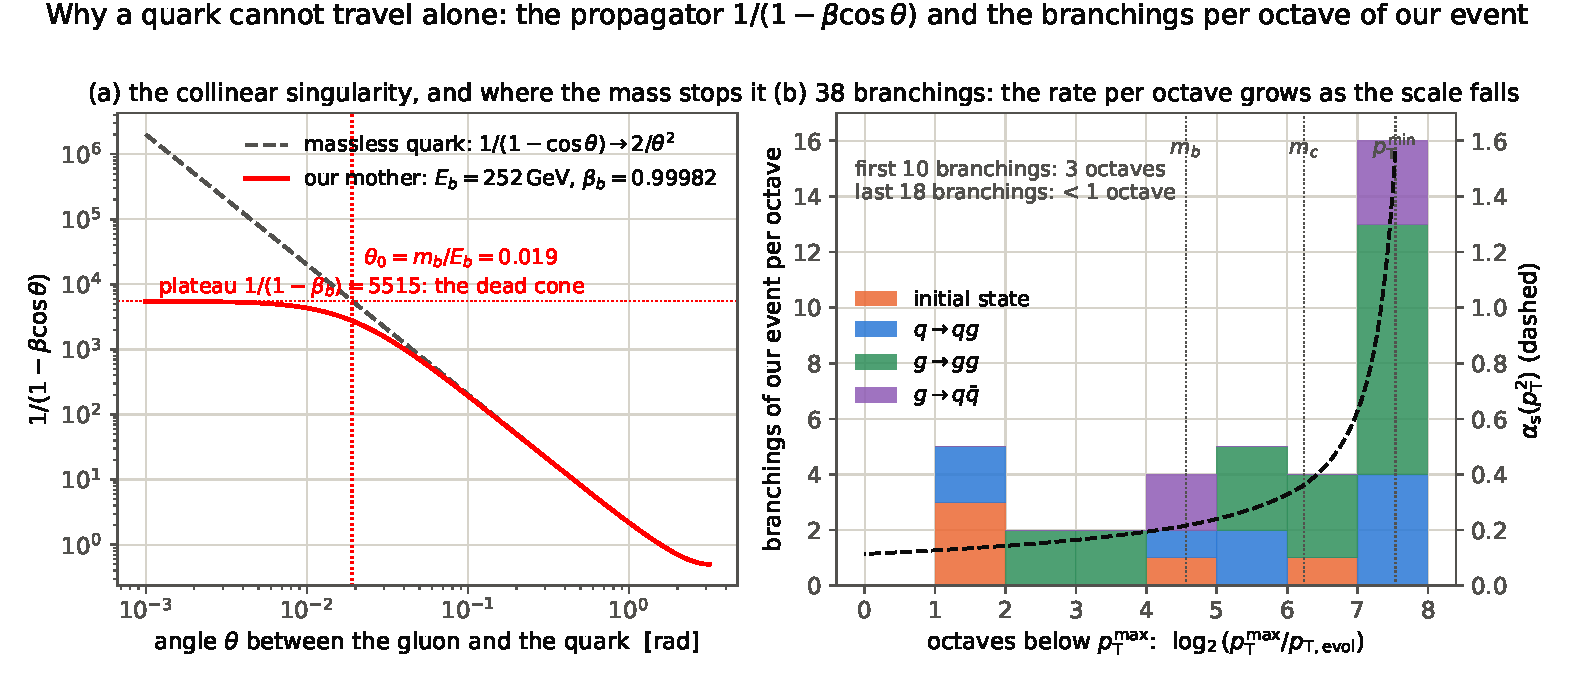
\includegraphics[page=1,width=\textwidth]{PS/Standalone/theory_parton_showering.pdf}
\caption[The collinear singularity and the branchings per octave of our event]{Why a quark cannot travel alone, from \file{plot_theory_PS.py}. (a) The factor $1/(1-\beta\cos\theta)$ of \cref{eq:mother_gives_birth:propagator} against the emission angle, for a massless quark and for our mother with $E_b=252\GeV$; the mass turns the singularity into a plateau below $\theta_0=\mb/E_b$. (b) The $38$ branchings of the seed-1 shower per octave of $\ptevol$ below $\pt^{\max}$, coloured by kind, with the running coupling on the right axis: the rate per octave grows as the scale falls, the $\mathrm{d}\theta^2/\theta^2$ measure of \cref{eq:mother_gives_birth:collinear_limit} helped by the growing coupling.}
\label{fig:mother_gives_birth:propagator_plot}
\end{figure}

Two remarks before we move on. First, the singularities are not artefacts:
they tell us that a bare quark is not an observable, and that any
calculation that stops at a fixed order needs to be combined with a
definition of what is measured, a jet, that is insensitive to arbitrarily
soft and collinear splittings. That is a theme for \cref{ch:the_inn}.
Second, the same structure appears for the \emph{incoming} partons. The
$\bar u$ and the $u$ that entered the hard process were resolved out of the
protons at the scale $\muF$, and the DGLAP evolution that produced the PDFs
of \cref{sec:ancestral_home:pdfs} is the very same
\cref{eq:mother_gives_birth:collinear_limit}, integrated over the angle. The
shower run backwards from the hard process undoes that evolution one step
at a time, and a parton emitted along the way is a real gluon or quark in
the final state. That is initial-state radiation, and we will see that in
our event it is louder than the mother's own.

\subsection{The splitting functions and the Sudakov form factor}
\label{sec:mother_gives_birth:splitting_sudakov}

\subsubsection{The four splitting functions}
\label{sec:mother_gives_birth:splitting_functions}

Set the stage before the formulas. After the three initial-state branchings
of our event there are five final-state partons and seven dipole ends;
after all thirty-eight there are forty partons and sixty-seven ends, and at every
round each of them may branch in one of several ways. A quark can only emit
a gluon. A gluon may emit a gluon or split into a quark--antiquark pair of
any flavour light enough at that scale. An incoming parton may be found to
come from a quark or from a gluon. So which kind of branching do you expect
to win most rounds, and which one almost never? Make your guess from three
things: the colour charge of the emitter, the number of emitters of each
kind at that moment, and whether the kernel favours a soft daughter. Then
compare with the list of our event: $38$ branchings, of which $5$ are
initial-state, $9$ are $q\to qg$, $19$ are $g\to gg$ and only $5$ are
$g\to q\bar q$. \Cref{fig:mother_gives_birth:ladder} shows
them in the order in which they happened; the functions that set these
proportions are the following.

\begin{figure}[htbp]\centering
\resizebox{\textwidth}{!}{% ---------------------------------------------------------------------------
% The four splitting functions as vertices, with their kernels, colour
% factors and the number of times each occurred among the 38 branchings of
% our event (-v log of standalone_parton_showering.py: 9 q->qg, 19 g->gg,
% 5 g->qqbar, 5 ISR of which 2 q<-q, 1 q<-g, 2 g<-g).
% ---------------------------------------------------------------------------
\begin{tikzpicture}[x=1cm,y=1cm,
  every node/.style={font=\footnotesize},
  fermion/.style={thick,postaction={decorate},decoration={markings,mark=at position 0.6 with {\arrow[scale=1.0]{Stealth}}}},
  antifermion/.style={thick,postaction={decorate},decoration={markings,mark=at position 0.4 with {\arrowreversed[scale=1.0]{Stealth}}}},
  gluon/.style={thick,decorate,decoration={coil,aspect=0,segment length=4pt,amplitude=1.8pt}},
  vertex/.style={fill=black,circle,inner sep=1.5pt},
  lab/.style={font=\scriptsize,align=center},
  kern/.style={font=\scriptsize,align=left},
  head/.style={font=\small\bfseries},
  count/.style={draw,rounded corners=2pt,fill=orange!20,font=\scriptsize,inner sep=2pt}]
\node[head,anchor=west] at (-0.4,2.6) {the four branchings of the shower, their kernels, and how often each happened in the 38 branchings of our event};
% (1) q -> q g
\begin{scope}
\draw[fermion] (0,0) -- (1.4,0); \draw[fermion] (1.4,0) -- (2.6,0.8) node[right,lab] {$q$, keeps $z$};
\draw[gluon] (1.4,0) -- (2.6,-0.8) node[right,lab] {$g$, takes $1-z$};
\node[vertex] at (1.4,0) {};
\node[lab,above] at (0.6,0.05) {$q$};
\node[kern,anchor=north west] at (-0.2,-1.3) {$P_{qq}(z)=C_F\dfrac{1+z^2}{1-z}$\\[3pt] soft pole at $z\to1$;\\$C_F=\tfrac43$};
\node[count] at (1.3,1.6) {$9\times$ ($b$, $\bar b$ and light quarks)};
\end{scope}
% (2) g -> g g
\begin{scope}[xshift=5.6cm]
\draw[gluon] (0,0) -- (1.4,0); \draw[gluon] (1.4,0) -- (2.6,0.8) node[right,lab] {$g$, $z$};
\draw[gluon] (1.4,0) -- (2.6,-0.8) node[right,lab] {$g$, $1-z$};
\node[vertex] at (1.4,0) {};
\node[lab,above] at (0.6,0.1) {$g$};
\node[kern,anchor=north west] at (-0.2,-1.3) {$P_{gg}(z)=2C_A\dfrac{(1-z(1-z))^2}{z(1-z)}$\\[3pt] poles at both ends;\\$C_A=3$, $C_A/C_F=\tfrac94$};
\node[count] at (1.3,1.6) {$19\times$, the most frequent};
\end{scope}
% (3) g -> q qbar
\begin{scope}[xshift=11.2cm]
\draw[gluon] (0,0) -- (1.4,0); \draw[fermion] (1.4,0) -- (2.6,0.8) node[right,lab] {$q$, $z$};
\draw[antifermion] (1.4,0) -- (2.6,-0.8) node[right,lab] {$\bar q$, $1-z$};
\node[vertex] at (1.4,0) {};
\node[lab,above] at (0.6,0.1) {$g$};
\node[kern,anchor=north west] at (-0.2,-1.3) {$P_{qg}(z)=T_R\,[z^2+(1-z)^2]$\\[3pt] no pole: a soft quark\\is not enhanced; $T_R=\tfrac12$};
\node[count] at (1.3,1.6) {$5\times$ ($s\bar s$, $\bbbar$, \dots)};
\end{scope}
% (4) initial state: q <- q, q <- g, g <- g, g <- q
\begin{scope}[xshift=16.8cm]
\draw[fermion] (0,0.8) -- (1.4,0) node[pos=0.1,above,lab] {$b$ from the proton, $x/z$};
\draw[fermion] (1.4,0) -- (2.8,0) node[right,lab] {$a$ into $\hat\sigma$, $x$};
\draw[gluon] (1.4,0) -- (2.4,-1.0) node[right,lab] {$c$ emitted};
\node[vertex] at (1.4,0) {};
\node[kern,anchor=north west] at (-0.2,-1.3) {backward: $P_{ba}(z)\,\dfrac{x'f_b(x',\pt^2)}{xf_a(x,\pt^2)}$\\[3pt] the same kernels read\\upstream, times a PDF ratio};
\node[count] at (1.3,1.6) {$5\times$ ($2\;q\leftarrow q$, $1\;q\leftarrow g$, $2\;g\leftarrow g$)};
\end{scope}
\node[lab,text=black!65,text width=19cm,anchor=north west] at (-0.4,-3.1) {The daughter that continues keeps the fraction $z$ of the parent's momentum; the kernels are rates per unit $\ln t$ and may exceed one. $P_{gq}(z)=P_{qq}(1-z)$ is the first vertex read with the gluon as the continuing parton, needed for $g\leftarrow q$ in the initial state. The gluon's double pole and its colour factor are why gluons take over the radiating as the shower proceeds: $27$ of the $40$ final partons of our event are gluons.};
\end{tikzpicture}
}
\caption[The four branchings of the shower as vertices, with their kernels and their counts in our event]{The four branchings of the shower as vertices: the parent on the left, the daughter that keeps the fraction $z$ above, the emitted parton below, with the kernel of \cref{eq:mother_gives_birth:splitting}, its colour factor and the number of times it occurred among the $38$ branchings of the seed-1 shower (\code{-v} log). The fourth vertex is the initial state: the same kernels read upstream, weighted by the ratio of parton densities of \cref{eq:mother_gives_birth:isr}.}
\label{fig:mother_gives_birth:splittings_sketch}
\end{figure}

Every branching of the shower is one of four, and the probability of each is
a leading-order Altarelli--Parisi splitting function of the momentum fraction
$z$~\cite{ParticleDataGroup:2024cfk}:
\begin{align}
  P_{qq}(z)&=C_F\,\frac{1+z^2}{1-z}, & &q\to qg, \notag\\
  P_{gg}(z)&=2C_A\left[\frac{z}{1-z}+\frac{1-z}{z}+z(1-z)\right]
            =2C_A\,\frac{\bigl(1-z(1-z)\bigr)^2}{z(1-z)}, & &g\to gg, \notag\\
  P_{qg}(z)&=T_R\left[z^2+(1-z)^2\right], & &g\to q\bar q, \label{eq:mother_gives_birth:splitting}\\
  P_{gq}(z)&=C_F\,\frac{1+(1-z)^2}{z}, & &q\to gq\ (\text{the gluon keeps }z), \notag
\end{align}
with $C_F=\tfrac43$, $C_A=3$ and $T_R=\tfrac12$. The first three are the
final-state branchings; the last is the first one read the other way round
and is needed for the initial state, where the parton that continues into the
hard process may be the gluon. Let me point at each as we pass. $P_{qq}$ and
$P_{gg}$ diverge as $1-z\to0$: that is the soft-gluon singularity of
\cref{eq:mother_gives_birth:propagator}, and $P_{gg}$ diverges at both ends
because either of the two gluons may be the soft one. $P_{qg}$ is finite:
a soft quark is not enhanced, which is why gluons split into quarks so much
less often than into gluons, and why in \cref{tab:mother_gives_birth:numbers}
three quarters of the final-state partons are gluons. The colour factors say
that a gluon radiates $C_A/C_F=9/4$ times more than a quark; a gluon jet is
broader and busier than a quark jet for exactly this reason, and every jet
tagger in the later chapters exploits it.

\Cref{tab:mother_gives_birth:kernels} evaluates the four kernels at the
$z$ values the shower of our event actually drew, so that the formulas
have faces. Two readings. Along a row, the gluon's $P_{gg}$ is always the
largest, by the factor $C_A/C_F$ and by its second pole. Down the
$q\to qg$ column, the kernel grows from $4.5$ for the mother's first
emission at $z=0.60$ to $145$ for the soft proposal at $z=0.98$ she made in
the first round; the latter was accepted and then lost, which is the
shower's way of saying that soft gluons are frequent but not important.

\begin{table}[htbp]\centering\small
\caption[The splitting functions at the $z$ of our event]{The four
splitting functions of \cref{eq:mother_gives_birth:splitting} at $z$
values drawn in the shower of our event; the bold entry is the kernel the
branching actually used. The kernels are rates, not probabilities, and
exceed one freely.}
\label{tab:mother_gives_birth:kernels}
\begin{tabular}{llrrrr}\toprule
branching & $z$ & $P_{qq}$ & $P_{gg}$ & $P_{qg}$ & $P_{gq}$ \\ \midrule
mother's first emission, $b\to bg$ (branching 5) & $0.601$ & $\mathbf{4.55}$ & $14.5$ & $0.26$ & $2.57$ \\
mother's first proposal, $b\to bg$ (round 1, lost) & $0.982$ & $\mathbf{145}$ & $326$ & $0.48$ & $1.36$ \\
$g\to gg$ (branching 6) & $0.275$ & $1.98$ & $\mathbf{19.3}$ & $0.30$ & $7.39$ \\
$g\to \bbbar$ (branching 10) & $0.350$ & $2.30$ & $15.7$ & $\mathbf{0.27}$ & $5.42$ \\
ISR $\bar u\leftarrow g$ (branching 1) & $0.779$ & $9.69$ & $23.9$ & $\mathbf{0.33}$ & $1.80$ \\
ISR $u\leftarrow u$ (branching 2) & $0.850$ & $\mathbf{15.3}$ & $35.7$ & $0.37$ & $1.61$ \\
ISR $g\leftarrow g$ (branching 3) & $0.206$ & $1.75$ & $\mathbf{25.7}$ & $0.34$ & $10.6$ \\
\bottomrule
\end{tabular}
\end{table}

One identity is worth checking yourself, because the standalone script relies
on it: the second form of $P_{gg}$ follows from the first by putting the three
terms over the common denominator $z(1-z)$ and recognising
$z^2+(1-z)^2+z^2(1-z)^2=(1-z+z^2)^2$. Exercise~2 asks for it.
\Cref{fig:mother_gives_birth:kernels_plot} draws the four kernels over the
whole range of $z$ with the $33$ final-state branchings of our event placed
on them, and the distribution of the $z$ values by kind: the quark
emissions cluster at $z>0.6$ where $P_{qq}$ is large, the gluon splittings
pile up at both ends where $P_{gg}$ has its two poles, and the five
$g\to q\bar q$ splittings sit where they fall, because $P_{qg}$ has no
preference.

\begin{figure}[htbp]\centering
\includegraphics[page=2,width=\textwidth]{PS/Standalone/theory_parton_showering.pdf}
\caption[The splitting functions and the $z$ values drawn in our event]{The splitting functions at work, from \file{plot_theory_PS.py}. (a) The four kernels of \cref{eq:mother_gives_birth:splitting} and the overestimate $2C_F/(1-z)$ of the veto algorithm; each dot is one of the $33$ final-state branchings of the seed-1 shower at its drawn $z$, the mother's two hardest emissions labelled. (b) The distribution of $z$ for the $38$ branchings by kind: soft daughters dominate the gluon splittings, the quark emissions of our event drew $z$ between $0.6$ and $1$.}
\label{fig:mother_gives_birth:kernels_plot}
\end{figure}

\begin{figure}[htbp]\centering
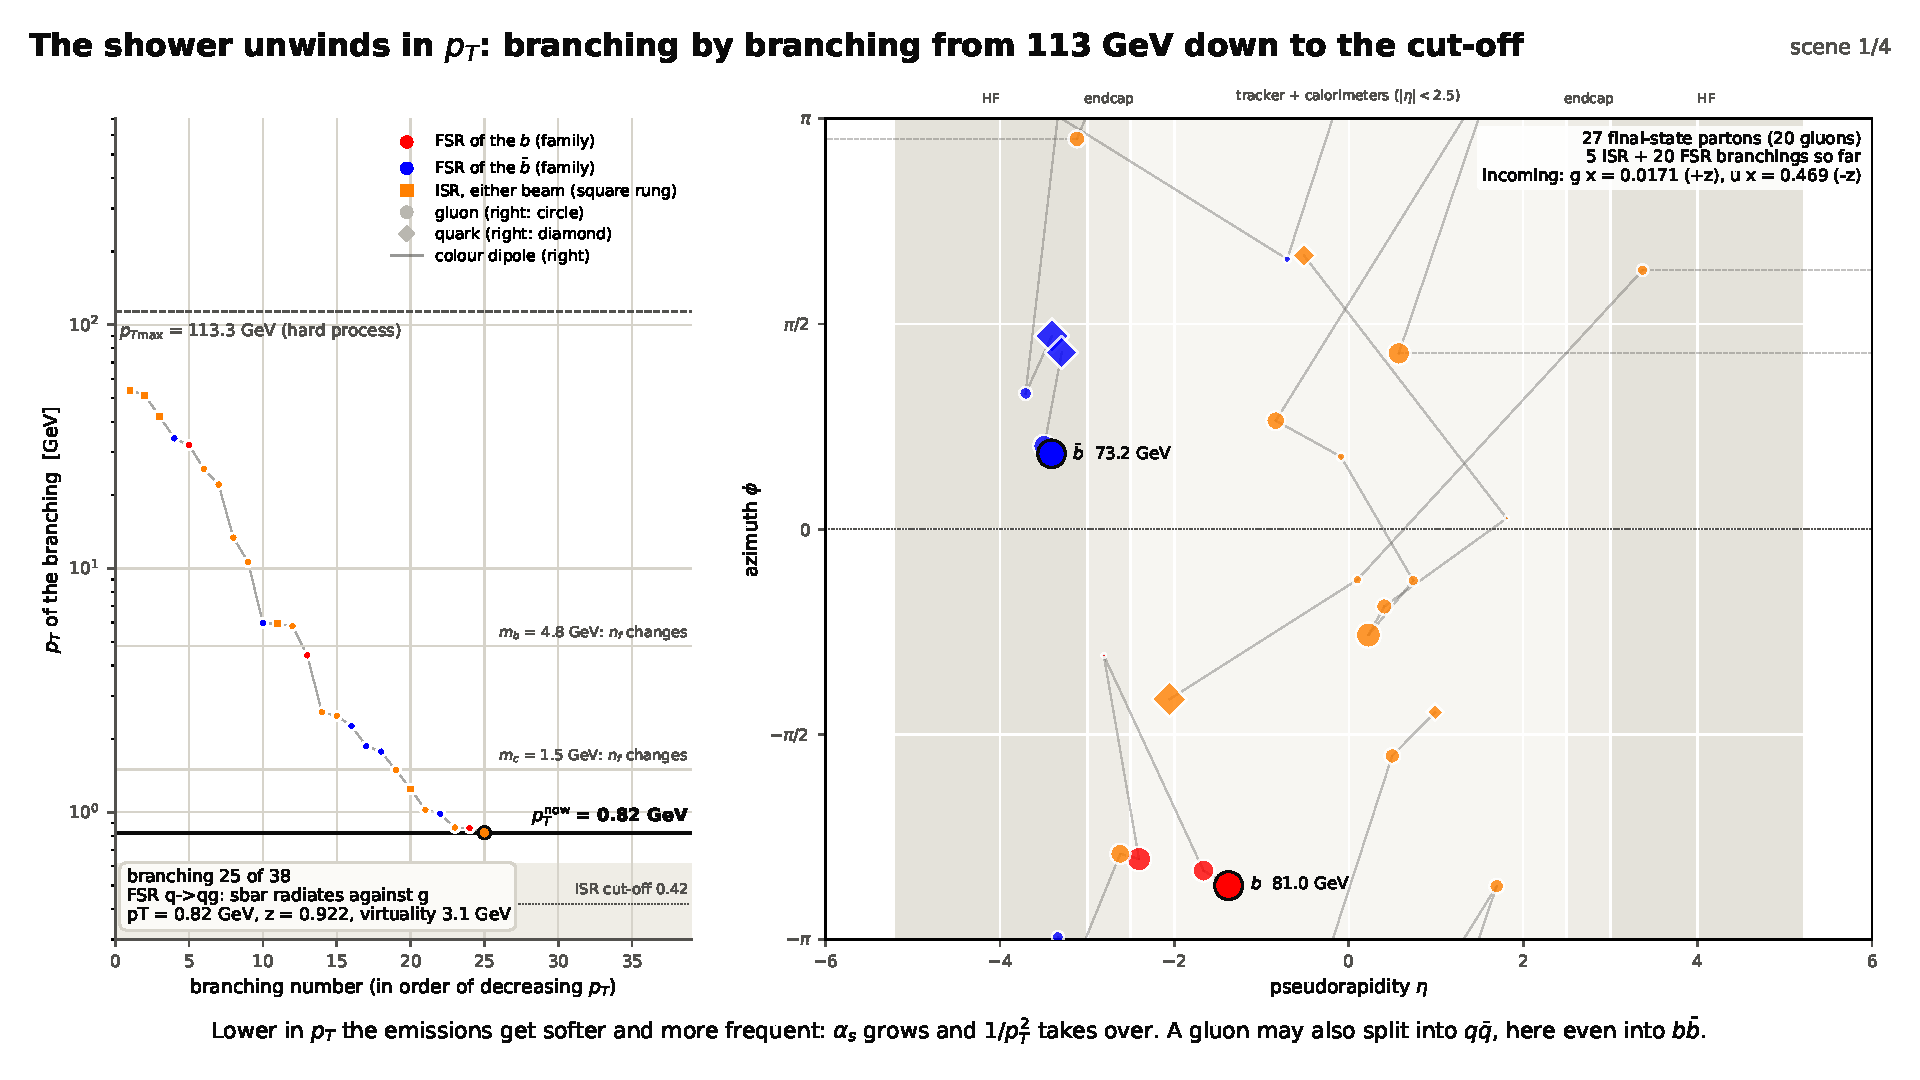
\includegraphics[page=1,width=\textwidth]{PS/Standalone/animate_standalone_parton_showering_stills.pdf}
\caption[The ladder of branchings of our event]{The first scene of the
film (\cref{sec:mother_gives_birth:animation}), stopped at branching 25 of
38. Left: the branchings of our event in decreasing \ptevol, orange squares
for the initial state, red and blue dots for the families of the $b$ and of
the $\bar b$. The rows of \cref{tab:mother_gives_birth:kernels} are rungs of
this ladder: the three orange squares at the top are the initial-state
branchings 1--3, the blue and red dots at rungs 4 and 5 are the first
emissions of the $\bar b$ and of the mother, rung 6 is the $g\to gg$ at
$25.6\GeV$ and rung 10 the $g\to\bbbar$ at $6.0\GeV$. Right: the
$(\eta,\phi)$ plane at that moment, with 27 final-state partons, 20 of them
gluons (circles) and 7 quarks (diamonds), joined by the colour dipoles that
do the radiating.}
\label{fig:mother_gives_birth:ladder}
\end{figure}

Now read the table and the figure together. The ladder is steep at the top
and flat at the bottom: the first ten branchings run from $53.9$ down to
$6.0\GeV$, three octaves, while the last eighteen all lie between
$1.02\GeV$ and the cut-off, less than one octave. That is the
$\mathrm{d}\theta^2/\theta^2$ measure of
\cref{eq:mother_gives_birth:collinear_limit} at work, helped by a coupling
that grows from $0.14$ at $30\GeV$ to $0.53$ at $1\GeV$: the number of
branchings per octave rises as the scale falls. Who branches is decided by
the kernels. Every branching adds a gluon to the final state, and a gluon
radiates with $C_A/2$ from each of its two colour lines, $C_A$ in all
against the quark's $C_F$, so
down the ladder the gluons take over the radiating: at rung 25 twenty of
the 27 partons are gluons, at the end 27 of 40, and 19 of the 38
branchings are $g\to gg$. The finite $P_{qg}$ keeps the $g\to q\bar q$
splittings to five, and because that kernel has no soft enhancement its
$z$ values, $0.35$ for the $g\to\bbbar$ of rung 10, sit in the middle of
the range rather than near the ends. The two quark emissions at rungs 4
and 5 both drew $z\approx0.6$, where $P_{qq}$ is a modest $4.5$; the soft
end of the kernel, where it reaches $145$ at $z=0.98$, produced the
mother's round-1 proposal at $5.2\GeV$, which lost. Soft emissions are the
most frequent, but in a shower ordered in \pt they come late.

\subsubsection{The Sudakov form factor}
\label{sec:mother_gives_birth:sudakov}

Start at the moment before the shower begins. Nothing has been emitted, so
for each of the four candidates, the $b$, the $\bar b$ and the two incoming
partons, the probability of having radiated is zero and the probability of
not having radiated is exactly one. Now let the scale run down from
$113\GeV$ and ask how that no-emission probability falls for each of them.
Guess before you look at \cref{fig:mother_gives_birth:survival}: which
curve falls fastest, and which two should lie on top of each other? The
$b$ and the $\bar b$ carry the same colour charge and sit in dipoles of the
same mass, $377.9\GeV$, so their curves must coincide. The two beams
differ: the $u$ at $x=0.39$ is a valence quark whose density falls when it
is asked for a larger $x$, while the $\bar u$ at $x=2.2\times10^{-3}$ can
be resolved out of a gluon density more than fifteen times larger. The end
whose curve falls fastest radiates first most often, and the figure,
measured by letting each end propose $1500$ times from $\pt^{\max}$,
confirms the guess: the $+z$ beam falls fastest and wins $53\%$ of the
first branchings, the $b$ and $\bar b$ curves lie on top of each other and
still stand at $0.8$ when the scale has fallen to $10\GeV$, and the dashed
product of all four is the probability that nobody has radiated yet. The
quantity on the vertical axis is the Sudakov form factor, and here is its
definition.

\begin{figure}[htbp]\centering
\includegraphics[page=2,width=\textwidth]{PS/Standalone/animate_standalone_parton_showering_stills.pdf}
\caption[Measured no-emission probabilities of the four radiators]{The
second scene of the film (\cref{sec:mother_gives_birth:animation}). Left:
the probability that an end has not yet radiated when the scale has fallen
from $\pt^{\max}=113.3\GeV$ to \pt, measured from $1500$ proposals per end
with the standalone shower; the dashed curve is the product of the four.
Right: who made the hardest of the four proposals, that is who radiates
first, as a histogram of that first scale. The first branching of the
seed-1 event, at $53.9\GeV$, is marked.}
\label{fig:mother_gives_birth:survival}
\end{figure}

Now the central object of the chapter. Take a parton produced at some hard
scale and ask: what is the probability that it does \emph{not} branch while
its evolution variable $t$ falls from $t_{\max}$ down to some $t$? Call the
branching probability per unit $\ln t$ at scale $t$
\begin{equation}
  \frac{\mathrm{d}\mathcal P}{\mathrm{d}\ln t}
  =\frac{\alphas(t)}{2\pi}\int_{z_{\min}}^{z_{\max}}\!\mathrm{d}z\,P(z)
  \equiv\frac{\alphas(t)}{2\pi}\,\hat P(t) ,
  \label{eq:mother_gives_birth:dP}
\end{equation}
where the $z$ limits depend on $t$ through the kinematics and keep the
integral finite. Divide the interval into many small steps; the probability
of surviving each step is one minus the probability of branching in it;
multiply them, take the limit, and you have
\begin{equation}
  \Delta(t_{\max},t)=\exp\left[-\int_{t}^{t_{\max}}\frac{\mathrm{d}t'}{t'}\,
  \frac{\alphas(t')}{2\pi}\,\hat P(t')\right],
  \label{eq:mother_gives_birth:sudakov}
\end{equation}
the Sudakov form factor. It is the same mathematics as radioactive decay
with a time-dependent decay rate, and it carries the same lesson: the
probability of the \emph{first} branching happening at $t$ is the rate at
$t$ times the probability of having survived down to $t$,
\begin{equation}
  \frac{\mathrm{d}\mathcal P_{\mathrm{first}}}{\mathrm{d}\ln t}
  =\frac{\alphas(t)}{2\pi}\,\hat P(t)\;\Delta(t_{\max},t)
  =-\frac{\mathrm{d}\Delta(t_{\max},t)}{\mathrm{d}\ln t}.
  \label{eq:mother_gives_birth:first}
\end{equation}
Integrate the right-hand side from $t_{\max}$ down to the cut-off $t_{\min}$
and you get $1-\Delta(t_{\max},t_{\min})$: the branching probabilities of
all scales, plus the probability of never branching, add up to one. This is
\emph{unitarity}, and it is the property that makes the shower a
probabilistic process rather than a perturbative expansion. The singular
kernels of \cref{eq:mother_gives_birth:splitting} are not a problem any more:
a divergence in $\hat P$ makes the form factor vanish, which just says that a
parton certainly branches before reaching the singular region.

\begin{figure}[htbp]\centering
\resizebox{\textwidth}{!}{% ---------------------------------------------------------------------------
% The Sudakov form factor as a product of survival probabilities, step by
% step down the scale, and its two faces (branch at t / never branch) with
% the numbers of our event (-v log: 3513 trials, 433 proposals, 33 winners
% for FSR; "no emission" in round 2 for the mother's end; 69 silent
% competitors in round 39).
% ---------------------------------------------------------------------------
\begin{tikzpicture}[x=1cm,y=1cm,
  every node/.style={font=\footnotesize},
  lab/.style={font=\scriptsize,align=center},
  head/.style={font=\small\bfseries},
  axis/.style={-{Stealth},thick},
  stepbox/.style={draw,thick,fill=blue!8,minimum height=7mm,minimum width=20mm,font=\scriptsize,align=center},
  branch/.style={draw,thick,fill=red!15,minimum height=7mm,minimum width=16mm,font=\scriptsize,align=center},
  flow/.style={-{Stealth},thick}]
% ---------------- (a) the product of survivals --------------------------------------------------
\node[head,anchor=west] at (-0.3,2.4) {(a) a no-emission probability is a product of survivals};
\draw[axis] (-0.3,0) -- (11.2,0); \node[lab,below] at (10.3,-0.1) {$\ln t$ runs \emph{down} $\to$};
\foreach \i/\x/\t in {1/0.3/{$t_{\max}$},2/2.6/{$t_1$},3/4.9/{$t_2$},4/7.2/{$t_3$},5/9.5/{$\cdots$}} {
  \draw (\x,-0.1) -- (\x,0.1); \node[lab,below] at (\x,-0.1) {\t};}
\foreach \x/\lab in {1.45/{$1-\frac{\alphas\hat P}{2\pi}\delta\ln t\big|_{t_1}$},3.75/{$1-\frac{\alphas\hat P}{2\pi}\delta\ln t\big|_{t_2}$},6.05/{$1-\frac{\alphas\hat P}{2\pi}\delta\ln t\big|_{t_3}$},8.35/{$\cdots$}} {
  \node[stepbox] at (\x,0.9) {\lab};}
\node[lab] at (9.9,0.9) {$\times\;\cdots$};
\node[lab,text=black!65,text width=10.4cm,anchor=north west] at (-0.3,-0.75) {Survive the first step, \emph{and} the second, \emph{and} the third: multiply. In the limit $\delta\ln t\to0$ the product becomes $\exp[-\int\mathrm{d}\ln t\,\frac{\alphas}{2\pi}\hat P]=\Delta(t_{\max},t)$, \cref{eq:mother_gives_birth:sudakov}, the same mathematics as a decay with a time-dependent rate. The probability of the \emph{first} branching at $t$ is the rate there times the survival down to there, \cref{eq:mother_gives_birth:first}.};
% ---------------- (b) two faces -------------------------------------------------------------
\begin{scope}[xshift=13.4cm]
\node[head,anchor=west] at (-0.3,2.4) {(b) the two faces in the log of our event};
\node[stepbox,minimum width=30mm] (S) at (1.6,1.2) {a dipole end at scale $t_{\max}$};
\node[branch,minimum width=30mm] (B) at (-0.6,-0.6) {``proposes \dots\ pT = \dots''\\branches at $t$};
\node[stepbox,minimum width=30mm,fill=gray!12] (N) at (3.8,-0.6) {``no emission above\\the cut-off''};
\draw[flow] (S) -- (B) node[midway,left,lab] {$1-\Delta(t_{\max},t_{\min})$};
\draw[flow] (S) -- (N) node[midway,right,lab] {$\Delta(t_{\max},t_{\min})$};
\node[lab,text=black!65,text width=7.4cm,anchor=north west] at (-2.1,-1.35) {The two add up to one: unitarity. In round~2 the mother's own end took the right branch from $53.9\GeV$ straight through the cut-off; in round~39 all $69$ competitors did, and the shower stopped. Three levels of bookkeeping over the event: $3513$ trial scales, $433$ accepted proposals, $33$ winners (final state).};
\end{scope}
\end{tikzpicture}
}
\caption[The Sudakov form factor as a product of survival probabilities, and its two faces in the log]{(a) The no-emission probability as a product of survivals: divide the evolution in $\ln t$ into small steps, survive each with probability one minus the branching probability of the step, and multiply; the limit is the exponential of \cref{eq:mother_gives_birth:sudakov}. (b) The two faces of the form factor in the \code{-v} log of our event: every line that reads ``proposes'' is the branching face, every ``no emission above the cut-off'' is the surviving face, and the two add up to one. The counts are those of the seed-1 shower.}
\label{fig:mother_gives_birth:sudakov_sketch}
\end{figure}

The log shows both faces of the form factor. The ``branches at $t$'' face
is every line that reads ``proposes''; the ``never branches'' face is every
line that reads ``no emission above the cut-off'', and the second kind
appears already in round~2 of our event, where the mother's own dipole end
evolved from $53.9\GeV$ straight through the cut-off without an accepted
emission, and dominates the end: in round~39 all $69$ competitors ($67$
colour ends of the $40$ final partons plus the two beams) propose nothing,
and the shower stops. Over the whole event the veto algorithm generated
$3513$ final-state and $212$ initial-state trials, of which $433$ and $34$
survived their own acceptance tests and $33$ and $5$ won their round. Three
levels, then: a trial is a random number, an accepted proposal is a
possible emission, and only the winner of a round becomes a parton.

\paragraph{The double logarithm, once by hand.} Let me do for the mother
what we did with the Jacobian at the previous stop, because every shower
hides it. Keep only the soft-collinear part of $P_{qq}$, $2C_F/(1-z)$,
use as evolution variable the transverse momentum $\pt$ of the emission with
respect to the emitter, and take as $z$ limit the collinear kinematics
$1-z\ge\pt/Q$ for a parton of energy of order $Q$. Then
$\hat P=2C_F\ln(Q/\pt)$ and, for a fixed coupling,
\begin{equation}
\begin{split}
  -\ln\Delta(\pt^{\max},\pt)
  &=\frac{\alphas C_F}{\pi}\int_{\pt}^{\pt^{\max}}\frac{2\,\mathrm{d}q}{q}\ln\frac{Q}{q}
  =\frac{\alphas C_F}{\pi}\left[\ln^2\frac{Q}{\pt}-\ln^2\frac{Q}{\pt^{\max}}\right].
\end{split}
  \label{eq:mother_gives_birth:double_log_sudakov}
\end{equation}
Differentiate $\ln^2(Q/q)$ with respect to $q$ to check the integral; you
get $-2\ln(Q/q)/q$. For our mother the natural $Q$ is the mass of the
colour dipole she forms with the incoming $u$ quark,
$Q^2=(p_b+p_u)^2=2\mb^2-\hat t=1.43\times10^{5}\GeV^2$, that is
$Q=378\GeV$ (the invariants are in the Info Listing of the \CMSSW log,
\cref{sec:ancestral_home:cmssw}), and the shower starts at
$\pt^{\max}=113.3\GeV$ (\cref{sec:mother_gives_birth:scales}). With
$\alphas=0.118$ the probability that she emits nothing above $10\GeV$ is
\begin{equation*}
  \Delta(113.3,10)=\exp\left\{-0.0501\left[\ln^2 37.8-\ln^2 3.34\right]\right\}
  =\exp(-0.588)=0.56 ,
\end{equation*}
and with the running coupling of \cref{sec:mother_gives_birth:cp5} in the
integrand it drops to $0.48$. Scene~2 of the film (\cref{sec:mother_gives_birth:animation})
measured the same quantity from the standalone shower itself and found
about $0.8$ (\cref{fig:mother_gives_birth:sudakov_plot}). The difference is what the leading logarithm leaves out: the
full kernel is smaller than $2C_F/(1-z)$ away from $z=1$, the exact $z$
range of the dipole is narrower than $1-z\ge\pt/Q$, and an emission that
recoils against an incoming parton is further weighted by the PDF ratio
and by a damping factor described in \cref{sec:mother_gives_birth:fsr}.
The estimate is nevertheless worth having: it tells you at a glance that a
$100\GeV$ quark radiates a $10\GeV$ gluon about half the time, a
$1\GeV$ gluon almost always, and it shows why the evolution must be cut off
at some $\pt^{\min}$ where the coupling stops making sense.
\Cref{fig:mother_gives_birth:sudakov_plot} puts the estimate next to the
measured curves: the leading-logarithmic form factor with a fixed and with a
running coupling, both for the mother's dipole, against the survival
probabilities of all four radiators measured from $1500$ proposals each
with the shower script itself, the same measurement as scene~2 of the film.
The two leading-log curves fall below the measured one for the reasons
listed above, and all three agree that the mother emits nothing above
$30\GeV$ in most showers and nothing above $1\GeV$ almost never.

\begin{figure}[htbp]\centering
\includegraphics[page=3,width=\textwidth]{PS/Standalone/theory_parton_showering.pdf}
\caption[The measured Sudakov form factors against the leading-log formula]{The Sudakov form factor, from \file{plot_theory_PS.py}. (a) The probability that each of the four radiators of the hard event has not yet branched when the scale has fallen from $\pt^{\max}$ to \pt, measured from $1500$ proposals per radiator with the veto algorithm of the script; the dashed black curve is their product. For the mother's dipole the leading-logarithmic estimate \cref{eq:mother_gives_birth:double_log_sudakov} is drawn with a fixed coupling (dotted) and with the running coupling in the integrand (dash-dotted). (b) The scale of the first branching, the hardest of the four proposals, coloured by who made it; the $+z$ beam at small $x$ wins most often, as in the seed-1 event.}
\label{fig:mother_gives_birth:sudakov_plot}
\end{figure}

\subsubsection{From a form factor to a random number: the veto algorithm}
\label{sec:mother_gives_birth:veto}

The form factor gives a probability; the computer needs a scale. Picture
the mother at $113.3\GeV$ in round~1 with her survival curve of
\cref{fig:mother_gives_birth:survival} in front of her. To decide where she
branches next she should draw a uniform random number $R$, go to the height
$R$ on that curve and read off the \pt, exactly as one samples a decay time
from an exponential. The curve, however, is an integral over the full
kernel and the running coupling and has no closed form, so nothing can be
read off it. The way out is the oldest trick of Monte Carlo: replace the
curve by a simpler one that lies \emph{below} it everywhere, that is, one
that overestimates the branching rate; sample from that; then throw away
the surplus with a second random number. \Cref{fig:mother_gives_birth:veto}
shows the four steps with the mother's own numbers; keep it open while you
read them.

\begin{figure}[htbp]\centering
\resizebox{\textwidth}{!}{% ---------------------------------------------------------------------------
% The Sudakov veto algorithm as a flow chart, annotated with the mother's
% first proposal in round 1 of the seed-1 shower (-vv log): three draws,
% 59.67 -> 47.54 -> 5.24 GeV, the four weight factors and R' = 0.062.
% ---------------------------------------------------------------------------
\begin{tikzpicture}[x=1cm,y=1cm,
  every node/.style={font=\footnotesize},
  box/.style={draw,rounded corners=3pt,thick,fill=orange!12,align=center,inner sep=5pt,text width=4.6cm},
  decision/.style={draw,thick,diamond,aspect=2.6,fill=blue!8,align=center,inner sep=1pt,text width=3.6cm,font=\scriptsize},
  numbox/.style={draw,rounded corners=3pt,thin,fill=blue!6,align=left,inner sep=4pt,text width=6.9cm,font=\scriptsize},
  flow/.style={-{Stealth[length=2.5mm,width=2mm]},thick},
  no/.style={flow,red!70!black},
  yes/.style={flow,green!50!black},
  head/.style={font=\small\bfseries},
  lab/.style={font=\scriptsize,align=center}]
\node[head,anchor=west] at (-2.6,1.4) {the veto algorithm, one proposal};
\node[head,anchor=west] at (7.0,1.4) {the mother's proposal in round 1 (\code{-vv} log)};
\node[box] (A) at (0,0) {\textbf{start} at the current scale $t$ (first: $t_{\max}$)};
\node[box,below=6mm of A] (B) {\textbf{draw $R$}, solve $\Delta_{\mathrm{over}}(t,t')=R$ for the next trial scale $t'$ (\cref{eq:mother_gives_birth:veto_solution})};
\node[decision,below=6mm of B] (C) {$t'$ above the cut-off and kinematically allowed?};
\node[box,below=6mm of C] (D) {\textbf{draw $z$} from the overestimate kernel; compute the weight $w$ of \cref{eq:mother_gives_birth:veto_weight}};
\node[decision,below=6mm of D] (E) {draw $R'$: $R'\le w$?};
\node[box,below=6mm of E,fill=green!12] (F) {\textbf{accept}: this end proposes $t'$, $z$ (it still has to win the round)};
\node[box,fill=gray!12] (G) at (-6.4,0 |- C) {\textbf{no emission}: this end is silent in this round};
\draw[flow] (A) -- (B); \draw[flow] (B) -- (C); \draw[yes] (C) -- (D) node[midway,right,lab] {yes}; \draw[flow] (D) -- (E); \draw[yes] (E) -- (F) node[midway,right,lab] {yes};
\draw[no] (C) -- (G) node[pos=0.3,above,lab] {below the cut-off};
\draw[no] (E.east) -- ++(1.6,0) |- (A.east); \node[lab,text=red!70!black,anchor=west] at (4.3,0 |- E) {no: \textbf{continue from $t'$},\\not from $t_{\max}$};
\draw[no] (C.east) -- ++(1.0,0) |- ($(A.east)+(0,-0.25)$); \node[lab,text=red!70!black,anchor=west] at (4.3,0 |- C) {not allowed:\\continue from $t'$};
% the numbers
\node[numbox,anchor=west] (N1) at (7.0,0 |- B) {draw 1: $R=0.51607$ from $113.32\GeV$ $\to$ $t'^{1/2}=59.67\GeV$};
\node[numbox,anchor=west] (N2) at (7.0,0 |- C) {$59.67$: recoiler is the incoming $u$, would need $x'=2.65>1$: not allowed\\draw 2: $R=0.77668$ from $59.67$ $\to$ $47.54\GeV$: $x'=19$, not allowed\\draw 3: $R=0.03959$ from $47.54$ $\to$ $5.24\GeV$: allowed};
\node[numbox,anchor=west] (N3) at (7.0,0 |- D) {$z=0.9819$ from $2C_F/(1-z)$;\quad $w=0.9818\times0.8076\times0.2747\times0.9810=0.2137$\\(kernel ratio, coupling ratio, beam-recoil damping, PDF ratio)};
\node[numbox,anchor=west] (N4) at (7.0,0 |- E) {$R'=0.0623\le0.2137$: accepted};
\node[numbox,anchor=west] (N5) at (7.0,0 |- F) {the mother proposes $5.241\GeV$, $z=0.9819$; the $+z$ beam proposes $53.877\GeV$ and wins the round. Over the event: $3513$ draws, $433$ accepted, $33$ winners.};
\foreach \s/\n in {B/N1,C/N2,D/N3,E/N4,F/N5} {\draw[flow,gray!60] ($(\s.east)+(0.1,0)$) -- (\n.west);}
\end{tikzpicture}
}
\caption[The veto algorithm as a flow chart, with the mother's first proposal]{The veto algorithm as a flow chart. Left: one proposal of one radiator, from the current scale to an accepted trial or to silence; the two red loops are the instruction that makes the algorithm exact, to continue from the rejected scale and not from $t_{\max}$. Right: the mother's proposal in round~1 of the seed-1 shower from the \code{-vv} log, three draws and four weight factors long, which produced the $5.24\GeV$ that lost to the $+z$ beam.}
\label{fig:mother_gives_birth:veto_flow}
\end{figure}

\begin{figure}[htbp]\centering
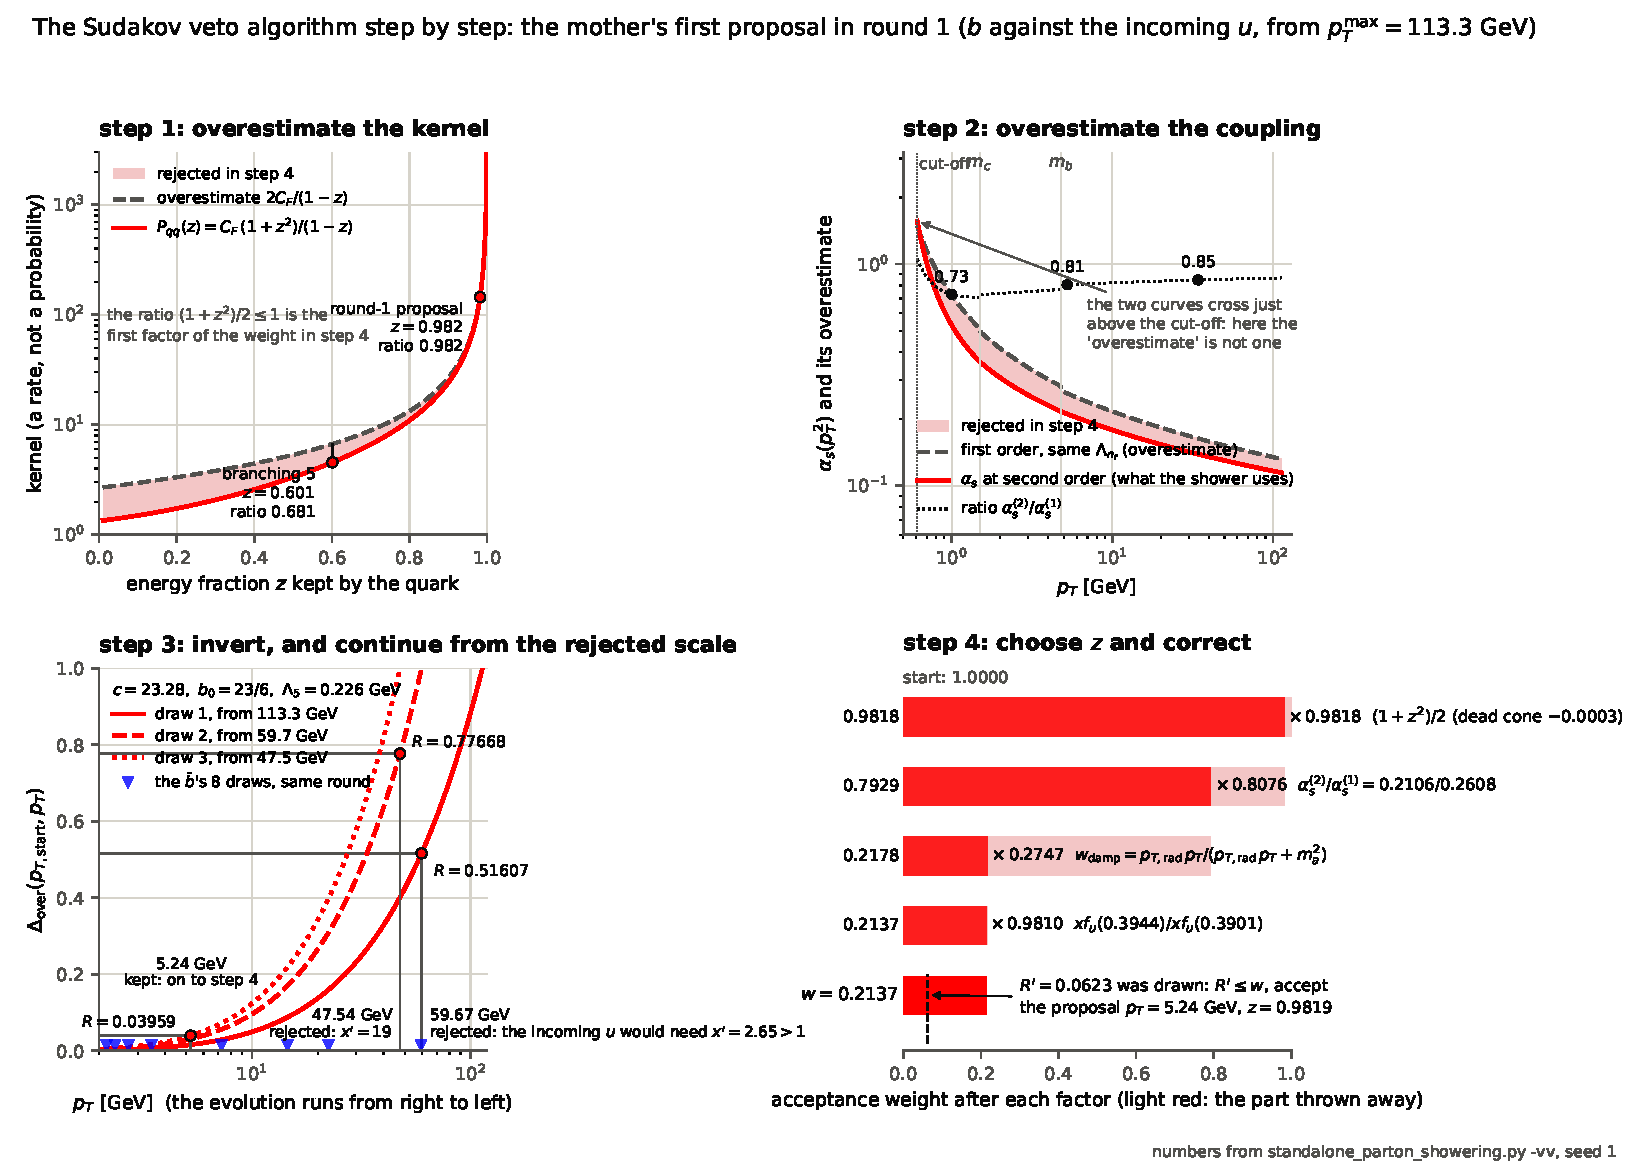
\includegraphics[width=\textwidth]{PS/Standalone/veto_algorithm.pdf}
\caption[The veto algorithm step by step]{The four steps of the veto
algorithm for the mother's first proposal in round~1, drawn by
\file{plot\_veto\_algorithm.py} from the \code{-vv} log. Step~1: the kernel
$P_{qq}$ and its overestimate $2C_F/(1-z)$; the shaded surplus is removed in
step~4, and the two $z$ values of the mother's emissions are marked.
Step~2: the second-order coupling and its first-order overestimate, with
the ratio that becomes a weight; in the last octave above the cut-off the
two curves cross. Step~3: the overestimated form factor
$\Delta_{\mathrm{over}}$ for three draws in a row, each starting from the
scale the previous one reached: $R=0.516$ gives $59.7\GeV$, rejected
because the incoming $u$ would need $x'>1$; $R=0.777$ from $59.7\GeV$ gives
$47.5\GeV$, rejected for the same reason; $R=0.040$ from $47.5\GeV$ gives
$5.24\GeV$. The blue triangles are the eight draws the $\bar b$ needed in
the same round. Step~4: the four factors of the acceptance weight of the
$5.24\GeV$ trial, the light part of each bar being thrown away, and the
$R'=0.062$ that accepted it.}
\label{fig:mother_gives_birth:veto}
\end{figure}

Here is the part I would like you to do once with pencil and paper, because
it is the engine of every shower and it fits on half a page. We want to
sample the scale of the next branching from \cref{eq:mother_gives_birth:first},
that is, to solve $\Delta(t_{\max},t)=R$ for $t$ with $R$ uniform in
$[0,1]$. For the real $\hat P(t)$ and the real $\alphas(t)$ that cannot be
done in closed form. So replace both by overestimates that can be inverted,
and correct afterwards.

\paragraph{Step 1: overestimate the kernel.} Choose a constant
$\hat P_{\mathrm{over}}\ge\hat P(t)$ for all $t$ in the interval. For
$P_{qq}$ the script uses $2C_F/(1-z)$ integrated over the widest $z$ range
that occurs in the interval, $c\equiv2C_F\ln\frac{1-z_{\min}}{1-z_{\max}}$;
the missing factor $(1+z^2)/2\le1$ is applied later. For the mother's
dipole in round~1 the $z$ range is set by the lowest scale of the
five-flavour segment, $\pt=\mb$, on a dipole of corrected mass squared
$(377.9\GeV)^2-\mb^2=1.428\times10^5\GeV^2$:
$z_{\min}=\tfrac12-\sqrt{\tfrac14-23.04/1.428\times10^5}=1.6\times10^{-4}$,
$z_{\max}=1-z_{\min}$, and $c=\tfrac83\ln(0.99984/0.00016)=23.28$. The
top-left panel of \cref{fig:mother_gives_birth:veto} shows the two
curves; the band between them is what step~4 will throw away.

\paragraph{Step 2: overestimate the coupling.} Use the first-order form
\begin{equation}
  \alphas^{(1)}(t)=\frac{2\pi}{b_0\ln(t/\Lambda^2)},\qquad
  b_0=\frac{33-2n_f}{6},
  \label{eq:mother_gives_birth:alphas_1loop}
\end{equation}
which for the same $\Lambda$ lies above the second-order running (the
correction term is negative) and which has an elementary integral. The
log prints both at the scales that matter: at $34.2\GeV$, where the
$\bar b$ first radiates, $0.1633$ against the true $0.1386$; at $5.2\GeV$,
$0.2608$ against $0.2106$; at $1\GeV$, $0.725$ against $0.530$. The ratio,
$0.85$, $0.81$ and $0.73$, is the price of the overestimate and returns as
a weight in step~4. In the last octave above the cut-off the two curves
cross: at $0.611\GeV$ the first-order form gives $1.485$ and the
second-order $1.563$, a ratio of $1.052$, and the ``overestimate'' is no
longer one. The top-right panel shows the two curves crossing there.

\paragraph{Step 3: invert.} With these two,
\begin{equation}
  -\ln\Delta_{\mathrm{over}}(t_{\max},t)
  =\int_t^{t_{\max}}\frac{\mathrm{d}t'}{t'}\,\frac{c}{b_0\ln(t'/\Lambda^2)}
  =\frac{c}{b_0}\ln\frac{\ln(t_{\max}/\Lambda^2)}{\ln(t/\Lambda^2)},
\end{equation}
because $\mathrm{d}t'/t'=\mathrm{d}\ln t'$ and
$\int\mathrm{d}u/u=\ln u$ with $u=\ln(t'/\Lambda^2)$. Setting this equal to
$-\ln R$ and solving for $t$,
\begin{equation}
  \ln\frac{t}{\Lambda^2}=\ln\frac{t_{\max}}{\Lambda^2}\;R^{\,b_0/c}
  \qquad\Longrightarrow\qquad
  t=\Lambda^2\left(\frac{t_{\max}}{\Lambda^2}\right)^{R^{\,b_0/c}} .
  \label{eq:mother_gives_birth:veto_solution}
\end{equation}
This single line is what the standalone script executes at every trial
(\code{pT2next\_fsr}, \code{pT2next\_isr}); find it on GitHub and you will
recognise $\Lambda^2$, $b_0$ and $c$. Check the limits: $R=1$ gives
$t=t_{\max}$ (no evolution), $R\to0$ gives $t\to\Lambda^2$ (the coupling
blows up), and a large $c$, that is a strongly radiating parton, pushes $t$
towards $t_{\max}$. Now do it with the mother's numbers of round~1,
$t_{\max}=113.32^2\GeV^2$, $\Lambda_5=0.2262\GeV$, $b_0=23/6=3.833$ and
$c=23.28$, so that $b_0/c=0.1646$. The \code{-vv} log drew
$R=0.51607$: $R^{0.1646}=0.8968$, $\ln(t_{\max}/\Lambda_5^2)=12.433$, and
\cref{eq:mother_gives_birth:veto_solution} gives
$\sqrt t=0.2262\,\mathrm{e}^{0.8968\times12.433/2}=59.67\GeV$. One random
number has taken the mother from $113.3$ to $59.7\GeV$; the next two, in
the same log, took her from $59.7$ to $47.5$ and from $47.5$ to
$5.24\GeV$. Why three draws for one proposal is the business of step~4.
The bottom-left panel draws the three curves $\Delta_{\mathrm{over}}$ of
these draws, each one starting where the previous one stopped; a single
curve from $113\GeV$ would have been the wrong distribution.

\paragraph{Step 4: choose $z$ and correct.} Draw $z$ from the overestimate
kernel (for $2C_F/(1-z)$ that is $1-z=(1-z_{\min})[(1-z_{\max})/(1-z_{\min})]^{R'}$),
then accept the trial with probability
\begin{equation}
  w=\frac{P(z)}{P_{\mathrm{over}}(z)}\times\frac{\alphas(t)}{\alphas^{(1)}(t)}
  \times(\text{any further factor}\le1),
  \label{eq:mother_gives_birth:veto_weight}
\end{equation}
and if it is rejected, \emph{continue the evolution from the rejected $t$},
not from $t_{\max}$. That last instruction is the veto algorithm proper, and
it is the step people get wrong. Restarting from $t_{\max}$ would sample
$\Delta_{\mathrm{over}}$ and then thin it; continuing from the rejected scale
samples exactly $\Delta$ with the true kernel, because the survival
probability of the true process factorises through every intermediate scale.
Exercise~4 asks you to prove it for a two-step interval. All further physics,
the second-order coupling, the mass term of the heavy quark, the PDF ratio
of an incoming recoiler, is inserted through the weight of
\cref{eq:mother_gives_birth:veto_weight}, which is why the script can count
how often a weight exceeded one (14 times in our event, all from the
coupling ratio in the last octave above the cut-off, where the second-order
running is no longer below the first-order form).

Here is the mother's first proposal, trial by trial, from the \code{-vv}
log. The first draw, $59.7\GeV$, was rejected before any weight was
computed: the recoiler is the incoming $u$, and absorbing that virtuality
would have needed $x'=2.65$, more than the whole proton. The second,
$47.5\GeV$, failed the same test with $x'=19$. The evolution continued
from $47.5\GeV$, not from $113\GeV$, and the third draw gave $5.24\GeV$
with $z=0.9819$ from the overestimate kernel. Then the weight of
\cref{eq:mother_gives_birth:veto_weight}, factor by factor:
\begin{equation*}
  w=\underbrace{0.9818}_{(1+z^2)/2\text{, dead cone }0.0003}
  \times\underbrace{0.8076}_{0.2106/0.2608}
  \times\underbrace{0.2747}_{w_{\mathrm{damp}}\text{, \cref{eq:mother_gives_birth:dampen}}}
  \times\underbrace{0.9810}_{xf_u(0.3944)/xf_u(0.3901)}
  =0.2137 ,
\end{equation*}
against which $R'=0.0623$ was drawn: accepted (the bottom-right panel of
\cref{fig:mother_gives_birth:veto}). That is the ``$5.241\GeV$,
$z=0.9819$'' the mother proposed in round~1, and it lost to the
$53.9\GeV$ of the $+z$ beam. The same three-level bookkeeping, trials,
accepted proposals, winners, gave the $3513/433/33$ of
\cref{sec:mother_gives_birth:sudakov}.

\subsection{\PYTHIA's \texorpdfstring{\pt}{pT}-ordered dipole shower}
\label{sec:mother_gives_birth:dipole_shower}

What is the evolution variable $t$? Angle, virtuality and transverse
momentum have all been used; \PYTHIA~8 uses the transverse momentum of the
branching~\cite{Sjostrand:2004ef,Bierlich:2022pfr}, and its radiators are
not single partons but colour dipoles. The standalone script of
\cref{sec:mother_gives_birth:standalone_code} follows that construction
closely enough that its output can be compared with the generator's, and
this section describes the construction with the script's variable names in
brackets, so that you can read the two side by side.

\subsubsection{Final-state radiation}
\label{sec:mother_gives_birth:fsr}

Whom does the mother radiate against? The natural guess is her twin, the
$\bar b$ she was born with, and it is wrong: the two quarks of our hard
process are not colour-connected to each other at all, and the mother's
partner is a parton in the beam. That one fact decides the recoil of every
one of her emissions, so it has to be settled before the kinematics.
Start from what the two colour columns of \file{event_ME.lhe} record. A
quark carries one of $N_c=3$ colours, an antiquark one of three
anticolours, and a gluon one colour and one anticolour, eight of the nine
combinations, since the colour-singlet one is not a gluon. A generator does
not propagate SU(3) amplitudes through forty branchings. It keeps the
leading term of the expansion in $1/N_c$, in which the colour structure of
any diagram is a set of \emph{lines}, each carrying one colour index
unchanged from where it starts to where it ends: a quark is one line
pointing along its motion, an antiquark one line pointing against it, and
a gluon is a pair of lines with opposite arrows, 't~Hooft's double-line
notation. The Les Houches record numbers the lines from 101 upwards, and
the two colour columns of a parton are the tags of the line and the
anti-line it holds. For our hard process the assignment follows from one
identity. The $s$-channel gluon couples the two quark currents through
\begin{equation}
  T^a_{ij}\,T^a_{kl}
  =\frac12\left(\delta_{il}\delta_{jk}-\frac{1}{N_c}\,\delta_{ij}\delta_{kl}\right),
  \label{eq:mother_gives_birth:fierz}
\end{equation}
where $j$ and $i$ are the colour indices of the incoming $u$ and $\bar u$
and $k$ and $l$ those of the outgoing $b$ and $\bar b$. The first term
identifies the colour of the $u$ with that of the $b$ and the anticolour
of the $\bar u$ with that of the $\bar b$; the second, a colour-singlet
exchange suppressed by $1/N_c$, is dropped. That is
\cref{fig:mother_gives_birth:dipoles}(a): colour~102 runs from the
incoming $u$ through the virtual gluon to the $b$, anticolour~101 from the
incoming $\bar u$ to the $\bar b$, and nothing connects the mother to her
twin. Her colour partner is a beam parton. The price of the approximation
is of order $1/N_c^2$, and \PYTHIA recovers part of it by letting a quark
end radiate with $C_F=4/3$ rather than with the strict large-$N_c$ value
$N_c/2$.

Every final-state parton with a colour line thus has a partner at the
other end of that line, and a gluon has two lines and therefore two
partners. Each such pair is a \emph{dipole}, and each end of a dipole is a
radiator, with the other end as its \emph{recoiler} [\code{dipole\_ends}].
The initial-state shower rethreads the lines too.
\Cref{fig:mother_gives_birth:dipoles}(b) shows branching~1
(\cref{sec:mother_gives_birth:isr}): backward evolution finds that the
$\bar u$ came out of a gluon, and a gluon holds two lines, the 101 that the
$\bar u$ already had, which now begins at the beam gluon \#7, and a new
103 that leaves with the emitted $u$ \#8. The hard process is untouched,
but the dipole 101 has a new end and its mass has grown from $377.9$ to
$420.5\GeV$ (step~2 of the log). The dipole picture is what makes the
shower coherent: a soft gluon at a wide angle sees the total colour charge
of the pair, not of one parton, and interference between the two ends is
built in (\cref{fig:mother_gives_birth:dipoles}(e)). The same lines
outlive the shower: hadronisation will stretch a string along every one of
them (\cref{ch:children_getting_married}).

\begin{figure}[htbp]\centering
\resizebox{\textwidth}{!}{% ---------------------------------------------------------------------------
% Colour flow and colour chains of our event. Panels (a) and (b) draw the
% hard process and the first initial-state branching in 't Hooft's double-line
% (colour-flow) notation next to the chains the shower keeps; panels (c) and
% (d) show the chains before and after the first two final-state branchings
% (branchings 4 and 5 of the seed-1 shower); panel (e) is colour coherence.
% Every tag, row number and mass is taken from the -v log of
% standalone_parton_showering.py (example/PS/Standalone/standalone_parton_showering.log,
% sections 2 and 4, steps 1 to 5). Input from chapter_02_mother_gives_birth.tex
% inside a figure environment.
% ---------------------------------------------------------------------------
\begin{tikzpicture}[x=1cm,y=1cm,
  every node/.style={font=\footnotesize},
  parton/.style={draw,circle,minimum size=8mm,inner sep=0pt,fill=white,thick,align=center},
  gluon/.style={parton,double,double distance=1.2pt},
  quark/.style={parton},
  beam/.style={draw,rectangle,rounded corners=1.5pt,minimum height=8mm,minimum width=12mm,inner sep=1pt,fill=gray!15,thick,align=center},
  new/.style={fill=yellow!40},
  line/.style={line width=1.8pt},
  tag/.style={font=\scriptsize,fill=white,inner sep=1pt},
  role/.style={font=\scriptsize\itshape,text=black!65,align=center},
  lab/.style={font=\scriptsize,align=center},
  head/.style={font=\small\bfseries},
  % colour-flow lines: one colour index each, arrow along the index
  % (forwards along a quark, backwards along an antiquark)
  cline/.style={line width=1.4pt,rounded corners=2.5pt},
  marks/.style={postaction={decorate},decoration={markings,
     mark=at position #1 with {\arrow[scale=0.9]{Stealth}}}},
  ghost/.style={gray!45,decorate,decoration={coil,aspect=0,segment length=4pt,amplitude=1.4pt}},
  bigarrow/.style={-{Stealth[length=3mm,width=3mm]},gray!60,line width=2.4pt}]
\colorlet{c101}{blue!70!black}
\colorlet{c102}{red!80!black}
\colorlet{c103}{green!55!black}
\colorlet{c104}{orange!90!black}
\colorlet{c105}{violet}
\colorlet{c106}{teal}
\colorlet{c107}{brown!90!black}
% ---------------- (a) the hard process in colour-flow notation --------------------------
\node[head,anchor=west] at (-0.7,2.9) {(a) the hard process $\bar u u\to g^*\to\bbbar$: two colour lines, two dipoles};
\coordinate (V1) at (2.3,0);
\coordinate (V2) at (5.1,0);
\draw[ghost] (V1) -- (V2);
% colour 102: incoming u -> lower edge of the gluon -> b
\draw[cline,c102,marks=0.05,marks=0.5,marks=0.95]
   (0.9,-1.5) -- ($(V1)+(0,-0.13)$) -- ($(V2)+(0,-0.13)$) -- (6.7,-1.5);
% anticolour 101: bbar -> upper edge of the gluon -> incoming ubar (arrow against the fermion)
\draw[cline,c101,marks=0.05,marks=0.5,marks=0.95]
   (6.7,1.5) -- ($(V2)+(0,0.13)$) -- ($(V1)+(0,0.13)$) -- (0.9,1.5);
\node[tag,text=c102] at (1.8,-1.07) {102};
\node[tag,text=c101] at (1.8,1.07) {101};
\node[tag,text=c102] at (5.72,-1.07) {102};
\node[tag,text=c101] at (5.72,1.07) {101};
\node[lab,anchor=east] at (0.8,-1.5) {$u$ \#4\\from the $-z$ proton};
\node[lab,anchor=east] at (0.8,1.5) {$\bar u$ \#3\\from the $+z$ proton};
\node[lab,anchor=west] at (6.8,-1.5) {$b$ \#6, the mother};
\node[lab,anchor=west] at (6.8,1.5) {$\bar b$ \#5};
\node[lab] at (3.7,0.75) {$g^*$: one line of each kind};
\node[lab,text=black!65] at (3.7,-0.75) {$\sqrt{\shat}=396\GeV$};
% the same as chains
\draw[bigarrow] (8.2,0) -- (9.0,0);
\node[role] at (8.6,0.5) {as the shower\\stores it};
\node[beam] (a3) at (10.4,1.0) {$\bar u$ \#3\\[-1pt]{\tiny beam $+z$}};
\node[quark] (a5) at (13.8,1.0) {$\bar b$\\[-2pt]\tiny\#5};
\node[beam] (a4) at (10.4,-1.0) {$u$ \#4\\[-1pt]{\tiny beam $-z$}};
\node[quark] (a6) at (13.8,-1.0) {$b$\\[-2pt]\tiny\#6};
\draw[line,c101] (a3) -- (a5) node[tag,midway,below] {101} node[role,midway,above] {$m_{\mathrm{dip}}=377.9\GeV$};
\draw[line,c102] (a4) -- (a6) node[tag,midway,below] {102} node[role,midway,above] {$m_{\mathrm{dip}}=377.9\GeV$};
\node[role] at (12.5,-1.85) {2 dipoles: the 2 final-state ends radiate (FSR),\\the 2 beam ends evolve backwards (ISR)};
% ---------------- (b) after branching 1 (ISR) -------------------------------------------
\begin{scope}[yshift=-5.4cm]
\node[head,anchor=west] at (-0.7,2.9) {(b) after branching 1 (ISR at $\ptevol=53.9\GeV$): the $\bar u$ came out of a gluon};
\coordinate (V0) at (2.0,1.4);
\coordinate (V1) at (3.4,0);
\coordinate (V2) at (5.4,0);
\draw[ghost] (V1) -- (V2);
\draw[ghost] (0.4,1.4) -- (V0);
% colour 102 as before
\draw[cline,c102,marks=0.05,marks=0.5,marks=0.95]
   (1.7,-1.5) -- ($(V1)+(0,-0.13)$) -- ($(V2)+(0,-0.13)$) -- (7.1,-1.5);
% anticolour 101: bbar -> gluon -> ubar leg -> lower edge of the beam gluon #7
\draw[cline,c101,marks=0.05,marks=0.37,marks=0.66,marks=0.95]
   (7.1,1.5) -- ($(V2)+(0,0.13)$) -- ($(V1)+(0,0.13)$) -- ($(V0)+(0,-0.13)$) -- (0.4,1.27);
% colour 103: upper edge of the beam gluon #7 -> emitted u #8
\draw[cline,c103,marks=0.3,marks=0.8]
   (0.4,1.53) -- ($(V0)+(0,0.13)$) -- (3.5,2.25);
\node[tag,text=c102] at (2.74,-1.07) {102};
\node[tag,text=c102] at (6.07,-1.07) {102};
\node[tag,text=c101] at (6.07,1.07) {101};
\node[tag,text=c101] at (2.45,0.5) {101};
\node[tag,text=c103] at (2.6,2.1) {103};
\node[lab,anchor=east] at (1.6,-1.5) {$u$ \#4 from the $-z$ proton};
\node[lab,anchor=north east] at (1.3,1.15) {$g$ \#7 from the\\$+z$ proton};
\node[lab,anchor=west] at (3.6,2.25) {$u$ \#8 emitted, $45\GeV$};
\node[lab,anchor=west] at (3.05,0.95) {$\bar u$ \#3, spacelike};
\node[lab,anchor=west] at (7.2,-1.5) {$b$ \#10};
\node[lab,anchor=west] at (7.2,1.5) {$\bar b$ \#9};
\node[lab] at (4.4,0.45) {$g^*$};
\draw[bigarrow] (8.5,0) -- (9.3,0);
\node[beam] (b7) at (10.4,1.0) {$g$ \#7\\[-1pt]{\tiny beam $+z$}};
\node[quark] (b8) at (13.8,2.2) {$u$\\[-2pt]\tiny\#8};
\node[quark] (b9) at (13.8,1.0) {$\bar b$\\[-2pt]\tiny\#9};
\node[beam] (b4) at (10.4,-1.0) {$u$ \#4\\[-1pt]{\tiny beam $-z$}};
\node[quark] (b10) at (13.8,-1.0) {$b$\\[-2pt]\tiny\#10};
\draw[line,c103] (b7) -- (b8) node[tag,pos=0.35,below,sloped] {103} node[role,pos=0.68,above,sloped] {$114.6\GeV$};
\draw[line,c101] (b7) -- (b9) node[tag,midway,above] {101} node[role,midway,below] {$420.5\GeV$\\(was $377.9$)};
\draw[line,c102] (b4) -- (b10) node[tag,midway,below] {102} node[role,midway,above] {partner unchanged};
\node[role] at (12.1,-1.85) {3 final-state partons, 3 dipole ends;\\the beam gluon holds two lines};
\end{scope}
% ---------------- notation box, right of (a) and (b) -------------------------------------
\begin{scope}
\fill[gray!8,rounded corners=4pt] (15.6,2.75) rectangle (21.9,-7.3);
\node[head,anchor=west] at (15.8,2.4) {how to read the colour lines};
\draw[cline,c102,marks=0.6] (15.9,1.75) -- (17.1,1.75);
\node[lab,anchor=west] at (17.25,1.75) {quark: one colour, arrow forwards};
\draw[cline,c101,marks=0.6] (17.1,1.15) -- (15.9,1.15);
\node[lab,anchor=west] at (17.25,1.15) {antiquark: one anticolour, arrow backwards};
\draw[ghost] (15.9,0.55) -- (17.1,0.55);
\draw[cline,c103,marks=0.6] (15.9,0.68) -- (17.1,0.68);
\draw[cline,c101,marks=0.6] (17.1,0.42) -- (15.9,0.42);
\node[lab,anchor=west] at (17.25,0.55) {gluon: one of each, two lines};
\node[font=\scriptsize,align=left,anchor=north west,text width=5.6cm] at (15.8,0.05)
  {A quark carries one of $N_c=3$ colours, an antiquark one of three
   anticolours, a gluon one colour and one anticolour. The generator keeps
   only the leading term in $1/N_c$: every diagram becomes a set of lines,
   each carrying one colour index unchanged from where it starts to where
   it ends, and a gluon is a pair of lines with opposite arrows ('t~Hooft's
   double-line notation). The Les Houches record numbers the lines from
   101 upwards; the two colour columns of a parton are the tags of the
   line and the anti-line it holds. A \emph{dipole} is one line with its
   two ends, and the chains on the left list, parton by parton, which
   lines each one holds. Hadronisation will later stretch a string along
   every one of these lines.};
\end{scope}
% ---------------- (c) before branching 4: after the three ISR branchings ------------------
\begin{scope}[yshift=-11.3cm]
\node[head,anchor=west] at (-0.7,3.3) {(c) after the three ISR branchings: 5 final partons, 7 dipole ends};
\node[beam] (b16) at (0,1.0) {$g$ \#16\\[-1pt]{\tiny beam $+z$}};
\node[quark] (u19) at (3.6,2.4) {$u$\\[-2pt]\tiny\#19};
\node[gluon] (g17) at (3.6,1.0) {$g$\\[-2pt]\tiny\#17};
\node[quark] (bb20) at (7.6,1.0) {$\bar b$\\[-2pt]\tiny\#20};
\node[beam] (u11) at (0,-1.2) {$u$ \#11\\[-1pt]{\tiny beam $-z$}};
\node[gluon] (g18) at (3.6,-1.2) {$g$\\[-2pt]\tiny\#18};
\node[quark] (b21) at (7.6,-1.2) {$b$\\[-2pt]\tiny\#21};
\draw[line,c103] (b16) -- (u19) node[tag,midway,above,sloped] {103};
\draw[line,c105] (b16) -- (g17) node[tag,midway,below] {105};
\draw[line,c101] (g17) -- (bb20) node[tag,midway,below] {101} node[role,midway,above] {$m_{\mathrm{dip}}=843\GeV$};
\draw[line,c104] (u11) -- (g18) node[tag,midway,below] {104};
\draw[line,c102] (g18) -- (b21) node[tag,midway,below] {102} node[role,midway,above] {$m_{\mathrm{dip}}=80.6\GeV$};
\node[role,above=1pt of bb20] {radiator of branching 4\\(anticolour 101)};
\node[role,below=1pt of g17] {recoiler of\\branching 4};
\node[role,below=1pt of b21] {radiator of branching 5\\(colour 102)};
\node[role,below=1pt of g18] {recoiler of\\branching 5};
\end{scope}
% ---------------- (d) after branchings 4 and 5 -------------------------------------------
\begin{scope}[yshift=-17.7cm]
\node[head,anchor=west] at (-0.7,3.3) {(d) after branchings 4 and 5: 7 final partons, 11 dipole ends};
\node[beam] (b16) at (0,1.0) {$g$ \#16\\[-1pt]{\tiny beam $+z$}};
\node[quark] (u19) at (3.0,2.4) {$u$\\[-2pt]\tiny\#19};
\node[gluon] (g24) at (3.0,1.0) {$g$\\[-2pt]\tiny\#24};
\node[gluon,new] (g23) at (5.9,1.0) {$g$\\[-2pt]\tiny\#23};
\node[quark] (bb22) at (8.8,1.0) {$\bar b$\\[-2pt]\tiny\#22};
\node[beam] (u11) at (0,-1.2) {$u$ \#11\\[-1pt]{\tiny beam $-z$}};
\node[gluon] (g27) at (3.0,-1.2) {$g$\\[-2pt]\tiny\#27};
\node[gluon,new] (g26) at (5.9,-1.2) {$g$\\[-2pt]\tiny\#26};
\node[quark] (b25) at (8.8,-1.2) {$b$\\[-2pt]\tiny\#25};
\draw[line,c103] (b16) -- (u19) node[tag,midway,above,sloped] {103};
\draw[line,c105] (b16) -- (g24) node[tag,midway,below] {105};
\draw[line,c101] (g24) -- (g23) node[tag,midway,below] {101} node[role,midway,above] {$534\GeV$};
\draw[line,c106] (g23) -- (bb22) node[tag,midway,below] {106} node[role,midway,above] {$69.8\GeV$};
\draw[line,c104] (u11) -- (g27) node[tag,midway,below] {104};
\draw[line,c102] (g27) -- (g26) node[tag,midway,above] {102} node[role,midway,below] {$4.5\GeV$};
\draw[line,c107] (g26) -- (b25) node[tag,midway,above] {107} node[role,midway,below] {$65.7\GeV$};
\node[role,above=1pt of g23] {emitted gluon (status 51), $67\GeV$,\\inserted into line 101};
\node[role,below=1pt of g24] {recoiler's\\new copy (52)};
\node[role,above=1pt of bb22] {$\bar b$'s new\\copy (51)};
\node[role,above=1pt of g26] {emitted gluon (51), $38\GeV$,\\inserted into line 102};
\node[role,below=1pt of g27] {recoiler's\\new copy (52)};
\node[role,below=1pt of b25] {mother's new\\copy (51)};
\end{scope}
% ---------------- (e) colour coherence ------------------------------------------------------
\begin{scope}[xshift=12.9cm,yshift=-13.9cm]
\node[head,anchor=west] at (-1.2,3.6) {(e) what a soft gluon sees};
\coordinate (O) at (0,0);
\coordinate (B) at (20:4.0);
\coordinate (G) at (-32:4.0);
\fill[red!8] (O) -- (46:3.8) arc[start angle=46,end angle=-6,radius=3.8] -- cycle;
\fill[red!8] (O) -- (-6:3.8) arc[start angle=-6,end angle=-58,radius=3.8] -- cycle;
\draw[thick,c107] (O) -- (B) node[pos=1.1,font=\footnotesize] {$b$ \#25};
\draw[thick,c107,decorate,decoration={coil,aspect=0,segment length=4pt,amplitude=1.6pt}] (O) -- (G)
   node[pos=1.12,font=\footnotesize] {$g$ \#26};
\draw[-{Stealth}] (-32:1.5) arc[start angle=-32,end angle=20,radius=1.5];
\node[font=\scriptsize] at (-6:2.0) {$\theta_{bg}$};
\draw[thick,gray!70,decorate,decoration={coil,aspect=0,segment length=3pt,amplitude=1.3pt}] (O) -- (128:3.0)
   node[pos=1.25,font=\scriptsize,align=center,text=black!70] {soft gluon at $\theta\gg\theta_{bg}$:\\sees the pair's total\\charge, $C_F$};
\node[font=\scriptsize,align=left,anchor=north west,text width=5.4cm] at (-1.2,-2.7)
  {Inside the dipole 107 each end radiates mainly within a cone of about $\theta_{bg}$
   (shaded). A gluon at a wider angle cannot resolve the two ends; it sees the colour
   charge of the pair, which is that of the original $b$, $C_F$, not $C_F+C_A$. That is
   colour coherence, and the dipole construction has it built in.};
\end{scope}
\end{tikzpicture}
}
\caption[Colour flow and dipoles of our event]{The colour lines of our
event, first in colour-flow notation and then as the chains the shower
keeps, with the tags and row numbers of the record. (a)~The hard process
in double-line notation: the $s$-channel gluon carries one colour line and
one anticolour line, so the colour of the incoming $u$ (tag 102) passes
straight through to the $b$ and the anticolour of the $\bar u$ (101) to
the $\bar b$. These two lines are the two dipoles the shower starts from,
both of mass $377.9\GeV$. (b)~After the first initial-state branching: the
$\bar u$ is resolved as coming out of the gluon \#7, whose two lines are
the old 101, now anchored at the beam, and a new 103 that leaves with the
emitted $u$ \#8; the box explains the notation. (c)~After the three
initial-state branchings: the incoming gluon \#16 holds two lines, 103 to
the $u$ quark emitted in branching~1 and 105 to the gluon \#17 of
branching~3, which is tied by line 101 to the $\bar b$; the incoming $u$
\#11 is tied by 104 to the gluon \#18 of branching~2, which holds the
mother on line 102. Every end of every line is a radiator and the other
end its recoiler. (d)~After branchings 4 and 5: each emitted gluon has
inserted itself into the line of its radiator with a new tag (106, 107),
and the recoilers have become new copies with their old tags. (e)~Colour
coherence: a soft gluon at an angle larger than the opening angle of a
dipole cannot resolve its two ends and sees their summed colour charge.}
\label{fig:mother_gives_birth:dipoles}
\end{figure}

\Cref{fig:mother_gives_birth:dipoles}(c) draws the chains as they stand
when the first final-state branching is about to happen, after the three
initial-state branchings have each inserted a parton into them. Read the
log's line for branching~4 against it: ``radiator \#20 $\bar b$ radiates
on its acol line (tag 101) against recoiler \#17 $g$'' is the right end of
the upper chain radiating against its neighbour, and the dipole mass of
$843\GeV$ is the invariant mass of that pair. The mother, at the right end
of the lower chain, radiates against the gluon \#18 that the $-z$ beam
emitted in branching~2, a dipole of only $80.6\GeV$. Panel~(d) is the same
picture two branchings later and is the one to keep in mind for the rest
of the section: the emitted gluons sit \emph{between} their radiator and
recoiler on the chain, every new gluon brings two new dipole ends, and
the number of competitors in a round grows by two with every emitted gluon
(a $g\to q\bar q$ splitting adds none), from seven ends to eleven here and
to sixty-seven at the end.

A branching $a\to bc$ of the radiator is parametrised by its virtuality
$m_a$ and the energy fraction $z$ kept by $b$ in the dipole rest frame, and
the evolution variable is
\begin{equation}
  \ptevol^2=z(1-z)\,(m_a^2-m_{a,0}^2),
  \label{eq:mother_gives_birth:pt_evol_fsr}
\end{equation}
where $m_{a,0}$ is the on-shell mass of the radiator ($4.8\GeV$ for the $b$,
zero for a gluon). The mother's first emission, branching~5 of the log,
had $\ptevol=32.070\GeV$ and $z=0.6013$, so her virtuality was
\begin{equation*}
  m_a^2=\mb^2+\frac{\ptevol^2}{z(1-z)}
  =23.04+\frac{1028.49}{0.6013\times0.3987}=4313.0\GeV^2,
  \qquad m_a=65.67\GeV ,
\end{equation*}
the invariant mass of the $b$--gluon pair she became, each daughter on
shell. Check the small-angle limit: for a massless emitter with
energy $E$ and opening angle $\theta$, $m_a^2\simeq z(1-z)E^2\theta^2$, so
$\ptevol\simeq z(1-z)E\theta$, the transverse momentum of either
daughter with respect to the parent. The three kernels are those of
\cref{eq:mother_gives_birth:splitting}, and for the heavy quark the
$q\to qg$ kernel carries the extra mass term of
\cref{sec:mother_gives_birth:dead_cone}. After the branching the dipole is
reassembled: the two daughters and the recoiler share the dipole's momentum
with all three on shell, the recoiler keeping its direction in the dipole
frame and giving up the longitudinal momentum needed for the radiator's
virtuality [\code{fsr\_kinematics}].

Read the construction once with the log's numbers for the $\bar b$'s first
emission, branching~4 ($\ptevol=34.218\GeV$, $z=0.5939$,
$m_a=69.84\GeV$), whose recoiler is the final-state gluon of the third
initial-state branching. In the dipole rest frame, of mass
$843.0\GeV$, the daughter pair gets $E_P=424.41\GeV$, the $\bar b$
$E_1=zE_P=252.08\GeV$ and the gluon $(1-z)E_P=172.33\GeV$, and the
daughter's transverse momentum with respect to the pair's axis,
$\sqrt{E_1^2-\mb^2-p_{1z}^2}=34.15\GeV$, reproduces $\ptevol$ up to the
mass term. The quoted $z$ is a fraction in \emph{this} frame. Back in the
laboratory the accounts read
\begin{equation*}
  \underbrace{2449.447}_{\bar b}+\underbrace{79.117}_{\text{recoiler}}
  =\underbrace{1467.400}_{\bar b'}+\underbrace{982.588}_{g}
  +\underbrace{78.577}_{\text{recoiler}'}\ \GeV ,
\end{equation*}
balanced to $4\times10^{-12}\GeV$ in all four components, and the colour
line is rethreaded: the $\bar b$ carried anticolour~101; after the
branching the daughter $\bar b$ carries anticolour~106, the new gluon
$(106,101)$ and the recoiler keeps $(101,105)$. The gluon has inserted
itself into the existing line, and these new tags decide who radiates
against whom from now on (\cref{fig:mother_gives_birth:dipoles}(d)). One more lesson from the same two branchings:
there are three transverse momenta in the log and they are not the same
quantity (\cref{tab:mother_gives_birth:three_pts}). For the mother's
emission the evolution variable is $32.07\GeV$ but the daughter's
transverse momentum in the construction frame is only $6.25\GeV$, because
her $65.7\GeV$ virtuality uses up most of the $80.6\GeV$ dipole she shares
with a nearby gluon; the emitted gluon nevertheless has $38.2\GeV$ in the
laboratory. Decreasing evolution scales do not mean decreasing laboratory
transverse momenta.

\begin{table}[htbp]\centering\small
\caption[Three transverse momenta in one branching]{Three transverse
momenta that appear in the log of every final-state branching, for the
first emission of each $b$ quark; all in GeV.}
\label{tab:mother_gives_birth:three_pts}
\begin{tabular}{llrr}\toprule
quantity & meaning & $\bar b$, branching 4 & $b$, branching 5 \\ \midrule
$\ptevol$ & evolution variable that orders the shower & $34.218$ & $32.070$ \\
$\pt$ in the dipole frame & daughter's \pt relative to the pair's axis & $34.145$ & $6.246$ \\
gluon's laboratory \pt & relative to the beam, what a detector sees & $67.305$ & $38.234$ \\
\bottomrule
\end{tabular}
\end{table}

Two things happen when the recoiler is an incoming parton, as it is for both
$b$ quarks at the start of our shower. First, the incoming parton cannot
absorb recoil by changing direction; instead its momentum fraction grows,
$x\to x'=x\,(1+\delta)$ with $\delta=(m_a^2-m_{a,0}^2)/(m_{\mathrm{dip}}^2-m_{a,0}^2)$,
and the emission is weighted by the PDF ratio $xf(x')/xf(x)$ at the new
fraction, which for a valence quark at $x=0.39$ is below one. Our event
has one such emission that was actually executed, branching~26, a gluon
emitting at $0.820\GeV$ against the incoming gluon of the $+z$ side:
$\delta=0.00188$, the incoming fraction moves from $0.0171076$ to
$0.0171398$, and the $0.219\GeV$ the daughters gain is exactly what the
beam parton now brings in more. The ``$x$ after ISR'' of the summary line
therefore includes small shifts from final-state emissions too. Second,
\PYTHIA damps such emissions by the factor
\begin{equation}
  w_{\mathrm{damp}}=\frac{\ptrad\,\ptevol}
  {\ptrad\,\ptevol+m_a^2}
  \qquad(\code{TimeShower:dampenBeamRecoil}),
  \label{eq:mother_gives_birth:dampen}
\end{equation}
with $\ptrad$ the transverse momentum of the radiator itself,
which suppresses large virtualities of a parton whose colour partner is a
beam (this is the form that reproduces \PYTHIA's multiplicities; its manual
quotes $4\ptrad^2/(4\ptrad^2+m_a^2)$). For the mother's round-1 proposal, $\ptrad=113.2\GeV$,
$\ptevol=5.24\GeV$ and $m_a=39.6\GeV$, it is
$593/(593+1567)=0.275$, the smallest of the four factors in the weight of
\cref{sec:mother_gives_birth:veto}. This one factor turns out to be the single most sensitive ingredient
of the whole shower: switching it off doubles the number of final-state
branchings in \cref{tab:mother_gives_birth:numbers}
(\cref{sec:mother_gives_birth:pythia}).

\Cref{fig:mother_gives_birth:fsr_plot} shows both lessons of this subsection
over the whole event: for the $33$ final-state branchings the evolution
variable and the laboratory \pt of the emitted parton differ by a factor
of three either way as a matter of course, and the damping factor of
\cref{eq:mother_gives_birth:dampen} falls steeply for soft emissions at
large virtuality against a beam recoiler, which is what made the mother's
round-1 proposal so expensive.

\begin{figure}[htbp]\centering
\includegraphics[page=4,width=\textwidth]{PS/Standalone/theory_parton_showering.pdf}
\caption[Evolution variable against laboratory $\pt$, and the beam-recoil damping]{Final-state radiation, from \file{plot_theory_PS.py}. (a) For each of the $33$ final-state branchings of the seed-1 shower, the evolution variable $\ptevol$ against the laboratory \pt of the emitted parton read from the record, coloured by kind; the dotted line is equality, and the first emissions of the two $b$ quarks and the mother's second are labelled. (b) The factor $w_{\mathrm{damp}}$ of \cref{eq:mother_gives_birth:dampen} for a radiator of $\pt=113\GeV$ against a beam recoiler, as a function of $\ptevol$ for three values of $z$; the star is the mother's round-1 proposal with its $0.275$.}
\label{fig:mother_gives_birth:fsr_plot}
\end{figure}

\subsubsection{Initial-state radiation: backward evolution}
\label{sec:mother_gives_birth:isr}

Which of the two incoming partons of our event radiates first, and how? The
$\bar u$ with $x=2\times10^{-3}$ or the $u$ with $x=0.39$? Most people
guess the valence quark, because it carries more momentum; the answer is
the sea antiquark, in more than half of all showers, and not by emitting a
gluon but by turning out to have been a gluon. Keep the guess and see what
the formula says. The two incoming partons radiate too, and here the shower
runs backwards in time. The hard process fixed the parton $a$ entering it with momentum
fraction $x$ at the scale $\pt^{\max}$; the question is which parton $b$ at
a lower scale and larger fraction $x'=x/z$ branched into $a$ plus an emitted
parton $c$. The probability is the DGLAP kernel weighted by how many partons
$b$ there are to branch relative to how many $a$ there are to be found
\cite{Sjostrand:2004ef},
\begin{equation}
  \mathrm{d}\mathcal P_{a\leftarrow b}
  =\frac{\alphas(\pt^2)}{2\pi}\,
  \frac{\mathrm{d}\pt^2}{\pt^2+p_{\mathrm{T}0}^2}\,
  \mathrm{d}z\,P_{ba}(z)\,
  \frac{x'f_b(x',\pt^2)}{x f_a(x,\pt^2)},
  \qquad
  \ptevol^2=(1-z)\,Q^2 ,
  \label{eq:mother_gives_birth:isr}
\end{equation}
where $Q^2$ is the spacelike virtuality of $a$, and $p_{\mathrm{T}0}=2\GeV$
(\code{SpaceShower:pT0Ref}) regularises the coupling and the measure,
$\alphas(\pt^2)\to\alphas(\pt^2+p_{\mathrm{T}0}^2)$, so that the evolution can be
continued to $\pt^{\min}=0.42\GeV$ without the coupling diverging: at
$\ptevol=1\GeV$ the coupling is evaluated at $\sqrt5=2.24\GeV$ and is
$0.29$ instead of $0.53$, and the measure is a fifth of $\mathrm{d}\pt^2/\pt^2$. The
four channels [\code{isr\_channels}] are $q\leftarrow q$ (a gluon is
emitted), $q\leftarrow g$ (an antiquark is emitted), $g\leftarrow g$ and
$g\leftarrow q$ (a quark is emitted and the gluon continues). After the
branching the new incoming parton $b$ sits on the beam axis with fraction
$x/z$, the emitted parton $c$ takes the transverse momentum, and the whole
downstream system, the other incoming parton untouched, is boosted and
rotated so that everything balances [\code{isr\_kinematics}]. The
\emph{recoil is taken by the entire event}: every final-state parton, the
mother included, shifts. We will see her \pt jump by $20\GeV$ twice, down
and up again, before she has emitted anything herself.

\begin{figure}[htbp]\centering
\resizebox{\textwidth}{!}{% ---------------------------------------------------------------------------
% The three initial-state branchings of our event as one Feynman diagram.
% Row numbers, x values, scales and virtualities from the -v log of
% standalone_parton_showering.py (branchings 1 to 3). Time runs from left to
% right, the backward evolution of the shower from right to left.
% ---------------------------------------------------------------------------
\begin{tikzpicture}[x=1cm,y=1cm,
  every node/.style={font=\footnotesize},
  fermion/.style={thick,postaction={decorate},decoration={markings,mark=at position 0.55 with {\arrow[scale=1.1]{Stealth}}}},
  antifermion/.style={thick,postaction={decorate},decoration={markings,mark=at position 0.45 with {\arrowreversed[scale=1.1]{Stealth}}}},
  gluon/.style={thick,decorate,decoration={coil,aspect=0,segment length=4.5pt,amplitude=2pt}},
  vertex/.style={fill=black,circle,inner sep=1.5pt},
  stepno/.style={draw,circle,inner sep=1pt,font=\scriptsize\bfseries,fill=orange!30,minimum size=4mm},
  lab/.style={font=\scriptsize,align=center},
  xlab/.style={font=\scriptsize,align=center,text=blue!60!black}]
% hard process
\node[circle,draw,thick,fill=gray!20,minimum size=12mm] (H) at (6.8,0) {$\hat\sigma$};
\node[lab,below=1pt of H] {$\bar u u\to\bbbar$\\$\sqrt{\shat}=396\GeV$};
\draw[fermion] (H) -- (9.6,1.0) node[right] {$b$ \#6, $\pt=113\GeV$};
\draw[antifermion] (H) -- (9.6,-1.0) node[right] {$\bar b$ \#5, $\pt=113\GeV$};
% +z side (top): g(#16) -> g(#7) + g(#17);  g(#7) -> ubar(#3) + u(#8)
\coordinate (A) at (1.8,2.6);
\coordinate (B) at (4.4,1.6);
\draw[gluon] (-0.9,3.2) -- (A);
\node[xlab,anchor=south] at (0.1,3.5) {$g$ \#16 from the $+z$ proton\\$x''=1.36\times10^{-2}$};
\draw[gluon] (A) -- (3.2,3.9) node[lab,above right=-2pt] {$g$ \#17 emitted, $42.1\GeV$};
\draw[gluon] (A) -- (B);
\node[xlab,anchor=north] at (2.9,1.7) {$g$ \#7, $x'=2.79\times10^{-3}$\\spacelike, $Q=47.3\GeV$};
\draw[fermion] (B) -- (6.2,3.0) node[lab,above right=-2pt] {$u$ \#8 emitted, $45\GeV$};
\draw[antifermion] (B) -- (H);
\node[xlab,anchor=north east] at (5.7,0.45) {$\bar u$ \#3, $x=2.17\times10^{-3}$\\spacelike, $Q=114.6\GeV$};
\node[vertex] at (A) {}; \node[vertex] at (B) {};
\node[stepno] at ($(A)+(-0.55,-0.35)$) {3};
\node[stepno] at ($(B)+(-0.1,-0.6)$) {1};
% -z side (bottom): u(#11) -> u(#4) + g(#12)
\coordinate (C) at (3.0,-2.4);
\draw[fermion] (-0.9,-3.2) -- (C);
\node[xlab,below] at (0.3,-3.0) {$u$ \#11 from the $-z$ proton\\$x'=0.459$};
\draw[gluon] (C) -- (4.9,-3.7) node[lab,below right=-2pt] {$g$ \#12 emitted, $36.6\GeV$};
\draw[fermion] (C) -- (H);
\node[xlab,above left=-1pt] at (5.4,-1.5) {$u$ \#4, $x=0.390$\\spacelike, $Q=132.4\GeV$};
\node[vertex] at (C) {};
\node[stepno] at ($(C)+(-0.45,0.5)$) {2};
% time and evolution arrows
\draw[-{Stealth},thick] (-0.9,4.6) -- (3.0,4.6) node[midway,above,font=\footnotesize] {time: the proton resolves into partons};
\draw[-{Stealth},thick,orange!80!black] (9.6,4.6) -- (5.2,4.6)
  node[midway,above,font=\footnotesize,text=orange!80!black] {backward evolution: $53.9\to51.4\to42.2\GeV$};
\node[lab,text=black!65,text width=11cm] at (4.35,-4.7) {The emitted partons are labelled by their laboratory \pt;
  the evolution variable $\ptevol^2=(1-z)Q^2$ of the three steps is $53.9$, $51.4$ and $42.2\GeV$.};
\end{tikzpicture}
}
\caption[The initial-state branchings of our event as a diagram]{The three
initial-state branchings of our event drawn as one diagram, with the row
numbers of the record. Time runs from left to right: the $+z$ proton
provides a gluon at $x''=1.36\times10^{-2}$, which radiates a gluon and
continues as a spacelike gluon at $x'=2.79\times10^{-3}$, which splits into
the $\bar u$ at $x=2.17\times10^{-3}$ that enters the hard process and a $u$
quark that goes into the final state; the $-z$ proton provides a $u$ at
$x'=0.459$ that emits a gluon before entering at $x=0.390$. The shower
built this diagram from right to left, at $53.9$, $51.4$ and $42.2\GeV$
(the circled numbers), asking at each step where the parton it already had
came from.}
\label{fig:mother_gives_birth:isr_diagram}
\end{figure}

Branching~1 of the log, the circled~1 of
\cref{fig:mother_gives_birth:isr_diagram}, is \cref{eq:mother_gives_birth:isr}
with every quantity filled in. The $\bar u$ of the hard process, $x=2.17429\times10^{-3}$,
is found to come from a gluon with $z=0.77894$, so the gluon entered with
\begin{equation*}
  x'=\frac{x}{z}=\frac{2.17429\times10^{-3}}{0.77894}=2.79136\times10^{-3},
  \qquad
  Q^2=\frac{\ptevol^2}{1-z}=\frac{2902.735}{0.22106}=13130.8\GeV^2 ,
\end{equation*}
and the record confirms the meaning of $Q^2$: the four-momentum of the
new incoming gluon minus that of the emitted $u$ squares to
$-13130.8\GeV^2$, spacelike. The coupling is evaluated at
$\pt^2+p_{\mathrm{T}0}^2=2906.7\GeV^2$, $\alphas=0.1282$, and the PDF
ratio is $16.247/1.037=15.66$. The emitted $u$ quark has
$(p_x,p_y)=(14.62,-42.81)\GeV$, that is $\pt=45.24\GeV$ in the
laboratory against $\ptevol=53.88\GeV$, and an energy of $175.9\GeV$,
although its parent gluon carries only $18.98\GeV$ along the beam: a
spacelike branching is not a decay, and the energy comes from the whole
scattering system. The $\bbbar$ pair, which has not radiated, is boosted
to balance the $45\GeV$: the $\bar b$ goes from $113.22$ to $115.77\GeV$
and the mother from $113.22$ to $93.74\GeV$, while their invariant mass
stays at $396.10\GeV$ to the last digit. Including the new $u$ the
partonic system now has a mass of $448.8\GeV$, as it must for the larger
$x'$.

The PDF ratio is where the initial state differs most from the final. In
the collinear limit of \cref{eq:mother_gives_birth:collinear_limit} nothing
knew about the proton; here the shower is steered by the parton densities at
every step, and the ratio can be large or small. For the $\bar u$ of our
event at $x=2.17\times10^{-3}$, the chance that it came from a gluon is
governed by $x'f_g(x')/xf_{\bar u}(x)$ at the scale of the first branching,
$\pt=53.9\GeV$: the standalone tables give $1.04$ for the antiquark and
$16.2$ for the gluon at $x'=x/0.779=2.79\times10^{-3}$, a ratio of $15.7$,
multiplied by $P_{qg}(0.779)=0.33$. For the valence $u$ at $x=0.39$ the
$q\leftarrow q$ ratio at its first branching is $0.65$, because the valence
density falls with $x$, multiplied by the large $P_{qq}(0.850)=15.3$. The
small-$x$ side radiates through gluon splitting, the valence side through
gluon emission; that is the general pattern at the LHC, and it is why in
scene~2 of the film (\cref{sec:mother_gives_birth:animation}) the $+z$ beam
won the first branching more than half the time.

\Cref{fig:mother_gives_birth:isr_plot} draws the integrand of
\cref{eq:mother_gives_birth:isr} for both beams as a function of $z$ at the
starting scale, kernel times PDF ratio: on the $+z$ side the
$\bar u\leftarrow g$ channel is ten to a hundred times larger than
$\bar u\leftarrow\bar u$ over the whole range, on the $-z$ side the
$u\leftarrow u$ channel wins and $u\leftarrow g$ is suppressed by the
vanishing of the gluon density at $x'>0.4$. It also shows what the
$p_{\mathrm{T}0}$ regularisation does to the coupling and to the measure in
the last decade above the cut-off.

\begin{figure}[htbp]\centering
\includegraphics[page=5,width=\textwidth]{PS/Standalone/theory_parton_showering.pdf}
\caption[The backward-evolution integrand of the two beams, and the infrared regularisation of the initial state]{Initial-state radiation, from \file{plot_theory_PS.py}. (a) The integrand $P_{ba}(z)\,x'f_b(x')/xf_a(x)$ of \cref{eq:mother_gives_birth:isr} at $Q^2=(\pt^{\max})^2$ for the two channels of each beam of our event, with the $z$ values of branchings~1 and~2 marked: the small-$x$ antiquark evolves backwards into a gluon, the valence quark into a quark. (b) The coupling evaluated at $\pt^2+p_{\mathrm{T}0}^2$ against the final-state $\alphas(\pt^2)$, and the measure factor $\pt^2/(\pt^2+p_{\mathrm{T}0}^2)$, with $p_{\mathrm{T}0}=2\GeV$.}
\label{fig:mother_gives_birth:isr_plot}
\end{figure}

\subsubsection{Interleaving, the starting scale and the cut-offs}
\label{sec:mother_gives_birth:scales}

In which order do things happen in a shower? Guess before reading: does the
initial state radiate first and the final state afterwards, or do the two
$b$ quarks shower while the protons are still deciding what to send in?
Neither; there is no ``afterwards'', only a scale that runs down, and
whoever proposes the hardest emission at each round goes next, whichever
side of the hard process it belongs to. The scales involved are laid out in
\cref{fig:mother_gives_birth:scale_ladder}.
Both showers evolve in the same variable, so \PYTHIA runs them as one
sequence~\cite{Sjostrand:2004ef}: from the current scale every dipole end
and both incoming partons propose their next branching by the veto
algorithm, the hardest proposal is executed, the event is updated, and all
proposals are made afresh from that scale [\code{Shower.run}]. Nothing is
remembered from the losing proposals; that is legitimate because the veto
algorithm's survival probabilities factorise through every scale. The
ladder of our event reads
\begin{equation*}
  113.32\to53.88\to51.36\to42.16\to34.22\to32.07\to25.62\to\cdots
  \to0.647\to0.644\GeV ,
\end{equation*}
38 rungs, and it is an ordering in resolution, not a clock: the first
three rungs are initial-state branchings reconstructed backwards towards
the beams, the next two are the first emissions of the two $b$ quarks.
Watch what happens to a loser. In round~1 the $-z$ beam proposed
$12.70\GeV$ and lost to $53.88$; in round~2 it proposed afresh, below
$53.88$, and got $51.36\GeV$, which won. The $12.70\GeV$ was never a
scheduled emission. In the
full generator the multi-parton interactions of \cref{ch:uninvited_cousins}
are interleaved in the same way, which is why the \CMSSW log quotes one
``max \pt scale'' for all three.

\begin{figure}[htbp]\centering
\resizebox{\textwidth}{!}{% ---------------------------------------------------------------------------
% The scales of the shower on a logarithmic ladder: the starting scale, the
% quark-mass thresholds of the coupling, pT0 of the initial state, the two
% cut-offs and Lambda_3, with the 38 rungs of our event's ladder (-v log).
% ---------------------------------------------------------------------------
\begin{tikzpicture}[x=1cm,y=1cm,
  every node/.style={font=\footnotesize},
  lab/.style={font=\scriptsize,align=center},
  head/.style={font=\small\bfseries},
  tick/.style={thick},
  ladder/.style={-{Stealth},very thick},
  rung/.style={line width=1.6pt}]
\node[head,anchor=west] at (-0.3,4.1) {the scales of the shower, $\log_{10}(\pt/\mathrm{GeV})$: the interleaved evolution runs from right to left};
% axis: log10 from -0.6 (0.25 GeV) to 2.3 (200 GeV); 1 decade = 5.2 cm; x = (log10 v + 0.6) * 5.2
\draw[ladder] (15.6,0) -- (-0.4,0);
\foreach \l/\t in {0/{$1$},1/{$10$},2/{$100$}} {\draw[tick] ({(\l+0.6)*5.2},-0.12) -- ({(\l+0.6)*5.2},0.12); \node[lab,below] at ({(\l+0.6)*5.2},-0.15) {\t};}
\node[lab,below] at ({(-0.301+0.6)*5.2},-0.15) {$0.5$}; \draw[tick] ({(-0.301+0.6)*5.2},-0.08) -- ({(-0.301+0.6)*5.2},0.08);
\node[lab,below] at ({(0.699+0.6)*5.2},-0.15) {$5$}; \draw[tick] ({(0.699+0.6)*5.2},-0.08) -- ({(0.699+0.6)*5.2},0.08);
\node[lab,below] at ({(1.699+0.6)*5.2},-0.15) {$50$}; \draw[tick] ({(1.699+0.6)*5.2},-0.08) -- ({(1.699+0.6)*5.2},0.08);
% the 38 rungs of our event (pT_evol in GeV), FSR red/blue by family is not known here: orange = ISR, black = FSR
\foreach \v in {53.877,51.361,42.157,5.933,1.245} {\draw[rung,orange!90!black] ({(ln(\v)/ln(10)+0.6)*5.2},0.0) -- ({(ln(\v)/ln(10)+0.6)*5.2},0.75);}
\foreach \v in {34.218,32.070,25.615,22.096,13.377,10.618,5.967,5.802,4.402,2.571,2.485,2.256,1.866,1.771,1.489,1.022,0.985,0.864,0.861,0.823,0.820,0.803,0.767,0.746,0.737,0.735,0.730,0.724,0.714,0.700,0.675,0.647,0.644}
  {\draw[rung,black!70] ({(ln(\v)/ln(10)+0.6)*5.2},0.0) -- ({(ln(\v)/ln(10)+0.6)*5.2},0.5);}
\node[lab,anchor=west] at (11.0,0.95) {orange: the $5$ initial-state branchings};
\node[lab,anchor=west] at (11.0,0.6) {black: the $33$ final-state branchings};
% scales above
\draw[thick,red!70!black] ({(2.0544+0.6)*5.2},0) -- ({(2.0544+0.6)*5.2},2.9); \node[lab,above,text=red!70!black] at ({(2.0544+0.6)*5.2},2.9) {$\pt^{\max}=113.3\GeV$\\$\sqrt{\pthat^2+\mb^2}$, the hard process};
\draw[thick] ({(0.6812+0.6)*5.2},0) -- ({(0.6812+0.6)*5.2},2.0); \node[lab,above] at ({(0.6812+0.6)*5.2},2.0) {$\mb=4.8\GeV$: $n_f$ $5\to4$,\\$g\to\bbbar$ possible above};
\draw[thick] ({(0.1761+0.6)*5.2},0) -- ({(0.1761+0.6)*5.2},2.9); \node[lab,above] at ({(0.1761+0.6)*5.2},2.9) {$m_c=1.5\GeV$: $n_f$ $4\to3$};
\draw[thick,blue!60!black] ({(0.301+0.6)*5.2},0) -- ({(0.301+0.6)*5.2},1.1); \node[lab,above,text=blue!60!black,anchor=south west] at ({(0.301+0.6)*5.2},1.1) {$p_{\mathrm{T}0}=2\GeV$\\regularises ISR};
% below
\draw[thick,gray!70] ({(-0.2140+0.6)*5.2},0) -- ({(-0.2140+0.6)*5.2},-1.0); \node[lab,anchor=north west,text=gray!80!black] at ({(-0.2140+0.6)*5.2},-1.0) {$\pt^{\min,\mathrm{FSR}}=1.6\Lambda_3=0.611\GeV$};
\draw[thick,gray!70] ({(-0.3766+0.6)*5.2},0) -- ({(-0.3766+0.6)*5.2},-1.9); \node[lab,anchor=north west,text=gray!80!black] at ({(-0.3766+0.6)*5.2},-1.7) {$\pt^{\min,\mathrm{ISR}}=0.420\GeV$ (script)};
\draw[thick,gray!70,dashed] ({(-0.4179+0.6)*5.2},0) -- ({(-0.4179+0.6)*5.2},-2.8); \node[lab,anchor=north west,text=gray!80!black] at ({(-0.4179+0.6)*5.2},-2.4) {$\Lambda_3=0.382\GeV$: the Landau pole of the three-flavour coupling};
\node[lab,anchor=north west,text=black!65] at (6.3,-1.75) {$\alphas$: $0.114$ at $113\GeV$, $0.14$ at $32$, $0.18$ at $10$, $0.21$ at $5$, $0.53$ at $1\GeV$, $1.56$ at the cut-off};
\node[lab,text=black!65,text width=15.6cm,anchor=north west] at (-0.3,-3.1) {The first ten rungs span three octaves ($53.9\to6.0\GeV$), the last eighteen less than one ($1.02\to0.64$): the number of branchings per octave rises as the scale falls and the coupling grows. Emissions harder than $\pt^{\max}$ are forbidden; below the cut-off nobody proposes anything and hadronisation takes over.};
\end{tikzpicture}
}
\caption[The scales of the shower on a logarithmic ladder with the 38 rungs of our event]{The scales of the shower on a logarithmic ladder, the evolution running from right to left: the starting scale \cref{eq:mother_gives_birth:ptmax}, the quark-mass thresholds of the coupling, the $p_{\mathrm{T}0}$ of the initial state, the two cut-offs \cref{eq:mother_gives_birth:ptmin} and the Landau pole $\Lambda_3$ below them, with the $38$ rungs of the seed-1 shower drawn as ticks (orange: initial state). The coupling at the marked scales is that of the \code{-v} log.}
\label{fig:mother_gives_birth:scale_ladder}
\end{figure}

The starting scale is \PYTHIA's factorisation scale of the $2\to2$ process,
the smaller of the two squared transverse masses (the script takes their
mean, the same number for two quarks of equal mass),
\begin{equation}
  \pt^{\max}=\sqrt{\min\bigl(m_{\mathrm{T}3}^2,m_{\mathrm{T}4}^2\bigr)}=\sqrt{113.22^2+4.8^2}=113.32\GeV ,
  \label{eq:mother_gives_birth:ptmax}
\end{equation}
printed in the log as ``Max pT scale for MPI = 1.133e+02, ISR = 1.133e+02,
FSR = 1.133e+02''. Emissions harder than the hard process itself are not
allowed; this is the crude but standard answer to the question of
\cref{ch:whose_child}. The cut-offs at the bottom are
\begin{equation}
\begin{aligned}
  \pt^{\min,\mathrm{FSR}}&=\max\bigl(0.5\GeV,\,1.6\,\Lambda_3\bigr)=0.611\GeV,\\
  \pt^{\min,\mathrm{ISR}}&=\max\bigl(0.2\GeV,\,1.1\,\Lambda_3\bigr)=0.420\GeV,
\end{aligned}
  \label{eq:mother_gives_birth:ptmin}
\end{equation}
where $\Lambda_3=0.382\GeV$ is the three-flavour $\Lambda$ of the shower's
coupling. The first is the origin of the warning
``\code{SimpleTimeShower::init: pTmin too low, raised to 0.611}'' at the top
of every CP5 log: the tune asks for $0.5\GeV$, and \PYTHIA refuses to go
closer than a factor $1.6$ to the Landau pole. The second is the script's
floor, stricter than \PYTHIA's: with $p_{\mathrm{T}0}$ in the argument of
the coupling \PYTHIA keeps the initial-state cut-off at $0.2\GeV$, and
the script misses the $1.6\%$ of initial-state emissions made below
$0.42\GeV$. Below the cut-off the
shower stops and hadronisation (\cref{ch:children_getting_married}) takes over.
The cut-offs apply to the evolution variable, not to what ends up in the
record: the last branching of our event, number~38, is a $\bar d$ emitting
a gluon at $\ptevol=0.644\GeV$ with $z=0.743$ and a pair mass of
$1.47\GeV$, and the gluon has a laboratory \pt of $0.39\GeV$, below the
cut-off, which is perfectly possible because the two are different
quantities. Nor does the last emission sit at the cut-off: in round~39
nobody proposed anything above it, and that, not reaching $0.611\GeV$, is
what stops the shower. The flavour thresholds of the running coupling,
$m_c=1.5$ and $m_b=4.8\GeV$, also sit inside the evolution range: above
$4.8\GeV$ the script lets a gluon split into $\bbbar$ (\PYTHIA asks only
for a pair mass above $2\mb$), and in our event one does, at
branching~10, with $\ptevol=5.967\GeV$ and $z=0.350$. Its pair mass,
$\sqrt{35.60/(0.350\times0.650)}=12.51\GeV$, clears the threshold
$2\mb=9.6\GeV$; the two new quarks have $27.2$ and $40.1\GeV$ in the
laboratory and are born $\dR=0.23$ apart. The gluon was the one the
$\bar b$ had radiated at branching~4, so the event now contains two $b$
and two $\bar b$ quarks, and ``a $b$ quark in the final state'' no longer
says where it came from.

\Cref{fig:mother_gives_birth:interleaving_plot} draws the ladder against the
round number together with the thresholds and cut-offs, and counts the
competitors of every round from the \code{-v} log: two dipole ends and
two beams in round~1, seven ends after the three initial-state branchings,
then two more with every emitted gluon up to sixty-nine competitors in
round~39, where all of them are silent.

\begin{figure}[htbp]\centering
\includegraphics[page=6,width=\textwidth]{PS/Standalone/theory_parton_showering.pdf}
\caption[The ladder of our event and the number of competitors in every round]{The interleaved evolution, from \file{plot_theory_PS.py}. (a) The $38$ rungs of the seed-1 shower against the round number, coloured by kind, with the starting scale, the quark-mass thresholds, $p_{\mathrm{T}0}$ and the two cut-offs as horizontal lines. (b) The competitors of every round parsed from the \code{-v} log: dipole ends and beams that proposed an emission, and those that evolved below the cut-off and stayed silent.}
\label{fig:mother_gives_birth:interleaving_plot}
\end{figure}

\subsubsection{The CP5 shower settings and the coupling}
\label{sec:mother_gives_birth:cp5}

How many strong couplings does a CMS event have? One, you would hope; in
fact \PYTHIA keeps four, one each for the matrix element, the two showers
and the multi-parton interactions, and the tune decides whether they
agree (\cref{fig:mother_gives_birth:cp5_sketch}).
The CP5 tune~\cite{CMS:2019csb} touches the showers in one place: it sets
\code{TimeShower:alphaSvalue} and \code{SpaceShower:alphaSvalue} to
$0.118$ with second-order running (\code{alphaSorder = 2}), where \PYTHIA's
defaults are $0.1365$ at first order. These are the lines listed under
``changes only'' in the settings table of the \CMSSW log. The value is the
same as for the matrix element and the multi-parton interactions, and the
running is \PYTHIA's own: second order with flavour thresholds at
$m_c=1.5$, $m_b=4.8$ and $m_t=171\GeV$, matched so that the coupling is
continuous, which fixes
\begin{equation}
  \Lambda_5=0.2262\GeV,\qquad\Lambda_4=0.3282\GeV,\qquad\Lambda_3=0.3820\GeV .
  \label{eq:mother_gives_birth:lambdas}
\end{equation}
The standalone script reproduces these analytically to six digits
[\code{AlphaStrong}]; $\alphas$ is $0.114$ at $\pt^{\max}$, $0.14$ at
$32\GeV$ where the mother first radiates, $0.18$ at $10\GeV$, $0.21$ at
$5\GeV$ and $0.53$ at $1\GeV$. The last number is the reason for the
cut-off, and for the excess of soft emissions in
\cref{tab:mother_gives_birth:numbers}: the last octave above $\pt^{\min}$
is where the coupling is largest and where any difference in the treatment
of the infrared region shows.

\begin{figure}[htbp]\centering
\resizebox{\textwidth}{!}{% ---------------------------------------------------------------------------
% Where the couplings and the PDFs of a CMS CP5 event come from: one
% alpha_s(mZ) = 0.118 at second order for the matrix element, the two showers
% and the MPI, one PDF set for the hard process and the backward evolution.
% ---------------------------------------------------------------------------
\begin{tikzpicture}[x=1cm,y=1cm,
  every node/.style={font=\footnotesize},
  stage/.style={draw,rounded corners=3pt,thick,fill=orange!12,align=center,minimum height=13mm,text width=3.1cm,font=\scriptsize},
  src/.style={draw,rounded corners=3pt,thick,fill=blue!8,align=center,minimum height=10mm,text width=4.6cm,font=\scriptsize},
  flow/.style={-{Stealth[length=2.5mm,width=2mm]},thick,gray!60},
  lab/.style={font=\scriptsize,align=center},
  head/.style={font=\small\bfseries}]
\node[head,anchor=west] at (-0.3,3.3) {one coupling, one PDF set, four places where they enter a CP5 event};
\node[src] (A) at (2.5,2.0) {\textbf{\code{alphaSvalue = 0.118}, \code{alphaSorder = 2}}\\$\Lambda_5=0.226$, $\Lambda_4=0.328$, $\Lambda_3=0.382\GeV$};
\node[src] (P) at (10.5,2.0) {\textbf{\code{PDF:pSet}: NNPDF3.1 NNLO}, member 0\\$xf(x,Q^2)$ for all flavours and the gluon};
\node[stage] (ME) at (0,0) {\textbf{matrix element}\\\code{SigmaProcess:}\\$\alphas(\pthat^2+\mb^2)=0.1143$\\PDFs at $\muF=113\GeV$};
\node[stage] (ISR) at (3.6,0) {\textbf{initial-state shower}\\\code{SpaceShower:}\\$\alphas(\pt^2+p_{\mathrm T0}^2)$\\PDF ratios at $\pt^2$};
\node[stage] (FSR) at (7.2,0) {\textbf{final-state shower}\\\code{TimeShower:}\\$\alphas(\ptevol^2)$, $0.14\to1.56$\\no PDF};
\node[stage,text width=3.7cm] (MPI) at (11.1,0) {\textbf{multi-parton interactions}\\\code{MultipartonInteractions:}\\$\alphas(\pt^2+p_{\mathrm T0}^2)$, PDFs\\(\cref{ch:uninvited_cousins})};
\foreach \s in {ME,ISR,FSR,MPI} {\draw[flow] (A.south) -- (\s.north);}
\foreach \s in {ME,ISR,MPI} {\draw[flow] (P.south) -- (\s.north);}
\node[lab,text=black!65,text width=14.4cm,anchor=north west] at (-1.6,-1.0) {\PYTHIA's defaults would be $0.1365$ at first order for both showers; CP5 ties all four to the same $0.118$ at second order, the ``changes only'' lines of the \CMSSW settings table. The shower $\alphas$ is a tune parameter, not the $\overline{\mathrm{MS}}$ world average; the standalone script reproduces the running and the thresholds analytically (\code{AlphaStrong}) and embeds the PDF grid (\code{TablePDF}).};
\end{tikzpicture}
}
\caption[One coupling and one PDF set, four places where they enter a CP5 event]{Where the coupling and the parton densities of a CP5 event come from: a single $\alphas(m_Z)=0.118$ at second order feeds the matrix element, the two showers and the multi-parton interactions, each evaluating it at its own scale, and a single PDF set serves the hard process, the backward evolution and the multi-parton interactions.}
\label{fig:mother_gives_birth:cp5_sketch}
\end{figure}

The PDFs of the backward evolution are the same NNPDF3.1 set as at the
first stop, now needed for all flavours and the gluon from the cut-off up to
$\pt^{\max}$, and for all $x$ from the smallest incoming fraction up to one.
The set's grid starts at $Q=1.65\GeV$; below that the values are frozen, as
\PYTHIA does. Everything else, the rapidity-ordering option of the initial
state, matrix-element corrections, QED radiation, spin correlations, is
either \PYTHIA default or left out of the standalone version; the list is in
\cref{sec:mother_gives_birth:caveats}.

\Cref{fig:mother_gives_birth:coupling_plot} draws the coupling the script
uses, with its thresholds and the values quoted above, next to the
first-order form that the veto algorithm overestimates it with; their ratio
is the coupling factor of \cref{eq:mother_gives_birth:veto_weight}, between
$0.71$ and $0.87$ over most of the shower and above one only below
$0.63\GeV$, just above the cut-off.

\begin{figure}[htbp]\centering
\includegraphics[page=7,width=\textwidth]{PS/Standalone/theory_parton_showering.pdf}
\caption[The CP5 shower coupling with its thresholds, and the first-order overestimate]{The shower coupling, from \file{plot_theory_PS.py}. (a) \PYTHIA's second-order $\alphas(Q^2)$ with $\alphas(m_Z)=0.118$ and the flavour thresholds at $m_c$ and $m_b$, as reproduced by \code{AlphaStrong}, with the values of section~[1] of the \code{-v} log marked, and the first-order form \cref{eq:mother_gives_birth:alphas_1loop} with the same $\Lambda_{n_f}$. (b) Their ratio, the coupling factor of the acceptance weight: the price of the overestimate, and the place where it fails.}
\label{fig:mother_gives_birth:coupling_plot}
\end{figure}

\subsubsection{From formula to event: the shower step by step}
\label{sec:mother_gives_birth:step_by_step}

We now have everything needed to turn the hard-process record into a
showered event, and as at the previous stop I want you to see the machine,
not just the output. The steps below are those of the standalone script
you ran at the start of this stop.

\begin{figure}[htbp]\centering
\resizebox{\textwidth}{!}{% ---------------------------------------------------------------------------
% The six steps of the standalone shower as a flow chart, with the numbers of
% the seed-1 event from the -v log (round 1 proposals, winner, record size).
% ---------------------------------------------------------------------------
\begin{tikzpicture}[x=1cm,y=1cm,
  every node/.style={font=\footnotesize},
  stepbox/.style={draw,rounded corners=3pt,thick,fill=orange!12,align=left,inner sep=5pt,minimum height=11mm,text width=5.4cm},
  numbox/.style={draw,rounded corners=3pt,thin,fill=blue!6,align=left,inner sep=4pt,text width=8.4cm,font=\scriptsize},
  stepno/.style={draw,circle,inner sep=1pt,font=\scriptsize\bfseries,fill=orange!40,minimum size=5mm},
  flow/.style={-{Stealth[length=2.5mm,width=2mm]},thick},
  loop/.style={-{Stealth[length=2.5mm,width=2mm]},thick,red!70!black},
  fn/.style={font=\scriptsize\ttfamily,text=black!65},
  head/.style={font=\small\bfseries}]
\node[head,anchor=west] at (-0.6,1.5) {the recipe};
\node[head,anchor=west] at (6.5,1.5) {our event (seed 1), from the \code{-v} log};
\node[stepbox] (S1) at (2.4,0) {\textbf{1\; read the hard process, find the dipoles}\\ incoming and outgoing partons with colour tags; every end of a colour line is a radiator};
\node[stepbox,below=8mm of S1] (S2) {\textbf{2\; set the scales}\\ $\pt^{\max}$ from the hard process, $\pt^{\min}$ from $\Lambda_3$, $\Lambda_{3,4,5}$ from $\alphas(m_Z)$};
\node[stepbox,below=8mm of S2] (S3) {\textbf{3\; let everybody propose}\\ veto algorithm for each dipole end (FSR) and each beam (ISR, with the PDF ratio)};
\node[stepbox,below=8mm of S3] (S4) {\textbf{4\; the hardest wins}\\ execute it: new rows, status codes, recoil, colour tags handed on};
\node[stepbox,below=8mm of S4] (S5) {\textbf{5\; repeat from the winning scale}\\ until nobody proposes anything above the cut-off};
\node[stepbox,below=8mm of S5] (S6) {\textbf{6\; write the record, summarise}\\ final state = rows with positive status; follow each $b$ to its last copy; family within $\dR<0.4$};
\foreach \a/\b in {S1/S2,S2/S3,S3/S4,S4/S5,S5/S6} {\draw[flow] (\a) -- (\b);}
\draw[loop] (S5.west) -- ++(-0.6,0) |- (S3.west) node[pos=0.25,left,font=\scriptsize,text=red!70!black,align=center] {38\\rounds};
\foreach \n/\s in {1/S1,2/S2,3/S3,4/S4,5/S5,6/S6} {\node[stepno] at ($(\s.west)+(-0.35,0)$) {\n};}
\node[fn,anchor=south east] at (S1.north east) {read\_event, dipole\_ends};
\node[fn,anchor=south east] at (S3.north east) {pT2next\_fsr, pT2next\_isr};
\node[fn,anchor=south east] at (S4.north east) {branch\_fsr, branch\_isr};
\node[fn,anchor=south east] at (S5.north east) {Shower.run};
\node[fn,anchor=south east] at (S6.north east) {family, summarise};
\node[numbox,anchor=west] (N1) at (6.5,0 |- S1) {$\bar u$ \#3 ($x_A=2.17\times10^{-3}$) and $u$ \#4 ($x_B=0.390$) in; $\bar b$ \#5 and $b$ \#6 out, $\pt=113.22\GeV$ each\\ dipoles: $\bar b$--$\bar u$ on line 101, $b$--$u$ on line 102, both $m_{\mathrm{dip}}=377.9\GeV$; four ends and two beams can radiate};
\node[numbox,anchor=west] (N2) at (6.5,0 |- S2) {$\pt^{\max}=\sqrt{113.22^2+4.8^2}=113.32\GeV$;\quad $\pt^{\min}$: $0.611$ (FSR), $0.420\GeV$ (ISR);\\ $\Lambda_5=0.2262$, $\Lambda_4=0.3282$, $\Lambda_3=0.3820\GeV$; $7.5$ octaves to fill};
\node[numbox,anchor=west] (N3) at (6.5,0 |- S3) {round 1: $\bar b$ proposes $2.159\GeV$ ($z=0.953$), $b$ $5.241$ ($0.982$), $+z$ beam $53.877$ ($\bar u\leftarrow g$, $0.779$), $-z$ beam $12.700$ ($u\leftarrow u$, $0.797$)};
\node[numbox,anchor=west] (N4) at (6.5,0 |- S4) {ISR $\bar u\leftarrow g$ at $53.877\GeV$: rows 7 ($g$, $x'=2.79\times10^{-3}$, status $-41$) and 8 ($u$, $45.2\GeV$, status 43); the $\bbbar$ pair recoils, $113.22\to115.77$ and $93.74\GeV$};
\node[numbox,anchor=west] (N5) at (6.5,0 |- S5) {$113.32\to53.88\to51.36\to42.16\to34.22\to32.07\to\cdots\to0.647\to0.644\GeV$; in round 39 all $69$ competitors are silent};
\node[numbox,anchor=west] (N6) at (6.5,0 |- S6) {158 rows, 40 final ($27$ gluons, $13$ quarks); $x_A=0.0171$, $x_B=0.470$;\\ $b$: $113.22\to78.12\GeV$, family $100.45\GeV$, $m=13.52$, $n=3$;\quad $\bar b$: $73.18$, family $92.13\GeV$};
\foreach \s/\n in {S1/N1,S2/N2,S3/N3,S4/N4,S5/N5,S6/N6} {\draw[flow,gray!60] (\s.east) -- (\n.west);}
\end{tikzpicture}
}
\caption[The six steps of the shower, with the numbers of our event]{The six steps of the standalone shower as a flow chart, with the function names of the script. Right: the same steps for the seed-1 shower of our event, every number from the \code{-v} log, from the two dipoles of the hard process to the $158$ rows of the record.}
\label{fig:mother_gives_birth:shower_flow}
\end{figure}

\paragraph{Step 1: read the hard process and find the dipoles.} From
\file{event_ME.lhe} the script takes the two incoming and two outgoing
partons with their colour tags [\code{read\_event}]. The two incoming
partons are as unequal as partons can be: the $\bar u$ carries
$14.785\GeV$, $x_A=2.17\times10^{-3}$ of its proton, the $u$ carries
$2652.9\GeV$, $x_B=0.390$, so that their laboratory energy is
$2667.7\GeV$ but $\sqrt{\shat}=\sqrt{x_Ax_Bs}=396.1\GeV$, and both $b$
quarks fly towards $-z$ with $\pt=113.221\GeV$ each. Colour~102 links the $b$
to the incoming $u$, anticolour~101 the $\bar b$ to the incoming $\bar u$:
two dipoles, four ends, and two beams that can radiate
[\code{dipole\_ends}]. Both dipoles have a mass of $377.9\GeV$ and could
host emissions up to $188.9\GeV$; the starting scale is
$\min(188.9,113.3)=113.3\GeV$, because phase space does not override the
hard process.

\paragraph{Step 2: set the scale.} $\pt^{\max}=113.32\GeV$ from
\cref{eq:mother_gives_birth:ptmax}; $\pt^{\min}$ from
\cref{eq:mother_gives_birth:ptmin}; $\Lambda_{3,4,5}$ from
\cref{eq:mother_gives_birth:lambdas}.

\paragraph{Step 3: let everybody propose.} For each dipole end, the veto
algorithm of \cref{sec:mother_gives_birth:veto} with the FSR kernels and
\cref{eq:mother_gives_birth:pt_evol_fsr} [\code{pT2next\_fsr}]; for each
beam, the same with the ISR kernels and the PDF ratio of
\cref{eq:mother_gives_birth:isr} [\code{pT2next\_isr}]. Each returns the
scale of its next branching, or nothing if it evolved below the cut-off.
Round~1 of our event:
\begin{center}\small
\begin{tabular}{llr}\toprule
competitor & proposed branching & $\ptevol$ [GeV] \\ \midrule
$\bar b$ against the incoming $\bar u$ & $\bar b\to\bar b g$, $z=0.953$ & $2.159$ \\
$b$ against the incoming $u$ & $b\to bg$, $z=0.982$ & $5.241$ \\
$+z$ beam, $\bar u$ at $x=2.17\times10^{-3}$ & $\bar u\leftarrow g$, $z=0.779$ & $\mathbf{53.877}$ \\
$-z$ beam, $u$ at $x=0.390$ & $u\leftarrow u$, $z=0.797$ & $12.700$ \\
\bottomrule
\end{tabular}
\end{center}

\paragraph{Step 4: the hardest wins.} Execute that branching: new partons
are appended to the record with \PYTHIA's status codes, the parents are
marked as replaced (negative status) and the recoil is distributed
[\code{branch\_fsr}, \code{branch\_isr}]. Colour tags are handed on so that
the new dipoles can be found.

\paragraph{Step 5: repeat from the winning scale.} Back to step~3 with
$\pt^{\max}$ replaced by the scale just reached, until nobody proposes
anything above the cut-off [\code{Shower.run}].
\Cref{fig:mother_gives_birth:competition_plot} is steps~3 to~5 for the
whole event: every proposal of every round from the \code{-v} log, the
winner of each round joined by the black line, and the scale the next
round starts from. Read round~1 on the left, the four numbers of the table
above; read how the losers of a round reappear below the winner's scale in
the next; and watch the proposals thin out towards the cut-off until, in
round~39, there are none.

\begin{figure}[htbp]\centering
\includegraphics[page=8,width=\textwidth]{PS/Standalone/theory_parton_showering.pdf}
\caption[Every proposal of every round of our event, and the winner]{Everybody proposes, the hardest wins: every proposal of every round of the seed-1 shower, parsed from the \code{-v} log by \file{plot_theory_PS.py}. Green dots are proposals of dipole ends, orange squares those of the two beams, the open circles joined by the black line the winners, and the red dashed line the scale each round starts from, which is the previous winner. Losers are thrown away and propose afresh below the winner's scale.}
\label{fig:mother_gives_birth:competition_plot}
\end{figure}

\paragraph{Step 6: write the record and summarise.} The final state is every
row with positive status. The script follows each hard $b$ quark down the
record to its final copy, collects the final partons within $\dR<0.4$ of it
and prints the family's \pt, energy, mass and multiplicity
[\code{family}, \code{summarise}]. The record of our event has $158$
rows, of which $40$ have positive status: $2+5+33$, since every executed
branching adds one parton. They are $27$ gluons and $13$ quarks, and you
can count the gluons from the branching list itself,
$4$ (emitted by ISR) $+\,9$ ($q\to qg$) $+\,19$ ($g\to gg$, one net each)
$-\,5$ ($g\to q\bar q$) $=27$, and the quarks as
$2+1+2\times5=13$. The two incoming partons now carry
$x_A=0.01714$ and $x_B=0.46999$, that is $116.55$ and $3195.91\GeV$, which
is the final-state energy sum of $3312.46\GeV$; the rest of the two
protons is not in the record.

For our event the sequence is 38 branchings long, and its first five are
worth reading in order, because they set everything that follows:
\begin{enumerate}[nosep]
  \item ISR on the $+z$ side at $\pt=53.9\GeV$: the $\bar u$ is resolved as
    coming from a gluon, $g\to\bar u+u$, and a $u$ quark of $45\GeV$ enters
    the final state; the incoming fraction rises from $2.17\times10^{-3}$ to
    $2.79\times10^{-3}$.
  \item ISR on the $-z$ side at $51.4\GeV$: the valence $u$ came from a $u$
    that emitted a gluon; $x$ rises from $0.390$ to $0.459$.
  \item ISR on the $+z$ side again at $42.2\GeV$: the gluon came from a
    gluon, $x\to1.36\times10^{-2}$.
  \item FSR at $34.2\GeV$: the $\bar b$ emits its first gluon, $z=0.594$.
  \item FSR at $32.1\GeV$: the mother emits her first gluon, $z=0.601$, at a
    virtuality of $65.7\GeV$.
\end{enumerate}
Three initial-state branchings, each harder than anything the mother does,
came first. That is not an accident of the seed: scene~2 of the film
(\cref{sec:mother_gives_birth:animation}) showed that the $+z$ beam, at small
$x$ where the gluon density is huge, wins the first branching in $53\%$ of
the trials. Then follow 33 more, softer and softer: gluons splitting into
gluons, a gluon splitting into $s\bar s$ at $6\GeV$, another into
$\bbbar$ at $6\GeV$, and from $2.6\GeV$ down a long tail of emissions
within a factor of four of the cut-off. The full list is printed by the
script, and \cref{sec:mother_gives_birth:our_jet} reads the record.

\subsection{The heavy mother: the dead cone}
\label{sec:mother_gives_birth:dead_cone}

Our mother is not massless, and this is where it shows. Go back to
\cref{eq:mother_gives_birth:propagator} and keep $\beta_b<1$: the
denominator $1-\beta_b\cos\theta$ no longer vanishes at $\theta=0$, but
levels off at $1-\beta_b\simeq\mb^2/2E_b^2$. Collinear radiation is
suppressed inside a cone of half-angle
\begin{equation}
  \theta_0=\frac{\mb}{E_b},
  \label{eq:mother_gives_birth:theta0}
\end{equation}
the \emph{dead cone}. For the mother at her birth, $E_b=252\GeV$ in the
laboratory and $\theta_0=0.019$; in the $(\eta,\phi)$ plane, where angles
near the transverse direction scale with $\pt$ rather than $E$, the relevant
number is $\mb/\pt=0.042$, still an order of magnitude below the family
cone. \Cref{fig:mother_gives_birth:dead_cone} draws the cone and the
angular distribution behind it: for a soft gluon the massless
$\mathrm{d}\theta^2/\theta^2$ of \cref{eq:mother_gives_birth:collinear_limit}
becomes
\begin{equation}
  \frac{\mathrm{d}\theta^2}{\theta^2}\;\longrightarrow\;
  \frac{\theta^2\,\mathrm{d}\theta^2}{(\theta^2+\theta_0^2)^2},
  \label{eq:mother_gives_birth:dead_cone_angle}
\end{equation}
which is the massless form for $\theta\gg\theta_0$, a quarter of it at
$\theta=\theta_0$, and $\theta^2\,\mathrm{d}\theta^2/\theta_0^4$, vanishing,
inside the cone. Check the first limit yourself: drop $\theta_0$ in the
denominator and the $\theta^2$ cancel. The radiation is not forbidden
inside the cone, it is starved of its collinear enhancement, which is why
the name is a little too dramatic.

\begin{figure}[htbp]\centering
\resizebox{\textwidth}{!}{% ---------------------------------------------------------------------------
% The dead cone of the heavy mother. Left: geometry (the cone is drawn far
% wider than theta_0 = m_b/E_b = 0.019). Right: the soft-gluon emission
% density per unit ln(theta) relative to a massless quark,
% [theta^2/(theta^2+theta_0^2)]^2 (Dokshitzer, Khoze, Troyan).
% ---------------------------------------------------------------------------
\begin{tikzpicture}[x=1cm,y=1cm,
  every node/.style={font=\footnotesize},
  gluon/.style={thick,decorate,decoration={coil,aspect=0,segment length=4pt,amplitude=1.8pt}}]
% ---------------- left: the cone ------------------------------------------------------------
\begin{scope}
\coordinate (O) at (0,0);
\fill[red!14] (O) -- (14:6.3) arc[start angle=14,end angle=-14,radius=6.3] -- cycle;
\draw[red!70!black,dashed] (O) -- (14:6.3);
\draw[red!70!black,dashed] (O) -- (-14:6.3);
\draw[very thick,-{Stealth}] (O) -- (6.6,0) node[right,align=left] {$b$\\$E_b=252\GeV$};
\node[red!70!black,align=center] at (4.6,-0.55) {dead cone $\theta<\theta_0=\mb/E_b$\\(not to scale: $\theta_0=0.019$ here)};
\draw[gluon] (O) -- (30:4.6) node[right] {$g$};
\draw[gluon] (O) -- (55:3.6) node[above right] {$g$};
\draw[gluon] (O) -- (-40:3.8) node[right] {$g$};
\draw[gluon,gray!60] (O) -- (6:3.6) node[right,text=gray!80!black,font=\scriptsize] {suppressed by $\bigl(\theta^2/(\theta^2+\theta_0^2)\bigr)^2$};
\draw[-{Stealth}] (3.1,0) arc[start angle=0,end angle=30,radius=3.1] node[midway,right] {$\theta$};
\draw[-{Stealth},red!70!black] (1.4,0) arc[start angle=0,end angle=14,radius=1.4] node[pos=1.0,above right=-2pt,font=\scriptsize] {$\theta_0$};
\node[circle,fill=black,inner sep=1.5pt] at (O) {};
\node[below left,align=right] at (O) {the mother leaves\\the hard process};
\end{scope}
% ---------------- right: the emission density --------------------------------------------
\begin{scope}[xshift=9.4cm,yshift=-1.8cm]
\draw[gray!50] (0,3) -- (5,3);
\draw[gray!50] (0,0.75) -- (2.5,0.75);
\draw[-{Stealth}] (0,0) -- (5.6,0) node[below left=2pt and -2pt] {$\theta/\theta_0$};
\draw[-{Stealth}] (0,0) -- (0,3.7) node[above,align=center,font=\scriptsize] {emission density per $\mathrm{d}\ln\theta$,\\relative to a massless quark};
\foreach \x/\l in {0/0.1,2.5/1,5/10} {\draw (\x,0) -- (\x,-0.1) node[below] {\l};}
\foreach \y/\l in {0.75/$\tfrac14$,3/1} {\draw (0,\y) -- (-0.1,\y) node[left] {\l};}
\draw[thick,dashed,gray!80!black] (0,3) -- (5,3) node[above left,font=\scriptsize,text=gray!80!black] {massless quark: $\mathrm{d}\theta^2/\theta^2$, flat};
\draw[very thick,red!80!black] plot[domain=-1:1,samples=80,variable=\L]
   ({2.5*(\L+1)},{3*(pow(10,2*\L)/(1+pow(10,2*\L)))^2});
\draw[dotted,red!70!black] (2.5,0) -- (2.5,0.75);
\node[red!80!black,font=\scriptsize,align=left,anchor=west] at (2.7,0.45) {heavy quark: $\dfrac{\theta^2\,\mathrm{d}\theta^2}{(\theta^2+\theta_0^2)^2}$};
\node[font=\scriptsize,align=left,anchor=north west,text=black!70] at (0.1,2.75) {at $\theta=\theta_0$ one quarter\\of the massless rate,\\at $\theta=\theta_0/3$ one percent};
\end{scope}
\end{tikzpicture}
}
\caption[The dead cone]{Left: the mother leaves the hard process and
radiates gluons at angles $\theta$ to her direction; inside the cone
$\theta<\theta_0=\mb/E_b$ the radiation is suppressed (the cone is drawn far
wider than the $0.019$ of our mother). Right: the soft-gluon emission
density per unit $\ln\theta$ of \cref{eq:mother_gives_birth:dead_cone_angle}
relative to a massless quark, for which it is flat.}
\label{fig:mother_gives_birth:dead_cone}
\end{figure}

In the shower the effect enters through the quasi-collinear splitting
function
\begin{equation}
  P_{qq}(z,\pt^2)=C_F\left[\frac{1+z^2}{1-z}
  -\frac{2\mb^2\,z(1-z)}{\ptevol^2}\right],
  \label{eq:mother_gives_birth:dead_cone_kernel}
\end{equation}
which the script applies as a correction weight in step~4 of the veto
algorithm and which is zero or negative, that is forbidden, when
$\ptevol^2\le2\mb^2z(1-z)^2/(1+z^2)$, roughly
$\ptevol\lesssim\mb(1-z)$. Translate that back through
$\ptevol\simeq(1-z)E\theta$ and you recover
$\theta\lesssim\mb/E$.

How much does it matter for our event? The mother's two own emissions in the
record had $(\ptevol,z)=(32.1\GeV,0.60)$ and $(4.4\GeV,0.86)$; the mass
term reduces the kernel by $0.3\%$ and $2\%$. The softest $b$-quark emission
of the whole event, branching~17 of the log, in which the $\bar b$ born from
the gluon splitting of branching~10 radiates at $(1.9\GeV,0.80)$, is
reduced by $25\%$. The hard emissions do not notice the mass at all; only
the softest ones, near the cut-off, are visibly suppressed. Averaged over many
showers the dead cone removes a few percent of the soft, collinear radiation
of a $100\GeV$ $b$ quark, and this is one of the reasons $b$ jets are
slightly narrower and carry a slightly larger fraction of their energy in
the leading hadron than light-quark jets. The effect was observed directly
by ALICE in 2022 for charm quarks by reclustering jets and comparing the
angular distribution of the splittings to that of light jets
\cite{ALICE:2021aqk}; for the top quark, at $m_t/E_t\sim0.4$ for a
$400\GeV$ top, it is not a correction but the dominant feature, and it
returns in \cref{ch:three_families}.
\Cref{fig:mother_gives_birth:dead_cone_plot} shows the mass correction of
\cref{eq:mother_gives_birth:dead_cone_kernel} as a function of $\ptevol$
and $z$ with the mother's two emissions on it, and the angular density of
\cref{eq:mother_gives_birth:dead_cone_angle} with the actual opening angles
of those emissions: both are tens of dead-cone angles away from her
direction.

\begin{figure}[htbp]\centering
\includegraphics[page=9,width=\textwidth]{PS/Standalone/theory_parton_showering.pdf}
\caption[The mass correction of the $b\to bg$ kernel and the dead-cone angular density, with the mother's emissions]{The dead cone in numbers, from \file{plot_theory_PS.py}. (a) The ratio of the quasi-collinear kernel \cref{eq:mother_gives_birth:dead_cone_kernel} to the massless one as a function of $\ptevol$ for four values of $z$, with the mother's two emissions of the seed-1 shower marked and their reductions quoted. (b) The soft-gluon density per unit $\ln\theta$ of \cref{eq:mother_gives_birth:dead_cone_angle} relative to a massless quark, against $\theta/\theta_0$, with the opening angles of the same two emissions computed from the record.}
\label{fig:mother_gives_birth:dead_cone_plot}
\end{figure}

There is a second, less obvious consequence of the mass. The virtuality
window available to a heavy quark is smaller: in
\cref{eq:mother_gives_birth:pt_evol_fsr} the branching needs
$m_a^2>\mb^2$, and the kinematic limit on the dipole,
$(m_{\mathrm{dip}}-m_{\mathrm{rec}})^2-\mb^2$, is reduced. Both are handled
exactly by the script; both are small at $113\GeV$ and would not be at
$10\GeV$.

\subsection{Children who run away: out-of-cone radiation and the first energy loss}
\label{sec:mother_gives_birth:runaways}

The ledger asks how much of the mother's $113.22\GeV$ is still ``hers''
after this stage, and the record answers in three layers.

\paragraph{The quark herself.} Follow the $b$ down the record, copy by copy:
$113.2\GeV$ at birth; $93.7$, $91.7$ and $112.5\GeV$ after the recoils of
the three hard initial-state branchings, before she has radiated anything;
$99.9\GeV$ after her own $32\GeV$ emission; $80.9\GeV$ after the $4.4\GeV$
one; $78.1\GeV$ at the end. Two lessons. The initial-state recoil moved her
by $20\GeV$ in both directions before her own shower began, which is why
``the \pt after ISR'' is not a monotonic quantity and why the mother's
family and the initial-state partons can only be separated by their
ancestry, never by their kinematics. And her second emission, with an
evolution variable of only $4.4\GeV$, cost her $19\GeV$ of laboratory \pt:
$\ptevol$ is a transverse momentum in the dipole frame with
respect to the dipole axis, not the \pt of the gluon in the detector (the
gluon in question has $20\GeV$ in the laboratory). Do not read a shower
history as a list of jet constituents.

\paragraph{The family.} The final partons within $\dR<0.4$ of the $b$ are
the $b$ itself at $78.1\GeV$ and two gluons at $20.7$ and $1.8\GeV$;
together they carry $\pt=100.45\GeV$ with an invariant mass of
$13.5\GeV$. The energy loss of this stage, $113.22-100.45=12.77\GeV$ or
$11\%$, is radiation that left the cone: the mother's first gluon, emitted
at $32\GeV$ evolution scale and $38\GeV$ in the laboratory, left at
$\dR=1.0$ from her and split into a $u\bar u$ pair; its descendants are at
$\eta\approx-2.4$, outside the $0.4$ cone and outside even the $0.8$ cone
of the large-radius jets of \cref{ch:three_families}. The family has acquired a mass of $13.5\GeV$ from $4.8$: the
jet mass, which will be measured at the inn, is born here as the invariant
mass of a quark and its collinear children.

\paragraph{The system.} At Born level the $b$ and the $\bar b$ were exactly
back to back with equal \pt. After the shower their vector sum is
$13.3\GeV$ at $\Delta\phi=2.98$: the pair has been kicked. The 24
initial-state partons carry a net $64.4\GeV$ of transverse momentum, the 14
final-state emissions $52.1\GeV$, and the sum over all 40 partons is zero to
the millielectronvolt [\code{momentum\_sum}]. The initial state radiated
more than the final state did, and in the opposite direction: a
$\bbbar$-pair recoiling against a $60\GeV$ initial-state jet is the
normal appearance of a $2\to2$ event at the LHC, and the ``third jet'' of
the later chapters is very often not a child of either quark. The two
incoming partons have changed identity as well: the $\bar u$ at
$x=2.2\times10^{-3}$ is now a gluon at $x=1.7\times10^{-2}$ and the $u$ at
$0.39$ is a $u$ at $0.47$. The proton remnants that must balance those
fractions are not in the record yet; they arrive in
\cref{ch:uninvited_cousins}.

\paragraph{The twin.} The $\bar b$ lost more: $113.2\to73.2\GeV$, family
$92.1\GeV$. At $\eta=-3.4$ she is deep in the forward calorimeter, and the
gluon she radiated at $34\GeV$ split into a second $\bbbar$ pair,
so that the final state contains two $b$ and two $\bar b$ quarks. The
shower does this in about one percent of events, and at the registry office
(\cref{ch:registry_office}) it is one of the reasons a ``$b$ jet'' needs a
definition rather than a label: which of the two $b$ quarks at
$\eta\approx-3.3$ is the jet's flavour? Keep the question.

\Cref{fig:mother_gives_birth:runaways_plot} is the same ledger as a function of
the cone radius: the family grows from the bare quark at $78\GeV$ to
$100.45\GeV$ at $R=0.4$, where the $20.7\GeV$ gluon is inside, and only
beyond $R\approx1$, when the $u\bar u$ pair of the first gluon is captured,
does it climb back towards the Born value, together with partons that are
not her descendants at all. The radius a jet algorithm chooses is the
radius at which this curve is read.

\begin{figure}[htbp]\centering
\includegraphics[page=10,width=\textwidth]{PS/Standalone/theory_parton_showering.pdf}
\caption[The mother's $\pt$ chain, her descendants, and the family $\pt$ against the cone radius]{Children who run away, from \file{plot_theory_PS.py} and the record \file{event_PS.lhe}. (a) The \pt of the mother's current copy against the branching number: the three initial-state recoils, her own emissions (dotted lines) and the final-state recoils. (b) Every final parton in the plane of $\dR$ from her last copy and \pt, her descendants in red and everything else in grey, with the $0.4$ and $0.8$ cones. (c) The vector-summed \pt inside a cone of radius $R$ around her, for all partons and for her descendants alone; the ledger reads this curve at $R=0.4$.}
\label{fig:mother_gives_birth:runaways_plot}
\end{figure}

\section{The energy ledger: our jet at this stage}
\label{sec:mother_gives_birth:our_jet}

Here is the family at the end of the shower. The full record,
\file{example/PS/event_PS.lhe}, has $158$ rows, and the companion prints
its first $28$, the hard process, the three hard initial-state branchings
and the first emission of each $b$ quark, with a guide to every column.
\label{sec:mother_gives_birth:record_format}
The record keeps \PYTHIA's conventions so that the same reader serves the
standalone and the \CMSSW output: $-21$ and $23$ are the hard process as
before; $43$ a parton emitted by ISR, $-41$ the new incoming parton, $44$ a
final-state parton shifted by an ISR recoil; $51$ the two daughters of an
FSR branching, $52$ a final-state recoiler, $-53$ an incoming recoiler. A
negative status means the parton has been replaced by its daughters, the
final state is every row with a positive status, and every row names its
mother, so the family of any final parton can be found by walking up until
a hard-process row or an ISR emission is reached. Read the first rows with
\cref{sec:mother_gives_birth:step_by_step} in hand: the $\bar u$ of the hard
process has acquired a mother, a gluon of $x=2.79\times10^{-3}$ with
$p_z=+18.98\GeV$, and the emitted $u$ quark carries the transverse momentum
$\sqrt{14.6^2+42.8^2}=45.2\GeV$ that the whole downstream system now
balances; the two $b$ quarks reappear after the recoil with status $-44$,
and the pattern repeats twice. Row~21 is the mother just before her first
emission, at $112.5\GeV$; rows~25 and~26 are her daughters, a $b$ of
$99.9\GeV$ and a gluon of $38.2\GeV$, status $-51$ because both branch
again, and row~27 is the recoiling gluon of the dipole. Far down the record,
at row~124 with status~52, is her last copy at $78.12\GeV$, and the momentum
sum at the bottom of the file is that of the two current incoming partons:
$p_z=-3079.4\GeV$ and $E=3312.5\GeV$, that is $x_A=0.0171$ and $x_B=0.470$
of $6800\GeV$ each, and a mass of $1220.6\GeV$ where the hard process had
$396$. The initial-state shower has tripled the mass of the system the two
protons handed over; the extra energy is in the $24$ initial-state partons.

\begin{table}[htbp]\centering\small
\caption[Kinematics of the two $b$ quarks and their families after the shower]{Kinematics
of the two $b$ quarks before and after the shower, and of their families
(final partons within $\dR<0.4$), from \file{event_PS.lhe} as printed by
\file{standalone_parton_showering.py} and \file{plot_journey_PS.py}. The
$b$ quark is the mother we follow.}
\label{tab:mother_gives_birth:kinematics}
\footnotesize
\begin{tabular}{llrrrrrr}\toprule
 & & $\pt$ [GeV] & $E$ [GeV] & $m$ [GeV] & $\eta$ & $\phi$ & $n$ \\ \midrule
$b$ & hard process (row 6) & $113.22$ & $252.06$ & $4.80$ & $-1.439$ & $-2.151$ & $1$ \\
    & after the shower (row 124) & $78.12$ & $165.08$ & $4.80$ & $-1.379$ & $-2.728$ & $1$ \\
    & family, $\dR<0.4$ & $100.45$ & $224.59$ & $13.52$ & $-1.441$ & $-2.706$ & $3$ \\ \midrule
$\bar b$ & hard process (row 5) & $113.22$ & $2415.66$ & $4.80$ & $-3.753$ & $0.991$ & $1$ \\
    & after the shower (row 95) & $73.18$ & $1106.94$ & $4.80$ & $-3.409$ & $0.577$ & $1$ \\
    & family, $\dR<0.4$ & $92.13$ & $1414.97$ & $7.02$ & $-3.424$ & $0.589$ & $3$ \\ \midrule
$b+\bar b$ & hard process & $0$ & $2667.7$ & $396.1$ & & & \\
    & after the shower & $13.31$ & $1272.0$ & $236.1$ & $y=-2.37$ & $2.45$ & \\ \midrule
ISR partons & after the shower & $64.39$ & & & & $-1.04$ & $24$ \\
FSR partons & after the shower & $52.06$ & & & & $2.02$ & $14$ \\
all final partons & & $0.00$ & $3312.5$ & $1220.6$ & & & $40$ \\
\bottomrule
\end{tabular}
\end{table}

\Cref{tab:mother_gives_birth:kinematics} and \cref{fig:mother_gives_birth:journey}
show what the record means. The mother has kept her direction to a tenth
in $\eta$ and half a radian in $\phi$, lost $35\GeV$ of \pt as a bare
quark and $13\GeV$ as a family, and her family has a mass of $13.5\GeV$
and three members, of which one, the $1.8\GeV$ gluon, would not survive
the detector thresholds of the later chapters. Her twin at $\eta=-3.4$ is
in the forward calorimeter with two extra $b$ quarks for company. Between
the two, in the backward hemisphere at $\eta\approx-2.4$ and
$\phi\approx-2.5$, sits a third cluster of four partons within $\dR<0.3$
of each other: the $u\bar u$ pair from the mother's first gluon, $17.8$ and
$14.9\GeV$, and two initial-state gluons of $10.6$ and $6.7\GeV$. Half of
it is the mother's family by ancestry and half is not, and nothing but the
mother columns of the record, which no detector will read, tells the two
halves apart. The $u$ quark of the first initial-state branching, now at
$39.5\GeV$, is a fourth cluster on its own at $\phi=-1.3$.

The ledger gets its second and third rows (\cref{tab:mother_gives_birth:ledger}),
and \cref{fig:mother_gives_birth:displays} shows the showered event twice,
the standalone shower above and the \CMSSW one below. The family row is
the one the later stages will be compared with; the bare quark is listed
because the \CMSSW status flags will keep asking for her.

\begin{ledgerboth}{The Mother Gives Birth}{tab:mother_gives_birth:ledger}{``Family''
means the final-state partons within $\dR<0.4$ of the last copy of the $b$
quark. The standalone rows are read from \file{example/PS/event_PS.lhe}
(seed~1); the \CMSSW rows from the ledger of the \code{02\_PS} job of
\code{JitJetSW}, the showers on and multiparton interactions off, in the
final-state copies (status~1).}
\ledgerblock{Standalone (seed 1, \file{event_PS.lhe})}
\ledgerrow{$b$ quark in the hard-process record}{113.22}{4.80}{1}{--}
\ledgerrow{$b$ family after the shower ($\dR<0.4$)}{100.45}{13.52}{3}{$-12.77$}
\ledgerrow{\quad of which the $b$ quark itself}{78.12}{4.80}{1}{--}
\ledgerblock{\CMSSW (run 1, event 1; ISR and FSR on, MPI off)}
\ledgerrow{$b$ quark in the final state of \cref{ch:ancestral_home}}{113.56}{4.80}{1}{--}
\ledgerrow{$b$ family after the shower ($\dR<0.4$)}{113.56}{13.8}{6}{$0.00$}
\ledgerrow{\quad of which the $b$ quark itself}{47.04}{4.80}{1}{--}
\end{ledgerboth}

\paragraph{The same event in \CMSSW.} In \CMSSW this stop is the job of
\cref{ch:ancestral_home} with two switches turned on,
\code{PartonLevel:ISR} and \code{PartonLevel:FSR}; the same fragment, the
same tune and the same seed draw the same hard process, to the last digit
of $x_1$, $x_2$ and $\sqrt{\shat}$. What changes is everything after it.
The record grows from $14$ to $34$ entries, and the status codes say how:
an outgoing parton produced by a final-state branching carries~51, a
parton that was only the recoiler of somebody else's branching is copied
with~52, an incoming recoiler with~53. A parton is never modified in
place, so the record is a history, and the mother can be followed through
it. Entry~5 is the hard-process $b$ at $113.22\GeV$. She branches at once,
$b\to bg$: entries~6 and~7, a $b$ of $47.70\GeV$ and a gluon of
$65.58\GeV$, which together carry the \pt of the original quark to the
last digit, have a mass of $11.6\GeV$ and fly $\dR=0.156$ apart. The gluon
has more \pt than the quark and goes the same way: a collinear emission,
not a runaway. It splits into two gluons, the softer of which becomes a
$d\bar d$ pair, and the harder one splits twice more; that is the whole
shower, five branchings, all on her side. She is the recoiler of the last
one and ends at $46.88\GeV$ (entry~20, status~52), $47.04$ once the
primordial $k_{\mathrm{T}}$ is added to the final copies.

Now count the family. The six final partons of her side, herself, three
gluons, the $d$ and the $\bar d$, carry $113.56\GeV$ of vector \pt with a
mass of $13.8\GeV$, and the farthest of them, the $\bar d$ of $6.3\GeV$,
is $\dR=0.31$ from her: the cone of the ledger holds them all, and the
family row reads exactly what the quark alone read before the shower. The
bare quark lost $66\GeV$ and the family lost nothing. This is the other
half of the lesson of our own shower, where the quark kept $78\GeV$ and
the family lost $13$: the shower does not change the jet, it changes what
the jet is made of, and how much runs away is the draw of one event. Two
more things in this event are draws. The $\bar b$ did not radiate at all
and went from $113.22$ to $114.05\GeV$ on the primordial kick alone; in a
thousand events of the same job that happens in $35\%$. And the
initial-state shower, which was on, made no emission; that happens in
$2.2\%$ of them, against $3.3$ initial-state and $14.0$ final-state
branchings on average. The cross section of those thousand events,
$348.2\pm6.1\pb$, is that of \cref{ch:ancestral_home}: a shower moves
momentum around, it does not change how often the hard process happens.

Panel~(b) of \cref{fig:mother_gives_birth:displays} is the analyser's page
for the stage, seven partons where the standalone shower of panel~(a) has
forty: the $b$ at $46.9\GeV$ with her five green children, the untouched
$\bar b$, and the magenta star of their vector sum, $66.4\GeV$, which is
the radiation still sitting in the record six entries lower. The dashed
circles are the cones of the ledger with their \pt, and the inset magnifies
the mother's, whose partons the frame cannot separate; the page draws the
partons at the end of the shower, before the primordial kick, so its
circle reads $113.2$ where the ledger reads $113.6$. Set the two panels
next to each other. They are different showers of the same hard event; in
one the mother kept $78\GeV$ and the initial state radiated $64\GeV$
against the pair, in the other she kept $47$ and the initial state stayed
silent. Neither is more right, and the comparison to make between the two
codes is \cref{tab:mother_gives_birth:numbers}, not this pair of pictures.
One warning for the road: \PYTHIA does not run the showers and then the
multiparton interactions, it runs all three interleaved in one falling
\pt sequence, so that with the interactions switched on at the next stop
the same seed draws a different shower, in which the mother keeps
$91.6\GeV$. The hard process is one event through the whole book; the
\CMSSW shower of this stop is the shower in isolation.

\begin{figure}[p]\centering
\ledgerdisplays
  {PS/journey_PS.pdf}
  {Standalone: the 40 final partons of \file{example/PS/event_PS.lhe} (seed~1), drawn by \file{plot_journey_PS.py}.}
  {fig:mother_gives_birth:journey}
  {PS/CMSSW/genPartAnalyzer_02_PS.pdf}
  {\CMSSW: the 7 partons of the hard process and its shower in the \code{02\_PS} job (MPI off), drawn by the \code{genPartAnalyzer} of \code{JitJetSW}.}
  {fig:mother_gives_birth:cmssw}
\caption[The showered event in the $(\eta,\phi)$ plane, standalone and
\CMSSW]{The parton level of our event after the shower, standalone (a) and
\CMSSW (b), in the same layout. Red and blue are the last copies of the
$b$ and $\bar b$, magenta their vector sum; orange triangles descend from
an initial-state emission and green ones from a final-state emission;
marker size grows with $\log\pt$ and partons above $5\GeV$ are labelled.
The dashed circles are the cones $\dR<0.4$ of the ledger, and the insets
magnify the one around the $b$.}
\label{fig:mother_gives_birth:displays}
\end{figure}

\subsection{What this stop is, and what it is not}
\label{sec:mother_gives_birth:caveats}

The agreement in \cref{tab:mother_gives_birth:numbers} was obtained without
tuning anything to \PYTHIA's output; it holds because the standalone shower
reproduces the generator's construction. Each choice in that construction
is a caveat to carry to the later stops:
\begin{itemize}
  \item It is a \emph{leading-logarithmic} shower with leading-order
    splitting functions. The first emission of each $b$ quark is not
    corrected to the $q\bar q\to\bbbar g$ matrix element (\PYTHIA does that
    for some processes; the standalone script does not), and emissions
    harder than $\pt^{\max}$ are simply forbidden. \Cref{ch:whose_child}
    explains how generators do better when it matters, and why it does not
    for our single $2\to2$ process.
  \item Multi-parton interactions and beam remnants are absent
    (\cref{ch:uninvited_cousins}); the record's incoming partons carry $x$
    fractions with nothing to balance them. Hadronisation is absent
    (\cref{ch:children_getting_married}); the ``partons'' below a few GeV are not
    objects any detector will see individually.
  \item \PYTHIA's default rapidity ordering of the initial-state shower is
    not implemented, and the \CMSSW run has it on. It changes the number of
    soft branchings by a third and the $b$ families by a percent.
  \item QED radiation, azimuthal spin correlations and the recoil options
    \PYTHIA offers beyond the default dipole scheme are left out.
  \item The shower's coupling is \PYTHIA's second-order $\alphas$ with
    $\alphas(m_Z)=0.118$; changing the tune changes it, and a shower
    $\alphas$ is not the $\overline{\mathrm{MS}}$ coupling of the world
    average (the CMW rescaling of $\Lambda$ that some showers apply is not
    switched on in CP5).
  \item The family cone of $\dR<0.4$ is a bookkeeping choice; jets have
    not been defined yet.
  \item One shower is one sample. Every number in
    \cref{sec:mother_gives_birth:our_jet} would be different with another
    seed, and the ledger rows are those of \emph{this} event, not of an
    average $b$ quark.
\end{itemize}

\section{Further reading}
\label{sec:mother_gives_birth:further_reading}
The \pt-ordered dipole shower and its interleaving with multi-parton
interactions were introduced in \cite{Sjostrand:2004ef}; the \PYTHIA~8.3
guide~\cite{Bierlich:2022pfr}, chapters on parton showers and on the
generator's settings, is the reference for every option named here and
documents the newer dipole-recoil and \code{Vincia}~\cite{Fischer:2016vfv}
and \code{Dire}~\cite{Hoche:2015sya} showers that the standalone script
does not attempt; the angular-ordered alternative is Herwig's
\cite{Bellm:2019zci}. The splitting functions and the Sudakov form factor
are reviewed in the QCD section of the Particle Data
Group~\cite{ParticleDataGroup:2024cfk} and derived at textbook length in
\cite{Ellis:1996mzs}. The CP5 tune is documented in \cite{CMS:2019csb}, the
automated shower variations of \PYTHIA in \cite{Mrenna:2016sih}. The direct
observation of the dead cone is \cite{ALICE:2021aqk}, its exposure with
jet-substructure techniques \cite{Maltoni:2016ays}. Matching and merging,
the answer to what happens above $\pt^{\max}$, are the subject of the next
chapter and of \cite{Mangano:2006rw,Frederix:2012ps,Lonnblad:2001iq}.

\begin{pitfalls}
\begin{itemize}[nosep]
  \item \textbf{One shower is not a prediction.} $78$, $92$ and $94\GeV$
    for the mother's \pt are one distribution with a width of $28\GeV$.
    Compare averages between codes, never single events, and never ``fix''
    a seed to match another program.
  \item \textbf{$\ptevol$ is not the gluon's \pt.} The evolution
    variable is a transverse momentum in the dipole frame. The mother's
    $4.4\GeV$ emission produced a $20\GeV$ gluon in the laboratory and cost
    her $19\GeV$. A shower history is not a list of jet constituents.
  \item \textbf{ISR moves everything.} Every initial-state branching
    recoils against the whole event, so the $b$ quark's \pt changes before
    she has radiated anything. ``\pt after ISR'' and ``\pt before FSR'' are
    the same copy of the quark (\code{LastCopyBeforeFSR}) and neither is
    the Born value.
  \item \textbf{The starting scale is a choice.} $\pt^{\max}=113.3\GeV$ is
    \PYTHIA's factorisation scale for this process; \code{pTmaxMatch} and
    \code{pTmaxFudge} change it, and an LHE file from \MG carries its own
    \code{SCALUP}. A different starting scale is a different shower.
  \item \textbf{The cut-off is not $0.5\GeV$.} CP5 asks for $0.5$;
    \PYTHIA raises it to $1.6\Lambda_3=0.611\GeV$ and prints a warning that
    every CP5 log contains and nobody reads. The standalone script applies
    the same rule.
  \item \textbf{Counting branchings is meaningless across settings.} The
    number of soft emissions depends on the cut-off, on the recoil damping,
    on rapidity ordering and on which subsystems are included (the \CMSSW
    log counts MPI systems too). Count partons above a scale, or families.
  \item \textbf{Weights above unity.} Both \PYTHIA and the script warn when
    an overestimate of the veto algorithm is exceeded. One or a few per
    event near the cut-off is harmless; many per event means the
    overestimate is wrong and the shower is biased.
  \item \textbf{Two $b$ quarks are not two $b$ jets.} Gluon splitting into
    $\bbbar$ adds heavy quarks to the final state; our event has four. The
    flavour of a jet is a definition (\cref{ch:registry_office}), not a
    count.
  \item \textbf{The dead cone is small at $100\GeV$.} $\theta_0=\mb/E=0.02$
    for our mother. Do not expect a $b$ jet at this \pt to look
    qualitatively different from a light jet at parton level; the
    differences that matter for tagging come from the $B$ hadron's
    lifetime and decay, in \cref{ch:children_producing_grandchildren}.
  \item \textbf{The record's $x$ values are not the proton's.} After ISR
    the two incoming partons of \file{event_PS.lhe} carry fractions
    $0.017$ and $0.47$ and nothing balances them; the remnants come with the
    next chapter. The momentum sum at the bottom of the file is that of the
    partonic system only.
  \item \textbf{Which Python?} The shower and plotting scripts run with a
    plain \code{python3} that has NumPy, SciPy and matplotlib; the
    validation script needs the virtual environment of
    \file{example/ME/Standalone/} with \code{pythia8mc} and LHAPDF. The
    scripts print what they loaded on their first line.
\end{itemize}
\end{pitfalls}

\begin{exercises}
\item \textbf{Run it.} Run \file{standalone_parton_showering.py} with no
  options and confirm 5 ISR and 33 FSR branchings and a $b$ family of
  $100.45\GeV$. Run it with \code{--seed 2}, \code{3} and \code{4} and
  tabulate the family \pt; then \code{--repeat 200 --quiet --history r.json}
  and compute the mean and spread from \file{r.stats.json}. How many
  showers are needed before the mean is known to $1\GeV$?
\item \textbf{The gluon kernel.} Show that the two forms of $P_{gg}$ in
  \cref{eq:mother_gives_birth:splitting} are equal. Then integrate
  $P_{qg}(z)$ over $0<z<1$ and $P_{qq}(z)$ over $0<z<1-\epsilon$; the first
  is finite and the second is $2C_F\ln(1/\epsilon)+\text{const}$. Find
  the constant. This is why the script overestimates $P_{qq}$ by
  $2C_F/(1-z)$ and $P_{qg}$ by a flat $T_R$.
\item \textbf{The double logarithm.} Reproduce
  \cref{eq:mother_gives_birth:double_log_sudakov} and evaluate
  $\Delta(113.3,\pt)$ for $\pt=50$, $20$, $10$, $5$ and $2\GeV$ with
  $\alphas=0.118$; then repeat with the running coupling of
  \code{AlphaStrong} inside the integral (a ten-line numerical integral).
  Compare with the red curve of scene~2 of the film, and list the reasons
  for the difference given in \cref{sec:mother_gives_birth:sudakov}. Which
  of them can you test with \code{--no-dampen}?
\item \textbf{The veto algorithm is exact.} Split the interval
  $[t,t_{\max}]$ into two halves and consider a true rate $r(t)\le R$
  with an overestimate $R$. Show that the probability of no accepted
  branching in the whole interval, when rejected trials continue from the
  rejected scale, is $\exp[-\int r\,\mathrm{d}\ln t]$ and not
  $\exp[-\int R\,\mathrm{d}\ln t]$ thinned by the average of $r/R$.
  (Sum over the number of rejected trials.)
\item \textbf{Invert the form factor by hand.} Derive
  \cref{eq:mother_gives_birth:veto_solution}. Take $t_{\max}=(\pt^{\max})^2$,
  $n_f=5$, $\Lambda_5=0.2262\GeV$ and $c=2C_F\ln(1/\epsilon)$ with
  $\epsilon=\pt^{\min}/Q$ for $Q=378\GeV$, and compute the median scale of
  the mother's first trial emission. Compare with the $32\GeV$ at which she
  actually radiated in the seed-1 event and with the red histogram of
  scene~2.
\item \textbf{The PDF ratio.} With \code{TablePDF.xf} from the script,
  evaluate $x'f_g(x')/xf_{\bar u}(x)$ at $x=2.17\times10^{-3}$, $z=0.779$
  and $Q=53.9\GeV$, and $x'f_u(x')/xf_u(x)$ at $x=0.390$, $z=0.850$ and
  $Q=51.4\GeV$, confirming $15.7$ and $0.65$. Multiply each by the
  corresponding kernel of \cref{eq:mother_gives_birth:splitting} and explain
  why the $+z$ beam nevertheless wins the first branching in only $53\%$ and
  not $95\%$ of the trials. (Look at the $z$ ranges.)
\item \textbf{Follow the recoil.} From the rows of \file{event_PS.lhe}
  compute the \pt of the mother's copies 6, 10, 15, 21, 25, 46, 60, 89 and
  124 and confirm the chain of \cref{sec:mother_gives_birth:runaways}. For
  the branching from row~21 to rows~25 and~26, boost into the rest frame of
  the dipole (row~21 plus row~18) and verify that the energy fraction of the
  $b$ is $z=0.601$ and that
  \cref{eq:mother_gives_birth:pt_evol_fsr} gives $32.07\GeV$ with
  $m_a=65.67\GeV$.
\item \textbf{The dead cone by numbers.} For the mother's two emissions
  evaluate the two terms of \cref{eq:mother_gives_birth:dead_cone_kernel}
  and confirm the suppressions of $0.3\%$ and $2\%$. Then find, in
  the record, the emission of a $\bar b$ closest to the dead-cone limit
  and confirm its $25\%$.
  Modify the kernel weight in \code{pT2next\_fsr} to drop the mass term,
  rerun with \code{--repeat 500} and \code{--no-isr}, and measure the change
  in the number of FSR branchings and in the family mass.
\item \textbf{Cone size.} Rerun the shower with \code{--radius 0.2},
  \code{0.4}, \code{0.8} and \code{1.0} for seeds 1 to 50 and plot the mean
  family \pt against the radius. At which radius does the family recover the
  Born \pt on average, and why does it overshoot at large radius? (Where are
  the initial-state partons?)
\item \textbf{Off switches.} Run with \code{--no-isr}, with
  \code{--no-fsr}, and with \code{--no-dampen}, each for 200 seeds, and
  tabulate the number of branchings and the family \pt and mass of the $b$.
  Which switch changes the family, and which only the rest of the event?
\item \textbf{Read the \CMSSW record.} In the \code{genParticles} of the
  \CMSSW event with the multiparton interactions on (the companion says
  where the files are) find every copy of the $b$ quark (id~5) and list its
  status and \pt. Identify
  the rows that correspond to the standalone statuses $44$, $52$, $62$ and
  $71$, and explain what the flags \code{FirstCopy},
  \code{LastCopyBeforeFSR} and \code{LastCopy} mean for it. Which copy would
  you call ``the $b$ quark'' for a $b$-jet energy scale study, and why?
\item \textbf{\PYTHIA's first event.} Compare
  \file{validate_shower_with_pythia_event1.txt} with \file{event_PS.lhe}:
  same format, different shower. Run \file{plot_journey_PS.py} on it and
  count the partons per family. Then run the validation with
  \code{--rapidity-order} and read from its output how the initial-state
  multiplicity changes; the $b$ families should not.
\item \textbf{Film another mother.} Run the animation with
  \code{--seed 5 --scene shower} and, before watching, predict from the
  Sudakov curves of scene~2 whether the first branching is more likely
  initial or final state, and roughly at what \pt. Then run
  \code{--scene sudakov --no-dampen} and describe what happened to the red
  and blue curves.
\item \textbf{Two fates, continued.} Within $\dR<1$ of the $\bar b$ at $\eta=-3.4$
  there are now three $b$-flavoured quarks. Which of them will the forward
  calorimeter see as one object, and can any detector tell that the
  cluster is heavy-flavoured? Keep the answer for \cref{ch:registry_office}.
\item \textbf{Read the competition.} In the \code{-v} log, list for rounds
  1 to 5 every proposal, its scale and its fate, and reproduce panel~(b) of
  \cref{fig:mother_gives_birth:interleaving_plot} for those rounds by hand.
  Then explain, with \cref{eq:mother_gives_birth:first}, why the losers of
  a round may be thrown away and re-drawn below the winner's scale without
  biasing the result.
\item \textbf{The ledger against the cone.} Reproduce panel~(c) of
  \cref{fig:mother_gives_birth:runaways_plot} from \file{event_PS.lhe} with
  the reader of \file{plot_journey_PS.py}: the vector-summed \pt of all
  final partons within $R$ of the mother's last copy, for $R$ from $0$ to
  $3$. At which $R$ does the curve first exceed the Born value, and which
  partons are responsible? Repeat with \code{--seed 2} and \code{3} and
  compare the $R=0.4$ and $R=0.8$ values with \cref{tab:mother_gives_birth:numbers}.
\end{exercises}

\subsection*{Open problems in the context of Phase-2 LHC}
\label{sec:mother_gives_birth:open_problems}

The shower is where the simulation stops being a calculation and becomes a
model, and the High-Luminosity LHC will measure jets precisely enough to
notice~\cite{Azzi:2019yne}. Two developments frame everything below. The
first is the question of what a shower is actually accurate for: the
programme started in \cite{Dasgupta:2018nvj} showed that the standard
dipole showers, \PYTHIA's included, fail to be even leading-logarithmic
for some observables, and the PanScales showers of
\cite{Dasgupta:2020fwr,Hamilton:2020rcu,vanBeekveld:2022zhl,vanBeekveld:2023chs}
and the angular-ordered analysis of \cite{Bewick:2019rbu} are the response.
The second is the cost of running any of this for $3000\,\mathrm{fb}^{-1}$
\cite{HSFPhysicsEventGeneratorWG:2020gxw}. Each of the following can be
started with the scripts of this chapter.
\begin{enumerate}
  \item \textbf{Shower uncertainties as weights.} \PYTHIA can vary the
    shower's $\alphas$ and the non-singular terms of its kernels on the fly
    through its \code{UncertaintyBands} settings and return one weight per
    variation~\cite{Mrenna:2016sih}, Herwig does the
    same~\cite{Bellm:2016rhh}, and CMS stores such weights in its samples.
    Reproduce the idea in the standalone script: scale $\alphas$ by a factor
    $\sqrt2$ up and down in the veto weight, keep the same random numbers,
    and measure how much the family \pt of
    \cref{tab:mother_gives_birth:numbers} moves. Is the weight approach
    equivalent to rerunning with \code{--alphas}, and where does it break
    down, in particular when the weight of \cref{eq:mother_gives_birth:veto_weight}
    would have to exceed one?
  \item \textbf{The last octave.} The $9\%$ excess of soft branchings in
    \cref{sec:mother_gives_birth:pythia} is invisible at parton level and
    may not be after hadronisation. CMS has already used jet-substructure
    observables in $\ttbar$ events to constrain the shower
    coupling~\cite{CMS:2018ypj}, and a Phase-2 measurement of constituent
    multiplicity at $\pt\sim100\GeV$ will have a statistical error far
    below $9\%$. Which hadron-level observables are sensitive to the shower
    cut-off region and which are protected by hadronisation? Groomed
    observables such as the soft-drop mass isolate the collinear
    dynamics~\cite{Anderle:2020mxj}; the answer decides what a Run-4 tune
    can constrain.
  \item \textbf{Rapidity ordering and the third jet.} \PYTHIA's rapidity
    ordering of ISR changes the soft initial-state activity by a third
    (\cref{sec:mother_gives_birth:pythia}). Run the validation script with
    and without \code{--rapidity-order} and compare the \pt spectrum and
    rapidity of the hardest initial-state parton, the ``third jet'' of a
    dijet event. This is a region where the logarithmic accuracy of dipole
    showers is known to be deficient~\cite{Dasgupta:2018nvj,vanBeekveld:2022zhl};
    which existing CMS measurement constrains the option, and would a
    $14\TeV$ measurement of the third-jet rate at high rapidity do better?
  \item \textbf{The dead cone at the HL-LHC.} ALICE saw the dead cone in
    charm jets at low \pt~\cite{ALICE:2021aqk}, following the
    reclustering strategy of \cite{Maltoni:2016ays}. Using \code{--repeat}
    with the mass term switched on and off in \code{pT2next\_fsr}, predict
    the ratio of the angular distributions of the first splitting for $b$
    jets at $\pt=100\GeV$ and $500\GeV$. With $3000\,\mathrm{fb}^{-1}$ of
    $b$ jets, could CMS measure the $b$-quark dead cone, and what would the
    result tell us about the $b$ mass in the shower, $4.8\GeV$ here and a
    tune parameter elsewhere?
  \item \textbf{Which \pt is the jet's \pt?} The ledger row of this chapter
    is the family within $\dR<0.4$; CMS status flags offer
    \code{LastCopyBeforeFSR} ($122.8\GeV$ in the \CMSSW event of
    \cref{ch:uninvited_cousins}), the last
    copy ($91.7\GeV$) and the hard-process copy ($113.2\GeV$) as ``the $b$
    quark''. Jet energy corrections in \cref{ch:fair_price} are derived
    against generator jets, not quarks, and the same ambiguity is at the
    heart of the interpretation of the top-quark
    mass~\cite{Nason:2017cxd,Hoang:2020iah}. Quantify, with \code{--repeat}
    and different \code{--radius}, how much of the difference between the
    three quark definitions and the family is out-of-cone radiation and how
    much is ISR recoil, as a function of radius
    (\cref{fig:mother_gives_birth:runaways_plot}c); then ask which
    definition a Phase-2 top-mass measurement should use.
  \item \textbf{A shower for $14\TeV$.} The CP5 tune~\cite{CMS:2019csb}
    was fitted at $13\TeV$ with the shower $\alphas$ tied to the
    matrix-element and MPI values. Change the beam energy in
    \file{event_ME.lhe} and the starting scale, and see whether the
    initial-state shower of a $\pthat=113\GeV$ event changes at all between
    $13.6$ and $14\TeV$. If it does not, which observables of the Run-4 tune
    will actually constrain the shower rather than the underlying event?
  \item \textbf{Beyond leading logarithms.} The shower of this chapter, like
    \PYTHIA's, is built from the collinear limit and recovers soft
    wide-angle radiation only through the dipole picture. Compare the
    standalone shower's distribution of the first emission against the
    mother with the NLL expectation for a global observable such as the
    jet mass~\cite{Dasgupta:2020fwr}, using the LL double logarithm of
    \cref{eq:mother_gives_birth:double_log_sudakov} as the first step. Where
    in $(\ln1/\theta,\ln E_g)$ of \cref{fig:mother_gives_birth:propagator_sketch}
    does the dipole shower deviate, and will Run-4 jet-substructure
    measurements at the per-cent level be able to tell a PanScales shower
    from the one CMS uses today?
\end{enumerate}
Later stops will add their own lists; the ones about the detector will be
longer.

%% ---------------------------------------------------------------------------
% Chapter 3: Whose Child Is It? Matching and Merging
% An interlude, by design (prompt/prompt_10_MatchingMerging.md, 2026-10-07):
% our event u ubar -> b bbar is a single leading-order 2->2 process with no
% extra-parton subprocess, so no matching or merging is applied to it. The
% chapter explains what the procedures are, where CMS uses them, and why the
% ledger does not change here. There is no standalone script at this stop;
% the film is example/MnM/animate_whose_child.py, the sketches live in
% chapter/tikz/mm_*.tex, and the companion is chapter/chapter_03_MnM.md.
% Interlude layout (Constitution, rule E1): sections C1, C3-2 and C4 only.
% ---------------------------------------------------------------------------
\chapter{Whose Child Is It? Matching and Merging}
\chaptermark{Whose Child Is It?}
\label{ch:whose_child}

\begin{journeybox}
When the matrix element and the shower both claim the same child, the family
would be counted twice. Matching and merging decide, emission by emission,
who is the rightful parent. Our mother was born alone, from a single
$2\to2$ scattering, so at this stop nobody disputes her children: it is a
short stop, a look at the map of a road we do not have to take.
\end{journeybox}

\physicsline{double counting between a $2\to3$ matrix element and the first
shower emission, the merging scale, MLM jet matching and the
\code{xqcut}/\code{qcut} parameters, CKKW-L Sudakov reweighting, NLO matching
in MC@NLO and POWHEG, FxFx merging, where CMS uses each and why our event
uses none. The one number to take away: the ledger row repeats itself,
$\Delta\pt=0$, by construction.}

\section{What we will see at this stop}
\label{sec:whose_child:what_we_compute}
\label{sec:whose_child:why_short}

\Cref{ch:mother_gives_birth} ended with a confession. The standalone shower,
and \PYTHIA inside \CMSSW, produce every parton beyond the $b$ and $\bar b$
from the splitting functions of \cref{eq:mother_gives_birth:ptmax} downward:
the hardest branching of our event, an initial-state one at
$\pt=53.9\GeV$, and the mother's own first emission at $34.2$ and $32.1\GeV$
for the twins, were all generated by a formula that is exact only when the
emission is soft or collinear. A wide-angle gluon of $50\GeV$ is neither,
and a generator that cares about it computes it from the $2\to3$ matrix
element $u\bar u\to\bbbar g$ instead. The moment it does so, a question
arises that this chapter is named after: the $2\to2$ matrix element followed
by one shower emission and the $2\to3$ matrix element describe the \emph{same}
final state, and adding the two counts the gluon twice.

We do not have to answer it, and \cref{sec:whose_child:caveats} says
plainly why and what that costs. This stop therefore has no script and no
validation run; it has a short film, two pictures, the vocabulary, and the
references to go further, and it is the one stop of the journey at which
the ledger row is copied rather than earned.

\paragraph{The film.}
\label{sec:whose_child:animation}
The film first, and it is a short one: the third on the playlist of
\jitjetworld draws the road of this book with its stops and the cart that
carries our event up to stop~3, in three beats on a script clock of twelve
seconds, stretched to about two minutes by the narration. The sign at the
stop says who it is for, events with a second parent for their extra
parton, and the passengers of the $\ttbar$+jets, $W/Z$+jets and POWHEG
samples get off; the card for our event says why we do not, one
leading-order $2\to2$ process and nothing to match, and the ledger row
repeats itself with $\Delta\pt=0$; the cart rolls on to stop~4.
\Cref{fig:whose_child:stills} shows one frame per beat; the numbers on the
screen are those of the ledger row below, and since there is no standalone
script at this stop the film imports none.

\begin{figure}[htbp]\centering
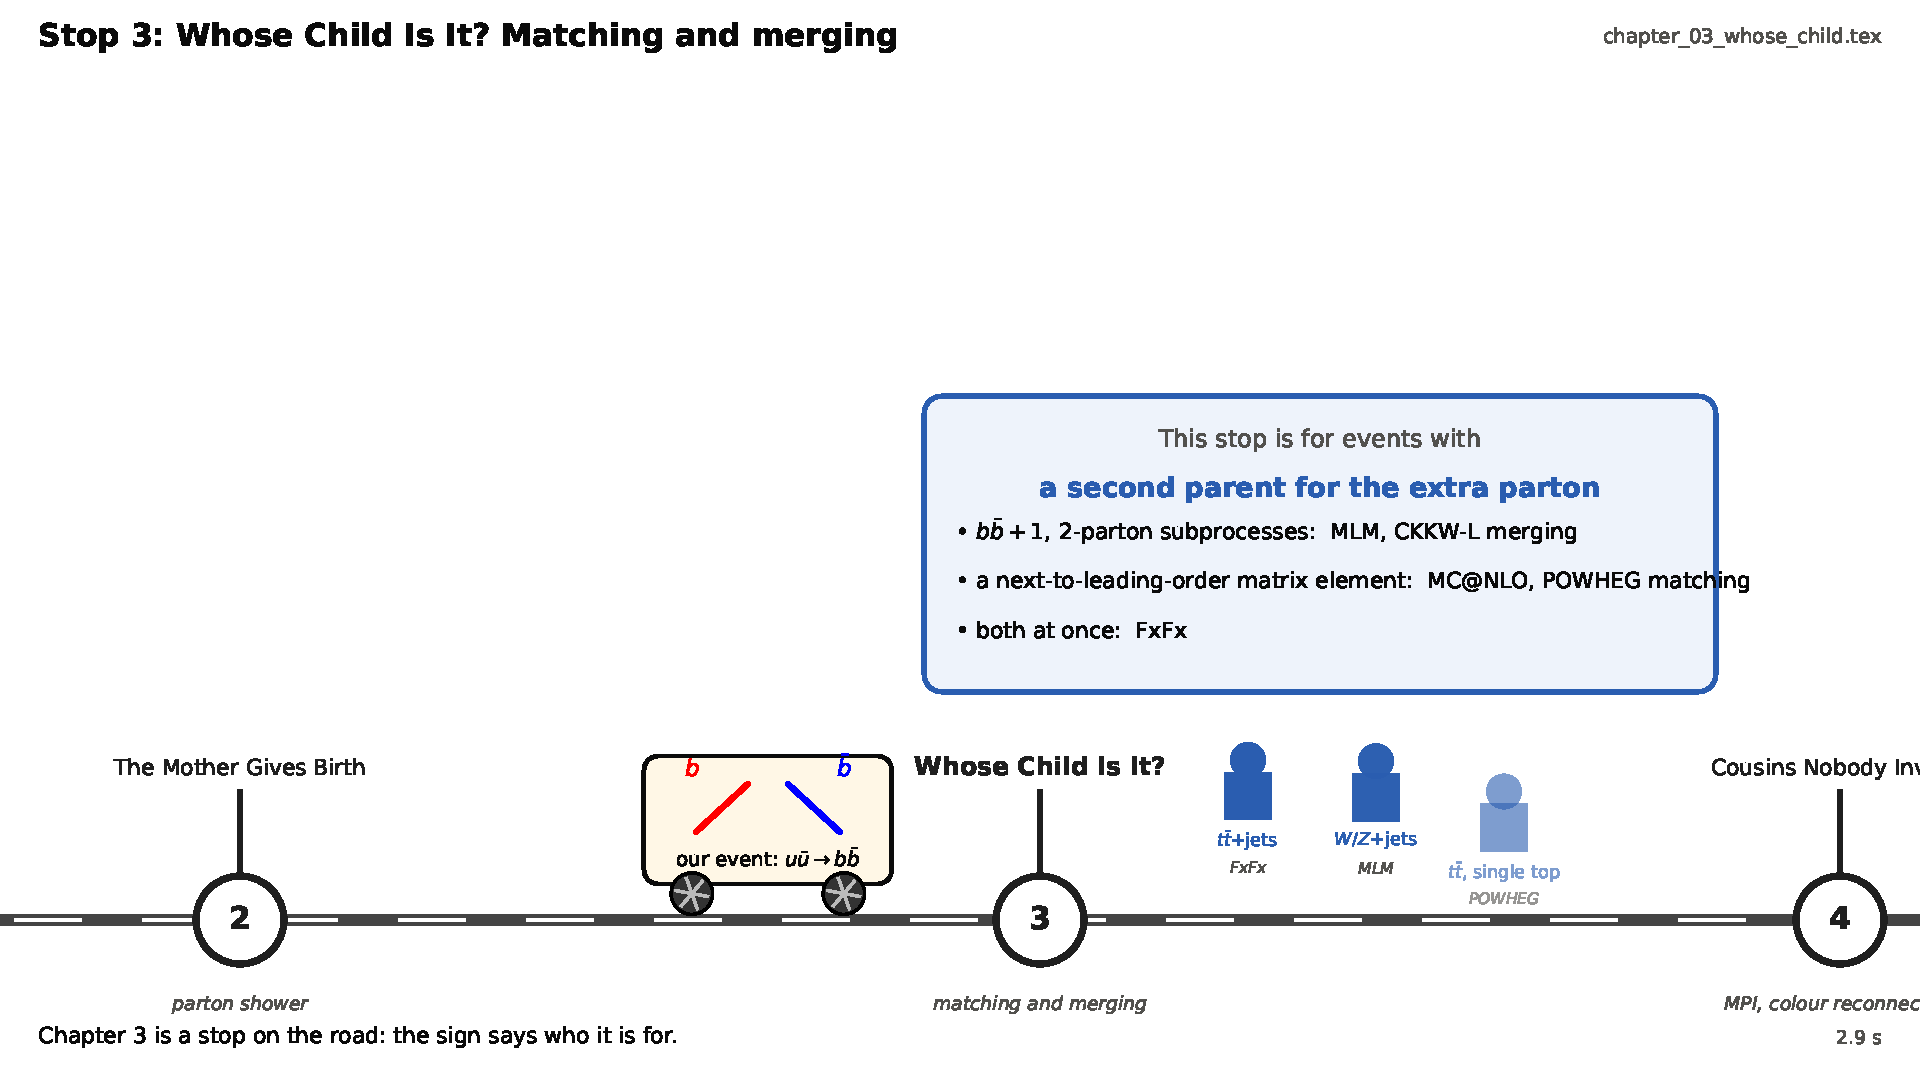
\includegraphics[page=1,width=0.325\textwidth]{MnM/animate_whose_child_stills.pdf}\hfill
\includegraphics[page=2,width=0.325\textwidth]{MnM/animate_whose_child_stills.pdf}\hfill
\includegraphics[page=3,width=0.325\textwidth]{MnM/animate_whose_child_stills.pdf}
\caption[Three frames of the film: the sign, the verdict, the next stop]{One frame per beat of the film, drawn by \file{animate\_whose\_child.py} with \code{--stills}. Left: the cart with our event arrives at stop 3 and the sign unfolds, naming the events this stop is for; the passengers of merged and matched samples get off. Middle: the card for our event, one $2\to2$ process with one parent for every extra parton, the stamp, and the ledger row that repeats itself. Right: the cart rolls on to chapter 4.}
\label{fig:whose_child:stills}
\end{figure}

\paragraph{Who owns the extra gluon?}
\label{sec:whose_child:who_owns}
Guess first: if we had included $u\bar u\to\bbbar g$ in \cref{ch:ancestral_home},
how many of the $38$ branchings of our event would it have produced?
\Cref{fig:whose_child:double_counting} gives the answer with the merging
scale CMS uses most often.

\begin{figure}[htbp]\centering
\resizebox{\textwidth}{!}{% ---------------------------------------------------------------------------
% Matching and merging in one picture. (a) The same final state, b bbar + one
% gluon, reached twice: by the 2->2 matrix element followed by one shower
% emission, and by the 2->3 matrix element. (b) The transverse-momentum axis
% of the extra parton with the two descriptions, the merging scale, and the
% branchings of OUR event (winners of the -v log of
% standalone_parton_showering.py, seed 1), none of which was ever at risk of
% being counted twice because the record has no 2->3 matrix element.
% ---------------------------------------------------------------------------
\begin{tikzpicture}[x=1cm,y=1cm,
  every node/.style={font=\footnotesize},
  fermion/.style={thick,postaction={decorate},decoration={markings,mark=at position 0.55 with {\arrow[scale=1.1]{Stealth}}}},
  antifermion/.style={thick,postaction={decorate},decoration={markings,mark=at position 0.45 with {\arrowreversed[scale=1.1]{Stealth}}}},
  gluon/.style={thick,decorate,decoration={coil,aspect=0,segment length=4pt,amplitude=1.8pt}},
  vertex/.style={fill=black,circle,inner sep=1.5pt},
  lab/.style={font=\scriptsize,align=center},
  head/.style={font=\small\bfseries},
  blob/.style={draw,fill=gray!25,circle,minimum size=7mm,inner sep=0pt},
  me/.style={fill=blue!10,draw=blue!60!black,rounded corners=2pt,inner sep=3pt,font=\scriptsize,align=center},
  ps/.style={fill=orange!15,draw=orange!70!black,rounded corners=2pt,inner sep=3pt,font=\scriptsize,align=center},
  tick/.style={very thick}]
% ---------------- (a) the same child, claimed twice ------------------------------------------------
\node[head,anchor=west] at (-0.3,3.3) {(a) one child, two parents};
% left: 2->2 ME + shower emission
\begin{scope}
\coordinate (V1) at (1.2,0.9); \coordinate (V2) at (2.9,0.9);
\draw[fermion] (0,2.0) -- (V1) node[pos=0,above left,lab] {$u$};
\draw[antifermion] (0,-0.2) -- (V1) node[pos=0,below left,lab] {$\bar u$};
\draw[gluon] (V1) -- (V2);
\coordinate (E) at (3.9,1.7);
\draw[fermion] (V2) -- (E); \draw[fermion] (E) -- (4.9,2.3) node[right,lab] {$b$};
\draw[gluon,orange!80!black] (E) -- (5.0,1.2) node[right,lab,text=orange!80!black] {$g$ (shower)};
\draw[antifermion] (V2) -- (4.9,-0.2) node[right,lab] {$\bar b$};
\node[vertex] at (V1) {}; \node[vertex] at (V2) {}; \node[vertex,fill=orange!80!black] at (E) {};
\node[me,anchor=north west] at (-0.2,-0.9) {$|\mathcal M_{2\to2}|^2$ \textbf{+} shower kernel\\$\dfrac{\alphas}{2\pi}\dfrac{\mathrm d\pt^2}{\pt^2}\,P_{qq}(z)$};
\node[lab,text=black!60] at (2.4,-2.6) {chapter 2: $113.32\GeV$ bounds the gluon};
\end{scope}
\node[font=\large] at (6.9,0.9) {$\neq$};
% right: 2->3 ME
\begin{scope}[xshift=8.2cm]
\coordinate (V1) at (1.2,0.9); \coordinate (V2) at (2.9,0.9);
\draw[fermion] (0,2.0) -- (V1) node[pos=0,above left,lab] {$u$};
\draw[antifermion] (0,-0.2) -- (V1) node[pos=0,below left,lab] {$\bar u$};
\draw[gluon] (V1) -- (V2);
\coordinate (E) at (3.9,1.7);
\draw[fermion] (V2) -- (E); \draw[fermion] (E) -- (4.9,2.3) node[right,lab] {$b$};
\draw[gluon,blue!60!black] (E) -- (5.0,1.2) node[right,lab,text=blue!60!black] {$g$ (matrix element)};
\draw[antifermion] (V2) -- (4.9,-0.2) node[right,lab] {$\bar b$};
\node[vertex] at (V1) {}; \node[vertex] at (V2) {}; \node[vertex,fill=blue!60!black] at (E) {};
\node[lab,text=black!60,anchor=north west] at (-0.2,-1.0) {+ the gluon from the $\bar b$, from the\\initial state, and all interferences};
\node[me,anchor=north west] at (-0.2,-1.9) {$|\mathcal M_{2\to3}|^2$: exact at tree level,\\ singular as $\pt\to0$, no Sudakov};
\end{scope}
% ---------------- (b) the pT axis of the extra parton ---------------------------------------------
\begin{scope}[yshift=-7.2cm]
\node[head,anchor=west] at (-0.3,3.5) {(b) the merging scale divides the \pt of the extra parton, and where our event's branchings fall};
% axis: log-ish, 0.5 .. 130 GeV mapped to 0..14 cm by hand
\draw[-{Stealth},thick] (0,0) -- (14.6,0) node[right,lab] {$\pt$ of the extra parton};
\foreach \x/\l in {0.4/1,3.3/3,5.4/10,8.1/30,10.9/100} {\draw (\x,0.1) -- (\x,-0.1); \node[lab,below] at (\x,-0.1) {$\l\GeV$};}
% regions
\fill[orange!15] (0,1.5) rectangle (8.1,2.5);
\fill[blue!10] (8.1,1.5) rectangle (11.5,2.5);
\node[ps,draw=none,fill=none] at (4.0,2.0) {\textbf{shower territory}: $\pt<Q_{\mathrm{cut}}$\\Sudakov-resummed, many soft and collinear partons};
\node[me,draw=none,fill=none] at (9.8,2.0) {\textbf{matrix-element territory}\\$\pt>Q_{\mathrm{cut}}$: exact, wide angle};
\draw[dashed,thick,red!70!black] (8.1,-0.3) -- (8.1,2.7);
\node[lab,text=red!70!black,anchor=east] at (8.0,2.9) {merging scale $Q_{\mathrm{cut}}\simeq30\GeV$ (CMS FxFx)};
\draw[dashed,thick,black!60] (11.5,-0.3) -- (11.5,2.7);
\node[lab,text=black!60,anchor=west] at (11.6,2.9) {$\pt^{\max}=113.3\GeV$: chapter 2's wall};
% our event's branchings: ISR 53.9 51.4 42.2 (orange, above axis), FSR 34.2 32.1 25.6 22.1 13.4 10.6 (red), then many below 6
\foreach \x in {9.5,9.4,8.9} {\draw[tick,green!50!black] (\x,0.0) -- (\x,0.6);}
\foreach \x in {8.4,8.2,7.7,7.3,6.1,5.6} {\draw[tick,red!70!black] (\x,0.0) -- (\x,0.6);}
\foreach \x in {4.1,4.0,3.9,3.4,2.5,2.4,2.2,1.9,1.8,1.5,1.2,1.0,0.9,0.7,0.6,0.5,0.4} {\draw[tick,gray] (\x,0.0) -- (\x,0.4);}
\node[lab,text=green!50!black,anchor=south west] at (8.8,0.65) {ISR 53.9, 51.4, 42.2};
\node[lab,text=red!70!black,anchor=south] at (6.5,0.65) {FSR 34.2 ($\bar b$), 32.1 ($b$),\\25.6, 22.1, 13.4, 10.6};
\node[lab,text=gray,anchor=south] at (2.3,0.45) {29 more, all below $6\GeV$};
\node[lab,text=black!65,text width=14.4cm,anchor=north west] at (-0.3,-0.7) {Ticks: the 38 winning branchings of our event, from the \code{-v} log of chapter 2. In a merged sample the five hardest would have been produced by a $2\to3$ or $2\to4$ matrix element and the shower would have been \emph{forbidden} to emit above $Q_{\mathrm{cut}}$; here the shower produced all of them, which is exact only in the collinear and soft limits. For a single $b$ jet of $\pt\approx100\GeV$ the difference is a few percent of the family's momentum, well inside the seed-to-seed spread of $26\GeV$.};
\end{scope}
\end{tikzpicture}
}
\caption[The same gluon from two parents, and the merging scale against the branchings of our event]{(a) The same $\bbbar g$ final state reached by the $2\to2$ matrix element followed by one shower emission, and by the $2\to3$ matrix element; summing them counts the gluon twice. (b) The transverse momentum of the extra parton with the two territories separated by the merging scale, and the $38$ winning branchings of our event from the \code{-v} log of \cref{ch:mother_gives_birth}: five lie above a merging scale of $30\GeV$ and would, in a merged sample, have come from a matrix element.}
\label{fig:whose_child:double_counting}
\end{figure}

The arithmetic of the problem fits in one line. With $\mathcal P(\pt)$ the
shower's probability of an emission at \pt from the Born configuration,
$\Delta$ its Sudakov factor and $\sigma_1$ the $2\to3$ cross section with the
extra parton above \pt, the two descriptions of the emission rate are
\begin{equation}
  \frac{\mathrm d\sigma}{\mathrm d\pt}\bigg|_{\mathrm{shower}}
   = \sigma_0\,\Delta(\pt^{\max},\pt)\,\mathcal P(\pt),
  \qquad
  \frac{\mathrm d\sigma}{\mathrm d\pt}\bigg|_{\mathrm{ME}}
   = \frac{\mathrm d\sigma_1}{\mathrm d\pt},
  \qquad
  \mathcal P(\pt)\xrightarrow{\ \pt\to0\ }\frac{1}{\sigma_0}\frac{\mathrm d\sigma_1}{\mathrm d\pt}.
  \label{eq:whose_child:two_rates}
\end{equation}
The last limit is the whole story: at small \pt the matrix element and the
shower kernel agree, so the shower's Sudakov factor is the right thing to
keep there; at large \pt they differ, the matrix element is right and the
shower has no business emitting. Every recipe of
\cref{sec:whose_child:recipes} is a way of drawing the line between the
two, at a \emph{merging scale} $Q_{\mathrm{cut}}$, so that the sum is
neither double counted nor discontinuous. For our event the shower emitted
on both sides of the line: three initial-state branchings at $53.9$, $51.4$
and $42.2\GeV$ and the twins' first gluons at $34.2$ and $32.1\GeV$ would
have been the matrix element's children in a merged sample with
$Q_{\mathrm{cut}}=30\GeV$, the remaining $33$, all below $26\GeV$ and
$29$ of them below $6\GeV$, the shower's. \PYTHIA's own answer for a plain
$2\to2$ QCD process is cruder than any merging: it either stops the shower
at the factorisation scale, the ``wall'' of \cref{eq:mother_gives_birth:ptmax}
(the default behaviour of \code{pTmaxMatch} for a final state of quarks,
which \CMSSW leaves untouched), or lets it run to the kinematic
limit with a damping factor that mimics the matrix element on average, the
``power shower'' of \cite{Plehn:2005cq,Corke:2010zj}. The exact
matrix-element corrections \PYTHIA does apply, following
\cite{Miu:1998ju,Norrbin:2000uu}, cover colour-singlet production and
resonance decays, not a coloured $2\to2$ final state like ours.

\paragraph{The recipes, one paragraph each.}
\label{sec:whose_child:recipes}
Three families of recipes draw that line, and \cref{fig:whose_child:recipes}
shows them as flow charts before each gets its paragraph.

\begin{figure}[htbp]\centering
\resizebox{\textwidth}{!}{% ---------------------------------------------------------------------------
% The three families of recipes as flow charts: (a) tree-level merging of jet
% multiplicities (MLM and CKKW-L), (b) NLO matching of one multiplicity
% (MC@NLO and POWHEG), (c) FxFx = (a) applied to (b). Nothing in this figure
% is used for our event; it is the map of what the official samples do.
% ---------------------------------------------------------------------------
\begin{tikzpicture}[x=1cm,y=1cm,
  every node/.style={font=\footnotesize},
  box/.style={draw,rounded corners=2pt,inner sep=4pt,align=center,font=\scriptsize,minimum width=2.6cm},
  me/.style={box,fill=blue!10,draw=blue!60!black},
  ps/.style={box,fill=orange!15,draw=orange!70!black},
  dec/.style={box,fill=red!8,draw=red!60!black},
  result/.style={box,fill=green!10,draw=green!50!black},
  flow/.style={-{Stealth[length=2mm]},thick},
  head/.style={font=\small\bfseries},
  lab/.style={font=\scriptsize,align=center}]
% ---------------- (a) tree-level merging ---------------------------------------------------------
\node[head,anchor=west] at (0,5.4) {(a) tree-level merging (MLM, CKKW-L): several multiplicities, one sample};
\node[me] (me0) at (1.4,4.2) {$u\bar u\to\bbbar$\\$+0$ partons};
\node[me] (me1) at (4.7,4.2) {$u\bar u\to\bbbar g$\\$+1$ parton, $\kt>\code{xqcut}$};
\node[me] (me2) at (8.4,4.2) {$u\bar u\to\bbbar gg,\ \bbbar q\bar q$\\$+2$ partons};
\node[ps] (sh) at (4.6,2.7) {shower each event with the emission\\ scale bounded by the parton it already has};
\node[dec] (mlm) at (3.5,1.3) {MLM: cluster the showered partons into \kt jets at \code{qcut};\\ keep the event only if every ME parton has its own jet\\ (and the highest multiplicity may have extra jets)};
\node[dec] (ckkw) at (11.2,1.3) {CKKW-L: reweight by the Sudakov factors\\ of the shower history the ME would have had,\\ veto shower emissions above $Q_{\mathrm{cut}}$};
\node[result] (out) at (7.6,-0.3) {one sample, exact wide-angle jets above $Q_{\mathrm{cut}}$,\\ resummed below, smooth across the scale};
\draw[flow] (me0) -- (sh); \draw[flow] (me1) -- (sh); \draw[flow] (me2) -- (sh);
\draw[flow] (sh) -- (mlm); \draw[flow] (sh) -- (ckkw);
\draw[flow] (mlm) -- (out); \draw[flow] (ckkw) -- (out);
\node[lab,anchor=west,text=black!60] at (10.5,4.2) {$\sigma_n\propto\alphas^{\,n}$: each extra\\ leg costs a power of $\alphas$,\\ cut off by \code{xqcut} to stay finite};
% ---------------- (b) NLO matching ---------------------------------------------------------------
\begin{scope}[yshift=-7.2cm]
\node[head,anchor=west] at (0,5.4) {(b) NLO matching (MC@NLO, POWHEG)};
\node[me] (born) at (1.6,4.2) {Born $u\bar u\to\bbbar$\\ $+$ one-loop virtual};
\node[me] (real) at (5.1,4.2) {real emission\\ $u\bar u\to\bbbar g$, $ug\to\bbbar u$, \dots};
\node[dec] (sub) at (3.1,2.7) {subtract from the real emission what the shower's\\ first emission would generate anyway (MC@NLO),\\ or generate the hardest emission with the exact\\ real matrix element and let the shower fill in below (POWHEG)};
\node[result] (outb) at (3.1,1.0) {NLO cross section and NLO shape of the first emission;\\ MC@NLO events may carry negative weights, POWHEG's do not};
\draw[flow] (born) -- (sub); \draw[flow] (real) -- (sub); \draw[flow] (sub) -- (outb);
% ---------------- (c) FxFx ---------------------------------------------------------------
\node[head,anchor=west] at (8.6,5.4) {(c) FxFx = (a) on top of (b)};
\node[me] (f0) at (9.6,4.2) {$\bbbar+0$ at NLO};
\node[me] (f1) at (12.6,4.2) {$\bbbar+1$ at NLO};
\node[dec] (fx) at (11.1,2.7) {MC@NLO each, then MLM-style\\ jet matching at $Q_{\mathrm{cut}}$ with\\ Sudakov reweighting between them};
\node[result] (outc) at (11.1,1.0) {NLO accuracy for the 0- and 1-jet rates\\ in one sample (CMS: $\ttbar$, $W/Z$+jets)};
\draw[flow] (f0) -- (fx); \draw[flow] (f1) -- (fx); \draw[flow] (fx) -- (outc);
\end{scope}
\end{tikzpicture}
}
\caption[Tree-level merging, NLO matching and FxFx as flow charts]{The three families of recipes. (a) Tree-level merging combines samples of different parton multiplicities, each cut off by \code{xqcut}, and decides after the shower whether an event is kept (MLM) or how it is weighted (CKKW-L). (b) NLO matching corrects one multiplicity by one order, either by subtracting the shower's first emission from the real-emission matrix element (MC@NLO) or by generating the hardest emission exactly and showering below it (POWHEG). (c) FxFx applies (a) to samples made with (b). None of them touches our event.}
\label{fig:whose_child:recipes}
\end{figure}

\paragraph{Tree-level merging: MLM.} Generate $\bbbar+0$, $+1$, $+2$ partons
at tree level, each with the extra partons separated by more than
\code{xqcut} in \kt so that the $2\to3$ cross section is finite; shower
each event; cluster the showered partons into \kt jets at a scale
\code{qcut} $>$ \code{xqcut}; keep the event only if every matrix-element
parton is matched to its own jet, and for the highest multiplicity also if
there are extra, softer jets. Events in which the shower produced a jet
above \code{qcut} that the matrix element did not are rejected, which is how
the double counting is removed and how the Sudakov suppression of the
matrix-element legs is applied, event by event rather than as a
weight~\cite{Mangano:2006rw,Alwall:2007fs}. In \PYTHIA the step is
\code{JetMatching:scheme = 1} with \code{JetMatching:qCut} and
\code{JetMatching:nJetMax}; CMS uses it for its \MG multijet, Drell--Yan and
$W$+jets leading-order samples with \code{qcut} between $19$ and $30\GeV$.

\paragraph{Tree-level merging: CKKW and CKKW-L.} Instead of rejecting events,
reconstruct for each matrix-element configuration the shower history that
would have produced it, weight the event by the Sudakov factors and
coupling ratios of that history, and veto shower emissions above the
merging scale~\cite{Catani:2001cc}. L\"onnblad's version uses the
shower's own Sudakov factors, obtained by trial showers, so that the
weights are exactly what the shower would have given~\cite{Lonnblad:2001iq,Lonnblad:2011xx};
the unitarised form UMEPS makes the merged inclusive cross section equal
to the lowest-multiplicity one~\cite{Lonnblad:2012ng}, and Sherpa's
implementation with truncated showers is~\cite{Hoeche:2009rj}. All these
are sub-percent-level different for well-separated jets and differ mainly
in how smooth the result is across $Q_{\mathrm{cut}}$.

\paragraph{NLO matching: MC@NLO and POWHEG.} Both raise one multiplicity to
next-to-leading order, which fixes the normalisation to $\sim10\%$
(\cref{sec:ancestral_home:scales}) and gives the hardest emission
its exact shape. MC@NLO subtracts from the real-emission matrix element the
term the shower's first emission generates, so that the sum is NLO without
double counting; the subtraction can be larger than the term, and a fraction
of the events, typically $10$--$30\%$, carries negative
weight~\cite{Frixione:2002ik,Alwall:2014hca}. POWHEG instead generates the
hardest emission with the exact real matrix element and a Sudakov built from
it, then hands the event to a shower restricted below that emission's
scale; the weights are positive but the shower must respect the
\code{SCALUP} bound, which for \PYTHIA's \pt-ordered shower is only
approximately the same variable~\cite{Nason:2004rx,Frixione:2007vw}. CMS's
inclusive $\ttbar$ and single-top samples are POWHEG.

\paragraph{FxFx and the NLO mergings.} FxFx is MLM applied to MC@NLO
samples of different multiplicities, with the Sudakov reweighting between
them done consistently at NLO~\cite{Frederix:2012ps,Frederix:2015eii}; in
\PYTHIA it is \code{JetMatching:doFxFx = on} with \code{JetMatching:qCut}
and \code{JetMatching:nQmatch}, and CMS uses it with $Q_{\mathrm{cut}}=30\GeV$
for $\ttbar$+jets and $W/Z$+jets, where the measurement of
\cite{CMS:2022ilp} compares it with the MLM and other predictions jet by
jet. MEPS@NLO~\cite{Hoeche:2012yf} and UNLOPS~\cite{Lonnblad:2012ix} are the
CKKW-type counterparts; MiNLO and MiNNLO$_{\mathrm{PS}}$
\cite{Hamilton:2012np,Monni:2019whf} reach the same goal from the POWHEG
side and, for colour-singlet production, at NNLO. The review
\cite{Buckley:2011ms} and the \PYTHIA guide \cite{Bierlich:2022pfr},
chapter on matching and merging, are the places to read all of this at
length.

\paragraph{Our jet at this stage: nothing changes, by construction.}
\label{sec:whose_child:our_jet}
The ledger receives a row that repeats the previous one
(\cref{tab:whose_child:ledger}). It is there so that the chain of stages is
complete, and as a reminder that for a merged sample this row would be the
first in which the matrix element, not the shower, decided whether the
mother's $32\GeV$ gluon exists. What little there is to run at this stop,
the film, the two shower experiments of the exercises and the settings of
the official recipes, is in the companion of this chapter,
\begin{center}
  \companion{chapter_03_MnM}
\end{center}

\begin{table}[htbp]\centering
\caption[Energy ledger at the stage ``Whose Child Is It?'']{Energy ledger at
the stage ``Whose Child Is It?''. $\Delta\pt$ is relative to the previous
row; no matching or merging is applied to our event, so the row is copied.}
\label{tab:whose_child:ledger}
\begin{tabular}{lrrrr}\toprule
Stage & $\pt$ [GeV] & $m$ [GeV] & $n_{\mathrm{const}}$ & $\Delta\pt$ [GeV] \\ \midrule
\ledgerrow{$b$ family after the shower ($\dR<0.4$)}{100.45}{13.52}{3}{--}
\ledgerrow{$b$ family after matching and merging (none applied)}{100.45}{13.52}{3}{$0$}
\bottomrule
\end{tabular}
\end{table}

\section{What this stop is, and what it is not}
\label{sec:whose_child:caveats}

It is a map of a road we do not take, and the reason is worth stating
plainly rather than hiding. Our event is one leading-order process,
\code{HardQCD:qqbar2bbbar}, with no additional subprocess
($u\bar u\to\bbbar g$, $ug\to\bbbar u$, \dots) anywhere in the sample, neither
in the standalone script, nor in the \CMSSW configuration of
\cref{sec:ancestral_home:validation}, nor in the \MG run of
\cref{sec:ancestral_home:madgraph}, which produced $\bbbar$ and nothing
else. There is exactly one parent for every extra parton, the shower, and
nothing to match it to. The price is the one named in
\cref{sec:mother_gives_birth:caveats}: wide-angle emissions above the
starting scale of $113.32\GeV$ are forbidden and those below it are only
logarithmically accurate. For following one $b$ jet of $100\GeV$ through
the detector that price is small, a few percent of the family's momentum
against a seed-to-seed spread of $26\GeV$, and the official CMS QCD
multijet samples made with \PYTHIA alone pay it too. It is \emph{not} small
when the extra jets are the measurement, $\ttbar$+jets, $W/Z$+jets or the
multijet background of a search, and that is where the recipes of
\cref{sec:whose_child:recipes} are used. Three things this stop is not:
\begin{itemize}[nosep]
  \item It is not a correction that was skipped. Nothing is missing from a
    \code{HardQCD} sample except the physics it never claimed, hard
    wide-angle jets.
  \item It is not a statement that the shower's hard emissions are right.
    Five of the $38$ branchings of our event lie above a merging scale of
    $30\GeV$ and would, in a merged sample, have come from a matrix element
    with a different \pt and angular distribution; which of the two is
    closer to nature at $\pt\approx100\GeV$ is Exercise~1.
  \item It is not a stage of the event. No particle is added, moved or
    removed here, the record of \cref{ch:mother_gives_birth} is the record
    of \cref{ch:uninvited_cousins}, and the ledger row is a copy.
\end{itemize}

\section{Further reading}
\label{sec:whose_child:further_reading}
MLM matching is defined in \cite{Mangano:2006rw} and compared with CKKW,
CKKW-L and others in \cite{Alwall:2007fs}; CKKW is \cite{Catani:2001cc},
its dipole-shower form \cite{Lonnblad:2001iq,Lonnblad:2011xx}; MC@NLO is
\cite{Frixione:2002ik}, POWHEG \cite{Nason:2004rx,Frixione:2007vw}, FxFx
\cite{Frederix:2012ps}. The \MG paper \cite{Alwall:2014hca} documents the
settings CMS writes into its gridpacks, and \cite{Buckley:2011ms} is the
general review.

\begin{pitfalls}
\begin{itemize}[nosep]
  \item \textbf{No merging is not an error for our sample.} A \PYTHIA
    \code{HardQCD} sample is a leading-order $2\to2$ sample showered up to
    its factorisation scale; nothing is missing from it except the physics
    it never claimed, hard wide-angle jets. Do not add \code{JetMatching}
    settings to a sample that has no matrix-element partons to match.
  \item \textbf{\code{qcut} must exceed \code{xqcut}, and both are physics.}
    Changing \code{qcut} by a factor two changes the one-jet rate of an MLM
    sample by several percent; the variation is a systematic uncertainty
    in CMS analyses, not a tuning knob.
  \item \textbf{Negative weights are not a bug.} An MC@NLO or FxFx sample
    with $20\%$ negative weights needs $(1-2\times0.2)^{-2}\approx3$ times
    the events for the same statistical power, and every histogram must be
    filled with the sign of \code{genWeight}.
  \item \textbf{Merged samples are not to be compared by jet counts to
    unmerged ones.} The ``third jet'' of a dijet event in a \PYTHIA
    \code{HardQCD} sample is the shower's; in a merged sample it is a
    matrix-element jet above $Q_{\mathrm{cut}}$. The two agree at low \pt
    and differ at high \pt and wide angle, by construction.
\end{itemize}
\end{pitfalls}

\begin{exercises}
\item The standalone shower can be told to start at the kinematic limit
  instead of the factorisation scale: run
  \code{standalone\_parton\_showering.py --ptmax 396 --repeat 2000} and
  compare the branching counts and the family \pt of
  \cref{tab:mother_gives_birth:numbers}, which \code{--history} writes per
  shower to a \file{.stats.json}, with the default run. This
  is the undamped power shower; which of the two is closer to what a
  $2\to3$ matrix element would give at $\pt\approx100\GeV$, and why?
\item The \code{--history} JSON of a single shower lists its branchings:
  loop over \code{--seed} $1$ to $300$ and count the showers in
  which at least one branching has $\pt>30\GeV$. This fraction is the share
  of events that an FxFx sample with $Q_{\mathrm{cut}}=30\GeV$ would have
  taken from the $\bbbar+1$-parton matrix element rather than from the
  shower.
\item Open a CMS \MG+\PYTHIA fragment for Drell--Yan with FxFx (the
  \code{DYJetsToLL\_M-50\_TuneCP5\_13TeV-amcatnloFXFX-pythia8} dataset) and
  identify \code{JetMatching:qCut}, \code{JetMatching:nJetMax} and
  \code{JetMatching:nQmatch}. Why is \code{nQmatch} five for Drell--Yan and
  what would it have to be for our $\bbbar$ process?
\end{exercises}

\subsection*{Open problems in the context of Phase-2 LHC}
\label{sec:whose_child:open_problems}

The matching and merging of the Run-2 samples was designed for a few
hundred fb$^{-1}$; the $3000\,\mathrm{fb}^{-1}$ of the High-Luminosity
LHC and the multiplicities of its jets strain it in three
ways~\cite{Azzi:2019yne,HSFPhysicsEventGeneratorWG:2020gxw}.
\begin{enumerate}
  \item \textbf{Negative weights and the event budget.} At $20$--$30\%$
    negative weights an NLO-matched sample costs several times the
    simulation of a positive-weight one, and the detector simulation, not
    the generator, is the expensive step. Reweighting the subtraction
    \cite{Frederix:2020trv}, resampling \cite{Andersen:2020sjs} and
    positive-weight matching schemes \cite{Danziger:2021xvr} each trade
    some accuracy for statistical power; which trade is acceptable for a
    Phase-2 $\ttbar$+jets sample is an open question of the HSF generator
    working group.
  \item \textbf{The merging scale as a systematic.} The merging-scale
    dependence of $V$+jets predictions at high jet multiplicity, studied for
    the HL-LHC in \cite{Hoche:2019flt} and across generators in the Les
    Houches comparisons \cite{Amoroso:2020lgh}, is of the same size as the
    experimental precision Phase-2 will reach. Sector showers
    \cite{Brooks:2020mab} and the logarithmically accurate showers of
    \cref{sec:mother_gives_birth:open_problems} promise merged predictions
    whose $Q_{\mathrm{cut}}$ dependence is a genuine higher-order effect
    rather than a shower artefact; none is yet in a CMS production sample.
  \item \textbf{Matching and the heavy-quark mass.} The interpretation of
    the top mass measured from jets depends on how the matched hardest
    emission and the shower treat the quark's mass
    \cite{Nason:2017cxd,Hoang:2020iah}; the same question exists for the
    $b$ quark of our event and its dead cone
    (\cref{sec:mother_gives_birth:dead_cone}). Extending NNLO matching
    \cite{Monni:2019whf} from colour singlets to heavy-quark pairs, and
    deciding what mass the shower should carry, is where a Phase-2
    precision top and $b$-jet programme meets this chapter.
\end{enumerate}

%% ---------------------------------------------------------------------------
% Chapter 4: Cousins Nobody Invited: Underlying Event and Colour Reconnection
% The scripts, records, logs and films of this stop live in example/MPI/, and
% the technical companion of the chapter is chapter/chapter_04_MPI.md: how to
% run the scripts, how to read the records and logs, how the official numbers
% were obtained, and the full tables. The book gives the physics.
% ---------------------------------------------------------------------------
%% chapter-local shorthands (\pt already carries a subscript, so it cannot take another)
\providecommand{\ptzero}{\ensuremath{p_{\mathrm{T}0}}\xspace}
\providecommand{\sigint}{\ensuremath{\sigma_{\mathrm{int}}}\xspace}
\providecommand{\signd}{\ensuremath{\sigma_{\mathrm{ND}}}\xspace}
\providecommand{\bmean}{\ensuremath{\langle b\rangle}\xspace}
\chapter{Cousins Nobody Invited: Underlying Event and Colour Reconnection}
\chaptermark{Cousins Nobody Invited}
\label{ch:uninvited_cousins}

\begin{journeybox}
The rest of the two protons does not stay at home. Other partons scatter softly,
beam remnants hadronise, and colour strings reconnect across the event. Distant
cousins join the road and some of their energy ends up inside our jet.
\end{journeybox}

\physicsline{the divergent QCD $2\to2$ cross section and its regularisation,
multiparton interactions as a Poisson process in impact parameter, the
overlap of two protons and the enhancement factor, the chain of interactions
below the hard scale, depleted parton densities and companion quarks, beam
remnants and primordial transverse momentum, the MPI-based colour
reconnection and the string length, the transverse-region definition of the
underlying event, the CP5 tune, the underlying-event energy inside a cone.
The one number to take away: at this collision geometry the uninvited
cousins add $1.6\pm2.2\GeV$ to a cone of $\dR<0.4$ around the mother, and
in our event they happened to add nothing.}

\section{What we will see at this stop}
\label{sec:uninvited_cousins:what_we_compute}

At the end of \cref{ch:mother_gives_birth} the record contained forty
partons and a hole. The two incoming partons of \file{event_PS.lhe} carried
momentum fractions $x_A=0.017$ and $x_B=0.47$ and nothing balanced them;
the two protons that had supplied them were simply absent. That is not how
a collision ends. Each proton is a bag of partons, and when two bags pass
through each other the pair that produced our $\bbbar$ is only the hardest
of the pairs that scatter. The others scatter too, at lower transverse
momentum, each with its own small shower, and what is left of each proton,
the \emph{beam remnant}, flies on down the beam pipe carrying most of the
energy of the collision. Between all of them run colour strings, and the
strings do not respect which scattering a parton came from. This stop is
about the family that was already on the road when ours set out: the
cousins nobody invited.

The number to take away is small and it is the first entry in the ledger
that \emph{adds} to the mother's family rather than subtracting from it. In
our event, no parton from the rest of the protons happened to land within
$\dR<0.4$ of the $b$ quark, so the ledger row of the previous chapter
survives to the hundredth of a GeV; within $\dR<0.8$ the underlying event
adds $3.4\GeV$ and lifts the family mass from $13.5$ to $20.2\GeV$. On
average, over many dressings of the same hard event at the same collision
geometry, the $R=0.4$ cone receives $1.6\pm2.2\GeV$ and the $R=0.8$ cone
$5.9\pm4.4\GeV$. The uninvited cousins are a few percent of the jet at
$R=0.4$ and are the reason jets are not built with $R=1$; the detector will
later add two hundred \emph{other} collisions on top
(\cref{ch:crowd_on_the_road}), and the methods of
\cref{ch:paying_for_uninvited} will have to tell the two apart. As at the
previous stops we meet the number four times, from the top down: a film
shows two protons overlapping, the chain of secondary scatterings running
down in \pt, the remnants being formed, the strings reconnecting and the
same hard event dressed four hundred times; a Python file takes the
showered record of \cref{ch:mother_gives_birth} and adds the multiparton
interactions, the beam remnants and the colour reconnection in two seconds,
following \PYTHIA's construction class by class; the theory derives why the
QCD $2\to2$ cross section must exceed the proton--proton cross section, how
the impact parameter enters, how the chain is generated, what the protons
look like after each scattering, how the remnants are formed and what
colour reconnection does to the strings; and the official packages, the
real \PYTHIA dressing the same hard event two thousand times and the CMS
generator job of \cref{ch:ancestral_home}, get the last word.

\MG again does not appear: multiparton interactions, remnants and colour
reconnection are \PYTHIA's job in every CMS sample, whatever produced the
hard process.

\paragraph{The film.}
\label{sec:uninvited_cousins:animation}
The film first: the fourth on the playlist of \jitjetworld replays the
seed-1 dressing at the \CMSSW impact parameter in five narrated scenes,
once without and once with colour reconnection, so that every number on the
screen, and every number the narrator says, is produced by the classes that
wrote the record. Two discs of matter slide towards each other in the
transverse plane while the overlap and the enhancement factor rise along
their curves, until the collision stops at the impact parameter of the
\CMSSW event; a scale runs from the hard scale down to the cut-off and the
ladder of the $24$ secondary scatterings fills rung by rung, fifteen of
them crowded below $2\GeV$; the momentum bars of the two protons are eaten
interaction by interaction until the grey remnant partons appear with their
flavours and their primordial kicks; the colour strings of the event are
drawn before and after reconnection, the $b$ quark's own string
highlighted among the $33$ that remain; and the same showered event is
dressed with seeds $1,2,3,\ldots$ while the running means settle next to
the \PYTHIA values. \Cref{fig:uninvited_cousins:stills} shows the first
four scenes; the fifth is \cref{tab:uninvited_cousins:numbers} in motion.
Watch first, and let the formulae catch up.

\begin{figure}[htbp]\centering
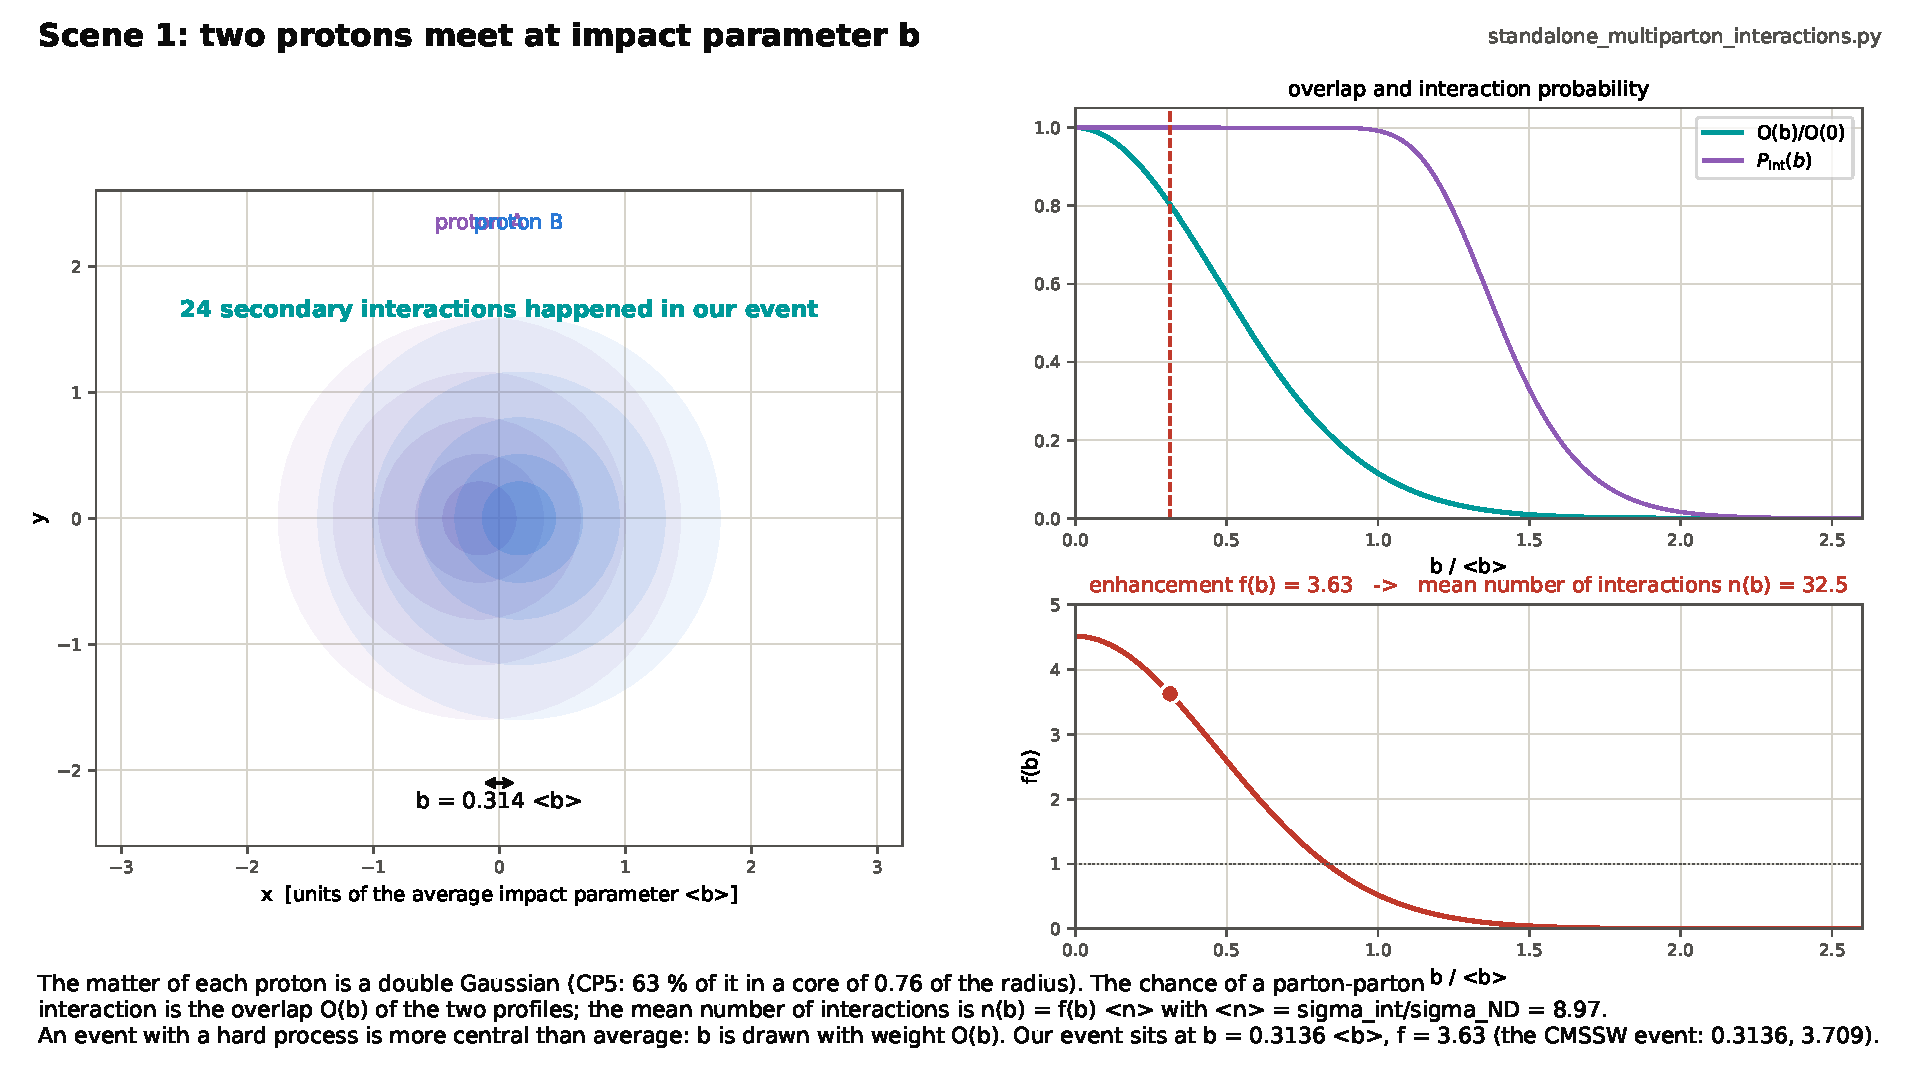
\includegraphics[page=1,width=0.47\textwidth]{MPI/Standalone/animate_standalone_multiparton_interactions_stills.pdf}\hfill
\includegraphics[page=2,width=0.47\textwidth]{MPI/Standalone/animate_standalone_multiparton_interactions_stills.pdf}\\[2mm]
\includegraphics[page=3,width=0.47\textwidth]{MPI/Standalone/animate_standalone_multiparton_interactions_stills.pdf}\hfill
\includegraphics[page=4,width=0.47\textwidth]{MPI/Standalone/animate_standalone_multiparton_interactions_stills.pdf}
\caption[Key frames of the animated standalone MPI stage]{Key frames of
four of the five scenes of the animated standalone MPI stage, drawn by
\file{animate_standalone_multiparton_interactions.py} with \code{--stills}.
Top left: the two protons at impact parameter $b$ with the overlap and the
enhancement factor. Top right: the \pt ladder of the 24 secondary
scatterings, the $(\eta,\phi)$ picture and the no-interaction probability.
Bottom left: the momentum bars of the two protons being used up and the
primordial-$k_{\mathrm{T}}$ kicks. Bottom right: the colour strings before
and after reconnection and the string length. The fifth scene, four hundred
dressings of the same event against the \PYTHIA reference, is the table of
this section. The film itself is the fourth on the playlist of
\jitjetworld.}
\label{fig:uninvited_cousins:stills}
\end{figure}

\paragraph{The picture to carry.}
\Cref{fig:uninvited_cousins:two_protons_sketch} is the stop in one sketch:
one proton--proton collision contains many parton--parton scatterings, in
our event the hard one at $113\GeV$ and $24$ softer ones between $11.5$
and $0.43\GeV$, because the parton--parton cross section, regularised at
small \pt by the finite size of the proton, is nine times the cross section
for the two protons to interact at all. Everything else at this stop, the
impact parameter, the chain, the depleted protons, the remnants and the
strings, follows from reading that ratio as a count.

\begin{figure}[htbp]\centering
\resizebox{\textwidth}{!}{% ---------------------------------------------------------------------------
% Why there is more than one scattering per collision. Left: the two protons
% of our event pass through each other; the hard u ubar -> b bbar scattering
% is one of many parton-parton scatterings, the others soft. Right: the
% parton-parton cross section dsigma/dpT^2 against pT, bare (1/pT^4, divergent)
% and regularised (1/(pT^2+pT0^2)^2); its integral above pTmin, sigma_int,
% exceeds the non-diffractive cross section, so <n> = sigma_int/sigma_ND
% scatterings happen per collision. Numbers from the -v log of
% standalone_multiparton_interactions.py (section "setting the scene").
% ---------------------------------------------------------------------------
\begin{tikzpicture}[x=1cm,y=1cm,
  every node/.style={font=\footnotesize},
  proton/.style={draw,very thick,fill=gray!10},
  parton/.style={circle,inner sep=0pt,minimum size=2mm},
  hard/.style={line width=1.8pt,red!80!black},
  soft/.style={line width=0.9pt,teal!80!black},
  lab/.style={font=\scriptsize,align=center},
  head/.style={font=\small\bfseries},
  gluon/.style={thick,decorate,decoration={coil,aspect=0,segment length=3pt,amplitude=1.2pt},gray!70}]
% ---------------- (a) one collision, many scatterings ------------------------------------------
\node[head,anchor=west] at (-3.4,3.2) {(a) one collision, 25 parton--parton scatterings};
\node[proton,ellipse,minimum width=46mm,minimum height=30mm] (A) at (-1.4,0) {};
\node[proton,ellipse,minimum width=46mm,minimum height=30mm,fill=gray!14] (B) at (1.4,0.6) {};
\node[lab,anchor=east] at (-3.9,0) {proton A\\$+z$};
\node[lab,anchor=west] at (3.9,0.6) {proton B\\$-z$};
\draw[-{Stealth[length=2mm]},gray!70,thick] (-4.6,-1.6) -- (-3.4,-1.6) node[midway,below,font=\scriptsize] {$6800\GeV$};
\draw[-{Stealth[length=2mm]},gray!70,thick] (4.6,2.2) -- (3.4,2.2) node[midway,above,font=\scriptsize] {$6800\GeV$};
% the hard scattering: u ubar -> b bbar
\coordinate (H) at (0.0,0.3);
\draw[hard] (-2.4,-0.3) -- (H) node[pos=0.35,below,font=\scriptsize,text=red!80!black] {$\bar u$, $x=0.0022$};
\draw[hard] (2.4,0.9) -- (H) node[pos=0.35,above,font=\scriptsize,text=red!80!black] {$u$, $x=0.39$};
\draw[hard,-{Stealth[length=2.2mm]}] (H) -- (1.6,-1.7) node[right,font=\scriptsize,text=red!80!black] {$b$, $113\GeV$};
\draw[hard,-{Stealth[length=2.2mm]}] (H) -- (-1.6,2.3) node[left,font=\scriptsize,text=red!80!black] {$\bar b$};
\node[circle,fill=red!80!black,inner sep=1.6pt] at (H) {};
% the soft scatterings (24 of them): drawn as small crosses with short outgoing legs
\foreach \px/\py/\ang in {-1.1/0.9/20, -0.6/-0.7/-35, 0.7/1.3/60, 0.9/-0.4/-70, -0.2/1.6/15, 0.3/-1.1/40, 1.5/0.2/-20, -1.6/0.1/70, -0.5/0.5/-55, 1.1/0.9/35, 0.0/-0.3/80, -1.0/-1.1/10}
  {\node[circle,fill=teal!80!black,inner sep=1.1pt] at (\px,\py) {};
   \draw[soft,-{Stealth[length=1.4mm]}] (\px,\py) -- ++(\ang:0.55);
   \draw[soft,-{Stealth[length=1.4mm]}] (\px,\py) -- ++(\ang+180:0.55);}
\node[lab,text=teal!80!black,anchor=north] at (0.0,-2.0) {24 secondary scatterings, $\pt$ from $11.5$ down to $0.43\GeV$,\\each with its own shower, drawn from the depleted protons};
\node[lab,text=black!65,anchor=north] at (0.0,-2.8) {what is left of each proton becomes the beam remnants};
% ---------------- (b) the cross section and its regulator --------------------------------------
\begin{scope}[xshift=9.0cm,yshift=-2.6cm]
\node[head,anchor=west] at (-0.3,5.8) {(b) the cross section must be tamed};
\draw[-{Stealth}] (0,0) -- (6.4,0) node[below left=2pt and -2pt] {$\pt$};
\draw[-{Stealth}] (0,0) -- (0,5.2) node[above,align=center,font=\scriptsize] {$\mathrm{d}\sigma/\mathrm{d}\pt^2$};
\foreach \x/\l in {1.5/$p_{\mathrm{T}0}$,3.0/$2p_{\mathrm{T}0}$,4.5/$3p_{\mathrm{T}0}$} {\draw (\x,0) -- (\x,-0.1) node[below] {\l};}
\draw[dashed,red!70!black] (1.5,0) -- (1.5,4.6);
\node[font=\scriptsize,text=red!70!black,anchor=west] at (1.55,4.75) {$p_{\mathrm{T}0}=1.44\GeV$ (CP5 at $13.6\TeV$)};
% bare: 4.5/x^4 in units of pT0 -> x = pT/pT0, plotted from where it enters the frame
\begin{scope}
\clip (0.05,0) rectangle (6.3,4.6);
\draw[very thick,dashed,gray!70!black] plot[domain=0.95:4.2,samples=120,variable=\t] ({1.5*\t},{4.5/(\t*\t*\t*\t)});
\draw[very thick,teal!80!black] plot[domain=0.05:4.2,samples=160,variable=\t] ({1.5*\t},{4.5/((\t*\t+1)*(\t*\t+1))});
\fill[teal!80!black,opacity=0.12] plot[domain=0.13:4.2,samples=120,variable=\t] ({1.5*\t},{4.5/((\t*\t+1)*(\t*\t+1))}) -- (6.3,0) -- (0.2,0) -- cycle;
\end{scope}
\node[font=\scriptsize,text=gray!70!black,anchor=west,align=left] at (2.3,3.9) {bare: $\alphas^2(\pt^2)/\pt^4$\\diverges, $\sigma_{\mathrm{int}}\to\infty$};
\node[font=\scriptsize,text=teal!80!black,anchor=west,align=left] at (2.3,2.6) {regularised: $\dfrac{\alphas^2(\pt^2+p_{\mathrm{T}0}^2)}{(\pt^2+p_{\mathrm{T}0}^2)^2}$\\colour screening below $p_{\mathrm{T}0}$};
\draw[dotted,black!60] (0.2,0) -- (0.2,4.4);
\node[font=\scriptsize,anchor=south,rotate=90] at (0.08,2.0) {$\pt^{\min}=0.2\GeV$};
\node[font=\scriptsize,text=teal!80!black,anchor=north west,align=left] at (0.35,1.5) {shaded: $\sigma_{\mathrm{int}}=497\,\mathrm{mb}$\\$\sigma_{\mathrm{ND}}=55.4\,\mathrm{mb}$\\$\langle n\rangle=\sigma_{\mathrm{int}}/\sigma_{\mathrm{ND}}=9.0$};
\end{scope}
\end{tikzpicture}
}
\caption[One collision, many scatterings, and the regularised cross
section]{Left: one proton--proton collision contains many parton--parton
scatterings; in our event the hard $\bar uu\to\bbbar$ at $113\GeV$ and 24
softer ones between $11.5$ and $0.43\GeV$. Right: the parton--parton cross
section $\mathrm{d}\sigma/\mathrm{d}\pt^2$ diverges as $1/\pt^4$ (dashed)
and is regularised by the replacement of \cref{eq:uninvited_cousins:regularised}
(solid); its integral above $\pt^{\min}$, shaded, is nine times the
non-diffractive cross section.}
\label{fig:uninvited_cousins:two_protons_sketch}
\end{figure}

\paragraph{A picture to carry: the other tenants.} The project picture of
\cref{ch:mother_gives_birth} had two main contractors and their
subcontractors. This chapter adds the rest of the building. The hard process
rented the top floor; the other floors are rented too, by tenants who never
heard of our project, each running a small project of their own with the
same rules, the same subcontracting, the same recoils. They share the
building's budget (the protons' momentum), so every tenant that moves in
leaves less for the next, and the landlord (the remnant) keeps what nobody
rented. Then the electricians come: the colour strings that hadronisation
will pull into hadrons do not run floor by floor but are rewired so that
the total length of cable is as short as possible, and a cable that starts
on our floor may now end on somebody else's. The picture captures the three
things the chapter derives: more than one scattering per collision, a
shared and depleted budget, and strings that cross system boundaries. Its
limit is the same as before: the scatterings are independent only in the
model's leading approximation, and the model has knobs, the tune, which
the data fix.

\paragraph{The number, three ways.}
\label{sec:uninvited_cousins:validation}
\label{sec:uninvited_cousins:standalone_code}
\Cref{tab:uninvited_cousins:numbers} gives away the ending, with the same
warning as \cref{tab:mother_gives_birth:numbers} and one more. The stage is
random, so single events are compared on structure and ensembles on
averages. The new warning is the \emph{impact parameter}: the first thing
the model draws is how centrally the two protons hit, and nothing in the
hard process fixes it. Seed~1 of the standalone script, left to itself,
draws a peripheral collision with a single secondary scattering, which would
make a dull chapter; the \CMSSW event of \cref{ch:ancestral_home} happened to
be central, $b=0.31\bmean$, with 31 secondary scatterings. The book's record
therefore fixes the impact parameter to the \CMSSW value, so that the two
can be compared at the same geometry, and every ensemble below is given both
ways: with $b$ drawn, as nature does it, and at $b=0.3136\bmean$.

The standalone script is a port of four classes of \PYTHIA~8,
\code{MultipartonInteractions}, \code{BeamParticle}, \code{BeamRemnants} and
the \code{reconnectMPIs} model of \code{ColourReconnection}, into Python
that needs NumPy and SciPy and nothing else; it imports the shower of
\cref{ch:mother_gives_birth} and runs it on every secondary system. Its
learning mode, \code{-v}, prints the regularised cross section with its
integral, the overlap table, the state of the two protons after the hard
process, and then every secondary interaction with its scale, its veto
weight, the depleted densities it saw, the channel it chose and the size of
its shower, every remnant with its flavour and kick, and every colour
reconnection decision; the $1500$ lines for seed~1 at the \CMSSW impact
parameter are committed, and every number quoted in the theory of this
chapter is taken from that log.
\label{sec:uninvited_cousins:pythia}

The first official check is \PYTHIA itself, dressing the same hard event
two thousand times with the CP5 settings of the \CMSSW configuration,
showers, multiparton interactions, remnants and colour reconnection on,
hadronisation off; since the impact parameter cannot be fixed from the
Python binding, the fixed-$b$ column keeps the \PYTHIA events within a
narrow window around the \CMSSW value. Read the columns as before. The
geometry agrees as far as four hundred dressings can tell: the means of $b$
and $f$ differ by $3\%$ and $7\%$ with a statistical error of $3\%$ each,
and $f(0.3136)$ is $2\%$ low because the script normalises the enhancement
factor differently from \PYTHIA (\cref{sec:uninvited_cousins:caveats}). The remnant count, the hardest secondary scattering and the
underlying-event density agree at the $5$--$10\%$ level, and the extra \pt
inside the cones follows the density. The one real disagreement is the
number of scatterings, $20\%$ low in the standalone chain at both
geometries, and its cause is known: \PYTHIA interleaves the multiparton
interactions with the initial- and final-state showers of \emph{all}
systems in one common \pt sequence, so that the depletion a scattering sees
is only that of the scatterings and emissions harder than itself, while
the script showers each system to its cut-off before drawing the next,
softer scattering, which makes the proton look emptier than it should.
Without any showering the two chains agree to $4\%$; the remaining
difference, a $10\%$ stronger soft radiation of the chapter-2 shower, was
already seen in \cref{sec:mother_gives_birth:pythia}. The cone \emph{mass}
is not compared: the standalone ensembles keep the seed-1 shower, whose
family mass of $13.5\GeV$ is a high draw, while \PYTHIA reshowers to
$8\GeV$ on average.
\label{sec:uninvited_cousins:cmssw}

The second official check is the \code{GEN} step of
\cref{sec:ancestral_home:cmssw} with the parton level complete: the showers
of \cref{ch:mother_gives_birth} and, new at this stop, the multiparton
interactions, the remnants and colour reconnection, the hadron level still
off. Its log prints the same numbers the script derives, the regularised cross section integrated at
initialisation, ``\code{pT0 = 1.44 gives sigmaInteraction = 500.67 mb}'',
and for the first event ``\code{Impact parameter b = 3.136e-01 gives
enhancement factor = 3.709}'' and ``\code{Number of MPI = 32}'', the hard
process counted among them. The book's record was fixed to that impact
parameter, and \cref{sec:uninvited_cousins:our_jet_at_this_stage_ue_energy_inside_r}
reads the \CMSSW event next to the standalone one. How each column was
produced, the commands, the options, the logs and the status codes, is in
the companion of this chapter,
\begin{center}
  \companion{chapter_04_MPI}
\end{center}
together with the full tables behind every number quoted below.

\begin{table}[htbp]\centering\small
\caption[The rest of the protons obtained three ways]{The rest of the
protons obtained three ways. ``Secondary'' means not belonging to the hard
$\bbbar$ system and its shower; ``UE'' (underlying event) means the partons
of the secondary systems and the remnants; cones are drawn around the final
copy of the $b$ quark. The first four columns are averages over $2000$
(\PYTHIA), $400$ (standalone), $537$ (\PYTHIA at fixed $b$) and $400$
dressings of the same showered event, the spread of a single event after
$\pm$; the fifth is the one dressing with seed~1 at $b=0.3136\bmean$ that
wrote \file{example/MPI/event_MPI.lhe}; the last is the single \CMSSW event.
The standalone ensembles keep the seed-1 shower of
\cref{ch:mother_gives_birth} and redraw only this stage; \PYTHIA redraws
everything.}
\label{tab:uninvited_cousins:numbers}
\scriptsize\setlength{\tabcolsep}{3.5pt}
\begin{tabular}{lrrrrrr}\toprule
 & \PYTHIA & standalone & \PYTHIA & standalone & standalone & \CMSSW \\
 & $b$ drawn & $b$ drawn & $b=0.3136$ & $b=0.3136$ & seed 1 & 1 event \\ \midrule
interactions, incl.\ the hard one & $18.0\pm9.9$ & $14.7\pm7.2$ & $27.5\pm5.4$ & $21.4\pm4.2$ & $25$ & $32$ \\
$b/\bmean$, $f(b)$ & $0.61$, $2.26$ & $0.63$, $2.10$ & $0.31$, $3.70$ & $0.31$, $3.63$ & $0.31$, $3.63$ & $0.31$, $3.71$ \\
final partons & $125\pm60$ & $138\pm54$ & $181\pm34$ & $190\pm33$ & $211$ & $169$ \\
\quad of which from secondary systems & $92$ & $88$ & $145$ & $137$ & $155$ & $142$ \\
\quad of which beam remnants & $10.2$ & $9.4$ & $13.6$ & $12.8$ & $16$ & $13$ \\
$\sum\pt$ of the secondary partons [GeV] & $134$ & $124$ & $212$ & $196$ & $230$ & $208$ \\
hardest secondary interaction [GeV] & $6.8$ & $6.5$ & $8.6$ & $8.4$ & $11.45$ & $6.65$ \\ \midrule
transverse UE density [GeV per unit $\eta$--$\phi$] & $2.21\pm1.72$ & $2.00\pm1.59$ & $3.48\pm1.54$ & $3.23\pm1.44$ & $2.10$ & -- \\
UE $\sum\pt$ within $\dR<0.4$ of the $b$ [GeV] & $1.21\pm2.48$ & $0.85\pm1.30$ & $1.80\pm2.43$ & $1.60\pm2.19$ & $0.00$ & $6.91$ \\
UE $\sum\pt$ within $\dR<0.8$ of the $b$ [GeV] & $4.57\pm5.20$ & $3.95\pm4.05$ & $7.32\pm5.68$ & $5.90\pm4.42$ & $3.61$ & -- \\
UE partons within $\dR<0.4$ / $0.8$ & $0.75$ / $2.99$ & $0.72$ / $2.87$ & $1.20$ / $4.75$ & $1.08$ / $4.20$ & $0$ / $3$ & $3$ / -- \\ \midrule
systems merged by colour reconnection & -- & $13.2$ & -- & $19.7$ & $23$ & -- \\
string length $\lambda$ before $\to$ after & -- & $563\to375$ & -- & $769\to472$ & $880\to521$ & -- \\
\bottomrule
\end{tabular}
\end{table}

\section{Let us dive into the details: the theory}
\label{sec:uninvited_cousins:theory}

\subsection{The rest of the protons does not stay quiet: multiparton interactions}
\label{sec:uninvited_cousins:the_rest_of_the_protons_does_not_stay_qu}

\subsubsection{A cross section larger than the proton: the regularised \texorpdfstring{$2\to2$}{2 to 2} rate}
\label{sec:uninvited_cousins:cross_section}

Guess first. \Cref{ch:ancestral_home} computed the cross section for
$\pthat>100\GeV$ of our process, $345\pb$. What is the cross section for
\emph{any} QCD $2\to2$ scattering with $\pthat>2\GeV$? The matrix elements
of \cref{sec:ancestral_home:cmssw} fall as $1/\pthat^4$ and the parton
densities rise steeply at small $x$, so the answer is enormous: with the
numbers of this chapter, $168\,\mathrm{mb}$, that is $1.7\times10^{11}\pb$,
and above $0.2\GeV$ it is $497\,\mathrm{mb}$. The total proton--proton cross
section at $13.6\TeV$ is $100\,\mathrm{mb}$, and the part of it that is not
elastic or diffractive, the non-diffractive cross section \signd, is
$55\,\mathrm{mb}$. A parton-level cross section ten times larger than the
cross section for the two protons to interact at all is not a
contradiction; it is a count. If each non-diffractive collision contains on
average $\langle n\rangle$ parton--parton scatterings above the cut, then
\begin{equation}
  \langle n\rangle=\frac{\sigint(\pt>\pt^{\min})}{\signd},
  \label{eq:uninvited_cousins:nmean}
\end{equation}
and the parton-level number, correctly read, says that an average collision
at the LHC contains \emph{nine} scatterings above $0.2\GeV$, not one. This
is the observation of Sj\"ostrand and van~Zijl~\cite{Sjostrand:1987su} on
which every \PYTHIA event rests, and it has a corollary that the rest of the
section makes precise: our hard scattering is accompanied by the others,
which do not know about it.

The count cannot be left to diverge, though, and the $1/\pt^4$ of the
matrix element does diverge as $\pt\to0$. Physically the divergence is cut
off by the finite size of the proton: a gluon of wavelength longer than the
distance between colour charges does not resolve them and is screened. The
model implements the screening by a single scale \ptzero,
\begin{equation}
  \frac{\mathrm{d}\hat\sigma}{\mathrm{d}\pt^2}\propto
  \frac{\alphas^2(\pt^2)}{\pt^4}
  \quad\longrightarrow\quad
  \frac{\alphas^2(\pt^2+\ptzero^2)}{(\pt^2+\ptzero^2)^2},
  \qquad
  \ptzero(E_{\mathrm{cm}})=\ptzero^{\mathrm{ref}}\left(\frac{E_{\mathrm{cm}}}{7\TeV}\right)^{\epsilon},
  \label{eq:uninvited_cousins:regularised}
\end{equation}
applied to every $2\to2$ channel of \cref{ch:ancestral_home} plus the
heavy-flavour channels $gg,q\bar q\to c\bar c,\bbbar$ with massive
kinematics. The regulator grows slowly with energy, because the proton is
resolved at smaller $x$ where the gluon density is higher and the screening
stronger; the two numbers $\ptzero^{\mathrm{ref}}$ and $\epsilon$ are the
most important parameters of any tune, and CP5~\cite{CMS:2019csb} sets them
to $1.41\GeV$ and $0.03344$. The full differential cross section summed over
channels and integrated over the rapidities of the two outgoing partons is
\begin{equation}
  \frac{\mathrm{d}\sigma}{\mathrm{d}\pt^2}=\sum_{i,j}\int\mathrm{d}y_3\,\mathrm{d}y_4\;
  x_1f_i(x_1,Q^2)\,x_2f_j(x_2,Q^2)\;\frac{\mathrm{d}\hat\sigma_{ij}}{\mathrm{d}\hat t}
  \Big|_{\mathrm{regularised}},\qquad
  x_{1,2}=\frac{\pt}{E_{\mathrm{cm}}}\left(e^{\pm y_3}+e^{\pm y_4}\right),
  \label{eq:uninvited_cousins:dsigma}
\end{equation}
with $Q^2=\pt^2$ in the densities (only the coupling takes the shifted
scale $\pt^2+\ptzero^2$, as in \PYTHIA), and
$\sigint=\int_{\pt^{\min}}\mathrm{d}\sigma$. Two details decide the number
and both cost me a day: a final state of two different partons is reached
twice when both rapidities run over their full range, once as the
$t$-channel and once as the $u$-channel configuration, so the sum must be
halved for those channels, exactly as \PYTHIA averages the two; and the
densities below the grid's lowest scale, $Q=1.65\GeV$, are frozen rather
than extrapolated, as \PYTHIA's own readers do, which matters because
scatterings below $2\GeV$ carry two thirds of \sigint.

\paragraph{The numbers.} The \code{-v} log opens with
$\ptzero=1.41\times(13600/7000)^{0.03344}=1.4417\GeV$ and
$\signd=100.309-21.89-23.0=55.42\,\mathrm{mb}$, the \CMSSW settings for the
total, elastic and diffractive cross sections at $13.6\TeV$, and then the
table of \cref{eq:uninvited_cousins:dsigma}:
\begin{center}\footnotesize
\begin{tabular}{rrrrr}\toprule
$\pt$ [GeV] & $\alphas(\pt^2+\ptzero^2)$ & $\bigl(\pt^2/(\pt^2+\ptzero^2)\bigr)^2$ & $\mathrm{d}\sigma/\mathrm{d}\pt^2$ [mb/GeV$^2$] & $\sigma(>\pt)$ [mb] \\ \midrule
$0.2$ & $0.370$ & $0.0004$ & $599$ & $497.3$ \\
$1.0$ & $0.330$ & $0.106$ & $100$ & $285.6$ \\
$1.442$ & $0.305$ & $0.250$ & $38.7$ & $217.9$ \\
$2.0$ & $0.278$ & $0.433$ & $20.9$ & $168.1$ \\
$5.0$ & $0.211$ & $0.852$ & $1.61$ & $33.95$ \\
$10.0$ & $0.178$ & $0.960$ & $0.0772$ & $5.17$ \\
$20.0$ & $0.153$ & $0.990$ & $0.00236$ & $0.561$ \\
$113.3$ & $0.114$ & $0.9997$ & $1.2\times10^{-7}$ & $0.00075$ \\
\bottomrule
\end{tabular}
\end{center}
The third column is the regulator's effect relative to the bare rate: at
$\pt=\ptzero$ one quarter, at $0.2\GeV$ four parts in ten thousand. The
integral, $\sigint=497.33\,\mathrm{mb}$, is what the \CMSSW log prints as
``\code{pT0 = 1.44 gives sigmaInteraction = 500.67 mb: accepted}'' at
initialisation, and $\langle n\rangle=497.33/55.42=8.97$. The cross section
above our hard scale, $0.75\,\mathrm{\mu b}$, is the last entry: a
$2\to2$ scattering above $113\GeV$ happens in one collision in $70\,000$,
which is why the hard process is always the first rung of the ladder and not
somewhere in the middle. The composition of the rate (panel~(c) of
\cref{fig:uninvited_cousins:cross_section_plot}) is gluon--gluon everywhere
below $10\GeV$: at the scale of our first secondary scattering the log
lists $gg\to gg$ with $65\%$ of the weight and the five next channels, all
quark--gluon, with $2$--$4\%$ each.

\begin{figure}[htbp]\centering
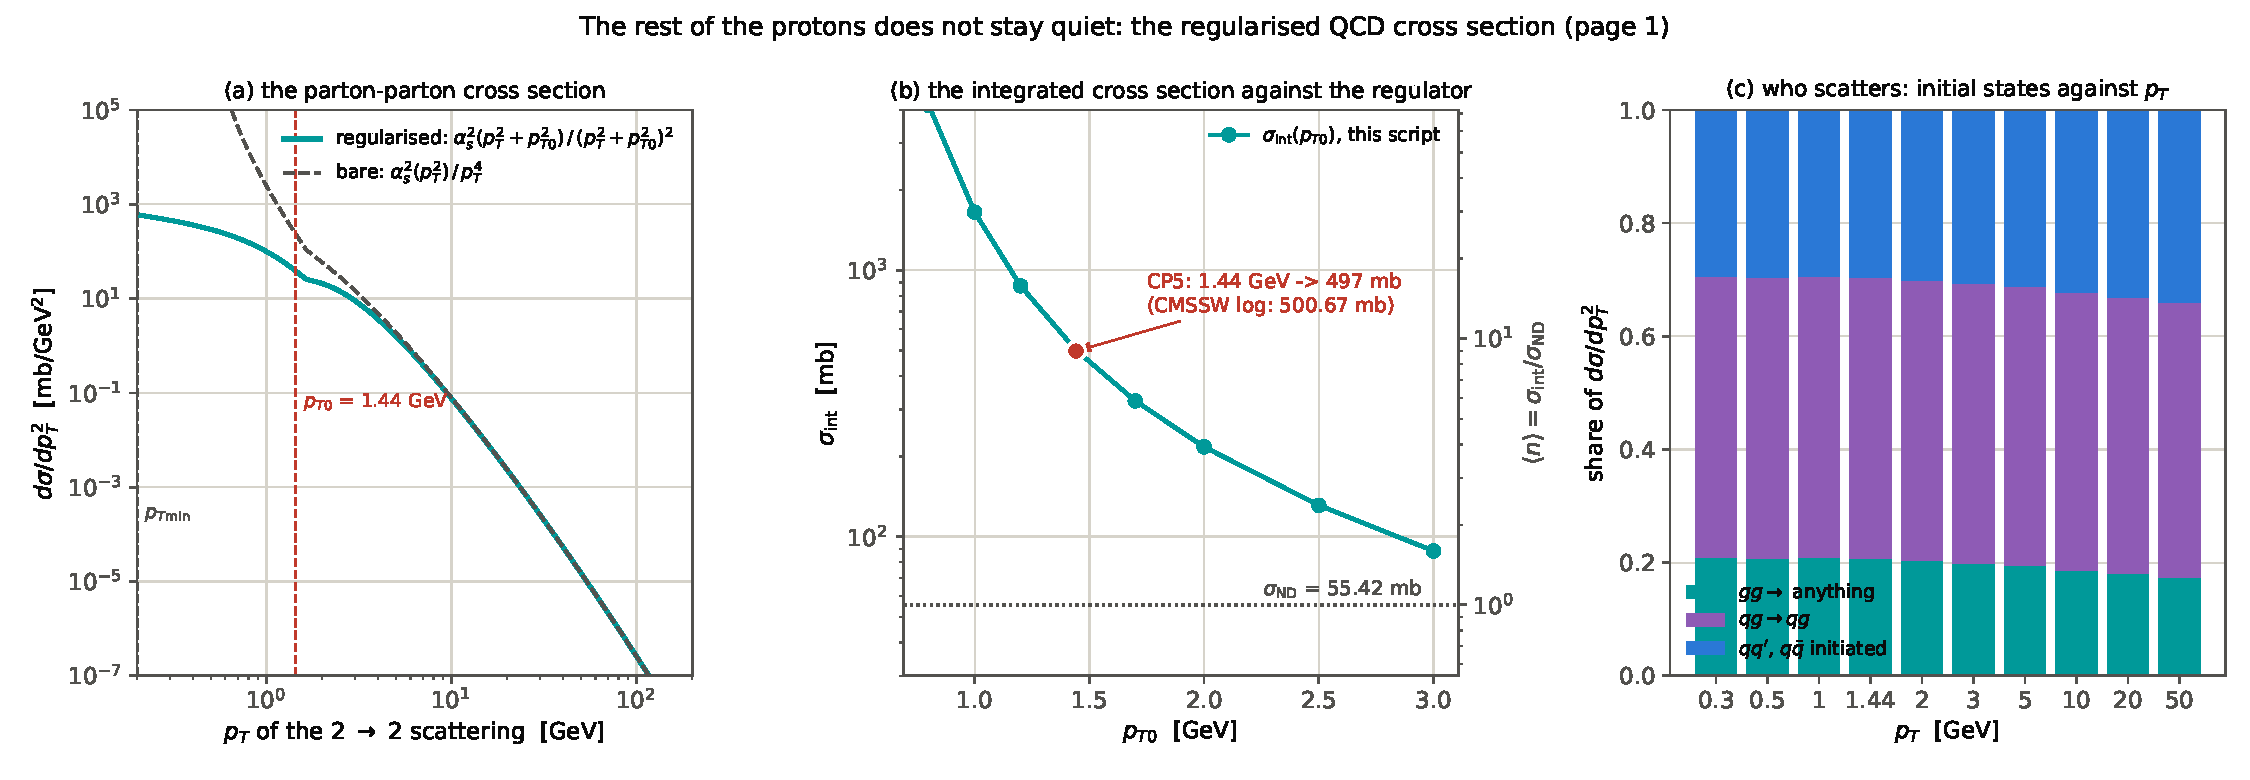
\includegraphics[page=1,width=\textwidth]{MPI/Standalone/theory_multiparton_interactions.pdf}
\caption[The regularised cross section and \sigint]{Page~1 of
\file{theory_multiparton_interactions.pdf}. (a) The bare and the regularised
parton--parton cross section of \cref{eq:uninvited_cousins:regularised}
against \pt, with \ptzero and $\pt^{\min}$ marked. (b) \sigint against the
regulator \ptzero, computed with the script's \code{SigmaInt} on a coarser
grid, the CP5 point against the \CMSSW log, and \signd as the horizontal
line; the right axis is $\langle n\rangle$. (c) The share of the rate from
$gg$, $qg$ and quark--quark initial states against \pt: gluons dominate
below $10\GeV$, where all the secondary scatterings of our event are.}
\label{fig:uninvited_cousins:cross_section_plot}
\end{figure}

\subsubsection{Where the two protons meet: the impact parameter}
\label{sec:uninvited_cousins:impact}

Guess again. Our hard scattering happened. Does that tell us anything about
how centrally the two protons hit? It does, and the direction is not
obvious: a hard scattering is more likely when more partons overlap, so the
collisions that contain one are more central than average, and a central
collision contains more of everything else as well. The number of
scatterings is therefore not Poisson with mean $\langle n\rangle$ in every
collision; it is Poisson with a mean that depends on the impact parameter,
$n(b)$, and the hard process biases $b$ towards zero. This is the second
ingredient of the model~\cite{Sjostrand:1987su}, and the one that makes the
spread in \cref{tab:uninvited_cousins:numbers} as large as it is.

\begin{figure}[htbp]\centering
\resizebox{\textwidth}{!}{% ---------------------------------------------------------------------------
% The impact parameter. Left: the two protons in the transverse plane, each a
% double-Gaussian matter distribution (CP5: 63 % of the matter in a core of
% 0.76 of the radius), displaced by b; the overlap O(b) is the hatched region.
% Right: the script's enhancement factor f(b) of the -v log ("the impact
% parameter" section; not PYTHIA's normalisation, see the chapter's caveats)
% with our event and the averages marked.
% ---------------------------------------------------------------------------
\begin{tikzpicture}[x=1cm,y=1cm,
  every node/.style={font=\footnotesize},
  lab/.style={font=\scriptsize,align=center},
  head/.style={font=\small\bfseries}]
% ---------------- (a) two protons in the transverse plane ----------------------------------
\node[head,anchor=west] at (-3.6,3.3) {(a) two protons meet at impact parameter $b$};
\coordinate (CA) at (-1.0,0);
\coordinate (CB) at (0.7,0.45);
% halo + core of each proton (double Gaussian): drawn as concentric discs
\foreach \c/\col in {CA/blue,CB/orange} {
  \fill[\col!15] (\c) circle (2.2);
  \fill[\col!30] (\c) circle (1.45);
  \fill[\col!45] (\c) circle (0.85);}
\begin{scope}
\clip (CA) circle (1.45);
\fill[pattern=north east lines,pattern color=black!70] (CB) circle (1.45);
\end{scope}
\draw[very thick,blue!70!black] (CA) circle (2.2);
\draw[very thick,orange!80!black] (CB) circle (2.2);
\node[circle,fill=blue!70!black,inner sep=1.5pt] at (CA) {};
\node[circle,fill=orange!80!black,inner sep=1.5pt] at (CB) {};
\draw[{Stealth}-{Stealth},thick] (CA) -- (CB) node[midway,below right=-1pt,font=\scriptsize] {$b$};
\node[lab,text=blue!70!black] at (-2.6,-2.0) {proton A\\core $63\%$, radius $0.76\,a$};
\node[lab,text=orange!80!black] at (2.4,2.3) {proton B\\(the same)};
\node[lab] at (-0.15,0.2) {};
\node[lab,anchor=north] at (-0.2,-2.6) {hatched: the overlap $O(b)=\int\rho_A(\vec r)\,\rho_B(\vec r-\vec b)\,\mathrm{d}^2r$\\the number of scatterings is Poisson with mean $n(b)=k\,O(b)$};
% ---------------- (b) f(b) --------------------------------------------------------------------
\begin{scope}[xshift=7.4cm,yshift=-2.7cm]
\node[head,anchor=west] at (-0.3,6.0) {(b) the script's enhancement $f(b)$};
\draw[-{Stealth}] (0,0) -- (6.6,0) node[right] {$b/\langle b\rangle$};
\draw[-{Stealth}] (0,0) -- (0,5.4) node[above,font=\scriptsize] {$f(b)$};
\foreach \x/\l in {0/0,1.5/0.5,3/1,4.5/1.5,6/2} {\draw (\x,0) -- (\x,-0.1) node[below] {\l};}
\foreach \y/\l in {1.1/1,2.2/2,3.3/3,4.4/4} {\draw (0,\y) -- (-0.1,\y) node[left] {\l};}
% f(b) from the log: b/<b> 0 .25 .5 .75 1 1.25 1.5 2 -> 4.517 3.928 2.594 1.315 0.522 0.166 0.044 0.002
\draw[very thick,teal!80!black] plot[smooth] coordinates {(0,4.969) (0.75,4.321) (1.5,2.853) (2.25,1.447) (3.0,0.574) (3.75,0.183) (4.5,0.048) (6.0,0.002)};
\draw[dashed,red!80!black] (0.941,0) -- (0.941,3.99);
\node[circle,fill=red!80!black,inner sep=2pt] at (0.941,3.99) {};
\node[font=\scriptsize,text=red!80!black,anchor=west,align=left] at (1.05,4.3) {our event: $b=0.3136\,\langle b\rangle$\\$f=3.63$ (\CMSSW: $3.71$), $f\langle n\rangle=32.5$};
\draw[dotted,black!60] (0,2.44) -- (6.4,2.44) node[pos=0.98,above left,font=\scriptsize,text=black!65] {$\langle f\rangle_{\mathrm{hard}}=2.22$};
\draw[dotted,black!60] (0,1.07) -- (6.4,1.07) node[pos=0.45,above left,font=\scriptsize,text=black!65] {$\langle f\rangle_{\mathrm{ND}}=0.97$};
\node[font=\scriptsize,text=teal!80!black,anchor=south west] at (0.1,4.97) {$f(0)=4.52$};
\node[font=\scriptsize,anchor=north west,align=left,text=black!65,text width=3.0cm] at (3.3,2.05) {minimum bias weights $b$ by $P_{\mathrm{int}}(b)$; a hard process by $O(b)$: central collisions favoured};
\end{scope}
\end{tikzpicture}
}
\caption[Two protons at impact parameter $b$ and the enhancement
$f(b)$]{Left: the two protons of our event in the transverse plane, each a
double-Gaussian matter distribution, displaced by the impact parameter $b$;
the overlap $O(b)$ is hatched. Right: the enhancement factor $f(b)$ as the
script computes it, with our event at
$b=0.3136\bmean$, the average over hard events and the average over
minimum-bias events marked.}
\label{fig:uninvited_cousins:overlap_sketch}
\end{figure}

The proton is given a matter distribution; CP5 uses a double Gaussian with
$63\%$ of the matter in a core of radius $0.7634$ of the outer radius
(\code{coreFraction}, \code{coreRadius} in the \CMSSW settings table). The
overlap of two such protons displaced by $\vec b$ is the time-integrated
product of the densities,
\begin{equation}
  O(b)=\int\mathrm{d}t\,\mathrm{d}^3x\;\rho(\vec x)\,\rho(\vec x+\vec b+\vec v t)
  =\sum_{\text{core/halo pairs}}c_{ij}\,\frac{e^{-b^2/(a_i^2+a_j^2)}}{\pi(a_i^2+a_j^2)},
  \label{eq:uninvited_cousins:overlap}
\end{equation}
a sum of three Gaussians in $b$ for the double-Gaussian profile. The mean
number of scatterings at impact parameter $b$ is taken proportional to the
overlap, $n(b)=k\,O(b)$, the probability that the collision interacts at all
is $P_{\mathrm{int}}(b)=1-e^{-n(b)}$, and $k$ is fixed by requiring that the
average over interacting collisions reproduce \cref{eq:uninvited_cousins:nmean},
\begin{equation}
  \langle n\rangle=\frac{\int\mathrm{d}^2b\;n(b)}{\int\mathrm{d}^2b\;P_{\mathrm{int}}(b)}
  =\frac{\sigint}{\signd},
  \qquad
  f(b)\equiv\frac{O(b)}{\langle O\rangle_{\mathrm{int}}},
  \quad
  \langle O\rangle_{\mathrm{int}}=\frac{\int\mathrm{d}^2b'\,P_{\mathrm{int}}(b')\,O(b')}{\int\mathrm{d}^2b'\,P_{\mathrm{int}}(b')}.
  \label{eq:uninvited_cousins:fb}
\end{equation}
The denominator of the first expression is the geometric cross section for
interacting at all, which is \signd in these units. The enhancement factor
$f(b)$, the overlap in units of its average over interacting collisions, so
that $\langle f\rangle=1$ for minimum bias, is the number that multiplies
every rate in the rest of the chapter. This is \PYTHIA's definition, and it
is the one place where I guessed wrong and the script still does: it fixes
$k$ by $k\,\langle O\rangle_{\mathrm{int}}=\langle n\rangle$ instead of the
first condition and takes $f(b)=O(b)\int\mathrm{d}^2b'\,P_{\mathrm{int}}/\int\mathrm{d}^2b'\,O$,
the ratio $n(b)/\langle n\rangle$ of the original model. The two choices
nearly cancel and leave the script's $f$ two percent below \PYTHIA's at the
$b$ of our event (\cref{sec:uninvited_cousins:caveats}). Which
$b$ a collision has is then drawn with a weight that depends on what is
asked: for minimum bias $\propto P_{\mathrm{int}}(b)\,\mathrm{d}^2b$, for a
collision known to contain a hard scattering
$\propto O(b)\,\exp[-f(b)\,\sigma(>Q_{\mathrm{hard}})/\signd]\,\mathrm{d}^2b$,
the exponential being the probability that no \emph{other} scattering above
the hard scale happened, which for our event is $0.99996$ and does not
matter.

\paragraph{The numbers.} The log prints the overlap table with the script's
$k=93.0$ for $\langle n\rangle=8.974$ (\PYTHIA's condition gives $89.7$),
$\bmean_{\mathrm{ND}}=1.24$ in the profile's own units, and $f(0)=4.52$;
the last two columns are $1-e^{-kO}$ and $kO(b)$ with that $k$, while the
rate the chain uses is $f(b)\langle n\rangle=0.97\,kO(b)$:
\begin{center}\footnotesize
\begin{tabular}{rrrrr}\toprule
$b/\bmean$ & $O(b)$ & $f(b)$ & $P_{\mathrm{int}}(b)$ & $n(b)$ \\ \midrule
$0$ & $0.448$ & $4.52$ & $1.000$ & $41.7$ \\
$0.25$ & $0.390$ & $3.93$ & $1.000$ & $36.2$ \\
$0.50$ & $0.257$ & $2.59$ & $1.000$ & $23.9$ \\
$0.75$ & $0.130$ & $1.32$ & $1.000$ & $12.1$ \\
$1.00$ & $0.052$ & $0.52$ & $0.992$ & $4.8$ \\
$1.25$ & $0.017$ & $0.17$ & $0.784$ & $1.5$ \\
$1.50$ & $0.004$ & $0.04$ & $0.331$ & $0.4$ \\
$2.00$ & $0.0002$ & $0.002$ & $0.016$ & $0.02$ \\
\bottomrule
\end{tabular}
\end{center}
Averaged with the minimum-bias weight the script's $f$ gives $0.97$, with
the hard-process weight $2.22$; \PYTHIA's normalisation gives $1$ and
$2.26$, and \PYTHIA measures $2.26$ over its two thousand events. Our event
is at $b=0.3136\bmean$, where the script finds $f=3.627$; \PYTHIA's
normalisation gives $3.704$ with the script's \sigint and $3.709$ with the
$500.67\,\mathrm{mb}$ of the \CMSSW log, which is the value that log
prints. The record keeps the script's $3.627$: the expected number of
secondary scatterings is $f\langle n\rangle=32.5$ ($33.2$ with \PYTHIA's
$f$), and the \CMSSW event got $31$, the standalone dressing $24$. Seed~1
with $b$ drawn lands at $1.21\bmean$, $f=0.20$, $f\langle n\rangle=1.8$ and
one secondary scattering; nature's
events are spread over the whole of panel~(c) of
\cref{fig:uninvited_cousins:overlap_plot}, and that spread, not the
scattering process, is the first reason why the underlying event of two
events with identical hard processes can differ by a factor of ten.

\begin{figure}[htbp]\centering
\includegraphics[page=2,width=\textwidth]{MPI/Standalone/theory_multiparton_interactions.pdf}
\caption[The proton profile, the overlap and the impact-parameter
distributions]{Page~2 of \file{theory_multiparton_interactions.pdf}. (a) The
double-Gaussian matter density of CP5 against a single Gaussian. (b) The
overlap $O(b)$, the interaction probability $P_{\mathrm{int}}(b)$ and the
script's enhancement $f(b)$. (c) The distribution
of $b/\bmean$ for minimum-bias collisions and for collisions with a hard
process, the latter against the $400$ dressings with $b$ drawn and
against \PYTHIA; our event and the \CMSSW event are the vertical line.}
\label{fig:uninvited_cousins:overlap_plot}
\end{figure}

\subsubsection{The chain of interactions below the hard scale}
\label{sec:uninvited_cousins:chain}

How are the $n(b)$ scatterings generated? Not all at once. If every
scattering took its partons from the full proton, the momentum sum could be
violated; the scatterings must be ordered and each must see what the
previous ones have taken. \PYTHIA orders them in \pt, hardest first, exactly
as the shower orders its emissions, and generates the next one with the
same veto algorithm (\cref{sec:mother_gives_birth:veto}). The hard process
sits at the top; the probability density for the next scattering at
$\pt$, given that the previous one was at $\pt^{\mathrm{prev}}$ and none
happened in between, is
\begin{equation}
  \frac{\mathrm{d}P}{\mathrm{d}\pt^2}=\frac{f(b)}{\signd}\,\frac{\mathrm{d}\sigma}{\mathrm{d}\pt^2}\;
  \exp\!\left[-\frac{f(b)}{\signd}\int_{\pt^2}^{(\pt^{\mathrm{prev}})^2}\frac{\mathrm{d}\sigma}{\mathrm{d}\pt'^2}\,\mathrm{d}\pt'^2\right],
  \label{eq:uninvited_cousins:chain}
\end{equation}
the Sudakov form factor of \cref{eq:mother_gives_birth:sudakov} with the
emission rate replaced by the scattering rate per non-diffractive collision.
The chain stops when the next scale falls below $\pt^{\min}$. The
overestimate that the veto algorithm needs is the regulator itself: with
$g(\pt^2)=C/(\pt^2+\ptzero^2)^2\ge\mathrm{d}\sigma/\mathrm{d}\pt^2$ the
integral is elementary and the trial scale is
\begin{equation}
  \pt^2=\left[\frac{1}{(\pt^{\mathrm{prev}})^2+\ptzero^2}-\frac{\signd\ln R}{f(b)\,C}\right]^{-1}-\ptzero^2,
  \qquad R\in(0,1),
  \label{eq:uninvited_cousins:trial}
\end{equation}
accepted with probability $(\mathrm{d}\sigma/\mathrm{d}\pt^2)/g(\pt^2)$.
Once a scale is accepted the rapidities $y_3$, $y_4$ are drawn flat within
the kinematic limits, which fixes $x_1$, $x_2$ by
\cref{eq:uninvited_cousins:dsigma}, the flavours and the channel are
chosen according to their weights at that point, the colour flow of
\PYTHIA's process tables is attached, and the system is showered from its
own \pt downwards with the shower of \cref{ch:mother_gives_birth}, with one
difference: the backward evolution of each side now reads the
\emph{depleted} density of the next subsection.

\begin{figure}[htbp]\centering
\resizebox{\textwidth}{!}{% ---------------------------------------------------------------------------
% The chain of interactions of our event: a ladder in pT from the hard
% scale 113.3 GeV down to pTmin = 0.2 GeV, with the 24 secondary interactions
% of the -v log ("the chain of interactions" section) as rungs, and the
% no-interaction probability between rungs written as a Sudakov-like factor.
% The vertical position is log10(pT). Right: the first rung worked out.
% ---------------------------------------------------------------------------
\begin{tikzpicture}[x=1cm,y=1cm,
  every node/.style={font=\footnotesize},
  rung/.style={line width=1.4pt,teal!80!black},
  hardrung/.style={line width=2.2pt,red!80!black},
  lab/.style={font=\scriptsize,align=left},
  head/.style={font=\small\bfseries},
  numbox/.style={draw,rounded corners=3pt,thin,fill=blue!6,align=left,inner sep=4pt,text width=8.8cm,font=\scriptsize}]
% y(pT) = 2.3*(log10(pT) + 0.7): pTmin 0.2 -> 0, 1 GeV -> 1.61, 10 -> 3.91, 113 -> 6.33
\node[head,anchor=west] at (-1.6,7.6) {(a) the ladder of our event};
\draw[-{Stealth}] (0,-0.3) -- (0,6.9) node[right,font=\scriptsize] {$\pt$ of the scattering [GeV]};
\foreach \p/\l in {0.2/0.2,0.5/0.5,1/1,2/2,5/5,10/10,20/20,50/50,100/100}
  {\draw (-0.08,{2.3*(log10(\p)+0.7)}) -- (0.08,{2.3*(log10(\p)+0.7)}) node[left=3pt,font=\scriptsize] {\l};}
\draw[hardrung] (0.3,{2.3*(log10(113.32)+0.7)}) -- (2.6,{2.3*(log10(113.32)+0.7)}) node[right,font=\scriptsize,text=red!80!black] {the hard process, $113.3\GeV$ (sets $\pt^{\max}$)};
\foreach \p in {11.453,7.679,4.474,3.651,3.418,3.141,2.800,2.191,2.183,1.788,1.757,1.629,1.499,1.430,1.315,1.142,1.095,0.896,0.816,0.706,0.603,0.551,0.487,0.434}
  {\draw[rung] (0.3,{2.3*(log10(\p)+0.7)}) -- (2.6,{2.3*(log10(\p)+0.7)});}
\node[lab,anchor=west,text=teal!80!black] at (2.8,{2.3*(log10(11.453)+0.7)}) {1: $11.45\GeV$, $gg\to gg$};
\node[lab,anchor=west,text=teal!80!black] at (2.8,{2.3*(log10(7.679)+0.7)}) {2: $7.68\GeV$, $gg\to gg$};
\node[lab,anchor=west,text=teal!80!black] at (2.8,{2.3*(log10(4.474)+0.7)}) {3: $4.47\GeV$, $ug\to ug$};
\node[lab,anchor=west,text=teal!80!black] at (2.8,{2.3*(log10(2.191)+0.7)+0.12}) {8, 9: $2.19$, $2.18\GeV$};
\node[lab,anchor=west,text=teal!80!black] at (2.8,{2.3*(log10(1.095)+0.7)-0.05}) {15 rungs between $1.8$ and $0.43\GeV$};
\node[lab,anchor=west,text=teal!80!black] at (2.8,{2.3*(log10(0.434)+0.7)-0.25}) {24: $0.43\GeV$; then nothing above $\pt^{\min}$};
\draw[dotted,black!60] (-0.1,0) -- (2.6,0) node[right,font=\scriptsize,text=black!65] {$\pt^{\min}=0.2\GeV$: the chain stops};
% the gap between the hard scale and rung 1
\draw[{Stealth}-{Stealth},gray!70] (1.45,{2.3*(log10(113.32)+0.7)-0.1}) -- (1.45,{2.3*(log10(11.453)+0.7)+0.1});
\node[lab,anchor=west,text=black!65,text width=4.3cm] at (0.35,{0.5*(2.3*(log10(113.32)+0.7)+2.3*(log10(11.453)+0.7))+0.15}) {no scattering between $113$ and $11.5\GeV$:\\$\exp[-f\,\sigma(>11.45)/\sigma_{\mathrm{ND}}]$};
% ---------------- (b) the numbers of rung 1 -------------------------------------------------
\node[head,anchor=west] at (8.6,7.6) {(b) the first rung, from the \code{-v} log};
\node[numbox,anchor=north west] at (8.6,6.9) {\textbf{evolve down from $113.32\GeV$}: trial scales from the overestimate $C/(\pt^2+p_{\mathrm{T}0}^2)^2$, accepted at $\pt=11.453\GeV$ with veto weight $0.174$};
\node[numbox,anchor=north west] at (8.6,5.8) {\textbf{kinematics}: $y_3=-2.787$, $y_4=-0.658$, so $x_1=(\pt/E_{\mathrm{cm}})(e^{y_3}+e^{y_4})=4.88\times10^{-4}$, $x_2=1.53\times10^{-2}$; $\sqrt{\shat}=37.1\GeV$, $\hat t=-1233$, $\hat u=-147\GeV^2$};
\node[numbox,anchor=north west] at (8.6,4.5) {\textbf{coupling and regulator}: $\alphas(\pt^2+p_{\mathrm{T}0}^2=133.3)=0.1725$; $\bigl(\pt^2/(\pt^2+p_{\mathrm{T}0}^2)\bigr)^2=0.969$};
\node[numbox,anchor=north west] at (8.6,3.45) {\textbf{depleted protons}: A has $X=0.983$ left, $x/X=4.96\times10^{-4}$, $xg=21.4$; B has $X=0.530$ left (its valence $u$ is gone), $x/X=0.0289$, $xg=4.26$};
\node[numbox,anchor=north west] at (8.6,2.2) {\textbf{channel}: $gg\to gg$ $65.1\%$, $gd\to dg$ $3.6\%$, $gu\to ug$ $3.2\%$, \ldots\ $\to$ $gg\to gg$ chosen; colour flow in A $(136,137)$, in B $(137,138)$, out $(139,138)$, $(136,139)$};
\node[numbox,anchor=north west] at (8.6,0.95) {\textbf{then}: showered from its own $\pt=11.45\GeV$: 3 ISR + 10 FSR, 15 final partons; the protons are depleted again and the next rung is drawn below $11.45\GeV$};
\end{tikzpicture}
}
\caption[The ladder of secondary scatterings and the first rung worked
out]{Left: the \pt ladder of our event, the hard process at $113.3\GeV$ and
the 24 secondary scatterings of the \code{-v} log as rungs on a logarithmic
scale; the gap between the hard scale and the first rung is the exponential
of \cref{eq:uninvited_cousins:chain}. Right: every number of the first rung,
from the trial scale and its veto weight to the showered system.}
\label{fig:uninvited_cousins:chain_sketch}
\end{figure}

\paragraph{The numbers.} With $f(b)=3.627$ the rate of
\cref{eq:uninvited_cousins:chain} integrates to $32.55$ expected secondary
scatterings below $113.3\GeV$. The first one is accepted at $11.453\GeV$
with veto weight $0.174$, after a quiet stretch whose probability,
$\exp[-3.627\times3.42/55.42]=0.80$, is not small: the rate above $10\GeV$ is
low. Its rapidities $y_3=-2.787$ and $y_4=-0.658$ give
$x_1=4.88\times10^{-4}$ and $x_2=1.53\times10^{-2}$, $\sqrt{\shat}=37.1\GeV$,
and the channel weights are $gg\to gg$ $65.1\%$, $gd\to dg$ $3.6\%$, $gu\to
ug$ $3.2\%$ and so on; $gg\to gg$ is chosen, with colour tags $(136,137)$
and $(137,138)$ in and $(139,138)$, $(136,139)$ out, and the system is
showered with 3 initial-state and 10 final-state branchings into 15 partons.
The second rung is unusual and worth a look: accepted at $7.679\GeV$ with
veto weight $0.020$, it has $y_4=+6.21$, so $x_1=0.281$, a hard gluon from
proton~A, and $x_2=8.8\times10^{-4}$, and its outgoing parton at $y=6.2$
carries $1909\GeV$ almost along the beam. Such a scattering is invisible to
any detector and still takes $28\%$ of proton~A. The ladder then descends
through $4.47$, $3.65$, $3.42$, $3.14$, $2.80$, $2.19$ and $2.18\GeV$ and
fifteen rungs between $1.8$ and $0.43\GeV$; after the 24th the next
trial falls below $\pt^{\min}$ and the chain stops. The log counted $303$
trial scales for $24$ acceptances: the overestimate is loose by an order
of magnitude at low \pt, where the depleted densities and the halved
channels pull the true rate down. The \CMSSW event's ladder, read from the
status-33 pairs of its record, runs from $6.65$ to $0.24\GeV$ with 31
rungs; the two ladders are compared in panel~(b) of
\cref{fig:uninvited_cousins:chain_plot}, and the multiplicity distributions
of the ensembles in panel~(c).

\begin{figure}[htbp]\centering
\includegraphics[page=3,width=\textwidth]{MPI/Standalone/theory_multiparton_interactions.pdf}
\caption[The no-interaction probability, the ladder and the
multiplicity]{Page~3 of \file{theory_multiparton_interactions.pdf}. (a) The
probability of no scattering between the hard scale and \pt,
\cref{eq:uninvited_cousins:chain}, for $f=1$ and for our $f=3.63$, with the
24 rungs of our event as vertical lines. (b) The ladder of our event against
the 31 secondary scatterings of the \CMSSW event. (c) The number of
scatterings per event, including the hard one, for the two standalone
ensembles and the \PYTHIA ensemble at fixed $b$, against a Poisson of the
expected mean: the standalone chain is $20\%$ short of \PYTHIA's, for
the reason given in \cref{sec:uninvited_cousins:caveats}.}
\label{fig:uninvited_cousins:chain_plot}
\end{figure}

\subsubsection{Which partons: flavours, momentum fractions and the depleted proton}
\label{sec:uninvited_cousins:flavours}

Guess first: after the hard process took a valence $u$ quark with $x=0.47$
from proton~B, what is the probability that the next scattering takes
another valence $u$ from the same proton? With the full proton it would be
whatever the PDF says; with half the proton gone and one of its two $u$
quarks gone, it must be lower, and after both $u$ quarks are gone it must
be zero. The depleted proton of Sj\"ostrand and Skands~\cite{Sjostrand:2004pf}
is the bookkeeping that makes this true. Three rules modify the density
seen by each new scattering, and the \code{Beam} class of the script is a
port of \PYTHIA's \code{BeamParticle} that applies them.

\begin{figure}[htbp]\centering
\resizebox{\textwidth}{!}{% ---------------------------------------------------------------------------
% The protons are used up. Three snapshots of proton A of our event (from the
% -v log): before the collision, after the hard process took a gluon
% (x = 0.0171), and after the 24 secondary scatterings (X = 0.110 left, one
% valence u gone, companions of the sea quarks taken). Bottom: the three
% things that happen to a density when a parton leaves: rescaling, valence
% counting, and a companion for every sea quark.
% ---------------------------------------------------------------------------
\begin{tikzpicture}[x=1cm,y=1cm,
  every node/.style={font=\footnotesize},
  proton/.style={draw,circle,very thick,fill=gray!8,minimum size=30mm},
  val/.style={circle,fill=blue!70!black,inner sep=0pt,minimum size=3.2mm,text=white,font=\tiny},
  gone/.style={circle,draw=blue!70!black,dashed,thick,fill=white,inner sep=0pt,minimum size=3.2mm,text=blue!70!black,font=\tiny},
  sea/.style={circle,fill=violet!70,inner sep=0pt,minimum size=1.8mm},
  seabar/.style={circle,draw=violet!70,thick,fill=white,inner sep=0pt,minimum size=1.8mm},
  gluon/.style={thick,decorate,decoration={coil,aspect=0,segment length=3pt,amplitude=1.2pt},gray!70},
  bar/.style={draw,thin},
  lab/.style={font=\scriptsize,align=center},
  head/.style={font=\small\bfseries},
  bigarrow/.style={-{Stealth[length=3mm,width=3mm]},gray!60,line width=2.4pt}]
% ---------------- three snapshots of proton A --------------------------------------------------
\node[head,anchor=west] at (-2.2,2.6) {(a) proton A of our event, used up scattering by scattering};
\foreach \cx/\X/\title in {0/1.000/{before: $X=1$}, 5.0/0.983/{after the hard process: $X=0.983$}, 10.0/0.110/{after 24 more: $X=0.110$}} {
  \node[proton] at (\cx,0) {};
  \node[lab,anchor=south] at (\cx,1.65) {\title};
  % momentum bar below
  \draw[bar] (\cx-1.4,-2.05) rectangle (\cx+1.4,-1.75);
  \fill[teal!60] (\cx-1.4,-2.05) rectangle (\cx-1.4+2.8*\X,-1.75);
  \node[font=\scriptsize,anchor=north] at (\cx,-2.1) {momentum fraction left $X=1-\sum x_i$};}
% snapshot 1: 2 u + 1 d valence, gluons, sea pairs
\node[val] at (-0.5,0.4) {$u$}; \node[val] at (0.55,0.25) {$u$}; \node[val] at (0.05,-0.6) {$d$};
\draw[gluon] (-0.5,0.4) -- (0.55,0.25); \draw[gluon] (0.55,0.25) -- (0.05,-0.6); \draw[gluon] (0.05,-0.6) -- (-0.5,0.4);
\draw[gluon] (-0.5,0.4) -- (-1.1,0.9); \draw[gluon] (0.55,0.25) -- (1.15,-0.15);
\node[sea] at (-0.9,-0.4) {}; \node[seabar] at (-0.7,-0.75) {};
\node[sea] at (0.8,0.95) {}; \node[seabar] at (1.0,0.7) {};
% snapshot 2: a gluon gone (dashed), the rest rescaled
\node[val] at (4.5,0.4) {$u$}; \node[val] at (5.55,0.25) {$u$}; \node[val] at (5.05,-0.6) {$d$};
\draw[gluon] (4.5,0.4) -- (5.55,0.25); \draw[gluon] (5.55,0.25) -- (5.05,-0.6); \draw[gluon] (5.05,-0.6) -- (4.5,0.4);
\draw[gluon,red!70!black,dashed] (5.55,0.25) -- (6.15,-0.15);
\node[font=\scriptsize,text=red!70!black,anchor=west] at (6.2,-0.2) {$g$, $x=0.017$};
\node[sea] at (4.1,-0.4) {}; \node[seabar] at (4.3,-0.75) {};
\node[sea] at (5.8,0.95) {}; \node[seabar] at (6.0,0.7) {};
% snapshot 3: one valence u gone, sea quarks gone and their companions left, gluons gone
\node[gone] at (9.5,0.4) {$u$}; \node[val] at (10.55,0.25) {$u$}; \node[val] at (10.05,-0.6) {$d$};
\draw[gluon] (10.55,0.25) -- (10.05,-0.6);
\node[seabar] at (9.1,-0.4) {}; \node[seabar] at (9.3,-0.75) {}; \node[sea] at (10.8,0.95) {}; \node[sea] at (9.6,-1.0) {}; \node[seabar] at (10.9,-0.5) {};
\node[lab,anchor=west,text=black!65,text width=3.2cm] at (11.6,0.3) {25 partons given away: 16 gluons, 1 valence $u$, 8 sea quarks; left: $ud_0$ diquark and 6 companions};
% ---------------- (b) the three rules --------------------------------------------------------
\begin{scope}[yshift=-3.6cm]
\node[head,anchor=west] at (-2.2,0.0) {(b) what one departure does to the density of what remains};
\node[lab,anchor=north west,text width=4.0cm,align=left] at (-2.2,-0.4) {\textbf{rescale.} The others share the remaining $X$: a parton at $x$ is drawn from $f(x/X)/X$ (our rung 1: $x/X=4.96\times10^{-4}$ for A).};
\node[lab,anchor=north west,text width=4.0cm,align=left] at (2.6,-0.4) {\textbf{count valence.} Each valence quark can leave once: the $u$ that B gave the hard process is gone for good, so B keeps one $u$ and the $d$, and its valence-$u$ density is halved.};
\node[lab,anchor=north west,text width=4.3cm,align=left] at (7.4,-0.4) {\textbf{leave a companion.} A sea quark came from $g\to q\bar q$, so its partner stays behind, with $x_c$ drawn from the $g\to q\bar q$ kernel weighted by the gluon shape $(1-x_g)^4/x_g$, $x_g=x_c+x_s$.};
\begin{scope}[xshift=12.3cm,yshift=-0.9cm]
\draw[gluon] (0,0) -- (0.9,0);
\draw[thick,violet!80!black,-{Stealth[length=1.6mm]}] (0.9,0) -- (1.9,0.45) node[right,font=\scriptsize] {$q$ leaves, $x_s$};
\draw[thick,violet!80!black,-{Stealth[length=1.6mm]}] (0.9,0) -- (1.9,-0.45) node[right,font=\scriptsize] {$\bar q$ stays, $x_c$};
\end{scope}
\end{scope}
\end{tikzpicture}
}
\caption[The protons are used up]{Top: proton A of our event before the
collision, after the hard process took a gluon with $x=0.017$, and after the
24 secondary scatterings, with the momentum fraction $X$ left in each case;
a dashed circle is a valence quark that has left, hollow violet dots are the
companions owed to sea quarks that have left. Bottom: the three rules of
\cref{eq:uninvited_cousins:depleted} that modify the density seen by the
next scattering.}
\label{fig:uninvited_cousins:depletion_sketch}
\end{figure}

Let $X=1-\sum_i x_i$ be the momentum fraction not yet given away by a
proton. The modified density for a parton of flavour $q$ at fraction $x$ is
\begin{equation}
    xf_q^{\mathrm{mod}}(x)=
    \frac{n_q^{\mathrm{left}}}{n_q^{\mathrm{val}}}\;x'f_q^{\mathrm{val}}(x')
    +r_{\mathrm{gs}}\;x'f_q^{\mathrm{sea}}(x')
    +\sum_{\text{companions }c}x_cf_c(x_c;x_s),
  \qquad x'=\frac{x}{X},\quad x_c=\frac{x}{X+x_s},
  \label{eq:uninvited_cousins:depleted}
\end{equation}
with three ingredients. \emph{Rescaling:} every momentum density $xf$ is evaluated at $x/X$, which
for the number density $f$ means evaluating it there and dividing by $X$, so
that the remaining partons share the remaining momentum. \emph{Valence counting:} a proton has two $u$ and one $d$ valence
quarks; each can leave once, and the valence density is scaled by the
number left. \emph{Companions:} a sea quark that leaves was one half of a
$g\to q\bar q$ splitting, so its partner is still in the proton with a
density derived from the splitting kernel,
$f_c(x_c;x_s)\propto g(x_c+x_s)\,P_{g\to q\bar q}\bigl(x_s/(x_c+x_s)\bigr)/(x_c+x_s)$
with $g(x)\propto(1-x)^4/x$, and it must leave with the remnant if nothing
takes it first. The gluon and sea densities are rescaled together by
$r_{\mathrm{gs}}=(1-\langle x\rangle_{\mathrm{val,left}}-\langle x\rangle_{\mathrm{comp}})/(1-\langle x\rangle_{\mathrm{val,all}})$,
which hands them the momentum the departed valence quarks were carrying on
average, less what the companions still owed now carry, so
that the momentum sum rule holds for the proton that remains.

\paragraph{The numbers.} After the hard process the log says that proton A
gave a gluon at $x=0.01714$ and has $X=0.9829$ left with both $u$ and the
$d$ still inside, and proton B gave the valence $u$ at $x=0.470$ and has
$X=0.530$, one $u$ and one $d$ left, with its gluon and sea rescaled by
$r_{\mathrm{gs}}=1.164$. At the second rung, where proton A is asked for
$x_1=0.281$, that is $x/X=0.287$, the modified densities are $xg=0.179$,
$xu=0.492$, $xd=0.209$, and for the first time a quark channel leads the
weights, $ug\to gu$ with $35.4\%$ against $gg\to gg$ with $28.9\%$; the
random number chose the gluons. At the third rung proton A supplies a $u$
quark that the log labels ``sea (companion still inside)'', but the shower
of that rung evolves its initiator back to a gluon and the debt is
cancelled; the first that lasts is the $u$ owed for the $\bar u$ of the
tenth rung. At the end of the chain proton A has given away $25$ partons,
$16$ gluons, one valence $u$ and $8$ sea quarks, two of them each other's
companions, with $X=0.110$ left, one $u$ and the $d$ for the diquark, and
six companions to pay. Proton B gave $25$ partons as well and keeps
$X=0.266$. Panel~(c) of \cref{fig:uninvited_cousins:flavours_plot} is the
staircase of $X$ for both protons: the second rung is the big step of
proton~A, the hard process that of proton~B.

\begin{figure}[htbp]\centering
\includegraphics[page=4,width=\textwidth]{MPI/Standalone/theory_multiparton_interactions.pdf}
\caption[Momentum fractions, processes and the depletion of the
protons]{Page~4 of \file{theory_multiparton_interactions.pdf}. (a) The
gluon, valence and sea densities at $Q=1.65\GeV$ with the $(x_1,x_2)$ of the
hard process and of the 24 secondary scatterings of our event. (b) The
processes of the secondary scatterings: $gg\to gg$ in eleven of the 24, quark--gluon in ten. (c) The
momentum fraction $X$ left in each proton after each scattering,
\cref{eq:uninvited_cousins:depleted}.}
\label{fig:uninvited_cousins:flavours_plot}
\end{figure}

\subsubsection{What is left: beam remnants and primordial transverse momentum}
\label{sec:uninvited_cousins:remnants}

The record of \cref{ch:mother_gives_birth} ended with a momentum sum that
was not the protons'. Here it becomes so. What is left of each proton after
the chain, $X=0.110$ of proton A and $0.266$ of proton B, must be given to
partons that hadronisation can handle, and the systems themselves must be
given the small transverse momentum that the partons had inside the
proton. Both are the business of \PYTHIA's \code{BeamRemnants}~\cite{Sjostrand:2004pf},
and the script ports its three steps.

\begin{figure}[htbp]\centering
\resizebox{\textwidth}{!}{% ---------------------------------------------------------------------------
% Beam remnants and primordial kT. Left: the light-cone momentum p+ of
% proton A shared between the hard system, the 24 secondary systems and the
% remnant partons (the -v log, "beam remnants" section: X = 0.110 left for A,
% 0.266 for B; remnants of A: ud_0 and six companions). Middle: the
% primordial-kT width against the scale of the system, with the hard system
% and the hardest MPI marked. Right: the kicks of one system and the recoil.
% ---------------------------------------------------------------------------
\begin{tikzpicture}[x=1cm,y=1cm,
  every node/.style={font=\footnotesize},
  lab/.style={font=\scriptsize,align=center},
  head/.style={font=\small\bfseries},
  kick/.style={-{Stealth[length=1.8mm]},thick}]
% ---------------- (a) light-cone bookkeeping ----------------------------------------------
\node[head,anchor=west] at (-0.4,3.3) {(a) the momentum must close};
\node[font=\scriptsize,anchor=west] at (-0.4,2.85) {$p^+_A=\sum_{\mathrm{systems}}p^+_i+\sum_{\mathrm{remnants}}p^+_r$, the same for $p^-_B$};
\draw[thin] (0,0) rectangle (4.4,1.0);
% hard system share of A: x = 0.0171 (tiny), MPI systems: 0.873, remnants 0.110
\fill[red!80!black] (0,0) rectangle (0.075,1.0);
\fill[teal!60] (0.075,0) rectangle (3.916,1.0);
\foreach \x in {0.3,0.55,1.9,2.25,2.9,3.2,3.45,3.6,3.72,3.8,3.86} {\draw[white,thin] (\x,0) -- (\x,1.0);}
\fill[gray!55] (3.916,0) rectangle (4.4,1.0);
\node[font=\scriptsize,text=red!80!black,anchor=south] at (0.1,1.05) {hard $x=0.017$};
\node[font=\scriptsize,text=teal!80!black] at (2.0,0.5) {24 secondary systems: $\sum x=0.873$};
\node[font=\scriptsize,text=white] at (4.16,0.5) {$0.11$};
\node[lab,anchor=north] at (2.2,-0.1) {proton A: $X=0.110$ is left for the remnants};
\draw[thin] (0,-2.4) rectangle (4.4,-1.4);
\fill[red!80!black] (0,-2.4) rectangle (2.068,-1.4);
\fill[teal!60] (2.068,-2.4) rectangle (3.231,-1.4);
\foreach \x in {2.3,2.5,2.75,2.95,3.1} {\draw[white,thin] (\x,-2.4) -- (\x,-1.4);}
\fill[gray!55] (3.231,-2.4) rectangle (4.4,-1.4);
\node[font=\scriptsize,text=white] at (1.03,-1.9) {hard: valence $u$, $x=0.47$};
\node[font=\scriptsize,text=white] at (3.8,-1.9) {$0.27$};
\node[lab,anchor=north] at (2.2,-2.5) {proton B: $X=0.266$ is left};
\node[lab,anchor=north west,text=black!65,align=left,text width=4.6cm] at (-0.3,-3.2) {remnants of A: $ud_0$, $u$, $u$, $\bar u$, $\bar s$, $s$, $\bar u$ (companions);\\ of B: $ud_1$, $u$, $u$, $\bar s$, $u$, $\bar s$, $\bar u$, $\bar s$, $d$. Each system keeps its mass and rapidity; the remnants take $p^+=1420$, $p^-=3593\GeV$.};
% ---------------- (b) the primordial-kT width ---------------------------------------------
\begin{scope}[xshift=6.2cm,yshift=-2.0cm]
\node[head,anchor=west] at (-0.3,5.3) {(b) how hard the kick};
\draw[-{Stealth}] (0,0) -- (5.2,0) node[right] {$Q$ [GeV]};
\draw[-{Stealth}] (0,0) -- (0,4.6) node[above,font=\scriptsize] {$\sigma_{k_{\mathrm{T}}}$ [GeV]};
% x = 1.5*(log10(Q)+1): Q=0.1 -> 0, 1 -> 1.5, 10 -> 3, 100 -> 4.5 ; y = 2.2*sigma
\foreach \q/\l in {0.1/0.1,1/1,10/10,100/100} {\draw ({1.5*(log10(\q)+1)},0) -- ({1.5*(log10(\q)+1)},-0.1) node[below] {\l};}
\foreach \s/\l in {0.9/0.9,1.8/1.8} {\draw (0,{2.2*\s}) -- (-0.1,{2.2*\s}) node[left] {\l};}
\draw[very thick,teal!80!black] plot[domain=-1:2.1,samples=80,variable=\L] ({1.5*(\L+1)},{2.2*((1.5*0.9+pow(10,\L)*1.8)/(1.5+pow(10,\L)))});
\draw[dotted,black!60] (0,{2.2*0.9}) -- (5,{2.2*0.9}); \draw[dotted,black!60] (0,{2.2*1.8}) -- (5,{2.2*1.8});
\node[font=\scriptsize,text=teal!80!black,anchor=north west,text width=4.6cm] at (0.15,1.75) {$\sigma=\dfrac{Q_{1/2}\,\sigma_{\mathrm{soft}}+Q\,\sigma_{\mathrm{hard}}}{Q_{1/2}+Q}$, $Q_{1/2}=1.5$, $\sigma_{\mathrm{soft}}=0.9$, $\sigma_{\mathrm{hard}}=1.8\GeV$; curve: no mass damping};
\node[circle,fill=red!80!black,inner sep=1.8pt] at ({1.5*(log10(113.3)+1)},{2.2*1.786}) {};
\node[font=\scriptsize,text=red!80!black,anchor=north] at ({1.5*(log10(113.3)+1)},{2.2*1.786-0.15}) {hard: $Q=113$, $1.79\GeV$};
\node[circle,fill=teal!80!black,inner sep=1.8pt] at ({1.5*(log10(11.45)+1)},{2.2*1.676}) {};
\node[font=\scriptsize,text=teal!80!black,anchor=north east] at ({1.5*(log10(11.45)+1)-0.1},{2.2*1.676-0.1}) {rung 1: $1.68$};
\node[circle,fill=teal!80!black,inner sep=1.8pt] at ({1.5*(log10(0.434)+1)},{2.2*1.10}) {};
\node[font=\scriptsize,text=teal!80!black,anchor=north west] at ({1.5*(log10(0.434)+1)+0.05},{2.2*1.10-0.12}) {rung 24: $1.10$, damped to $0.44$};
\end{scope}
% ---------------- (c) the kicks of the hard system --------------------------------------
\begin{scope}[xshift=14.2cm,yshift=0.2cm]
\node[head,anchor=west] at (-1.9,3.1) {(c) the kicks sum to zero per proton};
\draw[gray!50,thin] (-1.8,0) -- (1.8,0); \draw[gray!50,thin] (0,-1.8) -- (0,1.8);
\node[font=\scriptsize,text=black!65] at (1.75,-0.2) {$k_x$}; \node[font=\scriptsize,text=black!65] at (0.2,1.75) {$k_y$};
% hard system initiators: A (-1.767,+1.652), B (-1.113,-1.838); scale 0.5 cm/GeV
\draw[kick,red!80!black] (0,0) -- (-0.884,0.826) node[above,font=\scriptsize] {A, hard: $(-1.77,+1.65)$};
\draw[kick,red!80!black,dashed] (0,0) -- (-0.557,-0.919) node[below,font=\scriptsize] {B, hard: $(-1.11,-1.84)$};
\draw[kick,teal!80!black] (0,0) -- (-0.449,0.506);
\draw[kick,teal!80!black] (0,0) -- (0.533,-0.555);
\draw[kick,teal!80!black] (0,0) -- (0.051,-0.327);
\node[font=\scriptsize,text=teal!80!black,anchor=west] at (0.6,-0.5) {rungs 1--3 (A side)};
\draw[kick,gray!70!black] (0,0) -- (0.55,0.3);
\node[font=\scriptsize,text=black!65,anchor=west] at (0.25,0.55) {remnants: what balances};
\node[lab,anchor=north,text=black!65] at (0,-2.9) {every initiator and remnant of a proton gets a Gaussian $\vec k_{\mathrm{T}}$;\\the imbalance is shared out so that $\sum\vec k_{\mathrm{T}}=0$ per proton};
\end{scope}
\end{tikzpicture}
}
\caption[Beam remnants and primordial transverse momentum]{Left: the
light-cone momentum of each proton shared between the hard system, the 24
secondary systems and the remnants, with the numbers of our event. Middle:
the primordial-$k_{\mathrm{T}}$ width of \cref{eq:uninvited_cousins:kt}
before its mass damping against the scale of the system, with the hard
system and two rungs of our event. Right: the kicks of the hard system's two initiators and the recoil
that the rest of the proton absorbs.}
\label{fig:uninvited_cousins:remnants_sketch}
\end{figure}

\emph{Flavours.} The valence quarks left are paired into a diquark, two
valence quarks into $ud_0$ or $ud_1$ (spin 0 or 1, in the ratio $3:1$) or
$uu_1$; if a valence quark is left over it goes alone; every companion owed
is added; and a proton with nothing left at all gets a gluon. \emph{Momenta.}
Each remnant parton draws an unrescaled fraction from a shape chosen by its
kind, $(1-x)^{3.5}/\sqrt x$ for a valence $u$, $(1-x)^2/\sqrt x$ for a
valence $d$, twice the sum of two such draws for a diquark, $(1-x)^4/x$ for a
gluon, the companion distribution of \cref{eq:uninvited_cousins:depleted}
for a companion, and all remnant fractions are then rescaled so that they
sum to $X$. \emph{Transverse momentum.} Every initiator and every remnant
of a proton receives a Gaussian $\vec k_{\mathrm{T}}$ of width
\begin{equation}
  \sigma_{k_{\mathrm{T}}}(Q,m)=\frac{Q_{1/2}\,\sigma_{\mathrm{soft}}+Q\,\sigma_{\mathrm{hard}}}{Q_{1/2}+Q}\cdot\frac{m}{m+m_{1/2}\,(E/m)^{1/2}},
  \label{eq:uninvited_cousins:kt}
\end{equation}
with $Q_{1/2}=1.5\GeV$, $\sigma_{\mathrm{soft}}=0.9\GeV$,
$\sigma_{\mathrm{hard}}=1.8\GeV$ and $m_{1/2}=1\GeV$ (the CP5 values of
\code{BeamRemnants:halfScaleForKT}, \code{primordialKTsoft},
\code{primordialKThard} and \code{halfMassForKT}), where $Q$ is the \pt of
the scattering (the renormalisation scale for the hard process), $m$ the
mass of the system and $E$ its energy, so that a light or strongly boosted
system is kicked less (\code{reducedKTatHighY}~$=0.5$); the remnants get $0.4\GeV$ flat. The vector sum over a
proton is then shared out so that it vanishes. With the fractions and the transverse momenta fixed, each system
is required to keep its invariant mass and its rapidity, which determines
the light-cone momenta $p^+$ and $p^-$ of its two initiators; the remnants
receive what is left of $p^+_A$ and $p^-_B$, and the record's momentum sum
closes on the two protons. The script solves the light-cone conditions with
\PYTHIA's exact iteration and prints the remnant systems' masses.

\paragraph{The numbers.} Proton A's remnant is a $ud_0$ diquark of mass
$0.579\GeV$ with six companions, $u$, $u$, $\bar u$, $\bar s$, $s$, $\bar u$;
proton B's a $ud_1$ with eight, $u$, $u$, $\bar s$, $u$, $\bar s$, $\bar u$,
$\bar s$, $d$; sixteen remnant partons in all, status~63. For the hard
system, $Q=113.3\GeV$ and $m=1221\GeV$, the width is $1.786\GeV$ and the
kicks given are $(-1.767,+1.652)\GeV$ to the initiator from A and
$(-1.113,-1.838)\GeV$ to the one from B; for the first rung, $Q=11.45\GeV$,
$1.676\GeV$; for the last, $Q=0.43\GeV$ and $m=2.8\GeV$ at $E=50.7\GeV$,
only $0.44\GeV$, the damping at work. The light-cone
solution was found in one attempt and leaves $p^+=1419.9\GeV$ for the
remnants of A and $p^-=3593.3\GeV$ for those of B, remnant systems of mass
$7.2$ and $61.8\GeV$; the remnant fractions were rescaled by $1.585$ and
$1.480$ to fit. The $ud_0$ drew $x=0.184$, which after the rescaling is
$206.6\GeV$, three percent of the beam, at $\eta=6.6$; the hardest remnant
of B is a $\bar s$ companion of $817\GeV$ at $\eta=-8.4$; and the softest,
a $\bar u$ of $0.67\GeV$, sits at $\eta=0.35$ in the middle of the
detector, with a $u$ of $5\GeV$ at $\eta=-2.4$ the only other one inside
the tracker. The
hard system's kick is the first thing of this stage that touches the
ledger: boosted to the frame of its kicked initiators, the $b$ quark moves
from $78.12$ to $78.29\GeV$ and its family from $100.45$ to $100.67\GeV$.

\begin{figure}[htbp]\centering
\includegraphics[page=5,width=\textwidth]{MPI/Standalone/theory_multiparton_interactions.pdf}
\caption[Remnant momentum shapes, primordial $k_{\mathrm{T}}$ and the
light-cone bookkeeping]{Page~5 of \file{theory_multiparton_interactions.pdf}.
(a) The unrescaled momentum shapes of the remnant partons, with the sixteen
remnants of our event as markers. (b) The primordial-$k_{\mathrm{T}}$ width
of \cref{eq:uninvited_cousins:kt} against the scale, the width used for each
of the 25 systems of our event after the mass damping, and the mean kick
actually given. (c) The share of the light-cone momentum of each proton
taken by the hard system, the secondary systems and the remnants: the bars
close at one.}
\label{fig:uninvited_cousins:remnants_plot}
\end{figure}

\subsubsection{From formula to event: the stage step by step}
\label{sec:uninvited_cousins:step_by_step}

\Cref{fig:uninvited_cousins:flow} collects the construction in the order the
script runs it, with the numbers of our event beside each step. Read it
once now and once more after the next two sections; the colour
reconnection, step~7, is the only step that has not yet been explained.

\begin{figure}[htbp]\centering
\resizebox{\textwidth}{!}{% ---------------------------------------------------------------------------
% The stage as a flow chart: the steps of standalone_multiparton_interactions.py
% on the left, the numbers of our event (the -v log, seed 1, b = 0.3136 <b>)
% on the right. Function names in brackets.
% ---------------------------------------------------------------------------
\begin{tikzpicture}[x=1cm,y=1cm,
  every node/.style={font=\footnotesize},
  box/.style={draw,rounded corners=3pt,thick,fill=gray!8,align=left,inner sep=5pt,minimum height=10mm,text width=5.6cm},
  stepbox/.style={box,fill=teal!10},
  numbox/.style={draw,rounded corners=3pt,thin,fill=blue!6,align=left,inner sep=4pt,text width=8.6cm,font=\scriptsize},
  stepno/.style={draw,circle,inner sep=1pt,font=\scriptsize\bfseries,fill=teal!35,minimum size=5mm},
  flow/.style={-{Stealth[length=2.5mm,width=2mm]},thick},
  fn/.style={font=\scriptsize\ttfamily,text=black!65},
  head/.style={font=\small\bfseries}]
\node[head,anchor=west] at (-0.6,1.4) {the recipe};
\node[head,anchor=west] at (6.7,1.4) {our event (seed 1, $b=0.3136\,\langle b\rangle$)};
\node[stepbox] (S1) at (2.5,0) {\textbf{1\; set the scene}\\ $p_{\mathrm{T}0}(E_{\mathrm{cm}})$, the regularised $\mathrm{d}\sigma/\mathrm{d}\pt^2$ integrated above $\pt^{\min}$, $\sigma_{\mathrm{ND}}$, the overlap $O(b)$ and $k$};
\node[stepbox,below=7mm of S1] (S2) {\textbf{2\; draw the impact parameter}\\ with weight $O(b)$ for a hard event, then the enhancement $f(b)$};
\node[stepbox,below=7mm of S2] (S3) {\textbf{3\; next interaction}\\ veto algorithm downwards in $\pt$ with rate $f(b)\,\mathrm{d}\sigma/\sigma_{\mathrm{ND}}$; stop below $\pt^{\min}$};
\node[stepbox,below=7mm of S3] (S4) {\textbf{4\; dress the scattering}\\ $y_3,y_4\to x_1,x_2$; flavours from the depleted densities; process, colour flow, kinematics; shower it (chapter 2)};
\node[stepbox,below=7mm of S4] (S5) {\textbf{5\; deplete both protons}\\ rescale $x$, count valence, add a companion for each sea quark; back to~3};
\node[stepbox,below=7mm of S5] (S6) {\textbf{6\; beam remnants}\\ flavours and diquark, $x$ shapes, primordial $k_{\mathrm{T}}$, light-cone solution for every system};
\node[stepbox,below=7mm of S6] (S7) {\textbf{7\; colour reconnection}\\ merge soft systems into harder ones, string the remnants, measure $\lambda$};
\node[stepbox,below=7mm of S7] (S8) {\textbf{8\; write the record}\\ status $-31$, $-33$, $-61$, $62$, $63$; check $\sum p$ and the colour lines};
\foreach \a/\b in {S1/S2,S2/S3,S3/S4,S4/S5,S5/S6,S6/S7,S7/S8} {\draw[flow] (\a) -- (\b);}
\draw[flow] (S5.west) -- ++(-0.9,0) |- (S3.west);
\foreach \n/\s in {1/S1,2/S2,3/S3,4/S4,5/S5,6/S6,7/S7,8/S8} {\node[stepno] at ($(\s.west)+(-0.35,0)$) {\n};}
\node[fn,anchor=south east] at (S1.north east) {SigmaInt, Overlap};
\node[fn,anchor=south east] at (S3.north east) {Generator.next\_pt};
\node[fn,anchor=south east] at (S4.north east) {Generator.scatter, Shower};
\node[fn,anchor=south east] at (S5.north east) {Beam};
\node[fn,anchor=south east] at (S6.north east) {remnants, set\_kinematics};
\node[fn,anchor=south east] at (S7.north east) {reconnect\_mpi, remnant\_colours};
\node[numbox,anchor=west] (N1) at (6.7,0) {$p_{\mathrm{T}0}=1.41\,(13600/7000)^{0.03344}=1.4417\GeV$; $\sigma_{\mathrm{int}}=497.3\,\mathrm{mb}$ (\CMSSW log: $500.67$);\\ $\sigma_{\mathrm{ND}}=100.309-21.89-23.0=55.42\,\mathrm{mb}$; $\langle n\rangle=8.97$; $k=93.0$, $f(0)=4.52$};
\node[numbox,anchor=west] (N2) at (6.7,0 |- S2) {fixed to the \CMSSW event: $b=0.3136\,\langle b\rangle$, $f(b)=3.627$ (\PYTHIA's normalisation: $3.704$; \CMSSW: $3.709$);\\ expected $32.5$ interactions below $\pt^{\max}=113.3\GeV$; seed 1 with $b$ drawn would give $b=1.21\,\langle b\rangle$, $f=0.20$};
\node[numbox,anchor=west] (N3) at (6.7,0 |- S3) {rung 1 at $11.453\GeV$ (weight $0.174$), 2 at $7.679$, 3 at $4.474$, \ldots, 24 at $0.434\GeV$;\\ 303 trial scales in all; after rung 24 nothing above $0.2\GeV$};
\node[numbox,anchor=west] (N4) at (6.7,0 |- S4) {rung 1: $y_3=-2.79$, $y_4=-0.66$, $x_1=4.9\times10^{-4}$, $x_2=0.015$, $gg\to gg$ ($65\%$ of the weight);\\ showered: 3 ISR + 10 FSR, 15 partons. All 24: 31 ISR + 76 FSR, 155 final partons};
\node[numbox,anchor=west] (N5) at (6.7,0 |- S5) {A: $X$ $0.983\to0.980\to0.672\to\cdots\to0.110$, one valence $u$ gone, 6 companions owed;\\ B: $0.530\to0.506\to\cdots\to0.266$ (the hard $u$ was valence), 8 companions owed};
\node[numbox,anchor=west] (N6) at (6.7,0 |- S6) {A: $ud_0+u,u,\bar u,\bar s,s,\bar u$; B: $ud_1+u,u,\bar s,u,\bar s,\bar u,\bar s,d$ (16 remnants);\\ $\sigma_{k_{\mathrm{T}}}=1.79\GeV$ for the hard system; remnant systems of mass $7.2$ and $61.8\GeV$; solved in 1 attempt};
\node[numbox,anchor=west] (N7) at (6.7,0 |- S7) {23 of 24 systems merged (rung 1 at $11.45\GeV$ survives, $P=0.30$); $\lambda$: $879.6\to520.8$; 33 strings;\\ 6 systems become colour-singlet gluon pairs};
\node[numbox,anchor=west] (N8) at (6.7,0 |- S8) {963 rows, 211 final partons (40 hard system + 155 secondary + 16 remnants);\\ $\sum p$ off $(13600,0,0,0)$ by $2\times10^{-3}\GeV$; written to \file{example/MPI/event_MPI.lhe}};
\foreach \s/\n in {S1/N1,S2/N2,S3/N3,S4/N4,S5/N5,S6/N6,S7/N7,S8/N8} {\draw[flow,gray!60] (\s.east) -- (\n.west);}
\end{tikzpicture}
}
\caption[The MPI stage as a flow chart]{The eight steps of
\file{standalone_multiparton_interactions.py}, with the names of the classes
and methods that implement them, and the numbers of our event at each step
from the \code{-v} log.}
\label{fig:uninvited_cousins:flow}
\end{figure}

\subsection{Colour reconnection and its effect on jet mass and top mass}
\label{sec:uninvited_cousins:colour_reconnection_and_its_effect_on_je}

Guess first: before hadronisation, the event has 25 systems, each with its
own colour lines running from its outgoing partons back through its
initiators to the remnants. If every system kept its own strings, how long
would the strings be? Very long: a $gg\to gg$ system at $y=0$ is connected
through its two initiators to remnants at $y=\pm8$, and every one of the
24 soft systems adds two such strings spanning the whole rapidity range.
Hadronisation turns string length into hadrons, so this naive picture
predicts a charged multiplicity that grows linearly with the number of
scatterings, and it does not: the multiplicity measured at the LHC grows
much more slowly~\cite{Sjostrand:2017cdm}. Something rearranges the colour
lines so that the total length is smaller. Nobody knows exactly what, and
this is one of the two subjects of the open problems at the end of the
chapter; \PYTHIA's default answer, the \emph{MPI-based} colour
reconnection~\cite{Sjostrand:2004pf,Sjostrand:2013cya}, is a simple rule
that the script ports.

\begin{figure}[htbp]\centering
\resizebox{\textwidth}{!}{% ---------------------------------------------------------------------------
% Colour reconnection in the MPI-based model. (a) Before: every system has
% its own colour strings, the hard system's chain and, separately, a soft
% gg -> gg system whose strings run far across rapidity. (b) After: the soft
% system's gluons are inserted into the dipole of the harder system that
% minimises (p_g.p_i)(p_g.p_j)/(p_i.p_j); the strings get shorter. (c) The
% reconnection probability with the systems of our event (the -v log,
% "colour reconnection" section): rung 1 at 11.45 GeV survives, rung 2 at
% 7.68 GeV is merged with P = 0.49, every softer rung with P > 0.74.
% ---------------------------------------------------------------------------
\begin{tikzpicture}[x=1cm,y=1cm,
  every node/.style={font=\footnotesize},
  q/.style={circle,inner sep=0pt,minimum size=2.4mm,fill=red!80!black},
  g/.style={circle,inner sep=0pt,minimum size=2.0mm,fill=green!50!black},
  gs/.style={circle,inner sep=0pt,minimum size=2.0mm,fill=teal!80!black},
  rem/.style={diamond,inner sep=0pt,minimum size=2.6mm,fill=gray!60},
  str/.style={line width=1.3pt,black!75},
  strs/.style={line width=1.3pt,teal!80!black},
  lab/.style={font=\scriptsize,align=center},
  head/.style={font=\small\bfseries}]
% ---------------- (a) before ----------------------------------------------------------------
\begin{scope}
\node[head,anchor=west] at (-0.5,3.2) {(a) before: one string per system};
\draw[-{Stealth}] (-0.3,-2.3) -- (5.4,-2.3) node[below left=2pt and -2pt] {$y$};
\draw[-{Stealth}] (-0.3,-2.3) -- (-0.3,2.8) node[above,font=\scriptsize] {$\phi$};
% hard system chain: remnant A ... g ... b ... g ... bbar ... remnant B (schematic)
\node[rem] (rA) at (5.2,0.6) {}; \node[g] (g1) at (3.9,1.9) {}; \node[q] (b) at (0.9,-1.5) {}; \node[g] (g2) at (2.0,0.2) {};
\node[g] (g3) at (-0.1,2.3) {}; \node[q] (bb) at (-0.1,1.0) {}; \node[rem] (rB) at (-0.2,-1.9) {};
\draw[str] (rA) -- (g1) -- (b) -- (g2) -- (bb) -- (g3) -- (rB);
\node[font=\scriptsize,text=red!80!black,anchor=north] at (b.south) {$b$};
\node[font=\scriptsize,text=red!80!black,anchor=south] at (bb.north) {$\bar b$};
% a soft gg -> gg system: its own two strings between the two outgoing gluons and the remnants
\node[gs] (s1) at (2.7,-1.6) {}; \node[gs] (s2) at (3.4,1.1) {};
\draw[strs] (rA) .. controls (4.4,-0.4) .. (s1);
\draw[strs] (s1) -- (s2);
\draw[strs] (s2) .. controls (1.4,2.6) .. (rB);
\node[lab,text=teal!80!black,anchor=west] at (3.55,-1.6) {soft $gg\to gg$\\$\pt=7.7\GeV$};
\node[lab,anchor=north,text=black!65] at (2.4,-2.6) {$\lambda=\sum_{\mathrm{pairs}}\ln(1+m_{ij}^2/m_0^2)=880$ before};
\end{scope}
% ---------------- (b) after -----------------------------------------------------------------
\begin{scope}[xshift=7.0cm]
\node[head,anchor=west] at (-0.5,3.2) {(b) after: soft gluons join harder dipoles};
\draw[-{Stealth}] (-0.3,-2.3) -- (5.4,-2.3) node[below left=2pt and -2pt] {$y$};
\draw[-{Stealth}] (-0.3,-2.3) -- (-0.3,2.8) node[above,font=\scriptsize] {$\phi$};
\node[rem] (rA) at (5.2,0.6) {}; \node[g] (g1) at (3.9,1.9) {}; \node[q] (b) at (0.9,-1.5) {}; \node[g] (g2) at (2.0,0.2) {};
\node[g] (g3) at (-0.1,2.3) {}; \node[q] (bb) at (-0.1,1.0) {}; \node[rem] (rB) at (-0.2,-1.9) {};
\node[gs] (s1) at (2.7,-1.6) {}; \node[gs] (s2) at (3.4,1.1) {};
\draw[str] (rA) -- (g1) -- (s2) -- (b) -- (g2) -- (bb) -- (g3) -- (rB);
\draw[strs,dashed] (g1) -- (b);
\node[font=\scriptsize,text=red!80!black,anchor=north] at (b.south) {$b$};
\node[font=\scriptsize,text=red!80!black,anchor=south] at (bb.north) {$\bar b$};
\draw[strs] (s1) .. controls (1.8,-1.0) .. (b);
\draw[strs] (s1) -- (g2);
\node[lab,text=teal!80!black,anchor=west,text width=2.2cm] at (3.55,-1.5) {each gluon goes where $\frac{(p_g\!\cdot p_i)(p_g\!\cdot p_j)}{p_i\cdot p_j}$ is smallest};
\node[lab,anchor=north,text=black!65] at (2.4,-2.6) {$\lambda=521$ after: $23$ of $24$ merged, $33$ strings};
\end{scope}
% ---------------- (c) the probability ------------------------------------------------------
\begin{scope}[xshift=14.2cm,yshift=-2.3cm]
\node[head,anchor=west] at (-0.3,5.5) {(c) who is merged};
\node[font=\scriptsize,anchor=west] at (-0.3,4.95) {$P=(R\,p_{\mathrm{T}0})^2/\bigl((R\,p_{\mathrm{T}0})^2+\pt^2\bigr)$};
\draw[-{Stealth}] (0,0) -- (5.0,0) node[right] {$\pt$ [GeV]};
\draw[-{Stealth}] (0,0) -- (0,4.4) node[above,font=\scriptsize] {$P$};
% x = 1.6*(log10(pT)+0.5): 0.316 -> 0, 1 -> 0.8, 10 -> 2.4, 100 -> 4.0 ; y = 4*P
\foreach \p/\l in {1/1,10/10,100/100} {\draw ({1.6*(log10(\p)+0.5)},0) -- ({1.6*(log10(\p)+0.5)},-0.1) node[below] {\l};}
\foreach \y/\l in {2/0.5,4/1} {\draw (0,\y) -- (-0.1,\y) node[left] {\l};}
\draw[very thick,teal!80!black] plot[domain=-0.5:2.4,samples=80,variable=\L] ({1.6*(\L+0.5)},{4/(1+pow(10,2*\L-1.7457))});
\draw[dashed,black!60] ({1.6*(log10(7.462)+0.5)},0) -- ({1.6*(log10(7.462)+0.5)},2.0);
\node[font=\scriptsize,text=black!65,anchor=west] at ({1.6*(log10(7.462)+0.5)+0.05},0.5) {$R\,p_{\mathrm{T}0}=5.176\times1.44=7.46\GeV$};
\node[circle,fill=red!80!black,inner sep=1.7pt] at ({1.6*(log10(11.453)+0.5)},{4*0.298}) {};
\node[font=\scriptsize,text=red!80!black,anchor=south west] at ({1.6*(log10(11.453)+0.5)},{4*0.298+0.05}) {rung 1: $P=0.30$, kept};
\node[circle,fill=teal!80!black,inner sep=1.7pt] at ({1.6*(log10(7.679)+0.5)},{4*0.4857}) {};
\node[font=\scriptsize,text=teal!80!black,anchor=south west] at ({1.6*(log10(7.679)+0.5)+0.05},{4*0.4857+0.1}) {rung 2: $0.49$, merged};
\node[circle,fill=teal!80!black,inner sep=1.7pt] at ({1.6*(log10(0.434)+0.5)},{4*0.9966}) {};
\node[font=\scriptsize,text=teal!80!black,anchor=north west] at ({1.6*(log10(0.434)+0.5)+0.1},{4*0.9966-0.1}) {rung 24: $0.997$};
\end{scope}
\end{tikzpicture}
}
\caption[Colour reconnection in the MPI-based model]{(a) Before
reconnection each system has its own strings; the hard system's chain runs
from one remnant through the $b$, its gluons and the $\bar b$ to the other,
and a soft $gg\to gg$ system adds two strings across the whole rapidity
range. (b) After reconnection the soft gluons have been inserted into the
dipoles of the harder system where
\cref{eq:uninvited_cousins:insertion} is smallest. (c) The merging
probability of \cref{eq:uninvited_cousins:cr_prob} with the rungs of our
event: only the first rung survives on its own.}
\label{fig:uninvited_cousins:cr_sketch}
\end{figure}

The rule has two parts. Each secondary system, starting from the softest, is offered to every
harder system in turn and merged into the first that accepts, each with
probability
\begin{equation}
  P_{\mathrm{merge}}=\frac{(R\,\ptzero)^2}{(R\,\ptzero)^2+\pt^2},
  \qquad R=\code{ColourReconnection:range}=5.176\ \text{(CP5)},
  \label{eq:uninvited_cousins:cr_prob}
\end{equation}
so that soft systems are almost always merged and systems well above
$R\,\ptzero$ almost never. When a system is merged, each of its final
gluons is inserted into the colour dipole $(i,j)$ of the harder system
that minimises
\begin{equation}
  \frac{(p_g\cdot p_i)(p_g\cdot p_j)}{p_i\cdot p_j},
  \label{eq:uninvited_cousins:insertion}
\end{equation}
the invariant that measures how much string length the insertion adds; a
$q\bar q$ pair from a gluon splitting in the merged system is inserted as
a pair. If both initiators of a merged system were gluons and all its
final partons have left, the two initiators form a colour-singlet pair and
the remnants see no string from that system at all. After the merging, the
remaining initiators and the remnants are strung together, one chain per
proton, with the resolution of the cases where both protons closed the
same colour line. The bookkeeping number that summarises the result is the
string length
\begin{equation}
  \lambda=\sum_{\text{adjacent pairs }(i,j)}\ln\!\left(1+\frac{m_{ij}^2}{m_0^2}\right),
  \qquad m_0=0.3\GeV,
  \label{eq:uninvited_cousins:lambda}
\end{equation}
which hadronisation will convert into hadrons at a rate of roughly one per
unit of $\lambda$.

\paragraph{The numbers.} $R\,\ptzero=5.176\times1.4417=7.462\GeV$. The log
tries the 24 systems from the softest upwards: rung 24 at $0.434\GeV$ has
$P=0.9966$ and is merged into rung 23, rung 23 into 22, and so on; rung 3
at $4.47\GeV$ has $P=0.736$ and is merged into rung 2; rung 2 at $7.68\GeV$
has $P=0.486$ and is merged, into the hard system; rung 1 at $11.45\GeV$
has $P=0.298$ and is not. $23$ of $24$ systems merged, and since the chain
of merges ends in the hard system, every soft gluon of the event ends up on
the hard system's dipoles. The log lists each insertion: the $7.34\GeV$
gluon of rung 2 goes into the dipole between rows 702 and 738, the hard
system's initiator from proton~A and a $20\GeV$ gluon of its initial-state
shower, with the invariant $441.8\GeV^2$; the $u\bar u$ pair of rung 2
into another dipole of that shower; the six
systems whose initiators were both gluons become colour-singlet
pass-throughs. The string length drops from $879.6$ to $520.8$ and the
event ends with $33$ colour-singlet strings. One of them passes through the
$b$ quark, drawn in panel~(c) of \cref{fig:uninvited_cousins:cr_plot}: it
now contains partons of secondary systems, cousins that hadronisation will
tie to the mother's family.

\paragraph{Why it matters for the jet mass and the top mass.} Colour
reconnection moves no momentum. Every number in
\cref{tab:uninvited_cousins:numbers} that is a momentum is the same with
\code{--no-cr}, and the ledger of this chapter does not see it. What it
changes is which partons will share a string, and therefore where the
hadrons go when the strings break in \cref{ch:children_getting_married}: a string
that connects the $b$ to a soft gluon at the other side of the event
produces hadrons between them, some inside the jet cone and some outside,
and the jet mass and the jet's energy are shifted by a few hundred MeV in
a way that no parton-level quantity shows. For a $b$ jet at $100\GeV$ that is
a fraction of a percent; for the top-quark mass, reconstructed from three
jets whose strings may or may not connect to each other and to the beam
remnants, Argyropoulos and Sj\"ostrand showed that different reconnection
models shift the measured mass by up to $0.5\GeV$~\cite{Argyropoulos:2014zoa},
which is the size of the total uncertainty of today's best
measurements~\cite{CMS:2023ebf,ATLAS:2024dxp}. CMS has tuned the
alternative models to underlying-event data~\cite{CMS:2022awf}, and the
spread between them is a systematic uncertainty in every top-mass result.

\begin{figure}[htbp]\centering
\includegraphics[page=6,width=\textwidth]{MPI/Standalone/theory_multiparton_interactions.pdf}
\caption[The reconnection probability, the string length and the string
through the $b$]{Page~6 of \file{theory_multiparton_interactions.pdf}.
(a) The merging probability of \cref{eq:uninvited_cousins:cr_prob} with
the 25 systems of our event, merged or not. (b) The string length
\cref{eq:uninvited_cousins:lambda} before and after reconnection. (c) The
string that passes through the $b$ quark after reconnection in the
$(y,\phi)$ plane, with its partons coloured by origin.}
\label{fig:uninvited_cousins:cr_plot}
\end{figure}

\subsection{Measuring the underlying event: transverse-region observables}
\label{sec:uninvited_cousins:measuring_the_underlying_event_transvers}

Guess first: the secondary scatterings of our event carry $230\GeV$ of
transverse momentum. How much of it would a measurement call ``underlying
event''? None of it directly, because no detector knows which parton came
from which scattering. What can be measured is the activity in a region of
the event where the hard process and its shower put little, and the
definition that CDF introduced~\cite{CDF:2001onq,Field:2002vt} and that
every LHC measurement uses~\cite{ATLAS:2017blj,CMS:2017ngy} divides the
azimuth relative to the leading object into three regions
(\cref{fig:uninvited_cousins:ue_sketch}): \emph{toward}, $|\Delta\phi|<60^\circ$,
which contains the leading jet; \emph{away}, $|\Delta\phi|>120^\circ$, which
contains its recoil; and \emph{transverse}, $60^\circ<|\Delta\phi|<120^\circ$,
which contains neither and is sensitive to the multiparton interactions,
the remnants, and the wide-angle part of the initial-state shower. The
observable is the density
\begin{equation}
  \rho_{\mathrm{UE}}=\frac{\sum_{\mathrm{transverse}}\pt}{\Delta\eta\,\Delta\phi}
  =\frac{\sum_{\mathrm{transverse}}\pt}{(2\times2.5)\times(2\pi/3)},
  \label{eq:uninvited_cousins:density}
\end{equation}
per unit of $\eta$--$\phi$ area, for charged particles with $|\eta|<2.5$ in
the measurements and for the final partons here. A tune~\cite{Skands:2014pea,CMS:2019csb}
is the fit of $\ptzero^{\mathrm{ref}}$, $\epsilon$, the proton profile and
the reconnection range to this density and its growth with the leading
object's \pt: more screening (larger \ptzero) means fewer scatterings and
a lower plateau, a more compact core means a larger spread between central
and peripheral collisions.

\begin{figure}[htbp]\centering
\resizebox{\textwidth}{!}{% ---------------------------------------------------------------------------
% The transverse-region definition of the underlying event (CDF, Field):
% azimuth measured from the leading object (here the b quark, phi = -2.73),
% toward |dphi| < 60 deg, transverse 60-120 deg, away > 120 deg, within
% |eta| < 2.5. Numbers of our event from the -v log summary: toward 49.47,
% transverse 21.99, away 47.67 GeV of partons not from the hard system.
% ---------------------------------------------------------------------------
\begin{tikzpicture}[x=1cm,y=1cm,
  every node/.style={font=\footnotesize},
  lab/.style={font=\scriptsize,align=center},
  head/.style={font=\small\bfseries}]
% ---------------- (a) the azimuthal regions ---------------------------------------------------
\node[head,anchor=west] at (-3.2,3.6) {(a) three regions in azimuth around the leading $b$};
\fill[red!14] (0,0) -- (60:3) arc[start angle=60,end angle=-60,radius=3] -- cycle;
\fill[teal!18] (0,0) -- (120:3) arc[start angle=120,end angle=60,radius=3] -- cycle;
\fill[teal!18] (0,0) -- (-60:3) arc[start angle=-60,end angle=-120,radius=3] -- cycle;
\fill[blue!10] (0,0) -- (120:3) arc[start angle=120,end angle=240,radius=3] -- cycle;
\draw[thick] (0,0) circle (3);
\foreach \a in {60,120,240,300} {\draw[dashed,black!60] (0,0) -- (\a:3);}
\draw[very thick,red!80!black,-{Stealth[length=2.5mm]}] (0,0) -- (0:2.6) node[right,font=\scriptsize,text=red!80!black] {leading $b$, $\pt=78\GeV$};
\node[lab,text=red!80!black] at (0:1.3) {toward\\$|\Delta\phi|<60^\circ$};
\node[lab,text=teal!80!black] at (90:1.9) {transverse\\$60^\circ<|\Delta\phi|<120^\circ$};
\node[lab,text=teal!80!black] at (-90:1.9) {transverse};
\node[lab,text=blue!70!black] at (180:1.5) {away\\$|\Delta\phi|>120^\circ$};
\node[lab,anchor=north,text=black!65] at (0,-3.3) {only partons with $|\eta|<2.5$ and not descending from the hard system count};
% ---------------- (b) the numbers of our event ------------------------------------------------
\begin{scope}[xshift=7.6cm,yshift=-3.3cm]
\node[head,anchor=west] at (-0.3,6.9) {(b) our event and the density};
\draw[-{Stealth}] (0,0) -- (6.0,0);
\draw[-{Stealth}] (0,0) -- (0,5.6) node[above,font=\scriptsize] {$\sum\pt$ of UE partons [GeV]};
\foreach \x/\l in {1.0/toward,3.0/transverse,5.0/away} {\node[font=\scriptsize,anchor=north] at (\x,-0.1) {\l};}
\foreach \y/\l in {1/10,2/20,3/30,4/40,5/50} {\draw (0,\y) -- (-0.1,\y) node[left] {\l};}
\fill[red!40] (0.5,0) rectangle (1.5,4.947);
\fill[teal!50] (2.5,0) rectangle (3.5,2.199);
\fill[blue!30] (4.5,0) rectangle (5.5,4.767);
\node[font=\scriptsize,anchor=south] at (1.0,4.95) {$49.5$};
\node[font=\scriptsize,anchor=south] at (3.0,2.2) {$22.0$ (21 partons)};
\node[font=\scriptsize,anchor=south] at (5.0,4.77) {$47.7$};
\node[font=\scriptsize,anchor=north west,align=left,text width=5.6cm] at (0.2,-0.6) {transverse density: $\dfrac{21.99\GeV}{2\times(2\times2.5)\times(\pi/3)}=\dfrac{21.99}{10.47}=2.10\GeV$ per unit $\eta$--$\phi$;\\ no parton of the hard system is counted; the two hardest rungs put $24\GeV$ into the toward region};
\node[font=\scriptsize,anchor=north west,align=left,text=black!65,text width=5.6cm] at (0.2,-3.0) {ensembles: $3.23\pm1.44$ (this script), $3.48\pm1.54$ (\PYTHIA) at our $b$; $2.00$ and $2.21$ with $b$ drawn};
\end{scope}
\end{tikzpicture}
}
\caption[The transverse-region definition of the underlying event]{Left:
the three azimuthal regions relative to the leading $b$ quark of our event.
Right: the summed \pt of the partons not from the hard system in each
region of our event, and the transverse density of
\cref{eq:uninvited_cousins:density}.}
\label{fig:uninvited_cousins:ue_sketch}
\end{figure}

\paragraph{The numbers.} In our event the partons that do not descend from
the hard system carry $49.5\GeV$ in the toward region, $22.0\GeV$ in the
transverse region, $47.7\GeV$ in the away region, within $|\eta|<2.5$. The
toward and away sums are twice the transverse one by chance, not by
physics: no parton of the hard system, its initial-state radiation
included, is counted in any of the three, and the two hardest rungs alone
put $24\GeV$ into the toward region; the
transverse region holds 21 partons and
$\rho_{\mathrm{UE}}=21.99/10.47=2.10\GeV$. Over the ensembles the transverse
density is $3.23\pm1.44\GeV$ at our impact parameter and $2.00\pm1.59$ with
$b$ drawn, against \PYTHIA's $3.48$ and $2.21$; our event is a low
fluctuation at its $b$, and the all-azimuth density of its secondary
partons, $3.79\GeV$, is closer to the ensemble mean. The measured
plateau at $13\TeV$ for charged particles above $0.5\GeV$ is about
$1\GeV$ per unit area in the transverse region~\cite{ATLAS:2017blj}, which
after the thresholds and the neutral fraction is consistent with the
parton-level numbers here; the comparison that matters is the one the tune
makes, with \PYTHIA at hadron level, and CP5 reproduces the data to within
its uncertainties~\cite{CMS:2019csb}. Panel~(c) of
\cref{fig:uninvited_cousins:ue_plot} is the tune knob in action:
$\langle n\rangle$ against \ptzero from the script's \code{SigmaInt},
falling from $30$ at $\ptzero=1\GeV$ to $2.4$ at $2.5\GeV$.

\begin{figure}[htbp]\centering
\includegraphics[page=7,width=\textwidth]{MPI/Standalone/theory_multiparton_interactions.pdf}
\caption[Underlying-event densities and the tune knob]{Page~7 of
\file{theory_multiparton_interactions.pdf}. (a) The transverse and
all-azimuth densities of the partons not from the hard system for the two
standalone and the two \PYTHIA ensembles, with our event as the star.
(b) The event-by-event distribution of the transverse density. (c) The mean
number of scatterings against the regulator \ptzero, and $f(b)\langle n\rangle$
at our impact parameter.}
\label{fig:uninvited_cousins:ue_plot}
\end{figure}

\section{The energy ledger: our jet at this stage}
\label{sec:uninvited_cousins:our_jet_at_this_stage_ue_energy_inside_r}

Here is the family among the cousins. The record,
\file{example/MPI/event_MPI.lhe}, has $963$ rows, and the companion prints
the rows that matter with a guide to the new status codes.
\label{sec:uninvited_cousins:record_format}
The record keeps \PYTHIA's conventions and adds five codes to those of
\cref{sec:mother_gives_birth:record_format}: a secondary scattering is
written like the hard process, $-31$ for its two incoming partons and $-33$
for its two outgoing ones, negative because every one of them is replaced
by the shower's copies; at the end of the stage every system is boosted to
the frame of its initiators after the primordial $k_{\mathrm{T}}$ and the
remnant kinematics, the boosted initiators are written with status $-61$
and the boosted final partons with status~$62$, so that the final state is
every row with status~$62$ plus the beam remnants, status~$63$. Our record
has $195$ rows of status~$62$ and $16$ of status~$63$; the mother of a
status-$62$ row is its last copy of the shower stage, so the family of any
final parton is still found by walking up the mother column, now through a
$-31$ or $-33$ row if the parton belongs to a secondary system. The first
$158$ rows are the showered event of \cref{ch:mother_gives_birth}, every
one of its final partons now with a negative status because the stage
copied them; the next four are the first secondary scattering, $gg\to gg$,
whose outgoing gluons have $p_x=\pm3.302$ and $p_y=\pm10.967\GeV$, that is
$\pt=11.453\GeV$, and whose incoming gluons carry $p_z=3.317$ and
$-103.979\GeV$, that is $x_1=4.88\times10^{-4}$ and $x_2=1.53\times10^{-2}$
of $6800\GeV$; then the $55$ rows of its shower and the $23$ further
scatterings with theirs. From row~702 the stage writes the boosted copies,
first the hard system's initiators after their kicks, and far below, among
the status-62 rows, the mother at $78.29\GeV$ with her last shower copy as
her mother. The sixteen remnants close the record, a $ud_0$ diquark and six
companions for proton~A, a $ud_1$ and eight for proton~B, and the momentum
sum at the bottom is, for the first time, that of the two protons:
$(E,p_x,p_y,p_z)=(13600,0,0,0)\GeV$ to two MeV.

\begin{table}[htbp]\centering\small
\caption[Kinematics of the two $b$ quarks and their cones after the MPI
stage]{Kinematics of the two $b$ quarks and of the partons within $\dR<0.4$
and $0.8$ of each after the MPI stage, from \file{event_MPI.lhe} as printed
by \file{standalone_multiparton_interactions.py}. ``Hard system'' means the
partons that descend from the hard process and its shower; ``UE'' the
partons of the secondary systems and the remnants.}
\label{tab:uninvited_cousins:kinematics}
\footnotesize
\begin{tabular}{llrrrr}\toprule
 & & $\pt$ [GeV] & $m$ [GeV] & $n$ & of which UE \\ \midrule
$b$ & after the shower (chapter 2, row 124) & $78.12$ & $4.80$ & $1$ & \\
    & after the kick (row 719, status 62) & $78.29$ & $4.80$ & $1$ & \\
    & hard system within $\dR<0.4$ & $100.67$ & $13.52$ & $3$ & \\
    & all partons within $\dR<0.4$ & $100.67$ & $13.52$ & $3$ & $0$ \\
    & hard system within $\dR<0.8$ & $100.67$ & $13.52$ & $3$ & \\
    & all partons within $\dR<0.8$ & $104.09$ & $20.17$ & $6$ & $3$ ($3.61\GeV$) \\ \midrule
$\bar b$ & after the kick (status 62) & $72.50$ & $4.80$ & $1$ & \\
    & all partons within $\dR<0.4$ & $93.88$ & $7.75$ & $4$ & $1$ ($2.66\GeV$) \\
    & all partons within $\dR<0.8$ & $116.07$ & $41.61$ & & $3$ \\ \midrule
all final partons & & $0.00$ & $13600$ & $211$ & $171$ \\
\bottomrule
\end{tabular}
\end{table}

\Cref{tab:uninvited_cousins:kinematics} and \cref{fig:uninvited_cousins:journey}
say what the record means for the ledger. Within $\dR<0.4$ of the mother
nothing arrived: the three partons of her family are still her two
children and herself, and the only change is the $0.21\GeV$ of the
primordial-$k_{\mathrm{T}}$ boost. That is luck, and
\cref{fig:uninvited_cousins:our_jet_plot} says how much: at this impact
parameter a cone of $R=0.4$ receives $1.6\pm2.2\GeV$ on average, no parton
in a third of the events and exactly one in another third; a uniform density of
$3.79\GeV$ per unit area, the all-azimuth density of our event, would put
$\rho\pi R^2=1.9\GeV$ into it. Within $\dR<0.8$ three cousins did arrive,
with $3.61\GeV$ of \pt between them, $3.42\GeV$ in the vector sum, and they raise the family mass from
$13.5$ to $20.2\GeV$: the mass is far more sensitive to a soft parton at a
large angle than the \pt is, because the mass grows with the product of
the energy and the angle. The $\bar b$ at $\eta=-3.4$ received one cousin
of $2.66\GeV$ already at $R=0.4$. This is the general lesson of the stage,
and it will return in the detector chapters with the pileup in place of the
cousins: a cone of radius $R$ collects an energy that grows as $R^2$ from
everything that is uniform in the event, while the family's own energy
saturates once $R$ exceeds the shower's width
(\cref{fig:mother_gives_birth:runaways_plot}c). The choice of $R=0.4$ for CMS
jets is the compromise between the two curves.

\begin{figure}[htbp]\centering
\includegraphics[page=8,width=\textwidth]{MPI/Standalone/theory_multiparton_interactions.pdf}
\caption[The underlying-event energy inside the $b$ cone]{Page~8 of
\file{theory_multiparton_interactions.pdf}. (a) The scalar \pt of the
underlying-event partons inside $\dR<0.4$ and $0.8$ around the $b$ for the
four ensembles, our event as the star, and $\rho\pi R^2$ with the
all-azimuth density of our event as the horizontal lines. (b) The
event-by-event distribution: sometimes nothing, sometimes a lot. (c) The
ledger of our event against the cone radius: the vector-summed \pt of the
hard-system partons and of all partons inside $R$, and the mass of each.}
\label{fig:uninvited_cousins:our_jet_plot}
\end{figure}

The ledger gets its first row that adds instead of subtracting
(\cref{tab:uninvited_cousins:ledger}), and
\cref{fig:uninvited_cousins:displays} shows the event after the stage
twice, the standalone record above and the \CMSSW one below. The $R=0.4$
row is the one the later stages are compared with; the $R=0.8$ row is
listed because the large-radius jets of \cref{ch:three_families} will need
it.

\begin{ledgerboth}{Cousins Nobody Invited}{tab:uninvited_cousins:ledger}{``Family''
means the final partons within $\dR<0.4$ of the last copy of the $b$
quark, ``UE'' those of them that belong to the secondary scatterings and
the remnants. The standalone rows are read from
\file{example/MPI/event_MPI.lhe} (seed~1, $b=0.3136\bmean$); the \CMSSW
rows from the ledger and the analyser log of the \code{04\_MPI} job of
\code{JitJetSW}, whose shower is a different draw from that of the
\code{02\_PS} job; its family mass follows from the energy, \pt and $\eta$
of the cone sum.}
\ledgerblock{Standalone (seed 1, \file{event_MPI.lhe})}
\ledgerrow{$b$ family after the shower ($\dR<0.4$)}{100.45}{13.52}{3}{--}
\ledgerrow{$b$ family after this stage ($\dR<0.4$)}{100.67}{13.52}{3}{$+0.21$}
\ledgerrow{\quad of which the $b$ quark itself}{78.29}{4.80}{1}{--}
\ledgerrow{\quad the same within $\dR<0.8$ (3 UE partons)}{104.09}{20.17}{6}{$+3.42$}
\ledgerblock{\CMSSW (run 1, event 1; ISR, FSR and MPI on)}
\ledgerrow{$b$ family after the shower alone (\cref{ch:mother_gives_birth})}{113.56}{13.8}{6}{--}
\ledgerrow{$b$ family after this stage ($\dR<0.4$)}{127.25}{17.1}{9}{$+13.70$}
\ledgerrow{\quad of which the hard process and its shower}{120.48}{--}{6}{--}
\ledgerrow{\quad of which the underlying event (scalar sum)}{6.91}{--}{3}{--}
\ledgerrow{\quad of which the $b$ quark itself}{91.74}{4.80}{1}{--}
\end{ledgerboth}

\paragraph{The same event in \CMSSW.} In \CMSSW this stop switches on
\code{PartonLevel:MPI} and lets \PYTHIA finish its parton level, the
secondary scatterings, the primordial $k_{\mathrm{T}}$ and the beam
remnants, with the hadron level still off. The record grows from $34$
entries to $745$ and the final state from $11$ partons to $169$, and the
new status codes appear in the roles of
\cref{sec:uninvited_cousins:record_format}: $62$ entries of status~31 and
$62$ of status~33, the incoming and outgoing partons of the $31$ secondary
scatterings; $64$ of status~61, the initiators of all $32$ systems after
their primordial kick, $1.09\GeV$ on average; and the $13$ beam remnants,
all single quarks and antiquarks, since with $32$ partons taken out of
each proton no valence pair was left intact. The cousins are soft: the
hardest scattering is an $sg\to sg$ at $6.65\GeV$, $18$ of the $31$ are
below $1\GeV$, and their $62$ outgoing partons are mostly gluons from
momentum fractions around $3\times10^{-3}$. Of the $13\,600\GeV$ the hard
process and its shower hold $2862$, the secondary scatterings and their
showers $8955$ in $142$ partons, and the remnants $1783$; from here on the
event is final at parton level, and the \CMSSW rows of the next two stops
build on exactly this record.

The shower in it is not the shower of \cref{ch:mother_gives_birth}, and
it cannot be: \PYTHIA runs the initial-state radiation, the final-state
radiation and the multiparton interactions in one sequence of falling
\pt, so that with the interactions on the same seed draws other emissions,
$28$ initial-state and $64$ final-state ones in the whole event, of which
$2$ and $10$ belong to the hard process. Follow the mother through it.
Entry~5 is the hard-process $b$ at $113.22\GeV$; entries~9 and~14, status
$44$, are her copies after two initial-state recoils, at $112.6$ and
$122.8\GeV$; entries~49 and~182, status~52, are her copies after she
recoiled against two emissions of her dipole partner, at $106.0$ and
$91.59\GeV$. She never branched herself, and her whole loss is recoil.
Entry~515 is her final copy at $91.74\GeV$, after a
primordial-$k_{\mathrm{T}}$ boost of $0.15\GeV$; ours of $0.17\GeV$ moved her from $78.12$ to $78.29$.
The copy that the CMS status flags call \code{LastCopyBeforeFSR} is
entry~14 at $122.8\GeV$, nine GeV \emph{above} the Born value, all of it
from initial-state recoil.

Now the cone, where the two events differ in the way that matters for
the ledger. Ours received nothing. Hers holds nine partons with
$127.25\GeV$: herself, five partons of $15.4$, $5.3$, $3.5$, $2.9$ and
$1.7\GeV$ that descend from the first initial-state gluon of the hard
process, emitted $\dR=0.64$ away from her and radiating back into her
cone, and three uninvited ones, a $\bar u$ of $3.7\GeV$ and a gluon of
$2.3\GeV$ from the initial-state showers of two secondary scatterings and
a gluon of $0.9\GeV$ radiated by the $\bar c$ of a third. A cone does not
know whether a parton was radiated before or after the collision, nor by
whom. The three carry $6.9\GeV$, five percent of the cone, where
\cref{tab:uninvited_cousins:numbers} expects $1.8\pm2.4\GeV$ at this
impact parameter: a high draw, as ours of zero was a low one. The
$\bar c$ itself, $0.8\GeV$, ended in the cone of the $\bar b$, so one soft
scattering put transverse momentum into both jets. Within $|\eta|<2.5$ the
underlying event is two fifths of all the transverse momentum, $104$ of
$255\GeV$, spread over the whole plane.

Read the two panels of \cref{fig:uninvited_cousins:displays} together.
Both colour a parton by where it comes from: orange and green triangles
for initial- and final-state emissions, cyan squares for the outgoing
partons of the secondary scatterings, grey diamonds for the remnants, the
most forward of them on the border beyond $|\eta|=6$. Panel~(a) applies one rule to all
systems, so that a gluon emitted by a parton of a secondary system counts
as FSR, which is why it shows $45$ cyan squares where the script's summary
counts $155$ partons from the secondary systems; panel~(b) keeps orange
and green for the hard process, one initial-state and eleven final-state
partons, and draws the $25$ and $56$ emissions of the secondary showers as
cyan triangles next to their $61$ squares. The dashed circles are the
cones of the ledger, $100.7\GeV$ in (a), $127.3$ and $117.1\GeV$ in (b),
and the insets magnify the mother's. The two are different dressings of
different showers of the same hard event, and the comparison to make is
\cref{tab:uninvited_cousins:numbers}; what the pictures share is the
structure, soft partons spread uniformly in $\eta$ and $\phi$ with no
preferred direction, far more of them at $|\eta|>3$ than a central
detector will ever see, and a handful inside the cones around the two $b$
quarks.

\begin{figure}[p]\centering
\ledgerdisplays
  {MPI/journey_MPI.pdf}
  {Standalone: the 211 final partons of \file{example/MPI/event_MPI.lhe} (seed~1, $b=0.3136\bmean$), drawn by \file{plot_journey_MPI.py}.}
  {fig:uninvited_cousins:journey}
  {MPI/CMSSW/genPartAnalyzer_04_MPI.pdf}
  {\CMSSW: the 169 final partons of the \code{04\_MPI} job, drawn by the \code{genPartAnalyzer} of \code{JitJetSW}.}
  {fig:uninvited_cousins:cmssw}
\caption[The event after MPI and beam remnants in the $(\eta,\phi)$ plane,
standalone and \CMSSW]{The parton level of our event after multiparton
interactions, beam remnants and colour reconnection, standalone (a) and
\CMSSW (b). Red and blue are the final copies of the $b$ and $\bar b$,
magenta their vector sum; orange and green triangles are initial- and
final-state emissions, cyan the secondary scatterings, grey diamonds the
beam remnants; partons beyond $|\eta|=6$ are drawn on the border. The
dashed circles are the cones $\dR<0.4$ of the ledger, magnified in the
insets.}
\label{fig:uninvited_cousins:displays}
\end{figure}

\subsection{What this stop is, and what it is not}
\label{sec:uninvited_cousins:caveats}

The agreement in \cref{tab:uninvited_cousins:numbers} was obtained by
porting the generator's construction, not by tuning to its output, and the
disagreements are understood. Each omission is a caveat to carry:
\begin{itemize}
  \item \textbf{Sequential, not interleaved.} \PYTHIA runs multiparton
    interactions, ISR and FSR of all systems in one \pt-ordered sequence
    \cite{Sjostrand:2004ef}; the script showers each system before drawing
    the next scattering. The chain is $20\%$ short because of it, and the
    recoils between systems are not shared as \PYTHIA shares them.
  \item \textbf{The enhancement factor is not \PYTHIA's.} The script fixes
    $k$ by $k\,\langle O\rangle_{\mathrm{int}}=\langle n\rangle$ and takes
    $f(b)=O(b)\int\mathrm{d}^2b'\,P_{\mathrm{int}}/\int\mathrm{d}^2b'\,O$;
    \PYTHIA fixes $k$ by the first condition of
    \cref{eq:uninvited_cousins:fb} and takes
    $O(b)/\langle O\rangle_{\mathrm{int}}$, larger by the constant
    $1/\langle f\rangle_{\mathrm{ND}}$, $2.9\%$, of which the script's
    larger $k$ gives $0.7\%$ back at our $b$: $f(0.3136)=3.627$ here against
    $3.704$, $32.5$ expected scatterings against $33.2$, two of the twenty
    percent above. I found it after the later stops had been built on the
    record, so the record keeps the script's value, and the script says so
    where it computes it.
  \item \textbf{At most one valence quark leaves a proton.} A second one is
    reclassified as sea, so the junction topologies of \PYTHIA's remnants,
    a baryon number carried by three strings meeting at a point, never
    occur. They are rare at our $x$ and matter for baryon production in
    the forward region.
  \item \textbf{No rescattering, no diffraction, no photons.} An outgoing
    parton of one scattering can scatter again in \PYTHIA's extended
    model~\cite{Corke:2009tk} (off by default, and in CP5); the elastic and
    diffractive $45\,\mathrm{mb}$ of the total cross
    section~\cite{Navin:2010kk} are subtracted from \signd and never
    simulated here; photon-induced
    processes are absent.
  \item \textbf{The MPI-based colour reconnection only.} \PYTHIA's newer
    QCD-based model~\cite{Christiansen:2015yqa} and the gluon-move model
    are not ported; CP5 uses the MPI-based one with $R=5.176$, so the
    comparison is like with like, but the open problems below are about
    exactly this choice.
  \item \textbf{A fixed proton size.} The double Gaussian of CP5 has no
    $x$ dependence; \PYTHIA offers an $x$-dependent proton
    width~\cite{Corke:2011yy} that CMS's other tunes do not use either.
  \item \textbf{Parton level only.} Colour reconnection moves no momentum
    here; its effect, and the remnants' and the cousins' hadrons, appear in
    \cref{ch:children_getting_married}. The ``partons'' below $1\GeV$ are string
    pieces, not objects.
  \item \textbf{The impact parameter is fixed by hand} in the book's record.
    This is a choice for the sake of comparison with the \CMSSW event; the
    ensembles with $b$ drawn are the physics.
  \item \textbf{One dressing is one sample.} The $0.00\GeV$ inside the
    $R=0.4$ cone is a draw from a distribution whose mean is $1.6\GeV$; the
    ledger rows are those of \emph{this} event.
\end{itemize}

\section{Further reading}
\label{sec:uninvited_cousins:further_reading}
The multiple-interaction model with its impact-parameter dependence is
\cite{Sjostrand:1987su}; the depleted proton, the beam remnants and the
original colour-reconnection rule are \cite{Sjostrand:2004pf}; the
interleaving with the showers is \cite{Sjostrand:2004ef}; Sj\"ostrand's own
history of the modelling, with the reasons for every choice, is
\cite{Sjostrand:2017cdm}, and the \PYTHIA~8.3 guide~\cite{Bierlich:2022pfr}
documents every setting named here. The Herwig model, built on the same
eikonal idea with a different proton, is \cite{Bahr:2008dy}. The CDF
definition of the transverse region is \cite{CDF:2001onq,Field:2002vt}, the
$13\TeV$ measurements that constrain the tunes are
\cite{ATLAS:2017blj,CMS:2017ngy}, and the CMS tunes themselves, CP5 among
them, are \cite{CMS:2019csb}, with the colour-reconnection variants in
\cite{CMS:2022awf}; the Monash tune~\cite{Skands:2014pea} is the \PYTHIA
default they start from. Colour reconnection and precision measurements
are discussed in \cite{Sjostrand:2013cya,Argyropoulos:2014zoa}, the models
beyond leading colour in \cite{Christiansen:2015yqa,Gieseke:2012ft}. The
general review remains \cite{Buckley:2011ms}, and the jet-area method that
will subtract the uniform part of the underlying event together with the
pileup is \cite{Cacciari:2008gn}.

\begin{pitfalls}
\begin{itemize}[nosep]
  \item \textbf{Underlying event is not pileup.} The cousins of this
    chapter come from the \emph{same} proton--proton collision as the
    mother; pileup (\cref{ch:crowd_on_the_road}) is other collisions in the
    same bunch crossing. The first is physics of the event and is in every
    generator sample; the second is a detector condition and is added
    afterwards. Both deposit energy uniformly, and the subtraction methods
    of \cref{ch:paying_for_uninvited} remove both, but a tune is about the
    first only.
  \item \textbf{``Number of MPI'' includes the hard process.} \PYTHIA's
    counter, the \CMSSW log's $32$, counts the hard scattering as the first
    interaction. The event has 31 secondary scatterings.
  \item \textbf{Set the tune before the PDF.} \code{Tune:pp} resets
    \code{PDF:pSet} to the tune's own PDF. Every CMS configuration has the
    order right; a hand-written \PYTHIA card may not, and the symptom is a
    few percent everywhere and no error message.
  \item \textbf{The enhancement factor is the overlap divided by its
    mean.} \PYTHIA's $f(b)$ is \cref{eq:uninvited_cousins:fb}, $O(b)$ over
    its average in interacting collisions; the plausible-looking
    $n(b)/\langle n\rangle$ of the original model, which the script uses,
    is two percent lower at our $b$ and cannot reproduce the \CMSSW number
    $3.709$.
  \item \textbf{Two different partons, one final state, counted twice.}
    Integrating $y_3$ and $y_4$ over their full ranges reaches $qg\to qg$
    both as $t$- and as $u$-channel; halve those channels or \sigint comes
    out $43\%$ high.
  \item \textbf{Freeze, do not extrapolate, the PDFs below the grid.}
    \PYTHIA's readers freeze the densities below $Q=1.65\GeV$; LHAPDF's own
    extrapolation gives $352$ instead of $500\,\mathrm{mb}$, and two thirds
    of \sigint is below $2\GeV$.
  \item \textbf{The impact parameter cannot be fixed from Python.} The
    \code{pythia8mc} wheel offers no \code{UserHooks} override; select
    events in a window of $b$ instead, as the validation script does, and
    accept the statistics.
  \item \textbf{Counting ``MPI partons'' depends on the rule.} The record
    has 155 partons from the secondary systems; the analyser's rule, which
    assigns emissions to ISR and FSR whatever system made them, counts 45.
    Say which rule you use before comparing with a \CMSSW figure.
  \item \textbf{Nothing in the cone is luck, not physics.} At this impact
    parameter the $R=0.4$ cone receives $1.6\pm2.2\GeV$; our $0.0$ is one
    draw. Do not conclude from one event that the underlying event is
    negligible at $R=0.4$, and do not conclude from the mass jump at
    $R=0.8$ that it is large: both are the tails.
  \item \textbf{The remnants are forward, not gone.} Four of the sixteen
    remnant partons, with $1810$ of the remnants' $2507\GeV$, are beyond
    $|\eta|=6$; seven are inside $|\eta|<5.2$, where the forward calorimeter
    ends, and two inside the tracker, with $0.67$ and $5\GeV$. The remnants
    matter for the energy flow and the forward detectors, not for the
    barrel jet.
  \item \textbf{Colour reconnection is invisible at parton level.} Every
    momentum in the record is the same with \code{--no-cr}; only the colour
    tags differ. Its effects are in the hadrons, and a parton-level
    comparison cannot validate a reconnection model.
  \item \textbf{Which Python?} The standalone, plotting and animation
    scripts run with a \code{python3} that has NumPy, SciPy and matplotlib;
    the validation script needs the virtual environment of
    \file{example/ME/Standalone/}. The scripts say what they loaded on their
    first line.
\end{itemize}
\end{pitfalls}

\begin{exercises}
\item \textbf{Run it.} Run \file{standalone_multiparton_interactions.py}
  with \code{--impact 0.3136} and confirm $24$ secondary scatterings, a
  transverse density of $2.10\GeV$ and $0.00\GeV$ of underlying event
  inside $\dR<0.4$ of the $b$. Run it without \code{--impact} for seeds 1
  to 10 and tabulate $b/\bmean$, $f(b)$ and the number of scatterings;
  check that the ratio of the last two is roughly constant.
\item \textbf{The divergence.} From the table of
  \cref{sec:uninvited_cousins:cross_section}, estimate \sigint if the
  regulator were removed and the integral cut at $\pt^{\min}=0.2$, $0.5$
  and $1\GeV$ instead (the bare rate is the regularised one divided by the
  third column). Compare with \signd and explain why none of the three
  cut-offs is an acceptable model.
\item \textbf{The energy dependence.} Compute \ptzero at $7$, $13$, $13.6$
  and $14\TeV$ from \cref{eq:uninvited_cousins:regularised} and, with
  \code{SigmaInt} from the script, \sigint and $\langle n\rangle$ at each
  (change \code{ECM} and the \code{--sigma-nd} input; the total cross
  sections are in the \PYTHIA guide). By how much does the average number
  of scatterings change between $13.6$ and $14\TeV$?
\item \textbf{The overlap by hand.} Write $O(b)$ of
  \cref{eq:uninvited_cousins:overlap} for the double Gaussian with
  $\beta=0.63$ and $a_2=0.7634\,a_1$, normalise it to $\int\mathrm{d}^2b\,O=1$,
  and solve the script's condition
  $k\int\mathrm{d}^2b\,P_{\mathrm{int}}O=8.974\int\mathrm{d}^2b\,P_{\mathrm{int}}$
  with $P_{\mathrm{int}}=1-e^{-kO}$ by a one-dimensional numerical integral
  in $b$: $k=93.0$. With the script's $f(b)=O(b)\int\mathrm{d}^2b\,P_{\mathrm{int}}$
  reproduce $f(0)=4.52$, $f(0.3136\bmean)=3.63$ and $\langle f\rangle=0.97$
  and $2.22$ with the minimum-bias and the hard-process weight. Then do it
  \PYTHIA's way, $k$ and $f$ from \cref{eq:uninvited_cousins:fb}: $k=89.7$,
  $4.60$, $3.70$, $1$ and $2.26$, and $3.709$ for $\langle n\rangle=500.67/55.42$.
\item \textbf{Invert the chain.} Derive \cref{eq:uninvited_cousins:trial}
  from \cref{eq:uninvited_cousins:chain} with the overestimate
  $g(\pt^2)=C/(\pt^2+\ptzero^2)^2$, $C=9752\,\mathrm{mb}\,\GeV^2$ from the
  log. Starting at $\pt^{\mathrm{prev}}=113.3\GeV$ with $f=3.627$, compute
  the median trial scale and compare with the $11.45\GeV$ at which the
  first scattering was accepted; then explain, with the veto weight
  $0.174$, why $303$ trials were needed for $24$ acceptances.
\item \textbf{The depleted proton.} With \code{Beam} from the script,
  reproduce the modified densities of proton B at the first rung,
  $x/X=0.0289$: $xg=4.26$, $xu=0.487$, $xd=0.537$, and show that the valence
  $u$ density has been halved and the gluon and sea multiplied by $1.164$
  relative to the unmodified proton at the same $x'$. What would the
  factor be if both $u$ quarks had left?
\item \textbf{Companions.} Plot the companion distribution
  $f_c(x_c;x_s)$ for $x_s=0.02$ and $0.2$ and explain why a companion of a
  large-$x$ sea quark is itself likely to carry little momentum. Find the
  six companions of proton A in the remnant rows of \file{event_MPI.lhe} and
  compare their $x$ values with the curve.
\item \textbf{The kick.} From rows 702 and 703 of \file{event_MPI.lhe}
  verify the two kicks of the hard system and compute, by boosting the
  $b$ of row 124 to the frame of the kicked initiators, its new \pt;
  confirm $78.29\GeV$. Then rerun with \code{--no-kt} and check that the
  family \pt returns to $100.45\GeV$.
\item \textbf{Light-cone closure.} Sum $p^+=E+p_z$ over the status-62
  partons and over the sixteen remnants (rows 947 to 962), and confirm that
  the total is $13600\GeV$, of which the remnants of A (rows 947 to 953)
  hold $1419$; repeat for $p^-$ and proton B. Which remnant carries the
  largest share?
\item \textbf{Reconnection by hand.} For rung 2 ($\pt=7.679\GeV$) and rung 1
  ($11.453\GeV$) compute \cref{eq:uninvited_cousins:cr_prob} with
  $R=5.176$ and confirm $0.486$ and $0.298$. Then take the $7.34\GeV$ gluon
  of rung 2 (row 778) and the dipole it was inserted into (rows 702 and
  738) and verify the invariant $441.8\GeV^2$ of
  \cref{eq:uninvited_cousins:insertion}. Run with \code{--cr-range 1.8},
  the Monash value, and tabulate how many systems merge and the final
  $\lambda$.
\item \textbf{The string length.} Compute $\lambda$ of
  \cref{eq:uninvited_cousins:lambda} for the hard system alone from the
  rows of \file{event_PS.lhe} and its colour tags, and compare with the
  $879.6$ the script prints for the whole event before reconnection. Why does
  merging a soft system into a hard one \emph{reduce} the total?
\item \textbf{The transverse region.} From the status-62 and 63 rows of
  \file{event_MPI.lhe}, select the partons that do not descend from the
  hard process (walk the mothers), restrict to $|\eta|<2.5$, and reproduce
  the three sums $49.5$, $22.0$ and $47.7\GeV$ and the density $2.10\GeV$
  (one parton of $0.05\GeV$ sits on a boundary at the record's three
  decimals). Repeat with \emph{all} partons: the sums become $202$, $116$
  and $86\GeV$. Which partons of the hard system put $94\GeV$ at right
  angles to the $b$, and why is the away side the emptiest?
\item \textbf{The cone against the radius.} Reproduce panel~(c) of
  \cref{fig:uninvited_cousins:our_jet_plot} from the record with the reader
  of \file{plot_journey_MPI.py}: the vector-summed \pt and the mass of the
  hard-system partons and of all partons within $R$ of the $b$, for $R$
  from $0$ to $2$. At which $R$ does the first cousin enter, and what is it?
  Then use \code{--repeat 100} with \code{--radius 0.2}, \code{0.4},
  \code{0.8} and \code{1.0} and plot the mean underlying-event \pt against
  $R^2$.
\item \textbf{Read the \CMSSW record.} In the \code{genParticles} of the
  \CMSSW event of this stop (the companion says where the files are) list
  the 31 status-33 pairs with their \pt, reproduce the ladder of
  \cref{fig:uninvited_cousins:chain_plot}b, and find the 13 status-63
  remnants with their $\eta$. Which flavours did the remnants of each proton
  get, and what does that tell you about which valence quarks left?
\item \textbf{\PYTHIA's first event.} Run \file{plot_journey_MPI.py} on
  \file{validate_mpi_with_pythia_event1.txt} and compare the header with
  \cref{fig:uninvited_cousins:journey}. Then run the validation script
  with \code{--no-cr} for 500 events and verify that no momentum-based
  quantity changes beyond its statistical error.
\item \textbf{Film a peripheral collision.} Run the animation with
  \code{--impact 1.2 --scene chain} and, before watching, predict from
  \cref{fig:uninvited_cousins:overlap_sketch}b how many rungs the ladder
  will have. Then \code{--scene strings --no-cr} and describe what the
  right-hand bar does.
\end{exercises}

\subsection*{Open problems in the context of Phase-2 LHC}
\label{sec:uninvited_cousins:open_problems}

The underlying event is the part of the simulation that is tuned rather
than derived, and the High-Luminosity LHC will stress it from two sides:
its measurements of jets and of the top quark will be precise enough to
feel the tune's assumptions~\cite{Azzi:2019yne}, and its pileup of $140$ to
$200$ collisions per crossing will bury the underlying event under a
hundred times its own energy. Each of the following can be started with the
scripts of this chapter.
\begin{enumerate}
  \item \textbf{Colour reconnection and the top-quark mass.} The
    reconnection model shifts the reconstructed top mass by up to
    $0.5\GeV$ between \PYTHIA's three models~\cite{Argyropoulos:2014zoa},
    and the Run-2 measurements are already at $0.4\GeV$ total
    uncertainty~\cite{CMS:2023ebf,ATLAS:2024dxp}, with the reconnection
    among the largest modelling terms. CMS has tuned all three models to
    underlying-event data~\cite{CMS:2022awf} and found that the data do not
    choose between them; the jet-pull colour-flow observables of
    \cite{ATLAS:2018olo} do discriminate but with limited power. Which
    observable of a $3000\,\mathrm{fb}^{-1}$ $\ttbar$ sample would fix the
    model? Start by measuring, in the standalone script, how the string
    through the $b$ (\cref{fig:uninvited_cousins:cr_plot}c) changes with
    \code{--cr-range}, and then ask which hadron-level quantity of
    \cref{ch:children_getting_married} follows it.
  \item \textbf{Beyond leading colour.} The MPI-based rule of
    \cref{eq:uninvited_cousins:cr_prob} knows nothing about SU(3); the
    QCD-based model~\cite{Christiansen:2015yqa} forms junctions when three
    colour lines meet and predicts enhanced baryon production that ALICE
    and LHCb have seen in part, and Herwig's model~\cite{Gieseke:2012ft}
    minimises a different length. Port the QCD-based rule into
    \code{reconnect} (it needs the colour tags the record already has) and
    measure how the string length and the number of junction strings
    change at our impact parameter. What would distinguish the two rules in
    a Phase-2 measurement of baryon-to-meson ratios inside jets?
  \item \textbf{Collectivity in small systems.} The near-side ridge in
    high-multiplicity proton--proton collisions~\cite{CMS:2010ifv} and the
    strangeness enhancement with multiplicity have no explanation in the
    independent-string picture of this chapter; rope hadronisation and
    string shoving~\cite{Bierlich:2014xba,Bierlich:2017vhg} add
    interactions between overlapping strings and reproduce part of both.
    Our event has $33$ strings in a transverse area of a few fm$^2$. Using
    the strings the script prints, estimate how many overlap in the
    transverse plane at the $b$ quark's position; the question is whether
    a $b$ jet in a central collision hadronises in the same vacuum as one
    in a peripheral collision, and HL-LHC $b$-jet samples will be large
    enough to split by underlying-event activity.
  \item \textbf{Double parton scattering as a signal.} Two hard
    scatterings in one collision are the tail of the chain of
    \cref{sec:uninvited_cousins:chain}; the effective cross section
    $\sigma_{\mathrm{eff}}\approx12$--$21\,\mathrm{mb}$ measured in $W$+2~jets
    \cite{CMS:2013huw} and same-sign $WW$~\cite{CMS:2022pio} is, in the
    model, set by the overlap of \cref{eq:uninvited_cousins:overlap}, and
    the theory beyond the model, with correlated double densities, is
    reviewed in \cite{Diehl:2017wew,Bansal:2014paa}. Compute
    $\sigma_{\mathrm{eff}}=\left[\int\mathrm{d}^2b\,O(b)^2/(\int O)^2\right]^{-1}$
    for the CP5 profile with the script's \code{Overlap} and compare with
    the measurements; then ask which double-parton correlations an HL-LHC
    measurement of $\bbbar+$jets, our own process plus a cousin, could
    constrain.
  \item \textbf{A tune for $14\TeV$ and the energy dependence of
    \ptzero.} The $\epsilon=0.03344$ of CP5 was fitted to the growth of the
    underlying event between $1.96$ and $13\TeV$~\cite{CMS:2019csb}; the
    $x$-dependent proton size of \cite{Corke:2011yy} predicts the growth
    instead of fitting it. Using Exercise~3, estimate how much
    $\langle n\rangle$ and the transverse density change between $13.6$ and
    $14\TeV$ for the two models, and compare with the precision of the
    first Run-4 underlying-event measurements. Where the two models differ
    by more than that, the tune is a prediction.
  \item \textbf{Underlying event under 200 pileup.} At the HL-LHC the
    uniform energy density in a jet cone will be dominated by pileup, and
    the jet-area subtraction~\cite{Cacciari:2008gn} removes the sum of
    both. The underlying event is then absorbed into the pileup offset of
    \cref{ch:paying_for_uninvited}, with the \emph{wrong} tune
    dependence: the offset is derived from zero-bias data and the
    underlying event from the generator. With \code{--repeat} at a few
    impact parameters, quantify how much of the $1.6\GeV$ in the $R=0.4$
    cone is correlated with the hard scattering's $b$ and therefore not
    uniform; this is the part no area subtraction can remove, and its
    size at $\pt=100\GeV$ decides whether a Phase-2 jet energy scale needs
    a separate underlying-event term.
  \item \textbf{Interleaving and the budget of a $14\TeV$ event.} The
    standalone chain is $20\%$ short because it does not interleave the
    scatterings with the showers (\cref{sec:uninvited_cousins:pythia}), and
    the full interleaved evolution of \PYTHIA~\cite{Sjostrand:2004ef} is the
    single most expensive part of the parton level, which the HSF generator
    working group identifies as a cost driver for Phase-2
    production~\cite{HSFPhysicsEventGeneratorWG:2020gxw}. Implement the
    interleaving in the script by merging \code{next\_pt} with the shower's
    competition of \cref{sec:mother_gives_birth:step_by_step}, confirm that
    the chain length moves towards \PYTHIA's, and measure the cost. The
    question for Phase-2 is whether an interleaved but \emph{truncated}
    evolution, with the softest systems treated collectively, can
    reproduce the underlying-event observables at a fraction of the time.
\end{enumerate}
Two of these, the colour reconnection and the hadrons of the cousins, are
taken up at the next stop, where the partons are finally dressed.

%% ---------------------------------------------------------------------------
% Chapter 5: The Children Get Married: Hadronisation and b-Fragmentation
% The scripts, records, logs and films of this stop live in example/Had/, and
% the technical companion of the chapter is chapter/chapter_05_Had.md: how to
% run the scripts, how to read the records and logs, how the official numbers
% were obtained, and the full tables. The book gives the physics.
% ---------------------------------------------------------------------------
%% chapter-local shorthands (\pt already carries a subscript, so it cannot take another)
\providecommand{\mT}{\ensuremath{m_{\mathrm{T}}}\xspace}
\providecommand{\xE}{\ensuremath{x_E}\xspace}
\providecommand{\xpt}{\ensuremath{x_{p_{\mathrm{T}}}}\xspace}
\providecommand{\Wmin}{\ensuremath{W_{\min}}\xspace}
\providecommand{\Bstarbar}{\ensuremath{\bar B^{*0}}\xspace}
\providecommand{\Bstar}{\ensuremath{B^{*0}}\xspace}
\chapter{The Children Get Married: Hadronisation and $b$-Fragmentation}
\chaptermark{The Children Get Married}
\label{ch:children_getting_married}

\begin{journeybox}
No parton travels alone. Before the pilgrimage begins every child of the
family, and every cousin from the underlying event, has to marry: the colour
lines drawn by the shower and rearranged by colour reconnection become strings,
the strings break, and each quark leaves the house as one half of a meson or
one third of a baryon. The mother marries too, and the B~hadron she becomes
keeps most of her energy but not all of it.
\end{journeybox}

\physicsline{the linear potential and the string tension, the world sheet of
a string and the area law, pair creation by tunnelling and the flavour and
transverse-momentum weights, the Lund symmetric fragmentation function and
the iteration from both ends, the proper time of a break-up vertex, gluons as
kinks and the regions of the world sheet, ministrings and the final two
hadrons, the Lund--Bowler and Peterson functions for heavy quarks, $x_B$ in
its several definitions, the hadron-level cone around the $b$. The one
number to take away: the B~hadron keeps $\xE=E_B/E_b=0.88$ of the quark's
energy on average, $1.004$ in our event.}

\section{What we will see at this stop}
\label{sec:children_getting_married:what_we_compute}

At the end of \cref{ch:uninvited_cousins} the record held 211 partons and
every colour tag appeared exactly twice, once as a colour and once as an
anticolour. That is the last parton-level statement this book makes. No
quark has ever been seen alone, and the detector of the later chapters will
see pions ($u\bar d$, $d\bar u$ and the neutral $u\bar u$--$d\bar d$ mixture),
kaons ($u\bar s$, $d\bar s$ and their conjugates), protons ($uud$) and the
B~hadron ($b\bar q$: the mother and one light antiquark) that carries our
mother's flavour, never the $b$ quark itself. This stop is the one at which the
family changes its clothes: the colour lines of the record are pulled into
strings, the strings break, and the partons are replaced by hadrons. The
model that does it, the Lund string model of Andersson, Gustafson, Ingelman
and Sj\"ostrand~\cite{Andersson:1983ia}, is not derived from QCD; it is a
picture with a few parameters, fitted to forty years of data, and it is the
hadronisation of every CMS sample. Its one derivable ingredient, the linear
potential between a quark and an antiquark, is the lattice's; everything
else is a construction, and this chapter builds the construction from
scratch and checks it against \PYTHIA on the identical partons.

The number to take away is the first ledger entry that moves the mother
herself. Up to now the $b$ quark has been a row in the record with
$\pt=78.29\GeV$; after this stop there is a \Bstarbar meson ($b\bar d$) with
$\pt=78.56\GeV$, and the quantity that will follow us to the end of the
journey is the fraction of the quark's energy the hadron kept,
$\xE=E_B/E_b=1.004$ in our event, $0.88$ on average for the same partons
hadronised again and again, $0.94$ for \PYTHIA's full chain. It is the
reason a $b$ jet responds differently from a light-quark jet in the
calorimeter, the reason the top-quark mass depends on a hadronisation
parameter, and the reason the B~hadron of \cref{ch:children_producing_grandchildren}
decays with four fifths of the jet's momentum. The family within $\dR<0.4$
is not conserved either: the cone held $100.67\GeV$ of partons and holds
$99.23\GeV$ of hadrons, because a string that runs from the $b$ to a parton
outside the cone puts hadrons on both sides of the border. As at the
previous stops we meet the numbers four times, from the top down: a film
shows a two-parton string breaking in its rest frame, the $b$ quark's
string producing its sixteen hadrons from both ends, the whole event
turning from $211$ partons into $365$ hadrons, and the same partons
hadronised four hundred times; a Python file takes the record of
\cref{ch:uninvited_cousins} and hadronises it in half a second, following
\PYTHIA's string classes one by one; the theory derives why the potential
is linear and what a string is, how it breaks and why strange quarks and
baryons are rare, who takes how much of the momentum, what a gluon does to
a string, and why a heavy quark keeps almost everything; and the official
packages, \PYTHIA hadronising exactly our $211$ partons four hundred times
and the CMS generator job of \cref{ch:ancestral_home}, get the last word.

\MG does not appear, for the same reason as at the previous stop:
hadronisation is \PYTHIA's job in every CMS sample.

\paragraph{The film.}
\label{sec:children_getting_married:animation}
The film first: the fifth on the playlist of \jitjetworld replays the
seed-1 hadronisation in nine narrated scenes, so that every number on the
screen, and every number the narrator says, is produced by the classes that
wrote the record. The first four scenes are the sketches of this chapter
set in motion, the picture before the numbers: the guest list of colour
singlets QCD lets out of the house; the mother's rope, $b\,g\,g\,g\,g\,\bar u$,
snapping into its chain of sixteen hadrons with their quark content; a
generic rope snapshot by snapshot with its world sheet in light-cone
coordinates; and the mother's rope break by break from the \code{-v} log,
down to the final two. The last five follow the record: a $28\GeV$
two-parton string of our event breaking in its rest frame, its vertices
appearing at their proper times between one and three fermi; the $b$
quark's string producing its sixteen hadrons from both ends in the
$(\eta,\phi)$ plane, the \Bstarbar the second of them with $z=0.984$; the
two ends walking through the regions of the world sheet and jumping a cell
where a hadron forms across a kink; the whole event, $33$ strings becoming
$365$ hadrons with the momentum sum unchanged; and the same partons
hadronised with seeds $1,2,3,\ldots$, the running mean of \xE settling on
$0.882$ next to \PYTHIA's $0.913$ on the same partons.
\Cref{fig:children_getting_married:stills} shows one key frame per scene.
Watch first, and let the formulae catch up.

\begin{figure}[htbp]\centering
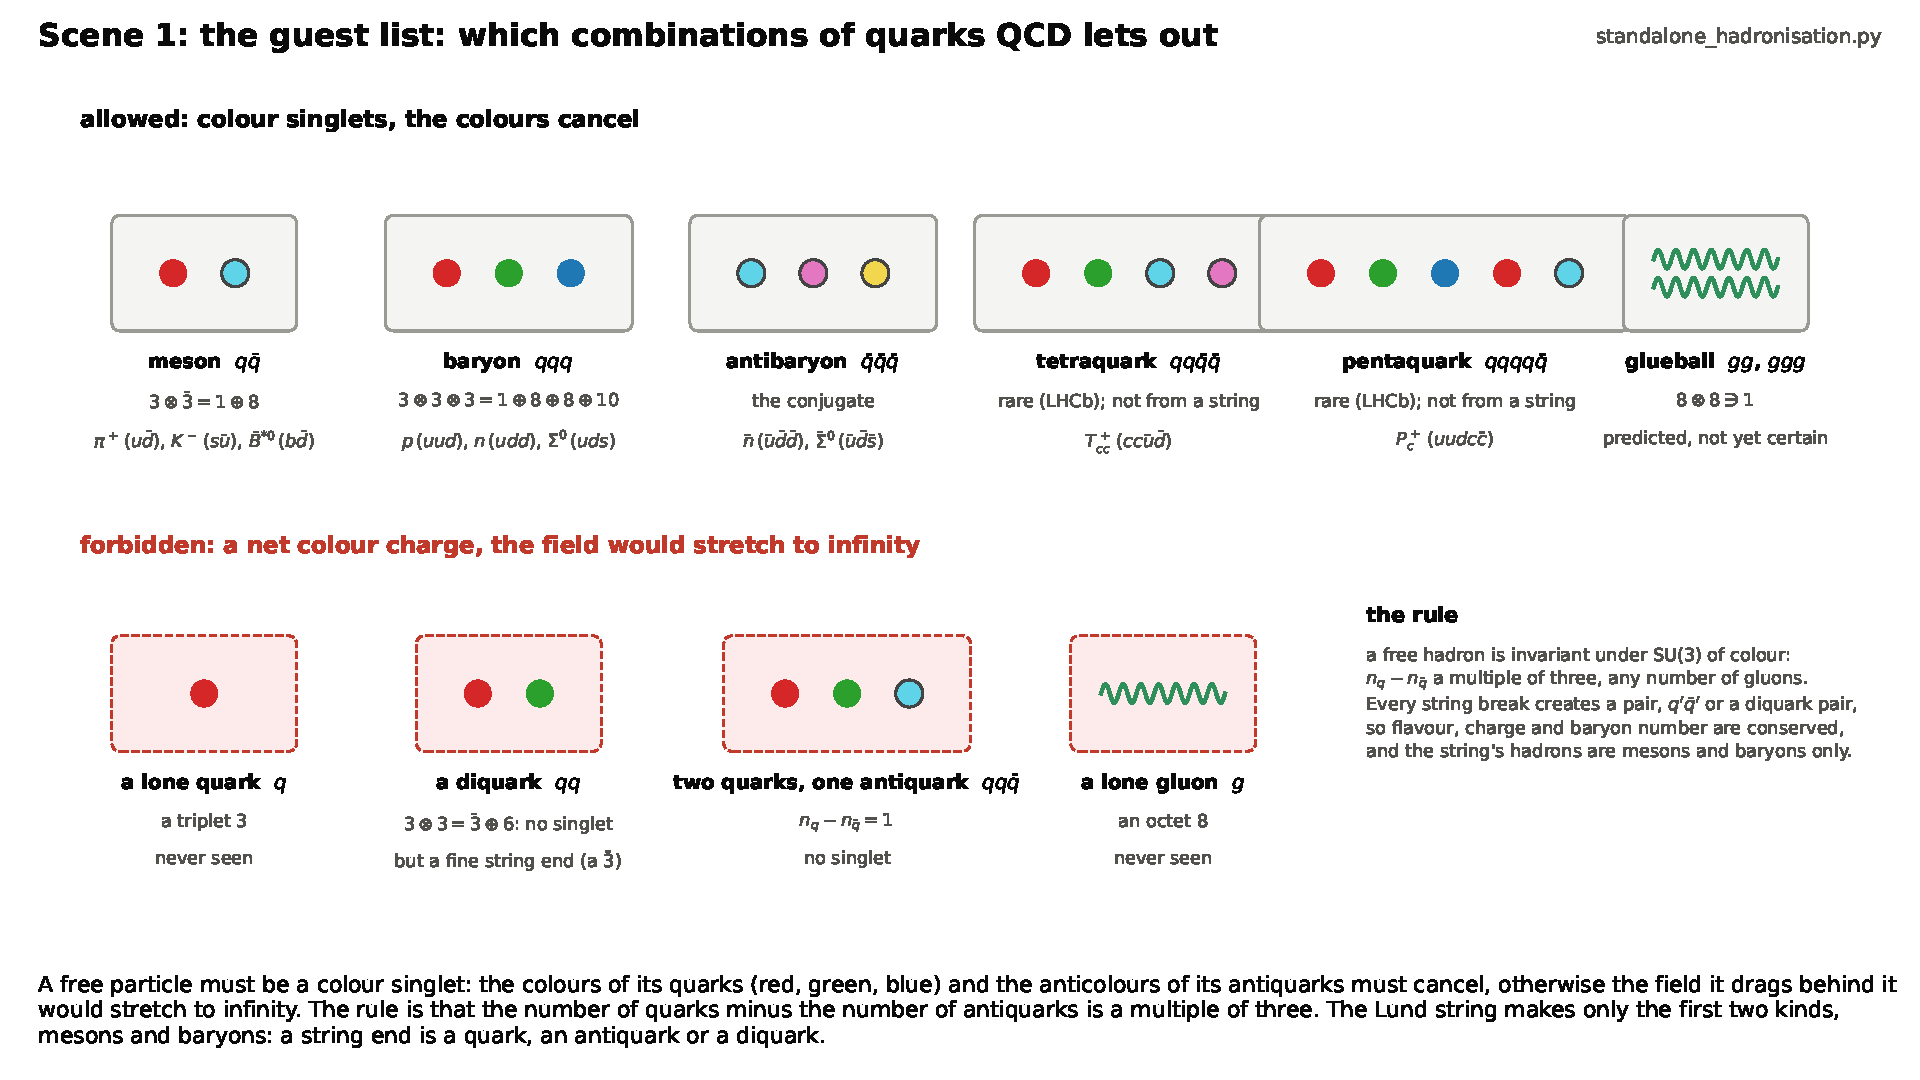
\includegraphics[page=1,width=0.325\textwidth]{Had/Standalone/animate_standalone_hadronisation_stills.pdf}\hfill
\includegraphics[page=2,width=0.325\textwidth]{Had/Standalone/animate_standalone_hadronisation_stills.pdf}\hfill
\includegraphics[page=3,width=0.325\textwidth]{Had/Standalone/animate_standalone_hadronisation_stills.pdf}\\[1.5mm]
\includegraphics[page=4,width=0.325\textwidth]{Had/Standalone/animate_standalone_hadronisation_stills.pdf}\hfill
\includegraphics[page=5,width=0.325\textwidth]{Had/Standalone/animate_standalone_hadronisation_stills.pdf}\hfill
\includegraphics[page=6,width=0.325\textwidth]{Had/Standalone/animate_standalone_hadronisation_stills.pdf}\\[1.5mm]
\includegraphics[page=7,width=0.325\textwidth]{Had/Standalone/animate_standalone_hadronisation_stills.pdf}\hfill
\includegraphics[page=8,width=0.325\textwidth]{Had/Standalone/animate_standalone_hadronisation_stills.pdf}\hfill
\includegraphics[page=9,width=0.325\textwidth]{Had/Standalone/animate_standalone_hadronisation_stills.pdf}
\caption[Key frames of the animated standalone hadronisation stage]{Key
frames of the nine scenes of the animated standalone hadronisation stage,
drawn by \file{animate_standalone_hadronisation.py} with \code{--stills},
in reading order. The guest list of colour singlets; the wedding, the
mother's rope snapping into its chain of sixteen hadrons; a generic rope
snapshot by snapshot with its world sheet in light-cone coordinates; the
mother's rope break by break down to the final two and the chain with its
vacuum pairs; a $28\GeV$ two-parton string breaking in its rest frame; the
$b$ quark's string producing its sixteen hadrons from both ends in the
$(\eta,\phi)$ plane; the two ends walking through the regions of the world
sheet; the whole event, 33 strings becoming 365 hadrons; and four hundred
hadronisations of the same partons against the \PYTHIA reference. The film itself
is the fifth on the playlist of \jitjetworld.}
\label{fig:children_getting_married:stills}
\end{figure}

\paragraph{The picture to carry: the wedding.}
Every stop so far had a
building: the contractors of \cref{ch:mother_gives_birth}, the other tenants
of \cref{ch:uninvited_cousins}. This stop empties it. Every parton in the
record holds one end of a rope, a colour line, and the rope's other end is
held by another parton, sometimes next door, sometimes across the whole
event. Nobody may leave the building alone. As the partons fly apart the
ropes stretch, and a stretched rope stores energy in proportion to its
length, one GeV per fermi; when a rope holds enough it snaps, and at the
break a new pair appears, each holding one of the new ends, so that there
are now two shorter ropes and still nobody is alone. This goes on until
every rope is too short to snap again, and what is left is a procession of
couples and triples, the hadrons, walking out in the directions their ropes
pointed (\cref{fig:children_getting_married:wedding_sketch}). The mother holds one end of a rope with four knots in it, the
gluons of \cref{ch:mother_gives_birth}, and she is heavy: she moves slowly
compared with the rope, the rope cannot pull much energy away from her, and
she leaves in a couple that carries nearly everything she had. The picture
captures the three things the chapter derives: a linear potential, pair
creation at the breaks, and a heavy end that keeps its momentum. Its limit
is that the rope is a classical object with quantum rules attached by hand,
and the rules have knobs: the Monash tune~\cite{Skands:2014pea}, which CP5
keeps unchanged for this stage.

\begin{figure}[htbp]\centering
\resizebox{\textwidth}{!}{% ---------------------------------------------------------------------------
% The wedding: the chain of mesons and baryons. (a) The mother's rope as the
% shower left it, b g g g g ubar, one colour line with four kinks, and one of
% the 32 other ropes of the record. (b) The rope snaps: at every break a
% quark-antiquark pair (or a diquark pair) appears from the vacuum, each new
% quark holding one of the new ends, so that nobody is ever alone. (c) The
% procession that leaves the house: the sixteen hadrons of the b quark's
% string in their order along the rope (the -v log, string 1), couples
% (mesons, q qbar) and triples (baryons, qqq); the original b sits in the
% first, the original ubar in the last, every other quark came out of the
% vacuum at a break.
% ---------------------------------------------------------------------------
\begin{tikzpicture}[x=1cm,y=1cm,
  every node/.style={font=\footnotesize},
  q/.style={circle,inner sep=0pt,minimum size=2.4mm,fill=red!80!black},
  aq/.style={circle,inner sep=0pt,minimum size=2.4mm,fill=blue!80!black},
  g/.style={circle,inner sep=0pt,minimum size=2.0mm,fill=green!50!black},
  nq/.style={circle,inner sep=0pt,minimum size=2.0mm,fill=green!50!black},
  naq/.style={circle,inner sep=0pt,minimum size=2.0mm,fill=green!50!black,draw=black,line width=0.5pt},
  rope/.style={orange!80!black,line width=2.2pt},
  had/.style={rounded corners=2pt,draw=black!60,fill=white,minimum width=9.6mm,minimum height=8mm,inner sep=1pt},
  lab/.style={font=\scriptsize,align=center},
  tiny/.style={font=\tiny,align=center},
  head/.style={font=\small\bfseries}]
% ---------------- (a) the ropes -----------------------------------------------------------------
\node[head,anchor=west] at (-9.0,3.55) {(a) the ropes: every parton holds one end of a colour line};
\node[q] (b) at (-8.4,2.4) {};
\node[g] (g1) at (-6.4,2.95) {}; \node[g] (g2) at (-4.6,2.15) {}; \node[g] (g3) at (-2.6,2.85) {}; \node[g] (g4) at (-0.8,2.25) {};
\node[aq] (ub) at (1.2,2.6) {};
\draw[rope] (b) -- (g1) -- (g2) -- (g3) -- (g4) -- (ub);
\node[lab,below=1pt of b] {$b$, the mother}; \node[lab,above=1pt of g1,text=green!40!black] {$g$}; \node[lab,below=1pt of g2,text=green!40!black] {$g$};
\node[lab,above=1pt of g3,text=green!40!black] {$g$}; \node[lab,below=1pt of g4,text=green!40!black] {$g$}; \node[lab,below=1pt of ub] {$\bar u$, from a cousin};
\node[lab,text=black!65] at (-3.6,1.35) {string~1 of the record: $W=69.3\GeV$, one rope with four knots};
\node[q] (u2) at (3.6,2.4) {}; \node[aq] (s2) at (6.2,2.4) {};
\draw[rope] (u2) -- (s2);
\node[lab,below=1pt of u2] {$u$}; \node[lab,below=1pt of s2] {$\bar s$};
\node[lab,text=black!65] at (4.9,3.05) {string~20: $27.5\GeV$};
\node[lab,text=black!65,anchor=west] at (6.9,2.4) {$\ldots$ and 31 more ropes: 33 colour singlets,\\ every colour tag held at both ends};
% ---------------- (b) the ropes snap ------------------------------------------------------------
\node[head,anchor=west] at (-9.0,0.45) {(b) the ropes snap: a pair from the vacuum at every break, nobody is left alone};
\node[q] (bb) at (-8.4,-0.5) {}; \node[aq] (ue) at (6.2,-0.5) {};
\node[lab,below=1pt of bb] {$b$}; \node[lab,below=1pt of ue] {$\bar u$};
\foreach \xl/\xr in {-8.3/-6.9, -5.9/-4.4, -3.4/-1.4, -0.4/1.6, 2.6/4.3, 5.3/6.1} {\draw[rope] (\xl,-0.5) -- (\xr,-0.5);}
\foreach \x/\p/\ap in {-6.4/{$d$}/{$\bar d$}, -3.9/{$d$}/{$\bar d$}, -0.9/{$u$}/{$\bar u$}, 2.1/{$d$}/{$\bar d$}, 4.8/{$u$}/{$\bar u$}} {
  \node[naq] at (\x-0.3,-0.5) {}; \node[nq] at (\x+0.3,-0.5) {};
  \node[tiny,text=green!40!black] at (\x-0.3,-0.15) {\ap}; \node[tiny,text=green!40!black] at (\x+0.3,-0.15) {\p};
  \draw[-{Stealth},green!40!black,thin] (\x-0.3,-0.75) -- (\x-0.6,-0.75); \draw[-{Stealth},green!40!black,thin] (\x+0.3,-0.75) -- (\x+0.6,-0.75);}
\node[lab,text=black!65,anchor=west] at (6.9,-0.5) {each break: $\kappa\,r$ of rope energy\\ paid for one $q'\bar q'$ (or diquark) pair;\\ the pieces that are left are the hadrons};
% ---------------- (c) the procession ------------------------------------------------------------
\node[head,anchor=west] at (-9.0,-1.75) {(c) the procession: the sixteen hadrons of the mother's rope, couples and triples, in their order along the rope};
\def\wedmeson#1#2#3#4#5{\node[had] (h#1) at (#1*1.1-8.25,-2.9) {};
  \node[#4] at (#1*1.1-8.25-0.18,-2.75) {}; \node[#5] at (#1*1.1-8.25+0.18,-2.75) {};
  \node[tiny] at (#1*1.1-8.25,-3.12) {#3}; \node[lab,anchor=south] at (#1*1.1-8.25,-2.48) {#2};}
\def\wedbaryon#1#2#3#4#5#6{\node[had] (h#1) at (#1*1.1-8.25,-2.9) {};
  \node[#4] at (#1*1.1-8.25-0.26,-2.75) {}; \node[#5] at (#1*1.1-8.25,-2.75) {}; \node[#6] at (#1*1.1-8.25+0.26,-2.75) {};
  \node[tiny] at (#1*1.1-8.25,-3.12) {#3}; \node[lab,anchor=south] at (#1*1.1-8.25,-2.48) {#2};}
\wedmeson{0}{$\bar B^{*0}$}{$b\bar d$}{q}{naq}
\wedmeson{1}{$\eta'$}{$d\bar d$}{nq}{naq}
\wedmeson{2}{$\rho^-$}{$d\bar u$}{nq}{naq}
\wedmeson{3}{$\pi^0$}{$u\bar u$}{nq}{naq}
\wedmeson{4}{$\rho^+$}{$u\bar d$}{nq}{naq}
\wedmeson{5}{$\pi^0$}{$d\bar d$}{nq}{naq}
\wedmeson{6}{$\pi^-$}{$d\bar u$}{nq}{naq}
\wedmeson{7}{$\rho^+$}{$u\bar d$}{nq}{naq}
\wedmeson{8}{$\pi^-$}{$d\bar u$}{nq}{naq}
\wedmeson{9}{$K^+$}{$u\bar s$}{nq}{naq}
\wedmeson{10}{$\bar K^{*0}$}{$s\bar d$}{nq}{naq}
\wedmeson{11}{$\pi^0$}{$d\bar d$}{nq}{naq}
\wedmeson{12}{$\pi^-$}{$d\bar u$}{nq}{naq}
\wedbaryon{13}{$\Sigma^0$}{$uds$}{nq}{nq}{nq}
\wedbaryon{14}{$\bar\Sigma^0$}{$\bar u\bar d\bar s$}{naq}{naq}{naq}
\wedmeson{15}{$\pi^0$}{$u\bar u$}{nq}{aq}
\draw[decorate,decoration={brace,mirror,amplitude=3pt}] (-8.7,-3.45) -- (-7.8,-3.45) node[midway,below=3pt,lab] {the\\ mother's $b$};
\draw[decorate,decoration={brace,mirror,amplitude=3pt}] (7.8,-3.45) -- (8.7,-3.45) node[midway,below=3pt,lab] {the\\ original $\bar u$};
\draw[decorate,decoration={brace,mirror,amplitude=3pt}] (-7.6,-3.45) -- (7.6,-3.45) node[midway,below=3pt,lab,text width=11cm] {the fourteen quarks and antiquarks in between came out of the vacuum at the breaks; a diquark pair gives a baryon and an antibaryon side by side};
\end{tikzpicture}
}
\caption[The wedding: the ropes of the record and the chain of mesons and
baryons]{The wedding. Top: the mother's rope, $b\,g\,g\,g\,g\,\bar u$, one
colour line with four knots, and one of the 32 other ropes of the record.
Middle: the rope snaps, and at every break a pair from the vacuum takes the
two new ends. Bottom: the procession that leaves the house, the sixteen
hadrons of the mother's rope in their order along it from the \code{-v}
log, couples (mesons, $q\bar q$) and triples (baryons, $qqq$) with their
quark content; the mother's $b$ is in the first, the original $\bar u$ in
the last, and every other quark came out of the vacuum at a break.}
\label{fig:children_getting_married:wedding_sketch}
\end{figure}

\paragraph{The number, three ways.}
\label{sec:children_getting_married:validation}
\label{sec:children_getting_married:standalone_code}
\Cref{tab:children_getting_married:numbers} gives away the ending. Its
sharpest column pair is new: for the first time the standalone script and
\PYTHIA can be run on \emph{identical} input, the 211 partons of
\file{event_MPI.lhe} with their colour tags, so that the comparison is
between two implementations of the same model and nothing else. The two
agree on the hadron multiplicity to $5\%$, on the B~hadron's energy fraction
to $0.03$, and on what the detector will see, the hadron-level cone around
the $b$, to $1.2\GeV$ at $R=0.4$. The other columns are \PYTHIA's full chain
from the hard event, with the impact parameter drawn and fixed as in
\cref{ch:uninvited_cousins}, and the single \CMSSW event.

The standalone script is a port of \PYTHIA~8's six string classes, from
\code{ColourTracing} to \code{MiniStringFragmentation}, into Python that
needs NumPy and nothing else; it imports the shower script of
\cref{ch:mother_gives_birth} for the record and the Lorentz frames, and its
hadron table was read once from \PYTHIA's own particle data. Its learning
mode, \code{-v}, prints the parameters of the model, the table of all $33$
colour singlets, and then, for the string that holds the $b$ quark, every
hadron in production order with the end it came from, the flavour draw and
its weights, the \pt kick, the fragmentation function and the $z$ drawn,
the proper time of the vertex and the regions stepped through, down to the
final two; \code{-vv} does the same for every string. The $2200$ lines of
\code{-v} for seed~1 are committed, and every number quoted in the theory
of this chapter is taken from that log.
\label{sec:children_getting_married:pythia}

The first official check is the sharpest in the book so far: \PYTHIA with
its process level switched off, its record filled by hand with the $211$
partons of \file{event_MPI.lhe} and their colour tags, hadronising them
four hundred times with the Monash fragmentation parameters that CP5
keeps and decays off, against the standalone script doing the same. Read
the first two columns of the table together. \PYTHIA finds the same $33$
colour singlets and joins the same $48$ partons. It makes $383$ hadrons
where the script makes $402$, and the $5\%$ excess has an address: the
gluon-rich strings, $46$ against $43$ hadrons from the $108\GeV$ string
with $21$ partons, while the two-parton strings agree to $2\%$; the region
bookkeeping of \cref{sec:children_getting_married:kinks} is where the two
implementations differ in detail. The script makes $11\%$ fewer baryons
because it has no popcorn mechanism, \PYTHIA's option of putting a meson
between a baryon and its antibaryon. The B~hadron keeps $0.03$ less of the
quark's energy, for every choice of fragmentation function. What the
detector will see agrees better than any of these: the hadron-level \pt
within $\dR<0.4$ of the $b$ differs by $1.2\GeV$ between the two and within
$\dR<0.8$ by $0.4\GeV$, the cone masses agree to $0.5\GeV$, and the species
to a percent. The full chain with $b$ drawn gives $226\pm87$ hadrons, a
wide distribution because the number of secondary scatterings is wide; at
the \CMSSW impact parameter it gives $306\pm52$, and the \CMSSW event's
$320$ sits inside.
\label{sec:children_getting_married:cmssw}

The second official check is the \code{GEN} step of
\cref{sec:ancestral_home:cmssw} with the hadronisation switched on and the
decays still off; in production \code{HadronLevel:all} is on in every CMS
configuration, with the Monash values that \code{Tune:pp = 14} selects and
that the script embeds. Its
event is the last column of the table, and
\cref{sec:children_getting_married:our_jet_at_this_stage_the_hadron_level_f}
follows the mother through its record. How each column was produced, the
commands, the modes and the logs, is in the companion of this chapter,
\begin{center}
  \companion{chapter_05_Had}
\end{center}
together with the full tables behind every number quoted below.

\begin{table}[htbp]\centering\small
\caption[Hadronisation obtained three ways]{Hadronisation obtained three
ways. ``Same partons'' means the 211 final partons of
\file{example/MPI/event_MPI.lhe} with their colour tags, hadronised $400$
times by \PYTHIA~8.315 with the Monash fragmentation parameters that CP5
keeps, and $400$ times by the standalone script; ``full chain'' means
\PYTHIA from the hard event of \cref{ch:ancestral_home} with the CP5
settings, $2000$ events with $b$ drawn and $526$ with
$|b/\langle b\rangle-0.3136|<0.03$; hadron decays are off everywhere, so
every hadron is primary. The spread of a single event follows $\pm$. Cones
are drawn around the final copy of the $b$ quark; the $B$ share is the
hadron's \pt over the cone's. The species row lists $\bar B^{*0}$ and
$\bar B^0$ ($b\bar d$), $B^{*-}$ and $B^-$ ($b\bar u$) and $\bar B_s^{*0}$
($b\bar s$). The \CMSSW column is the single event of
\cref{ch:ancestral_home}, read from its log.}
\label{tab:children_getting_married:numbers}
\scriptsize\setlength{\tabcolsep}{3pt}
\resizebox{\textwidth}{!}{%
\begin{tabular}{lrrrrrr}\toprule
 & \PYTHIA & standalone & \PYTHIA full & \PYTHIA full & standalone & \CMSSW \\
 & same partons & same partons & $b$ drawn & $b=0.3136$ & seed 1 & 1 event \\ \midrule
primary hadrons & $383\pm11$ & $402\pm14$ & $226\pm87$ & $306\pm52$ & $365$ & $320$ \\
\quad charged & $207.5\pm11.9$ & $217.2\pm12.5$ & $122\pm48$ & $165\pm29$ & $184$ & $169$ \\
\quad baryons & $44.0\pm7.6$ & $38.8\pm7.6$ & $26.8$ & $36.3$ & $52$ & $34$ \\
\quad with strangeness & $87.8\pm10.3$ & $92.1\pm10.5$ & $49.6$ & $67.8$ & $94$ & $66$ \\
\quad at $|\eta|<2.5$ & $193.8$ & $206.3$ & $91.9$ & $128.3$ & $179$ & $141$ \\
colour singlets, partons joined & $33$, $48$ & $33$, $48$ & -- & -- & $33$, $48$ & $26$, $45$ \\ \midrule
$b$: $\xE=E_B/E_b$ (Lund--Bowler) & $0.913\pm0.062$ & $0.882\pm0.078$ & $0.941\pm0.100$ & $0.931\pm0.089$ & $1.004$ & $1.025$ \\
$b$: \xE, plain Lund ($r_b=0$) & $0.963\pm0.038$ & $0.952\pm0.048$ & -- & -- & -- & -- \\
$b$: \xE, Peterson ($\epsilon_b=0.005$) & $0.870\pm0.120$ & $0.839\pm0.132$ & -- & -- & -- & -- \\
$\bar b$: \xE & $1.033\pm0.049$ & $1.025\pm0.072$ & $0.941\pm0.095$ & $0.936\pm0.094$ & $1.154$ & $0.980$ \\
$b$: \pt of its hadron [GeV] & $71.1\pm5.0$ & $69.4\pm5.2$ & $87.8\pm26.7$ & $87.7\pm27.3$ & $78.56$ & $94.28$ \\
$b$: $\bar B^{*0}\!:\!B^{*-}\!:\!\bar B^0\!:\!B^-\!:\!\bar B_s^{*0}$ [\%] & $31:28:14:12:8$ & $31:32:13:12:6$ & $29:29:13:15:6$ & $30:29:14:14:4$ & \Bstarbar & $B^-$ \\ \midrule
$b$, $\dR<0.4$: partons \pt [GeV] & $100.67$ & $100.67$ & $109.7$ & $109.7$ & $100.67$ & $127.25$ \\
$b$, $\dR<0.4$: hadrons \pt [GeV] & $98.0\pm2.2$ & $96.8\pm3.1$ & $109.6$ & $109.8$ & $99.23$ & $114.45$ \\
$b$, $\dR<0.4$: hadrons, mass [GeV] & $7.6$, $17.2$ & $8.0$, $16.8$ & $6.2$, $14.3$ & $6.7$, $15.4$ & $6$, $16.1$ & $9$, $20.4$ \\
$b$, $\dR<0.4$: $B$ share of the cone \pt & $0.726$ & $0.710$ & $0.800$ & $0.799$ & $0.79$ & $0.82$ \\
$b$, $\dR<0.8$: partons \pt [GeV] & $104.09$ & $104.09$ & $118.4$ & $120.0$ & $104.09$ & -- \\
$b$, $\dR<0.8$: hadrons \pt [GeV] & $104.2\pm1.8$ & $104.6\pm2.5$ & $118.7$ & $120.6$ & $105.98$ & $141.1$ \\
$b$, $\dR<0.8$: hadrons, mass [GeV] & $15.1$, $31.6$ & $16.6$, $32.5$ & $12.0$, $28.1$ & $14.2$, $32.9$ & $14$, $35.9$ & $28$, $49.8$ \\
\bottomrule
\end{tabular}}
\end{table}

\section{Let us dive into the details: the theory}
\label{sec:children_getting_married:theory}

\subsection{From partons to hadrons: the Lund string}
\label{sec:children_getting_married:from_partons_to_hadrons_the_lund_string}

Before the rope, the guest list: who is allowed to leave the house at all.
QCD lets only colour singlets out, states in which the colour charges
cancel, because anything that carries a net colour charge drags a flux
tube behind it whose energy grows without bound
(\cref{fig:children_getting_married:singlets_sketch}). A quark and an
antiquark can cancel, $\mathbf3\otimes\bar{\mathbf3}$ contains a singlet,
and that is a \emph{meson}; three quarks can, $\mathbf3\otimes\mathbf3\otimes\mathbf3$
contains a singlet, and that is a \emph{baryon}, with the antibaryon its
conjugate. Two quarks cannot, $\mathbf3\otimes\mathbf3=\bar{\mathbf3}\oplus\mathbf6$
has no singlet, so a diquark is never free, although it behaves as an
antiquark, a $\bar{\mathbf3}$, at the end of a string and that is how
baryons will be made; two quarks and an antiquark cannot either, and
neither can a single gluon. The general rule is that the number of quarks
minus the number of antiquarks must be a multiple of three, with any
number of gluons added, which also allows tetraquarks $qq\bar q\bar q$,
pentaquarks $qqqq\bar q$ and glueballs: the first two exist and are rare,
LHCb has seen a $T_{cc}^+$ ($cc\bar u\bar d$) and the $P_c$ states
($uudc\bar c$), the third is predicted and not yet identified for certain.
The Lund string produces none of them. Its ends are quarks, antiquarks and
diquarks, so every break makes a meson or a baryon--antibaryon pair of
neighbours, and the 365 hadrons of our event are all of the first two
kinds: 313 mesons and 52 baryons. With the guest list settled, the rest of
the section is about the rope.

\begin{figure}[htbp]\centering
\resizebox{\textwidth}{!}{% ---------------------------------------------------------------------------
% What QCD lets out of the house. A free particle must be a colour singlet:
% the allowed combinations are those in which the colours cancel, a quark
% with an antiquark (3 x 3bar contains 1), three quarks or three antiquarks
% (3 x 3 x 3 contains 1), and the rarer multiquark states and glueballs; a
% lone quark, a diquark (3 x 3 = 3bar + 6, no singlet) or a q q qbar carry
% colour and are forbidden. The Lund string makes only the first row's
% mesons and baryons: its ends are quarks, antiquarks and diquarks.
% ---------------------------------------------------------------------------
\begin{tikzpicture}[x=1cm,y=1cm,
  every node/.style={font=\footnotesize},
  cr/.style={circle,inner sep=0pt,minimum size=2.8mm,fill=red!85!black},
  cg/.style={circle,inner sep=0pt,minimum size=2.8mm,fill=green!60!black},
  cb/.style={circle,inner sep=0pt,minimum size=2.8mm,fill=blue!75!black},
  ar/.style={circle,inner sep=0pt,minimum size=2.8mm,fill=cyan!70,draw=black!60,line width=0.4pt},
  ag/.style={circle,inner sep=0pt,minimum size=2.8mm,fill=magenta!60,draw=black!60,line width=0.4pt},
  ab/.style={circle,inner sep=0pt,minimum size=2.8mm,fill=yellow!85!orange,draw=black!60,line width=0.4pt},
  bag/.style={rounded corners=5pt,draw=black!55,fill=black!4,minimum height=11mm,inner sep=2pt},
  bad/.style={rounded corners=5pt,draw=red!70!black,dashed,fill=red!5,minimum height=11mm,inner sep=2pt},
  lab/.style={font=\scriptsize,align=center,text width=2.8cm},
  rule/.style={font=\scriptsize,align=left},
  head/.style={font=\small\bfseries}]
% ---------------- allowed --------------------------------------------------------------------------
\node[head,anchor=west] at (-0.5,3.55) {allowed: colour singlets, the colours cancel};
% meson at x = 0.9
\node[bag,minimum width=14mm] at (0.9,2.6) {}; \node[cr] at (0.6,2.6) {}; \node[ar] at (1.2,2.6) {};
\node[lab,anchor=north] at (0.9,1.95) {\textbf{meson} $q\bar q$\\ $\mathbf3\otimes\bar{\mathbf3}=\mathbf1\oplus\mathbf8$\\ $\pi^+\,(u\bar d)$, $K^-\,(s\bar u)$,\\ $\bar B^{*0}\,(b\bar d)$};
% baryon at x = 3.9
\node[bag,minimum width=18mm] at (3.9,2.6) {}; \node[cr] at (3.4,2.6) {}; \node[cg] at (3.9,2.6) {}; \node[cb] at (4.4,2.6) {};
\node[lab,anchor=north] at (3.9,1.95) {\textbf{baryon} $qqq$\\ $\mathbf3\otimes\mathbf3\otimes\mathbf3=\mathbf1\oplus\mathbf8\oplus\mathbf8\oplus\mathbf{10}$\\ $p\,(uud)$, $n\,(udd)$,\\ $\Sigma^0\,(uds)$};
% antibaryon at x = 6.9
\node[bag,minimum width=18mm] at (6.9,2.6) {}; \node[ar] at (6.4,2.6) {}; \node[ag] at (6.9,2.6) {}; \node[ab] at (7.4,2.6) {};
\node[lab,anchor=north] at (6.9,1.95) {\textbf{antibaryon} $\bar q\bar q\bar q$\\ the conjugate\\ $\bar n\,(\bar u\bar d\bar d)$,\\ $\bar\Sigma^0\,(\bar u\bar d\bar s)$};
% tetraquark at x = 10.0
\node[bag,minimum width=22mm] at (10.0,2.6) {}; \node[cr] at (9.3,2.6) {}; \node[cg] at (9.75,2.6) {}; \node[ar] at (10.25,2.6) {}; \node[ag] at (10.7,2.6) {};
\node[lab,anchor=north] at (10.0,1.95) {\textbf{tetraquark} $qq\bar q\bar q$\\ rare, seen by LHCb\\ $T_{cc}^+\,(cc\bar u\bar d)$,\\ not from a string};
% pentaquark at x = 13.2
\node[bag,minimum width=26mm] at (13.2,2.6) {}; \node[cr] at (12.3,2.6) {}; \node[cg] at (12.75,2.6) {}; \node[cb] at (13.2,2.6) {}; \node[cr] at (13.65,2.6) {}; \node[ar] at (14.1,2.6) {};
\node[lab,anchor=north] at (13.2,1.95) {\textbf{pentaquark} $qqqq\bar q$\\ rare, seen by LHCb\\ $P_c^+\,(uudc\bar c)$,\\ not from a string};
% glueball at x = 16.2
\node[bag,minimum width=16mm] at (16.2,2.6) {};
\draw[decorate,decoration={coil,aspect=0.6,segment length=1.4mm,amplitude=1mm},green!50!black,thick] (15.6,2.45) -- (16.8,2.45);
\draw[decorate,decoration={coil,aspect=0.6,segment length=1.4mm,amplitude=1mm},green!50!black,thick] (15.6,2.75) -- (16.8,2.75);
\node[lab,anchor=north] at (16.2,1.95) {\textbf{glueball} $gg$, $ggg$\\ predicted, not yet\\ identified for certain\\ ($\mathbf8\otimes\mathbf8\ni\mathbf1$)};
% ---------------- forbidden ------------------------------------------------------------------------
\node[head,anchor=west] at (-0.5,-0.35) {forbidden: a net colour charge, the field would stretch to infinity};
\node[bad,minimum width=10mm] at (0.9,-1.3) {}; \node[cr] at (0.9,-1.3) {};
\node[lab,anchor=north] at (0.9,-1.95) {\textbf{a lone quark} $q$\\ a triplet $\mathbf3$:\\ never seen};
\node[bad,minimum width=14mm] at (3.9,-1.3) {}; \node[cr] at (3.6,-1.3) {}; \node[cg] at (4.2,-1.3) {};
\node[lab,anchor=north] at (3.9,-1.95) {\textbf{a diquark} $qq$\\ $\mathbf3\otimes\mathbf3=\bar{\mathbf3}\oplus\mathbf6$:\\ no singlet, but a fine\\ string end (it is a $\bar{\mathbf3}$)};
\node[bad,minimum width=18mm] at (6.9,-1.3) {}; \node[cr] at (6.4,-1.3) {}; \node[cg] at (6.9,-1.3) {}; \node[ar] at (7.4,-1.3) {};
\node[lab,anchor=north] at (6.9,-1.95) {\textbf{two quarks and}\\ \textbf{an antiquark} $qq\bar q$\\ $n_q-n_{\bar q}=1$:\\ no singlet};
\node[bad,minimum width=14mm] at (10.0,-1.3) {};
\draw[decorate,decoration={coil,aspect=0.6,segment length=1.4mm,amplitude=1mm},green!50!black,thick] (9.45,-1.3) -- (10.55,-1.3);
\node[lab,anchor=north] at (10.0,-1.95) {\textbf{a lone gluon} $g$\\ an octet $\mathbf8$:\\ never seen};
\node[rule,anchor=north west,text width=5.6cm] at (11.7,-0.65) {\textbf{the rule}: a free hadron is invariant under $\mathrm{SU}(3)_{\mathrm c}$, which needs $n_q-n_{\bar q}$ to be a multiple of three, with any number of gluons; the quark model's mesons and baryons are the two cheapest ways, and they are the only two the Lund string produces, because a string end is a quark, an antiquark or a diquark. The baryon number $(n_q-n_{\bar q})/3$ and the flavours are conserved in every break: the vacuum pair is always $q'\bar q'$ or $(q'q'')(\overline{q'q''})$.};
\end{tikzpicture}
}
\caption[Which combinations of quarks and antiquarks QCD lets out]{Which
combinations of quarks, antiquarks and gluons QCD lets out of the house.
Top: the colour singlets, with the colour of each quark drawn and the
anticolour of each antiquark drawn in the complementary shade: mesons and
baryons, which the Lund string produces, and the rarer tetraquarks,
pentaquarks and glueballs, which it does not. Bottom: combinations with a
net colour charge, which are never free; the diquark among them is a fine
string end. Every hadron that is named carries its quark content in
brackets, the convention of this chapter.}
\label{fig:children_getting_married:singlets_sketch}
\end{figure}

\subsubsection{A rope between the dancers: the linear potential and the area law}
\label{sec:children_getting_married:string}

Guess first. Two partons of our record fly apart, a $u$ quark and an $\bar s$
antiquark from one of the secondary scatterings, with $27.5\GeV$ of
invariant mass between them. In QED they would simply separate, the field
between them falling as $1/r^2$. What happens in QCD? The gluons carry
colour themselves and attract one another, and the field between a colour
charge and an anticolour charge does not spread out but collapses into a
tube of constant cross section, so that its energy grows in proportion to
its length. The lattice confirms the picture and measures the constant: the
potential between a static quark and antiquark is
\begin{equation}
  V(r)=\kappa r,\qquad \kappa\approx1\GeV/\mathrm{fm}=0.197\GeV^2,
  \label{eq:children_getting_married:potential}
\end{equation}
the \emph{string tension}, at distances beyond half a fermi. Our two
partons would stretch a $28\,\mathrm{fm}$ string before the tension stopped
them, and $28\,\mathrm{fm}$ of string holds $28\GeV$: far more than the
mass of a few quark pairs. The string does not get that long. It breaks,
and this subsection is about where.

\begin{figure}[htbp]\centering
\resizebox{\textwidth}{!}{% ---------------------------------------------------------------------------
% The Lund string. (a) The colour field between a quark and an antiquark is
% a tube of constant energy per length, kappa = 1 GeV/fm, so V(r) = kappa r.
% (b) The world sheet of a two-parton string in its rest frame: the two ends
% fly apart at the speed of light, the string between them breaks at
% vertices that lie near a hyperbola of constant proper time, and every
% piece between two neighbouring vertices is one hadron. (c) The numbers of
% our event (the -v log, "the colour-singlet strings of the record").
% ---------------------------------------------------------------------------
\begin{tikzpicture}[x=1cm,y=1cm,
  every node/.style={font=\footnotesize},
  q/.style={circle,inner sep=0pt,minimum size=2.4mm,fill=red!80!black},
  aq/.style={circle,inner sep=0pt,minimum size=2.4mm,fill=blue!80!black},
  vtx/.style={circle,inner sep=0pt,minimum size=1.8mm,fill=black},
  lab/.style={font=\scriptsize,align=center},
  head/.style={font=\small\bfseries}]
% ---------------- (a) the flux tube ----------------------------------------------------------
\begin{scope}
\node[head,anchor=west] at (-0.3,3.3) {(a) the rope: $V(r)=\kappa r$};
\fill[orange!35] (0.6,1.75) rectangle (4.4,2.25);
\foreach \x in {0.8,1.2,...,4.2} {\draw[orange!70!black,thin] (\x,1.75) -- (\x+0.2,2.25);}
\node[q] (q) at (0.5,2.0) {}; \node[aq] (aq) at (4.5,2.0) {};
\node[lab,above=1pt of q] {$q$}; \node[lab,above=1pt of aq] {$\bar q$};
\draw[-{Stealth}] (q) -- ++(-0.6,0); \draw[-{Stealth}] (aq) -- ++(0.6,0);
\draw[{Stealth}-{Stealth},thin] (0.6,1.4) -- (4.4,1.4) node[midway,below,lab] {$r$};
\node[lab,anchor=north,text width=5.4cm] at (2.5,0.95) {energy stored: $\kappa r$ with $\kappa=1\GeV/\mathrm{fm}=0.197\GeV^2$; a $1\,\mathrm{fm}$ string holds $1\GeV$, enough for a $u\bar u$ pair.\\[2pt] \textcolor{black!65}{our $28\GeV$ two-parton string would stretch to $14+14\,\mathrm{fm}$ before turning round; it breaks long before}};
\end{scope}
% ---------------- (b) the world sheet --------------------------------------------------------
\begin{scope}[xshift=9.2cm,yshift=-0.3cm]
\node[head,anchor=west] at (-2.9,3.6) {(b) the world sheet breaks};
\begin{scope}[x=0.32cm,y=0.32cm]
\fill[orange!18] (0,0) -- (-8,8) -- (8,8) -- cycle;
\draw[-{Stealth}] (-8.5,0) -- (8.8,0) node[below left,lab] {$x$ [fm]};
\draw[-{Stealth}] (0,0) -- (0,9.2) node[left,lab] {$t$ [fm]};
\draw[red!80!black,thick] (0,0) -- (-8,8); \draw[blue!80!black,thick] (0,0) -- (8,8);
\node[lab,text=red!80!black] at (-7.3,8.7) {$q$}; \node[lab,text=blue!80!black] at (7.3,8.7) {$\bar q$};
% hyperbola of constant proper time tau = 1.5 fm: t = sqrt(x^2 + 2.25)
\draw[black!60,dashed] plot[domain=-7.5:7.5,samples=61] (\x,{sqrt(\x*\x+2.25)});
\node[lab,text=black!65,anchor=west] at (5.0,2.0) {$\Gamma=\kappa^2\tau^2=x^+x^-$};
% vertices at rapidities -2.0 -1.0 -0.2 0.6 1.4 2.2
\foreach \px/\pt in {-5.44/5.64,-1.76/2.31,-0.30/1.53,0.96/1.78,2.86/3.22,6.72/6.88} {
  \node[vtx] at (\px,\pt) {};
  \draw[black!70] (\px,\pt) -- ++(1.1,1.1); \draw[black!70] (\px,\pt) -- ++(-1.1,1.1);}
\node[lab,anchor=south] at (-3.6,6.2) {hadron};
\node[lab,anchor=south] at (-1.0,3.2) {hadron};
\node[lab,anchor=south] at (0.3,2.9) {$\cdots$};
\node[lab,anchor=south] at (4.8,7.4) {hadron};
\node[lab,anchor=north west,text width=5.6cm,text=black!65] at (-8.6,-1.3) {each break: a $q'\bar q'$ pair from the vacuum; the piece between two neighbouring vertices is one hadron, the end pieces carry the original $q$ and $\bar q$};
\end{scope}
\end{scope}
% ---------------- (c) the numbers --------------------------------------------------------------
\begin{scope}[xshift=12.9cm]
\node[head,anchor=west] at (-0.3,3.3) {(c) our event};
\node[lab,anchor=north west,text width=5.2cm,align=left] at (-0.3,3.0) {
211 partons, every colour tag once as colour and once as anticolour\\[2pt]
$\to$ 33 colour singlets: 29 strings and 4 ministrings, no closed gluon loop; 48 partons joined to a neighbour (pair mass within $0.3\GeV$ of the endpoint masses)\\[2pt]
total string mass $3071\GeV$; the heaviest, $1036\GeV$, runs from a remnant $d$ to a remnant $\bar u$; the $b$ quark's, $69.3\GeV$, has four gluons\\[2pt]
$\to$ 365 primary hadrons; a two-parton string gives $n\approx0.1+2.55\ln(W/\GeV)$: 7 from $28\GeV$, 18 from $1036\GeV$};
\end{scope}
\end{tikzpicture}
}
\caption[The Lund string, its world sheet and the strings of our event]{Left:
the colour field between a quark and an antiquark is a tube of constant
energy per length, so the potential is linear,
\cref{eq:children_getting_married:potential}. Middle: the world sheet of a
two-parton string in its rest frame: the ends move on the light cone, the
string breaks at vertices that sit near a hyperbola of constant proper
time, and every piece between two neighbouring vertices is one hadron.
Right: the strings of our event from the \code{-v} log.}
\label{fig:children_getting_married:string_sketch}
\end{figure}

Think of the string in its own rest frame, and watch it snapshot by
snapshot (\cref{fig:children_getting_married:lightcone_sketch}, bottom):
the quark and the antiquark are created at one point and fly apart at the
speed of light, the rope between them fills with energy, a pair appears
at rest somewhere along it and is pulled apart by the two pieces, more
pairs appear, and what is left are short pieces that no longer know about
one another, each a quark and an antiquark running towards each other,
crossing and running apart again for ever: a ``yo-yo'', the string
model's hadron. The natural coordinates for this are not $t$ and $x$ but
the two light-like combinations
\begin{equation}
  x^\pm=t\pm x,\qquad x^+x^-=t^2-x^2=\tau^2,
  \label{eq:children_getting_married:lightcone}
\end{equation}
the \emph{light-cone coordinates} of
\cref{fig:children_getting_married:lightcone_sketch}, top left: the two
light-cone lines through the origin become the axes, a massless quark at
the $+$ end starts at the origin and moves on $x^-=0$, the antiquark on
$x^+=0$, and the product of the two coordinates of any point is the square
of its proper time. The same combinations of a momentum, $p^\pm=E\pm p_x$,
obey $p^+p^-=\mT^2$, and the string tension turns the one into the other:
a piece of string of light-cone length $\Delta x^\pm$ carries
$p^\pm=\kappa\,\Delta x^\pm$. A break-up at the point $(x^+,x^-)$ is a
vertex on the world sheet, and two neighbouring vertices fix one hadron
(\cref{fig:children_getting_married:lightcone_sketch}, top right): the quark
born at the vertex nearer the $q$ end and the antiquark born at the vertex
nearer the $\bar q$ end run towards each other, and the diamond they sweep
is the hadron's yo-yo.

\begin{figure}[htbp]\centering
\resizebox{\textwidth}{!}{% ---------------------------------------------------------------------------
% How the world sheet breaks. (a) Light-cone coordinates in the string's rest
% frame: x+- = t +- x, so the two light-like directions are the axes, a
% massless quark end runs along one of them, and a point has x+ x- =
% t^2 - x^2 = tau^2, the hyperbola of constant proper time. (b) The same on
% the world sheet: the break-up vertices, and the diamond between two
% neighbouring vertices and their forward light-cones is one hadron, with
% m_T^2 = kappa^2 Dx+ Dx-. (c) Snapshots of the rope in time: the ends fly
% apart, the rope fills, a pair appears at a break, the pieces between
% neighbouring breaks are the hadrons, each a "yo-yo" that oscillates for
% ever.
% ---------------------------------------------------------------------------
\begin{tikzpicture}[x=1cm,y=1cm,
  every node/.style={font=\footnotesize},
  q/.style={circle,inner sep=0pt,minimum size=2.2mm,fill=red!80!black},
  aq/.style={circle,inner sep=0pt,minimum size=2.2mm,fill=blue!80!black},
  nq/.style={circle,inner sep=0pt,minimum size=1.9mm,fill=green!50!black},
  naq/.style={circle,inner sep=0pt,minimum size=1.9mm,fill=green!50!black,draw=black,line width=0.5pt},
  vtx/.style={circle,inner sep=0pt,minimum size=1.8mm,fill=black},
  rope/.style={orange!80!black,line width=2.0pt},
  lab/.style={font=\scriptsize,align=center},
  tiny/.style={font=\tiny,align=center},
  head/.style={font=\small\bfseries}]
% ---------------- (a) light-cone coordinates ----------------------------------------------------
\begin{scope}
\node[head,anchor=west] at (-3.4,4.55) {(a) light-cone coordinates $x^\pm=t\pm x$};
\fill[orange!15] (0,0) -- (-3.2,3.2) -- (3.2,3.2) -- cycle;
\draw[-{Stealth}] (-3.4,0) -- (3.6,0) node[below left,lab] {$x$};
\draw[-{Stealth}] (0,0) -- (0,3.9) node[left,lab] {$t$};
\draw[red!80!black,thick] (0,0) -- (3.3,3.3) node[above,lab,text=red!80!black] {$x^-=0$: the $q$ end\\ (the $x^+$ axis)};
\draw[blue!80!black,thick] (0,0) -- (-3.3,3.3) node[above,lab,text=blue!80!black] {$x^+=0$: the $\bar q$ end\\ (the $x^-$ axis)};
% point P at (x,t) = (0.8, 2.3): x+ = 3.1, x- = 1.5; feet at (x+/2)(1,1) = (1.55,1.55) and (x-/2)(-1,1) = (-0.75,0.75)
\node[vtx] (P) at (0.8,2.3) {}; \node[lab,anchor=south west] at (0.85,2.35) {a break at $(x,t)$};
\draw[dashed,black!60] (0.8,2.3) -- (1.55,1.55); \draw[dashed,black!60] (0.8,2.3) -- (-0.75,0.75);
\draw[decorate,decoration={brace,amplitude=3pt},red!80!black] (0,0) -- (1.55,1.55) node[midway,above left=1pt,lab,text=red!80!black] {$x^+/\sqrt2$};
\draw[decorate,decoration={brace,amplitude=3pt,mirror},blue!80!black] (0,0) -- (-0.75,0.75) node[midway,above right=1pt,lab,text=blue!80!black] {$x^-/\sqrt2$};
\draw[black!60,dashed,thin] plot[domain=-2.9:2.9,samples=41] (\x,{sqrt(\x*\x+2.25)});
\node[lab,text=black!65,anchor=west] at (2.0,1.7) {$x^+x^-=\tau^2$};
\node[lab,anchor=north,text width=7.0cm] at (0.1,-0.35) {the light-cone becomes the axes: a massless end has one coordinate fixed, $x^+x^-=t^2-x^2=\tau^2$ is the proper time, and the same combinations of a momentum, $p^\pm=E\pm p_x$, obey $p^+p^-=\mT^2$; the string tension turns one into the other, $p^\pm=\kappa\,\Delta x^\pm$};
\end{scope}
% ---------------- (b) the world sheet with the hadrons ----------------------------------------
\begin{scope}[xshift=9.0cm,yshift=-0.2cm]
\node[head,anchor=west] at (-3.9,4.75) {(b) on the world sheet: two vertices make one hadron};
\begin{scope}[x=0.42cm,y=0.42cm]
\fill[orange!15] (0,0) -- (-8,8) -- (8,8) -- cycle;
\draw[-{Stealth}] (-8.5,0) -- (8.8,0) node[below left,lab] {$x$};
\draw[-{Stealth}] (0,0) -- (0,9.4) node[left,lab] {$t$};
\draw[red!80!black,thick] (0,0) -- (-8,8); \draw[blue!80!black,thick] (0,0) -- (8,8);
\node[lab,text=red!80!black] at (-7.3,8.7) {$q$}; \node[lab,text=blue!80!black] at (7.3,8.7) {$\bar q$};
\draw[black!60,dashed,thin] plot[domain=-7.5:7.5,samples=61] (\x,{sqrt(\x*\x+2.25)});
% vertices V1 (-4.0,4.27), V2 (-1.2,1.92), V3 (1.6,2.19), V4 (5.0,5.22), all with tau = 1.5
% yo-yo between V1 and V2: apex of the forward cones at (-3.775,4.495), bottom where the backward cones meet at (-2.6,0.52)
\fill[teal!35] (-4.0,4.27) -- (-3.775,4.495) -- (-1.2,1.92) -- (-2.6,0.52) -- cycle;
% yo-yo between V3 and V4: apex (4.815,5.405), bottom (3.3,0.49)
\fill[teal!35] (1.6,2.19) -- (4.815,5.405) -- (5.0,5.22) -- (3.3,0.49) -- cycle;
\foreach \px/\pt in {-4.0/4.27,-1.2/1.92,1.6/2.19,5.0/5.22} {\node[vtx] at (\px,\pt) {};}
\foreach \px/\pt in {-4.0/4.27,-1.2/1.92,1.6/2.19,5.0/5.22} {\draw[black!70] (\px,\pt) -- ++(1.4,1.4); \draw[black!70] (\px,\pt) -- ++(-1.4,1.4);}
\node[lab,anchor=east] at (-4.1,4.5) {$V_1$}; \node[lab,anchor=north] at (-1.2,1.7) {$V_2$}; \node[lab,anchor=north] at (1.6,1.95) {$V_3$}; \node[lab,anchor=west] at (5.2,5.2) {$V_4$};
\node[lab,anchor=south,text=teal!40!black] at (-2.6,3.4) {hadron};
\node[lab,anchor=south,text=teal!40!black] at (3.7,3.5) {hadron};
\node[lab,anchor=south] at (0.2,2.6) {$\cdots$};
\draw[{Stealth}-{Stealth},thin,red!80!black] (-4.3,4.6) -- (-1.5,7.4) node[midway,above left,lab,text=red!80!black] {$\Delta x^-$};
\draw[{Stealth}-{Stealth},thin,blue!80!black] (-4.3,3.95) -- (-1.5,1.15) node[midway,below left,lab,text=blue!80!black] {$\Delta x^+$};
\node[lab,anchor=north,text width=7.4cm] at (0,-1.0) {the piece between vertices $V_1$ and $V_2$ is one hadron: the quark born at $V_1$ (the vertex nearer the $q$ end) and the antiquark born at $V_2$ run towards each other, cross at the apex and oscillate (the shaded yo-yo, its first swing drawn); its mass is the area, $\mT^2=\kappa^2\,\Delta x^+\Delta x^-$, so the order of the vertices in $x^\pm$ is the order of the hadrons along the string, while their order in $t$ is not};
\end{scope}
\end{scope}
% ---------------- (c) the rope in time -----------------------------------------------------------
\begin{scope}[xshift=-1.2cm,yshift=-7.6cm]
\node[head,anchor=west] at (-2.2,4.35) {(c) the rope, snapshot by snapshot, in its rest frame};
\foreach \y/\t in {3.5/{$t=0$},2.6/{$t_1$},1.7/{$t_2$},0.8/{$t_3$},-0.1/{$t\to\infty$}} {\node[lab,anchor=east,text=black!65] at (-0.8,\y) {\t};}
% t = 0: the pair at a point
\node[q] at (2.75,3.5) {}; \node[aq] at (3.05,3.5) {};
\node[lab,anchor=west,text=black!65] at (3.4,3.5) {$q\bar q$ created at one point};
% t1: stretched
\draw[rope] (1.4,2.6) -- (4.4,2.6); \node[q] at (1.3,2.6) {}; \node[aq] at (4.5,2.6) {};
\draw[-{Stealth},thin] (1.2,2.85) -- (0.6,2.85); \draw[-{Stealth},thin] (4.6,2.85) -- (5.2,2.85);
\node[lab,anchor=west,text=black!65,text width=6.2cm,align=left] at (6.6,2.6) {the ends fly apart at the speed of light, the rope fills with $\kappa r$};
% t2: one break
\draw[rope] (0.5,1.7) -- (2.5,1.7); \draw[rope] (3.3,1.7) -- (5.3,1.7);
\node[q] at (0.4,1.7) {}; \node[aq] at (5.4,1.7) {};
\node[naq] at (2.6,1.7) {}; \node[nq] at (3.2,1.7) {};
\node[tiny,text=green!40!black] at (2.6,1.98) {$\bar q'$}; \node[tiny,text=green!40!black] at (3.2,1.98) {$q'$};
\node[lab,anchor=west,text=black!65,text width=6.2cm,align=left] at (6.6,1.7) {a break: the pair is born at rest and is pulled apart by the two pieces};
% t3: three breaks
\draw[rope] (-0.4,0.8) -- (0.9,0.8); \draw[rope] (1.5,0.8) -- (2.6,0.8); \draw[rope] (3.2,0.8) -- (4.4,0.8); \draw[rope] (5.0,0.8) -- (6.2,0.8);
\node[q] at (-0.5,0.8) {}; \node[aq] at (6.3,0.8) {};
\foreach \x in {1.0,2.7,4.5} {\node[naq] at (\x,0.8) {};} \foreach \x in {1.4,3.1,4.9} {\node[nq] at (\x,0.8) {};}
\node[vtx,minimum size=1.2mm,fill=black!50] at (1.2,0.8) {}; \node[vtx,minimum size=1.2mm,fill=black!50] at (2.9,0.8) {}; \node[vtx,minimum size=1.2mm,fill=black!50] at (4.7,0.8) {};
\node[lab,anchor=west,text=black!65,text width=6.2cm,align=left] at (6.6,0.8) {more breaks, each a vertex; the pieces no longer know about one another};
% t -> infinity: hadrons
\foreach \x/\n in {0.3/{$q\bar q'$},2.0/{$q'\bar q''$},3.7/{$q''\bar q'''$},5.4/{$q'''\bar q$}} {
  \draw[rounded corners=2pt,black!60,fill=white] (\x-0.55,-0.4) rectangle (\x+0.55,0.2);
  \draw[rope,line width=1.4pt] (\x-0.3,-0.1) -- (\x+0.3,-0.1);
  \node[tiny,anchor=south] at (\x,-0.07) {\n};}
\node[nq,minimum size=1.5mm] at (2.3,-0.1) {}; \node[naq,minimum size=1.5mm] at (1.7,-0.1) {};
\node[nq,minimum size=1.5mm] at (4.0,-0.1) {}; \node[naq,minimum size=1.5mm] at (3.4,-0.1) {};
\node[q,minimum size=1.5mm] at (0.0,-0.1) {}; \node[naq,minimum size=1.5mm] at (0.6,-0.1) {};
\node[nq,minimum size=1.5mm] at (5.1,-0.1) {}; \node[aq,minimum size=1.5mm] at (5.7,-0.1) {};
\node[lab,anchor=west,text=black!65,text width=6.2cm,align=left] at (6.6,-0.1) {four hadrons: each piece is a short string that oscillates for ever, a ``yo-yo''; panel (b) is the same story on the world sheet};
\end{scope}
\end{tikzpicture}
}
\caption[Light-cone coordinates, the rope snapshot by snapshot and the
hadrons on the world sheet]{How the world sheet breaks. Top left:
light-cone coordinates in the string's rest frame,
\cref{eq:children_getting_married:lightcone}: the two light-like lines
through the origin are the axes, a massless end runs along one of them,
and a break-up point has $x^+x^-=\tau^2$, the dashed hyperbola. Top
right: the world sheet with the break-up vertices on the hyperbola and
the diamond between two neighbouring vertices shaded: it is one hadron,
with $\mT^2=\kappa^2\,\Delta x^+\Delta x^-$. Bottom: the rope snapshot
by snapshot, from the pair at a point to the four yo-yos that are the
hadrons.}
\label{fig:children_getting_married:lightcone_sketch}
\end{figure}

A massless quark at the $+$ end moves on $x^-=0$ and the antiquark on
$x^+=0$. A break-up at the point $(x^+,x^-)$
creates a pair at rest in the field, and the invariant
\begin{equation}
  \Gamma=\kappa^2x^+x^-=\kappa^2\tau^2
  \label{eq:children_getting_married:gamma}
\end{equation}
is the squared proper time of the vertex in units of the string tension.
The hadron between two neighbouring vertices $1$ and $2$ is a small string
of its own, a ``yo-yo'' that oscillates for ever, and its transverse mass
is fixed by the two vertices, $\mT^2=\kappa^2(x_1^+-x_2^+)(x_2^--x_1^-)$.
The Lund model makes one assumption about where the vertices are, and the
rest follows from it: the probability of a given set of break-ups is
proportional to the exponential of the space-time area the string swept
before it broke,
\begin{equation}
  P\propto\exp(-bA),
  \label{eq:children_getting_married:area_law}
\end{equation}
the \emph{area law}, which is what a string decaying at a constant rate per
unit area would give, and which the string's own classical dynamics
suggests~\cite{Artru:1974hr}. Three things follow. The vertices cluster
near a hyperbola $\Gamma=\mathrm{const}$: the distribution of $\Gamma$ is
$P(\Gamma)\propto\Gamma^a e^{-b\Gamma}$, with a mean of $(1+a)/b$. The
hadrons are produced ``inside out'', the ones nearest the ends first in
time, so that a hadron's rank from the end has no relation to its
production time. And the number of hadrons grows only logarithmically with
the mass of the string, because the vertices are spread uniformly in
rapidity along the hyperbola with a density fixed by $\kappa$ and the
hadron masses: a string twice as heavy makes a constant number more
hadrons, not twice as many. The constants $a$ and $b$ are the Monash
values $a=0.68$ and $b=0.98\GeV^{-2}$, and they are the first two knobs of
the model.

\paragraph{The numbers.} The \code{-v} log opens with the parameters and
then the table of the record's colour singlets. Following every colour tag
from a quark or an antidiquark through the gluons to an antiquark or a
diquark gives 33 of them, with no closed gluon loop; their masses run from
$1036\GeV$, a string from a remnant $d$ to a remnant $\bar u$ that spans
the whole event, down to $1.5\GeV$, and add up to $3071\GeV$. The $27.5\GeV$
$u\bar s$ string of the film is string~20; it broke into seven hadrons,
$\pi^+\,(u\bar d)$, $n\,(udd)$, $\bar n\,(\bar u\bar d\bar d)$, $K^0\,(d\bar s)$,
$K^-\,(s\bar u)$, $\eta$ (a $u\bar u$, $d\bar d$, $s\bar s$ mixture) and
$K^+\,(u\bar s)$, with a neutron and an antineutron side by side because a diquark pair makes a baryon and an antibaryon as
neighbours. The $1036\GeV$ string made 18 hadrons, the $554\GeV$ one 20,
the $107\GeV$ $s\bar s$ one 8: the logarithm of
\cref{eq:children_getting_married:area_law} in action, and panel~(c) of
\cref{fig:children_getting_married:string_plot} fits the two-parton strings
of the ensemble with $n\approx0.1+3.0\ln(W/\GeV)$. The vertices of the $b$
quark's string, which \cref{sec:children_getting_married:fragmentation_function}
follows one by one, have $\Gamma$ between $0.45$ and $25\GeV^2$, that is
proper times between $0.7$ and $5\,\mathrm{fm}$, and $(1+a)/b=1.7\GeV^2$ is
where most of them sit.

\begin{figure}[htbp]\centering
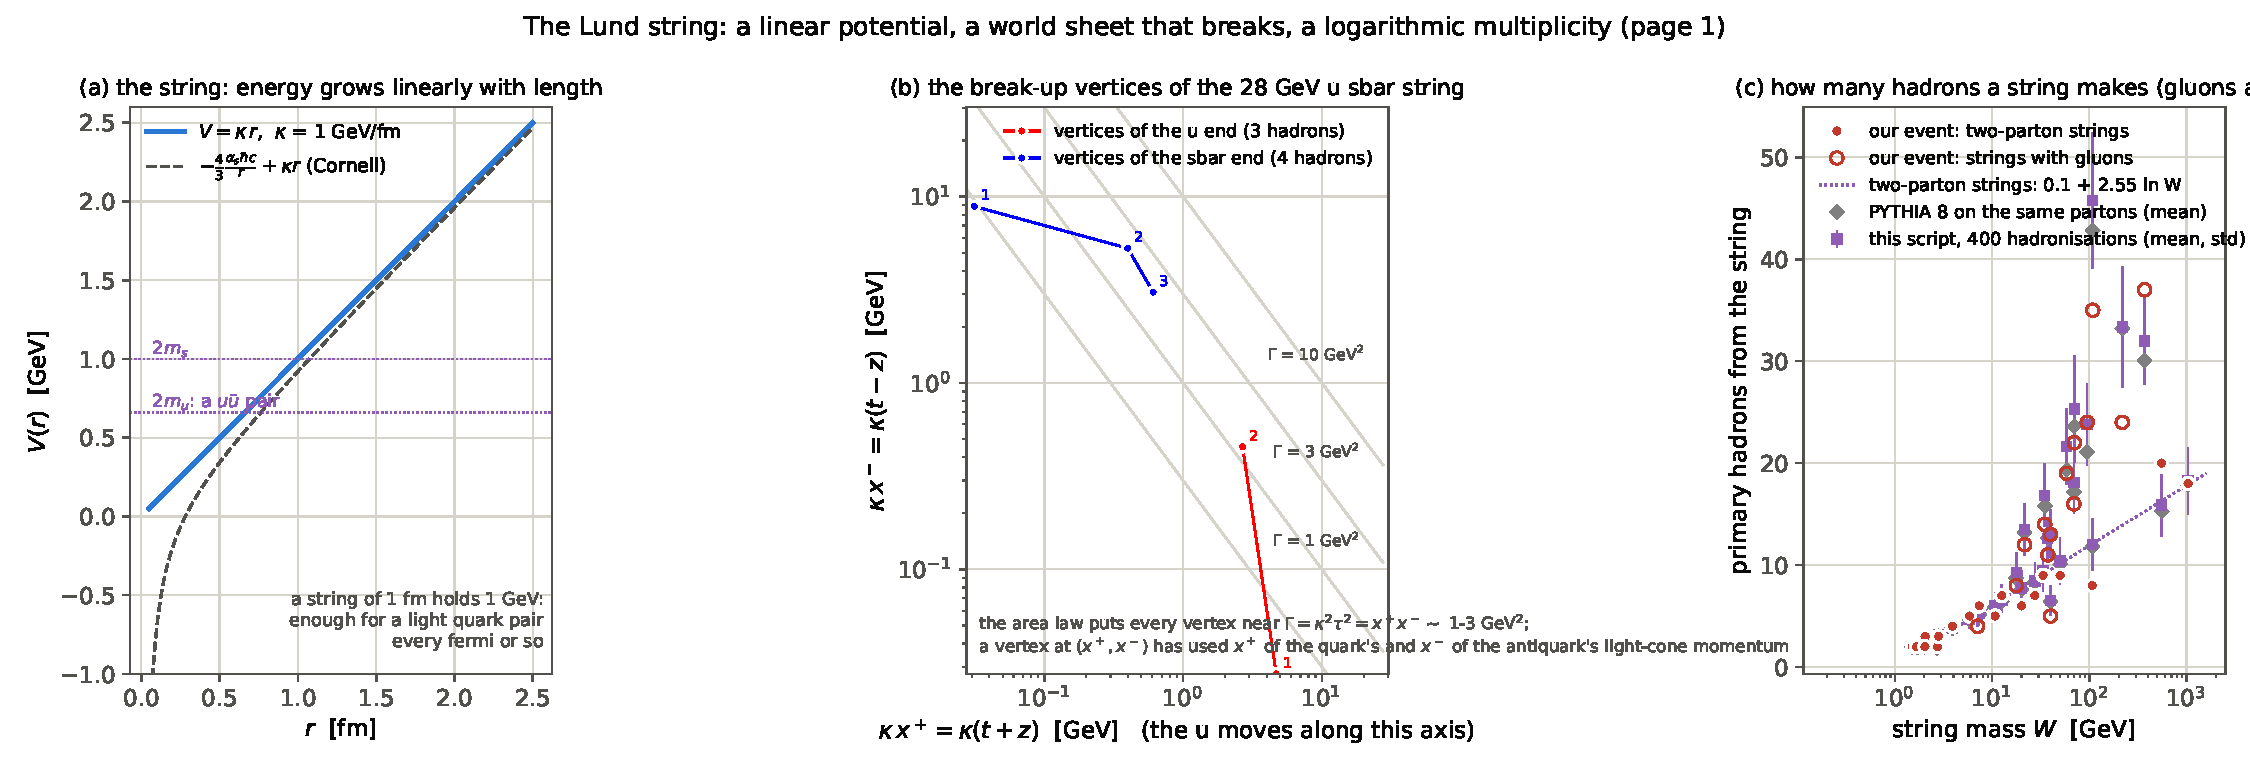
\includegraphics[page=1,width=\textwidth]{Had/Standalone/theory_hadronisation.pdf}
\caption[The linear potential, the break-up vertices and the multiplicity]{Page~1
of \file{theory_hadronisation.pdf}. (a) The linear potential of
\cref{eq:children_getting_married:potential} against the Cornell form
with a Coulomb term, and the energy of a $1\,\mathrm{fm}$ string against
the mass of a light-quark pair. (b) The break-up vertices of the $27.5\GeV$
two-parton string of our event in light-cone coordinates, from the two
ends, with the hyperbolae of constant $\Gamma$. (c) The number of primary
hadrons of every string of our event against its mass, with the ensemble
means of the script and of \PYTHIA on the same partons, and the logarithmic
fit for two-parton strings; strings with gluons lie above it.}
\label{fig:children_getting_married:string_plot}
\end{figure}

\subsubsection{How the rope snaps: tunnelling, flavours and transverse momentum}
\label{sec:children_getting_married:breakup}

First the bookkeeping of a break, then its mechanism.
\Cref{fig:children_getting_married:chain_sketch} follows the mother's
rope break by break as the \code{-v} log recorded it, with the gluon kinks
left out of the drawing. A break at the $\bar u$ end creates a $u\bar u$
pair: the new $u$ joins the old $\bar u$ into a $\pi^0$ ($u\bar u$), which
leaves, and the new $\bar u$ is the end of what is left. A break at the
$b$ end creates a $d\bar d$ pair: the new $\bar d$ joins the mother into
the \Bstarbar ($b\bar d$), so that the original $b$ sits in the first
hadron of the chain after one break, and the new $d$ is the end. A diquark
pair $(sd)(\overline{sd})$ makes an antibaryon, $\bar\Sigma^0$
($\bar u\bar d\bar s$), and leaves a diquark end that the next break must
turn into the baryon partner, $\Sigma^0$ ($uds$). The two ends take turns
in random order; after fourteen hadrons the remaining $1.2\GeV$ is below
the stopping mass, one last $d\bar d$ pair is created, and the final two
hadrons share what is left. The result, the bottom row of the figure, is a
chain of sixteen hadrons with fifteen vacuum pairs between neighbours: the
quark of each pair went into the hadron on one side, the antiquark into
the hadron on the other, the original $b$ is in the first hadron, the
original $\bar u$ in the last, and every quark in between was created at a
break. Flavour, charge and baryon number are conserved at every step
because the pairs are neutral in all three.

\begin{figure}[htbp]\centering
\resizebox{\textwidth}{!}{% ---------------------------------------------------------------------------
% The rope snaps, break by break: the b quark's string of our event (the -v
% log, string 1), with the gluon kinks left out of the drawing. Each row is
% the string that is left, the end that fires and the pair that appears; the
% peeled-off hadrons accumulate on the left (from the b end) and on the right
% (from the ubar end). The last row is the full chain of sixteen with the
% vacuum pair written between every two neighbours: the quark of each pair
% went into the hadron on its right, the antiquark into the one on its left.
% ---------------------------------------------------------------------------
\begin{tikzpicture}[x=1cm,y=1cm,
  every node/.style={font=\footnotesize},
  q/.style={circle,inner sep=0pt,minimum size=2.2mm,fill=red!80!black},
  aq/.style={circle,inner sep=0pt,minimum size=2.2mm,fill=blue!80!black},
  nq/.style={circle,inner sep=0pt,minimum size=2.0mm,fill=green!50!black},
  naq/.style={circle,inner sep=0pt,minimum size=2.0mm,fill=green!50!black,draw=black,line width=0.5pt},
  rope/.style={orange!80!black,line width=2.0pt},
  hb/.style={rounded corners=2pt,draw=red!70!black,fill=red!8,minimum width=9.6mm,minimum height=7mm,inner sep=1pt,align=center,font=\scriptsize},
  hu/.style={rounded corners=2pt,draw=blue!70!black,fill=blue!8,minimum width=9.6mm,minimum height=7mm,inner sep=1pt,align=center,font=\scriptsize},
  hf/.style={rounded corners=2pt,draw=black!60,fill=black!6,minimum width=9.6mm,minimum height=7mm,inner sep=1pt,align=center,font=\scriptsize},
  lab/.style={font=\scriptsize,align=center},
  tiny/.style={font=\tiny,align=center},
  head/.style={font=\small\bfseries}]
% a row: \chainrow{y}{half length}{left end label}{right end label}{W text}
\def\chainrow#1#2#3#4#5{\draw[rope] (-#2,#1) -- (#2,#1);
  \node[lab,anchor=south] at (-#2,#1+0.12) {#3}; \node[lab,anchor=south] at (#2,#1+0.12) {#4};
  \node[lab,anchor=west,text=black!65] at (7.3,#1) {#5};}
% ---- row 0: the string as the shower left it
\node[head,anchor=west] at (-9.6,8.15) {the mother's rope, break by break (string~1 of the record; the four gluon kinks are left out of the drawing)};
\chainrow{7.4}{4.1}{$b$}{$\bar u$}{$W=69.3\GeV$}
\node[q] at (-4.1,7.4) {}; \node[aq] at (4.1,7.4) {};
\node[lab,anchor=east,text=black!65] at (-7.3,7.4) {the string the shower\\ and the cousins left};
% ---- row 1: ubar end, pair u ubar -> pi0
\chainrow{6.3}{4.1}{$b$}{$\bar u$}{$68.8$}
\node[q] at (-4.1,6.3) {}; \node[naq] at (4.1,6.3) {};
\node[hu,anchor=west] at (4.35,6.3) {\phantom{$\pi^0$}}; \node[nq] at (4.55,6.3) {}; \node[aq] at (4.95,6.3) {};
\node[tiny,anchor=south] at (4.75,6.52) {$\pi^0\ (u\bar u)$};
\node[lab,anchor=east,text=black!65] at (-7.3,6.3) {$\bar u$ end fires: a $u\bar u$ pair;\\ the new $u$ joins the old $\bar u$};
% ---- row 2: b end, pair d dbar -> B*bar0
\chainrow{5.2}{2.6}{$d$}{$\bar u$}{$29.0$}
\node[nq] at (-2.6,5.2) {}; \node[naq] at (2.6,5.2) {};
\node[hb,anchor=east] at (-2.85,5.2) {\phantom{$\bar B^{*0}$}}; \node[q] at (-3.45,5.2) {}; \node[naq] at (-3.05,5.2) {};
\node[tiny,anchor=south] at (-3.25,5.42) {$\bar B^{*0}\ (b\bar d)$};
\node[hu,anchor=west] at (2.85,5.2) {$\pi^0$};
\node[lab,anchor=east,text=black!65] at (-7.3,5.2) {$b$ end fires: a $d\bar d$ pair;\\ the mother is already married};
% ---- row 3: ubar end, diquark pair -> Sigmabar0
\chainrow{4.1}{2.45}{$d$}{$sd$}{$26.0$}
\node[nq] at (-2.45,4.1) {}; \node[nq] at (2.45,4.1) {};
\node[hb,anchor=east] at (-2.7,4.1) {$\bar B^{*0}$};
\node[hu,anchor=west] at (2.7,4.1) {\phantom{$\bar\Sigma^0$}}; \node[aq] at (2.95,4.1) {}; \node[naq] at (3.25,4.1) {}; \node[naq] at (3.55,4.1) {};
\node[tiny,anchor=south] at (3.25,4.32) {$\bar\Sigma^0\ (\bar u\bar d\bar s)$};
\node[hu,anchor=west] at (3.8,4.1) {$\pi^0$};
\node[lab,anchor=east,text=black!65] at (-7.3,4.1) {$\bar u$ end: a diquark pair $(sd)(\overline{sd})$;\\ an antibaryon, and a diquark end};
% ---- row 4: ubar end, pair u ubar -> Sigma0
\chainrow{3.0}{2.3}{$d$}{$\bar u$}{$21.4$}
\node[nq] at (-2.3,3.0) {}; \node[naq] at (2.3,3.0) {};
\node[hb,anchor=east] at (-2.55,3.0) {$\bar B^{*0}$};
\node[hu,anchor=west] at (2.55,3.0) {\phantom{$\Sigma^0$}}; \node[nq] at (2.8,3.0) {}; \node[nq] at (3.1,3.0) {}; \node[nq] at (3.4,3.0) {};
\node[tiny,anchor=south] at (3.1,3.22) {$\Sigma^0\ (uds)$};
\node[hu,anchor=west] at (3.65,3.0) {$\bar\Sigma^0$}; \node[hu,anchor=west] at (4.75,3.0) {$\pi^0$};
\node[lab,anchor=east,text=black!65] at (-7.3,3.0) {$\bar u$ end: a $u\bar u$ pair; the $u$ joins\\ the diquark, the baryon partner};
% ---- row 5: ubar end, pair d dbar -> pi-
\chainrow{1.9}{2.2}{$d$}{$\bar d$}{$20.3$}
\node[nq] at (-2.2,1.9) {}; \node[naq] at (2.2,1.9) {};
\node[hb,anchor=east] at (-2.45,1.9) {$\bar B^{*0}$};
\node[hu,anchor=west] at (2.45,1.9) {\phantom{$\pi^-$}}; \node[nq] at (2.75,1.9) {}; \node[naq] at (3.15,1.9) {};
\node[tiny,anchor=south] at (2.95,2.12) {$\pi^-\ (d\bar u)$};
\node[hu,anchor=west] at (3.55,1.9) {$\Sigma^0$}; \node[hu,anchor=west] at (4.65,1.9) {$\bar\Sigma^0$}; \node[hu,anchor=west] at (5.75,1.9) {$\pi^0$};
\node[lab,anchor=east,text=black!65] at (-7.3,1.9) {$\bar u$ end: a $d\bar d$ pair};
% ---- row 6: b end, pair d dbar -> eta'
\chainrow{0.8}{1.9}{$d$}{$\bar d$}{$13.9$}
\node[nq] at (-1.9,0.8) {}; \node[naq] at (1.9,0.8) {};
\node[hb,anchor=east] at (-2.15,0.8) {\phantom{$\eta'$}}; \node[nq] at (-2.75,0.8) {}; \node[naq] at (-2.35,0.8) {};
\node[tiny,anchor=south] at (-2.55,1.02) {$\eta'\ (d\bar d)$};
\node[hb,anchor=east] at (-3.25,0.8) {$\bar B^{*0}$};
\node[hu,anchor=west] at (2.15,0.8) {$\pi^-$}; \node[hu,anchor=west] at (3.25,0.8) {$\Sigma^0$}; \node[hu,anchor=west] at (4.35,0.8) {$\bar\Sigma^0$}; \node[hu,anchor=west] at (5.45,0.8) {$\pi^0$};
\node[lab,anchor=east,text=black!65] at (-7.3,0.8) {$b$ end: a $d\bar d$ pair, and the\\ $\eta'$ forms across the first kink};
% ---- row 7: dots
\node[lab,text=black!65] at (0,-0.1) {$\vdots$\quad eight more hadrons, five from the $b$ end and three from the $\bar u$ end, in the random order the script drew; $W$ falls from $13.9$ to $1.2\GeV$\quad$\vdots$};
% ---- row 8: the final two
\chainrow{-1.0}{0.9}{$u$}{$\bar u$}{$1.2<\Wmin=3.0\GeV$: the last pair}
\node[nq] at (-0.9,-1.0) {}; \node[naq] at (0.9,-1.0) {};
\node[naq] at (-0.2,-1.0) {}; \node[nq] at (0.2,-1.0) {}; \node[tiny,text=green!40!black,anchor=south] at (0,-0.85) {$\bar d\ d$};
\node[lab,anchor=east,text=black!65] at (-7.3,-1.0) {the two chains are joined: one last\\ $d\bar d$ pair, and two hadrons share $1.2\GeV$};
\foreach \x/\n in {-1.65/{$\pi^-$},-2.75/{$\pi^0$},-3.85/{$\rho^+$},-4.95/{$\pi^0$},-6.05/{$\rho^-$}} {\node[hb,anchor=east] at (\x,-1.0) {\n};}
\foreach \x/\n in {1.65/{$K^+$},2.75/{$\bar K^{*0}$},3.85/{$\pi^0$},4.95/{$\pi^-$},6.05/{$\Sigma^0$}} {\node[hu,anchor=west] at (\x,-1.0) {\n};}
\node[lab,text=black!65] at (-7.05,-1.0) {$\cdots$}; \node[lab,text=black!65] at (7.05,-1.0) {$\cdots$};
% ---- row 9: the chain of sixteen with the pairs between neighbours
\node[head,anchor=west] at (-9.6,-2.1) {the chain: sixteen hadrons, fifteen vacuum pairs between neighbours (the quark of each pair went right, the antiquark left)};
\def\chainbox#1#2#3#4{\node[#4] at (#1*1.1-8.25,-3.0) {#2\\[-1pt] {\tiny #3}};}
\chainbox{0}{$\bar B^{*0}$}{$b\bar d$}{hb}
\chainbox{1}{$\eta'$}{$d\bar d$}{hb}
\chainbox{2}{$\rho^-$}{$d\bar u$}{hb}
\chainbox{3}{$\pi^0$}{$u\bar u$}{hb}
\chainbox{4}{$\rho^+$}{$u\bar d$}{hb}
\chainbox{5}{$\pi^0$}{$d\bar d$}{hb}
\chainbox{6}{$\pi^-$}{$d\bar u$}{hb}
\chainbox{7}{$\rho^+$}{$u\bar d$}{hf}
\chainbox{8}{$\pi^-$}{$d\bar u$}{hf}
\chainbox{9}{$K^+$}{$u\bar s$}{hu}
\chainbox{10}{$\bar K^{*0}$}{$s\bar d$}{hu}
\chainbox{11}{$\pi^0$}{$d\bar d$}{hu}
\chainbox{12}{$\pi^-$}{$d\bar u$}{hu}
\chainbox{13}{$\Sigma^0$}{$uds$}{hu}
\chainbox{14}{$\bar\Sigma^0$}{$\bar u\bar d\bar s$}{hu}
\chainbox{15}{$\pi^0$}{$u\bar u$}{hu}
\foreach \i/\p in {0/{$d\bar d$},1/{$d\bar d$},2/{$u\bar u$},3/{$u\bar u$},4/{$d\bar d$},5/{$d\bar d$},6/{$u\bar u$},7/{$d\bar d$},8/{$u\bar u$},9/{$s\bar s$},10/{$d\bar d$},11/{$d\bar d$},12/{$u\bar u$},13/{$(sd)(\overline{sd})$},14/{$u\bar u$}} {
  \node[tiny,text=green!40!black,anchor=north] at (\i*1.1-7.7,-3.42) {\p};}
\draw[decorate,decoration={brace,mirror,amplitude=3pt}] (-8.7,-3.75) -- (-7.8,-3.75) node[midway,below=3pt,lab] {holds the\\ mother's $b$};
\draw[decorate,decoration={brace,mirror,amplitude=3pt}] (7.8,-3.75) -- (8.7,-3.75) node[midway,below=3pt,lab] {holds the\\ original $\bar u$};
\draw[decorate,decoration={brace,mirror,amplitude=3pt}] (-7.6,-3.75) -- (-0.15,-3.75) node[midway,below=3pt,lab] {from the $b$ end, in the order the $b$ end made them};
\draw[decorate,decoration={brace,mirror,amplitude=3pt}] (-0.05,-3.75) -- (0.95,-3.75) node[midway,below=3pt,lab] {the final two};
\draw[decorate,decoration={brace,mirror,amplitude=3pt}] (1.05,-3.75) -- (7.6,-3.75) node[midway,below=3pt,lab] {from the $\bar u$ end};
\end{tikzpicture}
}
\caption[The mother's rope break by break]{The mother's rope break by
break, string~1 of the \code{-v} log, with the four gluon kinks left out
of the drawing. Each row is the string that is left, the end that fires,
the pair that appears and the hadron that leaves, red from the $b$ end and
blue from the $\bar u$ end, with the remaining invariant mass on the
right; eight hadrons are skipped between the sixth break and the final
two. The bottom row is the chain of sixteen in their order along the rope,
each with its quark content, and between every two neighbours the vacuum
pair they share: the original $b$ is in the first hadron, the original
$\bar u$ in the last.}
\label{fig:children_getting_married:chain_sketch}
\end{figure}

Guess first: the string breaks by creating a quark--antiquark pair. Which
flavour? The energy is there for any of them, a $28\GeV$ string could pay
for a $b\bar b$ pair three times over, and yet no $b$ quark has ever come
out of a string. The reason is the \emph{mechanism}
(\cref{fig:children_getting_married:breakup_sketch}): the pair is created
at a point, where the field has no energy to give it, and the two quarks
must separate to a distance $2\mT/\kappa$ before the field energy between
them equals their transverse mass. That is a classically forbidden step,
and its probability is the tunnelling factor of Schwinger pair production
in a constant field~\cite{Casher:1978wy},
\begin{equation}
  P\propto\exp\!\left(-\frac{\pi\mT^2}{\kappa}\right)
  =\exp\!\left(-\frac{\pi m^2}{\kappa}\right)\exp\!\left(-\frac{\pi\pt^2}{\kappa}\right),
  \qquad \mT^2=m^2+\pt^2,
  \label{eq:children_getting_married:tunnelling}
\end{equation}
which does three jobs at once. It suppresses heavy flavours: with the
constituent masses $m_{u,d}=0.33$ and $m_s=0.5\GeV$ the ratio
$s/u=\exp[-\pi(m_s^2-m_u^2)/\kappa]$ is $0.106$, charm is below $10^{-10}$
and bottom unreachable. It gives every break a transverse momentum,
Gaussian with $\sigma^2=\kappa/2\pi$ per component, $0.18\GeV$, with the
quark and the antiquark of the pair taking $\pm\vec p_{\mathrm{T}}$ so that
a hadron's transverse momentum is the sum of the kicks of its two
constituents. And it makes baryons rare: a diquark--antidiquark pair, which
is how a string makes a baryon and an antibaryon next to each other, is
heavier and tunnels less. The model keeps the structure and lets the data
set the sizes: $s/u=0.217$ rather than $0.106$, because constituent masses
are not the masses the formula wants; $\sigma=0.335\GeV$ for the pair,
$0.237$ per component, rather than $0.18$, because gluon radiation below
the shower's cut-off ends up here; the diquark weight $0.081$ with the
strange-diquark and spin-$1$ suppressions $0.915$ and $3\times0.0275$. The
new quark then joins the old end into a hadron, and spin counting does the
rest: a vector meson with probability $V/(1+V)$, where $V$ is $0.5$ for
$u,d$, $0.55$ for $s$, $0.88$ for $c$ and $2.2$ for $b$, the heavy ones
higher because the hyperfine splitting that favours the pseudoscalar shrinks
with the quark mass; $u\bar u$, $d\bar d$ and $s\bar s$ mixed into $\pi^0$
($(u\bar u-d\bar d)/\sqrt2$), $\eta$ and $\eta'$ (the two mixtures of
$u\bar u+d\bar d$ with $s\bar s$) with the extra suppressions $0.6$ and $0.12$; and the
SU(6) weights for the octet and decuplet baryons.

\begin{figure}[htbp]\centering
\resizebox{\textwidth}{!}{% ---------------------------------------------------------------------------
% The break-up. (a) A q' qbar' pair created in the field has to tunnel apart
% to a distance 2 m_T/kappa before it is on shell: the probability is
% exp(-pi m_T^2/kappa), which suppresses strange quarks, kills charm and
% bottom, and gives every break a Gaussian transverse momentum. (b) The
% relative rates of the tune (the -v log, "setting the scene") against the
% tunnelling formula with constituent masses. (c) The pair becomes a hadron
% with its neighbour: spin counting fixes vector against pseudoscalar, and
% a diquark pair makes a baryon and an antibaryon next to each other.
% ---------------------------------------------------------------------------
\begin{tikzpicture}[x=1cm,y=1cm,
  every node/.style={font=\footnotesize},
  q/.style={circle,inner sep=0pt,minimum size=2.2mm,fill=red!80!black},
  aq/.style={circle,inner sep=0pt,minimum size=2.2mm,fill=blue!80!black},
  nq/.style={circle,inner sep=0pt,minimum size=2.2mm,fill=green!50!black},
  naq/.style={circle,inner sep=0pt,minimum size=2.2mm,fill=green!50!black,draw=black},
  lab/.style={font=\scriptsize,align=center},
  head/.style={font=\small\bfseries}]
% ---------------- (a) tunnelling ----------------------------------------------------------------
\begin{scope}
\node[head,anchor=west] at (-0.3,3.4) {(a) a pair tunnels out of the field};
\fill[orange!35] (0.3,2.35) rectangle (5.2,2.65);
\node[q] at (0.2,2.5) {}; \node[aq] at (5.3,2.5) {};
\node[lab] at (0.2,2.9) {$q$}; \node[lab] at (5.3,2.9) {$\bar q$};
\node[lab,text=black!65] at (2.75,2.05) {before: one string, energy $\kappa r$};
\fill[orange!35] (0.3,0.95) rectangle (2.1,1.25);
\fill[orange!35] (3.4,0.95) rectangle (5.2,1.25);
\node[q] at (0.2,1.1) {}; \node[aq] at (5.3,1.1) {};
\node[naq] at (2.2,1.1) {}; \node[nq] at (3.3,1.1) {};
\node[lab,text=green!40!black] at (2.2,1.5) {$\bar q'$}; \node[lab,text=green!40!black] at (3.3,1.5) {$q'$};
\draw[{Stealth}-{Stealth},thin] (2.3,0.75) -- (3.2,0.75) node[midway,below,lab] {$2m_{\mathrm{T}}/\kappa$: the field energy\\ that became the pair's mass};
\node[lab,anchor=north,text width=5.4cm] at (2.75,-0.05) {the pair is born at a point with $m_{\mathrm{T}}^2=m^2+p_{\mathrm{T}}^2$ and must separate before it is on shell: a classically forbidden step,\\ $P\propto\exp(-\pi m_{\mathrm{T}}^2/\kappa)=\exp(-\pi m^2/\kappa)\,\exp(-\pi p_{\mathrm{T}}^2/\kappa)$};
\end{scope}
% ---------------- (b) the rates ----------------------------------------------------------------
\begin{scope}[xshift=6.9cm]
\node[head,anchor=west] at (-0.3,3.4) {(b) who comes out of the vacuum};
\draw[-{Stealth}] (0,-0.2) -- (0,3.0) node[left,lab] {rate};
\draw (0,-0.2) -- (5.6,-0.2);
% bars: u 1, d 1, s 0.217, diquark 0.081, c ~0 (log scale would hide the point; linear here)
\foreach \x/\h/\n/\t in {0.5/2.6/$u$/{1}, 1.5/2.6/$d$/{1}, 2.5/0.56/$s$/{0.217}, 3.5/0.21/$qq$/{0.081}, 4.5/0.02/$c$/{$<10^{-10}$}} {
  \fill[teal!60] (\x-0.3,-0.2) rectangle (\x+0.3,-0.2+\h);
  \node[lab,anchor=north] at (\x,-0.3) {\n};
  \node[lab,anchor=south] at (\x,-0.2+\h) {\t};}
\node[lab,anchor=north west,text width=5.3cm,text=black!65] at (-0.2,-0.85) {tunnelling with $m_u=0.33$, $m_s=0.5\GeV$: $s/u=\exp(-\pi(m_s^2-m_u^2)/\kappa)=0.106$; the tune needs $0.217$, because constituent masses are not the right masses to use. $c$ and $b$ never come from the vacuum: every heavy quark of the event is from the hard process, the showers or the secondary scatterings};
\end{scope}
% ---------------- (c) the hadron ---------------------------------------------------------------
\begin{scope}[xshift=13.5cm]
\node[head,anchor=west] at (-0.3,3.4) {(c) the pair becomes a hadron};
\node[lab,anchor=north west,text width=4.9cm] at (-0.3,3.05) {
\textbf{meson} $q\bar q'$: spin $0$ or $1$; the tune's vector weight $V/(1+V)$\\
$u,d$: $0.5/1.5=0.33$ \quad $s$: $0.355$ \quad $b$: $2.2/3.2=0.69$\\
$u\bar u$, $d\bar d$, $s\bar s$ mix into $\pi^0$, $\eta$, $\eta'$ ($\eta\times0.6$, $\eta'\times0.12$)\\[3pt]
\textbf{baryon}: the vacuum pair is a diquark pair $(qq)(\overline{qq})$ with $P=0.081/1.081=0.075$; the diquark joins the next quark and SU(6) counts the octet and decuplet states:\\ $sd_0+u\to\Lambda^0$ $0.125$, $\Sigma^0$ $0.375$ (the rest is rejected and a new flavour drawn)\\[3pt]
\textbf{transverse momentum}: the pair gets $\pm\vec p_{\mathrm{T}}$, each component Gaussian with $\sigma/\sqrt2=0.237\GeV$; a hadron's $\vec p_{\mathrm{T}}$ is the sum of its two quarks' kicks};
\end{scope}
\end{tikzpicture}
}
\caption[The break-up: tunnelling, flavour weights and hadron
multiplets]{Left: a pair created at a point has to tunnel apart before it
is on shell, \cref{eq:children_getting_married:tunnelling}. Middle: the
relative rates of the flavours in the tune against the tunnelling formula.
Right: how the new quark and the old end become a hadron, with the
numbers of the \code{-v} log.}
\label{fig:children_getting_married:breakup_sketch}
\end{figure}

\paragraph{The numbers.} The first hadron of the $b$ quark's string is
drawn from the $\bar u$ end. The log prints the flavour draw, a quark
rather than a diquark with $P=1/(1+0.081)=0.925$, then $u$ among
$d:u:s=1:1:0.217$; the hadron, $u\bar u$ with the pseudoscalar chosen with
$1/2$ and $\pi^0$ among the $\pi^0$, $\eta$, $\eta'$ mixtures with weights
$0.5$, $0.296$, $0.204$; and the kick, $(-0.603,-0.143)\GeV$ from the
Gaussian of width $0.237$, a $2.5\sigma$ draw in $p_x$, which gives the pion
$\mT=0.634\GeV$. Two hadrons later the diquark branch fires with its
$P=0.075$: an $sd_0$ antidiquark, the SU(6) weights $\Lambda^0$ ($uds$,
isospin $0$) $0.125$ and $\Sigma^0$ ($uds$, isospin $1$) $0.375$ (the rest
of the unit weight means ``reject and draw a new flavour''), a
$\bar\Sigma^0$ ($\bar u\bar d\bar s$), and the next hadron from that end
must be its baryon partner, $\Sigma^0$. The $b$ end draws $\bar d$ and a vector
with $P=2.2/3.2=0.688$: \Bstarbar. Over the whole event the 365 hadrons are
125 pions, 65 $\rho$, 20 $\omega$ (the spin-1 $u\bar u+d\bar d$), 17
$\eta$, 50 kaons, 25 $K^*$ (the spin-1 kaons) and 52 baryons, 94 with strangeness; \PYTHIA on the same partons makes $38\%$ pions, $18\%$
$\rho$, $6\%$ $\omega$, $5\%$ $\eta$, $12\%$ kaons and $6\%$ $K^*$, and
panel~(c) of \cref{fig:children_getting_married:breakup_plot} puts the two
side by side. The 580 kick components of the event have a root mean
square of $0.231\GeV$ against the $0.237$ of the input, and the hadrons'
$\langle\pt^2\rangle$ relative to the string is $2\sigma^2=0.224\GeV^2$.

\begin{figure}[htbp]\centering
\includegraphics[page=2,width=\textwidth]{Had/Standalone/theory_hadronisation.pdf}
\caption[Tunnelling, the transverse kicks and the species]{Page~2 of
\file{theory_hadronisation.pdf}. (a) The tunnelling factor of
\cref{eq:children_getting_married:tunnelling} against the mass of the
pair's quark or diquark, with the tune's $s/u$ and diquark weights marked.
(b) The $p_x$ and $p_y$ components of every break-up kick of our event
against the Gaussian of the tune. (c) The species of the primary hadrons:
our event, the script's 400 hadronisations and \PYTHIA's on the same
partons.}
\label{fig:children_getting_married:breakup_plot}
\end{figure}

\subsubsection{Who takes how much: the fragmentation function and the iteration from both ends}
\label{sec:children_getting_married:fragmentation_function}

Guess first: the $b$ quark's string has $69\GeV$ of mass and will make
sixteen hadrons. How is the momentum shared? Not equally, and not in any
order of rank: the area law of \cref{eq:children_getting_married:area_law}
fixes the answer, and the way to use it is to produce the hadrons
iteratively from the two ends in random order, each taking a fraction $z$
of the remaining light-cone momentum of its end,
$p^+_{\mathrm{had}}=z\,p^+_{\mathrm{rem}}$ for a hadron from the $+$ end,
with the other light-cone component fixed by its mass shell,
$p^-_{\mathrm{had}}=\mT^2/p^+_{\mathrm{had}}$. The area law translated
into $z$ is the Lund symmetric fragmentation
function~\cite{Andersson:1983jt},
\begin{equation}
  f(z)\propto\frac{1}{z}\,z^{a_{\mathrm{old}}}\left(\frac{1-z}{z}\right)^{a_{\mathrm{new}}}
  \exp\!\left(-\frac{b\,\mT^2}{z}\right)
  \;\xrightarrow{\;a_{\mathrm{old}}=a_{\mathrm{new}}=a\;}\;
  \frac{1}{z}(1-z)^a\exp\!\left(-\frac{b\,\mT^2}{z}\right),
  \label{eq:children_getting_married:lund}
\end{equation}
``symmetric'' because it gives the same hadrons whether the chain is
started from the quark end or from the antiquark end, which is what forced
this form and no other; $a_{\mathrm{old}}$ and $a_{\mathrm{new}}$ are the
$a$ parameters of the flavour at the end and of the new flavour, equal for
quarks and larger by $0.97$ for a diquark. The exponential is the area law
with the hadron's own area $\mT^2/z$ in it, and it is what makes heavy
hadrons take large $z$: a $\rho$ takes $0.53$ of its end's momentum on
average, a pion $0.33$. After each hadron the vertex moves out along the
string, and its proper time follows from the previous one by
\begin{equation}
  \Gamma_{\mathrm{new}}=(1-z)\left(\Gamma_{\mathrm{old}}+\frac{\mT^2}{z}\right),
  \label{eq:children_getting_married:gamma_step}
\end{equation}
with $\Gamma=0$ at the ends. The iteration cannot go on for ever: when the
invariant mass of what is left between the two current ends falls below
\begin{equation}
  \Wmin=m_{q_1}+m_{q_2}+\mathrm{stopMass}+\mathrm{stopNewFlav}\;m_{q_{\mathrm{last}}}
  =m_{q_1}+m_{q_2}+1.0+2.0\,m_{q_{\mathrm{last}}},
  \label{eq:children_getting_married:wmin}
\end{equation}
smeared by $\pm20\%$ so that the stop does not leave a scar in the
spectrum, the two chains are joined: one last pair is created, the two
final hadrons share what is left with the transverse momentum of that
break, and the orientation along the string, which hadron goes forward, is
drawn with the product of the two ends' fragmentation functions. If no
hadron fits at all the string is restarted with new random numbers.

\begin{figure}[htbp]\centering
\resizebox{\textwidth}{!}{% ---------------------------------------------------------------------------
% The iteration from both ends, drawn with the b quark's string of our event
% (the -v log, "string 1: W = 69.34 GeV, 6 partons"). Each bar is the string
% that is left; the + end (the b) eats from the left, the - end (the ubar)
% from the right; the piece removed at each step is the hadron, red when it
% comes from the b end and blue from the other end. The widths are the
% drops of the remaining invariant mass W, so the picture is schematic:
% W is not additive, but it falls monotonically to W_min.
% ---------------------------------------------------------------------------
\begin{tikzpicture}[x=1cm,y=1cm,
  every node/.style={font=\footnotesize},
  lab/.style={font=\scriptsize,align=left,anchor=west},
  head/.style={font=\small\bfseries}]
\node[head,anchor=west] at (0,0.75) {the $b$ quark's string, $W=69.34\GeV$, $b\,g\,g\,g\,g\,\bar u$: hadrons from both ends until $W<W_{\min}$};
\node[lab,anchor=east] at (-0.1,0.3) {$b$ (+ end)};
\node[lab,anchor=west] at (8.1,0.3) {$\bar u$ ($-$ end)};
\draw[-{Stealth},thin] (-0.05,0.1) -- (-0.05,-5.9) node[below,font=\scriptsize] {production order};
% scale: 69.34 GeV = 8 cm -> 0.11537 cm/GeV. L, R in GeV before each step; the eaten piece [Lold,Lnew] or [Rnew,Rold]
% columns: y / Lold / Lnew / Rnew / Rold / colour / label
\foreach \y/\lo/\ln/\rn/\ro/\c/\t in {
 0/0/0/68.79/69.34/blue/{1\; $\pi^0$ from $-$, $z=0.134$, $W\to68.79$},
 1/0/39.74/68.79/68.79/red/{2\; $\bar B^{*0}$ from $+$, Lund--Bowler $z=0.984$, $W\to29.05$},
 2/39.74/39.74/65.77/68.79/blue/{3\; $\bar\Sigma^0$ from $-$ (diquark), $z=0.271$, $W\to26.03$},
 3/39.74/39.74/61.15/65.77/blue/{4\; $\Sigma^0$ from $-$, $z=0.764$, $W\to21.41$},
 4/39.74/39.74/60.07/61.15/blue/{5\; $\pi^-$ from $-$, $z=0.333$, $W\to20.33$},
 5/39.74/46.15/60.07/60.07/red/{6\; $\eta'$ from $+$, $z=0.416$, across a kink, $W\to13.92$},
 6/46.15/46.15/59.35/60.07/blue/{7\; $\pi^0$ from $-$, $z=0.591$, $W\to13.19$},
 7/46.15/46.15/56.56/59.35/blue/{8\; $\bar K^{*0}$ from $-$, $z=0.446$, $W\to10.40$},
 8/46.15/46.15/55.00/56.56/blue/{9\; $K^+$ from $-$, $z=0.565$, $W\to8.84$},
 9/46.15/48.19/55.00/55.00/red/{10\; $\rho^-$ from $+$, $z=0.314$, $W\to6.80$},
 10/48.19/48.53/55.00/55.00/red/{11\; $\pi^0$ from $+$, $z=0.242$, $W\to6.46$},
 11/48.53/50.48/55.00/55.00/red/{12\; $\rho^+$ from $+$, $z=0.444$, $W\to4.51$},
 12/50.48/52.60/55.00/55.00/red/{13\; $\pi^0$ from $+$, $z=0.603$, $W\to2.39$},
 13/52.60/53.78/55.00/55.00/red/{14\; $\pi^-$ from $+$, $z=0.274$, $W\to1.21<W_{\min}=3.00$}} {
  \fill[orange!25] ({0.11537*\lo},{-0.4*\y-0.14}) rectangle ({0.11537*\ro},{-0.4*\y+0.14});
  \fill[\c!70] ({0.11537*\lo},{-0.4*\y-0.14}) rectangle ({0.11537*\ln},{-0.4*\y+0.14});
  \fill[\c!70] ({0.11537*\rn},{-0.4*\y-0.14}) rectangle ({0.11537*\ro},{-0.4*\y+0.14});
  \draw[black!50,thin] ({0.11537*\lo},{-0.4*\y-0.14}) rectangle ({0.11537*\ro},{-0.4*\y+0.14});
  \node[lab] at (8.2,{-0.4*\y}) {\t};}
% the final two
\fill[red!70] ({0.11537*53.78},-5.74) rectangle ({0.11537*54.6},-5.46);
\fill[blue!70] ({0.11537*54.6},-5.74) rectangle ({0.11537*55.0},-5.46);
\draw[black!50,thin] ({0.11537*53.78},-5.74) rectangle ({0.11537*55.0},-5.46);
\node[lab] at (8.2,-5.6) {15, 16\; the final two share $1.21\GeV$: $\rho^+$ ($+$) and $\pi^-$ ($-$), orientation drawn with $P=0.85$};
\node[lab,anchor=north west,text width=15.5cm,font=\scriptsize] at (0,-6.3) {Every step: pick an end at random, draw the new flavour, the hadron, the $p_{\mathrm{T}}$ kick and $z$ from $f(z)$; the hadron takes $z$ of the remaining light-cone momentum on its own side and what its mass needs from the other side; stop when the remaining mass is below $W_{\min}=m_{\mathrm{T},q_1}+m_{\mathrm{T},q_2}+1.0+2.0\,m_{q_{\mathrm{last}}}$ (smeared $\pm20\%$) and give what is left to two hadrons. The $\bar B^{*0}$ took $39.7$ of the $69.3\GeV$ in one step: $x_E=1.004$.};
\end{tikzpicture}
}
\caption[The iteration from both ends on the $b$ quark's string]{The
iteration from both ends on the $b$ quark's string of our event, from the
\code{-v} log: each bar is the string that is left, the $b$ end eats from
the left (red) and the $\bar u$ end from the right (blue), the width of each
bite is the drop of the remaining invariant mass, and the final two share
the $1.21\GeV$ that is below \Wmin.}
\label{fig:children_getting_married:iteration_sketch}
\end{figure}

\paragraph{The numbers.} \Cref{fig:children_getting_married:iteration_sketch}
and the log tell the whole story of string~1, $W=69.34\GeV$,
$b\,g\,g\,g\,g\,\bar u$. The $\bar u$ end goes first: $\pi^0$, $\mT=0.634$,
$b\mT^2=0.394$, $\langle z\rangle=0.452$ from
\cref{eq:children_getting_married:lund}, drawn $z=0.1342$, and
\cref{eq:children_getting_married:gamma_step} gives
$\Gamma=(1-0.1342)(0+0.402/0.1342)=2.595\GeV^2$, a vertex at
$\tau=1.61\,\mathrm{fm}$. Then the $b$ end: \Bstarbar, $\mT=5.332$,
$b\mT^2=27.9$, and the Lund--Bowler function of
\cref{sec:children_getting_married:bowler} with $\langle z\rangle=0.891$;
the draw is $z=0.9843$, $\Gamma=0.453\GeV^2$, and the hadron takes
$166.0$ of the quark's $165.4\GeV$ of energy, more than all of it because
its region reaches into the first gluon. The remaining mass drops from
$68.8$ to $29.0\GeV$ in that one step. Twelve more hadrons follow, with
$z$ between $0.24$ and $0.76$ and $\Gamma$ between $1.1$ and $25\GeV^2$,
until after the fourteenth the remaining $1.209\GeV$ is below
$\Wmin=2.750$ smeared to $2.998\GeV$; the final pair is $d\bar d$, the
final two are a $\rho^+$ ($u\bar d$) from the $b$ side and a $\pi^-$ ($d\bar u$)
from the other,
and the orientation draw, $\ln(f^+f^-)=-1.74$ forward against $-0.02$
reversed, reverses them with $P=0.848$. Sixteen hadrons, momentum
conserved to $10^{-12}\GeV$. Over the whole event the 293 light-flavour
hadrons drew a mean $z$ of $0.486$ against the $0.472$ the functions
predict for their masses, and panel~(c) of
\cref{fig:children_getting_married:fragmentation_plot} shows the remaining
mass of the $b$ string falling step by step towards \Wmin.

\begin{figure}[htbp]\centering
\includegraphics[page=3,width=\textwidth]{Had/Standalone/theory_hadronisation.pdf}
\caption[The Lund function and the iteration on the $b$ quark's string]{Page~3
of \file{theory_hadronisation.pdf}. (a) The Lund symmetric function of
\cref{eq:children_getting_married:lund} for a pion, a $\rho$, a proton from
a diquark end and a kaon from an $s$ end, with their means. (b) The $z$
fractions actually drawn for the light-flavour hadrons of our event against
the expectation. (c) The remaining mass of the $b$ quark's string after
each hadron, red from the $b$ end and blue from the other, and \Wmin of
\cref{eq:children_getting_married:wmin} at each step.}
\label{fig:children_getting_married:fragmentation_plot}
\end{figure}

\subsubsection{Gluons as kinks: regions of the world sheet}
\label{sec:children_getting_married:kinks}

Guess first: the $b$ quark's string has four gluons on it. Does each gluon
make its own jet of hadrons, or do the hadrons follow the string? The
string. A gluon in the Lund model is not a string end but a \emph{kink}, a
point on the string that carries energy and momentum and is pulled by two
string pieces at once, so that it loses its momentum at twice the rate of a
quark end, $2\kappa$~\cite{Andersson:1983ia}. A string
$q\,g_1\,g_2\cdots g_n\,\bar q$ is therefore $n+1$ pieces, and the hadrons
come out along the pieces, between the quark and the first gluon and
between neighbouring gluons, not around each parton: this is the ``string
effect'', the depletion of hadrons between the $q$ and $\bar q$ of a
three-jet event, that JADE saw in 1981 and that the independent
fragmentation of Field and Feynman~\cite{Field:1977fa} could not produce.
The bookkeeping that Sj\"ostrand worked out for it~\cite{Sjostrand:1984ic}
is the hardest part of the script. In the string's frame every parton
contributes a massless light-cone piece, a gluon half of its momentum to
the piece on either side, and the world sheet becomes a set of
\emph{regions} $(i,k)$ spanned by the $p^+$ of piece $i$ from the $q$ side
and the $p^-$ of piece $k$ from the $\bar q$ side, with mass
\begin{equation}
  W_{ik}^2=p_i^+\,p_k^-,
  \qquad
  p_{\mathrm{had}}=\sum_{\text{regions crossed}}
  \left(x^+_{i}\,p_i^+ + x^-_{k}\,p_k^-\right)+\vec p_{\mathrm{T}},
  \label{eq:children_getting_married:regions}
\end{equation}
where the fractions $x^\pm$ are the parts of each piece the hadron
consumes. A hadron that fits in the current region takes $z$ of its own
piece and what its mass needs of the other side; one that does not, because
the region is too light or has been used up, has its vertex placed further
along the string by the proper-time rule, the new vertex being the point at
which \cref{eq:children_getting_married:gamma_step} and the mass shell both
hold, two bilinear equations and a quadratic, scanning first the regions on
the end's own side outwards and then those on the other side. The gluon
halves between the old and the new vertex are swallowed whole, and that is
how a hadron forms \emph{across a kink}, taking momentum from both pieces.
Get this rule wrong, by letting the hadron take $z$ of the current piece
and simply stepping the other side forward, and a hadron with a small $z$
swallows half a gluon that was never its to take: the string ends after
three hadrons with the momentum wrong, a day of my life.

\begin{figure}[htbp]\centering
\resizebox{\textwidth}{!}{% ---------------------------------------------------------------------------
% Gluons as kinks. (a) A q g qbar string: the gluon is a kink that carries
% energy and momentum, pulled by two string pieces; each gluon gives half
% its momentum to the region on either side. (b) The regions of the world
% sheet of the b quark's string (b g g g g ubar): region (i, k) is spanned
% by the light-cone momentum p+ of piece i on the b side and p- of piece k
% on the ubar side; the two ends walk through the regions as they produce
% hadrons (the -v log, "region" lines of string 1).
% ---------------------------------------------------------------------------
\begin{tikzpicture}[x=1cm,y=1cm,
  every node/.style={font=\footnotesize},
  q/.style={circle,inner sep=0pt,minimum size=2.4mm,fill=red!80!black},
  aq/.style={circle,inner sep=0pt,minimum size=2.4mm,fill=blue!80!black},
  g/.style={circle,inner sep=0pt,minimum size=2.2mm,fill=green!50!black},
  lab/.style={font=\scriptsize,align=center},
  head/.style={font=\small\bfseries}]
% ---------------- (a) the kink ------------------------------------------------------------------
\begin{scope}
\node[head,anchor=west] at (-0.3,4.2) {(a) a gluon is a kink on the string};
\node[q] (q) at (0.2,0.6) {}; \node[g] (g) at (2.6,3.0) {}; \node[aq] (aq) at (5.0,0.6) {};
\draw[orange!80!black,line width=2.2pt] (q) -- (g) -- (aq);
\node[lab,below=1pt of q] {$q$}; \node[lab,above=1pt of g,text=green!40!black] {$g$}; \node[lab,below=1pt of aq] {$\bar q$};
\draw[-{Stealth}] (q) -- ++(-0.5,-0.5); \draw[-{Stealth}] (g) -- ++(0,0.6); \draw[-{Stealth}] (aq) -- ++(0.5,-0.5);
\node[lab,text=black!65,anchor=south east] at (1.9,2.65) {piece $q g$:\\ $p_g/2$ from the kink};
\node[lab,text=black!65,anchor=south west] at (3.3,2.65) {piece $g\bar q$:\\ the other $p_g/2$};
\node[lab,anchor=north,text width=5.6cm] at (2.6,0.0) {the kink is pulled by two pieces, force $2\kappa$: it loses its energy twice as fast as a quark end and the string keeps a corner that moves along it. A $q\,g_1\cdots g_n\,\bar q$ string is $n+1$ pieces; a hadron can form across a kink and takes momentum from both pieces};
\end{scope}
% ---------------- (b) the regions ---------------------------------------------------------------
\begin{scope}[xshift=7.6cm,yshift=-0.7cm]
\node[head,anchor=west] at (-0.3,4.9) {(b) the regions of the $b$ quark's string and the two paths};
% grid: i = 0..4 (b side: b, g1/2, g2/2, g3/2, g4/2) horizontal; k = 1..5 (ubar side: g1/2 ... g4/2, ubar) vertical; cells with i < k
\foreach \i in {0,1,2,3,4} {\foreach \k in {1,2,3,4,5} {
  \pgfmathparse{\k > \i ? 1 : 0}
  \ifnum\pgfmathresult=1 \fill[orange!12] (\i*0.8,\k*0.7-0.7) rectangle (\i*0.8+0.8,\k*0.7); \draw[black!30,thin] (\i*0.8,\k*0.7-0.7) rectangle (\i*0.8+0.8,\k*0.7); \fi}}
% visited cells
\foreach \i/\k in {0/1,1/3,2/3} {\fill[red!35] (\i*0.8,\k*0.7-0.7) rectangle (\i*0.8+0.8,\k*0.7);}
\foreach \i/\k in {4/5,3/5,2/4} {\fill[blue!35] (\i*0.8,\k*0.7-0.7) rectangle (\i*0.8+0.8,\k*0.7);}
\foreach \i in {0,1,2,3,4} {\foreach \k in {1,2,3,4,5} {\pgfmathparse{\k > \i ? 1 : 0}\ifnum\pgfmathresult=1 \draw[black!30,thin] (\i*0.8,\k*0.7-0.7) rectangle (\i*0.8+0.8,\k*0.7);\fi}}
% axes labels
\foreach \i/\t in {0/$b$,1/$g_1$,2/$g_2$,3/$g_3$,4/$g_4$} {\node[lab,anchor=north] at (\i*0.8+0.4,-0.05) {\t};}
\node[lab,anchor=north] at (2.0,-0.45) {$i$: the piece on the $b$ side ($p^+$ of parton $i$)};
\foreach \k/\t in {1/$g_1$,2/$g_2$,3/$g_3$,4/$g_4$,5/$\bar u$} {\node[lab,anchor=east] at (-0.1,\k*0.7-0.35) {\t};}
\node[lab,anchor=south,rotate=90] at (-0.75,1.75) {$k$: the piece on the $\bar u$ side ($p^-$ of parton $k$)};
% paths: b end (0,1) -> (1,3) -> (2,3); other end (4,5) -> (3,5) -> (2,4)
\draw[red!80!black,thick,-{Stealth}] (0.4,0.35) -- (1.2,1.75) -- (2.0,1.75);
\draw[blue!80!black,thick,-{Stealth}] (3.6,3.15) -- (2.8,3.15) -- (2.0,2.45);
\node[lab,text=red!80!black,anchor=west] at (0.55,0.2) {$\bar B^{*0}$};
\node[lab,text=red!80!black,anchor=south] at (1.2,1.95) {$\eta'\,\rho^-\,\pi^0$};
\node[lab,text=red!80!black,anchor=north] at (2.0,1.6) {$\rho^+\pi^0\pi^-$};
\node[lab,text=blue!80!black,anchor=south] at (3.6,3.2) {$\pi^0\bar\Sigma^0\Sigma^0\pi^-$};
\node[lab,text=blue!80!black,anchor=south] at (2.75,3.2) {$\pi^0\bar K^{*0}$};
\node[lab,text=blue!80!black,anchor=north] at (2.05,2.3) {$K^+$};
\node[lab,anchor=north west,text width=7.6cm] at (4.3,3.6) {region $(i,k)$ has mass $W_{ik}^2=2\,p_i^+\!\cdot p_k^-$; the $\bar B^{*0}$ formed in $(0,1)$, the $b$ and the first gluon half. The $\eta'$ needed more than $(0,1)$ and $(1,2)$ held: its vertex is placed in $(1,3)$ by the proper-time rule, swallowing the gluon halves in between, which is how a hadron forms across a kink. The two paths meet in $(2,3)$ and $(2,4)$ and the final two share what is left.};
\end{scope}
\end{tikzpicture}
}
\caption[Gluons as kinks and the regions of the $b$ quark's string]{Left:
a gluon is a kink on the string, pulled by two pieces, and gives half its
momentum to each. Right: the regions $(i,k)$ of the world sheet of the $b$
quark's string, $b\,g\,g\,g\,g\,\bar u$, and the paths of the two ends
through them from the \code{-v} log: the \Bstarbar formed in $(0,1)$, the
$\eta'$ jumped to $(1,3)$ across a kink, and the two paths met in $(2,3)$
and $(2,4)$.}
\label{fig:children_getting_married:kinks_sketch}
\end{figure}

\paragraph{The numbers.} The log's ``region'' lines are this subsection,
and \cref{fig:children_getting_married:regions_sketch} draws them as
bites out of the ten pieces. Six partons give five pieces on each side: the $b$ and the four gluon
halves on the $+$ side, the four other halves and the $\bar u$ on the $-$
side. The \Bstarbar formed in region $(0,1)$, the $b$ against the first
gluon's half, taking $0.9843$ of its own piece and $0.9631$ of the other
side's; the first four hadrons from the $\bar u$ end all formed in $(4,5)$.
The sixth hadron, the $\eta'$ from the $b$ end, is the one across a kink:
the log says ``region $(1,3)$, after using up the other side's piece [2]
and its own piece [0]'', so the hadron swallowed what was left of the $b$
piece and the whole of the second gluon's $-$ half, and its vertex was
placed with \cref{eq:children_getting_married:gamma_step} at
$\Gamma=1.600\GeV^2$. The $K^+$ from the other end did the same in $(2,4)$,
swallowing piece 3 on the other side and piece 5 on its own. The two ends
met in $(2,3)$, which the last three hadrons of the $b$ end share, and the
hadrons of the string fill the rapidity range from the $\bar u$ direction
to the $b$ direction without a gap at the gluons (panel~(c) of
\cref{fig:children_getting_married:kinks_plot}). The whole event made
48 joins of this kind's prerequisite, two colour-connected partons closer
than $m_{\mathrm{join}}=0.3\GeV$ in pair mass above their own masses,
which \PYTHIA also makes 48 times on the same partons.

\begin{figure}[htbp]\centering
\resizebox{\textwidth}{!}{% ---------------------------------------------------------------------------
% The numbers of the "region" lines of string 1 (the -v log): how much of
% every light-cone piece each hadron ate. The + side has five pieces, the b
% and the four gluon halves; the - side the other four halves and the ubar.
% Every piece is drawn with unit length (they are not to scale: the b piece
% carries 165 GeV, the ubar piece 7). Red bites are hadrons from the b end,
% which eats the + side from the left and the - side from the left; blue
% bites are hadrons from the ubar end, which eats both from the right; grey
% is what was left for the final two. A hadron whose bites sit in more than
% one piece formed across a kink.
% ---------------------------------------------------------------------------
\begin{tikzpicture}[x=1cm,y=1cm,
  every node/.style={font=\footnotesize},
  lab/.style={font=\scriptsize,align=center},
  tiny/.style={font=\tiny,align=center},
  head/.style={font=\small\bfseries}]
% \pieceat{x0}{y}{list of frac/colour/label}: fills a 3 cm piece from the left
\def\pieceat#1#2#3{\xdef\px{#1}%
  \foreach \f/\c/\l in {#3} {%
    \pgfmathsetmacro{\w}{3*\f}%
    \fill[\c] (\px,#2) rectangle (\px+\w,#2+0.62);%
    \draw[white,line width=0.4pt] (\px,#2) -- (\px,#2+0.62);%
    \pgfmathsetmacro{\xm}{\px+\w/2}%
    \ifdim \w cm > 0.3cm \node[tiny] at (\xm,#2+0.31) {\l}; \fi%
    \pgfmathsetmacro{\nx}{\px+\w}\xdef\px{\nx}}%
  \draw[black!70] (#1,#2) rectangle (#1+3,#2+0.62);}
\colorlet{bA}{red!55!white}\colorlet{bB}{red!40!orange!60}\colorlet{bC}{red!30!white}\colorlet{bD}{red!65!black!50}
\colorlet{uA}{blue!50!white}\colorlet{uB}{blue!35!cyan!60}\colorlet{uC}{blue!25!white}\colorlet{uD}{blue!60!black!50}\colorlet{uE}{cyan!45!white}
\colorlet{fin}{black!22}
% ---------------- the + side -----------------------------------------------------------------------
\node[head,anchor=west] at (0,4.85) {the $+$ side: the $b$ and the four gluon halves, eaten by the $b$ end from the left and by the $\bar u$ end from the right};
\pieceat{0}{3.2}{0.9843/bA/{$\bar B^{*0}$ 0.984}, 0.0157/bB/{}}
\pieceat{3.3}{3.2}{0.3888/bB/{$\eta'$ 0.389}, 0.1919/bC/{$\rho^-$}, 0.1015/bD/{}, 0.3178/bA/{$\rho^+$ 0.32}}
\pieceat{6.6}{3.2}{0.4118/bA/{$\rho^+$ 0.412}, 0.3470/bB/{$\pi^0$ 0.347}, 0.0627/bC/{}, 0.1660/fin/{final}, 0.0125/uE/{}}
\pieceat{9.9}{3.2}{0.0265/uE/{}, 0.9171/uD/{$\bar K^{*0}$ 0.917}, 0.0564/uC/{}}
\pieceat{13.2}{3.2}{0.0228/uC/{}, 0.4048/uB/{$\pi^-$ 0.405}, 0.1328/uA/{$\Sigma^0$}, 0.3118/uB/{$\bar\Sigma^0$ 0.31}, 0.1278/uA/{$\pi^0$}}
\foreach \x/\t in {1.5/{piece 0: the $b$ ($E=165\GeV$)},4.8/{piece 1: $g_1/2$},8.1/{piece 2: $g_2/2$},11.4/{piece 3: $g_3/2$},14.7/{piece 4: $g_4/2$}} {\node[lab,anchor=north] at (\x,3.15) {\t};}
% leaders for the slivers on the + side
\node[tiny,anchor=south,text=red!60!black] at (3.1,3.85) {$\eta'$ ate the\\ last $0.016$};
\draw[thin,red!60!black] (3.1,3.85) -- (3.27,3.6);
\node[tiny,anchor=south,text=red!60!black] at (8.3,3.85) {$\pi^-$ $0.063$, $\rho^-$ $0.19$ in piece 1};
\draw[thin,red!60!black] (8.8,3.85) -- (8.97,3.82);
\node[tiny,anchor=south,text=blue!60!black] at (10.3,4.1) {$K^+$: $0.0125$ of piece 2\\ and the last $0.027$ of piece 3};
\draw[thin,blue!60!black] (9.9,4.1) -- (9.88,3.82); \draw[thin,blue!60!black] (10.0,4.1) -- (9.95,3.82);
\node[tiny,anchor=south,text=blue!60!black] at (14.4,3.85) {$\pi^0$ (5th from $\bar u$): the last\\ $0.056$ of piece 3, $0.023$ of 4};
\draw[thin,blue!60!black] (13.2,3.85) -- (12.82,3.82); \draw[thin,blue!60!black] (13.3,3.85) -- (13.23,3.82);
% ---------------- the - side -----------------------------------------------------------------------
\node[head,anchor=west] at (0,1.95) {the $-$ side: the other four gluon halves and the $\bar u$, eaten the same way};
\pieceat{0}{0.6}{0.9631/bA/{$\bar B^{*0}$ 0.963}, 0.0369/bB/{}}
\pieceat{3.3}{0.6}{1.0/bB/{$\eta'$: the whole piece}}
\pieceat{6.6}{0.6}{0.0103/bB/{}, 0.4932/bC/{$\rho^-$ 0.493}, 0.0786/bD/{}, 0.0183/bA/{}, 0.0051/bB/{}, 0.1245/bC/{$\pi^-$}, 0.27/fin/{final 0.27}}
\pieceat{9.9}{0.6}{0.4971/fin/{final 0.50}, 0.5029/uE/{$K^+$ 0.503}}
\pieceat{13.2}{0.6}{0.0206/uE/{}, 0.0165/uD/{}, 0.0622/uC/{}, 0.0496/uB/{}, 0.4825/uA/{$\Sigma^0$ 0.483}, 0.2344/uB/{$\bar\Sigma^0$}, 0.1342/uA/{$\pi^0$}}
\foreach \x/\t in {1.5/{piece 1: $g_1/2$},4.8/{piece 2: $g_2/2$},8.1/{piece 3: $g_3/2$},11.4/{piece 4: $g_4/2$},14.7/{piece 5: the $\bar u$ ($E=96\GeV$)}} {\node[lab,anchor=north] at (\x,0.55) {\t};}
\node[tiny,anchor=south,text=red!60!black] at (3.1,1.25) {$\eta'$ ate the\\ last $0.037$};
\draw[thin,red!60!black] (3.1,1.25) -- (3.25,1.0);
\node[tiny,anchor=south,text=red!60!black] at (7.5,1.25) {$\eta'$ $0.010$, then $\rho^-$, $\pi^0$ $0.079$, $\rho^+$ $0.018$, $\pi^0$ $0.005$, $\pi^-$ $0.125$};
\draw[thin,red!60!black] (6.65,1.25) -- (6.62,1.0);
\node[tiny,anchor=south,text=blue!60!black] at (13.9,1.25) {$K^+$ $0.021$, $\bar K^{*0}$ $0.017$, $\pi^0$ $0.062$, $\pi^-$ $0.050$};
\draw[thin,blue!60!black] (13.3,1.25) -- (13.3,1.0);
% ---------------- reading --------------------------------------------------------------------------
\node[lab,anchor=north west,text width=16.2cm] at (0,-0.1) {\textcolor{red!60!black}{red}: hadrons from the $b$ end, in order $\bar B^{*0}$, $\eta'$, $\rho^-$, $\pi^0$, $\rho^+$, $\pi^0$, $\pi^-$; \textcolor{blue!60!black}{blue}: from the $\bar u$ end, $\pi^0$, $\bar\Sigma^0$, $\Sigma^0$, $\pi^-$, $\pi^0$, $\bar K^{*0}$, $K^+$; grey: what the final two, $\rho^+$ and $\pi^-$, shared. Every piece is drawn with unit length, which is not to scale: the $b$ end carries $165\GeV$ in the laboratory and the $\bar u$ end $96\GeV$; the $\bar B^{*0}$ left with $166\GeV$ after its bite of $0.98$, the first $\pi^0$ with $5\GeV$ after its bite of $0.13$ (light-cone fractions in the string's frame are not laboratory energy fractions). A hadron with bites in two pieces of the same side, the $\eta'$, the $K^+$ and the fifth $\pi^0$ from the $\bar u$ end, formed across a kink; the $\bar B^{*0}$ did not, it merely used almost all of region $(0,1)$.};
\end{tikzpicture}
}
\caption[How much of every piece each hadron of the $b$ quark's string
ate]{The ``region'' lines of the \code{-v} log for the $b$ quark's string
as bites: how much of each of the five light-cone pieces on the $+$ side
(top) and on the $-$ side (bottom) every hadron consumed, red from the $b$
end, blue from the $\bar u$ end, grey what was left for the final two.
Every piece is drawn with unit length. The \Bstarbar took almost all of
piece 0 and of the first gluon's $-$ half; the $\eta'$ swallowed the
leftovers of both, the whole of the second gluon's $-$ half and $0.39$ of
the first gluon's $+$ half, a hadron across a kink; the $K^+$ did the same
from the other side.}
\label{fig:children_getting_married:regions_sketch}
\end{figure}

\begin{figure}[htbp]\centering
\includegraphics[page=4,width=\textwidth]{Had/Standalone/theory_hadronisation.pdf}
\caption[The $b$ quark's string, its regions and its hadrons in
rapidity]{Page~4 of \file{theory_hadronisation.pdf}. (a) The $b$ quark's
string in the $(\eta,\phi)$ plane: the six partons joined by the string and
the sixteen hadrons, red from the $b$ end and blue from the other. (b) The
regions of the world sheet, shaded by the logarithm of their mass, with the
paths of the two ends. (c) The hadrons against the rapidity along the $b$
direction: they fill the range between the partons.}
\label{fig:children_getting_married:kinks_plot}
\end{figure}

\subsection{$b$-fragmentation: how much of the mother's energy the B~hadron keeps ($x_B$)}
\label{sec:children_getting_married:b_fragmentation_how_much_of_the_mother_s}

\subsubsection{The heavy end of the rope: the Bowler factor}
\label{sec:children_getting_married:bowler}

Guess first. A pion from a light-quark end takes a third of its end's
momentum; the \Bstarbar took $0.98$. Why does a heavy quark keep its
momentum? The area law again, with one new ingredient. A massless quark at
a string end moves on the light cone; a $b$ quark of $4.8\GeV$ pulled by a
string tension of $1\GeV/\mathrm{fm}$ moves on a hyperbola, slower, and
bends inward while the string grows (\cref{fig:children_getting_married:bowler_sketch}).
The area swept between the quark's world line and the first vertex is
larger than for a massless quark by $(m_Q^2/\kappa^2)\ln(1/z)$, and the
exponential of \cref{eq:children_getting_married:area_law} turns that into
a factor $z^{-b\,m_Q^2}$ in the fragmentation function. Bowler derived
it~\cite{Bowler:1981sb}; the tune multiplies the exponent by a fitted
$r_Q$ and the Lund--Bowler function is
\begin{equation}
  f_Q(z)\propto\frac{1}{z^{\,1+r_Q\,b\,m_Q^2}}\,(1-z)^a\exp\!\left(-\frac{b\,\mT^2}{z}\right),
  \qquad r_b=0.855,\; r_c=1.32,\; m_b=4.8,\; m_c=1.5\GeV.
  \label{eq:children_getting_married:bowler}
\end{equation}
The two factors fight: the exponential $e^{-b\mT^2/z}$ with $b\mT^2=28$ for
a $B^*$ wants $z$ as close to $1$ as possible, the power $z^{-20.3}$ pulls
the other way, and the product peaks at $z=0.93$ with a mean of $0.89$.
Without the Bowler factor, the plain Lund function with the $B$ mass gives
$\langle z\rangle=0.95$, too hard: the $r_b$ of the tune, fitted to the LEP
spectra, is the single most important hadronisation parameter for a $b$
jet. The alternative the script offers is the Peterson
function~\cite{Peterson:1982ak},
\begin{equation}
  f_Q(z)\propto\frac{1}{z\left[1-\dfrac1z-\dfrac{\epsilon_Q}{1-z}\right]^2},
  \qquad \epsilon_b=0.005,\;\epsilon_c=0.05,
  \label{eq:children_getting_married:peterson}
\end{equation}
which comes from the energy denominator of the transition
$Q\to H+q$ in old-fashioned perturbation theory, with no string behind it;
$\epsilon_Q\sim m_q^2/m_Q^2$ sets its width, and it is softer and wider
than Bowler's. Both are tried on the same partons below.

\begin{figure}[htbp]\centering
\resizebox{\textwidth}{!}{% ---------------------------------------------------------------------------
% The heavy end of the string. (a) A massless quark end moves on the light
% cone; a b quark of mass 4.8 GeV moves on a hyperbola, slower, so the
% string area between the quark and the first vertex is smaller and the area
% law exp(-b kappa^2 A) adds the Bowler factor z^(-r_b b m_b^2) to f(z): the B hadron
% must take most of the quark's momentum. (b) The three fragmentation
% functions the script offers and the mean energy fraction they give on
% the same partons (standalone --repeat 400 and the PYTHIA validation).
% ---------------------------------------------------------------------------
\begin{tikzpicture}[x=1cm,y=1cm,
  every node/.style={font=\footnotesize},
  vtx/.style={circle,inner sep=0pt,minimum size=1.8mm,fill=black},
  lab/.style={font=\scriptsize,align=center},
  head/.style={font=\small\bfseries}]
% ---------------- (a) the world lines ------------------------------------------------------------
\begin{scope}
\node[head,anchor=west] at (-0.3,4.6) {(a) a heavy quark leaves the light cone};
\draw[-{Stealth}] (0,0) -- (5.6,0) node[below left,lab] {$x$};
\draw[-{Stealth}] (0,0) -- (0,4.3) node[left,lab] {$t$};
\fill[orange!18] (0,0) -- (4.0,4.0) -- (0,4.0) -- cycle;
\draw[blue!80!black,thick] (0,0) -- (4.0,4.0);
\node[lab,text=blue!80!black,anchor=west] at (4.05,4.0) {massless $q$: $x=t$};
% heavy quark: hyperbola x = sqrt(t^2 + 1.3^2) - 1.3
\draw[red!80!black,thick] plot[domain=0:4.0,samples=41] ({sqrt(\x*\x+1.69)-1.3},\x);
\node[lab,text=red!80!black,anchor=west] at (3.0,1.3) {$b$ quark: a hyperbola,\\ it lags behind the light cone};
\node[vtx] at (1.4,2.6) {};
\draw[black!70] (1.4,2.6) -- ++(0.9,0.9); \draw[black!70] (1.4,2.6) -- ++(-0.9,0.9);
\node[lab,anchor=west] at (1.6,2.45) {first vertex};
\fill[pattern=north east lines,pattern color=red!60] (0,0) -- plot[domain=0:3.5,samples=36] ({sqrt(\x*\x+1.69)-1.3},\x) -- (2.3,3.5) -- (1.4,2.6) -- cycle;
\node[lab,anchor=north west,text width=5.6cm] at (-0.3,-0.35) {the hatched area $A$ between the quark's world line and the first vertex is what the area law weights, $P\propto e^{-b\kappa^2A}$; for a massive quark it is smaller by $\frac{m_Q^2}{\kappa^2}\ln\frac1z$, hence the factor $z^{-r_Q b m_Q^2}$};
\end{scope}
% ---------------- (b) the three functions -------------------------------------------------------
\begin{scope}[xshift=8.2cm]
\node[head,anchor=west] at (-0.3,4.6) {(b) three choices for the $b$ end, same partons};
\node[lab,anchor=north west,text width=8.6cm,align=left] at (-0.3,4.2) {
\textbf{Lund--Bowler} (CP5, $r_b=0.855$): $f(z)=z^{-(1+r_b b m_b^2)}(1-z)^a e^{-bm_{\mathrm{T}}^2/z}$,\\ exponent $1+0.855\times0.98\times4.8^2=20.3$\\[3pt]
\textbf{plain Lund} ($r_b=0$): the light-quark function with $m_{\mathrm{T}}=m_B$; far too hard\\[3pt]
\textbf{Peterson} ($\epsilon_b=0.005$): $f(z)\propto z^{-1}\,[1-1/z-\epsilon_b/(1-z)]^{-2}$; no string behind it};
\draw[-{Stealth}] (0.2,0.0) -- (8.4,0.0);
\foreach \x/\t in {0.8/0.80,2.7/0.85,4.6/0.90,6.5/0.95,8.4/1.00} {\draw (\x,-0.05) -- (\x,0.05); \node[lab,anchor=north] at (\x,-0.08) {\t};}
\node[lab,anchor=north] at (4.6,-0.45) {$\langle x_E\rangle$ of the $b$ quark's hadron, 400 hadronisations of the same partons};
% x = 0.8 + (v-0.80)*38
\foreach \v/\y/\c in {0.882/1.3/red, 0.913/1.3/black, 0.952/0.85/red, 0.963/0.85/black, 0.839/0.4/red, 0.870/0.4/black} {
  \fill[\c] ({0.8+(\v-0.80)*38},\y) circle (1.2mm);}
\node[lab,anchor=east,text=red!80!black] at (3.75,1.3) {Bowler: $0.882$ (script)};
\node[lab,anchor=west] at (5.25,1.3) {$0.913$ (\PYTHIA)};
\node[lab,anchor=east,text=red!80!black] at (6.4,0.85) {plain Lund: $0.952$};
\node[lab,anchor=west] at (7.15,0.85) {$0.963$};
\node[lab,anchor=east,text=red!80!black] at (2.1,0.4) {Peterson: $0.839$};
\node[lab,anchor=west] at (3.6,0.4) {$0.870$};
\node[lab,anchor=north west,text=black!65,text width=8.6cm] at (-0.3,-0.95) {the two implementations differ by $0.03$ with Bowler and Peterson and by $0.01$ with the plain Lund function; our event's $\bar B^{*0}$ sits at $x_E=1.004$, in the upper tail};
\end{scope}
\end{tikzpicture}
}
\caption[The heavy end of the string and the three fragmentation
functions]{Left: a massless quark end moves on the light cone, a $b$ quark
on a hyperbola, and the larger area between its world line and the first
vertex is what the area law turns into the Bowler factor of
\cref{eq:children_getting_married:bowler}. Right: the three functions the
script offers and the mean energy fraction each gives the $b$ quark's
hadron, standalone against \PYTHIA on the same partons.}
\label{fig:children_getting_married:bowler_sketch}
\end{figure}

\paragraph{The numbers.} The log prints for the \Bstarbar: exponent
$1+0.855\times0.98\times4.8^2=20.305$, $b\mT^2=27.859$,
$\langle z\rangle=0.891$, drawn $z=0.9843$. The secondary $b$ at the other
end of the $\bar b$'s string, string~3, drew $z=0.9077$ for its own
\Bstarbar, with $\langle z\rangle=0.896$ for its slightly larger \mT. Over
the 400 hadronisations of the same partons the $b$ quark's hadron keeps
$\xE=0.882\pm0.078$ of its energy, against \PYTHIA's $0.913\pm0.062$;
with \code{--rfactb 0} the two give $0.952$ and $0.963$, with
\code{--peterson} $0.839$ and $0.870$. The three choices move the two
implementations by the same amounts, so the $0.03$ between them is in the
rest of the construction, not in $f_Q(z)$. The species follow the weights
of \cref{sec:children_getting_married:breakup}: a vector $B^*$ in
$69\%$ of the hadronisations ($2.2/3.2=0.688$), $B_s$ ($b\bar s$) in $8\%$, a
$b$ baryon in $4\%$; our event's \Bstarbar is the most common outcome.
Panel~(b) of \cref{fig:children_getting_married:bowler_plot} is the
distribution; our $1.004$ sits in its upper tail, at $+1.6\sigma$.

\begin{figure}[htbp]\centering
\includegraphics[page=5,width=\textwidth]{Had/Standalone/theory_hadronisation.pdf}
\caption[The $b$ fragmentation function and \xE]{Page~5 of
\file{theory_hadronisation.pdf}. (a) The Lund--Bowler function of
\cref{eq:children_getting_married:bowler} at $\mT=m_{B^*}$ against the
plain Lund and the Peterson functions. (b) The energy fraction \xE of the
$b$ quark's hadron over 400 hadronisations of the same partons, the script
against \PYTHIA for the three functions, with our event marked. (c) Which
B~hadron: the script, \PYTHIA on the same partons and \PYTHIA's full
chain.}
\label{fig:children_getting_married:bowler_plot}
\end{figure}

\subsubsection{One word, several numbers: \texorpdfstring{$x_B$}{xB} at LEP, in the ensemble and in our event}
\label{sec:children_getting_married:xb}

Guess first: LEP measured ``$x_B=0.716$''~\cite{ALEPH:2001pfo}; the script
says $0.88$ and \PYTHIA's full chain $0.94$. Which is right? All of them,
for different quantities, and the detector chapters will need the
difference. The four fractions this chapter uses are
\begin{equation}
  \xE=\frac{E_B}{E_b},\qquad
  \xpt=\frac{\pt^B}{\pt^b},\qquad
  x_+=\frac{(E+p_\parallel)_B}{(E+p_\parallel)_b},\qquad
  \frac{\pt^B}{\pt(\text{cone})},
  \label{eq:children_getting_married:xb_defs}
\end{equation}
with $b$ the final copy of the quark after the shower and the
primordial-$k_{\mathrm{T}}$ boost, $B$ its primary hadron, and $x_+$ the
light-cone fraction along the quark direction, which is the $z$ the string
actually drew when the hadron is the first from that end. LEP measures
something else: the energy of the \emph{weakly decaying} B~hadron, after
$B^*\to B\gamma$ and the other strong decays, divided by the \emph{beam}
energy, so that every gluon the $b$ radiated before the string formed is
counted as lost. The shower of \cref{ch:mother_gives_birth} took a third of
our mother's energy, $252\to165\GeV$, and about $15\%$ on average
(\cref{tab:mother_gives_birth:numbers}); multiply a shower loss of that
size by the string's $0.9$ and the LEP number appears. The second
difference is between the ensembles: the same partons give $0.88$ because
the seed-1 shower of this book left the $b$ with four gluons on its
string, while the full chain, which reshowers every time, has on average
fewer and softer gluons next to the quark and gives $0.94$. The third is
the single draw: our $1.004$ and the \CMSSW event's $1.025$ are one
hadronisation each, in the upper tail of a distribution whose width is
$0.08$, and a fraction above one is not a mistake but the hadron's region
reaching into the gluon next to the quark.

\begin{figure}[htbp]\centering
\resizebox{\textwidth}{!}{% ---------------------------------------------------------------------------
% x_B in different settings. (a) The quantities of our event: the b quark,
% its B hadron, the hadrons within R = 0.4, and the four fractions the
% chapter uses (the -v log, "summary"). (b) The mean values of the same
% word in different settings, from ALEPH at the Z to the CMSSW event, and
% why they differ.
% ---------------------------------------------------------------------------
\begin{tikzpicture}[x=1cm,y=1cm,
  every node/.style={font=\footnotesize},
  q/.style={circle,inner sep=0pt,minimum size=2.6mm,fill=red!80!black},
  had/.style={circle,inner sep=0pt,minimum size=2.0mm,fill=violet!70},
  lab/.style={font=\scriptsize,align=center},
  head/.style={font=\small\bfseries}]
% ---------------- (a) the quantities ------------------------------------------------------------
\begin{scope}
\node[head,anchor=west] at (-0.3,4.6) {(a) the quark, its hadron, its jet};
% cone
\fill[orange!12] (0,2.2) -- (6.2,4.0) -- (6.2,0.4) -- cycle;
\draw[black!40,dashed] (0,2.2) -- (6.2,4.0); \draw[black!40,dashed] (0,2.2) -- (6.2,0.4);
\node[lab,text=black!60,anchor=west] at (4.6,4.1) {$\dR<0.4$};
\draw[red!80!black,line width=1.6pt,-{Stealth}] (0,2.2) -- (5.0,2.2);
\node[lab,text=red!80!black,anchor=south west] at (0.1,2.3) {$b$ quark (row 719): $\pt=78.29$, $E=165.42\GeV$};
\draw[red!50!black,line width=1.0pt,-{Stealth},dashed] (0,2.2) -- (5.2,2.05);
\node[lab,text=red!50!black,anchor=north west] at (1.0,2.0) {$\bar B^{*0}$ (row 1012): $\pt=78.56$, $E=166.04\GeV$, $\dR=0.005$};
\foreach \x/\y in {5.3/3.1,4.2/3.4,5.6/1.3,4.0/1.1,3.1/0.9} {\node[had] at (\x,\y) {};}
\node[lab,text=violet!80!black,anchor=west] at (2.6,3.7) {5 more primary hadrons in the cone};
\node[lab,anchor=north west,text width=6.3cm,align=left] at (-0.3,0.3) {
$x_E=E_B/E_b=166.04/165.42=\mathbf{1.004}$\\
$x_{p_{\mathrm{T}}}=\pt^B/\pt^b=78.56/78.29=1.004$\\
$x_+=(E+p_\parallel)_B/(E+p_\parallel)_b=1.004$ (the $z$ drawn was $0.984$)\\
share of the jet: $\pt^B/\pt(\mathrm{cone})=78.56/99.23=\mathbf{0.79}$};
\end{scope}
% ---------------- (b) the ladder --------------------------------------------------------------------
\begin{scope}[xshift=7.4cm]
\node[head,anchor=west] at (-0.3,4.6) {(b) the same word, different numbers};
\draw[-{Stealth}] (0.0,-0.9) -- (6.3,-0.9);
\foreach \x/\t in {0.2/0.7,1.65/0.8,3.1/0.9,4.55/1.0,6.0/1.1} {\draw (\x,-0.95) -- (\x,-0.85); \node[lab,anchor=north] at (\x,-1.0) {\t};}
\node[lab,anchor=north] at (3.1,-1.35) {$\langle x\rangle$};
% x = 0.2 + (v-0.7)*14.5; a guide line from each dot to its label column at x = 6.5
\foreach \v/\y/\c/\t in {0.716/4.0/blue!70!black/{ALEPH, $Z\to b\bar b$: $E_B/E_{\mathrm{beam}}$ of the weakly decaying $B$, after the shower's radiation},
 0.882/3.2/red!80!black/{this script, same partons, 400 times: $E_B/E_b$ of the primary $B$ after the shower},
 0.913/2.4/black/{\PYTHIA, same partons, 400 times},
 0.941/1.6/black/{\PYTHIA, full chain, $b$ drawn ($0.931$ at $b=0.3136\langle b\rangle$)},
 1.004/0.8/red!80!black/{our event (seed 1): one draw},
 1.025/0.0/black/{\CMSSW event: $B^-$ from a $91.7\GeV$ $b$, one draw}} {
  \draw[black!25,thin] ({0.2+(\v-0.7)*14.5},\y) -- (6.4,\y);
  \fill[\c] ({0.2+(\v-0.7)*14.5},\y) circle (1.2mm);
  \node[lab,anchor=west,text=\c,align=left,text width=6.2cm] at (6.5,\y) {\t};}
\node[lab,anchor=north west,text=black!65,text width=12.6cm,align=left] at (-0.3,-1.75) {LEP measures the hadron against the beam, so the gluons radiated before hadronisation count as lost; this chapter measures it against the quark after the shower, so only the string's share is lost. A single draw can exceed 1 when the hadron takes momentum from the gluon next to the quark.};
\end{scope}
\end{tikzpicture}
}
\caption[The definitions of $x_B$ and its values in different
settings]{Left: the $b$ quark, its \Bstarbar and the hadrons within
$\dR<0.4$ of our event with the four fractions of
\cref{eq:children_getting_married:xb_defs}. Right: the mean of ``$x_B$''
from ALEPH at the $Z$ to the \CMSSW event, and why the numbers differ.}
\label{fig:children_getting_married:xb_sketch}
\end{figure}

\paragraph{The numbers.} For our $b$: $E_b=165.42$, $E_B=166.04\GeV$,
$\xE=1.004$; $\pt$ $78.29\to78.56$, $\xpt=1.004$; $x_+=1.004$; the hadron
sits $\dR=0.005$ from the quark. For the $\bar b$ the numbers are stranger:
$E$ $1106.7\to1276.9\GeV$, $\xE=1.154$. Its string, string~3, is
$b\,g\,g\,\bar b$ with a secondary $b$ at the other end, and its \Bstar
($\bar b d$) was one of the \emph{final two}: after the secondary $b$'s
\Bstarbar, a $K^0$ and a $\bar K^0$ ($s\bar d$) had come from the other end, the remaining $6.28\GeV$ was
below $\Wmin=7.22$, and the \Bstar took its share of what was left, which
included the two gluons' halves. Over the ensembles the $\bar b$'s hadron
keeps $1.03$ on average for the same reason. The $b$'s hadron carries
$79\%$ of the $99.23\GeV$ inside $\dR<0.4$ in our event, $71\%$ on
average for the same partons and $80\%$ in the full chain; this share, not
\xE, is what a $b$-jet calibration sees. Panel~(a) of
\cref{fig:children_getting_married:xb_plot} is the same statement for
two thousand full-chain events: the hadron's \pt follows the quark's along
a line of slope $0.94$ with a spread that a single event cannot reveal.

\begin{figure}[htbp]\centering
\includegraphics[page=6,width=\textwidth]{Had/Standalone/theory_hadronisation.pdf}
\caption[$x_B$ in different settings]{Page~6 of
\file{theory_hadronisation.pdf}. (a) The \pt of the $b$ quark's hadron
against the \pt of the quark before hadronisation for \PYTHIA's full chain
and for the same partons, with our event and the \CMSSW event. (b) The
hadron's share of the $\dR<0.4$ cone against \xE. (c) The mean of
``$x_B$'' in each setting, from ALEPH's $Z\to b\bar b$ to the single
events, with the spread of each distribution.}
\label{fig:children_getting_married:xb_plot}
\end{figure}

\subsubsection{The recipe, step by step}
\label{sec:children_getting_married:step_by_step}

\Cref{fig:children_getting_married:flow} is the whole stage as the script
runs it, with the numbers of our event beside each step. Read it once from
top to bottom and the \code{-v} log becomes a narrative rather than a dump:
the colour singlets of \cref{sec:children_getting_married:string}, the
joins and the ministrings, the world sheet of
\cref{sec:children_getting_married:kinks}, one hadron at a time with the
draws of \cref{sec:children_getting_married:breakup,sec:children_getting_married:fragmentation_function},
the stop of \cref{eq:children_getting_married:wmin}, and the record of
\cref{sec:children_getting_married:record_format}. The four ministrings
are the one branch the theory sections did not describe: a colour singlet
too light to fragment, below $m_{q_1}+m_{q_2}+1\GeV$, becomes two hadrons
along its first parton with the \pt of a single break, or, if even two do
not fit, one hadron whose mass difference is borrowed from the string
system with the smallest pair mass. Our event has four of them, $1.5$ to
$2.7\GeV$, all of which made two hadrons.

\begin{figure}[htbp]\centering
\resizebox{\textwidth}{!}{% ---------------------------------------------------------------------------
% The stage as a flow chart: the steps of standalone_hadronisation.py on the
% left, the numbers of our event (the -v log, seed 1) on the right. Function
% names in brackets.
% ---------------------------------------------------------------------------
\begin{tikzpicture}[x=1cm,y=1cm,
  every node/.style={font=\footnotesize},
  box/.style={draw,rounded corners=3pt,thick,fill=gray!8,align=left,inner sep=5pt,minimum height=10mm,text width=5.6cm},
  stepbox/.style={box,fill=orange!12},
  numbox/.style={draw,rounded corners=3pt,thin,fill=blue!6,align=left,inner sep=4pt,text width=8.6cm,font=\scriptsize},
  stepno/.style={draw,circle,inner sep=1pt,font=\scriptsize\bfseries,fill=orange!45,minimum size=5mm},
  flow/.style={-{Stealth[length=2.5mm,width=2mm]},thick},
  fn/.style={font=\scriptsize\ttfamily,text=black!65},
  head/.style={font=\small\bfseries}]
\node[head,anchor=west] at (-0.6,1.4) {the recipe};
\node[head,anchor=west] at (6.7,1.4) {our event (seed 1)};
\node[stepbox] (S1) at (2.5,0) {\textbf{1\; collect the colour singlets}\\ follow every colour tag from a quark or antidiquark through the gluons to an antiquark or diquark; close the rest into gluon loops};
\node[stepbox,below=7mm of S1] (S2) {\textbf{2\; tidy the strings}\\ join neighbours whose pair mass is within $m_{\mathrm{join}}$ of their masses; a string below $m_{q_1}+m_{q_2}+1\GeV$ is a ministring};
\node[stepbox,below=7mm of S2] (S3) {\textbf{3\; set up the world sheet}\\ boost to the string's frame; massless light-cone pieces, half a gluon to each side; regions $(i,k)$ with $W_{ik}^2=2\,p_i^+\!\cdot p_k^-$};
\node[stepbox,below=7mm of S3] (S4) {\textbf{4\; one hadron}\\ pick an end; flavour by tunnelling weights; hadron by spin counting; $\pm\vec p_{\mathrm{T}}$; $z$ from $f(z)$ (Bowler for $b$, $c$); the vertex by $\Gamma_{\mathrm{new}}=(1-z)(\Gamma_{\mathrm{old}}+m_{\mathrm{T}}^2/z)$ in the regions};
\node[stepbox,below=7mm of S4] (S5) {\textbf{5\; is there room?}\\ remaining $W>W_{\min}$: back to~4; otherwise the final two hadrons share what is left, orientation by the area law; a hadron that does not fit is redrawn, final two that do not fit restart the string};
\node[stepbox,below=7mm of S5] (S6) {\textbf{6\; ministrings}\\ two hadrons along the first parton, or one hadron that borrows its mass difference from the nearest string};
\node[stepbox,below=7mm of S6] (S7) {\textbf{7\; write the record}\\ status $-71$, $-73$, $-72$ for the partons, $81$--$84$ for the hadrons; check $\sum p$ and the charge};
\foreach \a/\b in {S1/S2,S2/S3,S3/S4,S4/S5,S5/S6,S6/S7} {\draw[flow] (\a) -- (\b);}
\draw[flow] (S5.west) -- ++(-0.9,0) |- (S4.west);
\foreach \n/\s in {1/S1,2/S2,3/S3,4/S4,5/S5,6/S6,7/S7} {\node[stepno] at ($(\s.west)+(-0.35,0)$) {\n};}
\node[fn,anchor=south east] at (S1.north east) {colour\_singlets};
\node[fn,anchor=south east] at (S2.north east) {join\_nearby, collect};
\node[fn,anchor=south east] at (S3.north east) {StringSystem, Region};
\node[fn,anchor=south east] at (S4.north east) {StringFlav, StringPT, StringZ, produce, solve\_vertex};
\node[fn,anchor=south east] at (S5.north east) {final\_two};
\node[fn,anchor=south east] at (S6.north east) {MiniString};
\node[numbox,anchor=west] (N1) at (6.7,0) {211 final partons, 33 colour singlets, no closed loop; the $b$ (row 719) ends a $69.3\GeV$ string $b\,g\,g\,g\,g\,\bar u$, the $\bar b$ (row 708) a $39.9\GeV$ string $b\,g\,g\,\bar b$ with a $b$ from a secondary scattering};
\node[numbox,anchor=west] (N2) at (6.7,0 |- S2) {48 partons joined ($m_{\mathrm{join}}=0.3\GeV$; \PYTHIA on the same partons: 48); 4 ministrings of $2.74$, $2.04$, $1.67$ and $1.51\GeV$; 29 strings of $2.05$ to $1036\GeV$, $3071\GeV$ in all (\PYTHIA, with constituent masses: 3 and 30)};
\node[numbox,anchor=west] (N3) at (6.7,0 |- S3) {the $b$ string: 5 pieces on each side; its heaviest region $(0,5)$, $b$ against $\bar u$; $W_{\min}=7.02\GeV$ at the start ($m_b+m_u+1.0$, smeared; no last flavour yet)};
\node[numbox,anchor=west] (N4) at (6.7,0 |- S4) {first from the $-$ end: $u$, $\pi^0$, kick $(-0.60,-0.14)$, $z=0.134$, $\Gamma=2.60\GeV^2$; then from the $+$ end: $\bar d$, vector with $P=0.69$: $\bar B^{*0}$, kick $(-0.18,+0.20)$, exponent $20.3$, $z=0.984$, $\Gamma=0.45\GeV^2$, region $(0,1)$};
\node[numbox,anchor=west] (N5) at (6.7,0 |- S5) {14 hadrons until $W=1.21<3.00\GeV$; final two $\rho^+$ and $\pi^-$, reversed with $P=0.85$; 16 hadrons in all. Seven other strings were restarted, eleven times in all; over 400 hadronisations $0.5\%$ need the two-hadron fallback};
\node[numbox,anchor=west] (N6) at (6.7,0 |- S6) {$c\bar s$ $2.74\GeV\to D_s^{*+}\eta$; $u\,ud_1\to\rho^0\Delta^+$; $u\,ud_0\to\pi^+n$; $s\bar s\to K^-K^{*+}$: 8 hadrons with status 82};
\node[numbox,anchor=west] (N7) at (6.7,0 |- S7) {1491 rows: 122 of status $-71$, 41 of $-73$, 170 hadrons of status 83 and 187 of 84, 8 of 82; 365 primary hadrons, charge $+2$, $\sum p$ conserved to $3\times10^{-12}\GeV$};
\end{tikzpicture}
}
\caption[The hadronisation stage as a flow chart]{The steps of
\file{standalone_hadronisation.py} with the numbers of our event from the
\code{-v} log. The functions of the script are named in grey.}
\label{fig:children_getting_married:flow}
\end{figure}

\section{The energy ledger: our jet at this stage}
\label{sec:children_getting_married:our_jet_at_this_stage_the_hadron_level_f}

Here is the family after the wedding. The record,
\file{example/Had/event_Had.lhe}, has $1491$ rows, and the companion prints
the rows that matter with a guide to the new status codes.
\label{sec:children_getting_married:record_format}
The record keeps \PYTHIA's conventions and adds the codes of the hadron
level to those of \cref{sec:uninvited_cousins:record_format}: when a colour
singlet is collected, every one of its partons is copied with status $-71$;
two partons that are joined because their pair mass is within
$m_{\mathrm{join}}=0.3\GeV$ of their masses become one row with status
$-73$ and two mothers; the hadrons are positive, $82$ for the two hadrons of
a ministring, $83$ for a hadron produced from the colour end of a string
and $84$ from its anticolour end, with the string's partons as the mother
range. The first $963$ rows are the record of \cref{ch:uninvited_cousins}
with every final parton's status negated, then $122$ rows of status $-71$
and $41$ of status $-73$ (the $48$ joins leave $163$ string partons), then
$170$ hadrons of status $83$, $187$ of status $84$ and $8$ of status $82$,
the $365$ primary hadrons. The $b$ quark's string begins at row~1006, the
mother's string copy at the momentum of row~719; row~1009 holds the two
gluons whose pair mass was within $0.043\GeV$ of zero, and row~1012 is the
\Bstarbar at $(p_x,p_y,p_z,E)=(-72.156,-31.074,-146.183,166.042)\GeV$, that
is $\pt=78.56\GeV$ against the quark's $78.29$, with rows~1006 to~1011 as
its mothers. Fifteen more hadrons of status~83 and~84 follow up to
row~1027. The $\bar b$ is row~1064 and its \Bstar, one of the final two of
its string, row~1069. The record ends with the last hadron of the
$1036\GeV$ remnant string and the sums: the charge of two protons and their
momentum to a few MeV. Hadrons whose daughters are zero are stable for now;
\cref{ch:children_producing_grandchildren} decays them.

\begin{table}[htbp]\centering\small
\caption[Kinematics of the two $b$ quarks, their hadrons and their cones
after hadronisation]{Kinematics of the two $b$ quarks, their primary
hadrons, and the partons and hadrons within $\dR<0.4$ and $0.8$ of each
quark after hadronisation, from \file{event_Had.lhe} as printed by
\file{standalone_hadronisation.py}. The parton rows are those of
\cref{tab:uninvited_cousins:kinematics}.}
\label{tab:children_getting_married:kinematics}
\footnotesize\setlength{\tabcolsep}{3.5pt}
\begin{tabular}{llrrrr}\toprule
 & & $\pt$ [GeV] & $m$ [GeV] & $n$ & $E$ [GeV] \\ \midrule
$b$ & after the MPI stage (row 719) & $78.29$ & $4.80$ & $1$ & $165.42$ \\
    & its \Bstarbar (row 1012, status 83) & $78.56$ & $5.33$ & $1$ & $166.04$ \\
    & partons within $\dR<0.4$ (chapter 4) & $100.67$ & $13.52$ & $3$ & \\
    & hadrons within $\dR<0.4$ & $99.23$ & $16.08$ & $6$ ($2$ ch.) & \\
    & partons within $\dR<0.8$ & $104.09$ & $20.17$ & $6$ & \\
    & hadrons within $\dR<0.8$ & $105.98$ & $35.87$ & $14$ & \\ \midrule
$\bar b$ & after the MPI stage (row 708) & $72.50$ & $4.80$ & $1$ & $1106.73$ \\
    & its \Bstar (row 1069, status 84) & $82.83$ & $5.33$ & $1$ & $1276.92$ \\
    & partons within $\dR<0.4$ & $93.88$ & $7.75$ & $4$ & \\
    & hadrons within $\dR<0.4$ & $91.34$ & $7.58$ & $4$ ($1$ ch.) & \\
    & partons within $\dR<0.8$ & $116.07$ & $41.61$ & & \\
    & hadrons within $\dR<0.8$ & $116.92$ & $47.92$ & $11$ & \\ \midrule
all primary hadrons & & $0.00$ & $13600$ & $365$ & $13600$ \\
\bottomrule
\end{tabular}
\end{table}

\Cref{tab:children_getting_married:kinematics} and
\cref{fig:children_getting_married:journey} say what the record means for
the ledger, and the lesson is that hadronisation conserves energy but not
the energy of a cone. The three partons within $\dR<0.4$ of the mother, her
two children and herself, carried $100.67\GeV$; the six primary hadrons
there carry $99.23$. Nothing was lost: the $b$ quark's string runs from her
to a $\bar u$ at $\eta=-2.5$, well outside the cone, and its sixteen
hadrons are spread along the string, some inside the cone and some out,
while the strings of the underlying event that cross the cone put a few of
their hadrons in. The balance, $-1.44\GeV$ in our event, is
$-3.9\pm3.1\GeV$ on average for the same partons and $-2.6\GeV$ for
\PYTHIA, and for the full chain it is nearly zero at $R=0.4$ and
positive at $R=0.8$; its sign depends on where the string's other end is.
The mass of the cone grows, from $13.5$ to $16.1\GeV$ at $R=0.4$ and from
$20.2$ to $35.9$ at $R=0.8$, because six objects with transverse momentum
relative to the string axis replace three massless ones. The \Bstarbar
keeps $79\%$ of the cone, the rest is the other five hadrons; the detector
will see the B~hadron's decay products as the core of the jet and the five
as its halo. The $\bar b$ at $\eta=-3.4$ lost $2.5\GeV$ from its cone and
its hadron carries $91\%$ of what is left.

\begin{figure}[htbp]\centering
\includegraphics[page=7,width=\textwidth]{Had/Standalone/theory_hadronisation.pdf}
\caption[The hadron-level cone around the $b$]{Page~7 of
\file{theory_hadronisation.pdf}. (a) The \pt of the primary hadrons within
$\dR<0.4$ and $0.8$ of the $b$ for the script and \PYTHIA on the same
partons, with the parton-level values as the dashed lines and our event
marked. (b) The cone mass against the number of hadrons in it for the two
radii, with our event and the \CMSSW event. (c) The ledger from quark to
hadron to cone: our event, the mean of 400 hadronisations, and the \CMSSW
event.}
\label{fig:children_getting_married:our_jet_plot}
\end{figure}

The ledger gets the row that makes the mother a hadron
(\cref{tab:children_getting_married:ledger}), and
\cref{fig:children_getting_married:displays} shows the hadron level of the
event twice, the standalone record above and the \CMSSW one below. The
first row of each block is the last one of \cref{ch:uninvited_cousins};
the $R=0.8$ row is listed because the large-radius jets of
\cref{ch:three_families} will need it.

\begin{ledgerboth}{The Children Get Married}{tab:children_getting_married:ledger}{``Family''
means what lies within $\dR<0.4$ of the last copy of the $b$ quark,
partons before the stage and primary hadrons after it. The standalone rows
are read from \file{example/Had/event_Had.lhe} (seed~1); the \CMSSW rows
from the ledger and the analyser log of the \code{05\_Had} job of
\code{JitJetSW}, hadronisation on and decays off.}
\ledgerblock{Standalone (seed 1, \file{event_Had.lhe})}
\ledgerrow{$b$ family after the MPI stage ($\dR<0.4$, partons)}{100.67}{13.52}{3}{--}
\ledgerrow{$b$ family after this stage ($\dR<0.4$, hadrons)}{99.23}{16.08}{6}{$-1.44$}
\ledgerrow{\quad of which the \Bstarbar itself ($\xE=1.004$)}{78.56}{5.33}{1}{--}
\ledgerrow{\quad the same within $\dR<0.8$}{105.98}{35.87}{14}{$+1.89$}
\ledgerblock{\CMSSW (run 1, event 1; hadronisation on, decays off)}
\ledgerrow{$b$ family after the MPI stage ($\dR<0.4$, partons)}{127.25}{17.1}{9}{--}
\ledgerrow{$b$ family after this stage ($\dR<0.4$, hadrons)}{114.45}{20.4}{9}{$-12.81$}
\ledgerrow{\quad of which the $B^-$ itself ($\xE=1.025$)}{94.28}{5.28}{1}{--}
\ledgerrow{\quad the same within $\dR<0.8$}{141.1}{49.8}{28}{--}
\end{ledgerboth}

\paragraph{The same event in \CMSSW.} In \CMSSW this stop switches on
\code{HadronLevel:Hadronize} and leaves the decays off, so that the final
state is the set of primary hadrons. The parton level is that of
\cref{ch:uninvited_cousins} to the last digit: the same $169$ partons are
in the record, $156$ with status~62 and the $13$ remnants with status~63.
New are $120$ entries of status~71 and $45$ of status~73, the copies
\PYTHIA makes when it collects each colour singlet and joins two very
nearby partons into one, and the $320$ primary hadrons, $169$ charged and
$151$ neutral; the record grows from $745$ to $1230$ entries and not one
free colour charge is left. Grouped by the partons they descend from, the
hadrons form $26$ colour singlets of $2$ to $42$ hadrons each:
twenty-one ordinary strings, two junction strings with three quark ends,
the leftovers of the two protons, and three ministrings too light to
fragment. The most energetic one carries $3631\GeV$ along the beam and
makes $42$ hadrons.

Follow the mother once more. Entry~515 is her status-62 copy at
$91.74\GeV$; entry~824 is her status-71 copy, the first of five partons,
$b\,g\,g\,g\,\bar s$, that form a string of only $12.8\GeV$ of mass whose
daughters are entries~829 to~834, six hadrons: a $B^-$ ($b\bar u$), three
$\pi^0$, a $\pi^+$ and a $K^0$. The $B^-$ at $94.28\GeV$ is $\dR=0.01$
from the quark and carries $\xE=235.9/230.0=1.025$ of its energy and
$83\%$ of the energy of the whole string: above one, as in our record, and
for the same reason, the gluons of the string hand their momentum to the
hadron at its heavy end. The $\bar b$'s string is the shortest kind,
$d\,\bar b$, entries~963 and~964, and made four hadrons,
$\pi^-\,K^+\,K^{*-}\,B^{*+}$, the $B^{*+}$ ($u\bar b$) at $114.17\GeV$
keeping $\xE=0.980$; it is a $B^*$ rather than a $B$ because a
vector-to-pseudoscalar ratio of $2.2$ draws the excited state $69\%$ of
the time.

The cone is where this stop costs her something. Around the mother, nine
primary hadrons within $\dR<0.4$ carry $114.45\GeV$ with a mass of
$20.4\GeV$: the $B^-$, which is $82\%$ of it, five $\pi^0$, a $K^0$, a
$\bar K^{*0}$ and a $\pi^-$. The nine partons there carried $127.25$, so
that hadronisation took $12.8\GeV$ out of the cone, where it took
$1.4\GeV$ out of ours and takes $3.9\pm3.1$ on average out of four hundred
hadronisations of our partons. Nothing was lost here either, the record
closes at $13\,600.0\GeV$ string by string, and the missing momentum can
be pointed at: four hadrons just outside the circle, an antiproton of
$5.3\GeV$ at $\dR=0.45$, a $\Delta^{++}$ of $2.8\GeV$ at $0.51$, and a
$\rho^+$ and a $\pi^+$ of $2.4\GeV$ each at $0.46$ and $0.42$, the $\pi^+$
one of the six hadrons of her own string. A cone is not a string: several
strings pass through this one, and each puts its hadrons where the string
runs, not where the parton was. The cone of the $\bar b$ holds the
$B^{*+}$ and a single $K^{*-}$, $116.0\GeV$ against $117.1$ at parton
level.

Panel~(b) of \cref{fig:children_getting_married:displays} is the
analyser's page for the stage: $320$ primary hadrons, the $B^-$ in red at
$\eta=-1.57$ and the $B^{*+}$ in blue at $\eta=-3.75$ the only two large
markers, each in its dashed cone, and the purple spray of the $26$
strings everywhere, denser at large $|\eta|$, with $25$ hadrons beyond
$|\eta|=6$ on the border; the inset magnifies the mother's cone with the
name and \pt of every hadron in it. Panel~(a) is our record in the same
layout, the \Bstarbar and the \Bstar in place of the $B^-$ and the
$B^{*+}$, $363$ other primary hadrons from $33$ strings, $30$ of them on
the border, and the cones of the ledger at $99.2$ and $91.3\GeV$. The two
are different hadronisations of different showers of the same hard event,
and the comparison to make is \cref{tab:children_getting_married:numbers};
what the pictures share is the structure: a dense cluster of hadrons
around each B~hadron, the B~hadron itself carrying most of the cluster's
momentum, and a uniform purple background from the strings of the
underlying event that reaches into both cones.

\begin{figure}[p]\centering
\ledgerdisplays
  {Had/journey_Had.pdf}
  {Standalone: the 365 primary hadrons of \file{example/Had/event_Had.lhe} (seed~1), drawn by \file{plot_journey_Had.py}.}
  {fig:children_getting_married:journey}
  {Had/CMSSW/genPartAnalyzer_05_Had.pdf}
  {\CMSSW: the 320 primary hadrons of the \code{05\_Had} job, drawn by the \code{genPartAnalyzer} of \code{JitJetSW}.}
  {fig:children_getting_married:cmssw}
\caption[The event after hadronisation in the $(\eta,\phi)$ plane,
standalone and \CMSSW]{The hadron level of our event after the Lund string
fragmentation, standalone (a) and \CMSSW (b). Red and blue are the
B~hadrons that carry the flavours of the $b$ and $\bar b$, magenta their
vector sum, purple every other primary hadron; hadrons beyond $|\eta|=6$
are drawn on the border. The dashed circles are the cones $\dR<0.4$ of the
ledger, around the last quark copies in (a) and around the B~hadrons in
(b), magnified in the insets.}
\label{fig:children_getting_married:displays}
\end{figure}

\subsection{What this stop is, and what it is not}
\label{sec:children_getting_married:caveats}

The agreement in \cref{tab:children_getting_married:numbers} was obtained
by porting the model's construction, not by tuning to \PYTHIA's output, and
the disagreements are understood. Each omission is a caveat to carry:
\begin{itemize}
  \item \textbf{No popcorn.} A baryon and its antibaryon are always
    neighbours here; \PYTHIA can put a meson between them, which is why it
    makes $11\%$ more baryons at the same diquark weight.
  \item \textbf{No junctions.} Three colour lines meeting at a point, the
    baryon-number-carrying topology of \PYTHIA's remnants and of its
    QCD-based colour reconnection~\cite{Sjostrand:2002ip,Christiansen:2015yqa},
    never occur in the chapter-4 record and are not implemented.
  \item \textbf{A simplified final two.} The last two hadrons share the
    remaining momentum with the \pt of the final break and the direction
    of the positive end, the orientation drawn with the area law; \PYTHIA's
    construction is more careful about the transverse momentum balance.
  \item \textbf{The region bookkeeping differs in detail.} The $5\%$ excess
    of hadrons in the gluon-rich strings is where the two implementations
    of \cref{sec:children_getting_married:kinks} part company; the
    two-parton strings agree to $2\%$.
  \item \textbf{No thermal model, no ropes, no close packing.} The thermal
    \pt alternative of \cite{Fischer:2016zzs} and the interactions between
    overlapping strings~\cite{Bierlich:2014xba} are the open problems below.
  \item \textbf{Primary hadrons only.} Every $\rho$, $\omega$, $K^*$,
    $\Delta$ (the spin-$3/2$ $uuu$, $uud$, $udd$, $ddd$) and $B^*$ of the
    record is still here; their decays, and the
    weakly decaying B~hadron the detector will see, are
    \cref{ch:children_producing_grandchildren}.
  \item \textbf{The ensemble keeps the seed-1 partons.} The spread of
    $\pm0.08$ in \xE is the hadronisation's alone; the full chain adds the
    shower's and the underlying event's, and \cref{tab:children_getting_married:numbers}
    gives both.
  \item \textbf{One hadronisation is one sample.} The $\xE=1.004$ of our
    event and the $-1.44\GeV$ of its cone are draws from distributions whose
    means are $0.88$ and $-3.9\GeV$; the ledger rows are those of
    \emph{this} event.
\end{itemize}

\section{Further reading}
\label{sec:children_getting_married:further_reading}
The Lund model is \cite{Andersson:1983ia}, with the symmetric fragmentation
function derived in \cite{Andersson:1983jt}, the treatment of gluons as
kinks and nearby partons in \cite{Sjostrand:1984ic}, and Andersson's book
\cite{Andersson:1998tv} as the full account; the string picture of
multiparticle production goes back to Artru and
Mennessier~\cite{Artru:1974hr}, and the tunnelling mechanism of
\cref{eq:children_getting_married:tunnelling} to Casher, Neuberger and
Nussinov~\cite{Casher:1978wy}. The alternatives are the independent
fragmentation of Field and Feynman~\cite{Field:1977fa}, historically first,
and the cluster model of Webber~\cite{Webber:1983if} that
Herwig~\cite{Bellm:2019zci} uses. For heavy quarks the functions are
\cite{Bowler:1981sb,Peterson:1982ak,Kartvelishvili:1977pi,Collins:1984ms},
the perturbative fragmentation function that complements them
\cite{Mele:1990cw,Braaten:1994bz,Cacciari:2005uk}, the LEP measurements of
$x_B$ \cite{ALEPH:2001pfo,OPAL:2002plk,SLD:2002poq,DELPHI:2011aa}, and the
LHC measurements inside jets \cite{ATLAS:2021agf,CMS:2021sln} with the
$b$-hadron fractions of \cite{LHCb:2019fns}. The Monash
tune~\cite{Skands:2014pea} fixes every parameter named here and
CP5~\cite{CMS:2019csb} keeps them; the \PYTHIA~8.3
guide~\cite{Bierlich:2022pfr} documents the settings and the general
review remains \cite{Buckley:2011ms}. Junctions are
\cite{Sjostrand:2002ip,Christiansen:2015yqa}, ropes
\cite{Bierlich:2014xba,Bierlich:2017vhg} and the thermal model
\cite{Fischer:2016zzs}.

\begin{pitfalls}
\begin{itemize}[nosep]
  \item \textbf{$x_B>1$ is not a bug.} The hadron's region can reach into
    the gluon next to the quark, and a hadron that is one of the final two
    takes whatever is left. Our \Bstarbar has $\xE=1.004$, the \Bstar
    $1.154$, the \CMSSW $B^-$ $1.025$; the ensemble mean is below one.
  \item \textbf{``$x_B$'' means five different things.} $E_B/E_b$ after
    the shower, $\pt^B/\pt^b$, the light-cone fraction, the share of the
    jet, and LEP's $E_B/E_{\mathrm{beam}}$ of the weakly decaying hadron.
    Say which one before comparing $0.72$ with $0.94$.
  \item \textbf{Primary is not final.} The record's hadrons include
    every $\rho$, $K^*$ and $B^*$; the multiplicity after decays is roughly
    twice as large, and the weakly decaying B~hadron is a different
    particle from the \Bstarbar.
  \item \textbf{Every colour tag must appear twice.} A record in which a
    tag appears once cannot be hadronised; the chapter-4 string count of
    51 was such a bookkeeping error (lone anticolour ends counted as
    chains), corrected to 33 when this stage traced the tags.
  \item \textbf{The vertex across a kink obeys the proper-time rule, not the
    $z$ rule.} Taking $z$ of the current piece and stepping the other side
    forward lets small-$z$ hadrons swallow whole gluon halves; the string
    ends after three hadrons. Use \cref{eq:children_getting_married:gamma_step}
    and the mass shell, and scan the regions in the right order.
  \item \textbf{All pieces must be massless.} The $b$ quark's piece is
    massless in the string's light-cone construction; its mass is carried
    by the pairing of adjacent regions, not by the piece.
  \item \textbf{``No room'' is not a failure.} When an end finds no region
    that can hold its hadron the chain ends with the final two; only a
    string that fails ten times is restarted ($0.5\%$ of the
    hadronisations have one).
  \item \textbf{A rejected $\eta$ is a new flavour.} The $\eta$ and
    $\eta'$ suppressions and the rejected part of the SU(6) weights do
    not resample the multiplet; they resample the flavour, as \PYTHIA does.
    Doing otherwise changes the kaon and baryon rates.
  \item \textbf{A hadron in the cone need not come from the cone's string.}
    Of the six hadrons within $\dR<0.4$ of the $b$, not all are from its
    string; the underlying event's strings cross every cone. Hadron-level
    jets have no parton ancestry.
  \item \textbf{The join threshold changes the multiplicity.} Two partons
    within $m_{\mathrm{join}}=0.3\GeV$ become one; the 48 joins of our
    record remove 48 pieces from the world sheets, and a different
    threshold gives a different hadron count. \PYTHIA's value is the one
    to use for a comparison.
  \item \textbf{Which Python?} The standalone, plotting and animation
    scripts run with a \code{python3} that has NumPy and matplotlib; the
    validation script and \file{dump_hadron_tables.py} need the virtual
    environment of \file{example/ME/Standalone/}.
\end{itemize}
\end{pitfalls}

\begin{exercises}
\item \textbf{Run it.} Run \file{standalone_hadronisation.py} and confirm
  $365$ primary hadrons, $33$ colour singlets, $\xE=1.004$ for the $b$ and
  $99.23\GeV$ within $\dR<0.4$. Run seeds $2$ to $10$ and tabulate the
  hadron count, \xE and the cone \pt; compare the spread with
  \cref{tab:children_getting_married:numbers}.
\item \textbf{The rope.} With $\kappa=1\GeV/\mathrm{fm}$, how long can the
  $27.5\GeV$ string of \cref{sec:children_getting_married:string} get in
  its rest frame if it does not break, and how long does that take? Its
  seven hadrons have proper times of $1$ to $3\,\mathrm{fm}$: estimate the
  string's length at the time of the first break and compare with the
  hadron size.
\item \textbf{The area law.} Derive $P(\Gamma)\propto\Gamma^ae^{-b\Gamma}$
  from \cref{eq:children_getting_married:lund,eq:children_getting_married:gamma_step}
  for a long chain, and verify with the $\Gamma$ values of the $b$ string
  in the log, $0.45$ to $25\GeV^2$, that their mean is near $(1+a)/b$. Why
  are the two largest, $25$ and $22\GeV^2$, both from the $b$ end?
\item \textbf{Tunnelling.} Reproduce $s/u=0.106$ from
  \cref{eq:children_getting_married:tunnelling} with constituent masses,
  then find the mass $m_s$ that gives the tune's $0.217$ with $m_u=0.33$.
  Compute the charm suppression with $m_c=1.5\GeV$ and explain why no
  tune parameter exists for it.
\item \textbf{The kicks.} From the $-$v log collect the $p_x$ and $p_y$
  kicks of the $b$ string's break-ups and verify that the hadrons' \pt
  relative to the string is the vector sum of two kicks; compute the rms of
  the components and compare with $0.237\GeV$.
\item \textbf{The mean of $f(z)$.} Integrate
  \cref{eq:children_getting_married:lund} numerically for $\mT=m_\pi$,
  $m_\rho$ and $m_{B^*}$ (the last with and without the Bowler factor) and
  reproduce the means $0.328$, $0.529$, $0.888$ and $0.95$ of the log's
  opening lines.
\item \textbf{The chain by hand.} Starting from the $b$ string's $W=69.34\GeV$,
  take the $z$, \mT and end of each hadron from the log and reproduce the
  $\Gamma$ of every vertex with \cref{eq:children_getting_married:gamma_step}
  and the \Wmin of every step with \cref{eq:children_getting_married:wmin}
  (the smearing is a uniform $\pm20\%$ draw). At which step would the
  chain have stopped without the smearing?
\item \textbf{Regions.} From the momenta of the six partons of rows 1006 to
  1011 of \file{event_Had.lhe}, boost to the string's rest frame, build
  the light-cone pieces and the region masses $W_{ik}$ of
  \cref{eq:children_getting_married:regions}, and reproduce the map of
  \cref{fig:children_getting_married:kinks_plot}b. Which region is the
  heaviest and why is $(0,5)$ not the one the \Bstarbar used?
\item \textbf{The Bowler exponent.} Verify $20.305$ and compute the mean
  and the mode of \cref{eq:children_getting_married:bowler} for
  $r_b=0.5$, $0.855$ and $1.2$. Then run \code{--rfactb} with those values
  and \code{--repeat 100} and plot $\langle\xE\rangle$ against $r_b$: the
  slope is what a tune to the LEP spectra constrains.
\item \textbf{Peterson against Bowler.} Run \code{--peterson --repeat 100}
  and compare the \xE distribution with the Lund--Bowler one of
  \cref{fig:children_getting_married:bowler_plot}b: which is wider, and
  which has the longer low-$x$ tail? Why does Peterson's width grow with
  $\epsilon_b$?
\item \textbf{Four definitions.} From rows 719 and 1012 of
  \file{event_Had.lhe} compute \xE, \xpt and $x_+$ of
  \cref{eq:children_getting_married:xb_defs} and confirm that all three
  are $1.004$; then compute the same for the $\bar b$ (rows 708 and 1069)
  and explain from the log why they are $1.154$, $1.142$ and $1.154$.
\item \textbf{The cone against the radius.} With the reader of
  \file{plot_journey_Had.py}, sum the primary hadrons within $R$ of the $b$
  for $R$ from $0$ to $2$ and compare with the parton-level curve of
  \cref{fig:uninvited_cousins:our_jet_plot}c. At which $R$ does the
  hadron-level \pt first exceed the parton-level one, and which hadron
  causes it?
\item \textbf{Which string?} For each of the six hadrons within $\dR<0.4$
  of the $b$, find its mother range in the record and hence its string.
  How many are from the $b$ string, and what is the \pt of the rest?
\item \textbf{Read the \CMSSW record.} In the \code{genParticles} of the
  \CMSSW event of this stop (the companion says where the files are)
  group the primary hadrons by the status-71 and 73 partons they descend
  from, count the colour singlets and the hadrons of each, and reproduce
  the 26 singlets and the $B^-$'s string. Then compute \xE for the $B^-$ and the $B^{*+}$
  from the rows quoted in \cref{sec:children_getting_married:cmssw}.
\item \textbf{\PYTHIA's first event.} Run \file{plot_journey_Had.py} on
  \file{validate_hadronisation_with_pythia_record_event1.txt} and compare
  the header with \cref{fig:children_getting_married:journey}; then run
  the validation script with \code{-n 100} and \code{--no-bowler} and
  check that only the $b$ and $\bar b$ rows of the summary move.
\item \textbf{Film it.} Run the animation with \code{--scene kinks} and
  \code{--seed 3} and, from the \code{-v} log of that seed, predict before
  watching how many cells each path will jump.
\end{exercises}

\subsection*{Open problems in the context of Phase-2 LHC}
\label{sec:children_getting_married:open_problems}

Hadronisation is the part of the simulation with the least theory behind
it and the largest influence on what a $b$ jet looks like, and the
High-Luminosity LHC will test it from two sides: its precision
measurements of the top quark and of jets will be limited by the
fragmentation parameters of this chapter~\cite{Azzi:2019yne}, and its
heavy-flavour programme will measure hadron production inside jets with
samples a hundred times larger than today's~\cite{Cerri:2018ypt}. Each of
the following can be started with the scripts of this chapter.
\begin{enumerate}
  \item \textbf{The $b$-jet energy scale and $r_b$.} The B~hadron carries
    $80\%$ of the $R=0.4$ cone, so the response of a $b$ jet in the
    calorimeter depends on how that energy is split between the hadron
    and the rest, and on how the hadron decays
    (\cref{ch:children_producing_grandchildren}). The flavour dependence
    of the jet energy scale is a few percent in both
    experiments~\cite{CMS:2016lmd,ATLAS:2020cli}, and the $b$-fragmentation
    tune is among the largest modelling uncertainties of the top-quark
    mass~\cite{CMS:2018quc,CMS:2023ebf,Corcella:2017rpt}, whose Run-2
    precision is already $0.4\GeV$~\cite{ATLAS:2024dxp}. The LEP spectra
    that fixed $r_b$~\cite{ALEPH:2001pfo,OPAL:2002plk,SLD:2002poq,DELPHI:2011aa}
    were taken at the $Z$; the LHC measurements inside
    jets~\cite{ATLAS:2021agf,CMS:2021sln} are the first at the relevant
    scale. Exercise~9 gives $\mathrm{d}\langle\xE\rangle/\mathrm{d}r_b$;
    the question is which Phase-2 observable, the B~hadron's share of the
    jet or the charged-particle spectrum around it, fixes $r_b$ well
    enough to make the fragmentation term of the top mass subdominant.
  \item \textbf{What the top-quark mass measures.} The mass extracted from
    a jet-level template is the mass of the generator, and its relation to
    a field-theoretic mass passes through this chapter's model: the
    hadronisation corrections to the jet mass are power corrections of
    $\Lambda_{\mathrm{QCD}}/m_t$ times numbers the string model
    sets~\cite{Nason:2017cxd,Hoang:2020iah}, and alternative fragmentation
    models shift the result~\cite{Corcella:2010qgp,Corcella:2017rpt}. With
    \code{--peterson}, \code{--rfactb} and \code{--alund} measure how far
    the hadron-level cone around the $b$ moves for changes that leave the
    LEP mean unchanged; this is the model dependence a Phase-2 top mass of
    $0.2\GeV$ precision must either calibrate away or quote.
  \item \textbf{Baryons, strangeness and collectivity in jets.} The
    enhancement of strange hadrons with
    multiplicity~\cite{ALICE:2016fzo} and the baryon-to-meson ratios
    measured inside jets against the underlying event~\cite{ALICE:2022ecr}
    are not what independent strings produce; ropes~\cite{Bierlich:2014xba},
    junctions~\cite{Christiansen:2015yqa,Sjostrand:2002ip} and the thermal
    model~\cite{Fischer:2016zzs} each reproduce part of it. Our $b$ jet
    hadronises next to 32 other strings. Measure in the script how the
    baryon and strange fractions of the $b$ string's hadrons change with
    \code{--prob-qq} and \code{--prob-s}, and ask whether the $\Lambda_b$
    fraction, which LHCb finds to fall with \pt~\cite{LHCb:2019fns}, can
    be measured in Phase-2 $b$-jet samples as a function of the
    underlying-event activity.
  \item \textbf{Perturbative against non-perturbative fragmentation.} The
    string model is applied to a $b$ quark at the shower's cut-off scale,
    and the perturbative evolution above it, Mele and
    Nason's~\cite{Mele:1990cw,Cacciari:2005uk}, with the resummation of
    mass and soft logarithms~\cite{Ghira:2023bxr}, is what the shower of
    \cref{ch:mother_gives_birth} approximates. The two are tuned together:
    a harder shower needs a softer $r_b$. Quantify with the chapter-2
    options (\code{--ptmin-fsr}, the coupling) and \code{--rfactb} how
    degenerate the two are for the cone around the $b$, and which
    observable, the B~hadron's \xE or the radiation pattern inside the
    jet, breaks the degeneracy for a Phase-2 fit.
  \item \textbf{Machine-learned hadronisation.} The string's rules are a
    sequence of conditional draws, and a model that learns the draws from
    data rather than from a parametrisation is within reach: MLHAD learns
    the fragmentation function and the flavour selection~\cite{Ilten:2022jfm,Bierlich:2023zzd},
    HadML the cluster decays~\cite{Ghosh:2022zdz}, both trained so far on
    the generators themselves. The kink and region bookkeeping of
    \cref{sec:children_getting_married:kinks} is the part no model has
    learned yet. Train a small network on the $(z,\mT,\Gamma)$ draws the
    \code{-v} log prints for a thousand hadronisations and test whether it
    reproduces the cone \pt and mass of
    \cref{tab:children_getting_married:numbers}; the Phase-2 question is
    whether such a model, fitted to hadron spectra inside jets, can be
    tuned to data as a whole rather than knob by knob, within the
    computing budget of \cite{HSFPhysicsEventGeneratorWG:2020gxw}.
  \item \textbf{Hadronisation corrections to jet substructure.} The cone
    mass of our event grew from $13.5$ to $16.1\GeV$ at this stage, and
    the groomed masses that the boosted-top and $W$ tagging of
    \cref{ch:three_families} rely on receive non-perturbative corrections
    that are calculable in part~\cite{Hoang:2019ceu} and reviewed in
    \cite{Larkoski:2017jix}; the Lund jet plane~\cite{Dreyer:2018nbf}
    isolates the region where they live. With \code{--repeat} and the
    reader of \file{plot_journey_Had.py}, measure the shift and the spread
    of the cone mass for $R=0.4$ and $0.8$ and its dependence on
    \code{--sigma} and \code{--blund}; the Phase-2 question is whether the
    substructure calibrations can be made independent of these knobs or
    must carry them as a systematic.
\end{enumerate}
Two of these, the decay of the B~hadron and the jet it leaves behind, are
taken up at the next stop, where the children have children.

%% ---------------------------------------------------------------------------
% Chapter 6: The Children Produce Grandchildren: B-Hadron Decays
% The scripts, records, logs and films of this stop live in example/Decay/,
% and the technical companion of the chapter is chapter/chapter_06_Decay.md:
% how to run the scripts, how to read the records and logs, how the official
% numbers were obtained, and the full tables. The book gives the physics.
% ---------------------------------------------------------------------------
%% chapter-local shorthands
\providecommand{\Bstarbar}{\ensuremath{\bar B^{*0}}\xspace}
\providecommand{\Bstar}{\ensuremath{B^{*0}}\xspace}
\providecommand{\Bbar}{\ensuremath{\bar B^0}\xspace}
\providecommand{\Bz}{\ensuremath{B^0}\xspace}
\providecommand{\um}{\ensuremath{\,\mu\mathrm{m}}\xspace}
\providecommand{\mm}{\ensuremath{\,\mathrm{mm}}\xspace}
\providecommand{\ps}{\ensuremath{\,\mathrm{ps}}\xspace}
\providecommand{\Lxy}{\ensuremath{L_{xy}}\xspace}
\providecommand{\dzero}{\ensuremath{d_0}\xspace}
\providecommand{\tauz}{\ensuremath{\tau_0}\xspace}
\chapter{The Children Produce Grandchildren: B-Hadron Decays}
\chaptermark{The Children Produce Grandchildren}
\label{ch:children_producing_grandchildren}

\begin{journeybox}
The B~hadron lives long enough to walk a few millimetres on its own before it
decays, and that walk is the family's birthmark. Then come the grandchildren:
a charm hadron, a few pions, and sometimes a muon with a neutrino. The muon
walks ahead of everyone and the neutrino emigrates without a trace, so for the
first time on the journey energy leaves the family for good.
\end{journeybox}

\physicsline{the exponential decay law and the proper lifetime, the walk
$L=\gamma\beta c\tau$ and the 10~mm rule of the generator, the decay vertex
and the impact parameter, $B^0$--$\bar B^0$ oscillations, the decay tables
and their partonic channels, two-body and $M$-generator phase space with the
matrix elements, $b\to cW$ and the V$-$A lepton spectrum, the neutrino's
share of the jet, the soft lepton, the visible cone. The one number to take
away: over four hundred decays of the same hadrons the visible \pt of the
mother's cone is $91.1\pm12.2\GeV$ against $99.2$ of primary hadrons, a
mean loss of $8\%$ with a tail to $58\%$; our own event loses nothing.}

\section{What we will see at this stop}
\label{sec:children_producing_grandchildren:what_we_compute}

At the end of \cref{ch:children_getting_married} the record held 365 primary
hadrons, and the mother had become a \Bstarbar ($b\bar d$) with
$\pt=78.56\GeV$. Most of those hadrons will never reach a detector. A $\rho$
lives for $10^{-24}$ seconds, a $\pi^0$ for $10^{-16}$, a B~hadron for
$1.5\times10^{-12}$: all of them decay inside the beam pipe, and what the
tracker and the calorimeters of the later chapters will see are their
grandchildren, pions, kaons, photons, protons and the occasional lepton. This
stop turns the 365 hadrons into the 749 particles the detector gets,
following \PYTHIA's \code{ParticleDecays} step by step and checking against it
on the identical hadrons. Three things happen that nothing on the journey so
far has done. The B~hadron walks before it decays, $21.0\mm$ in our event, so
that its grandchildren start from a point that is not the collision point:
the displaced vertex that the $b$ tag of \cref{ch:footprints} will look for.
The decay tables decide what the grandchildren are, and in one decay out of
five they include a neutrino. And the neutrino takes its energy with it, out
of the cone and out of the detector, so that for the first time the ledger
records a loss that no correction will ever recover event by event.

The number to take away is the share. The B~hadron carries $79\%$ of the
$\dR<0.4$ cone, and a neutrino from its decay takes on average a fifth of
the hadron's energy when there is one: over four hundred decays of the same
hadrons the visible \pt of the cone is $91.1\pm12.2\GeV$ against $99.2$ of
primary hadrons, a mean loss of $8\%$ with a tail to $58\%$. Our own event
is lucky, its \Bbar decays hadronically into $D_s^{*-}D^{*0}\rho^+$ and
loses nothing, $99.23\to99.43\GeV$; the \CMSSW event is not, its $B^-$
($b\bar u$) decayed to $\bar\nu_e e^-D_0^{*0}$ and the neutrino took
$37.5\GeV$ of transverse momentum away. As at the previous stops we meet
the numbers four times, from the top down: a film shows a hundred B~mesons
decaying on the exponential clock, the B~hadron walking a centimetre per
picosecond, the roll of the dice on its decay table, the cascade generation
by generation, a semileptonic decay with its neutrino leaving the cone, and
the same hadrons decayed again and again; a Python file, needing only NumPy
and a JSON dump of \PYTHIA's decay tables, takes the record of
\cref{ch:children_getting_married} and decays it in a second and a half;
the theory derives why the clock has no memory and how far the walk is,
what the impact parameter measures and why it does not grow with the boost,
how a $B^0$ changes its name on the way, what the tables hold, where the
grandchildren go in phase space, and why the neutrino is hard; and the
official packages, \PYTHIA decaying exactly our $365$ hadrons four hundred
times and a $B^0$ at rest twenty thousand times, and the CMS generator job
of \cref{ch:ancestral_home}, get the last word.

EvtGen~\cite{Lange:2001uf}, the decay package that CMS production hands its
$b$ and $c$ hadrons to, does not appear: the \CMSSW job of
\cref{ch:ancestral_home} decayed its hadrons with \PYTHIA's own tables, and
so does the script, with the same tables dumped to a file.

\paragraph{The film.}
\label{sec:children_producing_grandchildren:animation}
The film first: the sixth on the playlist of \jitjetworld replays the
seed-1 decays in seven narrated scenes, so that every number on the screen
and in the narration is produced by the classes that wrote the record. The
voice picks up where the film of \cref{ch:children_getting_married}
stopped, ``the children are married'', and ends at the door of the inn of
\cref{ch:the_inn}, where the \antikt algorithm gathers the grandchildren.
A hundred $B^0$ mesons born at once decay one by one on the exponential
clock, the lifetime drawn for our event's \Bbar marked on the curve; the
$b$ quark's \Bbar leaves the primary vertex at $\gamma\beta=31$, decays
after $21.0\mm$, and the tracks of the charged grandchildren fan out from
two displaced vertices; the $870$ channels of a \Bbar are a cumulative bar
of branching ratios down which the random number slides to the channel of
our event; the decay tree of the mother's hadron grows generation by
generation in the $(\eta,\phi)$ plane; the V$-$A lepton spectrum fills up
against phase space, and then the semileptonic decay of seed~4 lets a
neutrino take $9.5\GeV$ of \pt out of the cone; the $365$ primary hadrons decay
in the order of their laboratory decay times until $749$ particles are
left; and the same hadrons decayed with seeds $1,2,3,\ldots$ fill the
exponential of the flight distance and the response of the cone, within
$5\%$ of one in $61\%$ of the decays and up to half lower in the rest.
\Cref{fig:children_producing_grandchildren:stills} shows one key frame per scene. Watch first, and let
the formulae catch up.

\begin{figure}[htbp]\centering
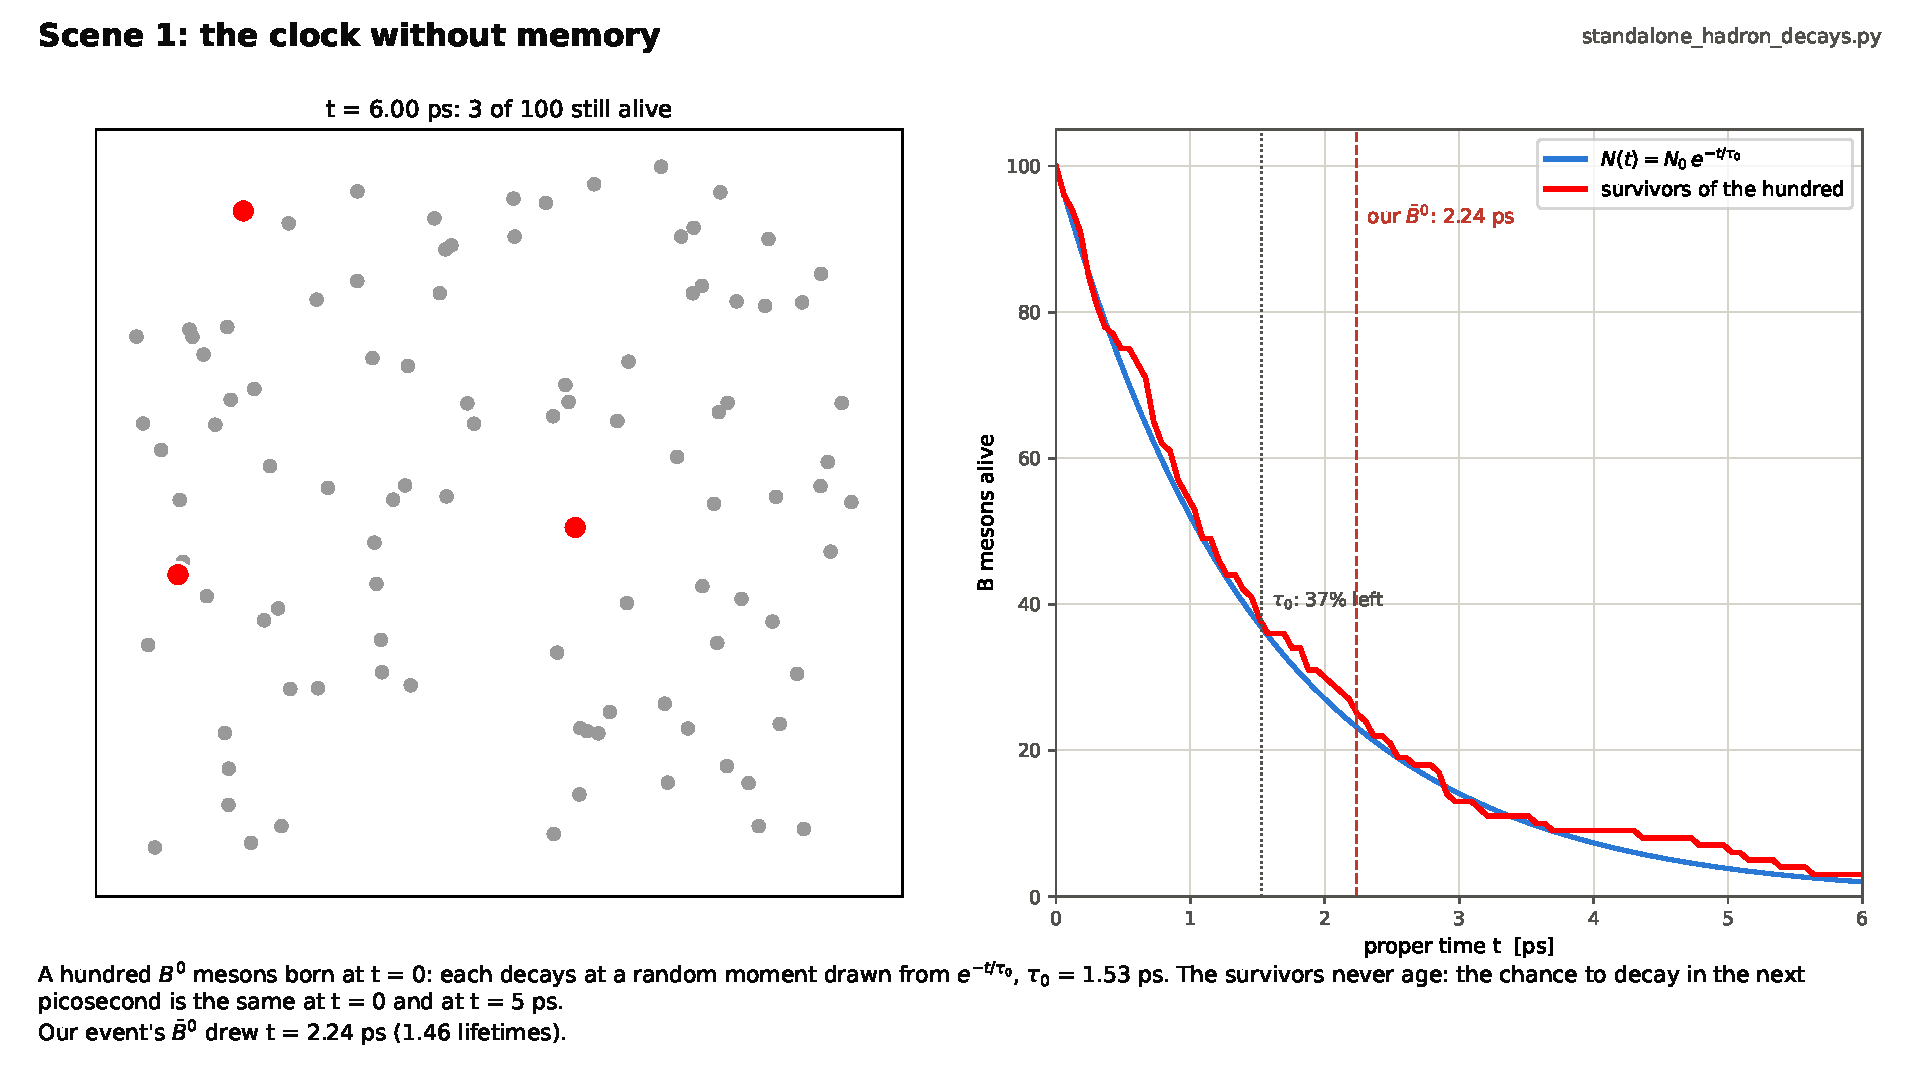
\includegraphics[page=1,width=0.325\textwidth]{Decay/Standalone/animate_standalone_hadron_decays_stills.pdf}\hfill
\includegraphics[page=2,width=0.325\textwidth]{Decay/Standalone/animate_standalone_hadron_decays_stills.pdf}\hfill
\includegraphics[page=3,width=0.325\textwidth]{Decay/Standalone/animate_standalone_hadron_decays_stills.pdf}\\[1.5mm]
\includegraphics[page=4,width=0.325\textwidth]{Decay/Standalone/animate_standalone_hadron_decays_stills.pdf}\hfill
\includegraphics[page=5,width=0.325\textwidth]{Decay/Standalone/animate_standalone_hadron_decays_stills.pdf}\hfill
\includegraphics[page=6,width=0.325\textwidth]{Decay/Standalone/animate_standalone_hadron_decays_stills.pdf}\\[1.5mm]
\includegraphics[page=7,width=0.325\textwidth]{Decay/Standalone/animate_standalone_hadron_decays_stills.pdf}
\caption[Key frames of the animated standalone hadron-decay stage]{Key
frames of the seven scenes of the animated standalone hadron-decay stage,
drawn by \file{animate_standalone_hadron_decays.py} with \code{--stills},
in reading order. A hundred $B^0$ mesons on the exponential clock; the
walk of the $b$ quark's \Bbar in the transverse plane and along the beam;
the decay table as a bar and the roll of the dice; the cascade generation
by generation; the V$-$A lepton spectrum and the neutrino of seed~4
leaving the cone; the whole event decaying in laboratory time; and four
hundred decays of the same hadrons, the flight distance and the visible
share of the cone. The film itself is the sixth on the playlist of \jitjetworld.}
\label{fig:children_producing_grandchildren:stills}
\end{figure}

\paragraph{The picture to carry: the grandchildren.}
At the wedding of
\cref{ch:children_getting_married} every quark left the house in a couple
or a triple. Most of those couples do not last. Some fall apart at once,
the $\rho$, the $K^*$, the $\omega$, the $\Delta$, the $B^*$: strong or
electromagnetic decays, at the point where they were born. A few last long
enough to walk, the B~hadrons and the charm hadrons, about a picosecond,
which the boost of a jet stretches to a centimetre, and the weak force that
ends them is the same one that lets a neutron live a quarter of an hour.
Their children have children of their own, and so on, until only the
particles that the detector will treat as stable are left
(\cref{fig:children_producing_grandchildren:family_sketch}). Three things in
the picture matter for everything that follows. The weak decays start from
a displaced point, and the tracks of the grandchildren miss the collision
point by a few hundred microns: the birthmark. The number of grandchildren
is large, sixteen from one hadron here, eleven on average, so that the
detector sees a crowd where the generator had one object. And in one decay
out of five the $W$ inside the hadron becomes a lepton and a neutrino: the
lepton walks out through the calorimeter and the neutrino emigrates, and
the jet is poorer by a tenth of its energy on average, by $40\%$ and
more in the unlucky cases. The rules are a table of branching ratios measured over
forty years~\cite{ParticleDataGroup:2024cfk,HeavyFlavorAveragingGroupHFLAV:2024ctg},
a few matrix elements, and, for half of the B~hadron's table, the string
machinery of the previous stop applied to the quarks the $W$ leaves behind.

\begin{figure}[htbp]\centering
\resizebox{\textwidth}{!}{% ---------------------------------------------------------------------------
% The grandchildren: (a) the decay tree of the mother's hadron in our event
% (the -v log, rows 1012 to 2247), generation by generation from left to
% right, with the distance each weakly decaying hadron walked before it
% decayed; (b) the emigrant: a semileptonic decay of the same hadron (seed 4
% of the ensemble) in which the neutrino leaves the cone for good and the
% muon walks out through the calorimeter.
% ---------------------------------------------------------------------------
\begin{tikzpicture}[x=1cm,y=1cm,
  every node/.style={font=\footnotesize},
  had/.style={rounded corners=2pt,draw=black!60,fill=white,inner sep=2pt,align=center,font=\scriptsize},
  bh/.style={had,draw=red!70!black,fill=red!8,font=\scriptsize\bfseries},
  ch/.style={had,draw=orange!80!black,fill=orange!12},
  fin/.style={had,draw=black!50,fill=black!5},
  gam/.style={had,draw=yellow!60!black,fill=yellow!18},
  lnk/.style={-{Stealth[length=1.6mm]},black!55,thin},
  walk/.style={-{Stealth[length=2.2mm]},red!80!black,line width=1.5pt,dashed},
  cwalk/.style={-{Stealth[length=2mm]},orange!80!black,line width=1.2pt,dashed},
  lab/.style={font=\scriptsize,align=center},
  head/.style={font=\small\bfseries}]
% ---------------- (a) the tree -----------------------------------------------------------------
\node[head,anchor=west] at (-0.8,5.1) {(a) the grandchildren of the mother's hadron: six generations, three weak decays, three vertices};
\node[bh] (B0) at (0,0) {$\bar B^{*0}$ ($b\bar d$)\\ row 1012};
\node[gam] (g1) at (2.3,1.6) {$\gamma$, $0.57\GeV$};
\node[bh] (B) at (2.3,0) {$\bar B^0$ ($b\bar d$)\\ row 1527};
\draw[lnk] (B0) -- (g1); \draw[lnk] (B0) -- (B);
\node[lab,anchor=north] at (1.15,-0.55) {strong: at the origin};
\draw[walk] (B.east) -- (5.0,0);
\node[lab,text=red!80!black,anchor=south] at (3.65,0.12) {$2.24\,\mathrm{ps}$: $L=21.0\,\mathrm{mm}$};
\node[ch] (Ds) at (6.0,2.6) {$D_s^{*-}$ ($\bar c s$)};
\node[ch] (D0s) at (6.0,0.0) {$D^{*0}$ ($c\bar u$)};
\node[had] (rho) at (6.0,-2.3) {$\rho^+$ ($u\bar d$)};
\foreach \t in {Ds,D0s,rho} {\draw[lnk] (5.0,0) -- (\t);}
\node[lab,anchor=north] at (4.2,-3.55) {$b\to cW^-$, $W^-\to s\bar c$, spectator $\bar d$ (meMode 43, BR $7.4\%$)};
\node[ch] (Dsm) at (8.5,3.2) {$D_s^-$ ($\bar c s$)}; \node[gam] (g2) at (8.5,2.1) {$\gamma$};
\node[ch] (D0) at (8.5,0.6) {$D^0$ ($c\bar u$)}; \node[gam] (g3) at (8.5,-0.5) {$\gamma$};
\node[fin] (pi1) at (8.5,-1.8) {$\pi^+$}; \node[had] (pi0a) at (8.5,-2.8) {$\pi^0$};
\draw[lnk] (Ds) -- (Dsm); \draw[lnk] (Ds) -- (g2); \draw[lnk] (D0s) -- (D0); \draw[lnk] (D0s) -- (g3);
\draw[lnk] (rho) -- (pi1); \draw[lnk] (rho) -- (pi0a);
\draw[cwalk] (Dsm.east) -- (10.7,3.2); \node[lab,text=orange!80!black,anchor=south] at (9.6,3.3) {$+5.4\,\mathrm{mm}$};
\draw[cwalk] (D0.east) -- (10.7,0.6); \node[lab,text=orange!80!black,anchor=south] at (9.6,0.7) {$+11.0\,\mathrm{mm}$};
\node[had] (Ksm) at (11.6,3.9) {$K^{*-}$ ($s\bar u$)}; \node[had] (Ks0) at (11.6,2.6) {$K^{*0}$ ($d\bar s$)};
\draw[lnk] (10.7,3.2) -- (Ksm); \draw[lnk] (10.7,3.2) -- (Ks0);
\node[fin] (Km) at (11.6,1.4) {$K^-$ ($s\bar u$)}; \node[had] (om) at (11.6,0.5) {$\omega$}; \node[fin] (pi2) at (11.6,-0.4) {$\pi^+$};
\draw[lnk] (10.7,0.6) -- (Km); \draw[lnk] (10.7,0.6) -- (om); \draw[lnk] (10.7,0.6) -- (pi2);
\node[gam] (gg1) at (11.6,-2.8) {$\gamma\gamma$};
\draw[lnk] (pi0a) -- (gg1);
\node[fin] (K0b) at (14.2,4.4) {$\bar K^0\to K_S^0$}; \node[fin] (pim1) at (14.2,3.5) {$\pi^-$};
\node[fin] (Kp) at (14.2,2.6) {$K^+$ ($u\bar s$)}; \node[fin] (pim2) at (14.2,1.7) {$\pi^-$};
\draw[lnk] (Ksm) -- (K0b); \draw[lnk] (Ksm) -- (pim1); \draw[lnk] (Ks0) -- (Kp); \draw[lnk] (Ks0) -- (pim2);
\node[fin] (pi3) at (14.2,0.9) {$\pi^+$}; \node[fin] (pim3) at (14.2,0.1) {$\pi^-$}; \node[gam] (gg2) at (14.2,-0.7) {$\pi^0\to\gamma\gamma$};
\draw[lnk] (om) -- (pi3); \draw[lnk] (om) -- (pim3); \draw[lnk] (om) -- (gg2);
\draw[decorate,decoration={brace,mirror,amplitude=4pt}] (15.6,4.8) -- (15.6,-3.5) node[midway,right=5pt,lab,text width=3.1cm,align=left] {16 final particles:\\ 8 charged ($3\pi^+$, $3\pi^-$, $K^+$, $K^-$),\\ 7 photons, one $K_S^0$;\\ no neutrino, nothing lost};
\node[lab,anchor=north west,text=black!65] at (-0.8,-4.2) {the $\rho^+$, $D^{*}$, $K^{*}$, $\omega$ and $\pi^0$ decay where they are born (strong or electromagnetic, $\tau_0=0$ on this scale); only the three weak decays, $\bar B^0$, $D_s^-$ and $D^0$, walk};
% ---------------- (b) the emigrant --------------------------------------------------------------
\begin{scope}[yshift=-7.6cm]
\node[head,anchor=west] at (-0.8,1.9) {(b) the emigrant: a neutrino leaves the family for good (seed 4)};
\fill[blue!6] (0,0) -- (7.5,1.7) -- (7.5,-1.7) -- cycle;
\draw[blue!50!black,thin] (0,0) -- (7.5,1.7); \draw[blue!50!black,thin] (0,0) -- (7.5,-1.7);
\node[lab,text=blue!50!black,anchor=west] at (7.6,-1.6) {the cone $\dR<0.4$};
\fill[red!80!black] (0,0) circle (1.3mm); \node[lab,anchor=north] at (0,-0.2) {$\bar B^0$};
\draw[walk] (0,0) -- (1.6,0.1);
\node[ch] (Dst) at (2.9,-0.9) {$D^{*-}$ ($\bar cd$)}; \draw[lnk] (1.6,0.1) -- (Dst);
\foreach \x/\y in {5.2/-1.3,5.6/-0.9,6.1/-1.5,5.0/-0.6,6.4/-0.8} {\fill[black!60] (\x,\y) circle (0.8mm); \draw[lnk] (Dst) -- (\x,\y);}
\draw[-{Stealth[length=2mm]},orange!80!black,line width=1.3pt] (1.6,0.1) -- (7.9,0.9); \node[lab,text=orange!80!black,anchor=west] at (8.0,0.9) {$\mu^+$: a track, then a hit in the muon chambers};
\draw[-{Stealth[length=2mm]},green!50!black,line width=1.3pt,dashed] (1.6,0.1) -- (9.4,2.3); \node[lab,text=green!50!black,anchor=west] at (9.5,2.3) {$\nu_\mu$: $19.8\GeV$ of energy, $12\%$ of the B, never seen: through the calorimeter and out};
\draw[black!40,line width=3pt] (7.5,-2.0) -- (7.5,1.9); \node[lab,anchor=west,text=black!55] at (7.6,-0.3) {calorimeter};
\node[lab,anchor=north west,text width=7.6cm,align=left] at (8.4,0.35) {the $\bar B^0$ oscillates and decays as $B^0\to D^{*-}\mu^+\nu_\mu$ (meMode 22, V$-$A): the muon is hard, $21.8\GeV$, the neutrino softer, and the detector will never recover it. The cone's \pt drops from $99.2$ to $89.7\GeV$ in that decay; over 400 decays of the same hadrons the visible \pt averages $91.1\pm12.2$ against $98.8\GeV$ of final particles. Our seed-1 decay is hadronic and loses nothing.};
\end{scope}
\end{tikzpicture}
}
\caption[The grandchildren: the decay tree of the mother's hadron and the
emigrant]{The grandchildren. Top: the decay tree of the mother's hadron in
our event, rows 1012 to 2247 of the record, generation by generation from
left to right: the \Bstarbar ($b\bar d$) radiates its photon at the
origin, the \Bbar ($b\bar d$) walks $21.0\mm$ and decays through
$b\to cW^-$, $W^-\to s\bar c$ into a $D_s^{*-}$ ($\bar cs$), a $D^{*0}$
($c\bar u$) and a $\rho^+$ ($u\bar d$), the two charm hadrons walk on, and
after six generations sixteen particles are left that the detector can
see. Bottom: the emigrant, seed~4 of the ensemble, in which the same
hadron oscillates and decays as $B^0\to D^{*-}\mu^+\nu_\mu$, the neutrino
leaves the cone for good and the muon walks out through the calorimeter.
Every hadron carries its quark content in brackets at its first mention,
the convention of this book.}
\label{fig:children_producing_grandchildren:family_sketch}
\end{figure}

\paragraph{The number, three ways.}
\label{sec:children_producing_grandchildren:validation}
\label{sec:children_producing_grandchildren:standalone_code}
\Cref{tab:children_producing_grandchildren:numbers} gives away the ending.
As in \cref{ch:children_getting_married} the sharpest column pair is a
comparison on identical input, this time the 365 primary hadrons of
\file{event_Had.lhe} decayed four hundred times by \PYTHIA~8.315 and by the
script. The two agree on everything the detector will see within the
statistics of four hundred decays: the multiplicities to $0.2\%$, the
flight distances, the neutrino energy, the impact parameters, the cone
momenta to $0.1\GeV$ before the neutrinos and $1\GeV$ after them. The other
columns are \PYTHIA's full chain from the hard event with decays on, our
single seed-1 decay, and the \CMSSW event.

The standalone script is a port of \PYTHIA~8's \code{ParticleDecays} class
into Python that needs NumPy and nothing else; it imports the
hadronisation script of \cref{ch:children_getting_married} for the record,
the Lorentz frames and the flavour selection, and reads its decay tables,
$161$ particles and $3114$ channels with their branching ratios,
matrix-element modes and \code{onMode} flags, from a file dumped once from
\PYTHIA's own particle data. Its learning mode, \code{-v}, prints the rule
for who decays with the lifetimes and the mixing parameters, the
composition of the tables by class, and then, for the chains of the two
B~hadrons, every decay in full: the lifetime draw with its random number,
the vertex, the mixing probability and its draw, the channel with its
branching ratio, the parton pairing and the Poisson draw, the masses, the
phase-space tries and the matrix-element weight, and the products with the
conservation check; \code{-vv} does the same for every decay. The $3200$
lines of \code{-v} for seed~1 are committed, and every number quoted in
the theory of this chapter is taken from that log.
\label{sec:children_producing_grandchildren:pythia}

The first official check is again on identical input: \PYTHIA with its
process level switched off, its record filled by hand with the $365$
primary hadrons of \file{event_Had.lhe}, decaying them four hundred times
with \code{ParticleDecays:limitTau0 = on} and \code{tau0Max = 10}, and a
$B^0$ at rest twenty thousand times, which removes the boost and the rest
of the event and tests the tables, the matrix elements and the mixing
alone. Read the first two columns of the table together. \PYTHIA makes
$739.2\pm11.9$ final particles from our hadrons where the script makes
$740.3\pm11.7$, $331.1$ against $331.2$ charged, $328.8$ against $330.0$
photons, and the species agree to a tenth of a percent of the final state.
For the mother's hadron the two agree on the flight distance, $13.2$
against $14.5\mm$ with a width of $13$, on the number of its final
particles, $11.05$ against $11.08$, on its neutrino energy, on the impact
parameters of its tracks, on the final \pt of the cone to $0.01\GeV$ and
on the visible \pt to $1.2\GeV$ with a width of $12$. The $B^0$ at rest
resolves two small differences: the script makes $2\%$ more particles,
almost all of them photons from the $\pi^0$ of its partonic channels, and
it splits the charm hadrons differently, $30\%$ $D^-$ and $28\%$
$\bar D^0$ where \PYTHIA has $35$ and $27$, the spectator deviation of
\cref{sec:children_producing_grandchildren:caveats}; the semileptonic fraction,
$20.51$ against $20.70\%$, and the lepton spectrum, $1.396$ against
$1.383\GeV$, agree, and so does the oscillated fraction of
\cref{sec:children_producing_grandchildren:mixing}, $16.5$ against
$16.8\%$. The full chain, with the B~hadron species mixed and
the hadrons harder, gives the same semileptonic fractions and neutrino
shares as the same-hadron columns and a wider everything else.
\label{sec:children_producing_grandchildren:cmssw}

The second official check is the \code{GEN} step of
\cref{sec:ancestral_home:cmssw} with its last switch turned on, the hadron
decays; in production \code{HadronLevel:all} covers them, and
\code{ParticleDecays:limitTau0 = on} with \code{tau0Max = 10} is in every
CMS configuration. This job decayed its $b$ and $c$ hadrons with \PYTHIA's
own tables, the ones the script embeds; the production configurations of
CMS hand them to EvtGen~\cite{Lange:2001uf} through the external-decayer
interface instead, with PHOTOS for the radiative corrections and TAUOLA for
the $\tau$, and \cref{sec:children_producing_grandchildren:caveats} says what changes. Its event is the
last column of the table, and \cref{sec:children_producing_grandchildren:our_jet_at_this_stage} follows
the mother through its record. How each column was produced, the commands,
the modes and the logs, is in the companion of this chapter,
\begin{center}
  \companion{chapter_06_Decay}
\end{center}
together with the full tables behind every number quoted below.

\begin{table}[htbp]\centering\small
\caption[Hadron decays obtained three ways]{Hadron decays obtained three
ways. ``Same hadrons'' means the 365 primary hadrons of
\file{example/Had/event_Had.lhe}, decayed $400$ times by \PYTHIA~8.315 with
\code{ParticleDecays:limitTau0 = on} and by the standalone script; ``full
chain'' means \PYTHIA from the hard event of \cref{ch:ancestral_home} with
the CP5 settings and decays on, $2000$ events with the impact parameter
drawn. The spread of a single event follows $\pm$. ``The B'' is the weakly
decaying hadron of the $b$ quark, \Bbar ($b\bar d$) in every same-hadron
column; in the full chain it is a $B^-$ ($b\bar u$) in $44\%$ of the
events, a \Bbar in $43$, a $\bar B_s^0$ ($b\bar s$) in $10$ and a
$\Lambda_b^0$ ($udb$) in $4$. ``Visible'' excludes the neutrinos. The
\CMSSW column is the single event of \cref{ch:ancestral_home} with the
decays on; its $B^-$ decayed semileptonically.}
\label{tab:children_producing_grandchildren:numbers}
\scriptsize\setlength{\tabcolsep}{3pt}
\resizebox{\textwidth}{!}{%
\begin{tabular}{lrrrrr}\toprule
 & \PYTHIA & standalone & \PYTHIA full & standalone & \CMSSW \\
 & same hadrons & same hadrons & $b$ drawn & seed 1 & 1 event \\ \midrule
final particles & $739\pm12$ & $740\pm12$ & $459\pm175$ & $749$ & $634$ \\
\quad charged / photons / neutrinos & $331$ / $329$ / $2.9$ & $331$ / $330$ / $3.1$ & $210$ / $211$ / $1.3$ & $338$ / $327$ / $5$ & $304$ / $273$ / $1$ \\
\quad decays performed & $371$ & $372$ & $221$ & $376$ & $302$ \\
\quad primary hadrons that survive & $143$ & $143$ & $86$ & $143$ & $132$ \\ \midrule
the B: $\tau$ [ps] & $1.41\pm1.40$ & $1.55\pm1.46$ & $1.59\pm1.60$ & $2.24$ & -- \\
the B: $L$, \Lxy [mm] & $13.2$, $6.2$ & $14.5$, $6.8$ & $18.7$, $7.9$ & $21.0$, $9.9$ & $7.83$, $3.13$ \\
the B: final particles (charged) & $11.1$ ($5.0$) & $11.1$ ($4.9$) & $11.0$ ($4.8$) & $15$ ($8$) & $9$ ($3$) \\
the B: semileptonic $e$ / $\mu$ / $\tau$ [\%] & $9.5$ / $10.0$ / $4.0$ & $13.0$ / $11.0$ / $1.2$ & $10.9$ / $11.4$ / $3.4$ & hadronic & $e$ \\
the B: $E_\nu$ [GeV], share of $E_B$ & $13.8$, $0.084$ & $16.4$, $0.099$ & $18.6$, $0.091$ & $0$, $0$ & $95.5$, $0.40$ \\
the B: tracks with $|\dzero|>100\um$, mean $|\dzero|$ [$\mu$m] & $3.0$, $330$ & $3.0$, $362$ & $3.0$, $358$ & $8$, max $1640$ & -- \\
the B: oscillated [\%] & $16.5$ & $16.8$ & $12.3$ & no & no \\ \midrule
$b$, $\dR<0.4$: primaries $\to$ final $\to$ visible \pt [GeV] & $99.23\to98.79\to92.3\pm11.4$ & $99.23\to98.79\to91.1\pm12.2$ & $109.2\to109.3\to101.4$ & $99.23\to99.43\to99.43$ & $114.45\to\;\cdot\;\to79.12$ \\
$b$, $\dR<0.4$: final particles (charged) & $24.6$ ($9.6$) & $24.7$ ($9.5$) & $21.0$ ($9.2$) & $31$ ($16$) & -- \\
$b$, $\dR<0.4$: charged \pt [GeV], B share & $51.3$, $0.788$ & $49.9$, $0.788$ & $60.6$, $0.799$ & $67.4$, $0.79$ & -- \\
$b$, $\dR<0.4$: mass, primaries $\to$ final [GeV] & $16.1\to14.1$ & $16.1\to14.2$ & $14.2\to12.3$ & $16.1\to14.6$ & -- \\
$b$, $\dR<0.8$: final $\to$ visible \pt [GeV] & $107.2\to100.7$ & $107.2\to99.5$ & $119.2\to111.3$ & $108.73\to108.73$ & -- \\ \midrule
$\bar b$: $L$, \Lxy [mm] & $119$, $7.7$ & $117$, $7.6$ & $152$, $7.4$ & $146.9$, $9.5$ & $117.3$, $5.5$ \\
$\bar b$, $\dR<0.4$: final $\to$ visible \pt [GeV] & $92.4\to85.7\pm11.3$ & $92.4\to84.7\pm12.7$ & $106.3\to99.1$ & $92.99\to92.99$ & $115.94\to115.94$ \\ \midrule
$B^0$ at rest ($20\,000$): final / charged / photons & $10.87$ / $4.85$ / $4.50$ & $11.11$ / $4.90$ / $4.77$ & -- & -- & -- \\
$B^0$ at rest: semileptonic ($e+\mu$) [\%], $\langle E_\ell\rangle$ [GeV] & $20.7$, $1.383$ & $20.5$, $1.396$ & -- & -- & -- \\
$B^0$ at rest: $D^-$ / $\bar D^0$ / $D^0$ / $D^+$ [\%] & $35$ / $27$ / $11$ / $10$ & $30$ / $28$ / $12$ / $9$ & -- & -- & -- \\
\bottomrule
\end{tabular}}
\end{table}

\section{Let us dive into the details: the theory}
\label{sec:children_producing_grandchildren:theory}

\subsection{B-hadron lifetimes and displaced vertices: the family's birthmark}
\label{sec:children_producing_grandchildren:b_hadron_lifetimes_and_displaced_vertice}

Before the grandchildren, the walk: how long a hadron lives, how far that
takes it, and what of the walk is left for the detector to find.

\subsubsection{The clock without memory: the decay law and the 10 mm rule}
\label{sec:children_producing_grandchildren:lifetime}

Guess first. Of the 365 primary hadrons of the record, which ones should
the generator decay, and which should it leave alone? Every one of them
decays eventually, even the proton is only known to live longer than the
universe, but a $\pi^+$ ($u\bar d$) at $10\GeV$ flies $560\,\mathrm{m}$
before it does, through the whole of CMS, and a $K_S^0$ ($d\bar s$ and
$s\bar d$, the short-lived mixture) at $10\GeV$ flies half a metre, into
the tracker, where its two pions are seen as a V. The generator cannot
know the detector's geometry, so \PYTHIA draws a line in proper flight
length: a particle decays in the generator if its decay table is open and
its $c\tauz$ is below \code{ParticleDecays:tau0Max}, which CMS sets to
$10\mm$ (\code{limitTau0 = on}; \PYTHIA's own default is to decay
everything with a table, which the script reproduces with
\code{--no-limit-tau0}). Everything above the line, the $K_S^0$ at
$26.8\mm$, the $\Lambda$ ($uds$) at $78.9$, the $\Sigma$, $\Xi$ and
$\Omega^-$ ($sss$) hyperons, the charged pions and kaons, the $K_L^0$, the
neutron and the muon, is handed to GEANT4~\cite{GEANT4:2002zbu} in
\cref{ch:crossing_the_border}, which knows where the material is. Below
the line are the $\pi^0$ ($25\,\mathrm{nm}$), the $\eta$ and $\eta'$, the
resonances with no measurable lifetime at all, the $\tau$ lepton
($87\um$), the charm hadrons ($21$ to $312\um$) and the bottom hadrons
($138$ to $491\um$). The scale of the line is what matters: a B~hadron's
$c\tauz$ is half a millimetre, and that half millimetre is what this
section is about.

\begin{figure}[htbp]\centering
\resizebox{\textwidth}{!}{% ---------------------------------------------------------------------------
% Lifetimes. (a) The decay law: the survivors of a population follow
% exp(-t/tau0) and the clock has no memory; the proper times drawn for the
% two B hadrons of our event are marked. (b) The walk in the laboratory,
% L = gamma beta c tau: the b quark's B at gamma beta = 31 and the bbar's at
% 239, to the same proper-time scale. (c) The ladder of c tau0 with the
% generator's 10 mm line: who decays in PYTHIA and who in the detector.
% ---------------------------------------------------------------------------
\begin{tikzpicture}[x=1cm,y=1cm,
  every node/.style={font=\footnotesize},
  lab/.style={font=\scriptsize,align=center},
  head/.style={font=\small\bfseries},
  walk/.style={-{Stealth[length=2.2mm]},line width=1.6pt}]
% ---------------- (a) the decay law --------------------------------------------------------------
\begin{scope}
\node[head,anchor=west] at (-0.4,4.75) {(a) the clock without memory};
\draw[-{Stealth}] (0,0) -- (5.6,0) node[below left,lab] {$t/\tau_0$};
\draw[-{Stealth}] (0,0) -- (0,4.3) node[left,lab] {$N(t)/N_0$};
\foreach \x in {1,2,3,4,5} {\draw (\x,-0.06) -- (\x,0.06); \node[lab,anchor=north] at (\x,-0.08) {\x};}
\foreach \y/\t in {1/0.25,2/0.5,3/0.75,4/1} {\draw (-0.06,\y) -- (0.06,\y); \node[lab,anchor=east] at (-0.08,\y) {\t};}
\draw[blue!70!black,thick] plot[domain=0:5.5,samples=60] (\x,{4*exp(-\x)});
\node[lab,text=blue!70!black,anchor=west] at (2.3,2.4) {$N(t)=N_0\,e^{-t/\tau_0}$};
\draw[dashed,black!60] (1,0) -- (1,{4*exp(-1)}) -- (0,{4*exp(-1)});
\node[lab,anchor=west] at (1.05,1.75) {$\tau_0$: $37\%$ left};
\draw[red!80!black,thick] (1.46,0) -- (1.46,{4*exp(-1.46)}); \fill[red!80!black] (1.46,{4*exp(-1.46)}) circle (1mm);
\node[lab,text=red!80!black,anchor=west] at (1.6,1.15) {the $b$'s $\bar B^0$: $t=1.46\,\tau_0=2.24\,\mathrm{ps}$\\ ($r=0.768$, $23\%$ would still be alive)};
\draw[blue!80!black,thick] (1.34,0) -- (1.34,{4*exp(-1.34)}); \fill[blue!80!black] (1.34,{4*exp(-1.34)}) circle (1mm);
\node[lab,text=blue!80!black,anchor=west] at (2.3,0.55) {the $\bar b$'s $B^0$: $1.34\,\tau_0=2.05\,\mathrm{ps}$};
\node[lab,anchor=north west,text width=5.6cm,align=left,text=black!65] at (-0.4,-0.55) {the chance to decay in the next picosecond is the same at $t=0$ and at $t=5\,\mathrm{ps}$; a draw $t=-\tau_0\ln(1-r)$ reproduces the curve, $\tau_0=1.530\,\mathrm{ps}=0.459\,\mathrm{mm}/c$ for a $B^0$};
\end{scope}
% ---------------- (b) the walk ------------------------------------------------------------------
\begin{scope}[xshift=7.0cm]
\node[head,anchor=west] at (-0.4,4.75) {(b) the walk: $L=\gamma\beta\,c\tau$};
\fill[black!70] (0,3.2) circle (1.2mm); \node[lab,anchor=east] at (-0.15,3.2) {primary\\ vertex};
\draw[walk,red!80!black] (0,3.2) -- (2.1,3.2); \fill[red!80!black] (2.1,3.2) circle (1mm);
\node[lab,text=red!80!black,anchor=south west] at (0,3.3) {$\bar B^0$ of the $b$: $\gamma\beta=31.3$, $9.4\,\mathrm{mm}$ per ps};
\node[lab,text=red!80!black,anchor=north west] at (0,3.05) {$2.24\,\mathrm{ps}\to L=21.0\,\mathrm{mm}$ ($L_{xy}=9.9$)};
\fill[black!70] (0,1.3) circle (1.2mm);
\draw[walk,blue!80!black] (0,1.3) -- (5.0,1.3); \draw[blue!80!black,line width=1.6pt] (5.2,1.2) -- (5.4,1.4) (5.5,1.2) -- (5.7,1.4); \draw[walk,blue!80!black] (5.9,1.3) -- (6.6,1.3); \fill[blue!80!black] (6.6,1.3) circle (1mm);
\node[lab,text=blue!80!black,anchor=south west] at (0,1.4) {$B^0$ of the $\bar b$ ($\eta=-3.4$): $\gamma\beta=239$, $72\,\mathrm{mm}$ per ps};
\node[lab,text=blue!80!black,anchor=north west] at (0,1.15) {$2.05\,\mathrm{ps}\to L=146.9\,\mathrm{mm}$, almost all along the beam ($L_{xy}=9.5$)};
\draw[black!40] (0,-0.2) -- (2.1,-0.2); \node[lab,anchor=west,text=black!65] at (2.2,-0.2) {$=21\,\mathrm{mm}$ (the scale of the two arrows)};
\node[lab,anchor=north west,text width=6.4cm,align=left,text=black!65] at (-0.4,-0.55) {the same proper time, a different walk: the boost stretches the clock. The \CMSSW $B^-$ walked $7.83\,\mathrm{mm}$; over 400 decays the $b$'s hadron walks $14.5\pm13.6\,\mathrm{mm}$, $6.8$ in the transverse plane};
\end{scope}
% ---------------- (c) the ladder ------------------------------------------------------------------
\begin{scope}[xshift=15.8cm]
\node[head,anchor=west] at (-0.4,4.75) {(c) who decays where: $c\tau_0$};
% log10(c tau0 / mm) from -5 to 15 mapped to y = 0 .. 4.2 => y = (lg + 5) * 0.21
\draw[-{Stealth}] (0,-0.1) -- (0,4.45) node[left,lab] {$c\tau_0$};
\foreach \lgv/\t in {-4/{$0.1\,\mu$m},-2/{$10\,\mu$m},0/{$1$ mm},2/{$10$ cm},4/{$10$ m},6/{$1$ km},14/{$10^{11}$ m}} {\draw (-0.06,{(\lgv+5)*0.21}) -- (0.06,{(\lgv+5)*0.21}); \node[lab,anchor=east] at (-0.08,{(\lgv+5)*0.21}) {\t};}
\draw[red!80!black,thick,dashed] (-0.2,{(1+5)*0.21}) -- (6.2,{(1+5)*0.21}); \node[lab,text=red!80!black,anchor=west,text width=2.4cm,align=left] at (6.3,{(1+5)*0.21}) {$\tau_0^{\max}=10\,\mathrm{mm}$: above it the detector decays them (GEANT4)};
\foreach \lgv/\x/\t in {-4.6/0.6/{$\pi^0$}, -1.06/1.0/{$\tau$}, -1.22/1.4/{$\Lambda_c^+$}, -0.91/1.8/{$D^0$}, -0.82/2.2/{$D_s^+$}, -0.51/2.6/{$D^+$}, -0.36/3.0/{$B_s^0$}, -0.36/3.4/{$\Lambda_b^0$}, -0.34/3.8/{$B^0$}, -0.31/4.2/{$B^+$}} {
  \fill[red!75!black] (\x-0.12,0) rectangle (\x+0.12,{(\lgv+5)*0.21}); \node[lab,anchor=west,rotate=90,text=red!75!black] at (\x,{(\lgv+5)*0.21+0.03}) {\t};}
\foreach \lgv/\x/\t in {1.43/0.6/{$K_S^0$}, 1.38/1.0/{$\Sigma^+$}, 1.69/1.4/{$\Xi^-$}, 1.90/1.8/{$\Lambda$}, 3.57/2.2/{$K^+$}, 3.89/2.6/{$\pi^+$}, 4.18/3.0/{$K_L^0$}, 5.82/3.4/{$\mu$}, 14.4/3.8/{$n$}} {
  \fill[black!45] (\x-0.12,{(1+5)*0.21}) rectangle (\x+0.12,{(\lgv+5)*0.21}); \node[lab,anchor=west,rotate=90,text=black!65] at (\x,{(\lgv+5)*0.21+0.03}) {\t};}
\node[lab,anchor=north west,text width=5.8cm,align=left,text=black!65] at (-0.4,-0.55) {red: decayed by the generator, $c\tau_0$ of $25\,$nm ($\pi^0$) to $0.49\,$mm ($B^+$); grey: handed to the detector. The $\rho$, $K^*$, $\omega$, $\Delta$, $B^*$ and $D^*$ have no bar at all, they decay where they are born};
\end{scope}
\end{tikzpicture}
}
\caption[The decay law, the walk and the ladder of lifetimes]{Lifetimes.
Left: the decay law, \cref{eq:children_producing_grandchildren:decay_law},
and the proper times drawn for the two B~hadrons of our event. Middle: the
walk, \cref{eq:children_producing_grandchildren:flight}, for the $b$
quark's \Bbar at $\gamma\beta=31$ and the $\bar b$'s $B^0$ ($d\bar b$) at
$239$, to the same proper-time scale. Right: the ladder of $c\tauz$ with
the generator's $10\mm$ line: red decays in \PYTHIA, grey in the detector.}
\label{fig:children_producing_grandchildren:clock_sketch}
\end{figure}

An unstable particle has no age. Its probability to decay in the next
instant is a constant, $\Gamma=1/\tauz$, whatever happened before, and the
population of a hundred B~mesons born together therefore falls as
\begin{equation}
  N(t)=N_0\,e^{-t/\tauz},\qquad
  P(t)\,\mathrm{d}t=\frac{1}{\tauz}e^{-t/\tauz}\,\mathrm{d}t,\qquad
    t=-\tauz\ln(1-r),
  \label{eq:children_producing_grandchildren:decay_law}
\end{equation}
with $t$ the proper time, measured by a clock that travels with the
particle, and $r$ a uniform random number, the fraction of the population
that has decayed before $t$: the inverse of the cumulative distribution, the same trick as the Sudakov veto of
\cref{ch:mother_gives_birth} with a constant rate instead of a running
one. In the generator's units $c\tauz$ is a length, $1\ps=0.2998\mm/c$,
and the $B^0$'s $1.530\ps$ is $0.4587\mm$. Why that long? The weak decay of
a free $b$ quark, $b\to cW^-$ with the $W$ off shell, has the width of the
muon with the muon's mass replaced and the CKM element inserted,
\begin{equation}
  \Gamma_b\simeq N_{\mathrm{eff}}\,\frac{G_F^2\,m_b^5}{192\pi^3}\,|V_{cb}|^2\,f\!\left(\frac{m_c^2}{m_b^2}\right),
  \label{eq:children_producing_grandchildren:spectator}
\end{equation}
the \emph{spectator model}, in which the light antiquark only watches.
One channel of the $W$ at $m_b=4.8\GeV$ and $|V_{cb}|=0.041$ gives a
lifetime of $6.7\ps$; the $W$ has nine doors, three leptons and two quark
pairs in three colours each, and the phase-space factor $f$ for the charm
mass is about one half, so that $\tau_b\approx6.7/(9\times0.5)=1.5\ps$.
The two numbers that make the B~hadron live a thousand times longer than
a $\tau$ lepton would at the same mass are in the formula: $|V_{cb}|^2$,
a suppression of $600$, because the $b$ can only decay into a quark of
another generation, and the phase-space factor $f$, a further factor of
two, because that quark is heavy. The spectator picture is the leading term of an expansion in
$\Lambda_{\mathrm{QCD}}/m_b$, the heavy-quark expansion of
\cite{Bigi:1992su,Manohar:1993qn,Neubert:1993mb}, whose next terms split
the lifetimes of the $B^+$, $B^0$, $B_s^0$ and $\Lambda_b^0$ by a few
percent~\cite{Neubert:1996we,Lenz:2014jha,Lenz:2022rbq}, as the tables
record and LHCb measures~\cite{LHCb:2014qsd}. The charm hadrons spread
much more, $0.41\ps$ for the $D^0$ ($c\bar u$) against $1.04$ for the
$D^+$ ($c\bar d$), because for them the spectator is not a spectator at
all.

The walk follows from the clock. A particle of momentum $p$ and mass $m$
moves at $\beta$ and its clock runs slow by $\gamma$, so that a proper
time $\tau$ takes it a laboratory distance
\begin{equation}
  L=\gamma\beta\,c\tau=\frac{p}{m}\,c\tau,\qquad
  \vec x_{\mathrm{decay}}=\vec x_{\mathrm{prod}}+\frac{\vec p}{m}\,c\tau,\qquad
  \Lxy=\frac{\pt}{m}\,c\tau,
  \label{eq:children_producing_grandchildren:flight}
\end{equation}
with \Lxy its projection on the transverse plane, the one the tracker
measures best. The boost of a jet is large: a B~hadron of $165\GeV$ has
$\gamma\beta=31$ and walks $9.4\mm$ per picosecond of its own time.

\paragraph{The numbers.} The \code{-v} log opens with the rule and its
consequences: of the 365 primary hadrons $222$ have an open table and
$c\tauz<10\mm$, and $143$ are the detector's, $43$ $\pi^+$, $37$ $\pi^-$,
$13$ $K^+$ ($u\bar s$), $10$ $K^-$, $10$ $\bar n$, $9$ $n$, $8$ $p$, $4$
$\Sigma^+$ ($uus$), $3$ $\bar\Lambda$, $3$ $\bar p$ and $3$ $\bar\Sigma^-$.
The mother's hadron goes first through a decay that does not walk: the
\Bstarbar is a vector meson $45\,\mathrm{MeV}$ above the \Bbar and
radiates a photon at the origin, with only one channel in its table. Then
the \Bbar, row 1527, $E=165.47\GeV$, $m=5.2796$: $c\tauz=0.4587\mm$, the
random number $r=0.7682$, and \cref{eq:children_producing_grandchildren:decay_law}
gives $\tau=0.6707\mm/c=2.237\ps$, $1.46$ lifetimes, a draw that $23\%$ of
B~mesons outlive. With $\gamma\beta=p/m=31.33$ the walk of
\cref{eq:children_producing_grandchildren:flight} is $L=21.009\mm$,
$\Lxy=9.941$, and the decay vertex is $(-9.130,-3.934,-18.508)\mm$ at
$t=21.02\mm/c$ after the collision. The $\bar b$'s $B^0$, row 1590, drew
$r=0.7374$, $\tau=2.046\ps=1.34\,\tauz$, a shorter life, but at $\eta=-3.4$
its $\gamma\beta=239$ stretches it to $L=146.9\mm$, almost all along the
beam, with $\Lxy=9.52$, nearly the same as the mother's. Further down the
chain the $D^0$ of our event drew $r=0.9435$, $2.87$ lifetimes, and walked
another $10.98\mm$; the $D_s^-$ ($\bar cs$) drew $1.24$ lifetimes and
$5.44\mm$. Elsewhere in the event a $D^-$ from the shower's charm walked
$54.9\mm$, the third B~hadron of the record, a \Bbar of $360\GeV$ from the
$g\to b\bar b$ splitting of \cref{ch:mother_gives_birth}, $64.4\mm$, and
its partner $\bar\Lambda_b^0$ ($\bar u\bar d\bar b$) $14.1\mm$. Over four
hundred decays the mother's hadron lives $1.55\pm1.46\ps$, the mean of
\cref{eq:children_producing_grandchildren:decay_law} with its own width,
and walks $14.5\pm13.6\mm$, $6.8$ in the transverse plane; \PYTHIA on the
same hadron gives $1.41\ps$ and $13.2\mm$, the full chain, whose B~hadrons
are harder, $18.7\mm$; the \CMSSW $B^-$ walked $7.83\mm$. Page~1 of
\file{theory_hadron_decays.pdf}
(\cref{fig:children_producing_grandchildren:lifetime_plot}) shows the
three: the clock, the walk and the ladder.

\begin{figure}[htbp]\centering
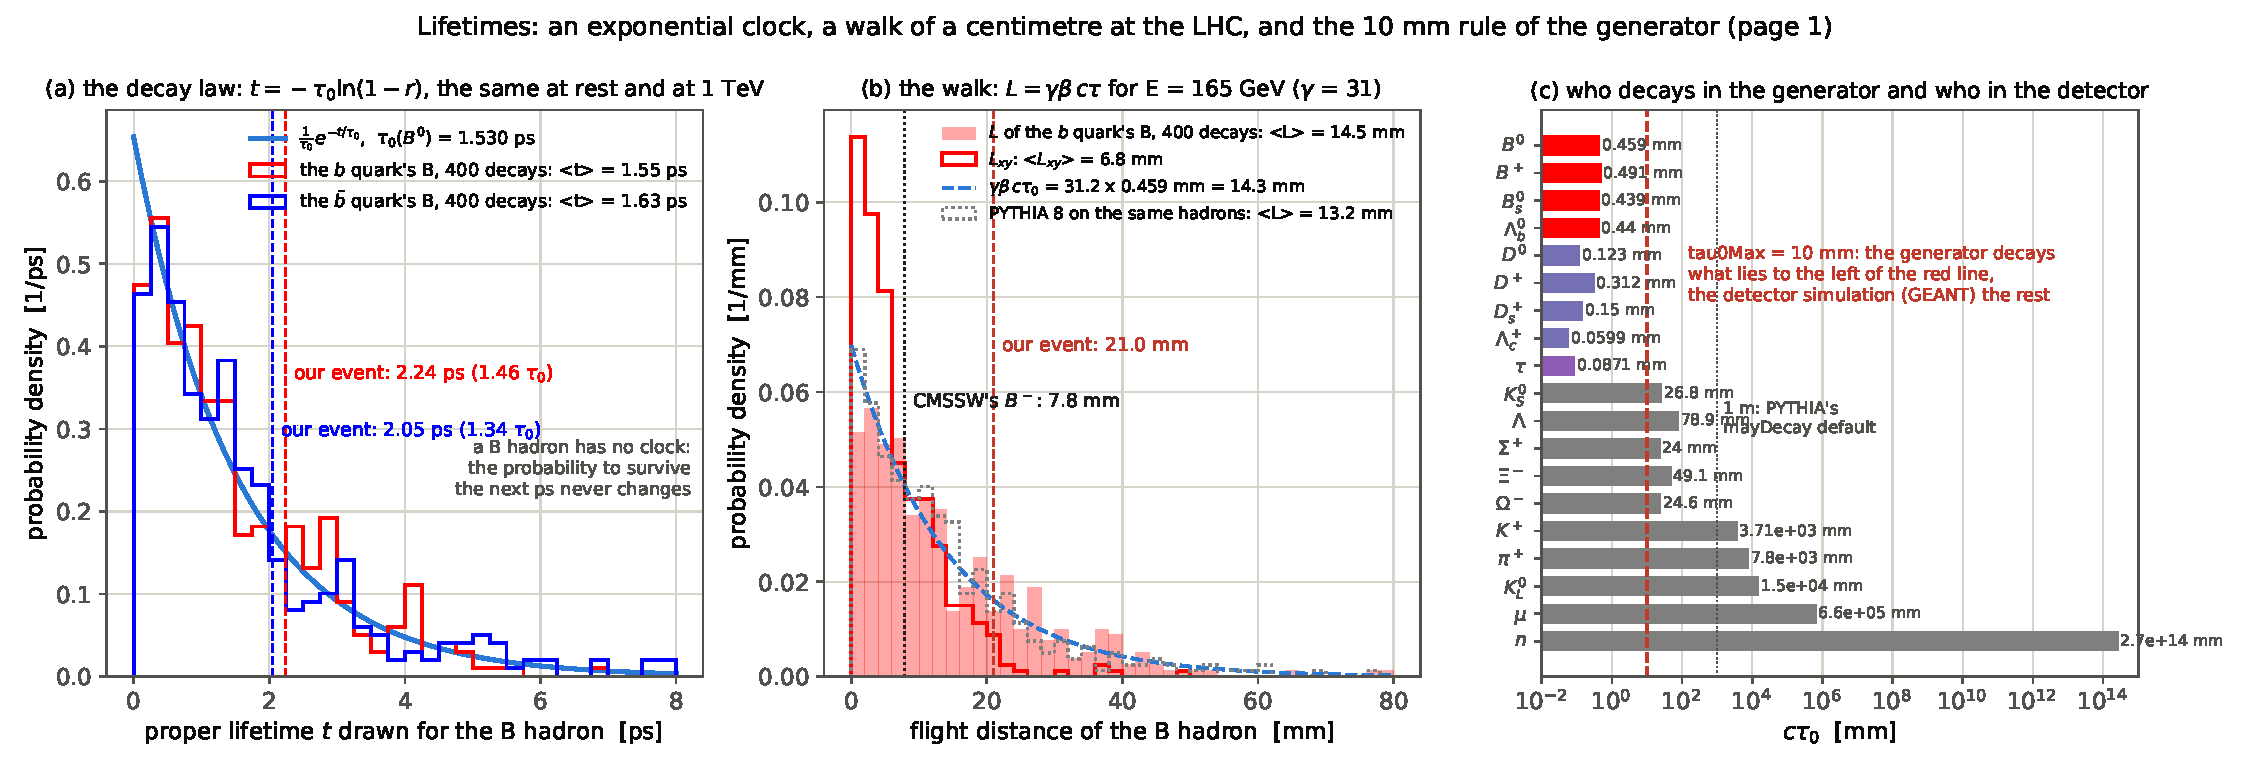
\includegraphics[page=1,width=\textwidth]{Decay/Standalone/theory_hadron_decays.pdf}
\caption[The decay law, the flight distance and the ladder of $c\tau_0$]{Page~1
of \file{theory_hadron_decays.pdf}. (a) The proper lifetimes drawn for
the two B~hadrons over 400 decays against the exponential of
\cref{eq:children_producing_grandchildren:decay_law}, with our event's
draws marked. (b) The flight distance of the $b$ quark's \Bbar,
\cref{eq:children_producing_grandchildren:flight}, for the script and
\PYTHIA on the same hadron and for the full chain, with our event and the
\CMSSW $B^-$. (c) The ladder of $c\tauz$ of the hadrons of the record with
the generator's $10\mm$ line.}
\label{fig:children_producing_grandchildren:lifetime_plot}
\end{figure}

\subsubsection{The birthmark: the decay vertex and the impact parameter}
\label{sec:children_producing_grandchildren:vertices}

Guess first: the \Bbar walked $21\mm$. What of that walk does the detector
see? Nothing of the walk itself. The \Bbar is neutral, and even a charged
B~hadron leaves at most a few hits in the first pixel layer before it is
gone; the tracker never sees the B. What it sees are the tracks of the
charged grandchildren, which start from the decay vertex and not from the
collision point, and the signature is geometric
(\cref{fig:children_producing_grandchildren:vertex_sketch}): extrapolate
any of those tracks back towards the beam and it misses the primary vertex
by a distance
\begin{equation}
  \dzero=\frac{|x_v\,p_y-y_v\,p_x|}{\pt}=\Lxy\,\sin\theta,
  \label{eq:children_producing_grandchildren:d0}
\end{equation}
the \emph{transverse impact parameter}, where $(x_v,y_v)$ is the vertex
the track starts from and $\theta$ the angle in the transverse plane
between the track and the direction of the B. The second form says
something a newcomer does not expect: \dzero does not grow with the jet's
energy. A harder B walks further, $\Lxy\propto\gamma\beta$, but its
decay products are thrown forward into a cone whose opening angle shrinks
by the same factor, $\theta\propto1/\gamma\beta$, and the product stays of
the order of $c\tauz$, a few hundred microns, at any \pt.
\Cref{fig:children_producing_grandchildren:boost_sketch} draws the
cancellation: three B~hadrons with the same proper time and the boosts
$\gamma\beta$, $3\gamma\beta$ and $9\gamma\beta$ decay along the same
axis, each walk is three times the last, each cone three times narrower,
and the back-extrapolation of every track is tangent to the same circle
of radius \dzero around the primary vertex. Written out, with
$L=\beta\gamma c\tau$ for a decay at the proper time $\tau$ and
$\sin\theta\simeq p^*_\perp/p_\parallel$ for a product whose rest-frame momentum has the
components $p^*_\perp$ and $p^*_\parallel$ and the energy $E^*$,
\begin{equation}
  \dzero=L\sin\theta
  \simeq\beta\gamma c\tau\,\frac{p^*_\perp}{\gamma\,(\beta E^*+p^*_\parallel)}
  \;\xrightarrow{\;\beta\to1\;}\;
  c\tau\,\frac{p^*_\perp}{E^*+p^*_\parallel},
  \label{eq:children_producing_grandchildren:d0boost}
\end{equation}
every $\gamma$ has cancelled, and what remains is the proper time and the
kinematics of the decay in the rest frame, the same for a B of $20\GeV$
and one of $2\TeV$. For a product of $1\GeV$ at right angles in the rest
frame it is $c\tau$ itself, and the ensemble's median of $166\um$ and
mean of $362\um$ below are that number folded with the decay kinematics.
That is why the B~hadron is found by a tracker with a resolution of tens
of microns and not by a calorimeter, and why the $b$ tag of
\cref{ch:footprints} works from $20\GeV$ to a TeV: the birthmark is the
same size on every child. Where the argument ends is the detector and
not the geometry. The walk itself does grow, $1.7\mm$ at $20\GeV$, $17$
at $200$ and $87$ at a TeV on average, so past half a TeV most B~hadrons
decay beyond the first pixel layer, a few centimetres from the beam, and
the tracks of a cone a milliradian wide begin to share pixel hits; the
tag loses its inner hits there, not its birthmark. The weak charm decay
that follows adds a third vertex a few millimetres further on, and the
tracks from it carry impact parameters of their own.

\begin{figure}[htbp]\centering
\resizebox{\textwidth}{!}{% ---------------------------------------------------------------------------
% Why the b tag works from 20 GeV to a TeV. (a) Three B hadrons of the same
% proper time and the boosts gamma*beta, 3 gamma*beta and 9 gamma*beta decay
% along the same axis: the walk L grows by three at each step, the opening
% angle theta of the decay cone shrinks by three, and the back-extrapolation
% of every track is tangent to the same circle of radius d0 around the
% primary vertex (the geometry is exact for the drawn L: sin theta = d0/L).
% (b) The same statement against pT on log scales: L_xy rises as gamma*beta,
% theta falls as 1/(gamma*beta), d0 = L sin(theta) stays a few hundred
% microns; where the walk passes the first pixel layer the tag starts to lose
% hits, which is the detector's limit and not the birthmark's.
% ---------------------------------------------------------------------------
\begin{tikzpicture}[x=1cm,y=1cm,
  every node/.style={font=\footnotesize},
  lab/.style={font=\scriptsize,align=center},
  head/.style={font=\small\bfseries},
  trk/.style={red!75!black,thick},
  walk/.style={red!80!black,line width=1.2pt,dashed}]
% ---------------- (a) the same circle at every boost ----------------------------------------------
\begin{scope}
\node[head,anchor=west] at (-1.4,2.0) {(a) three boosts, one birthmark: every track is tangent to the same circle};
\pgfmathsetmacro{\dz}{0.5}
\draw[black!40,-{Stealth}] (-1.2,0) -- (15.4,0) node[below left,lab,text=black!60] {direction of the B};
\foreach \L/\gb/\th/\colr in {1.4/{$\gamma\beta$}/{$\theta$}/red!80!black, 4.2/{$3\gamma\beta$}/{$\theta/3$}/red!60!black, 12.6/{$9\gamma\beta$}/{$\theta/9$}/red!40!black} {
  \pgfmathsetmacro{\ang}{asin(\dz/\L)}
  \pgfmathsetmacro{\back}{\L*cos(\ang)+1.0}
  % the decay cone (half-angle 1.4 theta) and the walk
  \fill[\colr,opacity=0.10] (\L,0) -- ++({1.4*\ang}:2.2) arc ({1.4*\ang}:{-1.4*\ang}:2.2) -- cycle;
  \draw[walk,draw=\colr] (0,0) -- (\L,0);
  \fill[\colr] (\L,0) circle (0.9mm);
  % one track, thrown forward at -theta, and its back-extrapolation, tangent to the circle
  \draw[trk,draw=\colr] (\L,0) -- ++({-\ang}:2.3);
  \draw[trk,draw=\colr,dotted] (\L,0) -- ++({180-\ang}:\back);
  \node[lab,text=\colr,anchor=north] at (\L,-1.2) {$L=$ \gb\,$c\tau$\\ cone \th};
}
\node[star,star points=5,fill=magenta,inner sep=1.6pt] (pv) at (0,0) {};
\draw[blue!70!black,thick] (0,0) circle (\dz);
\draw[blue!70!black,thick,{Stealth}-{Stealth}] (0,0) -- (0,\dz) node[midway,left,lab,text=blue!70!black] {$d_0$};
\node[lab,anchor=north east] at (-0.15,-0.45) {primary\\ vertex};
\node[lab,anchor=north,text=red!80!black] at (0.7,-0.25) {walk $L$};
\node[lab,anchor=south west,text=blue!70!black] at (4.6,0.5) {$d_0=L\sin\theta$: the three dotted back-extrapolations miss the primary vertex by the same $d_0$};
\node[lab,anchor=north west,text width=16.4cm,align=left,text=black!65] at (-1.4,-2.05) {the walk $L=\beta\gamma c\tau$ grows with the boost and the angle $\sin\theta\simeq p^*_\perp/p_\parallel$ of a decay product shrinks with it, $p_\parallel=\gamma(\beta E^*+p^*_\parallel)$ in the laboratory; the product $d_0=c\tau\,p^*_\perp/(E^*+p^*_\parallel)$ has no $\gamma$ left in it. Only the proper time $\tau$ and the rest-frame kinematics of the decay remain, the same for a B of $20\GeV$ and one of $2\TeV$};
\end{scope}
% ---------------- (b) against pT -------------------------------------------------------------------
\begin{scope}[yshift=-9.2cm]
\node[head,anchor=west] at (-1.4,5.0) {(b) from $20\GeV$ to a TeV, log scales};
\draw[-{Stealth}] (0,0) -- (6.6,0) node[right,lab] {\pt of the B};
\draw[-{Stealth}] (0,0) -- (0,4.2) node[above,lab] {log scale};
\foreach \u/\t in {0/20 GeV,1/200 GeV,2/2 TeV} {\draw ({1+2*\u},-0.06) -- ({1+2*\u},0.06); \node[lab,anchor=north] at ({1+2*\u},-0.08) {\t};}
% first pixel layer, at L = 29 mm on the scale of the L line
\draw[black!45,dash dot] (0.3,2.82) -- (6.3,2.82); \node[lab,anchor=west,text=black!55] at (6.35,2.82) {first pixel\\ layer, $r\approx3\,$cm};
% L_xy rising
\draw[red!80!black,thick] (1,1.6) -- (5,3.6) node[anchor=south west,lab,text=red!80!black,xshift=1pt] {$L_{xy}=\gamma\beta\,c\tau_0$,\\ $\gamma\beta=\pt/m_B$};
\foreach \u/\t in {0/{1.7 mm},2/{174 mm}} {\fill[red!80!black] ({1+2*\u},{1.6+\u}) circle (0.8mm); \node[lab,text=red!80!black,anchor=north west] at ({1+2*\u+0.05},{1.6+\u-0.05}) {\t};}
\fill[red!80!black] (3,2.6) circle (0.8mm); \node[lab,text=red!80!black,anchor=north] at (3,2.38) {17 mm};
% theta falling
\draw[orange!80!black,thick] (1,3.6) -- (5,1.6) node[anchor=north west,lab,text=orange!80!black,xshift=1pt,yshift=-1pt] {opening angle\\ $\theta\approx1/\gamma\beta$};
\foreach \u/\t in {0/{0.26 rad},2/{0.0026}} {\fill[orange!80!black] ({1+2*\u},{3.6-\u}) circle (0.8mm); \node[lab,text=orange!80!black,anchor=south east] at ({1+2*\u-0.05},{3.6-\u+0.05}) {\t};}
\node[lab,text=orange!80!black,anchor=south] at (3,2.9) {0.026 rad};
% d0 flat
\fill[blue!70!black,opacity=0.12] (0.3,2.44) rectangle (6.3,2.76);
\draw[blue!70!black,very thick] (0.3,2.6) -- (6.3,2.6);
\node[lab,text=blue!70!black,anchor=west,fill=white,inner sep=1pt] at (0.35,2.6) {$d_0=L\sin\theta$};
\fill[black!45] (3.44,2.82) circle (0.8mm);
% the words
\node[lab,anchor=north west,text width=6.8cm,align=left] at (9.4,4.6) {\textbf{the birthmark is flat.} The walk grows by ten and the cone shrinks by ten at each step; $d_0$ stays a few hundred microns, our ensemble's median $166$ and mean $362\,\mu$m, and the tracker measures it to tens of microns, ten times below the line. That is the $b$ tag, the same at $20\GeV$ and at a TeV.\\[5pt]
\textbf{where it ends} is the detector, not the geometry: the mean walk passes the first pixel layer near $\pt\approx300\GeV$ (the grey dot), at a TeV ($\bar L=87\,$mm) $72\%$ of the B's decay beyond it, and the tracks of the cone, a milliradian apart, begin to share pixel hits. The tag loses its inner hits there, not its birthmark};
\end{scope}
\end{tikzpicture}
}
\caption[Why the impact parameter does not grow with the boost]{Why the
$b$ tag works from $20\GeV$ to a TeV. Left: three B~hadrons with the same
proper time and the boosts $\gamma\beta$, $3\gamma\beta$ and
$9\gamma\beta$; the walk grows and the cone shrinks by the same factor,
and the dotted back-extrapolations of the three tracks are tangent to one
circle of radius \dzero,
\cref{eq:children_producing_grandchildren:d0boost}. Right: the same
against \pt on log scales, $\Lxy$ rising, the opening angle falling,
\dzero flat at a few hundred microns, and the first pixel layer, which
the mean walk crosses near $300\GeV$.}
\label{fig:children_producing_grandchildren:boost_sketch}
\end{figure}

\begin{figure}[htbp]\centering
\resizebox{\textwidth}{!}{% ---------------------------------------------------------------------------
% The birthmark. (a) The transverse plane of our event to scale: the primary
% vertex, the invisible walk of the Bbar0 to its decay vertex 9.9 mm away,
% the eight charged tracks that leave it, the D0 walking another 5.1 mm, and
% its three tracks. (b) Not to scale: the impact parameter of one track, the
% distance by which its line misses the primary vertex, and why it does not
% grow with the boost. (c) The numbers of the ensemble.
% ---------------------------------------------------------------------------
\begin{tikzpicture}[x=1cm,y=1cm,
  every node/.style={font=\footnotesize},
  lab/.style={font=\scriptsize,align=center},
  head/.style={font=\small\bfseries},
  trk/.style={red!75!black,thick},
  ctrk/.style={orange!80!black,thick},
  walk/.style={red!80!black,line width=1.4pt,dashed},
  cwalk/.style={orange!80!black,line width=1.2pt,dashed}]
% ---------------- (a) to scale: 0.32 cm per mm --------------------------------------------------
\begin{scope}
\node[head,anchor=west] at (-6.2,2.3) {(a) our event in the transverse plane ($0.32\,$cm per mm)};
\draw[-{Stealth}] (-6.0,-2.6) -- (1.0,-2.6) node[below left,lab] {$x$ [mm]};
\foreach \x/\t in {-5.44/-17,-3.84/-12,-2.24/-7,-0.64/-2,0.96/3} {\draw (\x,-2.66) -- (\x,-2.54);}
\foreach \x/\t in {-4.8/-15,-3.2/-10,-1.6/-5,0/0} {\draw (\x,-2.7) -- (\x,-2.5); \node[lab,anchor=north] at (\x,-2.72) {\t};}
\draw[-{Stealth}] (0.9,-2.6) -- (0.9,1.6) node[left,lab] {$y$ [mm]};
\foreach \y/\t in {-1.92/-6,-0.64/-2,0.64/2} {\draw (0.84,\y) -- (0.96,\y); \node[lab,anchor=west] at (0.98,\y) {\t};}
\node[star,star points=5,fill=magenta,inner sep=1.6pt] (pv) at (0,0) {};
\node[lab,anchor=south west] at (0.05,0.08) {primary vertex};
\coordinate (sv) at (-2.92,-1.26);   % (-9.13, -3.93) mm
\coordinate (tv) at (-4.44,-1.87);   % (-13.86, -5.86) mm
\draw[walk] (pv) -- (sv); \node[lab,text=red!80!black,anchor=south east] at (-1.2,-0.45) {$\bar B^0$: no track,\\ $L_{xy}=9.9\,\mathrm{mm}$};
\fill[red!80!black] (sv) circle (1.1mm); \node[lab,text=red!80!black,anchor=north] at (-2.92,-1.42) {decay vertex\\ $(-9.1,-3.9)$ mm};
\foreach \a in {-176,-168,-161,-152,-143,-128,-110,-100} {\draw[trk] (sv) -- ++(\a:3.2);}
\draw[cwalk] (sv) -- (tv); \fill[orange!80!black] (tv) circle (1.0mm);
\node[lab,text=orange!80!black,anchor=north] at (-4.44,-2.0) {$D^0$: $+5.1\,\mathrm{mm}$};
\foreach \a in {-170,-158,-150} {\draw[ctrk] (tv) -- ++(\a:1.7);}
\node[lab,anchor=north west,text width=6.9cm,align=left,text=black!65] at (-6.2,-3.1) {eight charged tracks from the $\bar B^0$ and its charm, all of them missing the primary vertex by more than $100\,\mu$m, the largest by $1.64\,\mathrm{mm}$; nothing of the walk itself is seen};
\end{scope}
% ---------------- (b) the impact parameter, not to scale ------------------------------------------
\begin{scope}[xshift=9.2cm]
\node[head,anchor=west] at (-0.6,2.3) {(b) the impact parameter $d_0$};
\node[star,star points=5,fill=magenta,inner sep=1.6pt] (pv2) at (0,0) {};
\node[lab,anchor=north] at (0,-0.2) {primary vertex};
\coordinate (sv2) at (3.6,1.1);
\draw[walk] (pv2) -- (sv2); \node[lab,text=red!80!black,anchor=south] at (1.8,0.7) {$\vec L$ of the B};
\fill[red!80!black] (sv2) circle (1.1mm);
\draw[trk] (sv2) -- ++(10:2.4) node[right,lab,text=red!75!black] {a track, $\vec p_{\mathrm{T}}$};
\draw[trk,dotted] (sv2) -- ++(190:4.2);
\coordinate (end2) at ($(sv2)+(190:4.2)$); \coordinate (foot) at ($(sv2)!(pv2)!(end2)$);
\draw[blue!70!black,thick,{Stealth}-{Stealth}] (pv2) -- (foot) node[midway,right,lab,text=blue!70!black] {$d_0$};
\draw[black!60] (sv2) ++(190:0.8) arc (190:197:0.8); \node[lab] at (2.5,1.35) {$\theta$};
\node[lab,anchor=north west,text width=6.2cm,align=left] at (-0.6,-0.5) {$d_0=\dfrac{|x_v\,p_y-y_v\,p_x|}{\pt}=L_{xy}\sin\theta$, with $\theta$ the angle between the track and the B direction. The boost makes $L$ larger and $\theta$ smaller by the same factor: $d_0$ stays of the order of $c\tau_0\approx0.5\,\mathrm{mm}$ at any jet energy. That is why the tracker, not the calorimeter, finds the B};
\end{scope}
% ---------------- (c) the numbers ------------------------------------------------------------------
\begin{scope}[xshift=16.6cm]
\node[head,anchor=west] at (-0.4,2.3) {(c) 400 decays of the same hadrons};
\node[lab,anchor=north west,text width=5.4cm,align=left] at (-0.4,1.9) {%
\textbf{the $b$'s $\bar B^0$:} $4.85$ charged tracks per decay, $3.0$ of them with $|d_0|>100\,\mu$m; the median $|d_0|$ is $166\,\mu$m, the mean $362$, the largest track of a decay $874\,\mu$m on average\\[3pt]
\textbf{\PYTHIA on the same hadrons:} $4.96$ tracks, $3.0$ above $100\,\mu$m, mean $|d_0|$ $330\,\mu$m\\[3pt]
\textbf{our event:} 8 tracks, 8 above $100\,\mu$m\\[3pt]
\textbf{the \CMSSW $B^-$:} $L=7.83$, $L_{xy}=3.13\,\mathrm{mm}$\\[3pt]
the charm hadron walks on: $D^0$ $c\tau_0=0.123\,\mathrm{mm}$, in our event $11.0\,\mathrm{mm}$ at $\gamma\beta=31$; a third vertex for the $b$ tag of the later chapters};
\end{scope}
\end{tikzpicture}
}
\caption[The decay vertices of our event and the impact parameter]{The
birthmark. Left: the transverse plane of our event to scale, the primary
vertex, the invisible walk of the \Bbar to its decay vertex $9.9\mm$ away,
the eight charged tracks that leave it, the $D^0$ walking another $5.1\mm$
and its three tracks. Middle: not to scale, the impact parameter of one
track, \cref{eq:children_producing_grandchildren:d0}, and why it does not
grow with the boost. Right: the numbers of the ensemble.}
\label{fig:children_producing_grandchildren:vertex_sketch}
\end{figure}

\paragraph{The numbers.} The vertex table of the record and the summary
of the log give the birthmark of our event. Eight charged tracks descend
from the \Bbar, three pions and a kaon from the $D^0$ chain via the
$\omega$ ($u\bar u+d\bar d$, spin 1) and the $K^-$ ($s\bar u$), two pions
and a kaon from the $D_s^-$ chain via its two $K^*$, and the $\pi^+$ of
the $\rho^+$. All eight miss the primary vertex by more than $100\um$ and
the largest misses it by $1.64\mm$; the $\pi^+$ of row 2181, with
$\vec p=(-13.026,-5.824)\GeV$ from the vertex at $(-9.1302,-3.9335)\mm$, has
$\dzero=|(-9.1302)(-5.824)-(-3.9335)(-13.026)|/14.269=0.136\mm$ by
\cref{eq:children_producing_grandchildren:d0}. The tertiary vertex of the
$D^0$ is at $(-13.86,-5.86,-28.23)\mm$, $\Lxy=5.1\mm$ beyond the \Bbar's,
and the $D_s^-$'s at $(-11.49,-4.99,-23.29)$. Over four hundred decays
the mother's hadron leaves $4.85$ charged tracks, $3.0$ of them with
$|\dzero|>100\um$; the median $|\dzero|$ of its tracks is $166\um$, the
mean $362$, and the largest of a decay $874\um$ on average, with \PYTHIA
on the same hadron at $4.96$ tracks and a mean of $330\um$. The
oscillated $B^0$ of the $\bar b$ makes the point of
\cref{eq:children_producing_grandchildren:d0} by itself: it walked seven
times further than the mother's, $146.9$ against $21.0\mm$, and its six
tracks have the same impact parameters, the largest $417\um$, because the
walk went along the beam and the opening angle shrank with it. The
\CMSSW $B^-$ walked $7.83\mm$ with $\Lxy=3.13$. Page~2 of
\file{theory_hadron_decays.pdf}
(\cref{fig:children_producing_grandchildren:vertex_plot}) draws the
vertices of our event in the two projections and the impact parameters of
the ensemble.

\begin{figure}[htbp]\centering
\includegraphics[page=2,width=\textwidth]{Decay/Standalone/theory_hadron_decays.pdf}
\caption[The decay vertices of our event and the impact parameters of the
tracks from the B]{Page~2 of \file{theory_hadron_decays.pdf}. (a) The decay
vertices of our event in the transverse plane with the tracks that leave
them, red for the $b$'s hadron and its charm, blue for the $\bar b$'s.
(b) The same along the beam: the $\bar b$'s hadron at $\eta=-3.4$ walks
far in $z$ and little in $r$. (c) The transverse impact parameters of the
tracks from the B over 400 decays, for the script and for \PYTHIA on the
same hadrons, with the median, the $100\um$ line and the eight tracks of
our event.}
\label{fig:children_producing_grandchildren:vertex_plot}
\end{figure}

\subsubsection{A change of name on the way: \texorpdfstring{$B^0$--$\bar B^0$}{B0-B0bar} oscillations}
\label{sec:children_producing_grandchildren:mixing}

Guess first: the $\bar b$ of our event became a \Bstar, which radiated a
photon and left a $B^0$ ($d\bar b$). Its decay products, however, are a
$\Xi_c^0$ ($dsc$), a $\pi^+$ and a $\bar\Delta^-$: a charm quark, not an
anticharm, which is what a $\bar b$ cannot make. The hadron changed its
name on the way. A neutral meson and its antiparticle are connected by
the weak interaction through the box diagram of
\cref{fig:children_producing_grandchildren:mixing_sketch}, two $W$ bosons
and two top quarks, so that the states of definite mass are mixtures of
the two and a meson born as a $B^0$ is, at proper time $t$, a $\bar B^0$
with probability
\begin{equation}
  P_{\mathrm{osc}}(t)=\sin^2\!\left(\frac{\Delta m\,t}{2}\right)
  =\sin^2\!\left(\frac{x\,t}{2\tauz}\right),\qquad
  x=\Delta m\,\tauz,\qquad
  \chi=\int_0^\infty\!P_{\mathrm{osc}}\,\frac{e^{-t/\tauz}}{\tauz}\,\mathrm{d}t
  =\frac{x^2}{2(1+x^2)},
  \label{eq:children_producing_grandchildren:mixing}
\end{equation}
with $\Delta m$ the mass difference of the two eigenstates and $\chi$ the
fraction that has oscillated by the time it decays. The tables carry
$x_d=0.776$ for the $B^0$, hence $\chi_d=0.188$, and $x_s=26.05$ for the
$B_s^0$ ($s\bar b$), hence $\chi_s=0.499$: a $B_s^0$ swings twenty-six
times in a lifetime and decays as either with equal probability. What
sets $x$ is the box. Its two internal quarks can be $u$, $c$ or $t$, the
GIM cancellation suppresses the light ones, and the loop with two top
quarks gives~\cite{Inami:1980fz,Buras:1990fn}
\begin{equation}
  \Delta m_q=\frac{G_F^2}{6\pi^2}\,m_W^2\,m_{B_q}\,f_{B_q}^2\hat B_{B_q}\,
  \eta_B\,S_0(x_t)\,|V_{tq}V_{tb}^*|^2,\qquad
  x_t=\frac{m_t^2}{m_W^2},\qquad S_0(x_t)\simeq0.78\,x_t^{0.76},
  \label{eq:children_producing_grandchildren:boxdm}
\end{equation}
with $f_{B_q}^2\hat B_{B_q}$ the hadronic matrix element, $\eta_B$ the
QCD correction and $S_0$ the Inami--Lim function, which grows almost as
fast as $m_t^2$: the heavier the top, the faster the mesons swing. That
is the connection with the top quark. In 1987 ARGUS~\cite{ARGUS:1987xtv}
found, in $\Upsilon(4S)$ decays, one event with two fully reconstructed
$B^0$ of the same flavour and an excess of like-sign lepton pairs, and
measured $x_d=0.73\pm0.18$, a mixing of order one where a small one had
been expected. In \cref{eq:children_producing_grandchildren:boxdm} the
only factors not pinned down were $m_t$ and $|V_{td}|$, and unitarity
bounds the second, so $x_d\sim1$ needed a top heavier than about
$50\GeV$~\cite{Ellis:1987bmixing} at a time when the expectation had been
a few tens of GeV: the first sign that the top quark is heavy. The
Tevatron found it eight years later at
$175\GeV$~\cite{CDF:1995wbb,D0:1995jca}, where $S_0=2.5$, more than ten
times its value for a top of $40\GeV$, and LHCb has since measured
$\Delta m_s$ to four significant figures~\cite{LHCb:2021moh}; the theory
is reviewed in \cite{Artuso:2015swg}. The right panel of
\cref{fig:children_producing_grandchildren:mixing_sketch} shows what $x$
does to the probability. The $B^0$ curve rises slowly, its first maximum
is at $t=\pi\tauz/x_d=4.05\,\tauz$, and the exponential clock drawn
underneath has by then left $e^{-4.05}=1.7\%$ of the mesons: most $B^0$
decay on the rising flank, which is why $\chi_d$ is only $0.19$ although
the curve reaches one. The $B_s^0$ curve completes a swing every
$2\pi\tauz/x_s=0.24\,\tauz$, faster than the clock can resolve, and
averages to one half. The two dots are the B~hadrons of our event at the
proper times their clocks gave them, and the paragraph after the figure
reads off their draws. \PYTHIA's \code{ParticleDecays}
implements exactly \cref{eq:children_producing_grandchildren:mixing}, time
dependent, with the lifetime already drawn, and the script does the same:
if the draw says yes the products are given status $92$ instead of $91$,
so that the record remembers.

\begin{figure}[htbp]\centering
\resizebox{\textwidth}{!}{% ---------------------------------------------------------------------------
% A change of name on the way. (a) The box diagram that turns a B0 (d bbar)
% into a Bbar0 (b dbar): two W bosons and two top quarks. (b) The
% probability to have oscillated at the proper time t, sin^2(x t / 2 tau0),
% for x_d = 0.776 (B0) and x_s = 26.05 (B_s0), with the exponential clock
% underneath and the two B hadrons of our event marked.
% ---------------------------------------------------------------------------
\begin{tikzpicture}[x=1cm,y=1cm,
  every node/.style={font=\footnotesize},
  lab/.style={font=\scriptsize,align=center},
  head/.style={font=\small\bfseries},
  ferm/.style={thick,postaction={decorate},decoration={markings,mark=at position 0.55 with {\arrow{Stealth}}}},
  wav/.style={decorate,decoration={snake,amplitude=0.6mm,segment length=2.2mm},thick,blue!70!black}]
% ---------------- (a) the box --------------------------------------------------------------------
\begin{scope}
\node[head,anchor=west] at (-0.3,3.6) {(a) how a $B^0$ becomes a $\bar B^0$};
\draw[ferm] (0,2.4) -- (1.6,2.4) node[midway,above,lab] {$d$};
\draw[ferm] (1.6,2.4) -- (4.0,2.4) node[midway,above,lab] {$t$};
\draw[ferm] (4.0,2.4) -- (5.6,2.4) node[midway,above,lab] {$b$};
\draw[ferm] (5.6,0.6) -- (4.0,0.6) node[midway,below,lab] {$d$};
\draw[ferm] (4.0,0.6) -- (1.6,0.6) node[midway,below,lab] {$t$};
\draw[ferm] (1.6,0.6) -- (0,0.6) node[midway,below,lab] {$b$};
\draw[wav] (1.6,2.4) -- (1.6,0.6); \node[lab,text=blue!70!black,anchor=east] at (1.5,1.5) {$W$};
\draw[wav] (4.0,2.4) -- (4.0,0.6); \node[lab,text=blue!70!black,anchor=west] at (4.1,1.5) {$W$};
\draw[rounded corners=3pt,black!50] (-0.5,0.2) rectangle (0.5,2.8); \node[lab,anchor=south] at (0,2.85) {$B^0$ ($d\bar b$)};
\draw[rounded corners=3pt,black!50] (5.1,0.2) rectangle (6.1,2.8); \node[lab,anchor=south] at (5.6,2.85) {$\bar B^0$ ($b\bar d$)};
\node[lab,anchor=north west,text width=6.3cm,align=left,text=black!65] at (-0.3,-0.1) {the two mass eigenstates differ by $\Delta m$; a meson born as a $B^0$ is a superposition that beats at that frequency. $x=\Delta m/\Gamma=\Delta m\,\tau_0$: $0.776$ for the $B^0$, $26.05$ for the $B_s^0$ ($s\bar b$), measured to $10^{-4}$ by LHCb};
\end{scope}
% ---------------- (b) the probability ------------------------------------------------------------
\begin{scope}[xshift=8.0cm]
\node[head,anchor=west] at (-0.4,3.6) {(b) $P_{\mathrm{osc}}(t)=\sin^2\!\big(x\,t/2\tau_0\big)$};
\draw[-{Stealth}] (0,0) -- (6.4,0) node[below left,lab] {$t/\tau_0$};
\draw[-{Stealth}] (0,0) -- (0,3.2) node[left,lab] {$P$};
\foreach \x in {1,2,3,4,5} {\draw (\x,-0.06) -- (\x,0.06); \node[lab,anchor=north] at (\x,-0.08) {\x};}
\foreach \y/\t in {1.5/0.5,3/1} {\draw (-0.06,\y) -- (0.06,\y); \node[lab,anchor=east] at (-0.08,\y) {\t};}
\draw[black!30,thick] plot[domain=0:6,samples=50] (\x,{3*exp(-\x)});
\node[lab,text=black!50,anchor=west] at (3.2,0.55) {$e^{-t/\tau_0}$: most decays happen\\ before the first swing};
\draw[blue!30,thin] plot[domain=0:6,samples=400] (\x,{3*sin(deg(13.025*\x))*sin(deg(13.025*\x))});
\node[lab,text=blue!50,anchor=west] at (4.4,2.75) {$B_s^0$: $x_s=26$};
\draw[red!80!black,thick] plot[domain=0:6,samples=80] (\x,{3*sin(deg(0.388*\x))*sin(deg(0.388*\x))});
\node[lab,text=red!80!black,anchor=west] at (1.9,1.85) {$B^0$: $x_d=0.776$};
\fill[red!80!black] (1.46,{3*sin(deg(0.388*1.46))*sin(deg(0.388*1.46))}) circle (1mm);
\node[lab,text=red!80!black,anchor=south east,text width=3.3cm] at (1.4,0.95) {the $b$'s $\bar B^0$: $t=1.46\,\tau_0$, $P=0.289$, $r=0.519$: no};
\fill[blue!80!black] (1.34,{3*sin(deg(0.388*1.34))*sin(deg(0.388*1.34))}) circle (1mm);
\node[lab,text=blue!80!black,anchor=north west,text width=3.6cm] at (1.5,0.72) {the $\bar b$'s $B^0$: $t=1.34\,\tau_0$, $P=0.246$, $r=0.061$: yes, it decays as a $\bar B^0$};
\node[lab,anchor=north west,text width=6.6cm,align=left,text=black!65] at (-0.4,-0.5) {integrated over the clock, $\chi=\dfrac{x^2}{2(1+x^2)}$: $0.188$ for the $B^0$, $0.499$ for the $B_s^0$. Over 400 decays $16.8\%$ of the $b$'s $\bar B^0$ and $20.8\%$ of the $\bar b$'s $B^0$ changed their name; the record marks their products with status 92};
\end{scope}
\end{tikzpicture}
}
\caption[The box diagram and the oscillation probability]{A change of name
on the way. Left: the box diagram that turns a $B^0$ ($d\bar b$) into a
\Bbar ($b\bar d$), two $W$ bosons and two top quarks. Right: the
probability to have oscillated at the proper time $t$,
\cref{eq:children_producing_grandchildren:mixing}, for $x_d=0.776$ and
$x_s=26.05$, with the exponential clock underneath and the two B~hadrons
of our event marked with their draws.}
\label{fig:children_producing_grandchildren:mixing_sketch}
\end{figure}

\paragraph{The numbers.} The log prints the mixing step of each B~hadron
after its lifetime. The mother's \Bbar at $t=1.46\,\tauz$ has
$P_{\mathrm{osc}}=\sin^2(0.776\times1.46/2)=\sin^2(0.567)=0.289$; the draw
is $r=0.519$ and it stays a \Bbar. The $\bar b$'s $B^0$ at $t=1.34\,\tauz$
has $P=\sin^2(0.519)=0.246$; the draw is $r=0.061$, it decays as a \Bbar,
and its three products carry status $92$: the only oscillation of the
event, which is why the $\bar b$ quark's jet ends with a charm hadron of
the wrong sign. Over four hundred decays $16.8\%$ of the mother's hadrons
and $20.8\%$ of the $\bar b$'s change their name, around the $18.8\%$ of
$\chi_d$. \PYTHIA on the same hadrons flags $16.5$ and $19.5\%$, and
$12.3\%$ in the full chain, where the charged B~mesons and the baryons
do not oscillate. Panel~(a) of
\cref{fig:children_producing_grandchildren:lifetime_plot} is the
distribution of $t$ that \cref{eq:children_producing_grandchildren:mixing}
is averaged over.

\subsection{The decay tables: who the grandchildren are}
\label{sec:children_producing_grandchildren:decay_tables}

The clock said when and the walk said where. The tables say what.

\subsubsection{The roll of the dice: branching ratios, \texorpdfstring{\code{onMode}}{onMode} and the partonic channels}
\label{sec:children_producing_grandchildren:tables}

Guess first: a \Bbar has $870$ ways to decay. How does the generator pick
one, and what does a channel written as $\bar c s\,c\bar d$ mean? The
first question has the simplest answer in the book: one random number
against the cumulative branching ratios,
\begin{equation}
  P(i)=\frac{\mathrm{BR}_i}{\sum_{j\,\mathrm{open}}\mathrm{BR}_j},\qquad
  \sum_{j<i}\mathrm{BR}_j<r\sum_{j\,\mathrm{open}}\mathrm{BR}_j\le\sum_{j\le i}\mathrm{BR}_j,
  \label{eq:children_producing_grandchildren:channel}
\end{equation}
where ``open'' hides the one trap of the tables. Every channel carries an
\code{onMode}: $1$ for both the particle and the antiparticle, $2$ for the
particle only, $3$ for the antiparticle only, $0$ for closed. \PYTHIA
writes the $B^0$ table once and lets a \Bbar read it with the products
conjugated, and some channels it lists twice, once with mode $2$ and once
with mode $3$. The two largest partonic channels of the $B^0$ table,
$0.316$ each, are such a pair. Count both and the branching ratios sum to $1.32$, the
semileptonic fraction of every B~hadron drops by a quarter, and every
lepton rate of every $b$ jet is wrong; the script's first version made
that mistake. The second question is the content of the table. The
explicit hadronic channels, $26\%$ of a $B^0$'s decays, list hadrons:
$D^{*-}D_s^{*+}$, $J/\psi\,K^{*0}$ ($c\bar c$ and $d\bar s$), and hundreds
more. The semileptonic ones, $24\%$, list a lepton, its neutrino and a
charm hadron. The remaining half is written at quark level, $b\to c\,u\bar d$
with the spectator, $b\to c\,c\bar s$, and so on, because the measured
exclusive channels do not add up to the inclusive rate and the rest has to
come from somewhere. Those partonic channels are hadronised on the spot
with the machinery of \cref{ch:children_getting_married}: the partons are
paired into one or two colour singlets, with probability
\code{colRearrange}~$=0.5$ in the other allowed pairing, the number of
hadrons is drawn from a Poisson distribution with the logarithmic mean of
the string model,
\begin{equation}
  \langle n\rangle=\frac{n_{\mathrm{known}}+n_{\mathrm{spec}}}{2}+\frac{n_{\mathrm{partons}}}{4}
  +c\,\ln\frac{m_{\mathrm{diff}}}{0.7\GeV},\qquad
  m_{\mathrm{diff}}=m-m_{\mathrm{known}}-\textstyle\sum m_{\mathrm{const}},
  \label{eq:children_producing_grandchildren:poisson}
\end{equation}
with $c=4$, or $2.5$ for the weak channels of mode~23, at least two
hadrons, or three for modes 23 and 43, and fewer than ten; and each
singlet becomes a chain of hadrons with the flavour draws of
\cref{sec:children_getting_married:breakup}, new pairs from the vacuum,
vector against pseudoscalar, the SU(6) weights for the baryons. In the
weak channels the spectator pair collapses to a single hadron and only the
$W$ pair gets the Poisson multiplicity; without that rule the $D^-$ and
$\bar D^0$ of a $B^0$ come out in the wrong proportion. Broad products,
the $\rho$, the $K^*$, the $a_1$, the $D_0^*$, get a Breit--Wigner mass
within their table's limits, and a channel whose products do not fit into
the mother's mass is drawn again.

\begin{figure}[htbp]\centering
\resizebox{\textwidth}{!}{% ---------------------------------------------------------------------------
% The decay table and the roll of the dice. (a) The 870 open channels of a
% B0 as one bar of cumulative branching ratio, grouped by class, and the
% random number of our event. (b) The onMode bookkeeping that keeps the sum
% at one. (c) The partonic channel of our event turned into hadrons: the
% partons paired into colour singlets, the multiplicity from a Poissonian
% with a logarithmic mean, the hadrons from chapter 5's flavour machinery.
% ---------------------------------------------------------------------------
\begin{tikzpicture}[x=1cm,y=1cm,
  every node/.style={font=\footnotesize},
  lab/.style={font=\scriptsize,align=center},
  head/.style={font=\small\bfseries},
  box/.style={rounded corners=2pt,draw=black!60,fill=white,inner sep=3pt,align=center,font=\scriptsize},
  flow/.style={-{Stealth[length=2mm]},thick,black!60}]
% ---------------- (a) the bar --------------------------------------------------------------------
\begin{scope}
\node[head,anchor=west] at (-0.3,5.0) {(a) the $B^0$ table: 870 channels, one bar};
% bar from y = 0 (cumulative 1) to y = 4.2 (cumulative 0); widths: e 0.104, mu 0.104, tau 0.030, hadronic 0.264, partonic 0.498
\fill[orange!70!black] (0,{4.2*(1-0.104)}) rectangle (1.2,4.2);
\fill[green!55!black] (0,{4.2*(1-0.208)}) rectangle (1.2,{4.2*(1-0.104)});
\fill[black!45] (0,{4.2*(1-0.238)}) rectangle (1.2,{4.2*(1-0.208)});
\fill[violet!70] (0,{4.2*(1-0.502)}) rectangle (1.2,{4.2*(1-0.238)});
\fill[blue!60] (0,0) rectangle (1.2,{4.2*(1-0.502)});
\draw[black!60] (0,0) rectangle (1.2,4.2);
\node[lab,anchor=west] at (1.3,{4.2*(1-0.052)}) {semileptonic, $e$: $10.4\%$};
\node[lab,anchor=west] at (1.3,{4.2*(1-0.156)}) {semileptonic, $\mu$: $10.4\%$};
\node[lab,anchor=west] at (1.3,{4.2*(1-0.223)}) {semileptonic, $\tau$: $3.0\%$};
\node[lab,anchor=west] at (1.3,{4.2*(1-0.37)}) {explicit hadronic: $26.4\%$\\ ($D^{*-}D_s^{*+}$, $J/\psi K^{*0}$, \ldots)};
\node[lab,anchor=west] at (1.3,{4.2*(1-0.75)}) {partonic: $49.8\%$\\ ($b\to c\,u\bar d$, $b\to c\,c\bar s$, \ldots)\\ hadronised on the spot};
\draw[red!80!black,thick,-{Stealth[length=2mm]}] (-1.1,{4.2*(1-0.656)}) -- (-0.05,{4.2*(1-0.656)});
\node[lab,text=red!80!black,anchor=east,text width=2.2cm] at (-1.15,{4.2*(1-0.656)}) {$r=0.656$\\ channel 850 of 870};
\node[lab,anchor=north] at (0.6,-0.1) {$\sum\mathrm{BR}=1.0000$};
\node[lab,anchor=north west,text width=5.2cm,align=left,text=black!65] at (-1.7,-0.55) {one random number picks the channel in proportion to its branching ratio; a $B^+$ ($u\bar b$) has 725 channels, $43\%$ partonic; a $D^0$ ($c\bar u$) 84, none partonic, $13\%$ semileptonic};
\end{scope}
% ---------------- (b) onMode ----------------------------------------------------------------------
\begin{scope}[xshift=7.0cm]
\node[head,anchor=west] at (-0.3,5.0) {(b) \code{onMode}: whose channel is it?};
\node[box,anchor=north west,text width=6.0cm,align=left] at (-0.3,4.5) {%
\textbf{1} \; open for the particle and the antiparticle\\
\textbf{2} \; open for the particle only ($B^0$)\\
\textbf{3} \; open for the antiparticle only ($\bar B^0$)\\
\textbf{0} \; closed};
\node[lab,anchor=north west,text width=5.5cm,align=left] at (-0.3,2.9) {the two largest partonic channels of the $B^0$ table, $0.316$ each ($b\to c\,\bar u d$ with the spectator, meMode 23), are such a pair: one with mode~2 for the $B^0$, its twin with mode~3 for the $\bar B^0$. Count both and the branching ratios sum to $1.32$, the semileptonic fraction drops by a quarter and the lepton yield of every $b$ jet is wrong.};
\node[lab,anchor=north west,text width=5.5cm,align=left,text=black!65] at (-0.3,0.55) {the script reads the dumped table as \PYTHIA does: a $\bar B^0$ sees modes 1 and 3, with the products conjugated};
\end{scope}
% ---------------- (c) partons to hadrons ------------------------------------------------------------
\begin{scope}[xshift=15.6cm]
\node[head,anchor=west] at (-0.3,5.0) {(c) channel 850: $\bar B^0\to\bar c\,s\;c\,\bar d$ (meMode 43)};
\node[box] (p) at (0.9,4.1) {$\bar c\;s\;c\;\bar d$\\ $b\to cW^-$, $W^-\to s\bar c$, spectator $\bar d$};
\node[box] (s1) at (-0.6,2.7) {singlet $(\bar c\,s)$}; \node[box] (s2) at (2.4,2.7) {singlet $(c\,\bar d)$};
\draw[flow] (p) -- (s1); \draw[flow] (p) -- (s2);
\node[lab,anchor=west,text=black!65] at (3.6,2.7) {or $(\bar c\,c)(s\,\bar d)$\\ with $P=0.5$};
\node[box,text width=7.6cm,align=left] (n) at (1.4,1.3) {$m_{\mathrm{diff}}=5.280-0-4.025=1.255\GeV$\\ $\langle n\rangle=\tfrac{0}{2}+\tfrac{4}{4}+4\ln\tfrac{1.255}{0.7}=3.33$\\ Poisson, at least 3: $n=3$ (fifth try)};
\draw[flow] (s1) -- (n); \draw[flow] (s2) -- (n);
\node[box] (h1) at (-0.6,-0.2) {$D_s^{*-}$ ($\bar c s$)\\ $2.112\GeV$}; \node[box] (h2) at (2.4,-0.2) {$D^{*0}\;\rho^+$ ($c\bar u$, $u\bar d$)\\ $2.007$, $0.790\GeV$ (the $\rho$: Breit--Wigner)};
\draw[flow] (n) -- (h1); \draw[flow] (n) -- (h2);
\node[lab,anchor=north west,text width=6.4cm,align=left,text=black!65] at (-1.6,-0.75) {one hadron from the first singlet, two from the second, flavours and spins drawn with chapter 5's \code{StringFlav}; then three-body phase space};
\end{scope}
\end{tikzpicture}
}
\caption[The decay table as a bar, the \code{onMode} bookkeeping and a
partonic channel turned into hadrons]{The decay table and the roll of the
dice. Left: the 870 open channels of a $B^0$ as one bar of cumulative
branching ratio, grouped by class, and the random number of our event.
Middle: the \code{onMode} bookkeeping that keeps the sum at one. Right:
channel 850 of our event turned into hadrons, the partons paired into
colour singlets, the multiplicity from
\cref{eq:children_producing_grandchildren:poisson}, the hadrons from
chapter~5's flavour machinery.}
\label{fig:children_producing_grandchildren:tables_sketch}
\end{figure}

\paragraph{The numbers.} The log's opening lines give the composition:
the $B^0$ has $870$ open channels summing to $1.0000$, $49.8\%$ partonic,
$26.4\%$ explicit hadronic, $10.4\%$ each for $e$ and $\mu$, $3.0\%$ for
$\tau$; the $B^+$ ($u\bar b$) $725$ channels, $43.1\%$ partonic and
$11.3\%$ per light lepton; the $\Lambda_b^0$ ($udb$) only $41$, $63.6\%$
partonic; the $D^0$ ($c\bar u$) $84$, none partonic and $6.8$ and $6.6\%$
semileptonic. For the mother's \Bbar the random number lands on channel
$850$ of $870$, $\bar B^0\to\bar c\,s\;c\,\bar d$ with $\mathrm{BR}=0.0740$
and mode~43: $b\to cW^-$ with $W^-\to s\bar c$ and the spectator $\bar d$,
the ``double charm'' decay that a tenth of all B~hadrons undergo. The
partons are paired as $(\bar c\,s)(c\,\bar d)$; the masses leave
$m_{\mathrm{diff}}=5.280-0-4.025=1.255\GeV$, and
\cref{eq:children_producing_grandchildren:poisson} gives
$\langle n\rangle=0+1+4\ln(1.255/0.7)=3.33$; the Poisson draw, repeated
until it is at least three, gives three on the fifth try, one hadron from
the first singlet and two from the second, $D_s^{*-}$ ($\bar cs$) and
$D^{*0}\rho^+$, with masses $2.112$, $2.007$ and, from the $\rho$'s
Breit--Wigner, $0.790\GeV$.
The $\bar b$'s oscillated \Bbar drew channel $837$, $\bar B^0\to cs_1\,\overline{ud}_1$,
a diquark--antidiquark channel of $0.60\%$ with mode~63, fixed at three
hadrons, $\Xi_c^0\pi^+\bar\Delta^-$; the $D^0$ drew channel $64$ of $84$,
$K^-\omega\pi^+$ at $3.03\%$; the $D_s^-$ channel $29$ of $61$,
$K^{*-}K^{*0}$ at $7.0\%$. Page~3 of \file{theory_hadron_decays.pdf}
(\cref{fig:children_producing_grandchildren:tables_plot}) draws the
classes, the two chains and how many grandchildren the tables leave:
$11.1\pm3.7$ final particles per B~hadron on average, $4.85$ charged,
\PYTHIA the same $11.1$, our event's $15$ in the upper tail, the \CMSSW
$B^-$'s $9$ below the mean.

\begin{figure}[htbp]\centering
\includegraphics[page=3,width=\textwidth]{Decay/Standalone/theory_hadron_decays.pdf}
\caption[The classes of the decay tables, the chains of our event and the
multiplicity per B hadron]{Page~3 of \file{theory_hadron_decays.pdf}. (a)
The share of each class, partonic, explicit hadronic and semileptonic, in
the tables of the $B^0$, $B^+$, $B_s^0$, $\Lambda_b^0$, $D^0$ and $D^+$.
(b) The decay chains of the two B~hadrons of our event with the branching
ratio of every step, and the \CMSSW event's. (c) The number of final
particles from one B~hadron over 400 decays, all and charged, for the
script and \PYTHIA, with our event and the \CMSSW event marked.}
\label{fig:children_producing_grandchildren:tables_plot}
\end{figure}

\subsubsection{Where the grandchildren go: phase space and the matrix elements}
\label{sec:children_producing_grandchildren:kinematics}

Guess first: the channel is drawn and the masses are fixed. In which
directions and with which energies do the products leave? For two bodies
there is nothing to draw but a direction. Energy and momentum conservation
in the rest frame fix the momentum of each product,
\begin{equation}
  p^*=\frac{\sqrt{[M^2-(m_1+m_2)^2]\,[M^2-(m_1-m_2)^2]}}{2M},
  \label{eq:children_producing_grandchildren:pstar}
\end{equation}
and for an unpolarised mother the direction is isotropic. For three bodies
and more the kinematics have degrees of freedom, and the generator fills
them with \emph{phase space}, the measure that treats every configuration
of momenta allowed by conservation alike, in the construction of Raubold
and Lynch that James wrote as GENBOD~\cite{James:1968gu}: the mass is
split step by step, $M\to m_{12}+m_3$ and $m_{12}\to m_1+m_2$, each
intermediate mass drawn flat between its limits, and the configuration
is kept with the probability
\begin{equation}
  W=p^*(M;m_{12},m_3)\,p^*(m_{12};m_1,m_2)\le W_{\max},
  \label{eq:children_producing_grandchildren:mgenerator}
\end{equation}
rejected and redrawn otherwise. Phase space is the right answer only when
the decay has no dynamics of its own, and \PYTHIA's \code{meMode} lists
the cases where it has: $\omega\to\pi^+\pi^-\pi^0$ prefers the three pions
not to be collinear, $|\vec p_1\times\vec p_2|^2$; a vector meson from a
pseudoscalar prefers its two pseudoscalar products along its polarisation,
$\cos^2\theta$; a Dalitz decay $\pi^0\to\gamma e^+e^-$ puts the lepton pair
at low mass with the Kroll--Wada spectrum; and the semileptonic decays
have the V$-$A matrix element of
\cref{sec:children_producing_grandchildren:va}. Each of them is a weight
applied to the phase-space draw with a second accept/reject, so that the
same $M$-generator serves every channel
(\cref{fig:children_producing_grandchildren:phasespace_sketch}). A
generation of grandchildren is then boosted to the laboratory frame and
every unstable one of them joins the queue.

\begin{figure}[htbp]\centering
\resizebox{\textwidth}{!}{% ---------------------------------------------------------------------------
% Where the grandchildren go. (a) A two-body decay in the rest frame: one
% momentum p*, fixed by the three masses, isotropic. (b) Three and more
% bodies with the M-generator: the mass is split step by step, the weight is
% the product of the two-body momenta, accepted against its maximum. (c) The
% matrix elements the script applies on top of phase space, by PYTHIA's
% meMode, with the decays of our event that used each.
% ---------------------------------------------------------------------------
\begin{tikzpicture}[x=1cm,y=1cm,
  every node/.style={font=\footnotesize},
  lab/.style={font=\scriptsize,align=center},
  head/.style={font=\small\bfseries},
  mom/.style={-{Stealth[length=2mm]},thick}]
% ---------------- (a) two bodies ------------------------------------------------------------------
\begin{scope}
\node[head,anchor=west] at (-0.3,4.3) {(a) two bodies: one number, $p^*$};
\draw[black!40,dashed] (1.8,2.2) circle (1.5);
\fill[black!70] (1.8,2.2) circle (0.9mm);
\draw[mom,red!75!black] (1.8,2.2) -- ++(35:1.5) node[above right,lab] {$m_1$, $p^*$};
\draw[mom,blue!75!black] (1.8,2.2) -- ++(215:1.5) node[below left,lab] {$m_2$, $p^*$};
\node[lab] at (1.8,0.35) {$p^*=\dfrac{\sqrt{[M^2-(m_1+m_2)^2][M^2-(m_1-m_2)^2]}}{2M}$};
\node[lab,anchor=north west,text width=5.4cm,align=left,text=black!65] at (-0.3,-0.25) {the direction is drawn isotropic in the rest frame, then boosted. Our event: $\bar B^{*0}\to\bar B^0\gamma$ $45\,\mathrm{MeV}$ (the photon gets $0.57\GeV$ in the lab), $D^{*0}\to D^0\gamma$ $137$, $\rho^+\to\pi^+\pi^0$ $370$, $D_s^-\to K^{*-}K^{*0}$ $512\,\mathrm{MeV}$};
\end{scope}
% ---------------- (b) the M-generator ---------------------------------------------------------------
\begin{scope}[xshift=6.6cm]
\node[head,anchor=west] at (-0.3,4.3) {(b) three bodies and more: the M-generator};
\node[lab,draw=black!60,rounded corners=2pt,inner sep=3pt] (M) at (1.0,3.3) {$M$};
\node[lab,draw=black!60,rounded corners=2pt,inner sep=3pt] (m12) at (0.2,2.1) {$m_{12}$};
\node[lab,draw=black!60,rounded corners=2pt,inner sep=3pt] (m3) at (2.0,2.1) {$m_3$};
\node[lab,draw=black!60,rounded corners=2pt,inner sep=3pt] (m1) at (-0.5,0.9) {$m_1$};
\node[lab,draw=black!60,rounded corners=2pt,inner sep=3pt] (m2) at (0.9,0.9) {$m_2$};
\draw[mom,black!60] (M) -- (m12); \draw[mom,black!60] (M) -- (m3); \draw[mom,black!60] (m12) -- (m1); \draw[mom,black!60] (m12) -- (m2);
\node[lab,anchor=west,text width=4.9cm,align=left] at (2.6,2.6) {$m_{12}$ drawn flat between $m_1+m_2$ and $M-m_3$;\\ $W=p^*(M;m_{12},m_3)\,p^*(m_{12};m_1,m_2)$;\\ accept if $W>r\,W_{\max}$, else draw again};
\node[lab,anchor=north west,text width=6.3cm,align=left,text=black!65] at (-0.8,0.45) {our $\bar B^0\to D_s^{*-}D^{*0}\rho^+$ was accepted at the first try, $W/W_{\max}=0.329$; the $\omega\to\pi^+\pi^-\pi^0$ of the $D^0$ chain needed 111 tries because its matrix element, $|\vec p_1\times\vec p_2|^2$, adds a second accept/reject. The method is Raubold and Lynch's, written as GENBOD};
\end{scope}
% ---------------- (c) the matrix elements -------------------------------------------------------------
\begin{scope}[xshift=15.4cm]
\node[head,anchor=west] at (-0.3,4.3) {(c) the matrix elements on top of phase space};
\node[lab,anchor=north west,text width=9.2cm,align=left] at (-0.3,3.9) {%
\begin{tabular}{@{}lll@{}}
\textbf{mode} & \textbf{weight} & \textbf{in our event}\\
0 & phase space & $\bar B^{*0}\to\bar B^0\gamma$, $D^0\to K^-\omega\pi^+$\\
1 & $|\vec p_1\times\vec p_2|^2$ & $\omega,\phi\to3\pi$\\
2 & $\cos^2\theta$ ($P\to PV$, $V\to PP$) & the two $K^*$ of the $D_s^-$ (\PYTHIA: none)\\
4 & two-body, $L=1$ & $\bar\Delta^-\to\bar p\,\pi^0$\\
11, 12 & Kroll--Wada lepton pair & $\pi^0\to\gamma e^+e^-$ (row 1132)\\
22 & V$-$A, $m_B E_\nu\,(p_X\cdot p_\ell)$ & $D^-\to e^-\bar\nu_e\bar K^0$ (row 1337)\\
23 & V$-$A, partonic, spectator & the $0.316$ channels of the $B^0$\\
42, 43 & partonic, Poisson $n$ & $\bar B^0\to\bar c s\,c\bar d$, $\Xi_c^0\to s\,su_1$\\
62, 63 & partonic, fixed $n$ & $\bar B^0\to cs_1\,\overline{ud}_1$ (the $\bar b$)
\end{tabular}};
\node[lab,anchor=north west,text width=9.2cm,align=left,text=black!65] at (-0.3,-0.1) {every mode is a reweighting of the same phase-space draw; modes 22 and 23 contract the \emph{first} product of the channel with the mother (the neutrino in a $B$ table, the charged lepton in a $D$ table), and that ordering is the whole of the physics};
\end{scope}
\end{tikzpicture}
}
\caption[Two-body decay, the $M$-generator and the matrix-element modes]{Where
the grandchildren go. Left: a two-body decay in the rest frame, one
momentum $p^*$ fixed by the three masses,
\cref{eq:children_producing_grandchildren:pstar}, isotropic. Middle: three
bodies and more with the $M$-generator,
\cref{eq:children_producing_grandchildren:mgenerator}. Right: the matrix
elements the script applies on top of phase space, by \PYTHIA's
\code{meMode}, with the decays of our event that used each.}
\label{fig:children_producing_grandchildren:phasespace_sketch}
\end{figure}

\paragraph{The numbers.} The log prints $p^*$ for every two-body decay of
the chains: $45\,\mathrm{MeV}$ for $\bar B^{*0}\to\bar B^0\gamma$, so
little that the photon takes $0.57\GeV$ of the $166$ in the laboratory
and the \Bbar inherits the mother's direction to $0.001$ in $\eta$;
$139\,\mathrm{MeV}$ for $D_s^{*-}\to D_s^-\gamma$, $137$ for
$D^{*0}\to D^0\gamma$, $370$ for $\rho^+\to\pi^+\pi^0$, $512$ for
$D_s^-\to K^{*-}K^{*0}$, $267$ for $\bar K^{*0}\to K^-\pi^+$ from the
$\Xi_c^0$. The three-body decay of the \Bbar into $D_s^{*-}D^{*0}\rho^+$
was accepted at the first configuration, with $W/W_{\max}=0.329$; the
$D^0\to K^-\omega\pi^+$ at the first with $0.370$; the $\omega$'s three
pions needed $111$ tries, because its matrix element is small over most
of phase space, $0.149$ of its maximum at the accepted point. The two
$K^*$ of the $D_s^-$ were given the $\cos^2\theta$ weight, $\cos\theta=0.728$
and $-0.800$, where \PYTHIA has none (see the caveats). Two Dalitz decays of a $\pi^0$ and one of an $\eta$ supplied
six of the event's seven electrons; the seventh is from the semileptonic
$D^-$. The sixteen particles of the mother's system are listed in
\cref{fig:children_producing_grandchildren:family_sketch}; their vector
sum is the \Bstarbar's momentum to $10^{-11}\GeV$, which the log checks
after every decay.

\subsection{Semileptonic decays: neutrinos and soft muons leave the family}
\label{sec:children_producing_grandchildren:semileptonic_decays_neutrinos_and_soft_m}

One decay in five is different in kind. The $W$ inside the hadron becomes
a lepton and a neutrino instead of two quarks, and two things leave the
family that no later stage of the journey will bring back.

\subsubsection{The \texorpdfstring{$W$}{W} inside the hadron: \texorpdfstring{$b\to c\ell\bar\nu$}{b -> c l nu} and the V\texorpdfstring{$-$}{-}A matrix element}
\label{sec:children_producing_grandchildren:va}

Guess first: how often does a B~hadron decay to a lepton, and how hard is
the lepton? The first number comes from counting doors. The $b$ quark
emits a virtual $W^-$ and becomes a $c$; the $W^-$ can become $e^-\bar\nu_e$,
$\mu^-\bar\nu_\mu$, $\tau^-\bar\nu_\tau$, $d\bar u$ in three colours or
$s\bar c$ in three colours
(\cref{fig:children_producing_grandchildren:feynman_sketch}): nine doors,
one ninth per lepton, $11\%$. The masses close the $\tau$ and the $s\bar c$
doors partly and QCD opens the quark doors a little, and the tables
settle at $10.4\%$ per light lepton for the $B^0$ and $11.3$ for the $B^+$,
close to the measured $b\to\ell$ rate of $10.7\%$~\cite{HeavyFlavorAveragingGroupHFLAV:2024ctg};
the theory of why the free-quark counting works as well as it does, and
of the charm multiplicity that goes with it, is \cite{Bigi:1992su,Neubert:1996we,Lenz:2014jha}.
The second number is the matrix element. The $W$ couples only to
left-handed fermions, V$-$A, and for $b\to c\ell\bar\nu$ with the hadron
treated as the quark, the squared amplitude is
\begin{equation}
  |\mathcal M|^2\propto(p_B\cdot p_{\bar\nu})\,(p_X\cdot p_\ell)
  \;\xrightarrow{\;B\ \mathrm{at\ rest}\;}\;m_B\,E_{\bar\nu}\,(p_X\cdot p_\ell),
  \label{eq:children_producing_grandchildren:va}
\end{equation}
with $X$ the charm hadron, the form \PYTHIA's mode~22 applies as a weight
on the phase-space draw. The two factors are not interchangeable. The
first pairs the mother with one member of the lepton pair and gives it
the weight $m_B E$, the second pairs the other member with the hadron,
and the rule for who is who is the rule of muon decay,
$\mu^-\to\nu_\mu e^-\bar\nu_e$ with
$|\mathcal M|^2\propto(p_\mu\cdot p_{\bar\nu_e})(p_{\nu_\mu}\cdot p_e)$:
the decaying fermion is contracted with the \emph{anti}fermion of the
lepton pair (\cref{fig:children_producing_grandchildren:ordering_sketch},
left). For $b\to c\ell^-\bar\nu$ that is the antineutrino, for
$c\to s\ell^+\nu$ the charged lepton, and the ordering in the table
encodes the pairing: the \emph{first} product of the channel is the one
contracted with the mother, the neutrino in a $B$ table
(\code{12 -11 -413}) and the charged lepton in a $D$ table
(\code{-11 12 311}). The mother's partner is the \emph{soft} one. The
factor $(p_2\cdot p_3)$ asks for a large invariant mass of the other two
products, which starves the first, and its own factor $E_1$ does not make
up for it; in muon decay the $\bar\nu_e$ spectrum is $x^2(1-x)$ and the
electron's $x^2(3-2x)$. So \cref{eq:children_producing_grandchildren:va}
pushes the charged lepton of a $B$ decay towards the end point of the
spectrum, $(m_B^2-m_X^2)/2m_B=2.26\GeV$ for a $D^*$, and the neutrino
away from it: in the B~rest frame the lepton is hard and the neutrino
softer, $1.40$ against $1.27\GeV$. In a $D$ decay the roles are exchanged
and the lepton is the soft one, $0.50\GeV$ against $0.57$ for the
neutrino in $D^+\to\bar K^0e^+\nu_e$ at rest, below the flat phase-space
mean of $0.53$. A port that ignores the ordering and pairs the mother
with the neutrino in every table gets the $B$ right and every charm decay
backwards, a hard lepton of $0.57\GeV$ where the physics wants a soft one
of $0.50$, the middle panel of the figure; \PYTHIA itself, fed the $D^+$
channel with its two leptons swapped, moves from $0.499$ to $0.567$, and
the $B^0$ channel the other way, from $1.404$ to $1.265$. The proper
description of the decay
is in terms of form factors that heavy-quark symmetry
constrains~\cite{Isgur:1989vq,Neubert:1993mb,Caprini:1997mu,Boyd:1995sq},
and the inclusive spectrum has been computed in the heavy-quark expansion
since \cite{Altarelli:1982kh,Manohar:1993qn} and measured at the B
factories~\cite{BaBar:2004bij}; EvtGen~\cite{Lange:2001uf} carries those
form factors, \PYTHIA's tables the free-quark matrix element, and
\cref{sec:children_producing_grandchildren:caveats} lists what that costs.

\begin{figure}[htbp]\centering
\resizebox{\textwidth}{!}{% ---------------------------------------------------------------------------
% The W inside the hadron. (a) The spectator picture of a Bbar0 decay: the b
% quark emits a W-, the light antiquark watches; the W can become a lepton
% pair (semileptonic) or a quark pair (hadronic). (b) The counting of the
% nine W channels and what the tables say. (c) The lepton energy spectrum of
% the V-A matrix element against flat phase space.
% ---------------------------------------------------------------------------
\begin{tikzpicture}[x=1cm,y=1cm,
  every node/.style={font=\footnotesize},
  lab/.style={font=\scriptsize,align=center},
  head/.style={font=\small\bfseries},
  ferm/.style={thick,postaction={decorate},decoration={markings,mark=at position 0.55 with {\arrow{Stealth}}}},
  wav/.style={decorate,decoration={snake,amplitude=0.6mm,segment length=2.2mm},thick,blue!70!black}]
% ---------------- (a) the spectator diagram -------------------------------------------------------
\begin{scope}
\node[head,anchor=west] at (-0.3,4.3) {(a) $b\to c\,W^-$, the $\bar d$ watches};
\draw[ferm,red!75!black] (0,3.0) -- (2.2,3.0) node[midway,above,lab] {$b$};
\draw[ferm,orange!80!black] (2.2,3.0) -- (5.2,3.0) node[midway,above,lab] {$c$};
\draw[ferm] (0,1.6) -- (5.2,1.6) node[midway,below,lab] {$\bar d$ (spectator)};
\draw[wav] (2.2,3.0) -- (3.4,1.9); \node[lab,text=blue!70!black] at (2.35,2.25) {$W^-$};
\draw[ferm,green!50!black] (3.4,1.9) -- (5.2,2.5) node[right,lab] {$\ell^-$ ($e^-$, $\mu^-$, $\tau^-$)};
\draw[ferm,green!50!black] (3.4,1.9) -- (5.2,1.1) node[right,lab] {$\bar\nu_\ell$};
\draw[rounded corners=3pt,black!50] (-0.45,1.2) rectangle (0.45,3.4); \node[lab,anchor=south] at (0,3.45) {$\bar B^0$ ($b\bar d$)};
\draw[rounded corners=3pt,orange!80!black] (4.75,1.2) rectangle (5.65,3.4); \node[lab,anchor=south,text=orange!80!black] at (5.2,3.45) {$D^{(*)+}$ ($c\bar d$)};
\node[lab,anchor=north west,text width=6.6cm,align=left,text=black!65] at (-0.3,0.75) {hadronic: the $W^-$ becomes $d\bar u$ (three colours) or $s\bar c$ (three colours); then the four quarks are strung into hadrons as in chapter 5. Our event: $W^-\to s\bar c$, hence a $D_s^{*-}$ next to the $D^{*0}$};
\end{scope}
% ---------------- (b) the counting ----------------------------------------------------------------
\begin{scope}[xshift=7.6cm]
\node[head,anchor=west] at (-0.3,4.3) {(b) nine doors for the $W$};
\foreach \i/\t/\colr in {0/{$e\bar\nu_e$}/green,1/{$\mu\bar\nu_\mu$}/green,2/{$\tau\bar\nu_\tau$}/green,3/{$d\bar u$}/blue,4/{$d\bar u$}/blue,5/{$d\bar u$}/blue,6/{$s\bar c$}/orange,7/{$s\bar c$}/orange,8/{$s\bar c$}/orange} {
  \draw[fill=\colr!20,draw=\colr!60!black] (\i*0.68,2.6) rectangle (\i*0.68+0.6,3.4); \node[lab] at (\i*0.68+0.3,3.0) {\t};}
\node[lab,anchor=north west,text width=6.2cm,align=left] at (-0.3,2.4) {free quark: $1/9=11\%$ per lepton before phase space; the $\tau$ and the $s\bar c$ doors are narrowed by their masses, the quark doors widened by QCD. The tables: $10.4\%$ $e$, $10.4\%$ $\mu$, $3.0\%$ $\tau$ for a $B^0$; $11.3$, $11.3$, $3.0$ for a $B^+$; the world average of $b\to\ell$ is $10.7\%$};
\node[lab,anchor=north west,text width=6.2cm,align=left,text=black!65] at (-0.3,0.55) {over 400 decays of our $\bar B^0$: $13.0\%$ $e$, $11.0\%$ $\mu$, $1.2\%$ $\tau$ (\PYTHIA on the same hadron: $9.5$, $10.0$, $4.0$); at rest, 20\,000 times: $20.5\%$ $e+\mu$ against \PYTHIA's $20.7$};
\end{scope}
% ---------------- (c) the spectrum ----------------------------------------------------------------
\begin{scope}[xshift=15.0cm]
\node[head,anchor=west] at (-0.3,4.3) {(c) the lepton is hard};
\draw[-{Stealth}] (0,0) -- (5.6,0) node[below left,lab] {$E_\ell$ in the B rest frame [GeV]};
\draw[-{Stealth}] (0,0) -- (0,3.4) node[left,lab] {$\mathrm{d}N/\mathrm{d}E_\ell$};
\foreach \x/\t in {1/0.5,2/1.0,3/1.5,4/2.0,5/2.5} {\draw (\x,-0.06) -- (\x,0.06); \node[lab,anchor=north] at (\x,-0.08) {\t};}
% flat phase space (B -> D* mu nu), hand-drawn
\fill[black!15] (0,0) -- plot[smooth] coordinates {(0,0) (0.6,0.35) (1.2,0.95) (1.8,1.6) (2.4,2.15) (3.0,2.5) (3.4,2.55) (3.8,2.3) (4.2,1.6) (4.5,0.6) (4.62,0)} -- cycle;
\draw[black!50,thick] plot[smooth] coordinates {(0,0) (0.6,0.35) (1.2,0.95) (1.8,1.6) (2.4,2.15) (3.0,2.5) (3.4,2.55) (3.8,2.3) (4.2,1.6) (4.5,0.6) (4.62,0)};
\draw[orange!80!black,very thick] plot[smooth] coordinates {(0,0) (0.6,0.2) (1.2,0.6) (1.8,1.2) (2.4,1.9) (3.0,2.6) (3.4,2.95) (3.8,2.85) (4.2,2.0) (4.5,0.7) (4.62,0)};
\node[lab,text=black!60,anchor=west] at (0.4,2.7) {phase space:\\ $\langle E_\ell\rangle=1.34\GeV$};
\node[lab,text=orange!80!black,anchor=west] at (0.4,1.7) {V$-$A:\\ $\langle E_\ell\rangle=1.40\GeV$\\ (\PYTHIA $1.38$)};
\draw[black!60,dashed] (4.62,0) -- (4.62,1.2); \node[lab,anchor=south] at (4.62,1.25) {end point\\ $\frac{m_B^2-m_{D^*}^2}{2m_B}=2.26$};
\node[lab,anchor=north west,text width=5.8cm,align=left,text=black!65] at (-0.3,-0.5) {$|M|^2\propto(p_B\cdot p_\nu)(p_{D^*}\cdot p_\ell)$ pushes the lepton to the end point and the neutrino away from it: the neutrino carries $10\%$ of the B energy on average over all decays, $21\%$ when there is one};
\end{scope}
\end{tikzpicture}
}
\caption[The spectator picture of $b\to cW$, the nine doors of the $W$ and
the lepton spectrum]{The $W$ inside the hadron. Left: the spectator
picture of a \Bbar decay, the $b$ quark emits a $W^-$ and becomes a $c$,
the $\bar d$ watches; the $W$ becomes a lepton pair or a quark pair.
Middle: the nine doors of the $W$ and what the tables say. Right: the
lepton energy spectrum of \cref{eq:children_producing_grandchildren:va}
against flat phase space.}
\label{fig:children_producing_grandchildren:feynman_sketch}
\end{figure}

\begin{figure}[htbp]\centering
\resizebox{\textwidth}{!}{% ---------------------------------------------------------------------------
% The ordering trap of the V-A weight (meMode 22). (a) The rule: the decaying
% fermion is contracted with the antifermion of the lepton pair, as in muon
% decay; that is the antineutrino for b -> c l- nubar and the charged lepton
% for c -> s l+ nu, and the table lists that product first. The mother's
% partner is the soft one. (b) The lepton energy in D+ -> K0bar e+ nu at rest
% for flat phase space, the table's pairing (soft lepton) and the swapped
% pairing (hard lepton). (c) The same for B0bar -> D*+ l- nubar, where the
% roles are exchanged. The curves are three million flat phase-space draws
% weighted with m E_1 (p_2 . p_3), the weight of me_weight in the script; the
% means in brackets are PYTHIA at rest, fed the channel in the table's order
% and with the two leptons swapped.
% Generated by example/Decay/Standalone/sketch_ordering_trap.py (--pythia adds the PYTHIA check).
% ---------------------------------------------------------------------------
\begin{tikzpicture}[x=1cm,y=1cm,
  every node/.style={font=\footnotesize},
  lab/.style={font=\scriptsize,align=center},
  head/.style={font=\small\bfseries},
  ferm/.style={thick,postaction={decorate},decoration={markings,mark=at position 0.55 with {\arrow{Stealth}}}},
  soft/.style={draw=blue!70!black,thick,rounded corners=2pt,inner sep=1.5pt,text=blue!70!black},
  wav/.style={decorate,decoration={snake,amplitude=0.6mm,segment length=2.2mm},thick,blue!70!black}]
% ---------------- (a) the rule ----------------------------------------------------------------------
\begin{scope}
\node[head,anchor=west] at (-0.3,4.4) {(a) who pairs with the mother: the antifermion of the lepton pair, and it is the soft one};
\foreach \y/\mo/\da/\lep/\anu/\tab/\colr in {
   3.3/{$\mu^-$}/{$\nu_\mu$}/{$e^-$}/{$\bar\nu_e$}/{muon decay: $|\mathcal M|^2\propto(p_\mu\!\cdot p_{\bar\nu_e})(p_{\nu_\mu}\!\cdot p_e)$, the $\bar\nu_e$ spectrum $x^2(1-x)$, the electron's $x^2(3-2x)$}/black,
   1.9/{$b$}/{$c$}/{$\ell^-$}/{$\bar\nu_\ell$}/{$b\to c\ell^-\bar\nu$: $|\mathcal M|^2\propto(p_b\!\cdot p_{\bar\nu})(p_c\!\cdot p_\ell)$; $B$ table \texttt{12 -11 -413}, the neutrino first: the lepton is hard}/red!75!black,
   0.5/{$c$}/{$s$}/{$\nu_\ell$}/{$\ell^+$}/{$c\to s\ell^+\nu$: $|\mathcal M|^2\propto(p_c\!\cdot p_{\ell^+})(p_s\!\cdot p_\nu)$; $D$ table \texttt{-11 12 311}, the lepton first: the lepton is soft}/orange!80!black} {
  \draw[ferm,\colr] (0,\y) -- (1.5,\y) node[midway,above,soft] {\mo};
  \draw[ferm,\colr] (1.5,\y) -- (3.2,\y) node[midway,above,lab] {\da};
  \draw[wav] (1.5,\y) -- (2.3,{\y-0.55});
  \draw[ferm,green!50!black] (2.3,{\y-0.55}) -- (3.4,{\y-0.25}) node[right,lab] {\lep};
  \draw[ferm,green!50!black] (2.3,{\y-0.55}) -- (3.4,{\y-0.85}) node[right,soft] {\anu};
  \node[lab,anchor=west,align=left,text width=10.6cm] at (4.4,{\y-0.35}) {\tab};
}
\node[lab,anchor=north west,text width=15.2cm,align=left,text=black!65] at (-0.3,-0.8) {framed: the two four-vectors contracted in the first factor, $(p_{\mathrm{mother}}\cdot p_1)$ with $p_1$ the first product of the channel; the weight is $M\,E_1\,(p_2\cdot p_3)$ in the rest frame. The factor $(p_2\cdot p_3)$ wants a large mass of the other two, which starves the first, and $E_1$ does not make up for it. A port that pairs the mother with the neutrino in every table gets the $B$ right and every charm decay backwards};
\end{scope}
% ---------------- (b) D+ at rest ---------------------------------------------------------------------
\begin{scope}[yshift=-7.1cm]
\node[head,anchor=west] at (-0.3,4.4) {(b) $D^+\to\bar K^0e^+\nu_e$ at rest: the lepton is soft};
\draw[-{Stealth}] (0,0) -- (6.2,0) node[anchor=north west,lab,xshift=-0.9cm,yshift=-0.08cm] {$E_{e^+}$ [GeV]};
\draw[-{Stealth}] (0,0) -- (0,3.6) node[above,lab] {$\mathrm{d}N/\mathrm{d}E$};
\foreach \x in {0.2,0.4,0.6,0.8} {\draw ({\x*6},-0.06) -- ({\x*6},0.06); \node[lab,anchor=north] at ({\x*6},-0.08) {\x};}
\fill[black!12] plot[smooth] coordinates {(0.000,0.000) (0.109,0.084) (0.326,0.253) (0.543,0.414) (0.760,0.577) (0.978,0.743) (1.195,0.902) (1.412,1.054) (1.629,1.221) (1.847,1.375) (2.064,1.514) (2.281,1.665) (2.498,1.813) (2.716,1.955) (2.933,2.075) (3.150,2.198) (3.367,2.300) (3.585,2.388) (3.802,2.469) (4.019,2.504) (4.236,2.489) (4.454,2.423) (4.671,2.231) (4.888,1.804) (5.105,0.835) (5.214,0.000)} -- cycle;
\draw[black!50,thick] plot[smooth] coordinates {(0.000,0.000) (0.109,0.084) (0.326,0.253) (0.543,0.414) (0.760,0.577) (0.978,0.743) (1.195,0.902) (1.412,1.054) (1.629,1.221) (1.847,1.375) (2.064,1.514) (2.281,1.665) (2.498,1.813) (2.716,1.955) (2.933,2.075) (3.150,2.198) (3.367,2.300) (3.585,2.388) (3.802,2.469) (4.019,2.504) (4.236,2.489) (4.454,2.423) (4.671,2.231) (4.888,1.804) (5.105,0.835) (5.214,0.000)};
\draw[red!75!black,very thick,densely dashed] plot[smooth] coordinates {(0.000,0.000) (0.109,0.007) (0.326,0.045) (0.543,0.120) (0.760,0.222) (0.978,0.358) (1.195,0.517) (1.412,0.688) (1.629,0.898) (1.847,1.107) (2.064,1.320) (2.281,1.551) (2.498,1.784) (2.716,2.025) (2.933,2.226) (3.150,2.446) (3.367,2.635) (3.585,2.786) (3.802,2.922) (4.019,2.999) (4.236,2.972) (4.454,2.844) (4.671,2.505) (4.888,1.778) (5.105,0.530) (5.214,0.000)};
\draw[orange!80!black,very thick] plot[smooth] coordinates {(0.000,0.000) (0.109,0.013) (0.326,0.082) (0.543,0.211) (0.760,0.391) (0.978,0.610) (1.195,0.860) (1.412,1.123) (1.629,1.415) (1.847,1.698) (2.064,1.952) (2.281,2.207) (2.498,2.438) (2.716,2.628) (2.933,2.750) (3.150,2.832) (3.367,2.833) (3.585,2.759) (3.802,2.623) (4.019,2.375) (4.236,2.041) (4.454,1.626) (4.671,1.121) (4.888,0.576) (5.105,0.118) (5.214,0.000)};
\draw[black!60,dashed] (5.214,0) -- (5.214,3.3); \node[lab,anchor=south east] at (5.4,3.35) {end point $\frac{m_D^2-m_K^2}{2m_D}=0.87$};
\node[lab,anchor=north west,align=left] at (-0.3,-0.55) {\textcolor{black!60}{phase space: $\langle E\rangle=0.53\GeV$}\\[1pt]
\textcolor{orange!80!black}{table order, lepton first: $0.50$ (\PYTHIA $0.499$)}\\[1pt]
\textcolor{red!75!black}{swapped, neutrino first: $0.57$ (\PYTHIA $0.567$)}};
\end{scope}
% ---------------- (c) B0bar at rest --------------------------------------------------------------------
\begin{scope}[xshift=8.6cm,yshift=-7.1cm]
\node[head,anchor=west] at (-0.3,4.4) {(c) $\bar B^0\to D^{*+}\ell^-\bar\nu_\ell$ at rest: the lepton is hard};
\draw[-{Stealth}] (0,0) -- (6.2,0) node[anchor=north west,lab,xshift=-0.9cm,yshift=-0.08cm] {$E_\ell$ [GeV]};
\draw[-{Stealth}] (0,0) -- (0,3.6) node[above,lab] {$\mathrm{d}N/\mathrm{d}E$};
\foreach \x in {0.5,1.0,1.5,2.0} {\draw ({\x*2.3},-0.06) -- ({\x*2.3},0.06); \node[lab,anchor=north] at ({\x*2.3},-0.08) {\x};}
\fill[black!12] plot[smooth] coordinates {(0.000,0.000) (0.108,0.095) (0.324,0.284) (0.541,0.470) (0.757,0.658) (0.973,0.832) (1.190,1.014) (1.406,1.184) (1.622,1.366) (1.839,1.515) (2.055,1.674) (2.271,1.815) (2.487,1.959) (2.704,2.084) (2.920,2.197) (3.136,2.284) (3.353,2.366) (3.569,2.402) (3.785,2.430) (4.001,2.399) (4.218,2.309) (4.434,2.135) (4.650,1.833) (4.867,1.358) (5.083,0.554) (5.191,0.000)} -- cycle;
\draw[black!50,thick] plot[smooth] coordinates {(0.000,0.000) (0.108,0.095) (0.324,0.284) (0.541,0.470) (0.757,0.658) (0.973,0.832) (1.190,1.014) (1.406,1.184) (1.622,1.366) (1.839,1.515) (2.055,1.674) (2.271,1.815) (2.487,1.959) (2.704,2.084) (2.920,2.197) (3.136,2.284) (3.353,2.366) (3.569,2.402) (3.785,2.430) (4.001,2.399) (4.218,2.309) (4.434,2.135) (4.650,1.833) (4.867,1.358) (5.083,0.554) (5.191,0.000)};
\draw[red!75!black,very thick,densely dashed] plot[smooth] coordinates {(0.000,0.000) (0.108,0.012) (0.324,0.091) (0.541,0.233) (0.757,0.429) (0.973,0.664) (1.190,0.941) (1.406,1.223) (1.622,1.539) (1.839,1.814) (2.055,2.095) (2.271,2.336) (2.487,2.558) (2.704,2.721) (2.920,2.828) (3.136,2.856) (3.353,2.832) (3.569,2.704) (3.785,2.509) (4.001,2.214) (4.218,1.834) (4.434,1.388) (4.650,0.895) (4.867,0.425) (5.083,0.076) (5.191,0.000)};
\draw[orange!80!black,very thick] plot[smooth] coordinates {(0.000,0.000) (0.108,0.008) (0.324,0.053) (0.541,0.141) (0.757,0.265) (0.973,0.421) (1.190,0.610) (1.406,0.814) (1.622,1.051) (1.839,1.285) (2.055,1.532) (2.271,1.780) (2.487,2.034) (2.704,2.273) (2.920,2.484) (3.136,2.670) (3.353,2.826) (3.569,2.913) (3.785,2.964) (4.001,2.898) (4.218,2.715) (4.434,2.369) (4.650,1.819) (4.867,1.054) (5.083,0.239) (5.191,0.000)};
\draw[black!60,dashed] (5.191,0) -- (5.191,3.3); \node[lab,anchor=south east] at (5.4,3.35) {end point $\frac{m_B^2-m_{D^*}^2}{2m_B}=2.26$};
\node[lab,anchor=north west,align=left] at (-0.3,-0.55) {\textcolor{black!60}{phase space: $\langle E\rangle=1.33\GeV$}\\[1pt]
\textcolor{orange!80!black}{table order, neutrino first: $1.40$ (\PYTHIA $1.404$)}\\[1pt]
\textcolor{red!75!black}{swapped, lepton first: $1.27$ (\PYTHIA $1.265$)}};
\end{scope}
\end{tikzpicture}
}
\caption[The pairing rule of the V$-$A weight and the ordering trap]{The
ordering trap of mode~22. Left: the decaying fermion is contracted with
the antifermion of the lepton pair, as in muon decay, the antineutrino
for $b\to c\ell^-\bar\nu$ and the charged lepton for $c\to s\ell^+\nu$;
the table lists that product first, and it is the soft one. Middle: the
positron energy in $D^+\to\bar K^0e^+\nu_e$ at rest for flat phase space,
for the table's pairing and for the swapped pairing, three million
phase-space draws weighted with
\cref{eq:children_producing_grandchildren:va} by
\file{sketch_ordering_trap.py} and, in brackets, \PYTHIA at rest fed the
channel in either order. Right: the same for
$\bar B^0\to D^{*+}\ell^-\bar\nu_\ell$, where the roles are exchanged.}
\label{fig:children_producing_grandchildren:ordering_sketch}
\end{figure}

\paragraph{The numbers.} Our \Bbar went through a quark door, so the
semileptonic numbers of the event are elsewhere in the log: the $D^-$ of
the shower's charm, row 1337, $D^-\to e^-\bar\nu_e\bar K^0$ at
$\mathrm{BR}=9.0\%$ with mode~22; a $D^+$, row 1727, $\to\mu^+\nu_\mu\bar K^{*0}$
at $5.33\%$; a $\bar D^0$, row 1965, $\to\mu^-\bar\nu_\mu K^{*+}$ at
$2.14\%$; and a $D_s^+$ ($c\bar s$), row 1708, $\to\tau^+\nu_\tau$ at
$6.4\%$ followed by $\tau^+\to\bar\nu_\tau\pi^0\pi^+$: five neutrinos in
all, with $229.4\GeV$ of energy between them but only $9.13\GeV$ of
missing transverse momentum, because three are forward and two soft. The
ensemble supplies the rest. Over four hundred decays of the mother's
\Bbar, $13.0\%$ go to an electron, $11.0\%$ to a muon and $1.2\%$ to a
$\tau$, \PYTHIA on the same hadron $9.5$, $10.0$ and $4.0$, differences of
the size that four hundred decays allow; the $B^0$ at rest, twenty thousand
times, settles the question, $20.51\%$ to $e$ or $\mu$ against \PYTHIA's
$20.70$, and $3.17$ against $3.09$ for the $\tau$. The lepton spectrum of
\cref{eq:children_producing_grandchildren:va} is in panel~(a) of
\cref{fig:children_producing_grandchildren:semileptonic_plot}: the V$-$A
weight raises the mean lepton energy in the B~rest frame from $1.34\GeV$
for flat phase space to $1.40$, \PYTHIA's $1.38$, and the two histograms
agree bin by bin. The lepton of seed~4 of the ensemble, the decay the
film shows, is a $\mu^+$ of $21.8\GeV$ in the laboratory from a \Bbar that
oscillated and decayed as $B^0\to D^{*-}\mu^+\nu_\mu$, and its neutrino
carries $19.8\GeV$ of energy and $9.5$ of \pt, $12\%$ of the hadron's.

\begin{figure}[htbp]\centering
\includegraphics[page=4,width=\textwidth]{Decay/Standalone/theory_hadron_decays.pdf}
\caption[The V$-$A lepton spectrum, the neutrino's share and the lepton in
the jet]{Page~4 of \file{theory_hadron_decays.pdf}. (a) The lepton energy
in the B~rest frame for $B^0\to D^{*-}\mu^+\nu_\mu$ with the V$-$A weight
of \cref{eq:children_producing_grandchildren:va} and with flat phase
space, drawn with the script's $M$-generator, against \PYTHIA's spectrum
for the same channel and for all semileptonic decays. (b) The fraction of
the B~hadron's energy carried by its neutrinos over 400 decays of the two
hadrons, for the script and \PYTHIA, with the \CMSSW $B^-$ at $0.40$. (c)
The \pt of the hardest electron or muon among the descendants of the $b$
quark's hadron, from the B itself and from the charm cascade, with the
\CMSSW electron.}
\label{fig:children_producing_grandchildren:semileptonic_plot}
\end{figure}

\subsubsection{The emigrants: the neutrino's share and the soft lepton}
\label{sec:children_producing_grandchildren:emigrant}

Guess first: the cone around the $b$ held $99.23\GeV$ of primary hadrons.
What will the detector be able to measure after the decays? Decays
conserve momentum, so the sum over the cone is unchanged except for what
crosses its border in either direction, and that is small. The loss is
elsewhere. A neutrino interacts with nothing on its way out, and the
calorimeters of \cref{ch:crossing_the_border} will never see it; a muon
deposits a few GeV in the calorimeter and walks on, so that a jet measured
from calorimeter energy alone loses most of its muon too, and only the
tracker and the muon chambers can give it back. Define the share of the
hadron's energy that leaves with the neutrinos and the visible \pt of the
cone,
\begin{equation}
  f_\nu=\frac{E_\nu}{E_B},\qquad
  \pt^{\mathrm{vis}}=\sum_{\mathrm{cone},\,\mathrm{no}\ \nu}\pt,\qquad
  R=\frac{\pt^{\mathrm{vis}}}{\pt^{\mathrm{primaries}}},
  \label{eq:children_producing_grandchildren:visible}
\end{equation}
where $R$ is the first term of what the later chapters call the
\emph{response} of a jet. Three facts set its size. A neutrino is present
in about half of the decay chains, counting the charm cascade; when it
is, the V$-$A matrix element gives it a fifth of the hadron's energy on
average; and the B~hadron carries $79\%$ of the cone. A $b$ jet therefore
responds like a light-quark jet in three decays out of five and more than
$5\%$ low in the other two, which is the shape of panel~(b) of
\cref{fig:children_producing_grandchildren:our_jet_plot}: a spike at one
and a tail. No average correction removes a tail; the $b$-jet energy
regression of \cite{CMS:2019uxx} narrows it by reading the soft lepton
and the secondary vertex, and the Higgs discovery in
$H\to b\bar b$~\cite{CMS:2018nsn} added the muon's momentum back to the
jet by hand. The soft lepton is the other emigrant and the other handle:
a muon of a few GeV inside a jet is a sign of a semileptonic $b$ or $c$
decay, and soft-muon tagging was one of the first $b$ tags~\cite{CMS:2012feb}.

\begin{figure}[htbp]\centering
\resizebox{\textwidth}{!}{% ---------------------------------------------------------------------------
% The emigrants and the ledger. (a) What leaves the cone for good: the
% neutrino, and the muon's energy that the calorimeter does not measure.
% (b) The cone around the b quark through the stages, for our event, for the
% ensemble, for the semileptonic decay of seed 4 and for the CMSSW event.
% ---------------------------------------------------------------------------
\begin{tikzpicture}[x=1cm,y=1cm,
  every node/.style={font=\footnotesize},
  lab/.style={font=\scriptsize,align=center},
  head/.style={font=\small\bfseries}]
% ---------------- (a) the cone ----------------------------------------------------------------------
\begin{scope}
\node[head,anchor=west] at (-0.3,4.7) {(a) what the detector will and will not see};
\fill[blue!6] (0,2.0) -- (6.0,3.7) -- (6.0,0.3) -- cycle;
\draw[blue!50!black,thin] (0,2.0) -- (6.0,3.7); \draw[blue!50!black,thin] (0,2.0) -- (6.0,0.3);
\node[lab,text=blue!50!black,anchor=north west] at (0.0,1.75) {$\dR<0.4$ around the $b$};
\fill[black!70,rounded corners=2pt] (6.0,-0.2) rectangle (7.0,4.2); \node[lab,rotate=90,text=white] at (6.5,3.2) {ECAL+HCAL};
\fill[black!25,rounded corners=2pt] (7.4,-0.2) rectangle (8.0,4.2); \node[lab,rotate=90] at (7.7,3.3) {muon chambers};
\fill[red!80!black] (0,2.0) circle (1.2mm);
\foreach \x/\y in {5.3/2.6,5.6/2.1,5.9/1.6,5.2/1.3,5.8/3.0,5.5/1.9,5.95/2.4} {\draw[black!60,thin] (0,2.0) -- (\x,\y); \fill[black!60] (\x,\y) circle (0.7mm);}
\foreach \x/\y in {5.4/3.4,5.7/0.8} {\draw[violet!70,thin] (0,2.0) -- (\x,\y); \fill[violet!70] (\x,\y) circle (0.7mm);}
\node[lab,text=black!65,anchor=west] at (0.6,3.05) {hadrons and photons: stopped in the calorimeter};
\draw[-{Stealth[length=2mm]},orange!80!black,line width=1.3pt] (0,2.0) -- (7.9,2.9); \node[lab,text=orange!80!black,anchor=west] at (8.1,2.9) {$\mu$: a few GeV deposited, the rest walks through};
\draw[-{Stealth[length=2mm]},green!50!black,line width=1.3pt,dashed] (0,2.0) -- (7.9,1.1); \node[lab,text=green!50!black,anchor=west] at (8.1,1.1) {$\nu$: nothing, ever};
\node[lab,anchor=north west,text width=8.6cm,align=left,text=black!65] at (-0.3,-0.4) {the B's products carry $79\%$ of the cone, so one semileptonic decay in five costs the jet, on average, a tenth of its energy; the later chapters call the ratio of what is measured to what was there the \emph{response}, and this is its first and largest term};
\end{scope}
% ---------------- (b) the ledger ---------------------------------------------------------------------
\begin{scope}[xshift=13.2cm]
\node[head,anchor=west] at (-0.3,4.95) {(b) the cone around the $b$, $\dR<0.4$: \pt [GeV]};
% y = (pt - 50)/14 ; bars for: our event, ensemble, seed 4, CMSSW (B- system)
\draw[-{Stealth}] (0,0) -- (0,3.9); \foreach \y/\t in {0/50,1.43/70,2.86/90,3.57/100} {\draw (-0.06,\y) -- (0.06,\y); \node[lab,anchor=east] at (-0.08,\y) {\t};}
\def\trio#1#2#3#4#5{% x0, primaries, final, visible, label
  \fill[violet!70] (#1,0) rectangle (#1+0.55,{(#2-50)/14}); \node[font=\tiny,anchor=south,text=violet!70!black] at (#1+0.275,{(#2-50)/14}) {#2};
  \fill[black!50] (#1+0.65,0) rectangle (#1+1.2,{(#3-50)/14}); \node[font=\tiny,anchor=south,text=black!65] at (#1+0.925,{(#3-50)/14}) {#3};
  \fill[blue!60] (#1+1.3,0) rectangle (#1+1.85,{(#4-50)/14}); \node[font=\tiny,anchor=south,text=blue!70!black] at (#1+1.575,{(#4-50)/14}) {#4};
  \node[lab,anchor=north,text width=2.2cm] at (#1+0.925,-0.05) {#5};}
\trio{0.3}{99.23}{99.43}{99.43}{our event\\ (seed 1, hadronic)}
\trio{2.6}{99.23}{98.79}{91.08}{400 decays\\ (mean)}
\trio{4.9}{99.23}{99.2}{89.7}{seed 4\\ (semileptonic)}
\trio{7.2}{94.28}{94.28}{56.8}{\CMSSW $B^-$\\ system}
\node[lab,anchor=west,text=violet!70!black] at (0.1,-1.3) {primary hadrons}; \node[lab,anchor=west,text=black!65] at (3.0,-1.3) {all final particles}; \node[lab,anchor=west,text=blue!70!black] at (6.2,-1.3) {visible (no $\nu$)};
\node[lab,anchor=north west,text width=8.0cm,align=left,text=black!65] at (-0.3,-1.6) {decays keep the sum, within what crosses the cone's border ($+0.20\GeV$ here, $-0.44$ on average); the neutrinos take theirs: $7.7\GeV$ on average, $9.5$ for seed 4, $37.5$ for the \CMSSW $B^-$, whose $e^-$ kept only $5.0$};
\end{scope}
\end{tikzpicture}
}
\caption[What leaves the cone for good, and the cone through the stages]{The
emigrants and the ledger. Left: what leaves the cone for good, the
neutrino, and the muon's energy that the calorimeter does not measure.
Right: the \pt of the cone around the $b$ quark through the stages of
\cref{eq:children_producing_grandchildren:visible}, for our event, for the
mean of 400 decays, for the semileptonic decay of seed~4 and for the
\CMSSW event's $B^-$ system.}
\label{fig:children_producing_grandchildren:emigrant_sketch}
\end{figure}

\paragraph{The numbers.} Our event loses nothing from the mother's cone:
the \Bbar decayed hadronically, the five neutrinos of the event are
elsewhere, and \cref{eq:children_producing_grandchildren:visible} gives
$\pt^{\mathrm{vis}}=99.43\GeV$ for $31$ final particles against $99.23$
of six primary hadrons, $R=1.002$. The ensemble has the tail. Over four
hundred decays of the same hadrons the mother's \Bbar leaves a neutrino
among its descendants in $47\%$ of the cases, carrying $16.4\GeV$ on
average over all decays, $f_\nu=0.099$ averaged over all and $0.21$ when
there is one; \PYTHIA on the same hadron gives $0.084$, the full chain
$0.091$. The cone's \pt goes $99.23\to98.79\pm0.68\to91.08\pm12.20\GeV$,
primaries to final particles to visible, so that $\langle R\rangle=0.918$,
below $0.95$ in $39\%$ of the decays; \PYTHIA $92.3\pm11.4$. The charged
part, the tracker's share, is $49.9\GeV$ of the $98.8$. A light lepton is
among the mother's descendants in $48.5\%$ of the decays, from the \Bbar
itself in $25.2$, and when there is one it carries $14.1\GeV$ of \pt on
average; the $\tau$ channel, $1$ to $4\%$, loses more, two neutrinos from
the $\tau$ on top of the first. The \CMSSW event is the unlucky case:
its $B^-$ went to $\bar\nu_e e^-D_0^{*0}$, the neutrino took $95.5$ of the
hadron's $235.9\GeV$, $f_\nu=0.40$, and the electron kept $5.0\GeV$ of
\pt; the $B^-$ system's visible \pt is $0.60$ of its total. Page~4 of
\file{theory_hadron_decays.pdf} gives the distributions of $f_\nu$ and of
the lepton's \pt, page~5 (\cref{fig:children_producing_grandchildren:our_jet_plot})
the response.

\subsubsection{The recipe, step by step}
\label{sec:children_producing_grandchildren:step_by_step}

\Cref{fig:children_producing_grandchildren:flow} is the whole stage as the
script runs it, with the numbers of our event beside each step. Read it
once from top to bottom and the \code{-v} log becomes a narrative: the
rule of \cref{sec:children_producing_grandchildren:lifetime} for who
decays, the clock and the walk, the mixing step of
\cref{sec:children_producing_grandchildren:mixing}, the channel of
\cref{sec:children_producing_grandchildren:tables} with its masses and
multiplicity, the kinematics of
\cref{sec:children_producing_grandchildren:kinematics,sec:children_producing_grandchildren:va},
and the record of \cref{sec:children_producing_grandchildren:record_format}.
The queue is the one branch the theory sections did not describe: the
script walks down the record row by row, as \PYTHIA does, and a product
that is itself unstable is appended to the record and reached in its turn.
The order of the rows is therefore not the order in time; the film's
scene~6 sorts the same decays by their laboratory time, the strong and
electromagnetic ones at the origin first, then the charm and bottom
hadrons millimetres away, then their products.

\begin{figure}[htbp]\centering
\resizebox{\textwidth}{!}{% ---------------------------------------------------------------------------
% The stage as a flow chart: the steps of standalone_hadron_decays.py on the
% left, the numbers of our event (the -v log, seed 1) on the right. Method
% names of the Decayer class in grey.
% ---------------------------------------------------------------------------
\begin{tikzpicture}[x=1cm,y=1cm,
  every node/.style={font=\footnotesize},
  box/.style={draw,rounded corners=3pt,thick,fill=gray!8,align=left,inner sep=5pt,minimum height=10mm,text width=5.6cm},
  stepbox/.style={box,fill=orange!12},
  numbox/.style={draw,rounded corners=3pt,thin,fill=blue!6,align=left,inner sep=4pt,text width=8.6cm,font=\scriptsize},
  stepno/.style={draw,circle,inner sep=1pt,font=\scriptsize\bfseries,fill=orange!45,minimum size=5mm},
  flow/.style={-{Stealth[length=2.5mm,width=2mm]},thick},
  fn/.style={font=\scriptsize\ttfamily,text=black!65},
  head/.style={font=\small\bfseries}]
\node[head,anchor=west] at (-0.6,1.4) {the recipe};
\node[head,anchor=west] at (6.7,1.4) {our event (seed 1)};
\node[stepbox] (S1) at (2.5,0) {\textbf{1\; does it decay here?}\\ a decay table, open channels, and $c\tau_0<\tau_0^{\max}=10\,\mathrm{mm}$; otherwise it is the detector's};
\node[stepbox,below=7mm of S1] (S2) {\textbf{2\; the clock and the walk}\\ $\tau=-\tau_0\ln(1-r)$; the decay vertex $x_{\mathrm{prod}}+\tau\,\vec p/m$, written to the vertex table};
\node[stepbox,below=7mm of S2] (S3) {\textbf{3\; a change of name?}\\ $B^0$, $B_s^0$: oscillate with $\sin^2(x\tau/2\tau_0)$; if so flip the id and mark the products with status 92};
\node[stepbox,below=7mm of S3] (S4) {\textbf{4\; the channel}\\ one random number against the cumulative branching ratios of the open channels (\code{onMode} 1, 2 or 3)};
\node[stepbox,below=7mm of S4] (S5) {\textbf{5\; masses and multiplicity}\\ Breit--Wigner masses for broad products; partonic channels: colour singlets, Poisson $n$, chapter 5's flavour draws; redraw the channel if the products do not fit};
\node[stepbox,below=7mm of S5] (S6) {\textbf{6\; the kinematics}\\ two bodies: $p^*$, isotropic; more: the M-generator, then the matrix-element weight of the \code{meMode}; boost to the lab};
\node[stepbox,below=7mm of S6] (S7) {\textbf{7\; write and repeat}\\ the mother keeps its row with a negative status, the products get status 91 (92); they join the queue; check $\sum p$ and the charge at the end};
\foreach \a/\b in {S1/S2,S2/S3,S3/S4,S4/S5,S5/S6,S6/S7} {\draw[flow] (\a) -- (\b);}
\draw[flow] (S7.west) -- ++(-0.9,0) |- (S1.west);
\foreach \n/\s in {1/S1,2/S2,3/S3,4/S4,5/S5,6/S6,7/S7} {\node[stepno] at ($(\s.west)+(-0.35,0)$) {\n};}
\node[fn,anchor=south east] at (S1.north east) {decides\_to\_decay, open\_channels};
\node[fn,anchor=south east] at (S2.north east) {draw\_lifetime, decay\_vertex};
\node[fn,anchor=south east] at (S3.north east) {decay (mixing)};
\node[fn,anchor=south east] at (S4.north east) {pick\_channel};
\node[fn,anchor=south east] at (S5.north east) {mass\_sel, pick\_hadrons, chain};
\node[fn,anchor=south east] at (S6.north east) {two\_body, mgenerator, me\_weight, dalitz};
\node[fn,anchor=south east] at (S7.north east) {run, verify, listing};
\node[numbox,anchor=west] (N1) at (6.7,0) {365 primary hadrons: 222 decay, 143 are left to the detector ($\pi^\pm$, $K^\pm$, $K_S^0$, $K_L^0$, $n$, $p$, $\Lambda$, $\Sigma$, \ldots); the queue grows to 376 decays in all};
\node[numbox,anchor=west] (N2) at (6.7,0 |- S2) {$\bar B^0$ (row 1527): $r=0.768$, $\tau=2.237\,\mathrm{ps}=1.46\,\tau_0$, $\gamma\beta=31.3$, $L=21.0\,\mathrm{mm}$, vertex $(-9.13,-3.93,-18.51)$ mm; the $\bar b$'s $B^0$: $146.9\,\mathrm{mm}$; 330 rows in the vertex table};
\node[numbox,anchor=west] (N3) at (6.7,0 |- S3) {$\bar B^0$: $P=0.289$, $r=0.519$, stays; $B^0$ (row 1590): $P=0.246$, $r=0.061$, decays as a $\bar B^0$ into $\Xi_c^0\pi^+\bar\Delta^-$ (status 92): one oscillation in the event};
\node[numbox,anchor=west] (N4) at (6.7,0 |- S4) {$\bar B^0$: $r=0.656$ lands on channel 850 of 870, $\bar c s\,c\bar d$ (BR $7.4\%$, meMode 43); $B^{*}\to B\gamma$ had one channel; $D^0$ (row 2179): channel 64 of 84, $K^-\omega\pi^+$ ($3.0\%$)};
\node[numbox,anchor=west] (N5) at (6.7,0 |- S5) {singlets $(\bar c s)(c\bar d)$, $m_{\mathrm{diff}}=1.255\GeV$, $\langle n\rangle=3.33$, $n=3$: $D_s^{*-}$, $D^{*0}\rho^+$ with masses $2.112$, $2.007$ and, from its Breit--Wigner, $0.790\GeV$; the $\omega$ of the $D^0$ at $0.787$};
\node[numbox,anchor=west] (N6) at (6.7,0 |- S6) {$\bar B^{*0}\to\bar B^0\gamma$: $p^*=45\,\mathrm{MeV}$; $\bar B^0$: three bodies, accepted at try 1 ($0.329$ of the maximum); $K^{*-}$: $\cos\theta=0.728$ with the $\cos^2\theta$ weight (\PYTHIA: none, its sister is a vector); $\omega$: 111 tries};
\node[numbox,anchor=west] (N7) at (6.7,0 |- S7) {2251 rows: 222 primaries with status $-81\ldots-84$, 154 products that decayed ($-91$, $-92$), 606 final products (605 of status 91, 1 of 92), 143 surviving primaries; 749 final particles, charge $+2$, $\sum p$ conserved to $2\times10^{-8}\GeV$};
\end{tikzpicture}
}
\caption[The hadron-decay stage as a flow chart]{The steps of
\file{standalone_hadron_decays.py} with the numbers of our event from the
\code{-v} log. The methods of the \code{Decayer} class are named in grey.}
\label{fig:children_producing_grandchildren:flow}
\end{figure}

\section{The energy ledger: our jet at this stage}
\label{sec:children_producing_grandchildren:our_jet_at_this_stage}

The record is complete: $2251$ rows, $749$ of them the particles that
\cref{ch:family_photograph} will cluster and \cref{ch:crossing_the_border}
will send into the detector, and the companion prints the rows that matter
with a guide to the new status codes.
\label{sec:children_producing_grandchildren:record_format}
A particle that decays keeps its row and its status becomes negative, as at
every previous stage; its products are appended with status $91$, or $92$
if the particle oscillated before decaying, with the mother in the first
mother column and the daughter range on the mother's row. Our record has
the $1491$ rows of \cref{ch:children_getting_married}, of which $222$
primary hadrons now carry status $-81$ to $-84$ and $143$ keep their
positive status, then $760$ decay products, $154$ of which decayed in their
turn and $606$ of which are final; the final state is every row with a
positive status, $143+606=749$ particles, with the momentum of the two
protons and the charge $+2$. Follow the mother once more: the \Bstarbar of
row~1012 carries status $-83$ now, with daughters~1527 and~1528, the \Bbar
and its photon; the \Bbar, status $-91$, has as daughters the three rows
$1969$ to $1971$, its $D_s^{*-}$, $D^{*0}$ and $\rho^+$, every one of which
decays again. The new table is the second one: after the listing and its
sums the file carries a \emph{vertex listing}, one row for every particle
born more than $0.1\um$ from the origin and for every particle that drew a
proper lifetime, with the production vertex in millimetres, the production
time in $\mathrm{mm}/c$ and the proper lifetime drawn for the row, $330$
rows in our record; the \Bbar is born at the origin, its $D_s^{*-}$ and
$D^{*0}$ at the \Bbar's vertex, $(-9.130,-3.934,-18.508)\mm$. The reader of
\file{plot_journey_Decay.py} parses that table; the readers of the earlier
stages skip it. Three numbers describe the family at this stage, the \pt
of the cone, its visible part and its mass, and the chapter closes with
them.

\begin{table}[htbp]\centering\small
\caption[Kinematics of the two $b$ quarks, their hadrons and their cones
after the decays]{Kinematics of the two $b$ quarks, their hadrons, and the
particles within $\dR<0.4$ and $0.8$ of each quark after the decays, as
\file{standalone_hadron_decays.py} prints them from the event in memory
(the three decimals of \file{event_Decay.lhe} move the masses by a few
hundredths and add a particle on the edge of the $\bar b$'s cone). The
primary-hadron rows are those of
\cref{tab:children_getting_married:kinematics}; ``final'' counts every
particle with a positive status, ``visible'' excludes the neutrinos.}
\label{tab:children_producing_grandchildren:kinematics}
\footnotesize\setlength{\tabcolsep}{3.5pt}
\begin{tabular}{llrrrr}\toprule
 & & $\pt$ [GeV] & $m$ [GeV] & $n$ & $E$ [GeV] \\ \midrule
$b$ & its \Bstarbar (row 1012, chapter 5) & $78.56$ & $5.33$ & $1$ & $166.04$ \\
    & its \Bbar (row 1527, $L=21.0\mm$) & $78.26$ & $5.28$ & $1$ & $165.47$ \\
    & the \Bstarbar's final descendants & $78.56$ & $5.33$ & $16$ ($8$ ch.) & $166.04$ \\
    & primary hadrons within $\dR<0.4$ (chapter 5) & $99.23$ & $16.08$ & $6$ & \\
    & final particles within $\dR<0.4$ & $99.43$ & $14.59$ & $31$ ($16$ ch.) & \\
    & \quad visible (no neutrino) & $99.43$ & $14.59$ & $31$ & \\
    & \quad charged & $67.43$ & & $16$ & \\
    & primary hadrons within $\dR<0.8$ & $105.98$ & $35.87$ & $14$ & \\
    & final particles within $\dR<0.8$ & $108.73$ & $42.14$ & $51$ ($26$ ch.) & \\ \midrule
$\bar b$ & its \Bstar (row 1069, chapter 5) & $82.83$ & $5.33$ & $1$ & $1276.92$ \\
    & its $B^0$ (row 1590, $L=146.9\mm$, oscillated) & $81.97$ & $5.28$ & $1$ & $1264.18$ \\
    & primary hadrons within $\dR<0.4$ & $91.34$ & $7.58$ & $4$ & \\
    & final particles within $\dR<0.4$ & $92.99$ & $13.78$ & $17$ ($8$ ch.) & \\
    & primary hadrons within $\dR<0.8$ & $116.92$ & $47.92$ & $11$ & \\
    & final particles within $\dR<0.8$ & $111.19$ & $40.75$ & $37$ ($18$ ch.) & \\ \midrule
all final particles & & $0.00$ & $13600$ & $749$ & $13600$ \\
\bottomrule
\end{tabular}
\end{table}

\Cref{tab:children_producing_grandchildren:kinematics} and
\cref{fig:children_producing_grandchildren:journey} say what the record
means for the ledger, and the lesson has two halves. Decays conserve the
cone's momentum except at its border: the six primary hadrons within
$\dR<0.4$ of the mother became $31$ final particles with $99.43\GeV$
against $99.23$, a gain of $0.20\GeV$, the balance of two decay products
of hadrons outside the cone that fell in and three of an $\eta$ inside
it that fell out; over four hundred decays the balance is
$-0.44\pm0.68\GeV$, and at $R=0.8$ it is $+2.75$ in our event. The mass
of the cone falls, from $16.1$ to $14.6\GeV$, which is the same border
effect: a product that leaves the cone takes its angle with it. The
second half is the loss that is not a border effect. Our event has none, the \Bbar's channel had no neutrino,
and the visible \pt equals the final one; the ensemble has
$91.1\pm12.2\GeV$ for the same cone, and that spread, $12\%$, is the
largest single term in the resolution of a $b$ jet. The number of
particles grows by a factor five, from $6$ to $31$, $16$ of them charged
with $67.4\GeV$; the detector will see a crowd. The \Bbar's descendants
carry $79\%$ of the cone, the figure of chapter~5 unchanged, because the
decay redistributes the hadron's momentum among its grandchildren without
moving the sum. The $\bar b$'s cone at $\eta=-3.4$ gained $1.65\GeV$ at
$R=0.4$ and lost $5.7$ at $R=0.8$, where the forward hadrons' products
cross the border more often.

\begin{figure}[htbp]\centering
\includegraphics[page=5,width=\textwidth]{Decay/Standalone/theory_hadron_decays.pdf}
\caption[The cone through the stages, the response after the decays, and
the multiplicity and mass]{Page~5 of \file{theory_hadron_decays.pdf}. (a)
The \pt of the cone around the $b$ quark through the stages, partons,
primary hadrons, all final particles, the visible part and the charged
part, for our event and for the mean of 400 decays at $R=0.4$ and $0.8$.
(b) The ratio of the visible to the primary-hadron \pt of the cone over
400 decays, \cref{eq:children_producing_grandchildren:visible}, for the
script, \PYTHIA on the same hadrons and the full chain, with our event and
the \CMSSW $B^-$ system. (c) The number of particles and the mass of the
cone through the stages.}
\label{fig:children_producing_grandchildren:our_jet_plot}
\end{figure}

The ledger gets the rows that turn the family into what the detector will
see (\cref{tab:children_producing_grandchildren:ledger}), and
\cref{fig:children_producing_grandchildren:displays} shows the final state
of the event twice, the standalone record above and the \CMSSW one below.
The first row of each block is the last one of
\cref{ch:children_getting_married}; the visible and charged rows are new,
and the visible one is where the two blocks part company for good.

\begin{ledgerboth}{The Children Produce Grandchildren}{tab:children_producing_grandchildren:ledger}{``Family''
means the final particles within $\dR<0.4$ of the last copy of the $b$
quark; ``visible'' leaves out the neutrinos. The standalone rows are
printed by the script for \file{example/Decay/event_Decay.lhe} (seed~1); the \CMSSW rows from
the ledger and the analyser log of the \code{06\_Decay} job of
\code{JitJetSW}, the complete generator event; its family mass follows
from the energy, \pt and $\eta$ of the cone sum.}
\ledgerblock{Standalone (seed 1, \file{event_Decay.lhe})}
\ledgerrow{$b$ family after hadronisation ($\dR<0.4$)}{99.23}{16.08}{6}{--}
\ledgerrow{$b$ family after this stage ($\dR<0.4$, final)}{99.43}{14.59}{31}{$+0.20$}
\ledgerrow{\quad of which visible (no neutrino)}{99.43}{14.59}{31}{$0.00$}
\ledgerrow{\quad of which charged}{67.43}{--}{16}{--}
\ledgerrow{\quad of which the \Bbar's descendants}{78.26}{5.28}{15}{--}
\ledgerrow{\quad the same within $\dR<0.8$}{108.73}{42.14}{51}{$+2.75$}
\ledgerblock{\CMSSW (run 1, event 1; decays on)}
\ledgerrow{$b$ family after hadronisation ($\dR<0.4$)}{114.45}{20.4}{9}{--}
\ledgerrow{$b$ family after this stage, visible ($\dR<0.4$)}{79.12}{12.1}{21}{$-35.33$}
\ledgerrow{\quad the $\bar\nu_e$ of the $B^-$, inside the cone, not counted}{37.46}{0}{1}{--}
\end{ledgerboth}

\paragraph{The same event in \CMSSW.} In \CMSSW this stop switches on
\code{HadronLevel:Decay}, the last step of \PYTHIA, and the file it
writes is the complete generator event that every later stop starts from.
The parton level and the hadronisation are those of
\cref{ch:children_getting_married}, entry for entry; what changes is the
end of the record. Of the $320$ primary hadrons $188$ decay and receive
status~2, their products are appended, $114$ of those decay again, and
the record grows from $1230$ to $1846$ entries: $634$ stable particles,
$132$ of them primary hadrons that survived because their lifetime is
above the $10\mm$ of \code{ParticleDecays:tau0Max}, and $302$ decays. The
final state is $273$ photons, almost all from the $131$ neutral pions,
$303$ charged hadrons, $56$ neutral ones, one electron and one neutrino,
and it still carries the $13\,600.0\GeV$ of the two protons.

Follow the mother to the end. Entry~829 is the $B^-$ of
\cref{ch:children_getting_married} at $94.28\GeV$, status~2 now, and its
decay is semileptonic: $B^-\to e^-\,\bar\nu_e\,D_0^{*0}$, the $D_0^{*0}$
($c\bar u$, the scalar excitation of the $D^0$) going on to
$D^0\pi^0$, the $D^0$ to $K^{*-}\rho^+$, and so on down to nine stable
particles: the antineutrino, the electron, a $K^0_S$, a $\pi^-$, a $\pi^+$
and four photons. Its production vertex is the smeared collision point,
$(0.028,-0.017,3.112)\,\mathrm{cm}$, and its daughters are born
$L=7.83\mm$ away, $\Lxy=3.13\mm$, at $\gamma\beta=44.7$. The antineutrino carries $95.5$ of the hadron's
$235.9\GeV$ of energy, $f_\nu=0.40$, and $37.5$ of its $94.3\GeV$ of \pt;
it is the only neutrino of the whole event, and the generator's missing
transverse momentum, $37.46\GeV$ at $\phi=-2.10$, is exactly it. This is
the tail of \cref{sec:children_producing_grandchildren:emigrant} in one
event. The $\bar b$'s $B^{*+}$ ($u\bar b$), entry~968, radiates a photon
of $33\GeV$ at once and leaves a $B^+$ that decays hadronically into five
bodies, $\bar D^{*0}\pi^+\pi^0K^0\bar K^{*0}$, born $L=117.3\mm$ down the
beam pipe with $\Lxy=5.53\mm$; its $\bar D^0$ flies another $141\mm$.
Sixteen final particles and no neutrino. These are the \CMSSW numbers of
\cref{tab:children_producing_grandchildren:numbers}.

The ledger reads the cone. The mother's now holds $21$ visible particles
and $79.12\GeV$, where the nine primary hadrons held $114.45$: eight of
the nine products of the $B^-$, all within $\dR=0.20$ of the axis, and
thirteen others, eight photons, four charged pions and a $K^0_S$ from the
light hadrons around her. The ninth product, the antineutrino, is inside
the circle too, $\dR=0.02$ from the axis, and is not counted, as a jet
made of visible particles cannot count it: the $35.3\GeV$ the family lost
at this stop is the emigrant and nothing else. Our own family, whose
\Bbar decayed hadronically, lost nothing, and four hundred decays of our
hadrons lose $7.7\GeV$ on average with a spread of twelve; the \CMSSW
event is what the upper end of that spread looks like. Decays also move
particles across the circle, in both directions: a $\pi^+$ of $2.1\GeV$
inside it comes from the $\Delta^{++}$ that sat just outside at the
previous stop. The cone of the $\bar b$ shows the opposite case, $18$
particles and $115.9\GeV$, the $116.0$ of the primary hadrons to
$0.04\GeV$: a hadron of $2.4\TeV$ decays into a pencil, all sixteen
products within $\dR=0.20$ and fourteen within $0.075$.

Panel~(b) of \cref{fig:children_producing_grandchildren:displays} is the
analyser's page for the stage: $634$ stable particles coloured by origin,
the nine descendants of the $B^-$ in red, the sixteen of the $B^{*+}$ in
blue, the $132$ surviving primary hadrons in violet and the $477$ other
decay products in grey, $38$ of them beyond $|\eta|=6$ on the border; the
two insets magnify the two cones with the name and \pt of their hardest
particles, the antineutrino in parentheses. Panel~(a) is our record in
the same layout: the $16$ and $10$ final descendants of the \Bstarbar and
the \Bstar, $143$ primary hadrons that survived, $580$ other decay
products with the five neutrinos hollow, $43$ particles on the border,
and in the header the flight distance of each weakly decaying B and the
$9.1\GeV$ of missing transverse momentum of the neutrinos. The two are
different decays of different hadronisations of different showers of the
same hard event, and the comparison to make is
\cref{tab:children_producing_grandchildren:numbers}; what the pictures
share is the structure, a dense cluster of grandchildren where each
B~hadron was, now a dozen particles instead of one, and a grey background
of decay products twice as dense as the purple one of the primary hadrons
was.

\begin{figure}[p]\centering
\ledgerdisplays
  {Decay/journey_Decay.pdf}
  {Standalone: the 749 final particles of \file{example/Decay/event_Decay.lhe} (seed~1), drawn by \file{plot_journey_Decay.py}.}
  {fig:children_producing_grandchildren:journey}
  {Decay/CMSSW/genPartAnalyzer_06_Decay.pdf}
  {\CMSSW: the 634 stable particles of the \code{06\_Decay} job, drawn by the \code{genPartAnalyzer} of \code{JitJetSW}.}
  {fig:children_producing_grandchildren:cmssw}
\caption[The event after the hadron decays in the $(\eta,\phi)$ plane,
standalone and \CMSSW]{The final state of our event after the hadron
decays, standalone (a) and \CMSSW (b). Red and blue are the final
descendants of the two B~hadrons, magenta their vector sum, purple the
primary hadrons that survived and grey the other decay products;
particles beyond $|\eta|=6$ are drawn on the border. The dashed circles
are the cones $\dR<0.4$ of the ledger, neutrinos not counted, magnified in
the insets.}
\label{fig:children_producing_grandchildren:displays}
\end{figure}

\subsection{What this stop is, and what it is not}
\label{sec:children_producing_grandchildren:caveats}

The agreement in \cref{tab:children_producing_grandchildren:numbers} was
obtained by porting \PYTHIA's construction, not by tuning to its output,
and the differences are understood. Each omission is a caveat to carry:
\begin{itemize}
  \item \textbf{\PYTHIA's tables, not EvtGen's.} The \CMSSW job of this
    book and the script decay the $b$ and $c$ hadrons with \PYTHIA's
    tables and its free-quark V$-$A matrix element; CMS production uses
    EvtGen~\cite{Lange:2001uf,Abudinen:2024wpc} with its form-factor
    models for the semileptonic decays, its measured exclusive channels
    and its angular correlations. The inclusive rates agree by
    construction, the lepton spectra and the charm multiplicities differ
    in detail, and that difference is an open problem below.
  \item \textbf{No radiation in decays.} \PYTHIA's own QED shower in
    decays, which the \CMSSW configuration switches on, and PHOTOS in
    production, add soft photons to every charged decay; the script has
    none, and its charged particles are a few MeV too hard.
  \item \textbf{Unpolarised $\tau$ leptons.} The $\tau$ of a $D_s\to\tau\nu$
    or $B\to D\tau\nu$ decay is polarised and its decay products know it;
    the script decays the $\tau$ with phase space and the table, TAUOLA in
    production does it properly.
  \item \textbf{No shower in the partonic channels.} The $J/\psi\to ggg$
    and the $b\to c\,q\bar q'$ channels go straight to the string
    machinery; \PYTHIA runs a small parton shower on them first, which
    changes the multiplicity by a fraction of a particle.
  \item \textbf{Plain Breit--Wigner masses.} Modes 3 to 7 of \PYTHIA,
    widths that depend on the mass drawn, are left out, and the
    Breit--Wigner is linear in the mass where \PYTHIA's default is
    relativistic with a threshold: the low tails of the $\rho$, $K^*$
    and $a_1$ are too heavy.
  \item \textbf{The spectator after the rearrangement.} In the weak
    channels of mode~23 the script rearranges colours before it collapses
    the spectator pair; \PYTHIA collapses $\bar c$ and spectator first,
    always. The charm hadron of the $0.316$ channel is a $\bar cd$ in
    $72.5\%$ of the script's decays instead of all, which is the $5\%$
    of $D^-$ that its $B^0$ at rest lacks.
  \item \textbf{One polarisation too many.} Every vector meson from a
    two-body decay of a pseudoscalar gets $\cos^2\theta$; \PYTHIA wants a
    pseudoscalar sister, has $\sin^2\theta$ beside a photon and nothing
    beside a vector, the case of our two $K^*$.
  \item \textbf{The oscillated row is renamed.} Row 1590 reads \Bbar
    below a \Bstar; \PYTHIA keeps the $B^0$ and marks only the products.
  \item \textbf{The 10 mm rule is CMS's, not \PYTHIA's.} With
    \code{--no-limit-tau0} the $K_S^0$, the $\Lambda$ and the hyperons
    decay in the generator too, as in \PYTHIA's default; the record would
    then hold their products at vertices centimetres away, which GEANT4
    would otherwise place. Compare only like with like.
  \item \textbf{One decay is one sample.} The $R=1.002$ of our event is a
    draw from a distribution whose mean is $0.918$ and whose width is
    $0.12$; the ledger rows are those of \emph{this} event, and a reader
    who runs seed~4 gets $0.90$.
\end{itemize}

\section{Further reading}
\label{sec:children_producing_grandchildren:further_reading}
The tables are the Particle Data Group's~\cite{ParticleDataGroup:2024cfk}
and the lifetimes, mixing parameters and semileptonic rates of the
B~hadrons are averaged by HFLAV~\cite{HeavyFlavorAveragingGroupHFLAV:2024ctg},
with LHCb's lifetimes in \cite{LHCb:2014qsd} and its $\Delta m_s$ in
\cite{LHCb:2021moh}; the discovery of $B^0$ mixing is
\cite{ARGUS:1987xtv} and the theory of mixing and lifetimes is reviewed in
\cite{Artuso:2015swg,Lenz:2014jha,Lenz:2022rbq}. The heavy-quark
expansion behind \cref{eq:children_producing_grandchildren:spectator} is
\cite{Bigi:1992su,Manohar:1993qn}, heavy-quark symmetry and the form
factors of the semileptonic decays
\cite{Isgur:1989vq,Neubert:1993mb,Caprini:1997mu,Boyd:1995sq}, the
spectator effects \cite{Neubert:1996we}, the lepton spectrum
\cite{Altarelli:1982kh} and its measurement \cite{BaBar:2004bij}. Phase
space is James's GENBOD~\cite{James:1968gu} and, for many bodies,
RAMBO~\cite{Kleiss:1985gy}. The generators are \PYTHIA~8.3's
guide~\cite{Bierlich:2022pfr} for \code{ParticleDecays} and
EvtGen~\cite{Lange:2001uf,Abudinen:2024wpc}; the detector's side of the
$10\mm$ line is GEANT4~\cite{GEANT4:2002zbu}. What the birthmark is used
for is the $b$ tagging of \cite{CMS:2012feb,CMS:2017wtu,Bols:2020bkb},
with the graph and transformer taggers of
\cite{Qu:2019gqs,Qu:2022mxj,ATLAS:2022rkn,ATLAS:2025dkv}, and what the
emigrants cost is the $b$-jet energy regression of \cite{CMS:2019uxx} and
the muon-in-jet correction of \cite{CMS:2018nsn}.

\begin{pitfalls}
\begin{itemize}[nosep]
  \item \textbf{\code{onMode} 2 and 3 are not 1.} A channel open for the
    particle only must not be counted for the antiparticle; the $B^0$
    table has pairs of such channels. Counting both gives a branching-ratio
    sum of $1.32$ and a semileptonic fraction a quarter too low.
  \item \textbf{The first product is the one contracted with the mother.}
    In the V$-$A weight of mode 22 it is the neutrino for a $B$ and the
    charged lepton for a $D$, because the mother pairs with the
    antifermion of the lepton pair, and that partner is the soft one.
    Swap them and every charm lepton comes out hard, $0.57$ instead of
    $0.50\GeV$ in the $D$ rest frame, and every $B$ lepton soft, $1.27$
    instead of $1.40$
    (\cref{fig:children_producing_grandchildren:ordering_sketch}).
  \item \textbf{The spectator makes one hadron.} In the weak partonic
    channels of modes 22 and 23 only the $W$ pair gets the Poisson
    multiplicity, and the spectator pair collapses before any colour
    rearrangement; miss either and the $D^-/\bar D^0$ ratio is wrong.
  \item \textbf{$1\ps$ is $0.3\mm$.} The record's vertex table is in
    $\mathrm{mm}$ and $\mathrm{mm}/c$; a $c\tauz$ of $0.459\mm$ is a
    lifetime of $1.53\ps$, and $\gamma\beta=p/m$, not $E/m$, multiplies it.
  \item \textbf{$L$ is not \Lxy.} The $\bar b$'s hadron walked $147\mm$
    and $9.5$ in the transverse plane; the tracker measures the second.
  \item \textbf{$d_0$ does not grow with the jet's \pt.} The opening angle
    shrinks as the walk lengthens; the impact parameter stays at a few
    hundred microns from $20\GeV$ to a TeV. A $b$ tag calibrated at low
    \pt is not automatically wrong at high \pt for this reason, but for
    others.
  \item \textbf{Mean is not median.} The impact parameters have a long
    tail: median $166\um$, mean $362$, for the same tracks. Say which.
  \item \textbf{The $B^*$ photon is not a displaced photon.} The
    \Bstarbar decays at the origin and the \Bbar's clock starts there; the
    weakly decaying hadron is one row further down the record.
  \item \textbf{Five neutrinos, $229\GeV$, $9\GeV$ missing.} Missing
    transverse momentum is a vector sum over the event, and forward
    neutrinos contribute little to it; the loss to a jet is the
    neutrino's \pt in the cone, not the event's \ptmiss.
  \item \textbf{The 10 mm rule is a setting.} \PYTHIA's default decays the
    $K_S^0$ and the $\Lambda$; CMS's configuration does not. A comparison
    of final-state multiplicities across generators must fix
    \code{tau0Max} first.
  \item \textbf{Decays conserve momentum, not the cone.} The cone's \pt
    moved by $+0.20\GeV$ and its mass by $-1.5$ with no neutrino in sight;
    products of hadrons outside the cone fall in and products of hadrons
    inside fall out.
  \item \textbf{The $\tau$ channel loses twice.} $B\to D\tau\nu$ followed
    by $\tau\to\ell\nu\nu$ sends three neutrinos away for one lepton; the
    $3\%$ of such decays sit in the far tail of the response.
  \item \textbf{Which Python?} The standalone, plotting and animation
    scripts run with a \code{python3} that has NumPy and matplotlib; the
    validation script and \file{dump_decay_tables.py} need the virtual
    environment of \file{example/ME/Standalone/}.
\end{itemize}
\end{pitfalls}

\begin{exercises}
\item \textbf{Run it.} Run \file{standalone_hadron_decays.py} and confirm
  $749$ final particles, $376$ decays, $L=21.0\mm$ for the \Bbar and
  $99.43\GeV$ within $\dR<0.4$. Run seeds $2$ to $10$ and tabulate the
  lifetime, the flight distance, the channel class and the visible \pt of
  the cone; compare the spread with
  \cref{tab:children_producing_grandchildren:numbers}.
\item \textbf{The clock.} From $c\tauz=0.4587\mm$ and $r=0.7682$ reproduce
  $\tau=2.237\ps$ with \cref{eq:children_producing_grandchildren:decay_law}.
  Which $r$ gives ten lifetimes, and what fraction of B~mesons live
  longer than $3\tauz$? Show from the log's $r$ of the $B^0$, $0.7374$,
  that its proper time is shorter although its walk is seven times
  longer.
\item \textbf{The walk.} From the momentum and mass of row 1527 compute
  $\gamma\beta$, $L$ and \Lxy with
  \cref{eq:children_producing_grandchildren:flight} and reproduce the
  vertex of the vertex table; repeat for row 1590 and explain why the two
  \Lxy are nearly equal while the two $L$ differ by a factor seven.
\item \textbf{The spectator model.} With $G_F=1.166\times10^{-5}\GeV^{-2}$,
  $m_b=4.8\GeV$ and $|V_{cb}|=0.041$ evaluate one channel of
  \cref{eq:children_producing_grandchildren:spectator} and reproduce the
  $6.7\ps$; with nine doors and $f=0.5$ get $1.5\ps$. Repeat with
  $m_c=1.5\GeV$ and $|V_{cs}|=0.97$ for the $D^0$ and compare with
  $0.41\ps$: which assumption fails for charm?
\item \textbf{The birthmark by hand.} From row 2181 and the vertex table
  reproduce $\dzero=136\um$ for the $\pi^+$ with
  \cref{eq:children_producing_grandchildren:d0}; then compute \dzero for
  all eight charged descendants of the \Bbar and find the one at
  $1.64\mm$. From which vertex does it come, and why is it the largest?
\item \textbf{The 10 mm rule.} Run with \code{--tau0max 1} and with
  \code{--no-limit-tau0} and count the final particles and the rows of the
  vertex table; which species move between the generator and the
  detector, and how far from the origin are the new vertices?
\item \textbf{Mixing.} Reproduce $P_{\mathrm{osc}}=0.289$ and $0.246$
  from \cref{eq:children_producing_grandchildren:mixing} and $\chi_d=0.188$,
  $\chi_s=0.499$. Run \code{--no-mix --repeat 100} and compare the fraction
  of the mother's decays whose charm hadron has the wrong sign with the
  default; why is it not zero without mixing?
\item \textbf{\code{onMode}.} From \file{decay_tables.json} sum the
  branching ratios of the $B^0$ with and without the \code{onMode} filter
  and reproduce $1.0000$ and $1.32$; compute the semileptonic fraction
  both ways.
\item \textbf{The Poisson mean.} Reproduce $\langle n\rangle=3.33$ for
  channel 850 with \cref{eq:children_producing_grandchildren:poisson};
  compute it for the $0.316$ channel of mode 23 with the spectator
  collapsed ($4.88$), and for $\Xi_c^0\to s\,su_1$ (row 2001 of the
  log). Why is a
  minimum of three imposed on modes 23 and 43?
\item \textbf{Two bodies.} Reproduce $p^*=45$, $137$, $370$ and $512\,\mathrm{MeV}$
  from \cref{eq:children_producing_grandchildren:pstar} and the masses in
  the log. Why does the $B^*$ photon take $0.57\GeV$ in the laboratory
  from a $45\,\mathrm{MeV}$ decay?
\item \textbf{The $M$-generator.} Write
  \cref{eq:children_producing_grandchildren:mgenerator} in thirty lines,
  generate $B^0\to D^{*-}\mu^+\nu_\mu$ at rest with and without the weight
  of \cref{eq:children_producing_grandchildren:va}, and reproduce the
  means $1.34$ and $1.40\GeV$ of the lepton energy. Where is the end point
  and why is it below $m_B/2$? Then generate $D^+\to\bar K^0e^+\nu_e$
  with the lepton first and with the neutrino first in the weight and
  reproduce $0.50$ and $0.57\GeV$.
\item \textbf{The emigrants.} From \file{standalone_decay_stats.stats.json}
  compute the fraction of the mother's decays with a neutrino among the
  descendants, the mean of $f_\nu$ over all decays and over those with a
  neutrino, and the distribution of $R$ of
  \cref{eq:children_producing_grandchildren:visible}; reproduce $0.47$,
  $0.099$, $0.21$, $\langle R\rangle=0.918$ and the $39\%$ below $0.95$.
\item \textbf{The soft lepton.} From the same file take the \pt of the
  hardest electron or muon among the mother's descendants, separately for
  leptons from the \Bbar itself and from the charm cascade; what fraction
  is above $5\GeV$, and how does $f_\nu$ correlate with the lepton's \pt?
\item \textbf{Read the \CMSSW record.} From entries 829 and 1434 to 1436 of
  the \code{genParticles} of the \CMSSW event of this stop (the companion
  says where the files are) reproduce $L=7.83\mm$, $\Lxy=3.13$ and
  $f_\nu=0.40$; from rows 968, 1503 and 1752 to 1756 the $B^+$'s
  $117.3\mm$. Which of the two B~hadrons would a $b$ tag find more easily,
  and why?
\item \textbf{\PYTHIA's first event.} Run \file{plot_journey_Decay.py} on
  \file{validate_decays_with_pythia_record_event1.txt} and compare the
  header with \cref{fig:children_producing_grandchildren:journey}; then
  run the validation script with \code{--mode single -n 2000 --no-mix}
  and check that only the charm-sign rows of the summary move.
\item \textbf{Film it.} Run the animation with \code{--scene emigrant}
  and \code{--seed 4} and, from the \code{-v} log of that seed, predict
  before watching the neutrino's \pt and the visible \pt of the cone.
\end{exercises}

\subsection*{Open problems in the context of Phase-2 LHC}
\label{sec:children_producing_grandchildren:open_problems}

The decays are the best-measured part of the simulation and the one whose
consequences are hardest to undo: a neutrino is gone, and a displaced
vertex at two hundred collisions per crossing is a needle in a field of
needles. The High-Luminosity LHC will tag $b$ jets with a new tracker and
a timing layer~\cite{CMS:2017lum,Butler:2019rpu}, measure the top quark
and the Higgs coupling to $b$ quarks to a precision at which the
semileptonic branching ratios and the lepton spectrum of this chapter are
systematic uncertainties~\cite{Azzi:2019yne}, and run a flavour programme
with a hundred times today's data~\cite{Cerri:2018ypt}. Each of the
following can be started with the scripts of this chapter.
\begin{enumerate}
  \item \textbf{The neutrino and the $b$-jet energy scale.} The response
    of a $b$ jet has a tail that no average correction removes, and the
    width of \cref{sec:children_producing_grandchildren:emigrant}, $12\%$
    for the same hadrons, is the largest term in the resolution of a $b$
    jet. CMS regresses the energy of $b$ jets from the soft lepton and the
    secondary vertex~\cite{CMS:2019uxx} and the $H\to b\bar b$ observation
    added the muon back by hand~\cite{CMS:2018nsn}; ATLAS calibrates
    small-radius jets in semileptonic $t\bar t$ events~\cite{ATLAS:2025wod};
    and the $b\to\ell$ rate, $10.7\%$ with an uncertainty of
    $0.2$~\cite{HeavyFlavorAveragingGroupHFLAV:2024ctg}, enters the
    top-quark mass directly, since the jet-level template of
    \cite{CMS:2018quc,CMS:2023ebf,ATLAS:2024dxp} averages over
    the response. With \code{--repeat} and the \code{cls} and \code{f\_nu}
    entries of the statistics file, measure how far the mean response
    moves when the semileptonic fraction is changed by its uncertainty;
    the Phase-2 question is whether a regression trained on the lepton
    and the vertex can reduce the neutrino term below the $0.2\GeV$ a
    top-quark mass measurement at the HL-LHC aims for.
  \item \textbf{Lifetime tagging at two hundred pileup.} The birthmark of
    \cref{sec:children_producing_grandchildren:vertices} is a few hundred
    microns, and at the HL-LHC the collisions of one crossing are spread
    over a few centimetres in $z$ and a few hundred picoseconds in time.
    The Phase-2 tracker~\cite{CMS:2017lum} and the MIP timing
    detector~\cite{Butler:2019rpu} are designed to separate them, and the
    graph and transformer taggers of
    \cite{Bols:2020bkb,Qu:2019gqs,Qu:2022mxj,ATLAS:2022rkn,ATLAS:2025dkv}
    learn the vertex topology from the tracks. All of them are trained on
    simulation, and the simulation's lifetimes~\cite{LHCb:2014qsd,Lenz:2022rbq},
    hadron fractions~\cite{LHCb:2019fns} and charm cascades set the
    distributions of \dzero and \Lxy they learn. With \code{--stable-b}
    off and the species of the ensemble, measure how the \dzero
    distribution of the tracks shifts when the $B_s^0$ or $\Lambda_b^0$
    fraction is changed, and ask which Phase-2 calibration of the tagger
    \cite{CMS:2017wtu} must carry a decay-model systematic.
  \item \textbf{\PYTHIA's tables against EvtGen's.} Half of the $B^0$
    table is written at quark level and hadronised with the string
    machinery; the lepton spectrum is the free-quark V$-$A of
    \cref{eq:children_producing_grandchildren:va}, not the form factors of
    \cite{Caprini:1997mu,Boyd:1995sq}; EvtGen~\cite{Lange:2001uf,Abudinen:2024wpc}
    does both differently and is what CMS production uses. The two agree
    on the inclusive rates and differ on the multiplicity, the charm
    cascade and the lepton spectrum, and a tagger or a regression trained
    on one is calibrated on data taken with nature. Run the \code{single}
    mode of the validation script against an EvtGen decay of the same
    $B^0$ and measure the difference in $\langle E_\ell\rangle$,
    $\langle n\rangle$ and $f_\nu$; the Phase-2 question, raised for all
    generators in \cite{HSFPhysicsEventGeneratorWG:2020gxw}, is whether a
    single decay model can be shared across the generators of the
    experiments so that the $b$-jet systematics are correlated rather than
    doubled.
  \item \textbf{Mixing and the charge of a jet.} A fifth of the $B^0$
    and half of the $B_s^0$ decay with the wrong sign
    (\cref{sec:children_producing_grandchildren:mixing}), so that the
    flavour of a $b$ jet read from its charm hadron or its soft lepton is
    diluted by a known amount~\cite{Artuso:2015swg,LHCb:2021moh}. Jet
    charge and lepton-sign observables are what the charge asymmetries
    of the top quark and the CP properties of $H\to b\bar b$ at the
    HL-LHC~\cite{Azzi:2019yne} will use. With \code{--no-mix} and the
    \code{charm} entries of the ensemble, measure the dilution of the
    lepton sign and of a track-weighted jet charge for the mother's jet;
    the question is whether a tagger that reads the vertex charge can
    tell an oscillated $B^0$ from an unoscillated one by its charm.
  \item \textbf{The soft lepton as a handle.} The lepton that leaves with
    the neutrino carries information about it: the V$-$A matrix element
    correlates the two momenta, and the charm cascade adds a second,
    softer lepton a quarter of the time. Soft-muon tagging is as old as
    $b$ tagging~\cite{CMS:2012feb}, and the muon-in-jet correction of
    \cite{CMS:2018nsn} is its simplest use. From the ensemble, measure
    the correlation between the lepton's \pt and $f_\nu$ and the
    resolution on the neutrino's \pt that the lepton alone gives; the
    Phase-2 question is whether an event-by-event estimate of the
    neutrino from the lepton, the vertex and the jet, fitted to the
    lepton spectra of \cite{BaBar:2004bij,Belle-II:2018jsg}, can replace
    the average correction for the semileptonic fifth of all $b$ jets.
  \item \textbf{Charm counting and the cascade.} The free-quark counting
    of \cref{sec:children_producing_grandchildren:va} gives the
    semileptonic rate and the number of charm quarks per $b$ decay
    together, and the two were for a decade in tension with
    data~\cite{Neubert:1996we,Lenz:2014jha}; the tables settle it with
    measured rates. Inside a jet the cascade $b\to c\to\ell$ supplies a
    lepton in another quarter of the decays, softer and of the opposite
    sign, and the $D$ hadron's own flight adds the third vertex. The
    HL-LHC $b$-jet samples are large enough to measure the $b\to\ell$ and
    $b\to c\to\ell$ rates and the charm multiplicity inside jets as
    functions of the jet \pt; with the \code{lepton\_from\_b} and
    \code{L\_charm} entries of the ensemble, predict what the script
    expects for both, and ask which Phase-2 observable, the second
    lepton or the third vertex, fixes the charm cascade well enough for
    the taggers of the previous item.
\end{enumerate}
The next stop takes the 749 particles as they are and asks the question
the detector cannot avoid: which of them belong to the family, and what
the family's photograph should show.

%% ---------------------------------------------------------------------------
% Chapter 7: The Family Photograph: Generator-Level Jets and Truth Definitions
% The scripts, records, logs and films of this stop live in example/GenJet/,
% and the technical companion of the chapter is chapter/chapter_07_GenJet.md:
% how to run the scripts, how to read the records and logs, how the official
% numbers were obtained, and the full tables. The book gives the physics.
% ---------------------------------------------------------------------------
%% chapter-local shorthands
\providecommand{\Bbar}{\ensuremath{\bar B^0}\xspace}
\providecommand{\Bz}{\ensuremath{B^0}\xspace}
\providecommand{\Lbbar}{\ensuremath{\bar\Lambda_b^0}\xspace}
\providecommand{\akfour}{\code{ak4GenJets}\xspace}
\providecommand{\akfournonu}{\code{ak4GenJetsNoNu}\xspace}
\providecommand{\akeight}{\code{ak8GenJets}\xspace}
\providecommand{\hadflav}{\code{hadronFlavour}\xspace}
\providecommand{\partflav}{\code{partonFlavour}\xspace}
\providecommand{\dij}{\ensuremath{d_{ij}}\xspace}
\providecommand{\diB}{\ensuremath{d_{iB}}\xspace}
\providecommand{\uik}{\ensuremath{u_{ik}}\xspace}
\providecommand{\mm}{\ensuremath{\,\mathrm{mm}}\xspace}   % also defined in chapter 6; needed when this chapter is built alone
\chapter{The Family Photograph: Generator-Level Jets and Truth Definitions}
\chaptermark{The Family Photograph}
\label{ch:family_photograph}

\begin{journeybox}
Before the family leaves we take a photograph. Everyone who later claims to be a
member will be compared against it. But even a photograph involves choices: do
we include the neutrinos, and who decides whether this is a $b$ family at all?
\end{journeybox}

\physicsline{the generator-level jet as the reference of every later
chapter, the anti-$k_T$ distance and why the hard core comes first, the
three choices of radius, neutrinos and threshold, ghost association and
the hadron and parton flavour labels of \CMSSW, the physics and the
$\Delta R$ definitions and where they fail, the net flavour and its
infrared problem, flavour-$k_T$ and interleaved flavour neutralisation,
the reference GenJet of our $b$ jet. The one number to take away: the
\antikt jet of $R=0.4$ around the mother holds $99.83\GeV$ in $31$
particles, and that photograph is what every reconstructed jet of the
journey will be compared against.}

\section{What we will see at this stop}
\label{sec:family_photograph:what_we_compute}

At the end of \cref{ch:children_producing_grandchildren} the record held
749 particles that the detector will see, and the mother's family, the
descendants of the \Bbar ($b\bar d$), was a cluster of fifteen of them
around $\eta=-1.4$, $\phi=-2.7$, inside a cone of $\dR<0.4$ around the
quark that held $99.43\GeV$. Nothing happens to the particles at this
stop. What happens is a decision: before the family walks into the
detector of \cref{ch:crossing_the_border}, where it will be smeared,
split, merged with the crowd of \cref{ch:crowd_on_the_road} and
reassembled from tracks and calorimeter cells, we take its photograph,
the \emph{generator-level jet}, and every reconstructed jet of
\crefrange{ch:the_inn}{ch:registry_office_top} will be judged by how well it
reproduces that photograph. The cone around the quark was our own
bookkeeping; the photograph is taken by the algorithm the experiment
uses, \antikt with $R=0.4$ run on the stable particles, exactly as the
\code{GenJet} producers of \CMSSW run it, and it is the reference of the
jet energy corrections of \crefrange{ch:paying_for_uninvited}{ch:the_receipt}
and of every flavour efficiency of \cref{ch:footprints}. This stop builds
that photograph by hand: the sequential recombination with its distance,
the three choices that change the picture without changing the family,
and then the question the journey box asks, who decides that the jet is
a $b$ jet. The experiment's answer is a ghost: the B~hadron, which has
decayed and is no longer in the picture, is put back with its direction
and a momentum of $10^{-18}$ of its own, and the jet that catches the
ghost is the $b$ jet. The theorist's answer is harder, because a label
that a soft gluon splitting into a $b\bar b$ pair can change is not a
quantity that a perturbative calculation can predict, and the last part
of the chapter follows the two repairs of the literature, flavour-$k_T$
and interleaved flavour neutralisation, far enough to run them on our
event.

The numbers to take away are three. The \antikt jet of $R=0.4$ around the
mother holds $99.83\GeV$ in 31 particles, $0.4$ more than the cone,
because its axis is free to follow the family; the jet without the
neutrinos is the same jet in our event, and $8\GeV$ poorer on average over
four hundred decays; the jet of $R=0.8$ holds $105.79$. The ghost of the
\Bbar lands in that jet in every one of four hundred decays, so that the
label is never in doubt for this family; the hard-process $b$ quark,
however, points $0.56$ away from the jet, outside it, because the initial
state radiation of \cref{ch:mother_gives_birth} gave the hard system a
recoil, and a definition that asks the hard-process parton finds nothing.
And a $b\bar b$ pair of half a GeV, placed between two light jets, changes
both their labels under the experiment's definition and none under
the safe ones. As at the previous stops we meet the
numbers four times, from the top down: a film shows the $749$ particles
becoming $42$ jets, the \antikt algorithm building our jet merge by merge
from the hard core outward, the B~hadron shrinking to a ghost and still
landing in the jet, and a soft $b\bar b$ pair relabelling two jets and
being neutralised; a Python file, needing only NumPy, clusters the record
of \cref{ch:children_producing_grandchildren} into the three \CMSSW
collections and assigns every label in fifteen seconds; the theory
derives why the hard particle sets the distance and the jet is built from
the inside out, what the radius, the neutrinos and the threshold do, how a
ghost follows the clustering without moving it, why the physics
definition fails in our event, and why the net flavour is not infrared
safe and how the two safe definitions repair it; and the official
packages, \FASTJET and \PYTHIA's own \code{SlowJet} on exactly our $749$
particles and the CMS generator job of \cref{ch:ancestral_home}, get the
last word.

\paragraph{The film.}
\label{sec:family_photograph:animation}
The film first: the seventh on the playlist of \jitjetworld clusters the
seed-1 record in six narrated scenes, so that every number on the screen
and in the narration is produced by the classes that wrote the jet
tables. The voice picks up where the film of
\cref{ch:children_producing_grandchildren} stopped, the grandchildren are
born, and ends at the next stop, the crowd on the road of
\cref{ch:crowd_on_the_road}. The $749$ particles appear in the
$(\eta,\phi)$ plane, hardest first, and the $42$ circles of the \antikt
jets settle over them, the mother's family jet [0] with $99.8\GeV$; a
zoom on the $b$ jet shows its $36$ merges in order, the $K^-$ and $\pi^-$
of the \Bbar at $\dR=0.006$ first, the ghosts slipping in, the soft
periphery last, and the circle drawn when the beam distance wins; the
radius grows from $0.05$ to $0.9$ around the same axis, decay seed~4 of
the same hadrons shows the jet without neutrinos at $90.2\GeV$ instead of
$99.6$, and the threshold counts $42$, $11$ and $6$ jets; the \Bbar
shrinks to a ghost of $10^{-18}$ of its momentum and still lands in jet
[0] while the status-23 quark sits outside; a $B^0\bar B^0$ pair of half a
GeV appears between two light jets, the ghost labels flip and the IFN
distance cancels the pair; and the same primary hadrons decayed and
clustered four hundred times fill the response histograms of the three
collections. \Cref{fig:family_photograph:stills} shows one key frame per scene. Watch
first, and let the formulae catch up.

\begin{figure}[htbp]\centering
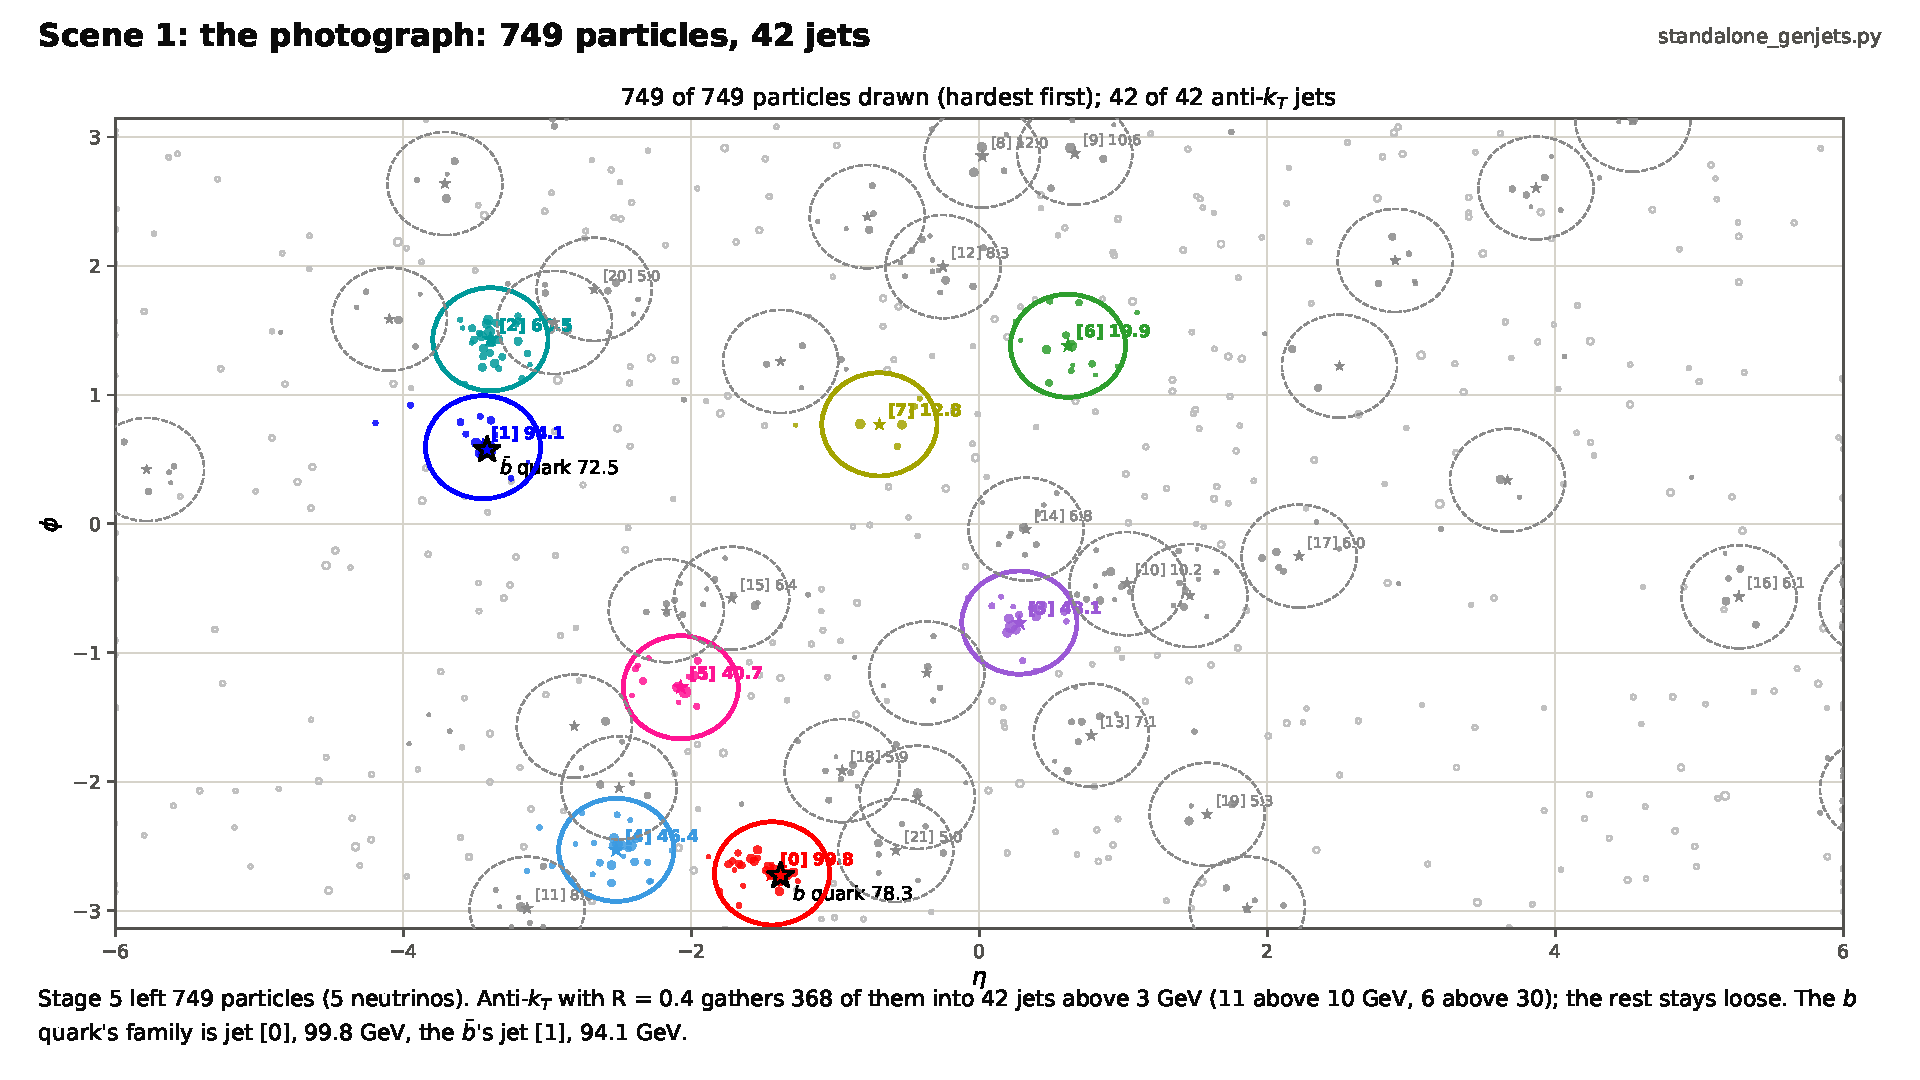
\includegraphics[page=1,width=0.325\textwidth]{GenJet/Standalone/animate_standalone_genjets_stills.pdf}\hfill
\includegraphics[page=2,width=0.325\textwidth]{GenJet/Standalone/animate_standalone_genjets_stills.pdf}\hfill
\includegraphics[page=3,width=0.325\textwidth]{GenJet/Standalone/animate_standalone_genjets_stills.pdf}\\[1.5mm]
\includegraphics[page=4,width=0.325\textwidth]{GenJet/Standalone/animate_standalone_genjets_stills.pdf}\hfill
\includegraphics[page=5,width=0.325\textwidth]{GenJet/Standalone/animate_standalone_genjets_stills.pdf}\hfill
\includegraphics[page=6,width=0.325\textwidth]{GenJet/Standalone/animate_standalone_genjets_stills.pdf}
\caption[Key frames of the animated standalone GenJet stage]{Key frames of
the six scenes of the animated standalone GenJet stage, drawn by
\file{animate_standalone_genjets.py} with \code{--stills}, in reading
order. The 749 particles and the 42 jets; \antikt building our jet merge
by merge; the radius, the neutrinos and the threshold; the ghosts and the
labels of the three $b$ jets; the soft $b\bar b$ pair and its
neutralisation; the response over four hundred decays. The film itself is the
seventh on the playlist of \jitjetworld.}
\label{fig:family_photograph:stills}
\end{figure}

\paragraph{The picture to carry: the photograph.}
The family of
\cref{fig:family_photograph:photograph_sketch} is what the decays left:
fifteen particles from the \Bbar within a tenth of a unit of each other,
sixteen more from the gluons and the underlying event within $0.4$, and a
scatter of soft particles everywhere. The photograph is a rule for
drawing a circle around them. \antikt draws it from the inside out, the
hardest particle first and everything within $R$ of it next, so that the
circle is round and centred on the hard core, and a soft particle at the
edge belongs or does not belong by its distance to that core alone. Two
things in the picture matter for everything that follows. The circle is
a choice three times over: its radius, $0.4$ for the small jets of this
book and $0.8$ for the boosted ones of \cref{ch:three_families}; whether
the neutrino inside it is counted, which CMS does not, because the
detector will not see it and a calibration against a photograph with
neutrinos would ask the detector to measure what it cannot; and the
threshold below which a circle is not a jet at all, $3\GeV$ for the
generator and $30$ or more for an analysis. And the label on the picture,
``$b$ jet'', is a second rule, laid on top of the first, which the
experiment answers with the B~hadron's ghost and the theory with a
definition that a soft gluon cannot change. The rules are the \antikt
paper~\cite{Cacciari:2008gp} and the \FASTJET manual~\cite{Cacciari:2011ma},
the \CMSSW producers \code{GenJetParticles}, \code{FastjetJetProducer}
and \code{JetFlavourClustering}, and, for the last section, the
flavour-$k_T$ of Banfi, Salam and Zanderighi~\cite{Banfi:2006hf} and the
interleaved flavour neutralisation of Caola, Grabarczyk, Hutt, Salam,
Scyboz and Thaler~\cite{Caletti:2022glq}. The algorithms themselves, their
history and the choice of $R$, are the business of \cref{ch:the_inn}; this
stop uses \antikt as the experiment's photographer and asks what the
photograph shows.

\begin{figure}[htbp]\centering
\resizebox{\textwidth}{!}{% ---------------------------------------------------------------------------
% The family photograph: (a) the b family of our event at stage 5 (the final
% particles of the Bbar0 and the neighbours within the cone) with the three
% photographs anti-kT takes of it, R = 0.4 with and without the neutrino and
% R = 0.8; (b) the three choices that change the picture but not the family.
% Numbers: event_GenJet.lhe (seed 1), the ensemble of 400 decays, and the
% CMSSW event (pages 6-8 of genJetAnalyzer_ME_PS_MPI_Had_Decay_GenJet_out.pdf).
% ---------------------------------------------------------------------------
\begin{tikzpicture}[x=1cm,y=1cm,
  every node/.style={font=\footnotesize},
  lab/.style={font=\scriptsize,align=center},
  head/.style={font=\small\bfseries},
  fam/.style={circle,fill=red!75!black,inner sep=0pt},
  oth/.style={circle,fill=black!40,inner sep=0pt},
  nu/.style={circle,draw=green!50!black,thick,fill=white,inner sep=0pt},
  ring4/.style={red!80!black,line width=1.6pt},
  ring8/.style={blue!70!black,line width=1.2pt,dashed},
  box/.style={draw,rounded corners=3pt,thin,fill=gray!6,align=left,inner sep=5pt,text width=5.0cm,font=\scriptsize}]
% ---------------- (a) the family and its photographs --------------------------------------------
\begin{scope}
\node[head,anchor=west] at (-4.4,4.6) {(a) the $b$ family at stage 5 and the photographs anti-$k_T$ takes of it};
% the (eta, phi) frame, 1 unit = 3 cm
\draw[-{Stealth}] (-4.0,-3.6) -- (4.0,-3.6) node[below left,lab] {$\eta$};
\draw[-{Stealth}] (-4.0,-3.6) -- (-4.0,3.9) node[left,lab] {$\phi$};
\foreach \x in {-3,-1.5,0,1.5,3} {\draw (\x,-3.65) -- (\x,-3.55);}
\foreach \y in {-3,-1.5,0,1.5,3} {\draw (-4.05,\y) -- (-3.95,\y);}
\node[lab,anchor=north] at (0,-3.7) {$0.5$ units of $\Delta R$ per tick};
% the rings
\draw[ring8] (0,0) circle (2.4);
\draw[ring4] (0,0) circle (1.2);
\node[lab,text=red!80!black,anchor=south west] at (0.85,0.85) {$R=0.4$: $99.83\,\mathrm{GeV}$, 31 particles};
\node[lab,text=blue!70!black,anchor=south west] at (1.7,1.75) {$R=0.8$: $105.79\,\mathrm{GeV}$, 47};
% the family: the Bbar0's 15 final descendants (red), the core very close
\foreach \p/\s in {(0.05,0.1)/5.5,(-0.1,-0.05)/4.5,(0.15,-0.15)/4.0,(-0.2,0.2)/3.2,(0.3,0.05)/3.0,(-0.05,0.35)/2.6,(0.25,-0.35)/2.4,(-0.4,-0.2)/2.2,(0.45,0.3)/2.0,(-0.35,0.5)/1.8,(0.55,-0.1)/1.6,(0.1,-0.6)/1.5,(-0.6,0.1)/1.4,(0.7,0.5)/1.3,(-0.5,-0.6)/1.2} {\node[fam,minimum size=\s pt] at \p {};}
% the neighbours inside R = 0.4 (grey), the periphery
\foreach \p/\s in {(0.9,0.6)/2.0,(-0.95,0.4)/1.8,(0.6,-0.9)/1.6,(-0.7,-0.8)/1.5,(1.05,-0.2)/1.4,(-0.3,1.0)/1.3,(0.2,1.1)/1.2,(-1.1,-0.1)/1.2,(0.95,-0.65)/1.1,(-0.8,0.85)/1.1,(0.4,-1.1)/1.0,(-0.15,-1.05)/1.0,(1.1,0.3)/1.0,(-1.0,-0.55)/1.0,(0.75,1.0)/0.9,(-0.55,1.05)/0.9} {\node[oth,minimum size=\s pt] at \p {};}
% between 0.4 and 0.8: the gluon's family and more soft stuff
\foreach \p/\s in {(1.6,0.9)/2.6,(1.9,0.5)/2.0,(1.5,1.4)/1.6,(2.1,1.1)/1.4,(-1.7,-1.2)/1.3,(-1.9,0.6)/1.2,(0.5,-2.0)/1.2,(-0.4,2.1)/1.1,(2.2,-0.7)/1.1,(-2.1,-0.4)/1.0,(1.2,-1.8)/1.0,(-1.3,1.7)/1.0,(0.9,2.1)/0.9,(-2.0,1.3)/0.9,(1.8,-1.4)/0.9,(-0.9,-2.1)/0.9} {\node[oth,minimum size=\s pt] at \p {};}
% outside
\foreach \p/\s in {(3.2,1.5)/1.4,(-3.1,-2.4)/1.2,(2.9,-2.6)/1.3,(-2.9,2.6)/1.1,(3.4,-0.6)/1.0,(-3.4,0.9)/1.0,(1.0,3.2)/1.0,(-1.4,-3.1)/1.0,(3.1,3.0)/0.9,(-3.3,-1.0)/0.9} {\node[oth,minimum size=\s pt] at \p {};}
% the quark and the axis
\node[star,star points=5,draw=black,fill=white,inner sep=1.4pt] at (-0.17,-0.06) {};
\node[lab,anchor=north east] at (-0.2,-0.2) {$b$ quark, $78.3$};
\node[star,star points=5,fill=red!80!black,inner sep=1.3pt] at (0,0) {};
% the neutrino of the semileptonic decay (seed 4), hollow
\node[nu,minimum size=6pt] at (-0.3,-0.4) {};
\node[lab,text=green!50!black,anchor=north east,align=right] at (-0.4,-0.5) {$\nu$ of decay seed 4:\\ $9.5\,\mathrm{GeV}$, in the ring,\\ not in the detector};
\node[lab,anchor=south west,text width=4.1cm,align=left,text=black!65] at (-4.0,-3.4) {red: the $\bar B^0$'s descendants, $78.3\,\mathrm{GeV}$;\\ grey: the rest of the event; the axis (red star) is the jet's, $0.06$ from the quark};
\end{scope}
% ---------------- (b) the choices ------------------------------------------------------------------
\begin{scope}[xshift=10.2cm]
\node[head,anchor=west] at (-0.6,4.6) {(b) three choices change the picture, not the family};
\node[box,anchor=north west] (C1) at (-0.6,3.9) {\textbf{the radius $R$}\\ $0.4$: $99.83\,\mathrm{GeV}$ (ak4GenJets)\\ $0.8$: $105.79\,\mathrm{GeV}$ (ak8GenJets)\\ the cone around the quark: $99.43$ and $108.73$\\ beyond $R\simeq1$ the neighbouring gluon jet is swallowed};
\node[box,anchor=north west,below=4mm of C1.south west] (C2) {\textbf{the neutrinos}\\ ak4GenJets keeps them, ak4GenJetsNoNu does not\\ our event: the same jet ($99.83$), no neutrino\\ decay seed 4 of the same hadrons: $99.6\to90.2$\\ 400 decays: $99.63\pm0.49\to91.93\pm12.12$\\ CMSSW's event: $117.8\to79.8$ ($37.5\,\mathrm{GeV}$ of $\nu$)};
\node[box,anchor=north west,below=4mm of C2.south west] (C3) {\textbf{the threshold}\\ jets above $3\,\mathrm{GeV}$ (GenJet): 42\\ above $10$: 11; above $30$: 6\\ CMSSW's event: 27 jets above $3\,\mathrm{GeV}$};
\node[lab,anchor=north west,text width=5.2cm,align=left,text=black!65,below=4mm of C3.south west] {Every later chapter compares a reconstructed jet with one of these photographs and must say which: CMS calibrates to the one without neutrinos.};
\end{scope}
\end{tikzpicture}
}
\caption[The family photograph: the $b$ family and the pictures anti-$k_T$
takes of it]{The family photograph. Left: the $b$ family of our event at
stage~5, the fifteen descendants of the \Bbar ($b\bar d$) in red and the
rest of the event in grey around the jet axis, with the two circles that
\antikt draws, $R=0.4$ and $0.8$, and the neutrino of decay seed~4 of the
ensemble, which sits inside the ring and outside the detector. Right: the
three choices that change the picture but not the family, with the
numbers of our event, of four hundred decays and of the \CMSSW event.}
\label{fig:family_photograph:photograph_sketch}
\end{figure}

\paragraph{The number, four ways.}
\label{sec:family_photograph:validation}
\label{sec:family_photograph:standalone_code}
\Cref{tab:family_photograph:numbers} gives away the ending. The sharpest
column pair is, once more, a comparison on identical input: the 749
particles of \file{event_Decay.lhe} clustered by \FASTJET~3.5.2 and by the
script, with the same ghosts. They agree exactly, to the last digit of
every jet momentum and to the last constituent, which is what a port of a
deterministic algorithm must do; the interesting columns are the ones
that vary, the four hundred decays of the same hadrons clustered each
time, \PYTHIA's full chain with \FASTJET, and the \CMSSW event.

The standalone script writes out what the \code{GenJet} producers of
\CMSSW do with \FASTJET, what the \code{JetFlavourClustering} module does
afterwards, and adds the two infrared-safe flavour definitions of the
literature; it imports the decay script of
\cref{ch:children_producing_grandchildren} for the record and the
particle names. Its learning mode, \code{-v}, prints the ghosts with their
rows and momenta, then the $36$ merges that built the $b$ quark's \akfour
jet in the order the algorithm made them, each with its distance, its
\dR, the two momenta and the merged one, the labels of the two $b$ jets
with their ghosts, the IFN pass and the
flavoured merges of flavour-$k_T$; \code{-vv} adds every one of the $928$
steps of the clustering. The \code{-v} log for seed~1 is committed, and
every number quoted in the theory of this chapter is taken from it.
\label{sec:family_photograph:fastjet}

The first official check is not statistical. \FASTJET, the library every
experiment calls, is driven from a script on the $749$ particles of
\file{event_Decay.lhe} with the same $179$ ghosts as \code{PseudoJet}s and
the E~scheme for the three collections, and \PYTHIA's own \code{SlowJet},
with the \code{fjcore} of \FASTJET inside, clusters the same particles
from a filled event record. Not a single jet, constituent or label
differs: $42$, $42$ and $30$ jets in the three collections, the momenta
identical to the last digit, the constituent lists identical, the three
labels identical, and the same for $k_T$ and Cambridge/Aachen; \code{SlowJet}
agrees to the rounding of a double. This is the first stop of the journey
at which the agreement is exact rather than statistical, and it should
be: the algorithm is deterministic and leaves nothing to tune. The second
official source is \PYTHIA's full chain, two thousand events with the
shower, the secondary scatterings and the decays all varying, clustered
by \FASTJET with the ghosts and the status-71 copy of each quark as the
axis, the choice of the \CMSSW analyser: $18.2\pm11.5$ \akfour jets above
$3\GeV$ against the $40.0$ of the fixed hadrons of the ensemble, because
the number of secondary scatterings varies and our event has many; the
mother's jet at $109.9\pm27.6\GeV$ for a quark of $95.5\pm30$, the
response $1.22\pm0.51$ with a median of $1.06$, wide because the
status-71 quark itself is soft whenever a hard gluon left it so;
$7.9\GeV$ of neutrinos in the jet on average and none in $58\%$ of the
events; \hadflav $5$ in $99.2\%$. The structure is that of the ensemble,
and the numbers that the ensemble holds fixed, the shower and the
underlying event, are what the full chain spreads.
\label{sec:family_photograph:cmssw}

The third official check costs nothing to generate: the \code{GEN} step of
\cref{sec:ancestral_home:cmssw} runs the \code{genJetParticles} and
\code{recoGenJets} sequences after the hadron level, so that every GEN
file carries \akfour, \akfournonu and \akeight already, made by
\code{FastjetJetProducer} with \FASTJET's \antikt, the E scheme and
\code{jetPtMin = 3}; the flavour producers run later, in the \code{PAT}
step, and are not in the GEN output. For this stop the same producers are
run once more as a step of their own on the complete event of
\cref{ch:children_producing_grandchildren}, so that the jets can be read
and drawn. Its event is the last column of the table, and
\cref{sec:family_photograph:our_jet_at_this_stage_the_reference_genj} reads
its \akfour page next to the standalone one. How each column was
produced, the commands, the modes and the logs, is in the companion of
this chapter,
\begin{center}
  \companion{chapter_07_GenJet}
\end{center}
together with the full tables behind every number quoted below.

\begin{table}[htbp]\centering\small
\caption[Generator-level jets obtained four ways]{Generator-level jets
obtained four ways. ``Same particles'' means the 749 final particles of
\file{example/Decay/event_Decay.lhe} with the same ghosts, clustered by
\FASTJET~3.5.2 and by the standalone script; ``400 decays'' means the
primary hadrons of \cref{ch:children_getting_married} decayed four hundred
times with the script of \cref{ch:children_producing_grandchildren} and
clustered each time; ``full chain'' means \PYTHIA from the hard event of
\cref{ch:ancestral_home} with the CP5 settings, $2000$ events, clustered
with \FASTJET and the same ghosts, the status-71 copy of the quark as the
axis. The spread of a single event follows $\pm$. ``Response'' is
$\pt(\mathrm{jet})/\pt(b)$ with the last copy of the quark before the
hadronisation, which in the full chain fluctuates itself. The \CMSSW
column is the single event of \cref{ch:ancestral_home}, read from the log
of its jet analyser.}
\label{tab:family_photograph:numbers}
\scriptsize\setlength{\tabcolsep}{3pt}
\resizebox{\textwidth}{!}{%
\begin{tabular}{lrrrrr}\toprule
 & \FASTJET & standalone & standalone & \PYTHIA + \FASTJET & \CMSSW \\
 & same particles & same particles & 400 decays & full chain & 1 event \\ \midrule
\akfour: jets above $3$ / $10$ / $30\GeV$ & $42$ / $11$ / $6$ & $42$ / $11$ / $6$ & $40.0\pm2.2$ / $10.2$ / $6.0$ & $18.2\pm11.5$ / $3.9$ / $2.4$ & $27$ / $6$ / $2$ \\
\quad particles clustered, of & $368$ of $749$ & $368$ of $749$ & $357\pm16$ & $152\pm88$ & $239$ of $634$ \\
\akeight: jets, particles clustered & $30$, $600$ & $30$, $600$ & $30.4$, $608$ & $20.2$, $321$ & $28$, $488$ \\ \midrule
$b$ quark (last copy): \pt [GeV] & $78.29$ & $78.29$ & $78.29$ & $95.5\pm30.0$ & $91.74$ \\
$b$ jet, \akfour: \pt [GeV], $n$ & $99.830$, $31$ & $99.830$, $31$ & $99.63\pm0.49$, $25.7$ & $109.9\pm27.6$, $21.3$ & $117.79$, $24$ \\
\quad response, \dR to the quark & $1.275$, $0.062$ & $1.275$, $0.062$ & $1.273\pm0.006$, $0.060$ & $1.22\pm0.51$, $0.028$ & $1.284$, $0.019$ \\
\quad the cone of the same $R$ [GeV] & $99.43$ & $99.43$ & $98.79\pm0.68$ & $109.7\pm26.5$ & $79.12$ (no $\nu$) \\
\quad neutrino \pt inside [GeV] & $0$ & $0$ & $7.7$ (none in $54\%$) & $7.9$ (none in $58\%$) & $37.5$ \\
$b$ jet, \akfournonu: \pt [GeV] & $99.830$ & $99.830$ & $91.93\pm12.12$ & $102.1\pm28.9$ & $79.82$ \\
$b$ jet, \akeight: \pt [GeV], $n$ & $105.786$, $47$ & $105.786$, $47$ & $104.61\pm0.80$, $41.3$ & $120.0\pm24.6$, $34.3$ & $141.10$, $55$ \\
$b$ jet: \hadflav $=5$, $|\partflav|=5$ [\%] & $5$, $5$ & $5$, $5$ & $100$, $100$ & $99.2$, $99.3$ & -- \\
$b$ jet: physics flavour, $\dR<0.3$ flavour & $0$, $+5$ & $0$, $+5$ & -- & -- & -- \\
$b$ jet: net $b$ flavour $+1$ / $-1$ [\%] & $+1$ & $+1$ & $83.2$ / $16.8$ & -- & -- \\
$b$ jet: B hadron to the axis, its products outside & $0.06$, $0$ & $0.06$, $0$ & $0.062$, $0.20$ & $0.025$, $0.31$ & -- \\ \midrule
$\bar b$ jet, \akfour: \pt [GeV], response & $94.093$, $1.298$ & $94.093$, $1.298$ & $93.86\pm0.83$, $1.295$ & $106.5\pm20.9$, $1.23$ & $115.94$, $0.996$ \\
$\bar b$ jet, \akeight: \pt [GeV], \dR & $147.688$, $0.361$ & $147.688$, $0.361$ & $113.4\pm20.4$, $0.14$ & $115.3\pm17.0$, $0.05$ & $121.01$, $0.022$ \\
$\bar b$ jet: net $b$ flavour $-1$ / $+1$ [\%] & $+1$ (oscillated) & $+1$ (oscillated) & $79.2$ / $20.8$ & -- & -- \\
\akfour jets with two $b$ hadrons per event & $1$ & $1$ & $1.00$ & $0.009$ & -- \\
IFN neutralisations per event & $0$ & $0$ & $0.66$ & -- & -- \\
\bottomrule
\end{tabular}}
\end{table}

\section{Let us dive into the details: the theory}
\label{sec:family_photograph:theory}

\subsection{What we mean by ``the true jet'': choices and their consequences}
\label{sec:family_photograph:what_we_mean_by_the_true_jet_choices_and}

A photograph is a rule, and the rule has a distance, a radius, a list of
who may be in the picture and a threshold. The distance first, because it
is the part the newcomer least expects to matter, and because three
different distances are in use at the LHC, each taking a different
picture of the same family. I take nine particles of our event and let
each of the three photographers cluster them in front of you, step by
step; then the real jet of thirty-one; then the whole event under the
three rules, which is where you will see why the experiments chose
\antikt for the photograph of every chapter to come.

\subsubsection{Three photographers, nine particles: the clustering step by step}
\label{sec:family_photograph:nine_particles}

Guess first. Here are nine particles of the record, \cref{tab:family_photograph:nine}:
four of the core of our $b$ jet, two pairs that happen to be very close,
three soft particles at its border, and the leading particle of each of
the two nearest other jets. Which of the nine end up together, and in
which order are they gathered? Three scripts in
\file{example/GenJet/Standalone/} answer with every distance printed (the
companion gives the commands and the full logs), and all three treat the particles as massless, so that rapidity and
pseudorapidity coincide, and add four-momenta when they merge (the
E~scheme). Every sequential recombination algorithm has the same shape:
a distance \dij between any two of the objects alive, a distance \diB of
each object to the beam, and the rule that at every step the smallest of
them all wins, a pair being merged into one object, or an object being
declared a jet and set aside, until nothing is left. The generalised-$k_T$
family~\cite{Catani:1993hr,Ellis:1993tq,Dokshitzer:1997in,Wobisch:1998wt,Cacciari:2008gp}
writes
\begin{equation}
  \dij=\min\!\big(p_{T,i}^{2p},\,p_{T,j}^{2p}\big)\,\frac{\dR_{ij}^2}{R^2},\qquad
  \diB=p_{T,i}^{2p},\qquad
  \dR_{ij}^2=(y_i-y_j)^2+(\phi_i-\phi_j)^2,
  \label{eq:family_photograph:genkt}
\end{equation}
and the power $p$ is the whole difference between its members: $p=-1$ is
\antikt, $p=0$ Cambridge/Aachen, $p=1$ the original $k_T$ algorithm,
which \cref{ch:the_inn} takes up. HOTVR keeps the Cambridge/Aachen
ordering and changes the beam distance and the merge.

\begin{table}[htbp]\centering\small
\caption[The nine particles of the clustering example]{The nine particles
of \file{antiKt.py}, \file{caKt.py} and \file{hotVR.py}: rows of the
record with their \pt, $\eta$ and $\phi$, and where each sits in the
event. $\dR$ to the core is measured from the \pt-weighted centre of
A--D, $(-1.362,-2.741)$.}
\label{tab:family_photograph:nine}
\resizebox{\textwidth}{!}{%
\begin{tabular}{llrrrll}\toprule
 & particle & \pt [GeV] & $\eta$ & $\phi$ & $\dR$ to the core & where \\\midrule
A & $\pi^+$ [2181] & 14.27 & $-1.336$ & $-2.721$ & 0.03 & the hardest particle of the $b$ jet \\
B & $\pi^-$ [2239] & 5.41 & $-1.359$ & $-2.712$ & 0.03 & $0.025$ from A \\
C & $K^-$ ($s\bar u$) [2211] & 10.57 & $-1.389$ & $-2.770$ & 0.04 & the $D^0$'s kaon \\
D & $\pi^-$ [2241] & 4.45 & $-1.383$ & $-2.770$ & 0.04 & $0.006$ from C: the first merge of our jet \\
E & $\pi^+$ [1217] & 0.68 & $-1.801$ & $-2.849$ & 0.45 & the last particle \antikt added to our real jet \\
F & $\gamma$ [1538] & 1.86 & $-1.741$ & $-2.641$ & 0.39 & at the border \\
G & $\gamma$ [2183] & 0.97 & $-1.713$ & $-2.616$ & 0.37 & $0.037$ from F; E is $0.23$ from the pair \\
H & $\Lambda^0$ ($uds$) [1546] & 8.28 & $-2.417$ & $-2.496$ & 1.08 & the leading particle of the gluon jet [4] \\
I & $\pi^+$ [1592] & 24.57 & $-2.043$ & $-1.304$ & 1.59 & the leading particle of jet [5] \\
\bottomrule
\end{tabular}}
\end{table}

\paragraph{Anti-$k_T$: the hard one sets every distance}

With $p=-1$ the minimum in \cref{eq:family_photograph:genkt} picks the
\emph{larger} momentum, $\dij=\max(\pt)^{-2}\,\dR^2/R^2$, and
$\diB=\pt^{-2}$: a hard particle is close to everything within $R$ of
itself, at a distance that does not know the other particle's momentum,
and it is far from the beam only while something is still inside its
circle.
The nine steps of the script, every distance of which the companion
prints, are: $C+D$, then $A+B$, then the two cores into one object of
$34.69\GeV$ (steps~1 to~3); G at $\dR=0.373$ and F at $0.382$ at the
core's distance (steps~4 and~5); the core declared a jet of six particles
and $37.50\GeV$ when its beam distance wins (step~6); and I, H and E
declared alone, in that order (steps~7 to~9).
Read the first line with the formula: $K^-$ and $\pi^-$ are $0.006$
apart and the kaon has $10.57\GeV$, so
$\dij=10.57^{-2}\times(0.006/0.4)^2=2.1\times10^{-6}$, while the hardest
pair in the event, A and B at $0.025$, has
$14.27^{-2}\times(0.025/0.4)^2=1.9\times10^{-5}$: the closer pair wins
although it is softer, because $0.006^2$ beats $0.025^2$ by more than
$10.57^2$ loses to $14.27^2$. Once the two cores are one object of
$34.69\GeV$ its beam distance is $34.69^{-2}=8.3\times10^{-4}$, and every
particle within $R$ of it is closer than that: G at $0.373$ gives
$8.3\times10^{-4}\times(0.373/0.4)^2=7.2\times10^{-4}$, F at $0.382$ the
same to two digits, and neither $0.97$ nor $1.86\GeV$ appears anywhere in
those numbers. E does not come: it is $0.43$ from the axis after F has
moved it, so $\dij$ to the core exceeds the core's \diB, the core is
declared a jet at step~6 with six particles and $37.50\GeV$, and E is
left to be a jet of its own at step~9, which the $3\GeV$ threshold of
\cref{sec:family_photograph:choices} would drop. I and H are declared
in order of their own $\pt^{-2}$, each alone.

\paragraph{Cambridge/Aachen: the angle alone}

With $p=0$ the momenta vanish from \cref{eq:family_photograph:genkt},
$\dij=\dR^2/R^2$ and $\diB=1$: the closest pair in angle is merged first
whatever its momenta, and an object is a jet once nothing is left within
$R$ of it.
The nine steps are now: $C+D$, $A+B$, then $F+G$ at $0.037$ before
the two cores have found each other (steps~1 to~3); the cores (step~4);
E joins the photon pair at $0.228$ (step~5); the blob of $3.49\GeV$ joins
the core at $0.389$ (step~6); and H, I and the jet ABCDEFG of $38.18\GeV$
are declared (steps~7 to~9).
The two photons, $0.037$ apart, pair up at step~3 before the two cores
have found each other, E joins their blob at $0.228$ (step~5), and the
blob of $3.49\GeV$, whose centre is $0.389$ from the core, is merged
whole at step~6: E, which \antikt left out, is in the jet, carried in by
two photons it was close to. The hard jets are the same, the border is
not: it follows the soft particles, and a soft particle on the far side
of a soft neighbour can enter, or a soft particle inside can be pulled
out by one further away. This angle-ordered sequence is exactly what
makes Cambridge/Aachen the tool of jet \emph{substructure}, where one
reclusters the constituents of a jet to find the structure inside, and
its weakness as the photograph of the family.

\paragraph{HOTVR: a radius that shrinks with momentum, and a mass test}

The Heavy Object Tagger with Variable~R~\cite{Lapsien:2016zor}, built on
the variable-$R$ idea of \cite{Krohn:2009zg}, keeps the Cambridge/Aachen
ordering, $\dij=\dR_{ij}^2$, and lets the beam distance depend on the
object,
\begin{equation}
  \diB=R_{\mathrm{eff}}(\pt)^2,\qquad
  R_{\mathrm{eff}}=\mathrm{clip}\!\big(\rho/\pt,\;R_{\min},\;R_{\max}\big),
  \label{eq:family_photograph:hotvr}
\end{equation}
so that a boosted object of large \pt is photographed in a small circle
and a slow one in a large one; and before every merge whose combined
mass exceeds $\mu$ it asks whether the merge is a real \emph{mass jump},
$\theta\,m_{ij}>\max(m_i,m_j)$, with both branches above $p_{T,\mathrm{sub}}$:
if the jump fails the lighter branch is thrown away, if a branch is too
soft it is thrown away, and only a jump between two hard branches is
merged, the two branches remembered as subjets. The paper's values are
for top quarks, $\rho=600\GeV$, $R_{\mathrm{eff}}\in[0.1,1.5]$,
$\mu=30\GeV$, $\theta=0.7$, $p_{T,\mathrm{sub}}=30\GeV$, and for our
nine particles, none above $400\GeV$, every $R_{\mathrm{eff}}$ is $1.5$:
The script's nine steps are the six merges of Cambridge/Aachen with
every pair mass below $\mu$; then H merged at $\dR=1.047$ with
$m_{ij}=20.1\GeV$, still below $\mu$ (step~7); then I at $1.459$, where
the mass jump passes, $m_{ij}=52.2>\mu$ and $0.7\times52.2=36.5>20.1$, but
I has $\pt=24.6<p_{T,\mathrm{sub}}$ and the soft branch is discarded
(step~8); and the jet finalised at $46.3\GeV$ with $m=20.1$ and
$R_{\mathrm{eff}}=1.5$ (step~9).
Then the circle of $1.5$ reaches the gluon jet's $\Lambda^0$ at
$1.05$, and since the pair mass is $20.1\GeV$, still below $\mu$, H is
merged like any other particle: the photograph now holds a piece of the
neighbouring family. Jet [5]'s pion at $1.46$ is next, and this time
$m_{ij}=52.2\GeV$ passes $\mu$, the jump $0.7\times52.2=36.5$ exceeds the
$20.1$ of the heavier branch, but the pion's $24.6\GeV$ is below
$p_{T,\mathrm{sub}}$: I is thrown away, not merged and not left alone,
and the jet is declared with $46.3\GeV$ in eight particles. That is the
grooming HOTVR does in the clustering itself, where the top tagger wants
it; for a $100\GeV$ $b$ family it is the wrong lens.

\paragraph{What each of them clusters in the end.}
\Cref{tab:family_photograph:three_results} and
\cref{fig:family_photograph:three_trees} put the three sequences side by
side; \cref{fig:family_photograph:nine_pictures} shows the pictures the
scripts draw.
\begin{table}[htbp]\centering\small
\caption[The three algorithms on the nine particles: the result]{What
the three photographers make of the nine particles. The steps are the
scripts' logs; jets below the $3\GeV$ threshold of \CMSSW are in
brackets.}
\label{tab:family_photograph:three_results}
\begin{tabular}{p{3.9cm}p{3.9cm}p{4.4cm}}\toprule
\antikt, $R=0.4$ & Cambridge/Aachen, $R=0.4$ & HOTVR (paper's parameters) \\\midrule
C+D, A+B, cores, then G and F at the core's distance; E stays out &
C+D, A+B, F+G, cores, E joins F+G, the blob joins the core &
as Cambridge/Aachen, then H at $1.05$ ($m=20<\mu$), I at $1.46$ groomed away ($m=52>\mu$, $\pt<p_{T,\mathrm{sub}}$) \\[2pt]
\textbf{ABCDFG} $37.50\GeV$ \newline I $24.57$, H $8.28$, (E $0.68$) &
\textbf{ABCDEFG} $38.18\GeV$ \newline I $24.57$, H $8.28$ &
\textbf{ABCDEFGH} $46.3\GeV$, $R_{\mathrm{eff}}=1.5$, $m=20\GeV$ \newline I thrown away \\[2pt]
round, the border set by the hard core & the border follows the soft particles & one fat jet of two families, groomed \\
\bottomrule
\end{tabular}
\end{table}

\begin{figure}[htbp]\centering
\resizebox{\textwidth}{!}{% ---------------------------------------------------------------------------
% Nine particles of our event (antiKt.py, caKt.py, hotVR.py) clustered by the
% three rules: the order of the merges as a tree, bottom to top, with the
% winning distance at every step. A: pi+ 14.3 GeV, B: pi- 5.4 (0.025 from A),
% C: K- 10.6, D: pi- 4.5 (0.006 from C), E: pi+ 0.7, F: gamma 1.9, G: gamma 1.0
% (F, G 0.037 apart at the border; E 0.23 from them), H: Lambda0 8.3 (the gluon
% jet [4], 1.1 away), I: pi+ 24.6 (jet [5], 1.6 away). Numbers: the three logs.
% Three panels stacked; y = 0.45 x step.
% ---------------------------------------------------------------------------
\begin{tikzpicture}[x=1cm,y=1cm,
  every node/.style={font=\footnotesize},
  lab/.style={font=\scriptsize,align=center},
  dval/.style={font=\tiny,text=black!70,anchor=west,inner sep=1pt,text width=6.6cm,align=left},
  expl/.style={font=\scriptsize,anchor=north west,text width=3.1cm,align=left},
  head/.style={font=\small\bfseries,anchor=west},
  leaf/.style={font=\scriptsize\bfseries,anchor=north},
  hard/.style={circle,fill=red!75!black,inner sep=0pt},
  soft/.style={circle,fill=black!45,inner sep=0pt},
  oth/.style={circle,fill=blue!60!black,inner sep=0pt},
  tree/.style={red!80!black,thick},
  treeb/.style={blue!60!black,thick},
  jet/.style={star,star points=5,fill=black,inner sep=1.4pt},
  groom/.style={black!60,thick,dashed}]
% leaves: C D A B G F E H I at x = 0, 0.7, ..., with a marker scaled by pT
\newcommand{\leaves}{%
  \node[hard,minimum size=6.5pt] at (0,0) {}; \node[leaf] at (0,-0.12) {C};
  \node[hard,minimum size=4.2pt] at (0.7,0) {}; \node[leaf] at (0.7,-0.12) {D};
  \node[hard,minimum size=7.5pt] at (1.4,0) {}; \node[leaf] at (1.4,-0.12) {A};
  \node[hard,minimum size=4.6pt] at (2.1,0) {}; \node[leaf] at (2.1,-0.12) {B};
  \node[soft,minimum size=2.0pt] at (2.8,0) {}; \node[leaf] at (2.8,-0.12) {G};
  \node[soft,minimum size=2.8pt] at (3.5,0) {}; \node[leaf] at (3.5,-0.12) {F};
  \node[soft,minimum size=1.7pt] at (4.2,0) {}; \node[leaf] at (4.2,-0.12) {E};
  \node[oth,minimum size=5.8pt] at (5.2,0) {}; \node[leaf] at (5.2,-0.12) {H};
  \node[oth,minimum size=10pt] at (6.2,0) {}; \node[leaf] at (6.2,-0.12) {I};
  \node[lab,anchor=north,text=black!60] at (3.1,-0.42) {$\underbrace{\hspace{2.0cm}}_{\text{the core, within }0.07}$\hspace{2mm}$\underbrace{\hspace{1.5cm}}_{\text{the border}}$\hspace{3mm}$\underbrace{\hspace{1.2cm}}_{\text{jets [4], [5]}}$};
  \draw[-{Stealth[length=1.6mm]},black!50] (-0.6,0.15) -- (-0.6,4.8) node[lab,anchor=south,text=black!60] {step};
  \foreach \k in {1,...,9} {\node[font=\tiny,text=black!50,anchor=east] at (-0.65,0.5*\k) {\k};}}
% ---------------- (a) anti-kT ---------------------------------------------------------------------
\begin{scope}
\node[head] at (-0.6,5.25) {(a) anti-$k_T$, $R=0.4$: \ \normalfont\footnotesize $d_{ij}=\min(p_{T,i}^{-2},p_{T,j}^{-2})\,\Delta R_{ij}^2/R^2$, \ $d_{iB}=p_{T,i}^{-2}$};
\leaves
\draw[tree] (0,0.15) -- (0,0.5) -- (0.7,0.5) -- (0.7,0.15);
\draw[tree] (1.4,0.15) -- (1.4,1) -- (2.1,1) -- (2.1,0.15);
\draw[tree] (0.35,0.5) -- (0.35,1.5) -- (1.75,1.5) -- (1.75,1);
\draw[tree] (1.05,1.5) -- (1.05,2) -- (2.8,2) -- (2.8,0.15);
\draw[tree] (1.9,2) -- (1.9,2.5) -- (3.5,2.5) -- (3.5,0.15);
\draw[tree] (2.7,2.5) -- (2.7,3); \node[jet,red!80!black] at (2.7,3.05) {};
\draw[treeb] (6.2,0.15) -- (6.2,3.5); \node[jet,blue!60!black] at (6.2,3.55) {};
\draw[treeb] (5.2,0.15) -- (5.2,4); \node[jet,blue!60!black] at (5.2,4.05) {};
\draw[black!50,thick] (4.2,0.15) -- (4.2,4.5); \node[jet,black!50] at (4.2,4.55) {};
\node[dval] at (6.7,0.5) {1: C+D at $\Delta R=0.006$: $d=10.57^{-2}(0.006/0.4)^2=2.1\cdot10^{-6}$};
\node[dval] at (6.7,1) {2: A+B at $0.025$: $d=14.27^{-2}(0.025/0.4)^2=1.9\cdot10^{-5}$};
\node[dval] at (6.7,1.5) {3: the two cores at $0.07$: $d=7.6\times10^{-5}$};
\node[dval] at (6.7,2) {4: G joins at $0.37$: $d=34.69^{-2}(0.37/0.4)^2=7.2\cdot10^{-4}$};
\node[dval] at (6.7,2.5) {5: F joins at $0.38$: $d=7.2\cdot10^{-4}$; F's $p_T$ never enters};
\node[dval] at (6.7,3) {6: $d_{iB}=1/37.5^2=7.1\times10^{-4}$: \textbf{jet ABCDFG}, $37.5$ GeV};
\node[dval] at (6.7,3.5) {7: $d_{iB}=1/24.6^2$: jet I};
\node[dval] at (6.7,4) {8: $d_{iB}=1/8.3^2$: jet H};
\node[dval] at (6.7,4.5) {9: $d_{iB}=1/0.68^2=2.2$: E alone, below $3$ GeV};
\node[expl] at (13.6,4.6) {The hard core sets every distance: G and F join at $d=p_{T,\mathrm{core}}^{-2}(\Delta R/R)^2$ whatever their own $p_T$; E, $0.43$ from the axis, does not. A round jet, the border decided by the core.};
\end{scope}
% ---------------- (b) Cambridge/Aachen ------------------------------------------------------------
\begin{scope}[yshift=-6.9cm]
\node[head] at (-0.6,5.25) {(b) Cambridge/Aachen, $R=0.4$: \ \normalfont\footnotesize $d_{ij}=\Delta R_{ij}^2/R^2$, \ $d_{iB}=1$};
\leaves
\draw[tree] (0,0.15) -- (0,0.5) -- (0.7,0.5) -- (0.7,0.15);
\draw[tree] (1.4,0.15) -- (1.4,1) -- (2.1,1) -- (2.1,0.15);
\draw[tree] (2.8,0.15) -- (2.8,1.5) -- (3.5,1.5) -- (3.5,0.15);
\draw[tree] (0.35,0.5) -- (0.35,2) -- (1.75,2) -- (1.75,1);
\draw[tree] (3.15,1.5) -- (3.15,2.5) -- (4.2,2.5) -- (4.2,0.15);
\draw[tree] (1.05,2) -- (1.05,3) -- (3.68,3) -- (3.68,2.5);
\draw[treeb] (5.2,0.15) -- (5.2,3.5); \node[jet,blue!60!black] at (5.2,3.55) {};
\draw[treeb] (6.2,0.15) -- (6.2,4); \node[jet,blue!60!black] at (6.2,4.05) {};
\draw[tree] (2.36,3) -- (2.36,4.5); \node[jet,red!80!black] at (2.36,4.55) {};
\node[dval] at (6.7,0.5) {1: C+D at $0.006$: $d=(0.006/0.4)^2=0.0002$};
\node[dval] at (6.7,1) {2: A+B at $0.025$: $d=0.004$};
\node[dval] at (6.7,1.5) {3: F+G at $0.037$: $d=0.009$: the photons pair up};
\node[dval] at (6.7,2) {4: the two cores at $0.07$: $d=0.029$};
\node[dval] at (6.7,2.5) {5: E joins F+G at $0.23$: $d=0.32$};
\node[dval] at (6.7,3) {6: the blob ($3.5$ GeV) joins the core at $0.39$: $d=0.94<1$};
\node[dval] at (6.7,3.5) {7: $d_{iB}=1$: jet H};
\node[dval] at (6.7,4) {8: $d_{iB}=1$: jet I};
\node[dval] at (6.7,4.5) {9: $d_{iB}=1$: \textbf{jet ABCDEFG}, $38.2$ GeV};
\node[expl] at (13.6,4.6) {Angle only: F and G pair up before the core is finished, E joins their blob, and the blob carries E into the jet. The same hard jets, a border that follows the soft particles.};
\end{scope}
% ---------------- (c) HOTVR -----------------------------------------------------------------------
\begin{scope}[yshift=-13.8cm]
\node[head] at (-0.6,5.25) {(c) HOTVR: \ \normalfont\footnotesize $d_{ij}=\Delta R_{ij}^2$, \ $d_{iB}=R_{\mathrm{eff}}^2$, \ $R_{\mathrm{eff}}=\mathrm{clip}(600\,\mathrm{GeV}/p_T,\,0.1,\,1.5)=1.5$ for all nine};
\leaves
\draw[tree] (0,0.15) -- (0,0.5) -- (0.7,0.5) -- (0.7,0.15);
\draw[tree] (1.4,0.15) -- (1.4,1) -- (2.1,1) -- (2.1,0.15);
\draw[tree] (2.8,0.15) -- (2.8,1.5) -- (3.5,1.5) -- (3.5,0.15);
\draw[tree] (0.35,0.5) -- (0.35,2) -- (1.75,2) -- (1.75,1);
\draw[tree] (3.15,1.5) -- (3.15,2.5) -- (4.2,2.5) -- (4.2,0.15);
\draw[tree] (1.05,2) -- (1.05,3) -- (3.68,3) -- (3.68,2.5);
\draw[tree] (2.36,3) -- (2.36,3.5) -- (5.2,3.5) -- (5.2,0.15);
\draw[groom] (6.2,0.15) -- (6.2,4) -- (3.78,4) -- (3.78,3.5);
\draw[black!60,thick] (6.05,3.85) -- (6.35,4.15) (6.05,4.15) -- (6.35,3.85);
\draw[tree] (3.78,4) -- (3.78,4.5); \node[jet,red!80!black] at (3.78,4.55) {};
\node[dval] at (6.7,0.5) {1--5: as Cambridge/Aachen, every pair mass far below $\mu=30$ GeV};
\node[dval] at (6.7,3) {6: the core takes E, F, G: $m=4.6$ GeV, a plain merge};
\node[dval] at (6.7,3.5) {7: H at $1.05<R_{\mathrm{eff}}$: $m_{ij}=20.1\le\mu$, \textbf{H merged}};
\node[dval] at (6.7,4) {8: I at $1.46$: $m_{ij}=52>\mu$, $\theta m_{ij}=36.5>20.1$, $p_T<p_{T,\mathrm{sub}}$: \textbf{I groomed}};
\node[dval] at (6.7,4.5) {9: $d_{iB}=1.5^2$: \textbf{jet ABCDEFGH}, $46.3$ GeV};
\node[expl] at (13.6,4.6) {With $\rho=600$ GeV everything below $400$ GeV has $R_{\mathrm{eff}}=1.5$: the gluon jet's $\Lambda^0$ is swallowed as an ordinary particle, and jet [5]'s pion, a mass jump, is thrown away as too soft. A photograph of a different object.};
\end{scope}
\end{tikzpicture}
}
\caption[The nine particles under the three algorithms, as trees]{The
order of the merges for the nine particles of
\cref{tab:family_photograph:nine}, bottom to top, with the winning
distance at every step (the logs of \file{antiKt.py}, \file{caKt.py} and
\file{hotVR.py}). Top: \antikt, the core first, then its neighbours at
the core's distance, E left out. Middle: Cambridge/Aachen, the closest
pair first whatever its momentum; F and G pair up, E joins them and is
carried into the jet. Bottom: HOTVR, the same order with $R_{\mathrm{eff}}=1.5$
and the mass test: H merged, I groomed away.}
\label{fig:family_photograph:three_trees}
\end{figure}

\begin{figure}[htbp]\centering
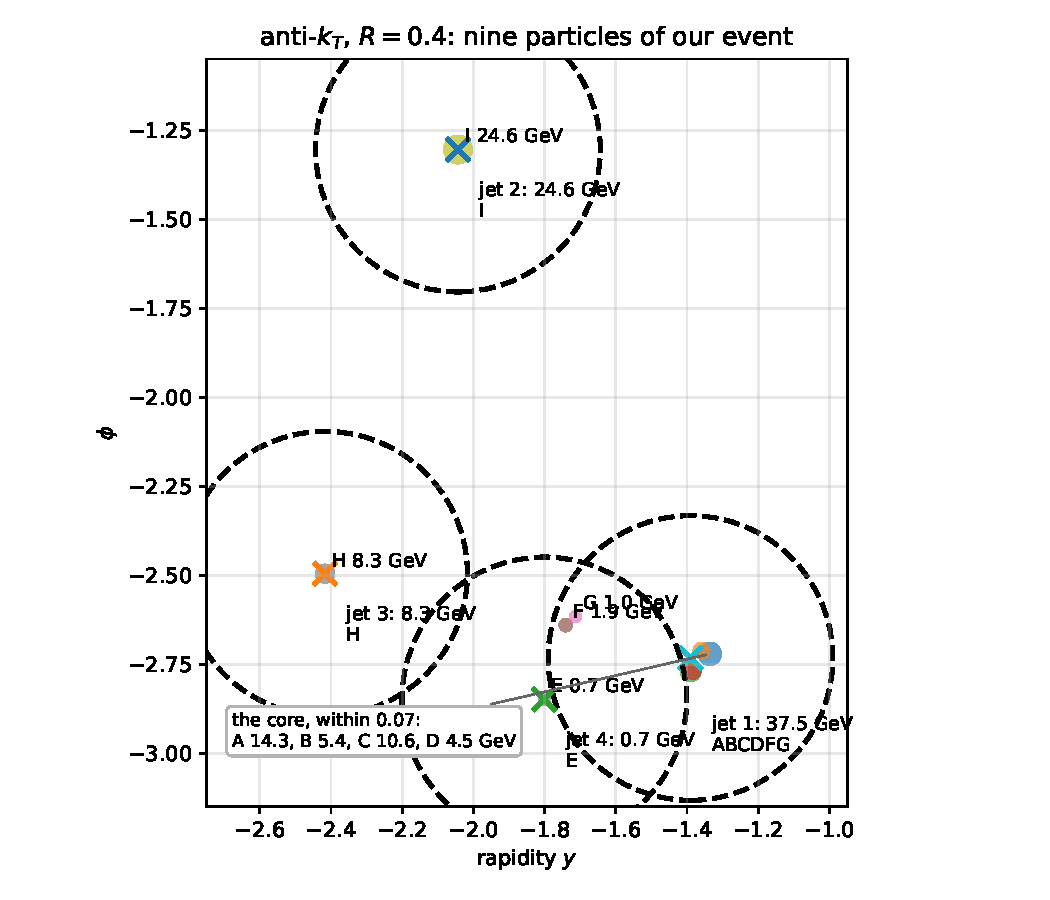
\includegraphics[width=0.46\textwidth]{GenJet/Standalone/antiKt.pdf}\hfill
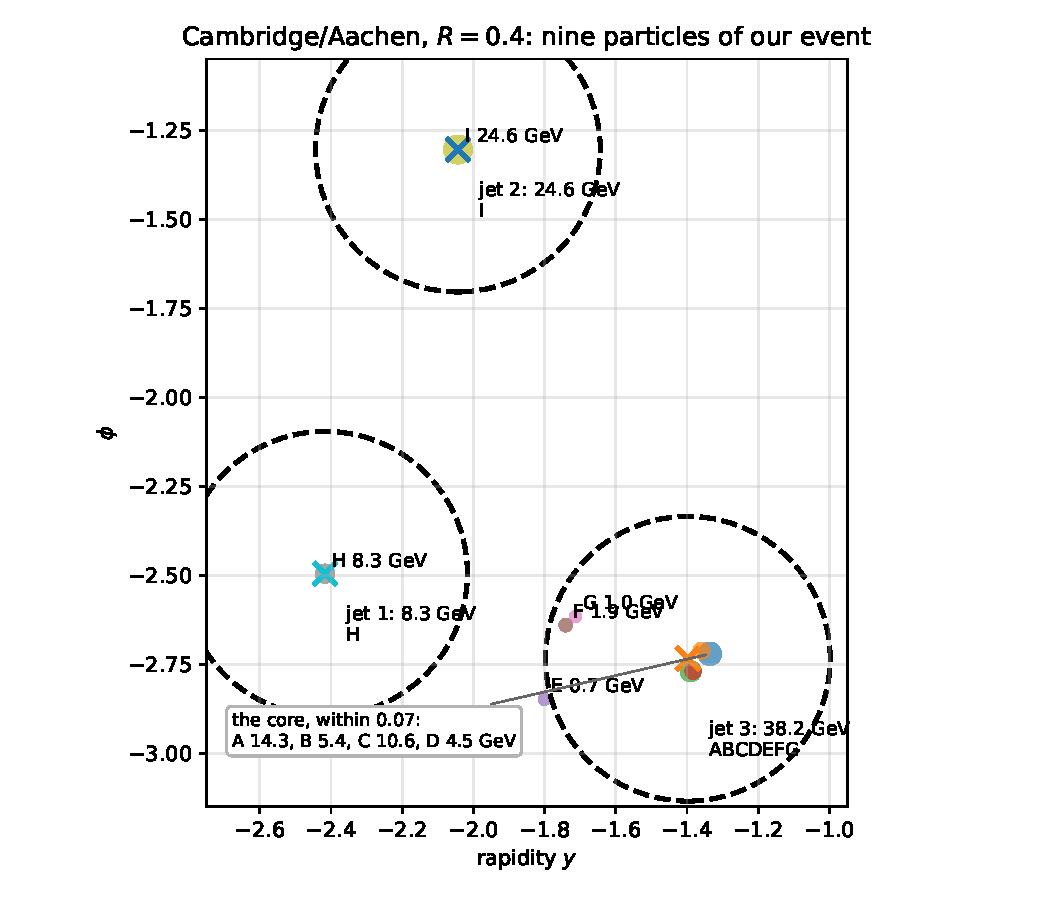
\includegraphics[width=0.46\textwidth]{GenJet/Standalone/caKt.pdf}\\[1mm]
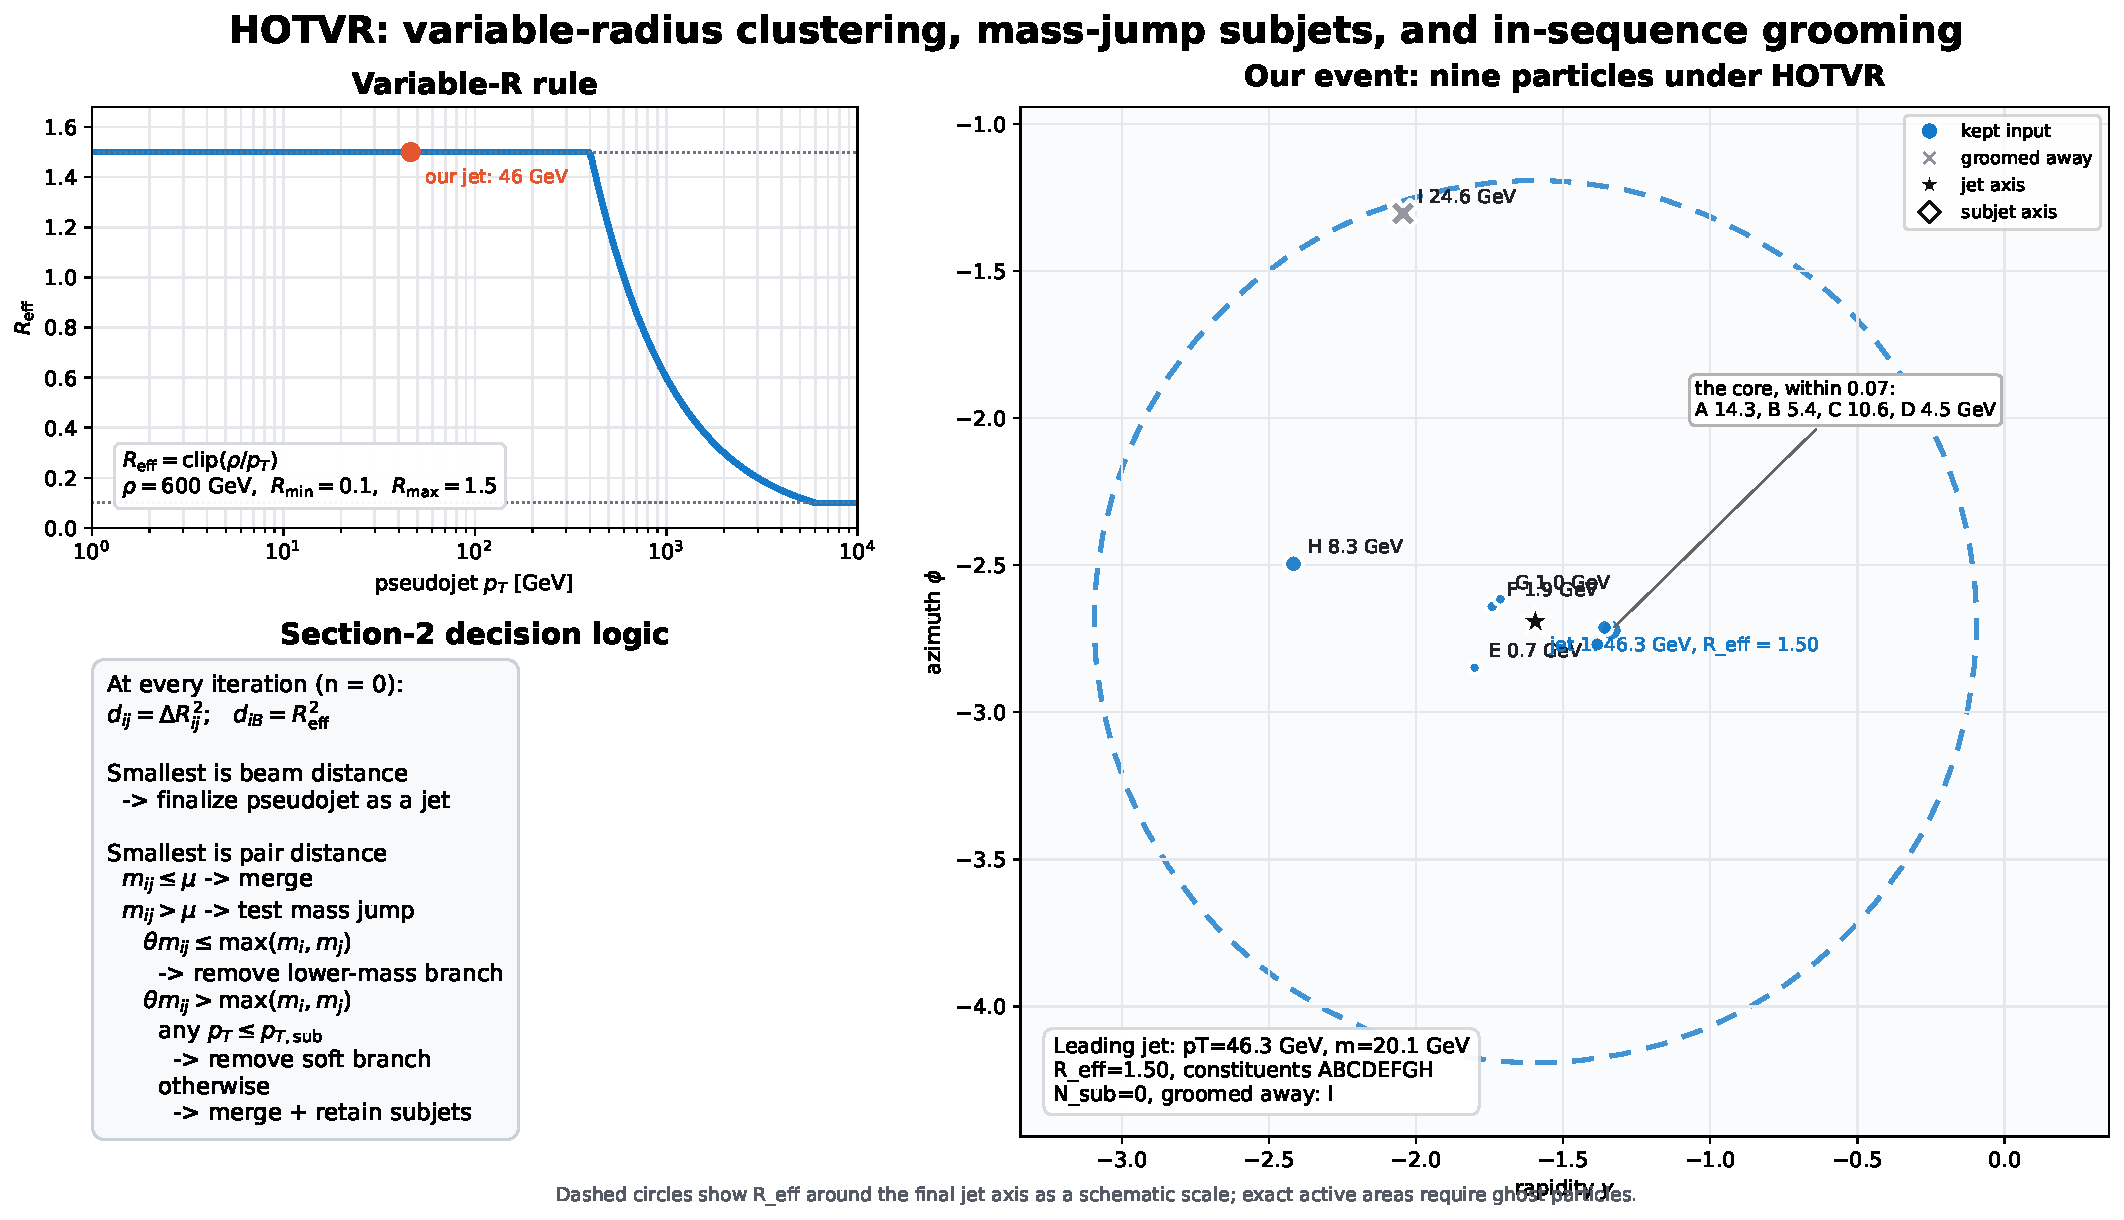
\includegraphics[width=0.9\textwidth]{GenJet/Standalone/hotVR.pdf}
\caption[The pictures drawn by the three scripts]{The pictures the three
scripts draw. Top: \antikt (left) and Cambridge/Aachen (right), a circle
of $R=0.4$ around every jet axis; E is a jet of its own on the left and a
constituent on the right. Bottom: \file{hotVR.py}, the variable-radius
rule, the decision logic of the paper's Section~2, and the nine particles
with their single HOTVR jet of $R_{\mathrm{eff}}=1.5$ and the groomed
pion.}
\label{fig:family_photograph:nine_pictures}
\end{figure}

\subsubsection{The photographer: \antikt and why the hard core comes first}
\label{sec:family_photograph:antikt}

Now the real jet. Thirty-one particles within $0.4$ of the mother, fifteen
of them the \Bbar's own; the nine of the previous section were four of
its core, three of its border and two neighbours, and the full family
gathers in the same order, the core first. If closest meant the smallest
angle, as it does for Cambridge/Aachen, the jet would grow from wherever
two soft particles happened to sit, a different place for every
fluctuation of the periphery. The distance of
\cref{eq:family_photograph:genkt} with $p=-1$,
\begin{equation}
  \dij=\min\!\big(p_{T,i}^{-2},\,p_{T,j}^{-2}\big)\,\frac{\dR_{ij}^2}{R^2}
      =\frac{1}{\max(p_{T,i},p_{T,j})^2}\,\frac{\dR_{ij}^2}{R^2},\qquad
  \diB=\frac{1}{p_{T,i}^2},
  \label{eq:family_photograph:dij}
\end{equation}
picks the \emph{harder} particle's inverse momentum. Between a particle of $15\GeV$ and one of $0.5$ at $\dR=0.3$ the
distance is $15^{-2}\times(0.3/0.4)^2=2.5\times10^{-3}$, and it would be
the same with the soft one at $3\GeV$ or at $0.05$: the soft particle's
momentum never enters. So every soft particle within $R$ of a hard one is
at a distance set by the hard one alone, all of them smaller than the
hard one's beam distance $15^{-2}=4.4\times10^{-3}$, and all of them
smaller than the distance between two soft particles, which carries the
inverse of a small momentum. The hard core therefore collects everything
within $R$ of itself before any soft pair elsewhere has a say, and only
then does its \diB win and the jet is declared: a circle of radius $R$
around the hard axis, moved by the soft periphery only through the
momentum it adds. That is why the photograph is round and why its axis
sits on the family, and it is the property, \emph{soft particles do not
change the jet's boundary}, that makes the picture stable against the
soft fluctuations of \cref{ch:uninvited_cousins} and against the crowd of
\cref{ch:crowd_on_the_road}. The \dR of
\cref{eq:family_photograph:dij} is in rapidity $y$ and not in
pseudorapidity, so that the distance is invariant under boosts along the
beam; for the massless particles of the periphery the two coincide, and
for a B~meson of half a GeV they do not, which is a trap of the last
section. The momenta are added as four-vectors, the \emph{E scheme}, so
that a jet has a mass, $14.8\GeV$ for ours, built from the opening angles
of its constituents.
\Cref{fig:family_photograph:distance_sketch} draws the distance and the
ladder of our event.

\begin{figure}[htbp]\centering
\resizebox{\textwidth}{!}{% ---------------------------------------------------------------------------
% How anti-kT takes the picture: (a) the distance d_ij = min(1/pT_i^2, 1/pT_j^2)
% dR^2/R^2 between a hard particle and a soft one is set by the hard one, so
% the hard core collects everything within R before anything else happens;
% (b) the ladder of our event's jet [0]: the 36 merges in order with their dR
% and the running pT (the -v log of standalone_genjets.py); (c) d_iB wins.
% ---------------------------------------------------------------------------
\begin{tikzpicture}[x=1cm,y=1cm,
  every node/.style={font=\footnotesize},
  lab/.style={font=\scriptsize,align=center},
  head/.style={font=\small\bfseries},
  hard/.style={circle,fill=red!75!black,inner sep=0pt,minimum size=7pt},
  soft/.style={circle,fill=black!45,inner sep=0pt,minimum size=3pt},
  dist/.style={-{Stealth[length=1.6mm]},black!60,thin},
  ring/.style={red!80!black,line width=1.2pt,dashed}]
% ---------------- (a) the distance ------------------------------------------------------------------
\begin{scope}
\node[head,anchor=west] at (-0.3,4.2) {(a) the hard one sets the distance};
\draw[ring] (1.6,1.4) circle (1.5);
\node[hard] (H) at (1.6,1.4) {};
\node[lab,text=red!80!black,anchor=south] at (1.6,1.65) {$i$: $p_T=15\,\mathrm{GeV}$};
\node[soft] (S1) at (2.5,2.2) {}; \node[soft] (S2) at (0.7,0.6) {}; \node[soft] (S3) at (2.2,0.4) {}; \node[soft] (S4) at (3.6,2.7) {};
\draw[dist] (H) -- (S1) node[midway,lab,above,sloped] {$\Delta R=0.3$};
\draw[dist] (H) -- (S2); \draw[dist] (H) -- (S3);
\draw[dist,dotted] (H) -- (S4) node[midway,lab,above,sloped] {$\Delta R=0.6$};
\node[lab,anchor=west] at (2.6,2.2) {$j$: $0.5\,\mathrm{GeV}$};
\node[lab,anchor=east] at (0.6,0.6) {$k$: $3\,\mathrm{GeV}$};
\node[lab,anchor=west] at (3.7,2.7) {$l$: outside $R$};
\node[lab,anchor=north west,text width=5.4cm,align=left] at (-0.3,-0.6) {$d_{ij}=\min\!\big(p_{T,i}^{-2},p_{T,j}^{-2}\big)\,\Delta R_{ij}^2/R^2
  =\dfrac{1}{15^2}\dfrac{0.3^2}{0.4^2}=2.5\times10^{-3}$\\[2pt]
  the same for $k$: the soft one's $p_T$ never enters; $d_{iB}=1/15^2=4.4\times10^{-3}$ is larger than every $d_{ij}$ inside $R$ and smaller than the one to $l$ ($10^{-2}$): $i$ collects $j$ and $k$, then becomes a jet without $l$};
\end{scope}
% ---------------- (b) the ladder of jet [0] ----------------------------------------------------------
\begin{scope}[xshift=7.4cm]
\node[head,anchor=west] at (-0.6,4.2) {(b) the 36 merges of our jet [0], in order};
\draw[-{Stealth}] (0,0) -- (6.3,0) node[below left,lab] {merge number};
\draw[-{Stealth}] (0,0) -- (0,3.8) node[left,lab] {$p_T$ of the pseudojet [GeV]};
\foreach \x/\t in {0.83/5,1.67/10,2.5/15,3.33/20,4.17/25,5.0/30,5.83/35} {\draw (\x,-0.05) -- (\x,0.05); \node[lab,anchor=north] at (\x,-0.08) {\t};}
\foreach \y/\t in {0.7/20,1.4/40,2.1/60,2.8/80,3.5/100} {\draw (-0.05,\y) -- (0.05,\y); \node[lab,anchor=east] at (-0.08,\y) {\t};}
% pT after each merge (from the -v log), scaled 0.035 cm per GeV, x = 0.1667 per merge
\draw[red!80!black,thick] plot[mark=*,mark size=0.9pt] coordinates {
 (0.167,0.526)(0.333,0.633)(0.5,0.633)(0.667,0.776)(0.833,0.776)(1.0,0.776)(1.167,0.815)(1.333,0.689)(1.5,1.003)(1.667,1.003)
 (1.833,1.123)(2.0,1.937)(2.167,2.040)(2.333,2.339)(2.5,2.490)(2.667,2.569)(2.833,2.687)(3.0,2.697)(3.167,2.750)(3.333,2.756)
 (3.5,2.768)(3.667,2.773)(3.833,2.794)(4.0,2.900)(4.167,3.056)(4.333,3.170)(4.5,3.234)(4.667,3.234)(4.833,3.300)(5.0,3.310)
 (5.167,3.346)(5.333,3.346)(5.5,3.380)(5.667,3.445)(5.833,3.470)(6.0,3.494)};
\node[lab,text=red!80!black,anchor=south west] at (3.4,3.55) {$99.83\,\mathrm{GeV}$, then $d_{iB}$ wins};
\node[lab,anchor=north west,text=black!65,text width=3.2cm,align=left] at (0.15,3.75) {the core: $K^-$, $\pi^-$, photons of the $\bar B^0$ at $\Delta R<0.04$};
\node[lab,anchor=south,text=black!65,text width=3.2cm,align=center] at (2.6,0.15) {merge 12 joins a second core, the $\pi^+\pi^-$ pair with the $K_S^0$, to the first};
\draw[dist] (4.6,1.2) -- (5.5,0.75);
\node[lab,anchor=east,text=black!65,text width=3.4cm,align=left] at (4.7,1.3) {the periphery: $0.1$ to $4.5\,\mathrm{GeV}$ each, at $\Delta R$ from $0.18$ to $0.38$};
\foreach \x in {0.5,0.833,1.0,1.667,4.667,5.333} {\draw[blue!60!black,thin] (\x,-0.02) -- (\x,0.12);}
\node[lab,text=blue!60!black,anchor=north] at (3.2,-0.45) {blue ticks: a ghost joins (merges 3, 5, 6, 10, 28, 32: $D^0$, $\bar B^0$, $b$, $D_s^-$, $g$, $g$)};
\end{scope}
% ---------------- (c) the rule in one line ------------------------------------------------------------
\begin{scope}[xshift=14.6cm]
\node[head,anchor=west] at (-0.4,4.2) {(c) when is it a jet?};
\node[lab,anchor=north west,text width=4.2cm,align=left] at (-0.4,3.7) {At every step the smallest of all $d_{ij}$ and $d_{iB}$ wins.\\[3pt]
 $d_{ij}$ smallest: $i+j\to k$, four-momenta added (E scheme), $k$ takes $i$'s and $j$'s place.\\[3pt]
 $d_{iB}$ smallest: $i$ is a jet; it is set aside.\\[3pt]
 For our jet: 36 merges, the last at $d_{ij}=9.2\times10^{-5}$, then $d_{iB}=1/99.83^2=1.0\times10^{-4}$.\\[3pt]
 Kept if $p_T>3\,\mathrm{GeV}$: 42 of the 928 pseudojets of the ak4 clustering (749 particles + 179 ghosts) end as jets above the threshold.};
\end{scope}
\end{tikzpicture}
}
\caption[The anti-$k_T$ distance, the ladder of our jet and the rule]{How
the picture is taken. Left: the distance of
\cref{eq:family_photograph:dij} with $p=-1$ between a hard particle and
its soft neighbours is set by the hard one, and the hard one's beam
distance is larger than every \dij inside $R$ and smaller than the one
to a particle outside. Middle: the 36 merges that built our \akfour jet,
in order, with the \pt of the pseudojet after each and the merges at
which a ghost joined. Right: the rule in one line.}
\label{fig:family_photograph:distance_sketch}
\end{figure}

\paragraph{The numbers.} The \code{-v} log lists the 36 merges of the
$b$ quark's jet in the order the event's 928 steps made them. The first,
step 12 of the whole event, is the hardest close pair of the family, the
$K^-$ ($s\bar u$) of $10.57\GeV$ and the $\pi^-$ of $4.45$ from the
$D^0$'s decay, at $\dR=0.006$ and $\dij=1.7\times10^{-6}$; a photon of
$3.06$ joins at $0.010$, another of $4.08$ at $0.020$, and by the seventh
merge the core has $23.3\GeV$. The ghosts arrive early, because they are
close: the $D^0$'s ghost at the third merge ($\dR=0.018$), the \Bbar's at
the fifth ($0.031$), the $b$ quark's at the sixth ($0.036$), each at a
distance set by the core's $18$ to $22\GeV$ and each adding nothing. The
twelfth merge joins a second core to the first, the $\pi^+\pi^-$ pair of
$19.7\GeV$ with the $K_S^0$ ($d\bar s$) of $9.0$, and the pseudojet jumps
from $32.1$ to $55.4\GeV$; the next seven merges add the kaon, pions and
photons of the \Bbar's remaining chain at $\dR$ from $0.08$ to $0.13$ and
bring it to $78.6$, the \Bbar's own momentum to within a few hundred MeV.
The last seventeen are the periphery, $0.1$ to $4.5\GeV$ each, from
$\dR=0.18$ to $0.38$, with the two gluon ghosts among them; the last
merge, a $\pi^+$ of $0.68\GeV$ at $0.381$, has $\dij=9.2\times10^{-5}$, and
then $\diB=1/99.83^2=1.0\times10^{-4}$ is the smallest distance the
pseudojet has left and it is a jet: $99.830\GeV$, $\eta=-1.439$,
$\phi=-2.712$, $m=14.83$, 31 particles, 17 of them charged. The cone of
$R=0.4$ around the quark holds $99.43\GeV$ in 31 particles too, but not
the same 31: the jet's axis is $0.062$ from the quark, and a $\pi^+$ of
$0.15\GeV$ and a photon of $0.26$ inside the cone are outside the jet,
while a $\pi^+$ of $0.68$ and a $\pi^-$ of $0.13$ inside the jet are
outside the cone, a net $+0.40\GeV$. Over four hundred decays the jet
exceeds the cone by $0.84\pm0.59\GeV$: the axis follows the family and the
cone does not. The $\bar b$'s jet, $94.09\GeV$ in 18 particles at
$\eta=-3.45$, exceeds its cone by $1.07$. Page~1 of
\file{theory_genjets.pdf} (\cref{fig:family_photograph:truejet_plot})
draws the ladder with the \dR of each merge.

\subsubsection{The whole event under the three rules, and why the experiments chose \antikt}
\label{sec:family_photograph:three_rules}

Nine particles show the rules; the event shows the consequences.
\file{plot_algorithms_GenJet.py} runs the three on the $749$ final
particles, \antikt and Cambridge/Aachen with the \code{Clustering} class
of the main script at $R=0.4$ and HOTVR with a NumPy copy of
\file{hotVR.py}'s decisions, checked against it on the nine, and draws
them side by side, \cref{fig:family_photograph:three_event}; the companion gives the
command and the HOTVR parameters.

\begin{figure}[htbp]\centering
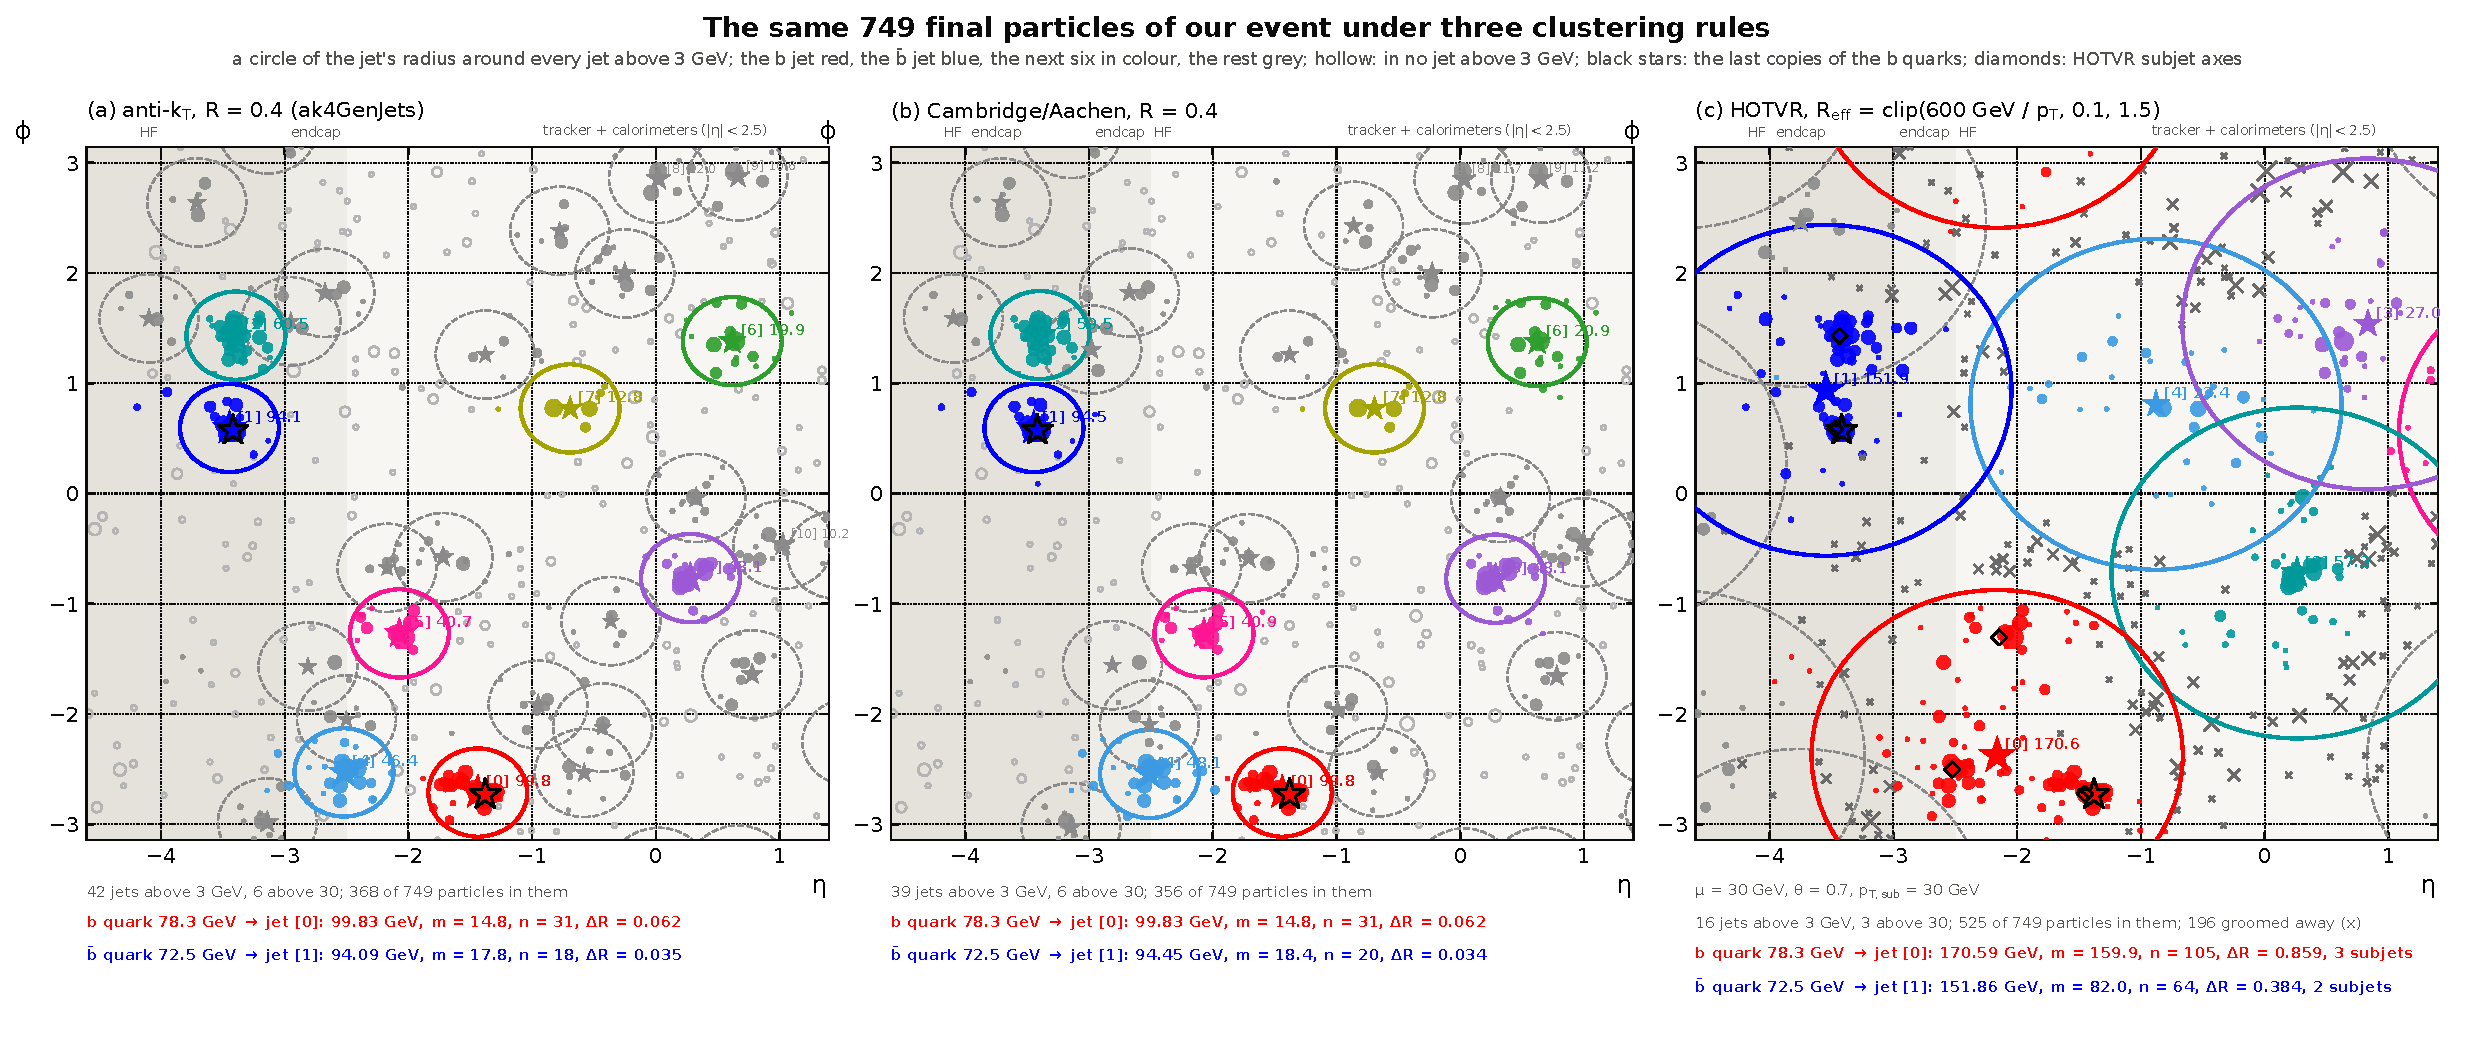
\includegraphics[width=\textwidth]{GenJet/Standalone/algorithms_genjets.pdf}
\caption[The same event under anti-$k_T$, Cambridge/Aachen and HOTVR]{The
same $749$ particles under the three rules, in the frame of
\cref{fig:family_photograph:journey}: a circle of the jet's radius
around every jet above $3\GeV$, the $b$ jet red, the $\bar b$ jet blue,
the next six in colour, the rest grey, particles in no jet hollow, the
particles HOTVR groomed away as crosses and its subjet axes as diamonds.
(a) \antikt, $R=0.4$: the \akfour of the record. (b) Cambridge/Aachen,
$R=0.4$. (c) HOTVR with the paper's parameters.}
\label{fig:family_photograph:three_event}
\end{figure}

\paragraph{The numbers.} \antikt makes $42$ jets above $3\GeV$ holding
$368$ particles, Cambridge/Aachen $39$ holding $356$, and the six hard
jets are the same six: our $b$ jet is the identical object under both,
$99.83\GeV$ in $31$ particles, because nothing soft sits on its border
with a soft neighbour outside. The $\bar b$ jet is not: $94.45\GeV$ in
$20$ particles under Cambridge/Aachen against $94.09$ in $18$, two soft
particles carried in as E was; the gluon jet [4] gains two as well,
$48.07$ in $27$ against $46.40$ in $25$, and jet [6] three. A third of a
GeV here, a GeV and a half there, each time from particles that have
nothing to do with the family, each time in a direction that depends on
where the soft periphery happened to be. HOTVR with the top-tagging
parameters takes a different photograph altogether: $16$ jets, $525$
particles in them and $196$ thrown away, the $b$ family inside a jet of
$170.59\GeV$, $105$ particles and a mass of $160\GeV$ whose three subjets
are \antikt's jets [0], [4] and [5], the $\bar b$ family inside one of
$151.86\GeV$ with [1] and [2] as its two subjets. It is the picture a top
quark would want, its three prongs in one circle with the soft dirt
removed; for two $b$ quarks it merges families that the matrix element
produced separately.

\paragraph{Why \antikt.} The experiments chose \antikt for their
standard jets in 2008~\cite{Cacciari:2008gp}, and the reason is in the
three panels. Its boundary is drawn by the hard core and does not move
when a soft particle is added, removed or shifted: so the underlying
event of \cref{ch:uninvited_cousins} and the pile-up of
\cref{ch:crowd_on_the_road} add momentum to a circle of known area
without redrawing it, which is what the subtraction of
\cref{ch:paying_for_uninvited} needs, and the detector's response to a
jet becomes a function of one radius, which is what the calibration of
\cref{ch:fair_price} needs. It is infrared and collinear safe like its two
siblings, so the cross section of a jet is a prediction of perturbative
QCD; and it is a sequential algorithm with the same $N\ln N$ bookkeeping,
so it costs nothing more~\cite{Cacciari:2011ma,Salam:2009jx}. What it
gives up, the angular ordering inside the jet, is recovered when it is
wanted: Cambridge/Aachen and $k_T$ recluster the constituents of an
\antikt jet to read its substructure, and HOTVR and its relatives are run
beside the standard collections for the boosted objects they were built
for. The photograph of the family is the \antikt one, and it stays so for
the rest of the journey.

\subsubsection{The choices: the radius, the neutrinos and the threshold}
\label{sec:family_photograph:choices}

Guess first: if the same family is photographed with $R=0.8$, how much
more does the picture hold, and is it still the same family? The \pt
inside a radius $R$ around the quark,
\begin{equation}
  \pt(R)=\Big|\sum_{\dR_i<R}\vec p_{T,i}\Big|,\qquad
  \pt^{\mathrm{jet}}(R)\simeq\pt(R)\ \text{for \antikt},
  \label{eq:family_photograph:ptR}
\end{equation}
is the family's profile, whose slope falls from the core outward and
rises again where the next jet begins. For ours it rises steeply to $78\GeV$ within
$R=0.15$, the \Bbar's descendants, flattens through $99.4$ at $0.4$ and
$108.7$ at $0.8$ as the gluons' hadrons and the underlying event of
\cref{ch:uninvited_cousins} are added at a few GeV per tenth of a unit,
and jumps to $160$ beyond $R=1$, where the gluon jet [4] of $46\GeV$ at
$\dR=1.1$ is swallowed whole. The \antikt jets follow the profile to
within a GeV, $99.83$ at $0.4$ and $105.79$ at $0.8$, the second a little
below its cone because the \akeight axis has moved towards the gluon's
family. What the radius chooses is therefore where on that profile the
photograph is cut: at $0.4$ the family and little else, at $0.8$ the
family with its wide-angle radiation and twice the underlying event,
$47$ particles instead of $31$ and a mass of $27\GeV$ instead of $15$.
The second choice is who may be in the picture. \CMSSW's
\code{genParticlesForJets} takes every stable particle but a list of
invisibles that do not occur here, neutralinos and gravitinos, and
\code{genParticlesForJetsNoNu} removes the neutrinos as well; the jets of
the first are \akfour and \akeight, the jets of the second \akfournonu,
and the second is what CMS calibrates its reconstructed jets
to~\cite{CMS:2016lmd}, because the detector cannot see a neutrino and a
correction that asked it to would push every $b$ jet up by the average
neutrino and smear it by the spread. In our event the \Bbar decayed
hadronically and the two \akfour collections are the same jet; in
decay seed~4 of the same hadrons the B went semileptonic and the jet
without neutrinos has $90.2\GeV$ instead of $99.6$; over four hundred
decays the jet with neutrinos is $99.63\pm0.49\GeV$ and the jet without
them $91.93\pm12.12$, no neutrino in $54\%$ of the decays and more than
$5\GeV$ of them in $37\%$; the \CMSSW event lost $38\GeV$ this way. The
third choice is the threshold. \antikt declares every pseudojet a jet,
down to a single soft particle alone in its circle, and
\code{GenJetParameters.jetPtMin} $=3\GeV$ is where \CMSSW stops writing
them: $42$ \akfour jets in our event, $11$ above $10\GeV$ and $6$ above
$30$, the two $b$ jets and four gluon and quark jets from the shower and
the secondary scatterings of \cref{ch:uninvited_cousins}. The $30\GeV$
of an analysis is a fourth choice made later, in
\cref{ch:paying_for_uninvited}, and the number of jets a photograph holds
depends on it more than on anything in this chapter.

\paragraph{The numbers.} Page~1 of \file{theory_genjets.pdf}
(\cref{fig:family_photograph:truejet_plot}) has the three: the profile of
\cref{eq:family_photograph:ptR} for the cone and the jet, with and without
the neutrinos, from $R=0.1$ to $1.2$; the ladder; and the number of jets
above a threshold from $0$ to $60\GeV$, $42$, $11$, $6$, $3$ at $3$, $10$,
$30$ and $50$. The \akeight collection has $30$ jets holding $600$ of the
$749$ particles, $16$ above $10\GeV$ and $5$ above $30$: fewer jets above
the threshold than \akfour although each is larger, because two of the
six hard \akfour jets, the $\bar b$'s and the gluon pair's, are one
\akeight jet of $147.69\GeV$ at $\dR=0.36$ from the $\bar b$ quark, with
$57$ particles and a mass of $75\GeV$. The \CMSSW event, with its $634$
particles, has $27$ \akfour jets and $28$ \akeight jets.

\begin{figure}[htbp]\centering
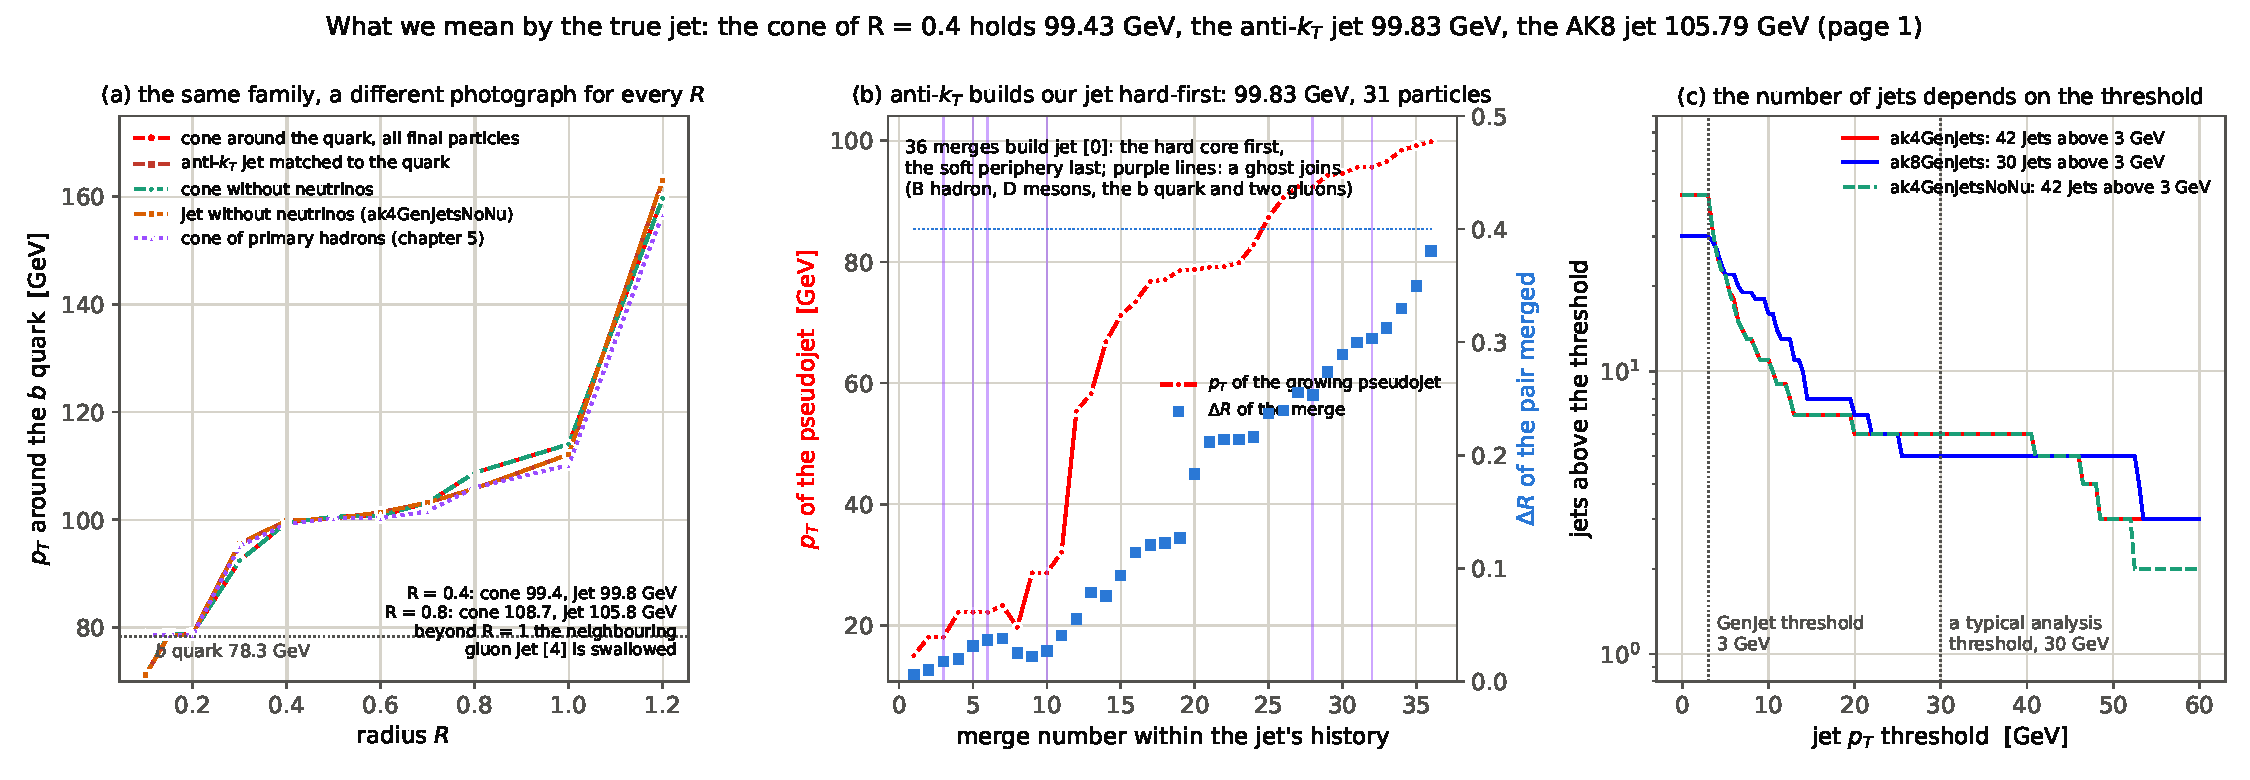
\includegraphics[page=1,width=\textwidth]{GenJet/Standalone/theory_genjets.pdf}
\caption[The profile against the radius, the ladder of our jet and the
threshold]{Page~1 of \file{theory_genjets.pdf}. (a) The \pt within $R$ of
the $b$ quark, \cref{eq:family_photograph:ptR}, for the cone of final
particles and the matched \antikt jet, with and without the neutrinos,
and for the primary hadrons of \cref{ch:children_getting_married}, from
$R=0.1$ to $1.2$. (b) The 36 merges of our \akfour jet in order, the \pt
of the pseudojet after each and the \dR of each merge, with the merges at
which a ghost joined marked. (c) The number of jets above a \pt threshold
for the three collections.}
\label{fig:family_photograph:truejet_plot}
\end{figure}

\subsection{Ghost-associated hadron flavour vs parton flavour}
\label{sec:family_photograph:ghost_associated_hadron_flavour_vs_parto}

The picture is taken; now the label.

\subsubsection{The ghosts and the \CMSSW labels}
\label{sec:family_photograph:ghosts}

Guess first: the \Bbar decayed $21\mm$ from the vertex and is nowhere
among the 749 particles. How does the experiment decide that jet [0] is a
$b$ jet and jet [3] is not? It could follow the record backwards from
every constituent, but the record of a \PYTHIA event is a tangle of
copies and the record of real data does not exist; the method has to be
one that works on the jet alone. \CMSSW's \code{JetFlavourClustering}
puts the hadron back as a \emph{ghost}: it takes the last $b$ hadron of
every decay chain, the last $c$ hadron, the partons that were handed to
the strings and the leptons from heavy-hadron decays, rescales each
four-momentum by
\begin{equation}
  p^\mu\to\varepsilon\,p^\mu,\quad\varepsilon=10^{-18},\quad
  d_{\mathrm{ghost},j}=\min\!\big((\varepsilon p_T)^{-2},p_{T,j}^{-2}\big)\frac{\dR^2}{R^2}=\frac{\dR^2}{p_{T,j}^{2}R^2},\quad
  d_{\mathrm{ghost},B}=\frac{10^{36}}{p_T^2},
  \label{eq:family_photograph:ghost}
\end{equation}
and clusters again with the ghosts among the particles. The second and
third members of \cref{eq:family_photograph:ghost} say why this works: the
distance between a ghost and any real pseudojet is the real one's, so the
ghost is filed under whatever hard pseudojet is within $R$ of it, exactly
as a soft particle would be, and its beam distance is so large that it
can never become a jet of its own; its momentum changes the jet it joins
by one part in $10^{18}$, below the precision of a double. The jet that
catches the ghost of a $b$ hadron is a $b$ jet. The labels are then two
integers per jet:
\begin{equation}
\begin{aligned}
  \hadflav&=\begin{cases}5 & \text{a $b$-hadron ghost in the jet,}\\ 4 & \text{else a $c$-hadron ghost,}\\ 0 & \text{else,}\end{cases}\\[4pt]
  \partflav&=\begin{cases}\pm5 & \text{the id of the hardest $b$-parton ghost,}\\ \pm4 & \text{else of the hardest $c$,}\\ 21,\pm1,\pm2,\pm3 & \text{else of the hardest parton,}\\ 0 & \text{none,}\end{cases}
\end{aligned}
  \label{eq:family_photograph:labels}
\end{equation}
the first unsigned and from the hadrons, the second signed and from the
partons of status 71 to 79, \PYTHIA's copies of the final partons as they
enter the hadronisation, which the standalone record carries as the rows
the strings were built from. The hadron label is what the $b$-tagging
efficiencies of \cref{ch:footprints} are measured
against~\cite{CMS:2017wtu}; the parton label is what a gluon jet and a
quark jet are told apart by in a calibration, and the two disagree
whenever a gluon splits into a heavy pair, which is a quarter of all
$b$-labelled jets in a QCD sample. Two older definitions are kept for
comparison. The \emph{physics definition} uses the hard-process partons,
status 23, as the ghosts, and the Run-1 matching took the hardest parton
within $\dR<0.3$ of the axis; both ask the hard process rather than the
hadrons, and \cref{fig:family_photograph:ghosts_sketch} shows what
happens to them in our event.

\begin{figure}[htbp]\centering
\resizebox{\textwidth}{!}{% ---------------------------------------------------------------------------
% Ghost association: (a) the Bbar0 has decayed; it is put back with its
% momentum times 1e-18, follows the clustering and lands in the jet without
% moving it; (b) the labels of CMSSW's JetFlavourClustering for the three
% b jets of our event; (c) why the physics definition (the status-23 quark)
% fails for the AK4 jet: ISR moved the hard system and the shower the family.
% Numbers: event_GenJet.lhe and standalone_genjets.log (seed 1).
% ---------------------------------------------------------------------------
\begin{tikzpicture}[x=1cm,y=1cm,
  every node/.style={font=\footnotesize},
  lab/.style={font=\scriptsize,align=center},
  head/.style={font=\small\bfseries},
  fam/.style={circle,fill=red!75!black,inner sep=0pt},
  oth/.style={circle,fill=black!40,inner sep=0pt},
  ring/.style={red!80!black,line width=1.4pt},
  ghost/.style={star,star points=5,draw=red!80!black,fill=white,thick,inner sep=1.4pt},
  flow/.style={-{Stealth[length=2mm]},thick},
  tbl/.style={font=\scriptsize,inner sep=2pt}]
% ---------------- (a) the ghost -------------------------------------------------------------------
\begin{scope}
\node[head,anchor=west] at (-0.4,4.3) {(a) the hadron comes back as a ghost};
% before: the B hadron as a particle
\node[lab,anchor=west] at (-0.4,3.7) {before the decays: the $\bar B^0$ is a particle of $78.3\,\mathrm{GeV}$};
\node[fam,minimum size=9pt] (B) at (1.2,2.9) {};
\node[lab,text=red!80!black,anchor=west] at (1.4,2.9) {$\bar B^0$ ($b\bar d$), row 1527};
\draw[flow] (1.2,2.5) -- (1.2,1.6) node[midway,right,lab] {decays: $D_s^{*-}D^{*0}\rho^+$, 15 final particles};
% after: the descendants and the ghost
\draw[ring] (1.2,0.2) circle (1.25);
\foreach \p/\s in {(1.25,0.3)/5,(1.1,0.1)/4,(1.35,0.05)/3.5,(1.0,0.45)/3,(1.5,0.4)/2.6,(0.85,-0.1)/2.4,(1.6,-0.2)/2.2,(0.7,0.55)/2,(1.3,0.75)/1.8,(0.6,-0.45)/1.6,(1.85,0.6)/1.5,(1.15,-0.6)/1.4,(1.95,-0.5)/1.3,(0.35,0.1)/1.2,(1.7,0.95)/1.1} {\node[fam,minimum size=\s pt] at \p {};}
\foreach \p/\s in {(0.5,0.95)/1.6,(2.05,0.1)/1.4,(0.3,-0.7)/1.3,(1.9,-0.95)/1.2,(0.9,1.1)/1.1,(2.2,0.8)/1.0} {\node[oth,minimum size=\s pt] at \p {};}
\node[ghost] at (1.2,0.2) {};
\draw[flow,red!80!black] (3.2,2.9) -- (3.2,1.9) node[midway,right,lab,text=red!80!black] {$p\to10^{-18}\,p$};
\node[lab,text=red!80!black,anchor=west,text width=3.3cm,align=left] at (2.6,0.3) {the ghost: same direction, no momentum; $d_{ij}=p_{T,j}^{-2}\Delta R^2/R^2$ with any real $j$, so anti-$k_T$ files it under the nearest hard pseudojet within $R$; $d_{iB}=10^{36}/p_T^2$ never wins};
\node[lab,anchor=north west,text width=5.8cm,align=left,text=black!65] at (-0.4,-1.3) {In our event the $\bar B^0$'s ghost joins the pseudojet at the fifth of its 36 merges (step 24 of the event), $\Delta R=0.031$ from the running axis, between a photon and the $b$ quark's own ghost; the jet momentum changes by one part in $10^{18}$, below double precision.};
\end{scope}
% ---------------- (b) the labels ------------------------------------------------------------------
\begin{scope}[xshift=7.6cm]
\node[head,anchor=west] at (-0.4,4.3) {(b) the labels of the three $b$ jets (ak4)};
\foreach \x/\t in {0.1/jet,1.0/ghosts clustered} {\node[tbl,font=\scriptsize\bfseries,anchor=west] at (\x,3.6) {\t};}
\foreach \x/\t in {4.6/hadron,5.6/parton,6.6/physics,7.7/$\Delta R<0.3$,8.6/net} {\node[tbl,font=\tiny\bfseries] at (\x,3.6) {\t};}
\foreach \y/\j/\g/\h/\p/\f/\d/\n in {3.15/{[0] $99.8$}/{$\bar B^0$, $D^0$, $D_s^-$; $b$, $g$, $g$}/5/$+5$/0/$+5$/$+1\,b$,
                                     2.7/{[1] $94.1$}/{$\bar B^0$ (osc.), $\Xi_c^0$; $\bar b$, $g$, $g$, $g$}/5/$-5$/0/$-5$/$+1\,b$,
                                     2.25/{[2] $60.5$}/{$\bar B^0$, $\bar\Lambda_b^0$, $D^+$, $\bar D^0$; $\bar b$, $b$, $g$}/5/$-5$/0/$-5$/$0$} {
  \node[tbl,anchor=west] at (0.1,\y) {\j};
  \node[tbl,anchor=west,font=\tiny] at (1.0,\y) {\g};
  \node[tbl,fill=red!15] at (4.6,\y) {\h};
  \node[tbl] at (5.6,\y) {\p};
  \node[tbl,fill=black!8] at (6.6,\y) {\f};
  \node[tbl] at (7.7,\y) {\d};
  \node[tbl] at (8.6,\y) {\n};}
\node[lab,anchor=north west,text width=7.6cm,align=left] at (-0.4,1.55) {\textbf{hadronFlavour}: 5 if a $b$-hadron ghost is in the jet, else 4 for a $c$ hadron, else 0.\\[2pt]
 \textbf{partonFlavour}: the id of the hardest $b$-parton ghost (status 71--79), else the hardest $c$, else the hardest parton: $+5$, $-5$, or $21$, $\pm1$, $\pm2$, $\pm3$.\\[2pt]
 \textbf{physics}: the same rule with the status-23 partons as ghosts.\\[2pt]
 \textbf{net}: the sum of $\pm1$ over the $b$ hadrons, $+1$ for a $b$ quark inside ($\bar B^0$, $\Lambda_b^0$), $-1$ for a $\bar b$ ($B^0$, $B^+$, $\bar\Lambda_b^0$).};
\node[lab,anchor=north west,text width=7.6cm,align=left,text=black!65] at (-0.4,-2.4) {Jet [1] reads $+1\,b$ although it is the $\bar b$ quark's: its $B^0$ oscillated. Jet [2] holds the gluon's pair, $b$ and $\bar b$: hadronFlavour 5, net 0.};
\end{scope}
% ---------------- (c) the physics definition fails ------------------------------------------------
\begin{scope}[yshift=-8.6cm]
\node[head,anchor=west] at (-0.4,4.3) {(c) where the status-23 quark points};
\draw[ring] (1.0,1.0) circle (1.2);
\node[star,star points=5,fill=red!80!black,inner sep=1.2pt] at (1.0,1.0) {};
\node[lab,text=red!80!black,anchor=north] at (1.0,0.8) {jet [0]\\ $(-1.44,-2.71)$};
\node[star,star points=5,draw=black,fill=white,inner sep=1.3pt] at (0.75,0.95) {};
\node[lab,anchor=south east] at (0.7,1.1) {$b$, status 62\\ $(-1.38,-2.73)$};
\draw[green!50!black,thick] (0.88,2.56) -- (1.12,2.80) (0.88,2.80) -- (1.12,2.56);
\node[lab,text=green!50!black,anchor=west] at (1.15,2.75) {$b$, status 23\\ $(-1.44,-2.15)$: $\Delta R=0.56$};
\draw[black!60,thin,-{Stealth[length=1.6mm]}] (1.0,2.5) -- (1.0,1.2);
\node[lab,anchor=north west,text width=9.6cm,align=left] at (4.4,3.8) {\textbf{The physics definition asks the hard process, not the hadrons.} The status-23 $b$ quark of the matrix element points $0.56$ from the axis of jet [0] and is caught only by the AK8 jet, whose radius reaches it. What moved: ISR gave the hard system a recoil (\cref{ch:mother_gives_birth}), and the shower that followed, the two gluon emissions of the $b$ and the recoils of the dipoles, carried the family to $(-1.38,-2.73)$, where the last copy of the quark (status 62) and the $\bar B^0$ sit. The ghost of the last copy is in the jet; the ghost of the first is not.\\[3pt]
 The CMS ``physics definition'' of Run~1 matched the status-3 parton within $\Delta R<0.3$ of the axis and would have found nothing here either: physics flavour 0 for a jet that holds the $b$ quark's whole family. That is why \CMSSW's labels of choice are the hadron and the parton flavour, read from the ghosts of the \emph{last} copies.};
\node[lab,anchor=north west,text width=4.6cm,align=left,text=black!65] at (-0.4,-0.5) {red: AK4 jet [0], $R=0.4$; white star: the last $b$ quark; green cross: the status-23 $b$; $\Delta R$ in $(\eta,\phi)$.};
\end{scope}
\end{tikzpicture}
}
\caption[The ghost, the labels of the three $b$ jets and the physics
definition]{The ghosts. Top left: the \Bbar has decayed; it is put back
with its momentum times $10^{-18}$, \cref{eq:family_photograph:ghost},
follows the clustering and lands in the jet without moving it. Top right:
the labels of \cref{eq:family_photograph:labels} for the three
$b$-flavoured \akfour jets of our event, with the ghosts behind each.
Bottom: where the status-23 $b$ quark points, $0.56$ from the jet, and
why.}
\label{fig:family_photograph:ghosts_sketch}
\end{figure}

\paragraph{The numbers.} The log lists the ghosts: four $b$ hadrons, the
\Bbar of the mother at $78.26\GeV$, the oscillated \Bbar of the $\bar b$
at $81.97$, and the gluon's pair of \cref{ch:mother_gives_birth}, a
\Lbbar ($\bar u\bar d\bar b$) of $35.5$ and a \Bbar of $24.9$, both at
$\eta=-3.4$; nine $c$ hadrons, from a $D^+$ of $0.1\GeV$ to the
$\Xi_c^0$ ($dsc$) of $71.4$; $161$ partons of status 71 to 79; the two
status-23 quarks; and three leptons, $179$ ghosts in all, so that the
\akfour clustering has $928$ pseudojets to start from. Jet [0] catches
the \Bbar's ghost at its fifth merge, the $D^0$'s and the $D_s^-$'s, the
$b$ quark's and two gluons': $\hadflav=5$, $\partflav=+5$, the $\dR<0.3$
label $+5$, and the physics label $0$, because the status-23 $b$ quark
sits at $(\eta,\phi)=(-1.44,-2.15)$, $0.56$ from the jet's axis at
$(-1.44,-2.71)$. The reason is two stops back: the initial-state
radiation of \cref{ch:mother_gives_birth} recoiled the hard system and
the final-state shower moved the quark from its hard-process direction,
so that the last copy of the quark, at $(-1.38,-2.73)$, and everything
descended from it are half a unit from where the hard process put them.
The physics definition would have found this $b$ jet only with $R=0.8$,
where the status-23 ghost is inside and the label is $+5$. Jet [1], the
$\bar b$'s, has $\hadflav=5$ and $\partflav=-5$; its net flavour, the
sum of $\pm1$ over its $b$ hadrons, reads $+1$ although it is the $\bar b$
quark's jet, because the \Bz oscillated in
\cref{sec:children_producing_grandchildren:mixing} and the record holds
the \Bbar it decayed as. Jet [2], $60.45\GeV$ next to it, holds the
gluon's pair, \Lbbar and \Bbar, a $\bar b$ and a $b$: $\hadflav=5$,
$\partflav=-5$ from the harder of the two parton ghosts, net flavour
$0$. The \akeight jet of the $\bar b$ holds all three, and its physics
label is $-5$. Over four hundred decays the \Bbar's ghost lands in the
mother's \akfour jet every time, $0.062$ from the axis, with $0.20$ of its
descendants outside the jet on average and $78.2\pm0.5\%$ of the jet's
\pt from them; \hadflav is $5$ and \partflav $+5$ in $100\%$ of the
decays, and the \PYTHIA chain with \FASTJET gives $99.2$ and $99.3\%$, the
rest being decays in which the shower moved the family further than the
jet's radius. The net flavour of the mother's jet is $+1$ in $83.2\%$ and
$-1$ in $16.8\%$: the oscillation rate of
\cref{sec:children_producing_grandchildren:mixing}, read off a jet label.
Page~2 of \file{theory_genjets.pdf} (\cref{fig:family_photograph:flavour_plot})
draws the ghosts over the jets, the six labels of every jet above
$5\GeV$, and the ensemble.

\begin{figure}[htbp]\centering
\includegraphics[page=2,width=\textwidth]{GenJet/Standalone/theory_genjets.pdf}
\caption[The ghosts over the jets, the six labels of every jet, and the B
hadron against the axis]{Page~2 of \file{theory_genjets.pdf}. (a) The
ghosts of our event, $b$ hadrons, $c$ hadrons, the status-23 partons and
the status-71 partons above $3\GeV$, over the \akfour jets of the two $b$
regions. (b) One jet, six labels: \hadflav, \partflav, the physics and
the $\dR<0.3$ definitions, and the net and IFN $b$ flavours with the
heavy hadrons kept, for the 22 \akfour jets above $5\GeV$. (c) Over four
hundred decays, the \dR between the \Bbar and the axis of the mother's
jet and the share of the jet's \pt that its descendants carry.}
\label{fig:family_photograph:flavour_plot}
\end{figure}

\subsection{Infrared-safe flavour: flavour-$k_T$ and interleaved flavour neutralisation}
\label{sec:family_photograph:infrared_safe_flavour_flavour_k_t_and_in}

Guess first: a gluon in the periphery of the event splits into a $b\bar b$
pair so soft, half a GeV of \pt each, that it should change nothing, and
its two B~mesons land one in jet [8] and one in jet [9], two light jets of
$12$ and $11\GeV$. What are the labels now? Under
\cref{eq:family_photograph:labels} both jets have become $b$ jets, and
under the net flavour one is $+1$ and the other $-1$. A splitting of
vanishing momentum has changed two labels, and that is the definition of
an infrared-unsafe quantity~\cite{Sterman:1977wj,Salam:2009jx}: in a
perturbative calculation the soft $g\to b\bar b$ splitting comes with a
logarithm of the pair's mass over the jet's \pt that diverges as the pair
becomes soft, and a quantity that sees the pair inherits the divergence.
The jet's momentum does not, which is the point of \antikt; the jet's
flavour does. For the experiment, whose labels are applied to a
simulation with a finite cut-off, this is a definition and not a
disaster, and \hadflav is what the taggers are calibrated against; for a
comparison with a calculation beyond leading order, and for the $Z+b$,
$W+c$ and $t\bar t+b\bar b$ measurements that need
one~\cite{Banfi:2007gu,Gauld:2020deh}, a safe definition is needed, and
the literature has three. Flavour-$k_T$~\cite{Banfi:2006hf} changes the
distance so that a soft flavoured particle is pulled to its partner
before it can join a jet,
\begin{equation}
  \dij^{(F)}=\frac{\dR_{ij}^2}{R^2}\times\begin{cases}
    \max(k_{T,i},k_{T,j})^{\alpha}\,\min(k_{T,i},k_{T,j})^{2-\alpha} & \text{the softer of $i,j$ is flavoured,}\\
    \min(k_{T,i},k_{T,j})^2 & \text{otherwise,}\end{cases}
  \label{eq:family_photograph:fkt}
\end{equation}
with $\alpha=1$ or $2$, and the same for the beam distances with a beam
``momentum'' $k_{T,B}(y_i)=\sum_j k_{T,j}[\Theta(y_j-y_i)+\Theta(y_i-y_j)e^{y_j-y_i}]$
that sums the event on either side of the particle in rapidity: a soft
$b$ near a hard jet is as far from the jet as the jet is hard, and as
close to its soft $\bar b$ as their angle. The price is that the jets are
$k_T$ jets, irregular and different from the experiment's, which is why
it was never used on data. Flavour anti-$k_T$~\cite{Czakon:2022khx} and
flavour dressing~\cite{Gauld:2022lem} keep the \antikt jets and modify
either the distance when both are flavoured or the assignment
afterwards. Interleaved flavour neutralisation~\cite{Caletti:2022glq}
keeps the \antikt clustering exactly and adds a step before every
recombination of a flavoured pseudojet: with the neutralisation distance
\begin{equation}
  \uik=\max(p_{T,i},p_{T,k})^{\alpha}\min(p_{T,i},p_{T,k})^{2-\alpha}\,\Omega_{ik}^2,\qquad
  \Omega_{ik}^2=2\Big[\frac{\cosh(\omega\Delta y_{ik})-1}{\omega^2}-(\cos\Delta\phi_{ik}-1)\Big],
  \label{eq:family_photograph:ifn}
\end{equation}
$\alpha=2$ and $\omega=1$ for \antikt, the flavour of $i$, about to be
merged with $j$, is cancelled against every pseudojet $k$ of opposite
flavour with $\uik<u_{ij}$, closest first, each candidate's own closer
partners being settled before it; then $i$ and $j$ are merged as \antikt
would have merged them. With $\alpha=2$ the distance between the soft
$b$ and the hard core it is about to join is the core's $p_T^2$ times
their angle, and the distance between the soft $b$ and its soft $\bar b$
is their own small $p_T^2$ times their angle: the pair cancels first,
unless it is hard enough that $p_T^2\Omega^2$ of the pair exceeds that of
the merge, at which point it is a real $b\bar b$ and keeps its flavour.
$\Omega^2$ is $\dR^2$ at small angles and grows like $e^{|\Delta y|}$ at
large rapidity separation, so that a flavour far down the beam cannot
neutralise one in the barrel. The jets are the \antikt jets to the last
digit; only the labels change. The script runs
\cref{eq:family_photograph:fkt,eq:family_photograph:ifn} on the record
with the heavy hadrons kept undecayed, as the hadron-level tests of the
papers do, since a decayed B has no flavour to carry.
\Cref{fig:family_photograph:irsafety_sketch} draws the whisper and the
neutralisation.

\begin{figure}[htbp]\centering
\resizebox{\textwidth}{!}{% ---------------------------------------------------------------------------
% Infrared-safe flavour: (a) a soft g -> b bbar pair between two light jets
% relabels both under the ghost and the net definitions; (b) IFN: before the
% soft B joins its jet, its flavour is neutralised against the nearer
% opposite flavour in the distance u_ik; (c) the three distances side by
% side. Numbers: standalone_genjets.py --soft-pair 0.5 (jets [8] and [9]).
% ---------------------------------------------------------------------------
\begin{tikzpicture}[x=1cm,y=1cm,
  every node/.style={font=\footnotesize},
  lab/.style={font=\scriptsize,align=center},
  head/.style={font=\small\bfseries},
  oth/.style={circle,fill=black!40,inner sep=0pt},
  ring/.style={black!55,line width=1.2pt},
  bq/.style={star,star points=5,fill=red!80!black,inner sep=1.4pt},
  bbq/.style={star,star points=5,fill=blue!70!black,inner sep=1.4pt},
  glu/.style={decorate,decoration={coil,aspect=0.6,segment length=1.4mm,amplitude=0.7mm},green!50!black,thick},
  neut/.style={green!50!black,line width=2pt},
  box/.style={draw,rounded corners=3pt,thin,fill=gray!6,align=left,inner sep=4pt,text width=6.6cm,font=\scriptsize}]
% ---------------- (a) the whisper -------------------------------------------------------------------
\begin{scope}
\node[head,anchor=west] at (-0.4,4.3) {(a) a whisper relabels two jets};
\draw[ring] (1.0,1.2) circle (1.2); \draw[ring] (3.4,1.3) circle (1.2);
\foreach \p/\s in {(1.0,1.25)/4.5,(0.8,1.0)/3,(1.3,1.4)/2.6,(0.6,1.5)/2,(1.2,0.7)/1.8,(1.5,1.0)/1.5,(0.4,0.9)/1.3} {\node[oth,minimum size=\s pt] at \p {};}
\foreach \p/\s in {(3.4,1.35)/4.2,(3.6,1.1)/2.8,(3.15,1.6)/2.4,(3.8,1.6)/1.9,(3.2,0.8)/1.6,(3.9,1.0)/1.4,(3.5,1.9)/1.2} {\node[oth,minimum size=\s pt] at \p {};}
\node[lab,anchor=south] at (1.0,2.45) {jet [9], $10.6\,\mathrm{GeV}$};
\node[lab,anchor=south] at (3.4,2.55) {jet [8], $12.0\,\mathrm{GeV}$};
% the gluon splitting between them
\draw[glu] (2.2,-0.6) -- (2.2,0.4);
\node[lab,text=green!50!black,anchor=north] at (2.2,-0.65) {a soft gluon\\ $g\to b\bar b$};
\node[bq] (b1) at (1.75,0.85) {}; \node[bbq] (b2) at (2.65,0.95) {};
\draw[green!50!black,thin] (2.2,0.4) -- (b1); \draw[green!50!black,thin] (2.2,0.4) -- (b2);
\node[lab,text=red!80!black,anchor=north east] at (1.75,0.75) {$\bar B^0$ ($b\bar d$)\\ $0.5\,\mathrm{GeV}$};
\node[lab,text=blue!70!black,anchor=north west] at (2.65,0.85) {$B^0$ ($d\bar b$)\\ $0.5\,\mathrm{GeV}$};
\node[lab,anchor=north west,text width=5.0cm,align=left] at (-0.4,-1.5) {The pair is $0.5$ apart in $\Delta R$ and soft in $p_T$ ($0.5\,\mathrm{GeV}$ in $12$; each meson keeps its mass). Yet: hadronFlavour $0\to5$ for both jets; net flavour $0\to+1\,b$ and $-1\,b$. The labels are not infrared safe: a splitting of vanishing $p_T$ changed them.};
\end{scope}
% ---------------- (b) IFN -------------------------------------------------------------------------------
\begin{scope}[xshift=7.2cm]
\node[head,anchor=west] at (-0.4,4.3) {(b) IFN neutralises the pair first};
\draw[ring] (1.0,1.2) circle (1.2); \draw[ring] (3.4,1.3) circle (1.2);
\foreach \p/\s in {(1.0,1.25)/4.5,(0.8,1.0)/3,(1.3,1.4)/2.6,(0.6,1.5)/2,(1.2,0.7)/1.8} {\node[oth,minimum size=\s pt] at \p {};}
\foreach \p/\s in {(3.4,1.35)/4.2,(3.6,1.1)/2.8,(3.15,1.6)/2.4,(3.8,1.6)/1.9,(3.2,0.8)/1.6} {\node[oth,minimum size=\s pt] at \p {};}
\node[bq] (c1) at (1.75,0.85) {}; \node[bbq] (c2) at (2.65,0.95) {};
\draw[neut] (c1) -- (c2);
\node[lab,text=green!50!black,anchor=south] at (2.2,1.05) {$u_{ik}=0.5^2\times0.255=0.064$};
\node[oth,minimum size=3.2pt] (nb) at (1.95,0.75) {};
\node[lab,anchor=north,text=black!65] at (1.95,0.68) {$\bar n^0$, $7.4\,\mathrm{GeV}$};
\draw[-{Stealth[length=1.6mm]},red!80!black,thick,dashed] (c1) -- (nb);
\node[lab,text=red!80!black,anchor=north east] at (1.75,0.45) {$u_{ij}=7.4^2\times0.0038=0.21$:\\ the merge about to happen};
\node[lab,anchor=north west,text width=5.2cm,align=left] at (-0.4,-1.5) {Before the $\bar B^0$ ($i$, $0.5\,\mathrm{GeV}$) joins the $\bar n^0$ of $7.4\,\mathrm{GeV}$ in jet [9] ($j$, $\Delta R=0.06$), IFN looks for a pseudojet $k$ of opposite flavour with $u_{ik}<u_{ij}$, where with $\alpha=2$ $u=\max(p_{T,i},p_{T,k})^2\,\Omega^2$ and $\Omega^2=2[(\cosh\Delta y-1)-(\cos\Delta\phi-1)]$. The $B^0$: $\Delta y=0.50$, $\Delta\phi=0.02$, $\Omega^2=2[0.1276+0.0001]=0.255$, $u_{ik}=0.25\times0.255=0.064$. The merge: $\Delta y=0.04$, $\Delta\phi=0.04$, $\Omega^2=0.0038$, $u_{ij}=7.42^2\times0.0038=0.21$. $0.064<0.21$: the two flavours cancel and both jets stay flavourless. $u_{ik}$ grows as the pair's $p_T^2$ while $u_{ij}$ is set by the $7.4\,\mathrm{GeV}$ partner: above $0.9\,\mathrm{GeV}$ the pair keeps its flavour, it is then hard enough to be real.};
\end{scope}
% ---------------- (c) the three distances -------------------------------------------------------------
\begin{scope}[xshift=13.6cm]
\node[head,anchor=west] at (-0.4,4.3) {(c) the distances};
\node[box,anchor=north west] (D1) at (-0.4,3.8) {\textbf{anti-$k_T$} (the kinematics of the GenJets and of IFN)\\ $d_{ij}=\min(p_{T,i}^{-2},p_{T,j}^{-2})\,\Delta R_{ij}^2/R^2$, \quad $d_{iB}=p_{T,i}^{-2}$\\[2pt]
 \textit{our jet's first merge, $K^-$ $10.57$ GeV + $\pi^-$ $4.45$ GeV at $\Delta R=0.0056$:} $d_{ij}=10.57^{-2}\,(0.0056/0.4)^2=1.7\times10^{-6}$; $d_{iB}=10.57^{-2}=9.0\times10^{-3}$, so the pair goes first};
\node[box,below=3mm of D1.south west,anchor=north west] (D2) {\textbf{flavour-$k_T$} (Banfi, Salam, Zanderighi)\\ $d_{ij}=\Delta R_{ij}^2/R^2\times\max(k_{T,i},k_{T,j})^\alpha\min(k_{T,i},k_{T,j})^{2-\alpha}$ if the softer is flavoured,\\ $d_{ij}=\Delta R_{ij}^2/R^2\times\min(k_{T,i},k_{T,j})^2$ otherwise;\\ $d_{iB}$ the same with $k_{T,B}(y_i)=\sum_j k_{T,j}[\Theta(y_j-y_i)+\Theta(y_i-y_j)e^{y_j-y_i}]$\\[2pt]
 \textit{from the log ($\alpha=2$):} $\bar B^0$ $81.97$ GeV ($+1\,b$) + an unflavoured $1.45$ GeV at $\Delta R=0.083$, the softer unflavoured: $d_{ij}=(0.083/0.4)^2\times1.45^2=0.090$; $\bar\Lambda_b^0$ $35.75$ GeV ($-1\,b$) + $\bar B^0$ $24.93$ GeV ($+1\,b$) at $0.162$, the softer flavoured: $d_{ij}=(0.162/0.4)^2\times35.75^2=209$, a flavoured soft particle is kept apart until the end};
\node[box,below=3mm of D2.south west,anchor=north west] (D3) {\textbf{IFN} (Caola, Grabarczyk, Hutt, Salam, Scyboz, Thaler)\\ $u_{ik}=\max(p_{T,i},p_{T,k})^\alpha\min(p_{T,i},p_{T,k})^{2-\alpha}\,\Omega_{ik}^2$\\ $\Omega_{ik}^2=2\big[(\cosh\omega\Delta y-1)/\omega^2-(\cos\Delta\phi-1)\big]$, \ $\alpha=2$, $\omega=1$\\[2pt]
 \textit{the soft pair of (b):} $u_{ik}=\max(0.5,0.5)^2\times2[(\cosh0.50-1)-(\cos0.02-1)]=0.25\times0.255=0.064$; against the $\bar n^0$: $u_{ij}=7.42^2\times2[(\cosh0.04-1)-(\cos0.04-1)]=55.1\times0.0038=0.21$};
\end{scope}
\end{tikzpicture}
}
\caption[A soft $b\bar b$ pair relabels two jets; IFN neutralises it; the
three distances]{Infrared safety. Left: a soft $g\to b\bar b$ between
jets [8] and [9] of our event, one B~meson of half a GeV in each,
changes both labels under \hadflav and under the net flavour. Middle:
IFN, \cref{eq:family_photograph:ifn}, finds the opposite flavour closer
in $u$ than the merge about to happen and cancels the pair. Right: the
three distances side by side.}
\label{fig:family_photograph:irsafety_sketch}
\end{figure}

\paragraph{The numbers.} Our event has nothing to neutralise: the
\code{-v} log reports that no flavoured pseudojet found an opposite
flavour with $\uik<u_{ij}$, the gluon's pair having merged into one jet
whose net flavour is zero on its own, and the IFN labels of the 41 jets
with the heavy hadrons kept are the net labels, $+1\,b$ for jet [0],
$+1\,b$ for the oscillated jet [1], no other $b$, a $\bar c$ in the
soft jets [13] and [36]. Flavour-$k_T$
with $\alpha=2$ makes 43 jets, the mother's with $99.83\GeV$ in 17
constituents and the $\bar b$'s with $94.49$, the only two with a $b$
flavour. The whisper is the
option \code{--soft-pair}: a $B^0$ ($d\bar b$) and a \Bbar of \pt each
and $0.5$ apart, placed between the two nearest light jets above
$5\GeV$, jets [8] and [9] at $\dR=0.63$ from each other, one hadron inside
each. At $\pt=0.5\GeV$ \hadflav becomes $5$ for both, the net flavours
$-1$ and $+1$, and IFN, before the \Bbar joins an antineutron of $7.4\GeV$
in jet [9] at $u_{ij}=0.21$, finds the $B^0$ at $\uik=0.064$ and cancels
the pair. From $1\GeV$ on $\uik$ exceeds $u_{ij}$ and IFN labels both
jets too. Flavour-$k_T$ never does: each
hadron gathers its neighbours, and the two flavoured pseudojets, $0.58$
apart, merge into one flavourless jet, $24\GeV$ here, at every \pt of
the scan from $0.2$ to $15\GeV$, panel~(a) of page~3
(\cref{fig:family_photograph:irsafety_plot}). The test is soft in \pt
only: each meson keeps its mass, $5$ to $6\GeV$ of energy, and the two
small jets move, [8] from $12.02$ to $12.22\GeV$, [9] from $10.64$ to
$11.68$ with one more particle and its axis $0.2$ further in $\eta$.
Over four hundred decays there are $0.66$ neutralisations per event,
none in the two $b$ jets, whose IFN and flavour-$k_T$ labels follow the
net ones, $+1$ in $83.2\%$ and $-1$ in $79.2\%$, the oscillations
again. The candidates, all flavoured pseudojets, declared jets included,
are the paper's rule (\cref{sec:family_photograph:caveats}).

\begin{figure}[htbp]\centering
\includegraphics[page=3,width=\textwidth]{GenJet/Standalone/theory_genjets.pdf}
\caption[The soft-pair scan, the neutralisation distance and
flavour-$k_T$ against anti-$k_T$]{Page~3 of \file{theory_genjets.pdf}. (a)
The labels of jets [8] and [9] as a function of the \pt of each hadron of
a soft $B^0\bar B^0$ pair placed between them, under \hadflav, the net
flavour, IFN and flavour-$k_T$, which makes one flavourless jet of the
two. (b) $\Omega^2$ of
\cref{eq:family_photograph:ifn} against $\Delta y$ for three $\Delta\phi$,
with $\dR^2$ dotted. (c) The \pt of the flavour-$k_T$ jet nearest to each
\antikt jet with the heavy hadrons kept, coloured by the IFN flavour.}
\label{fig:family_photograph:irsafety_plot}
\end{figure}

\subsubsection{The recipe, step by step}
\label{sec:family_photograph:step_by_step}

\Cref{fig:family_photograph:flow} is the whole stage as the script runs
it, with the numbers of our event beside each step. Read it once from top
to bottom and the \code{-v} log becomes a narrative: the input of
\cref{sec:family_photograph:choices}, the ghosts of
\cref{sec:family_photograph:ghosts}, the clustering of
\cref{sec:family_photograph:antikt} three times over, the labels, the
safe labels of
\cref{sec:family_photograph:infrared_safe_flavour_flavour_k_t_and_in}, and
the record of \cref{sec:family_photograph:record_format}. The
nearest-neighbour bookkeeping is the one branch the theory sections did
not describe: the script keeps, for every live pseudojet, its nearest
neighbour and the distance to it, recomputes only the rows that a merge
touched, and so takes a second per collection where a full matrix at
every step would take a minute; \FASTJET's $N^2$ strategy is the same
idea and its $N\ln N$ strategy a cleverer one~\cite{Cacciari:2011ma}.

\begin{figure}[htbp]\centering
\resizebox{\textwidth}{!}{% ---------------------------------------------------------------------------
% The stage as a flow chart: the steps of standalone_genjets.py on the left,
% the numbers of our event (the -v log, seed 1) on the right. Names of the
% classes and functions in grey.
% ---------------------------------------------------------------------------
\begin{tikzpicture}[x=1cm,y=1cm,
  every node/.style={font=\footnotesize},
  box/.style={draw,rounded corners=3pt,thick,fill=gray!8,align=left,inner sep=5pt,minimum height=10mm,text width=5.6cm},
  stepbox/.style={box,fill=orange!12},
  numbox/.style={draw,rounded corners=3pt,thin,fill=blue!6,align=left,inner sep=4pt,text width=8.6cm,font=\scriptsize},
  stepno/.style={draw,circle,inner sep=1pt,font=\scriptsize\bfseries,fill=orange!45,minimum size=5mm},
  flow/.style={-{Stealth[length=2.5mm,width=2mm]},thick},
  fn/.style={font=\scriptsize\ttfamily,text=black!65},
  head/.style={font=\small\bfseries}]
\node[head,anchor=west] at (-0.6,1.4) {the recipe};
\node[head,anchor=west] at (6.7,1.4) {our event (seed 1)};
\node[stepbox] (S1) at (2.5,0) {\textbf{1\; who is in the picture}\\ every final particle (status $>0$) but the \code{ignoreParticleIDs}; without the neutrinos for the NoNu collection};
\node[stepbox,below=7mm of S1] (S2) {\textbf{2\; the ghosts}\\ last $b$ and $c$ hadrons of each chain, the strings' partons (status 71--79), the status-23 partons, the leptons from heavy hadrons: momentum $\times10^{-18}$};
\node[stepbox,below=7mm of S2] (S3) {\textbf{3\; the clustering}\\ $d_{ij}=\min(p_{T}^{2p})\Delta R^2/R^2$, $d_{iB}=p_T^{2p}$, $p=-1$, $\Delta R$ in $(y,\phi)$; the smallest wins; E-scheme sums; a jet when $d_{iB}$ wins};
\node[stepbox,below=7mm of S3] (S4) {\textbf{4\; the threshold and the collections}\\ keep $p_T>3\,\mathrm{GeV}$; three times: $R=0.4$, $R=0.4$ without neutrinos, $R=0.8$};
\node[stepbox,below=7mm of S4] (S5) {\textbf{5\; the labels}\\ hadronFlavour, partonFlavour, physics, $\Delta R<0.3$, net flavour from the ghosts in each jet};
\node[stepbox,below=7mm of S5] (S6) {\textbf{6\; the safe labels}\\ heavy hadrons put back undecayed; anti-$k_T$ again with IFN replayed on its sequence; flavour-$k_T$ with its own distances};
\node[stepbox,below=7mm of S6] (S7) {\textbf{7\; write}\\ the record of chapter 6, then the jet table (one row per jet and collection) and the constituent table (one row per particle)};
\foreach \a/\b in {S1/S2,S2/S3,S3/S4,S4/S5,S5/S6,S6/S7} {\draw[flow] (\a) -- (\b);}
\foreach \n/\s in {1/S1,2/S2,3/S3,4/S4,5/S5,6/S6,7/S7} {\node[stepno] at ($(\s.west)+(-0.35,0)$) {\n};}
\node[fn,anchor=south east] at (S1.north east) {input\_rows};
\node[fn,anchor=south east] at (S2.north east) {ghost\_rows, GHOST\_RESCALING};
\node[fn,anchor=south east] at (S3.north east) {Clustering, \_row, \_run, jets};
\node[fn,anchor=south east] at (S4.north east) {JetCollection, COLLECTIONS};
\node[fn,anchor=south east] at (S5.north east) {JetCollection.flavours, composition};
\node[fn,anchor=south east] at (S6.north east) {stable\_heavy\_particles, IFN, flavour\_kt};
\node[fn,anchor=south east] at (S7.north east) {jet\_tables, read\_jet\_tables};
\node[numbox,anchor=west] (N1) at (6.7,0) {749 final particles, 5 of them neutrinos; 744 for the NoNu collection; 43 beyond $|\eta|=6$; no $\eta$ or $p_T$ cut on the input};
\node[numbox,anchor=west] (N2) at (6.7,0 |- S2) {4 $b$ hadrons ($\bar B^0$ 78.3, $\bar B^0$ 82.0 oscillated, $\bar\Lambda_b^0$ 35.5, $\bar B^0$ 24.9 GeV), 9 $c$ hadrons, 161 partons, 2 hard-process partons, 3 leptons: 179 ghosts in all};
\node[numbox,anchor=west] (N3) at (6.7,0 |- S3) {928 pseudojets, 928 steps; our jet: 36 merges from $d_{ij}=1.7\times10^{-6}$ ($K^-\pi^-$ at $\Delta R=0.006$) to $9.2\times10^{-5}$, then $d_{iB}=1.0\times10^{-4}$: $99.83\,\mathrm{GeV}$, 31 particles, 0.062 from the quark};
\node[numbox,anchor=west] (N4) at (6.7,0 |- S4) {ak4: 42 jets, 368 particles clustered, 11 above 10 GeV, 6 above 30; NoNu: 42 jets, 366 of 744; ak8: 30 jets, 600 particles; the $b$ jet $99.83$ / $99.83$ / $105.79\,\mathrm{GeV}$, the $\bar b$ jet $94.09$ / $94.09$ / $147.69$};
\node[numbox,anchor=west] (N5) at (6.7,0 |- S5) {$b$ jet: $5$ / $+5$ / $0$ / $+5$ / $+1\,b$; $\bar b$ jet: $5$ / $-5$ / $0$ / $-5$ / $+1\,b$ (oscillated); jet [2]: $5$ / $-5$ / $0$ / $-5$ / $0$ (the gluon's pair); hadronFlavour 5 for 3 jets, 4 for 2};
\node[numbox,anchor=west] (N6) at (6.7,0 |- S6) {no IFN neutralisation in the event (0.66 per decay in the ensemble, in the periphery); flavour-$k_T$: the $b$ jet $99.83\,\mathrm{GeV}$ in 17 constituents, the $\bar b$ jet $94.49$, both with their hadron's flavour};
\node[numbox,anchor=west] (N7) at (6.7,0 |- S7) {\file{event_GenJet.lhe}: 2251 rows + 330 vertex rows + 114 jet rows + 749 constituent rows; FastJet and SlowJet reproduce every jet exactly};
\end{tikzpicture}
}
\caption[The GenJet stage as a flow chart]{The steps of
\file{standalone_genjets.py} with the numbers of our event from the
\code{-v} log. The classes and functions are named in grey.}
\label{fig:family_photograph:flow}
\end{figure}

\section{The energy ledger: our jet at this stage}
\label{sec:family_photograph:our_jet_at_this_stage_the_reference_genj}

The photograph is taken: jet [0] of \akfour, $99.83\GeV$, $31$ particles,
$\hadflav=5$. Every reconstructed jet from \cref{ch:the_inn} on will be
matched to it within $\dR<0.2$ and its response measured against it, and
the ledger of this stop records what it holds.
\label{sec:family_photograph:record_format}
Nothing happens to the particles at this stop, so the record,
\file{example/GenJet/event_GenJet.lhe}, keeps every row of
\cref{sec:children_producing_grandchildren:record_format}, the listing
with its sums and the vertex table, and adds two tables after them, which
the companion prints with a guide to their columns. The first is the
\emph{jet listing}, one row per jet and collection: the collection, the
index of the jet in \pt order, its \pt, rapidity, pseudorapidity,
azimuth, mass and energy, the number of constituents and of charged ones,
and its five labels, \hadflav, \partflav, the physics flavour, the
$\dR<0.3$ flavour and the net $b$ flavour of its heavy hadrons; then, as
text, the heavy hadrons and the hardest partons whose ghosts it caught,
with their rows in the listing. The second is the \emph{constituent
listing}, one row per final particle with the index of the jet that
holds it in each collection, $-1$ where it ended in no jet or in one
below the threshold: the $K^-$ of row~2211, the first particle of our
jet's core, reads jet~0 of \akfour, 0 of \akfournonu and 1 of \akeight.
A jet row begins with the name of its collection and a constituent row
has four fields, so the readers of the previous chapters skip both.

\begin{table}[htbp]\centering\small
\caption[Kinematics of the two $b$ quarks, their jets and their cones]{Kinematics
of the two $b$ quarks and of the jets of the three collections matched to
them, from \file{event_GenJet.lhe} as printed by
\file{standalone_genjets.py}, with the cone of the same radius around the
quark for comparison. ``Response'' is $\pt(\mathrm{jet})/\pt(b)$ with
the last copy of the quark; \dR is the distance in $(\eta,\phi)$ from
the quark to the jet axis; the labels are \hadflav, \partflav, the
physics and the $\dR<0.3$ definitions, and the net $b$ flavour.}
\label{tab:family_photograph:kinematics}
\scriptsize\setlength{\tabcolsep}{3pt}
\begin{tabular}{llrrrrrl}\toprule
 & & $\pt$ [GeV] & $m$ [GeV] & $n$ & \dR & resp. & labels \\ \midrule
$b$ & the quark (row 719, last copy) & $78.29$ & $4.80$ & $1$ & & & \\
    & its \Bbar (row 1527, chapter 6) & $78.26$ & $5.28$ & $1$ & $0.06$ & & \\
    & the cone $\dR<0.4$, final (chapter 6) & $99.43$ & $14.59$ & $31$ & & $1.270$ & \\
    & \akfour jet [0] & $99.83$ & $14.83$ & $31$ ($17$ ch.) & $0.062$ & $1.275$ & $5$, $+5$, $0$, $+5$, $+1$ \\
    & \quad ch.\ hadrons / photons / neutral had. & $68.1$ / $22.8$ / $9.0$ & & $17$ / $13$ / $1$ & & & \\
    & \quad the \Bbar's descendants / neutrinos & $78.26$ / $0$ & & $15$ / $0$ & & & \\
    & \akfournonu jet [0] & $99.83$ & $14.83$ & $31$ & $0.062$ & $1.275$ & the same \\
    & the cone $\dR<0.8$ (chapter 6) & $108.73$ & $42.14$ & $51$ & & $1.389$ & \\
    & \akeight jet [1] & $105.79$ & $27.43$ & $47$ ($25$ ch.) & $0.078$ & $1.351$ & $5$, $+5$, $+5$, $+5$, $+1$ \\ \midrule
$\bar b$ & the quark (row 708, last copy) & $72.50$ & $4.80$ & $1$ & & & \\
    & its \Bbar (row 1590, oscillated) & $81.97$ & $5.28$ & $1$ & $0.02$ & & \\
    & the cone $\dR<0.4$ & $93.02$ & & $18$ & & $1.283$ & \\
    & \akfour jet [1] & $94.09$ & $17.83$ & $18$ ($8$ ch.) & $0.035$ & $1.298$ & $5$, $-5$, $0$, $-5$, $+1$ \\
    & \akfour jet [2], the gluon's pair & $60.45$ & $11.79$ & $29$ ($14$ ch.) & $0.86$ & & $5$, $-5$, $0$, $-5$, $0$ \\
    & \akeight jet [0], both of the above & $147.69$ & $75.40$ & $57$ ($28$ ch.) & $0.361$ & $2.037$ & $5$, $-5$, $-5$, $21$, $+1$ \\ \midrule
\multicolumn{2}{l}{$b$ jet + $\bar b$ jet (\akfour): $|\vec p_T|$, $\Sigma|\pt|$, $\Delta\phi$, $m$} & $16.9$, $193.9$ & $303$ & & & $2.98$ & \\
\bottomrule
\end{tabular}
\end{table}

\Cref{tab:family_photograph:kinematics} and
\cref{fig:family_photograph:journey} say what the record means for the
ledger, and the lesson has two halves. The photograph and the cone agree
to half a percent, $99.83$ against $99.43\GeV$, because \antikt with
$R=0.4$ around a family this collimated is a cone around the family's own
axis; the difference, four soft particles at the border, is the
$0.06$ by which the axis moved from the quark to the hadron's
descendants, and over four hundred decays the jet exceeds the cone by
$0.84\pm0.59\GeV$. The jet is $68.1\GeV$ of charged hadrons, $22.8$ of
photons and $9.0$ of neutral hadrons, the proportions the detector of
\cref{ch:crossing_the_border} will take apart, and nothing else: no
lepton and no neutrino, so that the jet without neutrinos is the same
jet and the response of $1.275$ is what every later stage will be
measured against. The second half is what the photograph does not show.
The response of $1.275$ is not the family's, which carries $78.3$ of the
quark's $78.3\GeV$, but the picture's, which added $21.5\GeV$ of gluons
and underlying event within $R=0.4$ around it, and the $\bar b$ quark's
\akeight jet, with a response of $2.04$, shows how far that can go when a
second family sits within $R$: the gluon's $b\bar b$ pair of
\cref{ch:mother_gives_birth}, a jet of $60\GeV$ in its own right at
$\dR=0.86$ from the $\bar b$ quark, is inside the large circle and
outside the small one. The ensemble says the rest: with neutrinos the
photograph is stable to half a GeV, $99.63\pm0.49$; without them, which
is the one CMS uses, it is $91.93\pm12.12$, and that $12\GeV$, with
over $5\GeV$ of neutrino in $37\%$ of the decays, is the first
irreducible term of the resolution of a $b$ jet, taken at this stop and
carried to the end.

\begin{figure}[htbp]\centering
\includegraphics[page=4,width=\textwidth]{GenJet/Standalone/theory_genjets.pdf}
\caption[The family through the stages and its photographs, the
composition of the jet, and the response]{Page~4 of
\file{theory_genjets.pdf}. (a) The \pt of the family through the stages,
partons, primary hadrons, final particles, and the three photographs,
\akfour, \akfournonu and \akeight, for our event and for the mean of 400
decays, with the \CMSSW event's numbers. (b) What the \akfour jet is made
of: charged hadrons, photons, neutral hadrons, leptons and neutrinos, for
our event, the ensemble and the \PYTHIA chain. (c) The response
$\pt(\mathrm{jet})/\pt(b)$ over 400 decays for the three collections and
over the \PYTHIA chain, with our event and the \CMSSW event marked.}
\label{fig:family_photograph:our_jet_plot}
\end{figure}

The ledger gets the photograph (\cref{tab:family_photograph:ledger}), and
\cref{fig:family_photograph:displays} shows the \akfour collection of the
event twice, the standalone record above and the \CMSSW one below. The
first row of each block is the last one of
\cref{ch:children_producing_grandchildren}; the three jets are new, and
the \akfournonu row is the one every later stage is corrected towards.

\begin{ledgerboth}{The Family Photograph}{tab:family_photograph:ledger}{The
standalone rows are read from \file{example/GenJet/event_GenJet.lhe}
(seed~1) and from the ensemble of four hundred decays; the \CMSSW rows
from the log of the \code{genJetAnalyzer} of \code{JitJetSW} on the
\code{07\_GenJet} job. The number in brackets is the rank of the jet in
its collection.}
\ledgerblock{Standalone (seed 1, \file{event_GenJet.lhe})}
\ledgerrow{$b$ family after the decays ($\dR<0.4$, final)}{99.43}{14.59}{31}{--}
\ledgerrow{\akfour jet [0], the photograph}{99.83}{14.83}{31}{$+0.40$}
\ledgerrow{\quad \akfournonu jet [0], the reference}{99.83}{14.83}{31}{$0.00$}
\ledgerrow{\quad of which charged hadrons}{68.09}{--}{17}{--}
\ledgerrow{\quad of which the \Bbar's descendants}{78.26}{5.28}{15}{--}
\ledgerrow{\quad mean of 400 decays, with neutrinos}{99.63}{14.11}{25.7}{--}
\ledgerrow{\quad mean of 400 decays, without}{91.93}{13.29}{25.2}{$-7.70$}
\ledgerrow{\akeight jet [1], the same family at $R=0.8$}{105.79}{27.43}{47}{$+5.96$}
\ledgerblock{\CMSSW (run 1, event 1; the jets of the complete event)}
\ledgerrow{$b$ family after the decays, visible ($\dR<0.4$)}{79.12}{12.1}{21}{--}
\ledgerrow{\akfour jet [0], the photograph}{117.79}{16.72}{24}{$+38.67$}
\ledgerrow{\quad \akfournonu jet [1], the reference}{79.82}{13.36}{22}{$-37.97$}
\ledgerrow{\quad of which the $B^-$'s descendants, $\bar\nu_e$ included}{94.28}{5.28}{9}{--}
\ledgerrow{\akeight jet [0], the same family at $R=0.8$}{141.10}{47.26}{55}{$+23.31$}
\end{ledgerboth}

\begin{figure}[htbp]\centering
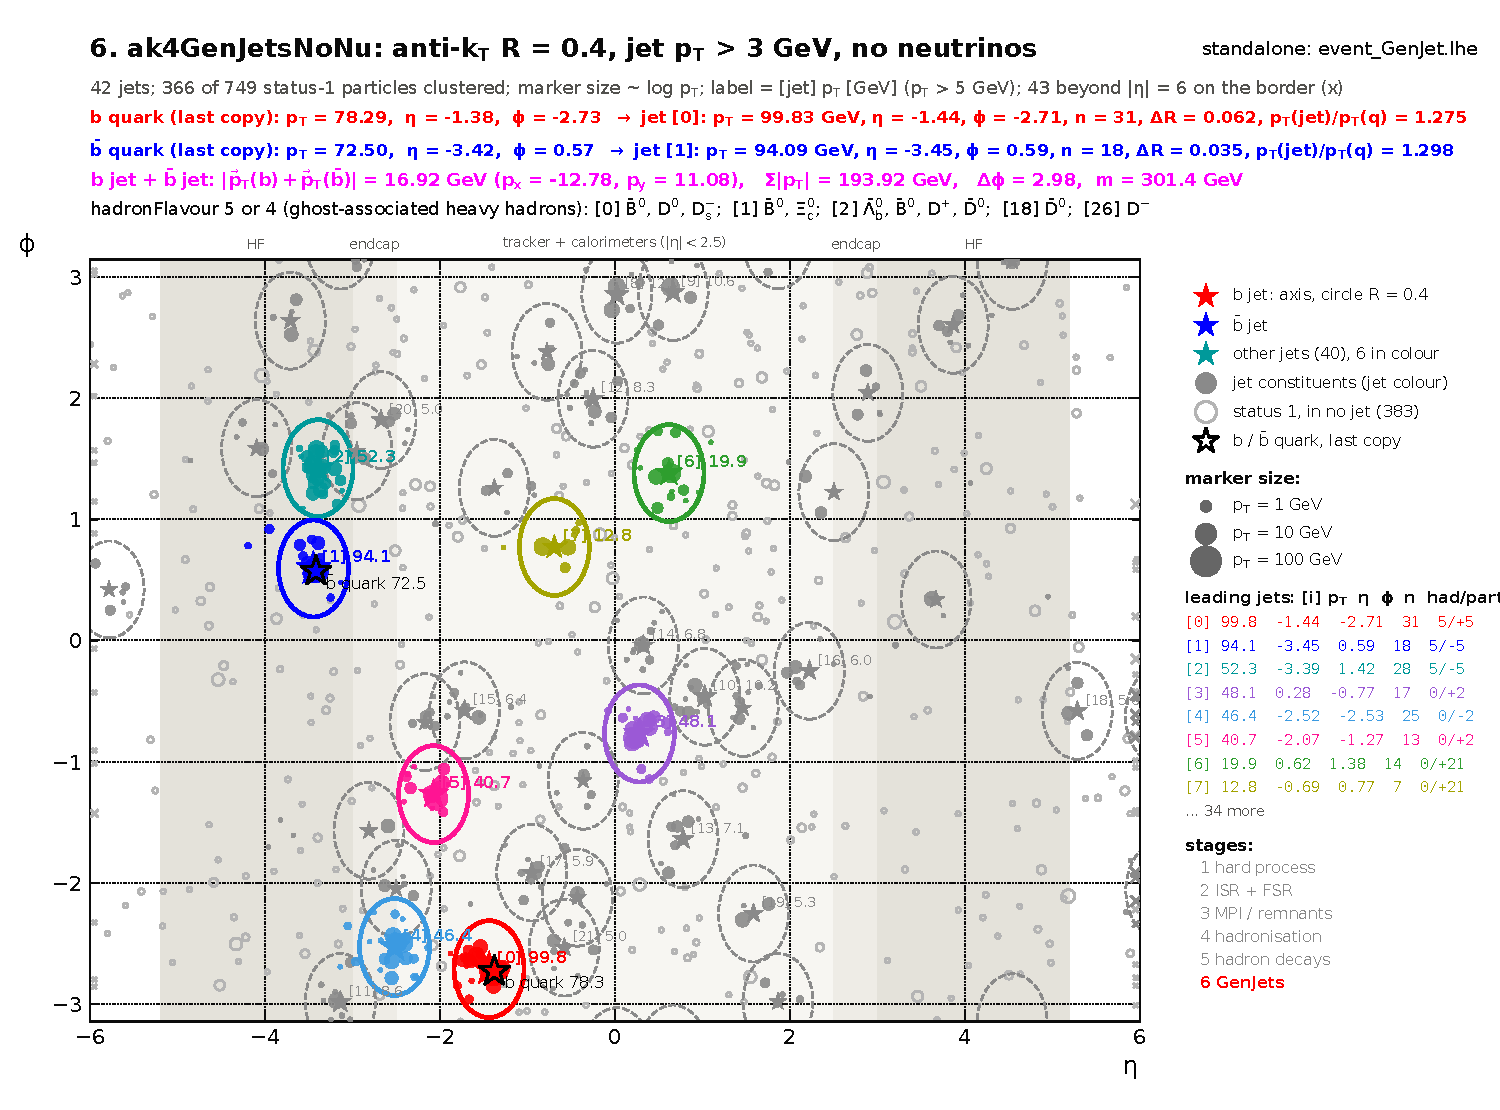
\includegraphics[width=0.84\textwidth]{GenJet/journey_GenJet_nonu.pdf}\\[1mm]
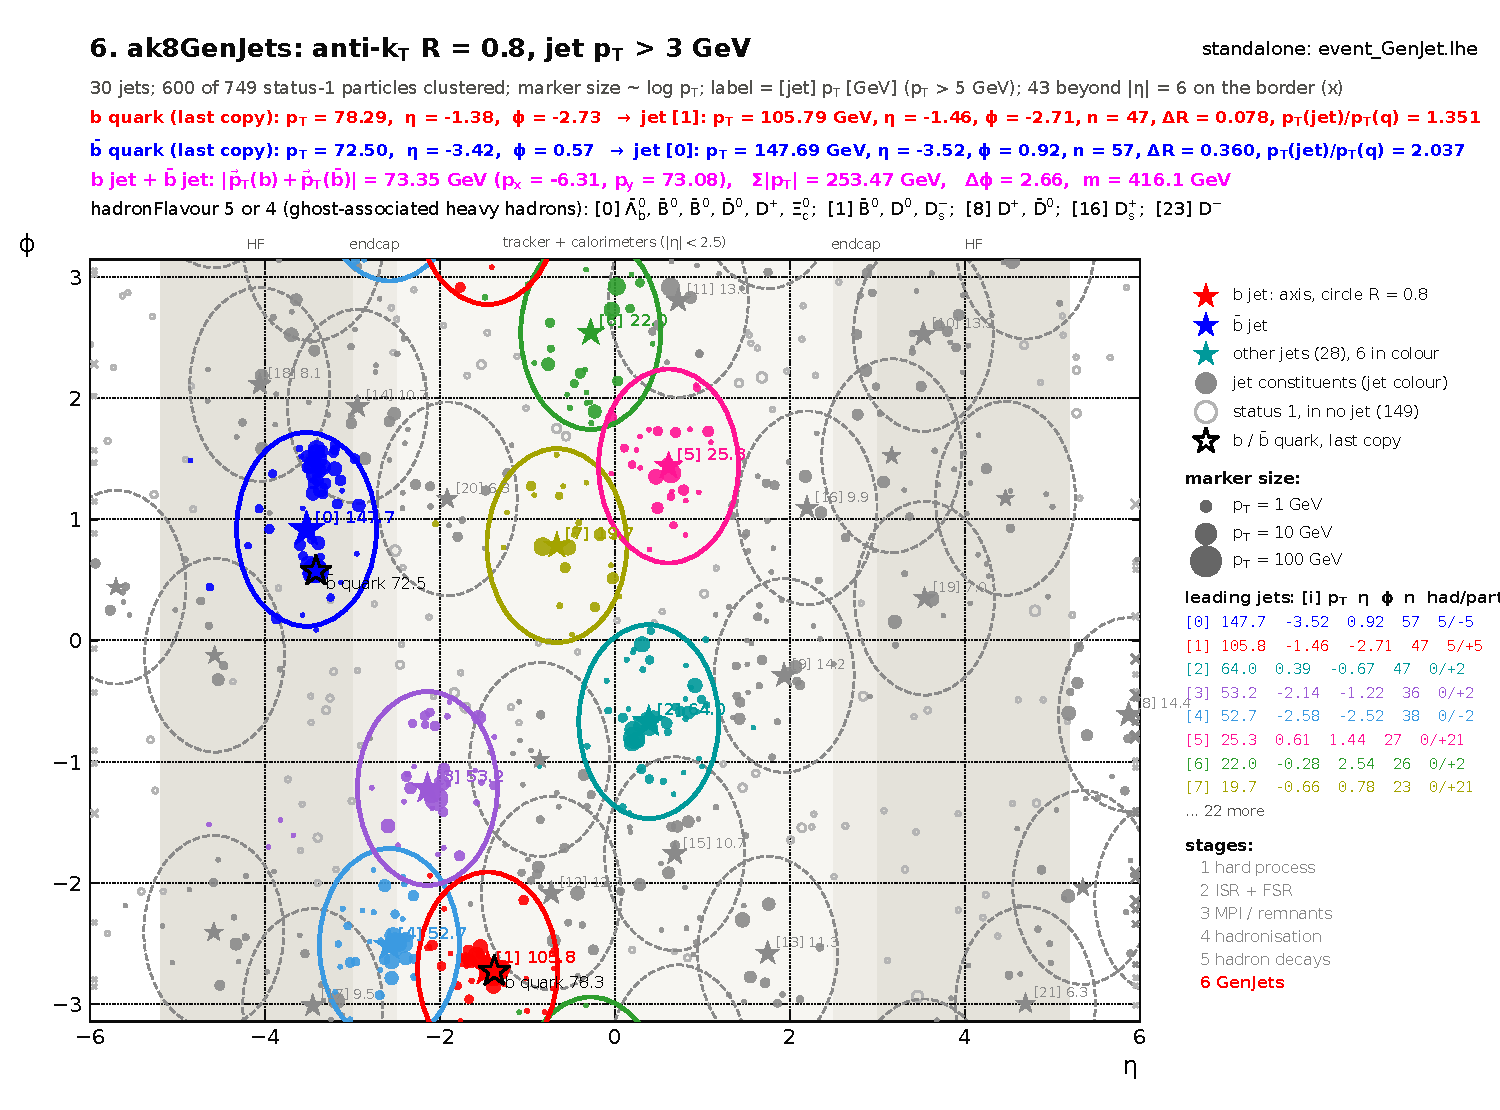
\includegraphics[width=0.84\textwidth]{GenJet/journey_GenJet_ak8.pdf}
\caption[The \akfournonu and \akeight jets of the event]{The other two
collections of our event, \akfournonu (top) and \akeight (bottom), in the
layout of \cref{fig:family_photograph:displays}. Without the neutrinos the
two $b$ jets are unchanged and the gluon pair's jet [2] loses its
$8.1\GeV$ neutrino; with $R=0.8$ the $\bar b$'s jet swallows the pair,
$147.69\GeV$ and three B~hadrons at $\dR=0.36$ from the quark, and the
$b$'s grows to $105.79$.}
\label{fig:family_photograph:journey_more}
\end{figure}

\paragraph{The same event in \CMSSW.} In \CMSSW this stop adds nothing to
the event and removes nothing from it: a step of its own, the process
\code{GENJET}, reads the complete generator event of
\cref{ch:children_producing_grandchildren}, runs \FASTJET's \antikt on its
$634$ stable particles and writes four collections, $R=0.4$ and $R=0.8$,
each with and without the neutrinos, above the $3\GeV$ of the standard
configuration. The \code{GEN} step had clustered jets already, as every
\code{GEN} step does, and those are dropped, so that the file holds one
set of jets, the one made here. What enters the clustering is decided by
a selector, not by the algorithm: every stable particle except a list of
hypothetical invisible ones, none of which occurs in this event, so that
all $634$ are offered to \akfour and, the three neutrino species added to
the list, $633$ to \akfournonu.

\akfour finds $27$ jets with $239$ of the $634$ particles in them. The
$b$ quark of status~71, the last copy before the hadronisation at
$\pt=91.74\GeV$ and $(\eta,\phi)=(-1.57,-2.08)$, is matched to jet [0]
of $117.79\GeV$ with $24$ constituents, $\dR=0.019$ from the quark, and
the constituents say where the momentum comes from: nine are the decay
products of the $B^-$ and carry $94.3\GeV$, seven more, $17.5\GeV$, are
hadrons from the mother's own string, the radiated energy coming back,
and the last eight, $6.4\GeV$, come from the strings of the multiparton
interactions and the remnants. The response of $1.284$ is the bookkeeping
of the shower, the reference quark having radiated already; against the
hard-process $b$ the same jet reads $1.04$. The $\bar b$ at $116.36\GeV$
and $\eta=-3.75$ is matched to jet [1] of $115.94\GeV$, $18$
constituents of which $16$ are the $B^{*+}$'s products, response $0.996$.
The pair of jets has a net \pt of $6.1\GeV$, the best balance of the
whole journey, where the two quarks had $25.1$.

Without the neutrinos the photograph loses a face. The $\bar b$'s jet is
unchanged and the mother's has become jet [1] of $79.82\GeV$ with $22$
constituents and a response of $0.870$: the $37.5\GeV$ of the electron
antineutrino of \cref{sec:children_producing_grandchildren:cmssw} are
gone, the axis moved with them and a pion of $0.5\GeV$ at the edge now
belongs to a neighbour, and the two leading jets have swapped places.
The pair is now $36.5\GeV$ out of balance, in her direction, which is
what a detector will call missing transverse momentum. In our own record
the two rows are equal, because our \Bbar decayed hadronically; the mean
of four hundred decays loses $7.7\GeV$, and the \CMSSW event is the tail
of that distribution once more. \akeight finds $28$ jets with $488$
particles in them, the mother's at $141.10\GeV$ with $55$ constituents
and a mass of $47\GeV$, $38$ of them with $28.5\GeV$ from strings other
than her own, and the $\bar b$'s at $121.01$ with $32$. The responses of
$1.28$ and $1.54$ are what ours are, $1.275$ and $1.351$: the status-71
quark is soft because the shower took its share, and the jet holds the
shower's gluons back plus the underlying event.

Panel~(b) of \cref{fig:family_photograph:displays} is the analyser's page
for \akfour: every jet above $3\GeV$ a circle of radius $R$ around its
axis, its constituents in the colour of the jet, the $395$ stable
particles in no jet grey, $38$ of them on the border, and the status-71
quarks as stars; the pages for \akfournonu and \akeight are in the
\code{JitJetSW} chapter that the companion links to. Set it next to
panel~(a) and to \cref{fig:family_photograph:journey_more}. The two are
different showers of the same hard event, so the comparison to make is
\cref{tab:family_photograph:numbers}; what the pictures share is the
structure, two hard circles on the two B~hadrons, four to six circles on
the gluon and quark jets of the shower, and a scatter of circles of a few
GeV on the underlying event, $27$ in one event and $42$ in the other,
with unclustered particles everywhere between them that no circle above
$3\GeV$ reached.

\begin{figure}[p]\centering
\ledgerdisplays
  {GenJet/journey_GenJet.pdf}
  {Standalone: the 42 \akfour jets of \file{example/GenJet/event_GenJet.lhe} (seed~1), drawn by \file{plot_journey_GenJet.py}.}
  {fig:family_photograph:journey}
  {GenJet/CMSSW/genJetAnalyzer_07_GenJet_AK4.pdf}
  {\CMSSW: the 27 \code{ak4GenJets} of the \code{07\_GenJet} job, drawn by the \code{genJetAnalyzer} of \code{JitJetSW}.}
  {fig:family_photograph:cmssw}
\caption[The \akfour jets of the event in the $(\eta,\phi)$ plane,
standalone and \CMSSW]{The \akfour jets of our event, standalone (a) and
\CMSSW (b). Every jet above $3\GeV$ is a circle of radius $0.4$, the $b$
jet red and the $\bar b$ jet blue with their constituents, the leading
other jets in colour; the particles in no jet are hollow in (a) and grey
in (b), and the last copies of the two quarks are stars. The headers give
the quark-to-jet matching with \dR and the response, the margins the
leading jets.}
\label{fig:family_photograph:displays}
\end{figure}

\subsection{What this stop is, and what it is not}
\label{sec:family_photograph:caveats}

The agreement in \cref{tab:family_photograph:numbers} with \FASTJET is
exact, and the parts of the chapter that are not a port of \FASTJET
carry their caveats:
\begin{itemize}
  \item \textbf{A photograph, not a truth.} The generator-level jet is
    a definition, and a different generator, tune or decay model gives a
    different one for the same hard event; the $21.5\GeV$ of gluons and
    underlying event in our jet are \PYTHIA's shower and CP5's
    multiparton interactions, and \cref{ch:paying_for_uninvited} will
    correct the reconstructed jet towards \emph{this} picture, not
    towards the quark.
  \item \textbf{The \akfournonu convention is CMS's.} ATLAS calibrates
    to jets that include the neutrinos from hadron decays and treats the
    difference in its $b$-jet uncertainties; a response quoted without
    saying which photograph it refers to is $8\%$ ambiguous for a $b$
    jet.
  \item \textbf{The ghost partons of \CMSSW are a selection.}
    \code{Pythia8PartonSelector} takes status 71 to 79, which the
    standalone record has as the rows the strings were built from; the
    ``physics'' partons of \CMSSW's \code{physicsPartons} collection are
    approximated here by the status-23 partons alone, and the
    \code{hadronFlavourHasPriority} switch that lets a $b$ hadron
    override a light \partflav is left off, as in the default
    configuration.
  \item \textbf{The sign of \partflav for a jet with both.} Jet [2] holds
    a $\bar b$ and a $b$ parton ghost and reads $-5$ from the harder; a
    jet from $g\to b\bar b$ carries one sign by that accident, as it does
    in \CMSSW.
  \item \textbf{IFN is a port of a paper, not of the code.} The
    trigger, the candidates and the recursion follow Section~3 of
    \cite{Caletti:2022glq}; the reference, the \FASTJET contrib, could
    not be run here, and a corner case might differ.
  \item \textbf{Flavour-$k_T$ without beam flavour.} The beams carry no
    flavour in the port; the paper's treatment of an initial-state
    heavy quark is not needed for a $b\bar b$ final state from light
    partons.
  \item \textbf{Hadron level with the heavy hadrons kept.} The safe
    definitions are run with the last $b$ and $c$ hadrons put back in
    place of their descendants, as the papers' hadron-level tests do;
    the neutrinos of their decays are then inside the hadron, and the
    jets of that run differ from \akfour at the border by a few hundred
    MeV.
  \item \textbf{The response is to the last copy.} $1.275$ divides by
    the quark of status 62 after the shower; the hard-process quark had
    $113.2\GeV$ and the response to it would be $0.88$. \CMSSW divides by
    the status-71 copy, the same object; the full chain's spread of $0.5$
    in that ratio is the denominator's, not the jet's.
  \item \textbf{One event is one sample.} The $42$ jets and the
    $0.40\GeV$ between jet and cone are this event's; the ensemble has
    $40.0\pm2.2$ and $0.84\pm0.59$, and the \CMSSW event $27$ jets.
\end{itemize}

\section{Further reading}
\label{sec:family_photograph:further_reading}
The \antikt algorithm is \cite{Cacciari:2008gp} and its implementation,
with the $N^2$ and $N\ln N$ strategies, the \FASTJET
manual~\cite{Cacciari:2011ma}; its ancestors are the $k_T$ algorithms of
\cite{Catani:1993hr,Ellis:1993tq} and the Cambridge/Aachen algorithm of
\cite{Dokshitzer:1997in,Wobisch:1998wt}, and the jet area that the same
ghosts measure is \cite{Cacciari:2008gn}. Infrared and collinear safety
begins with \cite{Sterman:1977wj} and is explained for jets in Salam's
``Towards jetography''~\cite{Salam:2009jx}. The infrared-safe flavour
definitions are flavour-$k_T$~\cite{Banfi:2006hf} with its application to
heavy-quark jets~\cite{Banfi:2007gu}, flavour anti-$k_T$~\cite{Czakon:2022khx},
flavour dressing~\cite{Gauld:2022lem} and interleaved flavour
neutralisation~\cite{Caletti:2022glq}, with the NNLO view of
\cite{Caletti:2022hnc} and the QCD-aware truth labelling of
\cite{Buckley:2015gua}; what they are needed for is the $Z+b$
calculation of \cite{Gauld:2020deh}. The experiment's side is the
$b$-tagging paper of CMS~\cite{CMS:2017wtu}, whose efficiencies are
measured against \hadflav, and the jet energy scale
paper~\cite{CMS:2016lmd}, whose reference is the jet without neutrinos;
the generators' side is \PYTHIA~8.3's guide~\cite{Bierlich:2022pfr} for
the status codes and \code{SlowJet}.

\begin{pitfalls}
\begin{itemize}[nosep]
  \item \textbf{Rapidity, not pseudorapidity.} \antikt measures \dR in
    $y$; the pictures are drawn in $\eta$. For a pion the two agree; a
    B~meson of $0.5\GeV$ placed at $y=0.1$ sits at $\eta=0.92$. The soft
    pair of the infrared test is placed in $y$, and a first version of
    the film drew it in $\eta$, outside both jets.
  \item \textbf{The cone is not the jet.} Same radius, same family,
    $99.43$ against $99.83\GeV$; the axis moved by $0.06$ and four soft
    particles changed sides. Compare a jet with a jet.
  \item \textbf{Three collections, three answers.} $99.83$, $99.83$ and
    $105.79\GeV$ in our event, and in the \CMSSW event $117.8$, $79.8$ and
    $141.1$. A response without the name of its collection is not a
    number.
  \item \textbf{The $3\GeV$ threshold is in the GEN file.} \akfour has
    $42$ jets here, and \code{slimmedGenJets} in a MiniAOD file keeps
    those above $8\GeV$; a matching to the nearest GenJet depends on
    which file one reads.
  \item \textbf{\hadflav has no sign and \partflav has one.} $5$ against
    $+5$ and $-5$; a $b$ jet from $g\to b\bar b$ reads $5$ from the
    hadrons and one sign from the harder parton.
  \item \textbf{The status-23 quark is not where the jet is.} $0.56$
    away in our event; the physics definition and the Run-1 $\dR<0.3$
    matching to status-3 partons find nothing. Use the ghosts.
  \item \textbf{A ghost must not merge into a jet of its own.} The beam
    distance of a ghost is $10^{36}/p_T^2$ under \antikt: it is swallowed
    long before it could be a jet. With $k_T$ ($p=+1$) it is
    $10^{-36}p_T^2$, the smallest number in the event: a ghost merges at
    once with whatever is nearest within $R$, sixteen times another ghost
    against three, and still ends in the nearest hard jet. The steps
    always number the pseudojets.
  \item \textbf{Net flavour reads the oscillation.} $+1$ for the
    $\bar b$ quark's jet; $17\%$ of the mother's decays read $-1$. The
    net flavour of a jet is the hadron's at decay, not the quark's.
  \item \textbf{The gluon's pair is one jet at $R=0.4$ and part of the
    $\bar b$'s at $0.8$.} Jet [2] with \hadflav $5$ and net $0$ is a
    $g\to b\bar b$ jet, the kind a tagger calibrated on single-$b$ jets
    misjudges; at $R=0.8$ it disappears into the $\bar b$'s jet, which
    then reads three B~hadrons.
  \item \textbf{Infrared safety is about labels too.} A jet's \pt is
    safe under a soft massless pair, its \hadflav is not; our pair is soft
    in \pt only and moves jets [8] and [9] by $0.2$ and $1.0\GeV$. Run
    the scan of \cref{fig:family_photograph:irsafety_plot} on any new
    definition.
  \item \textbf{IFN with $\alpha=2$ ignores the soft one's \pt.}
    $\max(p_T)^2\Omega^2$ for both the merge and the candidate; what
    decides is which hard object the soft flavour is closer to in
    $\Omega^2$, scaled by that object's $p_T^2$.
  \item \textbf{Response to which quark?} $1.275$ to the last copy,
    $0.88$ to the hard-process quark; the full chain's response has a
    width of $0.5$ because its denominator moves.
  \item \textbf{Three decimals.} The record carries three decimals and
    the scripts recompute $E$ from the mass; a $\pi^-$ of $0.27\GeV$ on
    the $R=0.8$ border makes its \akeight jet, $105.79\GeV$ in $47$
    particles, differ from entry~0 of the full-precision ensemble,
    $105.51$ in $46$.
\end{itemize}
\end{pitfalls}

\begin{exercises}
\item \textbf{Run it.} Run \file{standalone_genjets.py} and confirm $42$
  \akfour jets, $99.83\GeV$ and $31$ constituents for jet [0],
  $\hadflav=5$ and $\partflav=+5$. Run \code{--algorithm kt} and
  \code{ca} and count the jets above $3$, $10$ and $30\GeV$; which
  algorithm makes the most jets above $3\GeV$ and why?
\item \textbf{The distance.} From the log's first merge, $K^-$ of
  $10.567\GeV$ and $\pi^-$ of $4.451$ at $\dR=0.006$, reproduce
  $\dij=1.74\times10^{-6}$ with \cref{eq:family_photograph:dij}; then
  compute \diB for the finished jet and check that it exceeds the last
  merge's \dij. What would the first merge have been with $p=+1$?
\item \textbf{The profile.} With \code{--radius} from $0.1$ to $1.2$
  reproduce panel~(a) of \cref{fig:family_photograph:truejet_plot} for
  the jet, and from the record the cone; at which $R$ does the gluon jet
  [4] enter, and what is its \pt?
\item \textbf{The threshold.} Count the \akfour jets above $5$, $8$,
  $15$ and $20\GeV$ from the jet table; how many of the $42$ have a
  single constituent, and what are they?
\item \textbf{The neutrino.} Run the decay script of
  \cref{ch:children_producing_grandchildren} with \code{--seed 4}, then
  this script on its output, and reproduce $99.6$ and $90.2\GeV$ for the
  two \akfour collections. From \file{standalone_genjet_stats.stats.json}
  reproduce $91.93\pm12.12$, the $54\%$ without a neutrino and the $37\%$
  above $5\GeV$.
\item \textbf{The ghost.} Compute $d_{\mathrm{ghost},j}$ and
  $d_{\mathrm{ghost},B}$ of \cref{eq:family_photograph:ghost} for the
  \Bbar's ghost against the pseudojet of $22.16\GeV$ it joined at
  $\dR=0.031$; then change \code{GHOST\_RESCALING} to $10^{-6}$ and find
  the first jet whose \pt changes in the sixth digit.
\item \textbf{The labels.} From the jet table reproduce the labels of
  jets [0], [1] and [2] from the ghosts listed with each; then explain
  from the record why jet [1] reads net $+1\,b$ and jet [2] reads $0$.
\item \textbf{The physics definition.} From rows 6 and 719 of the record
  compute the \dR between the status-23 $b$ quark and its last copy, and
  from \file{event_PS.lhe} find the branching that moved it most. For
  which $R$ does the status-23 ghost enter the $b$ jet?
\item \textbf{The whisper.} Run \code{--soft-pair} at $0.2$, $0.5$, $1$,
  $2$ and $5\GeV$ and tabulate the four labels of jets [8] and [9];
  reproduce $\uik=0.064$ and $u_{ij}=0.21$ at $0.5\GeV$ from
  \cref{eq:family_photograph:ifn} and the log's positions. At what \pt
  does IFN stop neutralising, and why there?
\item \textbf{$\Omega^2$.} Plot $\Omega^2$ of \cref{eq:family_photograph:ifn}
  against $\dR^2$ for $\Delta\phi=0$ and $\Delta y$ from $0$ to $3$, and
  find the $\Delta y$ at which the two differ by a factor two; what does
  that do to a $\bar b$ hadron at $\eta=-3.4$ as a candidate for the
  mother's $b$ at $-1.4$?
\item \textbf{Flavour-$k_T$.} From \cref{eq:family_photograph:fkt} and the log
  of \code{--soft-pair 0.5} explain why the two flavoured pseudojets,
  $0.58$ apart, merge instead of becoming two jets; then
  compare the flavour-$k_T$ jet of the mother, $17$ constituents, with
  the \antikt one, $31$: which particles differ?
\item \textbf{The ensemble.} From the statistics file compute the mean
  and the width of the jet minus the cone at $R=0.4$ and at $0.8$,
  reproduce $0.84\pm0.59$ and $-2.60\pm0.62$, and explain the sign at
  $0.8$.
\item \textbf{\FASTJET by hand.} Run the validation script, then change
  the recombination scheme in it to \code{pt\_scheme} and find how far
  the jet masses move; then run \code{SlowJet} with \code{massSet = 0}
  and explain the change in the rapidities.
\item \textbf{The \CMSSW pages.} From the header of panel~(b) of
  \cref{fig:family_photograph:displays} and from the log of the jet
  analyser (the companion says where the files are)
  reproduce the responses $1.284$, $0.870$ and $1.538$ and the $37.5\GeV$
  of neutrino from the difference of the first two; then explain why the
  $\bar b$'s jet has the same \pt with and without the neutrinos.
\item \textbf{Film it.} Run the animation with \code{--scene whisper}
  and, from the \code{-v} log of \code{--soft-pair 0.5}, predict before
  watching the two distances that the neutralisation line will quote.
\end{exercises}

\subsection*{Open problems in the context of Phase-2 LHC}
\label{sec:family_photograph:open_problems}

The photograph is a convention, and the High-Luminosity LHC will stretch
every convention in it: jets at two hundred collisions per crossing need
a reference whose own ambiguities are smaller than the corrections of
\crefrange{ch:paying_for_uninvited}{ch:the_receipt}, and measurements of
$t\bar t+b\bar b$, $Z+b$ and $H\to b\bar b$ at the precision of
\cite{Azzi:2019yne} need a flavour definition that a calculation can
share with the experiment. Each of the following can be started with
the scripts of this chapter.
\begin{enumerate}
  \item \textbf{A safe flavour label in the experiments.} \hadflav is
    what CMS and ATLAS calibrate their taggers against, and it is not
    infrared safe; IFN~\cite{Caletti:2022glq}, flavour
    anti-$k_T$~\cite{Czakon:2022khx} and flavour dressing~\cite{Gauld:2022lem}
    are, and keep the \antikt jets, so that for the first time the
    experiments could label their simulated jets with the definition a
    NNLO calculation~\cite{Gauld:2020deh,Caletti:2022hnc} uses. The open
    question is practical: how often do the labels differ in a $b$-jet
    sample, and in which jets? With the ensemble's \code{net} and
    \code{ifn} entries and the \code{--soft-pair} scan, measure the
    fraction of jets whose \hadflav and IFN labels disagree as a function
    of the jet \pt and of the $g\to b\bar b$ rate, which
    \cref{ch:mother_gives_birth} can vary; the Phase-2 question is
    whether a tagger calibrated against a safe label loses efficiency on
    the gluon-splitting jets it no longer counts as $b$.
  \item \textbf{The neutrino in the reference.} CMS corrects to the jet
    without neutrinos and ATLAS to the jet with them, and the
    difference, $8\GeV$ on average and $12$ in width for the mother's
    jet, is absorbed in $b$-jet energy scale uncertainties and in the
    regressions of \cite{CMS:2019uxx}. At the HL-LHC the top-quark mass
    and the $H\to b\bar b$ signal strength will be limited by exactly
    this term~\cite{Azzi:2019yne}. From the ensemble, measure how much of
    the $12\GeV$ a photograph that keeps the neutrino's direction but
    not its energy, or one that adds the soft lepton's momentum back,
    would recover; the question is which reference definition minimises
    the data-to-simulation uncertainty of a $b$ jet rather than its
    resolution.
  \item \textbf{The radius at two hundred pileup.} The profile of
    \cref{eq:family_photograph:ptR} rises by $9\GeV$ from $R=0.4$ to
    $0.8$ for our family and the underlying event adds a GeV per tenth
    of a unit; at the HL-LHC the pileup of \cref{ch:crowd_on_the_road}
    adds $0.9\GeV$ per unit of area per collision at the generator level,
    $0.6$ after the detector, before subtraction.
    With the profile of the ensemble and the pileup density of
    \cref{ch:paying_for_uninvited}, find the radius at which the
    family's own radiation lost outside equals the pileup fluctuation
    inside, as a function of the jet \pt; the question, raised for Run~2
    in \cite{CMS:2016lmd} and open for Phase~2, is whether $0.4$ is still
    the right photograph for a $100\GeV$ $b$ jet at $\langle\mu\rangle=200$.
  \item \textbf{Truth for substructure.} The $\bar b$'s \akeight jet
    holds three B~hadrons and two families; the boosted top of
    \cref{ch:three_families} will hold three partons' families in one
    circle, and its truth definition, which partons and which hadrons
    belong, is as much a convention as this chapter's. With the
    constituent table and the ghosts of the \akeight jets, define the
    ``truth'' of a two-family jet three ways, by the ghosts, by the
    status-23 partons and by IFN, and measure how often they agree; the
    question is which definition the substructure taggers of
    \cref{ch:three_families} should be calibrated against at the HL-LHC.
  \item \textbf{Generator dependence of the photograph.} The $21.5\GeV$
    of gluons and underlying event in the reference jet are \PYTHIA's
    and CP5's, and a different shower or tune moves the reference by a
    GeV without touching the quark; the jet energy corrections of
    \cref{ch:paying_for_uninvited} inherit that GeV as a flavour and
    generator uncertainty~\cite{CMS:2016lmd}. With the \code{full} mode of
    the validation script under different tunes and showers, measure the
    spread of the mother's \akfournonu response; the Phase-2 question,
    raised for all generators in \cite{HSFPhysicsEventGeneratorWG:2020gxw},
    is whether the reference of the corrections can be defined at the
    hadron level with an uncertainty below the half percent the HL-LHC
    jet energy scale aims for.
\end{enumerate}
The next stop puts the family on the road, where it meets the other
collisions of the same bunch crossing, and the photograph taken here is
what will tell the family from the crowd.

\part{On the Road: Crowds, Borders and Checkpoints}
%% ---------------------------------------------------------------------------
% Chapter 8: The Crowd on the Road: Pileup
% The scripts, records, logs and films of this stop live in example/PU/, and
% the technical companion of the chapter is chapter/chapter_08_PU.md: how to
% run the scripts, how to read the records and logs, how the official numbers
% were obtained, and the full tables. The book gives the physics.
% The crowd is the crowd of Run 3 (2024): sixty collisions per crossing at
% 13.6 TeV, the 2024 beam spot, the production window bx = -12 ... +3.
% ---------------------------------------------------------------------------
%% chapter-local shorthands
\providecommand{\akfour}{\code{ak4GenJets}\xspace}
\providecommand{\akfournonu}{\code{ak4GenJetsNoNu}\xspace}
\providecommand{\mup}{\ensuremath{\mu}\xspace}
\providecommand{\mutrue}{\ensuremath{\mu_{\mathrm{true}}}\xspace}
\providecommand{\rhoPU}{\ensuremath{\rho}\xspace}
\providecommand{\sigmainel}{\ensuremath{\sigma_{\mathrm{inel}}}\xspace}
\providecommand{\bx}{\ensuremath{\mathrm{bx}}\xspace}
\providecommand{\ns}{\ensuremath{\,\mathrm{ns}}\xspace}
\providecommand{\ps}{\ensuremath{\,\mathrm{ps}}\xspace}
\providecommand{\cm}{\ensuremath{\,\mathrm{cm}}\xspace}
\providecommand{\um}{\ensuremath{\,\mu\mathrm{m}}\xspace}
\providecommand{\mbarn}{\ensuremath{\,\mathrm{mb}}\xspace}
\providecommand{\Mix}{\code{MixingModule}\xspace}
% written by minbias_catalogue.py: three tables of the minimum-bias library (do not edit)
\newcommand{\minbiasCatalogueTen}{%
\begin{tabular}{rlrrrrrrrrrrr}\toprule
event & proc. & interactions & stable & charged & central & $|\eta|>5.5$ & lead \pt & $\Sigma\pt$ & jets $>10$ & fwd $p$ & $z$ [cm] & $t$ [ns] \\ \midrule
1142 & ND & 1 & 74 & 32 & 2 & 27 & 0.88 & 21.0 & 0 & 1 & $-0.96$ & $-0.227$ \\
1143 & ND & 22 & 515 & 232 & 100 & 43 & 3.77 & 252.1 & 0 & 0 & $+1.10$ & $-0.006$ \\
1144 & ND & 23 & 511 & 240 & 62 & 86 & 4.17 & 225.4 & 1 & 0 & $-4.84$ & $+0.035$ \\
1145 & ND & 1 & 76 & 38 & 2 & 31 & 1.71 & 25.3 & 0 & 0 & $+0.90$ & $+0.150$ \\
1146 & ND & 28 & 560 & 264 & 102 & 63 & 4.11 & 288.5 & 0 & 0 & $+1.08$ & $+0.166$ \\
1147 & ND & 17 & 438 & 194 & 57 & 68 & 3.98 & 195.4 & 0 & 0 & $-1.60$ & $+0.096$ \\
1148 & SD & 1 & 32 & 12 & 0 & 19 & 1.85 & 11.3 & 0 & 1 & $-1.15$ & $-0.083$ \\
1149 & ND & 11 & 463 & 186 & 62 & 61 & 4.80 & 213.0 & 1 & 0 & $+0.97$ & $-0.044$ \\
1150 & ND & 19 & 345 & 148 & 37 & 59 & 4.49 & 154.7 & 0 & 0 & $-2.60$ & $+0.145$ \\
1151 & ND & 2 & 82 & 40 & 5 & 18 & 1.44 & 29.7 & 0 & 0 & $-2.61$ & $-0.073$ \\
\bottomrule\end{tabular}}
\newcommand{\minbiasCatalogueSummary}{%
\begin{tabular}{lrrrr}\toprule
per collision & mean & median & min & max \\ \midrule
interactions & 6.0 & 2 & 1 & 45 \\
stable particles & 179 & 116 & 3 & 829 \\
charged stable particles & 83 & 54 & 2 & 374 \\
central ($|\eta|<2.5$, $\pt>0.5\GeV$) & 19 & 8 & 0 & 167 \\
beyond $|\eta|=5.5$ & 37 & 34 & 2 & 108 \\
\pt of the hardest particle [GeV] & 2.17 & 1.7 & 0.1 & 17.9 \\
scalar sum of \pt [GeV] & 73 & 38 & 1 & 518 \\
\antikt $R=0.4$ jets above $10\GeV$ & 0.15 & 0 & 0 & 7 \\
forward protons ($\xi<0.55$) & 0.38 & 0 & 0 & 2 \\
vertex $z$ [cm], the 960 drawn & $0.22$ & $0.30$ & $-12.4$ & $13.9$ \\
vertex $t$ [ns], the 960 drawn & $0.003$ & $-0.001$ & $-0.35$ & $0.38$ \\
\bottomrule\end{tabular}}
\newcommand{\minbiasCataloguePerProcess}{%
\begin{tabular}{lrrrrrrrr}\toprule
per process & events & $\sigma$ [mb] & interactions & stable & charged & central & lead \pt [GeV] & $\Sigma\pt$ [GeV] \\ \midrule
non-diffractive (ND) & 1425 & 55.42 & 8.1 & 230 & 106 & 25 & 2.6 & 95 \\
single diffractive (SD) & 319 & 12.86 & 1.0 & 51 & 24 & 4 & 1.2 & 17 \\
double diffractive (DD) & 219 & 8.85 & 1.0 & 62 & 29 & 4 & 1.2 & 21 \\
central diffractive (CD) & 37 & 1.29 & 1.0 & 28 & 14 & 2 & 0.9 & 9 \\
\bottomrule\end{tabular}}

\chapter{The Crowd on the Road: Pileup}
\chaptermark{The Crowd on the Road}
\label{ch:crowd_on_the_road}

\begin{journeybox}
Our family is not alone. At every bunch crossing some sixty other families
set out at the same moment, and the road is so crowded that some of their
members walk in step with ours and are impossible to tell apart. The road
is the road of Run~3 in its last full year, 2024: the crowd of this
chapter is the one CMS recorded, and the one its simulation was built to
reproduce, and the family will meet it again at every stop ahead.
\end{journeybox}

\physicsline{the mean number of collisions per bunch crossing,
$\mup=L\sigmainel/(n_b f_{\mathrm{rev}})$, and its Poisson fluctuation; the
minimum-bias collision and its four kinds; in-time and out-of-time pileup,
the 25\ns clock and the sixteen crossings of the production window; the
beam spot of 2024, where and when the collisions happen; how \CMSSW mixes
a library of soft collisions into a signal event, why the production
premixes, and how a flat pileup profile is reweighted; the median energy
density \rhoPU, the jet area $A$ and the subtraction $\pt-\rhoPU A$. The
one number to take away: at $\mup=60$ the crowd puts $59\GeV$ into every
unit of area of the $(\eta,\phi)$ plane, thirty GeV of strangers into our
hundred-GeV jet, and the subtraction removes them on average, not event by
event: $\pm7\GeV$ stay.}

\section{What we will see at this stop}
\label{sec:crowd_on_the_road:what_we_compute}

At the end of \cref{ch:family_photograph} the photograph was taken: jet [0]
of \akfour, $99.83\GeV$ in $31$ particles around $\eta=-1.44$, $\phi=-2.71$,
the reference every later jet will be judged against. The family was alone
in the picture. It never is in the detector. The LHC does not collide one
proton with one proton; it collides bunches of $10^{11}$ protons every
$25\ns$, and at the luminosity the LHC delivered in 2024, about sixty pairs
of protons collided inelastically in each crossing. One of those collisions
is ours, the $q\bar q\to b\bar b$ of \cref{ch:ancestral_home}. The other
sixty happened because they could, soft and uneven, and their particles
land in the same detector at the same moment, on top of our family, inside
the circle of our jet. They are called pileup, and they are the crowd on
the road. This stop is about the crowd itself: how large it is and why,
what one member of it carries, where and when along the beam line it
walks, and how much of it falls inside our jet before any detector has
seen a single particle. The mitigation, the tracks that point back to the
right vertex, is the business of
\crefrange{ch:crossing_the_border}{ch:the_police}; the correction that
pays for what cannot be removed is \cref{ch:paying_for_uninvited}. Here we
only let the crowd arrive and measure what it does.

The crowd is the crowd of 2024, and the choice deserves a sentence. The
family of \crefrange{ch:ancestral_home}{ch:family_photograph} was born at
$\sqrt{s}=13.6\TeV$, the energy of Run~3, and Run~3 is over: its
luminosity, its filling scheme, its beam spot and its detector are
frozen, measured, and written into the conditions of \CMSSW, so that a
book pinned to them stays right. The High-Luminosity LHC, with its two
hundred collisions per crossing and the detector CMS is building for
them, is still being designed, and a book pinned to it would be out of
date before the first beam. So the crowd of every stop from here on is
the Run-3 crowd, the detector of \cref{ch:crossing_the_border} is the
2024 CMS detector, and what the HL-LHC will change is said at the end of
each chapter, in its open problems, where the scripts of this stop keep
the HL-LHC road one option away.\footnote{\file{standalone_pileup.py
--scenario ultimate} mixes the same family at $\mup=200$ with the Phase-2
luminous region, and the exercises and open problems use it.}

The numbers to take away are four. The crowd of our crossing has $63$
collisions, a Poisson draw with mean $60$, and brings $12\,113$ particles
to the $744$ of the family, $860$ charged ones into the tracker's reach
against $93$. It puts $68\GeV$ into every unit of area of the
$(\eta,\phi)$ plane in this crossing, $59$ on average, $0.94$ per
collision, so that the circle of our jet, $0.53$ units of area, receives
$33.61\GeV$ of strangers from $34$ different collisions and reads
$132.75\GeV$ instead of $99.83$. The subtraction $\pt-\rhoPU A$ takes
$36.09\GeV$ back out and leaves $96.66$, three GeV below the truth in this
crossing and $-2\pm7\GeV$ from it over four hundred draws of the crowd:
the average is removed, the fluctuation is not, and that fluctuation is
the first term of the resolution of a jet in Run~3. And the collisions are
spread over $\pm3.6\cm$ along the beam and $\pm120\ps$ in time, the
nearest one to ours a twentieth of a millimetre away in this crossing and
a millimetre on the median, which is the room the vertex finder will have
to work in, with no timing layer to help it. As at the previous stops we
meet the numbers four times, from the top down: a film shows the
photograph of \cref{ch:family_photograph} disappearing under the crowd
collision by collision, the beam spot and the 25\ns clock, one member of
the crowd, the median that measures it, our jet filling up and being
subtracted, and the crowd drawn four hundred times; a Python file, needing
only NumPy, mixes a library of two thousand minimum-bias collisions into
the record in the way \CMSSW's \Mix does, clusters the result with the
\antikt of \cref{ch:family_photograph} and ghosts, and writes \rhoPU, the
areas and the subtracted jets; the theory derives \mup from the
luminosity, the collision from the cross section, the beam spot from two
bunches and \rhoPU from the median; and the official packages, \PYTHIA for
the library and its cross sections, \FASTJET for the areas and the two
estimators of \rhoPU on exactly our mixed particles, and the 2024 \CMSSW
mixing of the companion, get the last word.

\paragraph{The film.}
\label{sec:crowd_on_the_road:animation}
The film first: the eighth on the playlist of \jitjetworld puts the
photograph into the crowd in six narrated scenes, every number on the
screen read from the record and the ensemble that the script wrote. The
voice picks up where the film of \cref{ch:family_photograph} stopped, the
photograph is taken, and ends at the next stop, the border of the
detector. The $651$ signal particles sit in the $(\eta,\phi)$ plane with
their jet circles, and the $63$ collisions of the crossing stack onto
them one by one, a counter running and \rhoPU rising by a GeV per
collision until the plane is khaki and \antikt finds $173$ jets; the beam
spot appears as the overlap of two bunches, the vertices of our crossing
spread along it with the signal among them, and the fifteen neighbouring
crossings of the production window arrive $25\ns$ apart; the four kinds
of minimum-bias collision are drawn one after the other, each with its
row in the table of cross sections and multiplicities, and the
multiplicity of all two thousand builds up; the grid cells fill
with transverse momentum and their median settles at \rhoPU; the family's
circle fills with strangers, the counter climbs from $99.8$ to
$132.7\GeV$, and $\rhoPU A$ is taken out; and the crowd is drawn four
hundred times on the same photograph, the pileup inside the circle and
the residual after the subtraction filling their histograms.
\Cref{fig:crowd_on_the_road:stills} shows one key frame per scene. Watch
first, and let the formulae catch up.

\begin{figure}[htbp]\centering
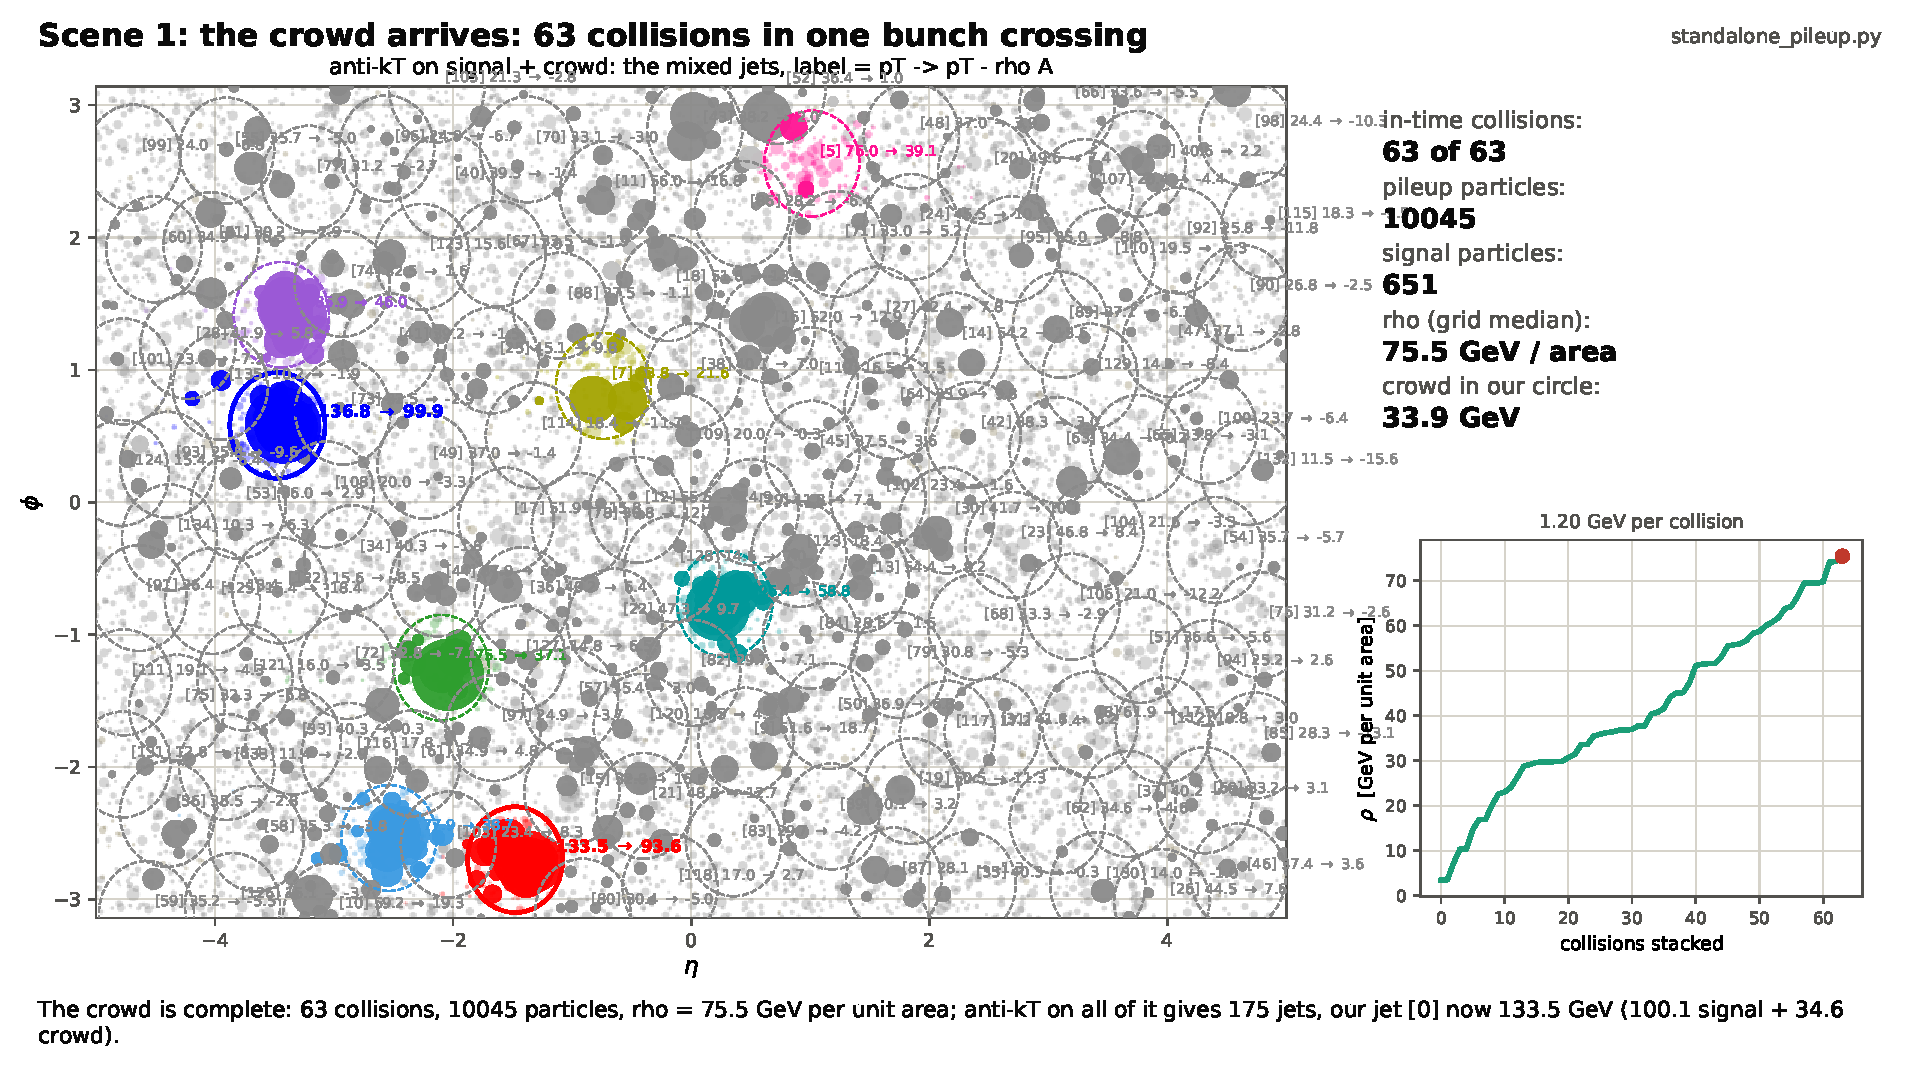
\includegraphics[page=1,width=0.325\textwidth]{PU/Standalone/animate_standalone_pileup_stills.pdf}\hfill
\includegraphics[page=2,width=0.325\textwidth]{PU/Standalone/animate_standalone_pileup_stills.pdf}\hfill
\includegraphics[page=3,width=0.325\textwidth]{PU/Standalone/animate_standalone_pileup_stills.pdf}\\[1.5mm]
\includegraphics[page=4,width=0.325\textwidth]{PU/Standalone/animate_standalone_pileup_stills.pdf}\hfill
\includegraphics[page=5,width=0.325\textwidth]{PU/Standalone/animate_standalone_pileup_stills.pdf}\hfill
\includegraphics[page=6,width=0.325\textwidth]{PU/Standalone/animate_standalone_pileup_stills.pdf}
\caption[Key frames of the animated standalone pileup stage]{Key frames of
the six scenes of the animated standalone pileup stage, drawn by
\file{animate_standalone_pileup.py} with \code{--stills}, in reading
order. The crowd arriving on the photograph; the beam spot and the
sixteen crossings on the clock; the four kinds of collision and the library;
the grid cells and their median; our jet filling up and being
subtracted; the crowd drawn four hundred times. The film itself is the
eighth on the playlist of \jitjetworld.}
\label{fig:crowd_on_the_road:stills}
\end{figure}

\paragraph{The picture to carry: the crowd.}
The two halves of \cref{fig:crowd_on_the_road:crowd_sketch} are the whole
chapter. On the left, one bunch crossing: two bunches of protons pass
through each other, and wherever and whenever they overlap a collision
can happen, sixty of them in a region $4\cm$ long and an eighth of a
nanosecond wide, one of them ours. Nothing selects it; the detector
records the crossing because our collision fired the trigger, and the
other sixty come free, as do the crowds of the twelve crossings before
and the three after, which the slow detectors remember. On the right, the
circle of our jet in the $(\eta,\phi)$ plane: the family, thirty-one
particles within a tenth of a unit of the axis, and the strangers,
sixty-five soft particles from thirty-four collisions scattered evenly
over the circle, a third as many GeV as the family itself. Two things in
the picture matter for everything that follows. The crowd is
\emph{uniform on average and uneven in every event}: its mean density
\rhoPU is one number for the whole plane and can be measured from the
empty parts of the plane and subtracted from the full ones, and that
subtraction is exact only for the mean, because the number of collisions,
the number of particles each brings and where they land all fluctuate,
and what they leave behind in a circle of area $0.5$ is $\pm7\GeV$ wide.
And the crowd is \emph{soft}: its hardest particle is $2\GeV$ on average,
its members make jets of their own above $30\GeV$ only before \rhoPU is
subtracted and never after, and what they do to our jet is a pedestal,
not a disguise; a fake jet of the crowd is rare, a true jet with the
crowd on top is every jet. The rules are the jet-area paper of Cacciari
and Salam~\cite{Cacciari:2007fd} and the catchment area of
jets~\cite{Cacciari:2008gn}, the \FASTJET manual~\cite{Cacciari:2011ma},
the \CMSSW \Mix and its \code{BetafuncEvtVtxGenerator}; the experiment's
view of the crowd is the pileup mitigation paper of
CMS~\cite{CMS:2020ebo}, and the theorist's the review of
Soyez~\cite{Soyez:2018opl}.

\begin{figure}[htbp]\centering
\resizebox{\textwidth}{!}{% ---------------------------------------------------------------------------
% The picture to carry: (a) one bunch crossing of Run 3 (2025), sixty
% collisions along the beam spot, ours among them; (b) the circle of our jet
% in the (eta, phi) plane: the family and the strangers that walked in, with
% the numbers of the 400-draw ensemble of standalone_pileup.py --repeat.
% ---------------------------------------------------------------------------
\begin{tikzpicture}[x=1cm,y=1cm,
  every node/.style={font=\footnotesize},
  lab/.style={font=\scriptsize,align=center},
  head/.style={font=\small\bfseries},
  fam/.style={circle,fill=red!80!black,inner sep=0pt,minimum size=4pt},
  crowd/.style={circle,fill=olive!60!brown,inner sep=0pt,minimum size=2.6pt},
  vtx/.style={circle,fill=cyan!60!blue,inner sep=0pt,minimum size=2.6pt},
  ring/.style={red!80!black,line width=1.2pt}]
% ---------------- (a) the bunch crossing ----------------------------------------------------------
\begin{scope}
\node[head,anchor=west] at (-0.3,3.2) {(a) one bunch crossing of 2025: $\mu=60$ collisions along $z$};
% the two bunches moving towards each other
\fill[blue!25] (-4.2,0.9) ellipse (1.6 and 0.32);
\fill[orange!35] (4.2,0.9) ellipse (1.6 and 0.32);
\draw[-{Stealth[length=2mm]},blue!60!black,thick] (-2.4,1.35) -- (-1.4,1.35) node[lab,above,pos=0.5] {beam 1};
\draw[-{Stealth[length=2mm]},orange!80!black,thick] (2.4,1.35) -- (1.4,1.35) node[lab,above,pos=0.5] {beam 2};
\node[lab,text=blue!60!black] at (-4.2,0.45) {$10^{11}$ protons per bunch};
\node[lab,text=orange!80!black] at (4.2,0.45) {every 25 ns};
% the beam spot: a Gaussian along z, sigma_z = 3.6 cm (scale: 0.25 cm per cm)
\draw[-{Stealth}] (-4.5,-0.3) -- (4.5,-0.3) node[below left,lab] {$z$ [cm]};
\foreach \x/\t in {-4/$-16$,-2/$-8$,0/0,2/8,4/16} {\draw (\x,-0.35) -- (\x,-0.25); \node[lab,anchor=north] at (\x,-0.4) {\t};}
\draw[green!50!black,thick] plot[domain=-4.5:4.5,samples=80] (\x,{-0.3+1.1*exp(-(\x-0.1)*(\x-0.1)/(2*0.9*0.9))});
\node[lab,text=green!50!black,anchor=west] at (1.2,0.75) {$\sigma_z=3.6$ cm, $\sigma_t=120$ ps};
% 60 vertices drawn along z (pseudo-random, Gaussian-like by summing uniforms)
\pgfmathsetseed{8}
\foreach \i in {1,...,60} {
  \pgfmathsetmacro{\zz}{0.1+0.9*(rand+rand+rand)*0.58}
  \pgfmathsetmacro{\yy}{-0.3+0.08+0.5*rnd*exp(-\zz*\zz/(2*0.9*0.9))}
  \node[vtx] at (\zz,\yy) {};
}
\node[star,star points=5,fill=red!80!black,inner sep=0pt,minimum size=9pt] at (-0.05,0.05) {};
\node[lab,text=red!80!black,anchor=north] at (-0.05,-0.05) {ours};
\node[lab,anchor=north west,text width=9.2cm,align=left] at (-4.5,-0.95) {Every 25 ns two bunches cross; $\mu=L\sigma_{\rm inel}/(n_b f_{\rm rev})\simeq60$ inelastic collisions happen in the same crossing, spread over $\pm10$ cm and $\pm0.35$ ns. One is ours. The others are the crowd: soft, uneven, and in the same picture. The twelve crossings before and the three after bring their own crowds, $25$ ns apart.};
\end{scope}
% ---------------- (b) the circle of our jet -------------------------------------------------------
\begin{scope}[xshift=11cm]
\node[head,anchor=west] at (-0.5,3.2) {(b) the circle of our jet, $R=0.4$, with the crowd inside};
\draw[ring] (1.6,0.9) circle (1.7);
\node[lab,text=red!80!black,anchor=south west] at (2.75,2.15) {$R=0.4$};
% the family: 31 particles, collimated
\pgfmathsetseed{21}
\foreach \i in {1,...,31} {
  \pgfmathsetmacro{\r}{1.7*(0.08+0.55*rnd*rnd)}
  \pgfmathsetmacro{\a}{360*rnd}
  \node[fam] at ({1.6+\r*cos(\a)},{0.9+\r*sin(\a)}) {};
}
% the crowd: about 130 soft particles per unit of area, 65 of them inside the circle
\pgfmathsetseed{34}
\foreach \i in {1,...,165} {
  \pgfmathsetmacro{\xx}{-0.9+5.0*rnd}
  \pgfmathsetmacro{\yy}{-1.4+4.6*rnd}
  \node[crowd] at (\xx,\yy) {};
}
\node[lab,anchor=north west,text width=5.9cm,align=left] at (4.1,3.0) {\textcolor{red!80!black}{\textbf{the family}}: 31 particles, $99.8$ GeV, $70$ of them inside $0.1$ of the axis\\[3pt]
  \textcolor{olive!60!brown}{\textbf{the crowd}}: $\rho\simeq59$ GeV per unit area at $\mu=60$, $0.97$ per collision; the circle covers $\pi R^2=0.50$, so $28\pm8$ GeV walk in, 68 particles from 30 collisions\\[3pt]
  \textbf{the subtraction}: $p_T-\rho A$ takes $29\pm5$ out; what is left fluctuates by $\pm6$ GeV around the family's $100$\\[3pt]
  \textbf{the one number}: thirty GeV of strangers on a hundred-GeV jet, removed on average, not event by event};
\end{scope}
\end{tikzpicture}
}
\caption[The crowd on the road: one bunch crossing, and the circle of our
jet with the strangers inside]{The crowd on the road. Left: one bunch
crossing of 2024, two bunches passing through each other and the sixty
collisions of the crossing spread along their overlap, ours among them.
Right: the circle of our jet, the family in red and the crowd in khaki,
with the numbers of the four hundred draws of the crowd on the same
photograph: what walks in, what the subtraction takes out, and what is
left.}
\label{fig:crowd_on_the_road:crowd_sketch}
\end{figure}

\paragraph{The number, four ways.}
\label{sec:crowd_on_the_road:validation}
\label{sec:crowd_on_the_road:standalone_code}
\Cref{tab:crowd_on_the_road:numbers} gives away the ending, and its columns
are of two kinds. The crowd itself is made by \PYTHIA: a library of two
thousand minimum-bias collisions at $13.6\TeV$, generated once with the
fragment the Run-3 libraries use, \code{SoftQCD:inelastic} with the CP5
tune, and stored as a record, so that the standalone script needs NumPy
and nothing else to read it. That is the way of \CMSSW too, whose \Mix
reads a library of simulated collisions made once and stacked many
times, and the first rows of the table check the library against the
cross sections \PYTHIA printed and against the $250$-event library of the
2024 \CMSSW exercise of the companion. Everything after the library is a
port: the Poisson draw of the \Mix, the beam spot of the
\code{BetafuncEvtVtxGenerator}, the stacking, the \antikt with ghosts, the
two estimators of \rhoPU and the subtraction; and for those the sharpest
check is, as in \cref{ch:family_photograph}, a comparison on identical
input, the $9684$ particles of the mixed final state clustered by
\FASTJET~3.5.2 with its active area and its two background estimators.
The $173$ jets agree exactly, to the last constituent and the last digit
of every momentum; the grid median agrees to the last digit, since the
grid is the same grid; the areas agree to the placement of the ghosts,
which \FASTJET scatters differently from the script, $\pm0.03$ on an area
of $0.5$; and the jet median, which is measured on the ghost jets
themselves, agrees to the percent by which it moves when the ghosts move.
The last column is the 2024 \CMSSW mixing of the companion,
\code{CMSSW\_15\_0\_5} with the 2024 conditions at $13.6\TeV$: the GEN-SIM
library it reads, its vertex smearing, and one signal event mixed at
$\mup=60$ in three crossings, which is the exercise a laptop can afford
once the hits of \GEANT are involved, and which the standalone script
reproduces at the generator level with \code{--window 1 --sequential}.

The standalone script writes out what the \Mix does before the
digitisers run and what the \FASTJET area tools do afterwards. Its
learning mode, \code{-v}, prints the arithmetic of \mup and the sixteen
Poisson draws, which library events were read, the payload of the beam
spot and the vertices drawn, the stacking crossing by crossing, the
clustering of our jet with its signal and pileup constituents, the two
estimates of \rhoPU, the subtraction of the twelve leading jets against
the truth, the vertices the tracker can see and the profile weights;
\code{-vv} adds every collision with its vertex and every constituent of
our jet. The \code{-v} log for seed~1 is committed, and every number
quoted in the theory of this chapter is taken from it. How each column of
the table was produced, the commands, the modes and the logs, is in the
companion of this chapter,
\begin{center}
  \companion{chapter_08_PU}
\end{center}
together with the full tables behind every number quoted below.

\begin{table}[htbp]\centering\small
\caption[The crowd on the road obtained four ways]{The crowd on the road
obtained four ways. ``Library'' is the two thousand minimum-bias
collisions of \file{pileup_library.lhe.gz}, made once with \PYTHIA at
$13.6\TeV$; ``standalone'' is \file{standalone_pileup.py} on the record of
\cref{ch:family_photograph} with that library, seed~1, $\mup=60$ in
$\bx=-12\ldots+3$; ``\FASTJET'' is \FASTJET~3.5.2 on exactly the mixed
final state of the record; ``400 draws'' is the in-time crowd drawn again
and again on the same photograph, with the pileup counted inside the
circle of $R=0.4$ around our jet; ``\CMSSW'' is the 2024 library and
mixing of the companion (\code{CMSSW\_15\_0\_5}, $13.6\TeV$, $250$ library
events, one signal event mixed at $\mup=60$ in $\bx=-1\ldots+1$). The
spread of a single event follows $\pm$.}
\label{tab:crowd_on_the_road:numbers}
\scriptsize\setlength{\tabcolsep}{3pt}
\resizebox{\textwidth}{!}{%
\begin{tabular}{lrrrrr}\toprule
 & \PYTHIA & library & standalone / \FASTJET & 400 draws & \CMSSW 2024 \\
 & cross sections & 2000 collisions & seed 1, $\mup=60$ & $\mup=60$ & 250 + 1 events \\ \midrule
\sigmainel at $13.6\TeV$ [mb] & $78.42$ & -- & -- & -- & $78.42$ \\
ND / SD / DD / CD [\%] & $70.7$ / $16.4$ / $11.3$ / $1.6$ & $71.2$ / $16.0$ / $11.0$ / $1.9$ & $69.5$ / $16.9$ / $12.0$ / $1.7$ (960 drawn) & -- & $73$ / $18$ / $8$ / $1$ \\
particles per collision: mean, median & -- & $179$, $116$ & $192$ & -- & $194$, $132$ \\
\quad charged, $|\eta|<2.5$, $\pt>0.5\GeV$ & -- & $12.2$ (median 6) & $13.7$ & -- & $21$ (all, median 10) \\
\quad hardest particle [GeV] & -- & $2.2$ (max $17.9$) & -- & -- & $2.2$ (max $8.1$) \\ \midrule
\mup: formula / mixed & -- & -- & $59.3$ / $60$ & $60$ & $60$ (AVE\_60); production flat $55$--$75$ \\
collisions per crossing & -- & -- & $50$ to $68$ in 16 crossings, $\mathbf{63}$ in time, $960$ & $59.9\pm7.4$ (in time) & $66$, $\mathbf{55}$, $77$ ($\bx=-1\ldots+1$) \\
beam spot $\sigma_z$ [cm], $\sigma_t$ [ps] & -- & -- & payload $3.60$, $120$; drawn $3.79$, $119$ & $3.74$, $119$ & $3.6$, $120$ (payload); $3.56$, $122$ (250) \\
signal vertex $z$ [cm], $t$ [ps] & -- & -- & $-0.17$, $-121$ & -- & $3.11$, $-140$ \\
nearest pileup vertex: $\Delta z$ [mm], $\Delta t$ [ps] & -- & -- & $0.06$, $5$ & median $0.98$, $2.6$ & $0.4$ (3 within 1 mm) \\ \midrule
in-time particles, within $|\eta|<5$ no $\nu$ & -- & -- & $12\,113$, $9033$ & $7949$ & $31\,597$ primaries (198 ev.) \\
\rhoPU, grid median [GeV per unit area] & -- & -- & $68.28$ / 68.28 & $59.0\pm11.5$ & -- \\
\rhoPU, $k_T$-jet median & -- & -- & $69.87$ / 70.43 & -- & -- \\
\quad per collision & -- & $0.95$ (plateau) & $1.08$ / $1.11$ & $0.94$ (slope) & -- \\
mixed jets above $3$ / $30\GeV$ & -- & -- & $173$ / $62$, all identical & -- & -- \\
our jet: \pt with the crowd [GeV], $n$ & -- & -- & $132.75$, $112$ (31 + 81) & -- & -- \\
\quad area $A$ & -- & -- & $0.529$ / 0.529 & $\pi R^2=0.503$ & -- \\
\quad pileup inside, $\rhoPU A$, $\pt-\rhoPU A$ [GeV] & -- & -- & $33.61$, $36.09$, $96.66$ & $27.8\pm8.4$, $29.7\pm5.8$ & $\sim55$ (ECAL energy, in time) \\
\quad residual to the signal inside [GeV] & -- & -- & $-3.41$ & $-1.9\pm6.7$ & -- \\
pileup jets above $30\GeV$: before, after & -- & -- & $56$, $0$ & -- & -- \\
in-time collisions visible to the tracker & -- & -- & $43$ of $63$ & $62\%$ & -- \\
\bottomrule
\end{tabular}}
\end{table}

\section{Let us dive into the details: the theory}
\label{sec:crowd_on_the_road:theory}

\subsection{How many: the luminosity, the cross section and the Poisson draw}
\label{sec:crowd_on_the_road:forty_families_at_once_what_pileup_is_an}

The question first. The hard scattering of \cref{ch:ancestral_home} has a
cross section of $345\pb$; an inelastic proton-proton collision of any
kind has one of $78\mbarn$, eleven orders of magnitude more. Every time
two bunches cross, each proton of the one sees the $10^{11}$ protons of
the other, and the number of inelastic collisions in that crossing is
the luminosity of the crossing times \sigmainel. Nothing about our
collision makes the others less likely; they are there whenever the
beams are, and the only question is how many.
\Cref{fig:crowd_on_the_road:mu_sketch} draws the answer. The luminosity
$L$ an accelerator quotes is a rate per unit cross section integrated
over all crossings, so the number of inelastic collisions per second is
$L\sigmainel$; the number of bunch crossings per second is the number of
colliding bunch pairs times the revolution frequency, and the ratio is
the mean number of collisions per crossing:
\begin{equation}
  \mup=\frac{L\,\sigmainel}{n_b\,f_{\mathrm{rev}}},\qquad
  f_{\mathrm{rev}}=\frac{c}{26\,659\,\mathrm{m}}=11\,245\,\mathrm{Hz},\qquad
  n_b=2350\ \text{of the }3564\text{ slots in }2024.
  \label{eq:crowd_on_the_road:mu}
\end{equation}
The denominator is not the $40\,\mathrm{MHz}$ of the $25\ns$ spacing:
only $2350$ of the $3564$ slots of the ring held a colliding pair in the
filling scheme of 2024, the gaps being needed by the injection and dump
kickers, so that CMS saw $2.64\times10^{7}$ crossings per second. The
numbers of 2024 are $L=2.0\times10^{34}\,\mathrm{cm^{-2}s^{-1}}$ at the
levelled peak and, from \PYTHIA with the CP5 tune at $13.6\TeV$,
$\sigmainel=78.42\mbarn$: the script prints $1.57\times10^{9}$
collisions per second over $2.64\times10^{7}$ crossings per second,
$\mup=59.3$, or $60.5$ with the $80\mbarn$ that CMS uses for its pileup
bookkeeping. The mixing scenario of the 2024 simulation rounds this to
$60$, \code{AVE\_60\_BX\_25ns}, and $60$ is the number this chapter mixes;
the same arithmetic with the $2748$ bunches of the HL-LHC gives $127$ for
its nominal $5\times10^{34}$ and $190$ for its ultimate $7.5\times10^{34}$,
which \CMSSW mixes as $140$ and $200$.

\begin{figure}[htbp]\centering
\resizebox{\textwidth}{!}{% ---------------------------------------------------------------------------
% How many: mu = L sigma_inel / (n_b f_rev). (a) the ring: 3564 slots of 25 ns,
% 2340 of them colliding at CMS in 2025; (b) the arithmetic of the 2025
% scenario (the header of the CMSSW 2025 profile) against the HL-LHC ones; (c) the Poisson draw and the flat profile
% of the Run-3 production.
% ---------------------------------------------------------------------------
\begin{tikzpicture}[x=1cm,y=1cm,
  every node/.style={font=\footnotesize},
  lab/.style={font=\scriptsize,align=center},
  head/.style={font=\small\bfseries},
  bunch/.style={circle,fill=blue!70!black,inner sep=0pt,minimum size=2.4pt},
  gap/.style={circle,draw=black!30,inner sep=0pt,minimum size=2.4pt}]
% ---------------- (a) the ring ---------------------------------------------------------------------
\begin{scope}
\node[head,anchor=west] at (-2.4,3.0) {(a) the ring: bunches every 25 ns};
\draw[black!50,thick] (0,0) circle (2.1);
\foreach \i in {0,...,71} {
  \pgfmathsetmacro{\a}{5*\i}
  \pgfmathparse{int(mod(\i,9))}
  \ifnum\pgfmathresult<6 \node[bunch] at ({2.1*cos(\a)},{2.1*sin(\a)}) {};
  \else \node[gap] at ({2.1*cos(\a)},{2.1*sin(\a)}) {};
  \fi
}
\node[star,star points=5,fill=red!80!black,inner sep=0pt,minimum size=9pt] at (2.1,0) {};
\node[lab,anchor=west] at (2.3,0) {CMS};
\node[lab,text=blue!70!black] at (0,0.5) {26\,659 m, $f_{\rm rev}=11\,245$ Hz};
\node[lab] at (0,0.0) {3564 slots of 25 ns,};
\node[lab] at (0,-0.4) {2340 pairs collide at CMS\\ (the gaps are for the kickers)};
\node[lab,anchor=north,text width=4.6cm] at (0,-2.3) {bunch crossings per second at CMS in 2025: $n_b f_{\rm rev}=2340\times11\,245=2.63\times10^{7}$, not the 40 MHz of the spacing};
\end{scope}
% ---------------- (b) the arithmetic ----------------------------------------------------------------
\begin{scope}[xshift=6.6cm]
\node[head,anchor=west] at (-0.4,3.0) {(b) collisions per second over crossings per second};
\node[anchor=north west,text width=9.2cm,align=left,font=\footnotesize] at (-0.4,2.5) {%
  $\displaystyle \mu=\frac{L\,\sigma_{\rm inel}}{n_b\,f_{\rm rev}}
   =\frac{2.23\times10^{34}\,{\rm cm^{-2}s^{-1}}\times 78.4\times10^{-27}\,{\rm cm^2}}{2340\times 11\,245\,{\rm s^{-1}}}$\\[3pt]
  \hspace*{9mm}$\displaystyle =\frac{1.75\times10^{9}\ {\rm collisions/s}}{2.63\times10^{7}\ {\rm crossings/s}}=66.5$\\[6pt]
  {\scriptsize\begin{tabular}{@{}lcccc@{}}
   scenario & $L$ [cm$^{-2}$s$^{-1}$] & $n_b$ & $\mu$ (formula) & mixed at \\ \hline
   Run 3, 2025, levelled & $2.23\times10^{34}$ & 2340 & 66 & \textbf{60} \\
   HL-LHC nominal & $5\times10^{34}$ & 2748 & 127 & 140 \\
   HL-LHC ultimate & $7.5\times10^{34}$ & 2748 & 190 & 200 \\
  \end{tabular}}\\[4pt]
  $L$ and $n_b$ of 2025 are the header of the \CMSSW 2025 profile (levelled for 9 of 12.5 hours; mean 64 over the year). The book mixes at \code{AVE\_60\_BX\_25ns}, as its \CMSSW companion; the production draws $\mu_{\rm true}$ flat in $55\ldots75$ and reweights to the measured profile. $\sigma_{\rm inel}$ is \PYTHIA's with CP5 ($\sigma_{\rm tot}=100.3$, $\sigma_{\rm el}=21.9$ mb); the 80 mb of the bookkeeping gives 67.8.};
\end{scope}
% ---------------- (c) the Poisson draw --------------------------------------------------------------
\begin{scope}[xshift=16.6cm]
\node[head,anchor=west] at (-0.4,3.0) {(c) the draw: $n\sim{\rm Poisson}(\mu)$, $\mu\pm\sqrt{\mu}$};
\draw[-{Stealth}] (0,0) -- (5.2,0) node[below left,lab] {$n$};
\draw[-{Stealth}] (0,0) -- (0,2.4) node[left,lab] {$P(n)$};
% x = 0.3 + (n - 30) * 0.08: n = 30 at 0.3, n = 90 at 5.1
\foreach \x/\t in {1.1/40,2.7/60,4.3/80} {\draw (\x,-0.05) -- (\x,0.05); \node[lab,anchor=north] at (\x,-0.08) {\t};}
% the production's flat profile of mu_true, 55 ... 75
\fill[black!12] (2.3,0) rectangle (3.9,0.55);
\node[lab,text=black!60,anchor=west] at (4.0,0.85) {the production:\\ $\mu_{\rm true}$ flat in $55\ldots75$};
% Poisson(60) ~ Gaussian of width 7.7: 0.62 cm, height 2.0 at n = 60
\draw[green!50!black,thick] plot[domain=0.3:5.1,samples=70] (\x,{2.0*exp(-(\x-2.7)*(\x-2.7)/(2*0.62*0.62))});
\node[lab,text=green!50!black,anchor=west] at (3.4,2.1) {$\mu=60$: $60\pm8$ (2025)};
\node[lab,anchor=north west,text width=6.2cm,align=left] at (-0.4,-0.75) {For every crossing of the window $bx=-12\ldots+3$ the mixing draws its own $n$: sixteen numbers around 60, 960 collisions per signal event. The \code{PileupSummaryInfo} keeps them with the mean (\code{getTrueNumInteractions}), which the reweighting reads.};
\end{scope}
\end{tikzpicture}
}
\caption[How many: the ring, the arithmetic of $\mup$ and the Poisson
draw]{How many. (a) The ring: $3564$ slots of $25\ns$, $2350$ of them
colliding at CMS in 2024, $11\,245$ times a second each. (b) The
arithmetic of \cref{eq:crowd_on_the_road:mu} for 2024 and for the two
HL-LHC scenarios, and the value \CMSSW mixes at. (c) The draw: for every
crossing of the window the \Mix takes $n$ from a Poisson distribution of
mean \mup, sixteen numbers around $60$ for our event, and the flat band
of \mutrue the production draws from.}
\label{fig:crowd_on_the_road:mu_sketch}
\end{figure}

\mup is a mean. The collisions of a crossing are independent, so their
number is a Poisson variable with mean \mup and standard deviation
$\sqrt{\mup}$, $60\pm8$, and this is exactly what the \Mix draws, once
for every bunch crossing of the window it is asked to fill, $\bx=-12$ to
$+3$ in the Run-3 production, sixteen draws and $960$ collisions per
signal event. The window is asymmetric because the detectors with the
longest memory, the calorimeter pulses and the strip readout, integrate
collisions up to $300\ns$ old, while nothing arrives from the future
beyond the $75\ns$ of the latest pulse tails. The script draws the same
way, and seed~1 gives sixteen numbers from $50$ to $68$, $960$ collisions
for an expectation of $960$; the one that matters most, the in-time
crossing $\bx=0$, has $63$, and the draws are written to the record the
way \CMSSW writes them to its \code{PileupSummaryInfo}, one entry per
crossing with the number drawn and the mean it was drawn from. For every
collision the script then reads one event of the library at a random
position, with replacement, which is \CMSSW's default
(\code{sequential = False}) and the reason a library of two thousand can
serve a crossing of sixty and an ensemble of four hundred crossings:
$763$ distinct events served the $960$ collisions of our event, and
reusing a soft collision as the background of two unrelated signal events
costs nothing a measurement can see, as long as it is not reused within
one event. \Cref{fig:crowd_on_the_road:theory_mu} draws
\cref{eq:crowd_on_the_road:mu} against the luminosity with the three
scenarios on it, the Poisson distributions of $\mup=60$ and $200$ with
the sixteen draws of our event, and the third thing a mean hides.

\subsubsection{The profile of a year, and the reweighting}
\label{sec:crowd_on_the_road:profile}
\mup is a mean over a crossing, but it is also a number that changes
during a fill and from fill to fill: a year of running is a distribution
of \mup, the \emph{pileup profile}, weighted by the collisions themselves
since every collision counts once. In 2024 the luminosity was
\emph{levelled}: the beams were kept slightly separated at the start of a
fill so that \mup stayed near $60$ for hours instead of starting higher
and decaying, and only the last hours of a fill ran below it. The script
builds the profile from a luminosity curve: one fill levelled at $60$ for
eight hours and then decaying with a lifetime of ten keeps $72\%$ of its
collisions at the levelled value and has a mean of $57$; a year of such
fills levelled between $57$ and $67$, a model of the fill-to-fill spread
and not the measured profile, has a mean of $59$ with two thirds of its
collisions between $52$ and $66$. A simulated sample is mixed with one
profile and compared with data taken with another, and the repair is a
weight per event,
\begin{equation}
  w(\mutrue)=\frac{P_{\mathrm{target}}(\mutrue)}{P_{\mathrm{sample}}(\mutrue)},
  \label{eq:crowd_on_the_road:reweight}
\end{equation}
with \mutrue the mean the event's in-time crossing was drawn from, the
\code{getTrueNumInteractions} of the \code{PileupSummaryInfo}, and never
the number actually drawn, which would fold the Poisson fluctuation into
the weight twice. This is why the Run-3 production does not mix at a
fixed $60$ at all: its scenario, \code{Run3\_Flat55To75\_PoissonOOTPU},
hands the \Mix a histogram in place of a mean (\code{type = probFunction}),
flat between $55$ and $75$, draws \mutrue from it for every signal event,
and gives the sixteen crossings Poisson draws of that mean, about $1040$
collisions per signal event. A flat profile covers whatever the year
turns out to be, and the reweighting to the measured profile then costs
events where the band is wider than the year: against the model year the
weights run from $1.6$ at the levelled values to zero above $70$, $1.54$
at $\mutrue=60$. A sample mixed at a fixed $\mup=60$, like the record of
this chapter, covers one value and cannot be reweighted to a profile at
all. Panel (c) of \cref{fig:crowd_on_the_road:theory_mu} shows the three
profiles and the weight.

\begin{figure}[htbp]\centering
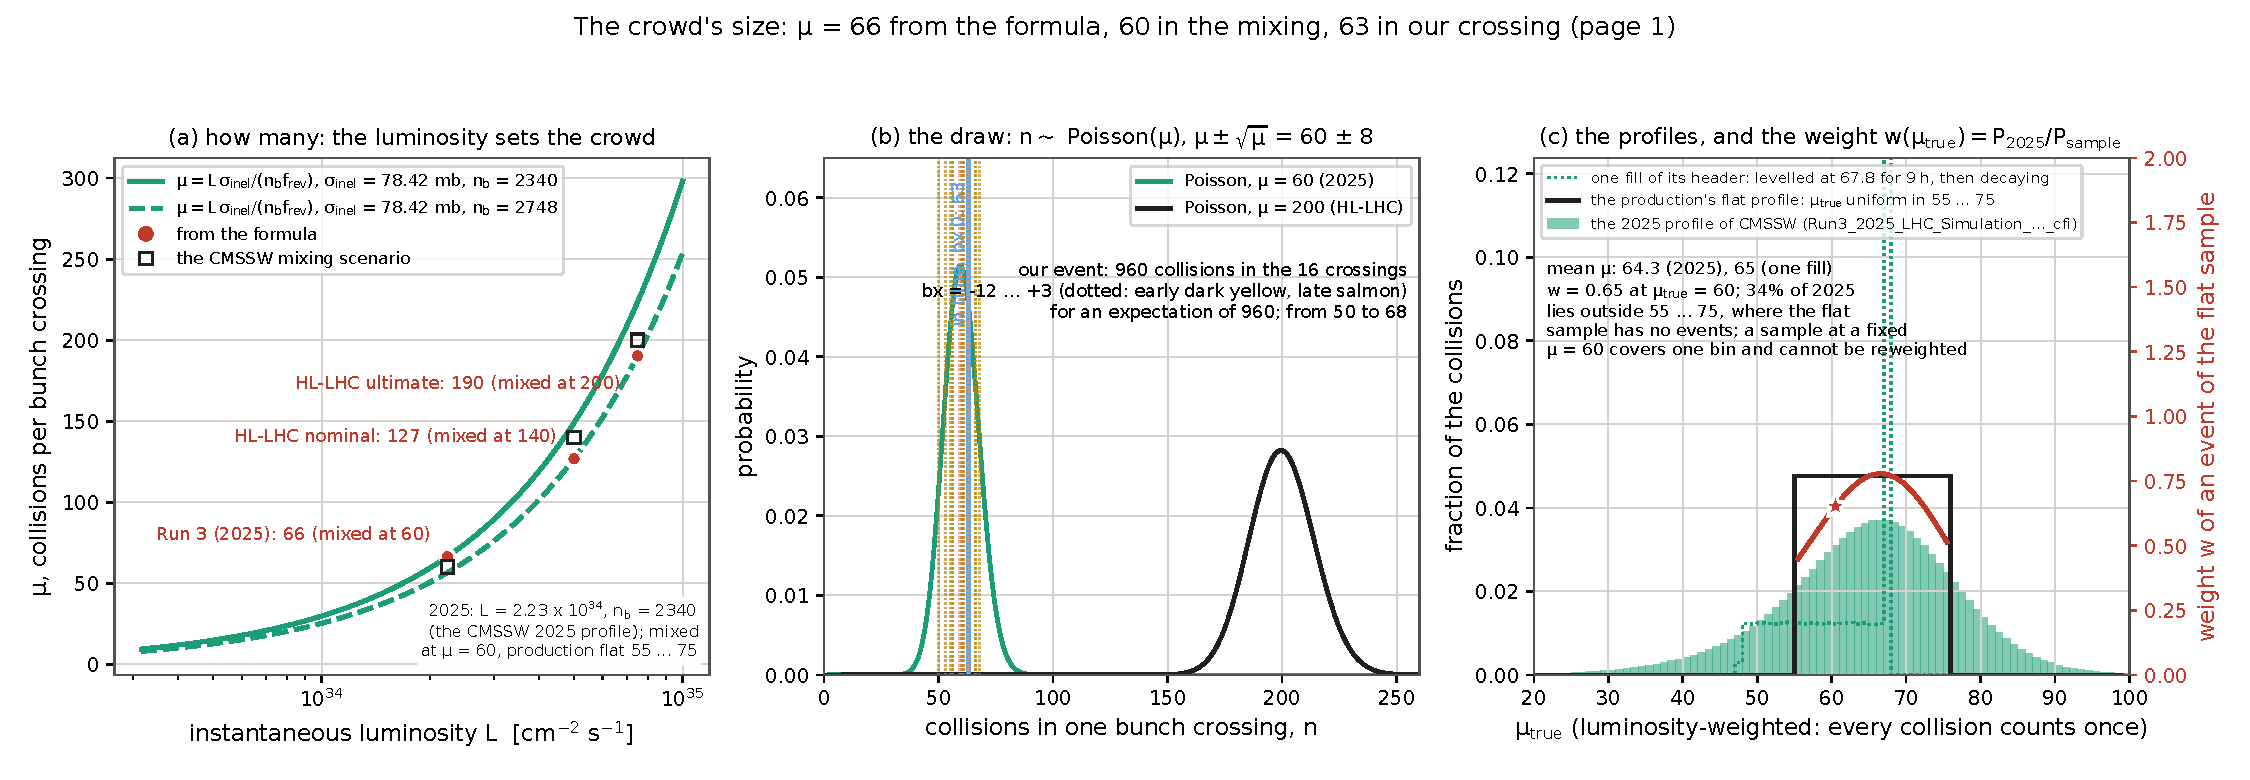
\includegraphics[page=1,width=\textwidth]{PU/Standalone/theory_pileup.pdf}
\caption[The crowd's size: $\mup$ against the luminosity, the Poisson draw,
the profiles]{Page~1 of \file{theory_pileup.pdf}. (a)
\Cref{eq:crowd_on_the_road:mu} against the luminosity, with the three
scenarios from the formula and the values \CMSSW mixes at. (b) The Poisson
distributions of $\mup=60$ and $200$, and the sixteen draws of our event,
one per crossing. (c) The pileup profile of a 2024-like year of levelled
fills, one fill, the flat $55$--$75$ profile of the Run-3 production, and
the weight of \cref{eq:crowd_on_the_road:reweight} for an event of the
flat sample.}
\label{fig:crowd_on_the_road:theory_mu}
\end{figure}

\subsection{One member of the crowd: the minimum-bias collision}
\label{sec:crowd_on_the_road:one_member}

What does one of the sixty carry? Not a hard scattering: a collision with
a $100\GeV$ parton pair in it is one in a hundred thousand, and the crowd
is what happens in all the others, the inelastic collisions in their
natural proportions, which the experiments call \emph{minimum bias} after
the trigger that selects them with the least possible bias. \PYTHIA makes
them as \code{SoftQCD:inelastic}, the sum of the four processes of
\cref{fig:crowd_on_the_road:minbias_sketch}: the non-diffractive
collision, in which both protons break up and several parton pairs
interact as in \cref{ch:uninvited_cousins}, so that the plateau of soft
particles stretches over ten units of rapidity; the single-diffractive
one, in which one proton survives and the other dissociates, leaving a
gap in rapidity on the surviving side; the double-diffractive one, both
dissociating with a gap between them; and the central-diffractive one,
both surviving and a small system in the middle. Their cross sections are
not computed from the parton distributions: the CP5 tune fixes the total
and the elastic cross sections, $\sigma_{\mathrm{tot}}=100.31$ and
$\sigma_{\mathrm{el}}=21.89\mbarn$, at whatever energy it is run, the
diffractive pieces come from \PYTHIA's parametrisation and the
non-diffractive part is what remains,
\begin{equation}
  \sigmainel=\sigma_{\mathrm{tot}}-\sigma_{\mathrm{el}}=78.42\mbarn
  =\underbrace{55.42}_{\mathrm{ND}}+\underbrace{2\times6.43}_{\mathrm{SD}}+\underbrace{8.85}_{\mathrm{DD}}+\underbrace{1.29}_{\mathrm{CD}}\ \mbarn,
  \label{eq:crowd_on_the_road:sigma}
\end{equation}
the shares $70.7$, $16.4$, $11.3$ and $1.6\%$, which the library
reproduces as $71.2$, $16.0$, $11.0$ and $1.9$ in its two thousand
collisions and the $250$-event \CMSSW library as $183$, $45$, $19$ and
$3$. The $14\TeV$ fragment of the release gives the same numbers to the
second decimal, which is why the Run-3 workflows can mix their
$13.6\TeV$ signals with a $14\TeV$ library and why the companion sets the
energy by hand instead. The measured inelastic cross section at $13\TeV$
is $79.5\pm1.8\mbarn$~\cite{ATLAS:2016ygv,CMS:2018mlc}, and the $80\mbarn$
of the bookkeeping is that number rounded.

\begin{figure}[htbp]\centering
\resizebox{\textwidth}{!}{% ---------------------------------------------------------------------------
% One member of the crowd: the four inelastic process types of SoftQCD:inelastic
% with their rapidity profiles (ND: both protons break up, a plateau; SD: one
% proton survives, a gap; DD: both dissociate, a gap in the middle; CD: both
% survive, a small central system), their cross sections and their shares in
% the 2000-event library of make_pileup_library.py (13.6 TeV).
% ---------------------------------------------------------------------------
\begin{tikzpicture}[x=1cm,y=1cm,
  every node/.style={font=\footnotesize},
  lab/.style={font=\scriptsize,align=center},
  head/.style={font=\small\bfseries},
  prot/.style={-{Stealth[length=2mm]},thick},
  prof/.style={thick}]
\foreach \dx/\name/\col/\code/\sig/\share/\np/\desc in {
   0/ND/blue!60!black/101/55.4 mb/71.2\%/230/{both protons break up; several parton pairs interact (MPI); a plateau of $\sim6$ charged per unit of $\eta$},
   5.2/SD/green!50!black/103+104/12.9 mb/15.9\%/51/{one proton survives intact, the other dissociates; a rapidity gap on the surviving side},
   10.4/DD/orange!80!black/105/8.8 mb/10.9\%/62/{both dissociate into low-mass systems; a gap in the middle, little in the tracker},
   15.6/CD/violet!80!black/106/1.3 mb/1.9\%/28/{both survive; a small system in the centre: a few particles}} {
 \begin{scope}[xshift=\dx cm]
  \node[head,anchor=west,text=\col] at (-0.2,3.3) {\name\quad\textcolor{black!60}{code \code}};
  % the eta axis
  \draw[-{Stealth}] (-0.2,0) -- (4.4,0) node[below left,lab] {$\eta$};
  \foreach \x/\t in {0.4/$-8$,1.3/$-4$,2.1/0,2.9/4,3.8/8} {\draw (\x,-0.05) -- (\x,0.05); \node[lab,anchor=north] at (\x,-0.08) {\t};}
  \draw[black!30] (1.6,0) -- (1.6,1.9); \draw[black!30] (2.6,0) -- (2.6,1.9);
  \node[lab,text=black!50] at (2.1,2.0) {tracker};
  \draw[black!15,dashed] (1.1,0) -- (1.1,1.9); \draw[black!15,dashed] (3.1,0) -- (3.1,1.9);
 \end{scope}
}
% the profiles, hand drawn: dN/deta per unit eta (scale 0.2 cm per particle)
\begin{scope}
 \draw[prof,blue!60!black] plot[smooth] coordinates {(0.3,0.1)(0.7,0.9)(1.1,1.3)(1.5,1.4)(2.1,1.45)(2.7,1.4)(3.1,1.3)(3.5,0.9)(3.9,0.1)};
 \node[lab,text=blue!60!black] at (2.1,1.7) {$\sim6$ charged per unit $\eta$};
\end{scope}
\begin{scope}[xshift=5.2cm]
 \draw[prof,green!50!black] plot[smooth] coordinates {(0.3,0.1)(0.7,0.8)(1.1,1.0)(1.4,0.9)(1.7,0.5)(1.9,0.15)(2.2,0.05)(3.9,0.05)};
 \draw[prot,green!50!black] (3.9,0.6) -- (4.3,0.6); \node[lab,text=green!50!black,anchor=south] at (4.0,0.65) {$p$};
 \node[lab,text=green!50!black] at (3.0,0.5) {gap};
\end{scope}
\begin{scope}[xshift=10.4cm]
 \draw[prof,orange!80!black] plot[smooth] coordinates {(0.3,0.1)(0.7,0.8)(1.0,0.9)(1.3,0.5)(1.6,0.1)(2.6,0.1)(2.9,0.5)(3.2,0.9)(3.5,0.8)(3.9,0.1)};
 \node[lab,text=orange!80!black] at (2.1,0.5) {gap};
\end{scope}
\begin{scope}[xshift=15.6cm]
 \draw[prof,violet!80!black] plot[smooth] coordinates {(0.3,0.03)(1.5,0.05)(1.9,0.4)(2.1,0.5)(2.3,0.4)(2.7,0.05)(3.9,0.03)};
 \draw[prot,violet!80!black] (3.9,0.6) -- (4.3,0.6); \draw[prot,violet!80!black] (0.3,0.6) -- (-0.1,0.6);
 \node[lab,text=violet!80!black,anchor=south] at (4.0,0.65) {$p$}; \node[lab,text=violet!80!black,anchor=south] at (0.2,0.65) {$p$};
\end{scope}
% the table below each
\foreach \dx/\col/\sig/\share/\np/\nc/\desc in {
   0/blue!60!black/55.4 mb/71.2\%/230/16/{both protons break up; several parton pairs interact (MPI); a plateau},
   5.2/green!50!black/12.9 mb/15.9\%/51/3/{one proton survives, the other dissociates; a gap on the surviving side},
   10.4/orange!80!black/8.8 mb/10.9\%/62/3/{both dissociate into low-mass systems; a gap in the middle, little in the tracker},
   15.6/violet!80!black/1.3 mb/1.9\%/28/2/{both survive; a small system in the centre, a few particles}} {
  \node[lab,anchor=north west,text width=4.5cm,align=left] at (\dx cm-0.2cm,-0.55) {\textcolor{\col}{$\sigma=\sig$, \share\ of the library}\\ \np\ particles on average, \nc\ charged in the tracker\\ \desc};
}
\node[lab,anchor=north west,text width=20cm,align=left] at (-0.2,-2.5) {\textbf{Minimum bias} is all of them in their natural proportions, $\sigma_{\rm inel}=78.4$ mb at 13.6 TeV (\PYTHIA, CP5: $\sigma_{\rm tot}=100.3$ and $\sigma_{\rm el}=21.9$ mb fixed by the tune, the same at 14 TeV; the diffractive pieces from its parametrisation, ND what remains). The library holds 2000 of them: 179 final particles per collision on average, a median of 116, from 3 to 829; the hardest particle $2.2$ GeV on average; $0.95$ GeV of $p_T$ per unit area in the tracker's reach.};
\end{tikzpicture}
}
\caption[One member of the crowd: the four kinds of inelastic collision]{One
member of the crowd. The four processes of \code{SoftQCD:inelastic} with
their profiles in rapidity, their cross sections at $13.6\TeV$, their
shares in the library of two thousand collisions and the particles each
brings on average.}
\label{fig:crowd_on_the_road:minbias_sketch}
\end{figure}

\Cref{tab:crowd_on_the_road:catalogue} is the crowd one member at a
time, the catalogue of the library as the companion's
\code{minBiasGenStats.py} prints it for the $250$ GEN events of the 2024
\CMSSW library: the first ten collisions of our in-time crossing, each
with its kind, its parton-parton interactions, its particles, what the
tracker and what nothing will see of them, its hardest particle, its
jets, its forward protons, and the vertex the mixing drew for it. The
first of the ten is a single-diffractive collision of four particles,
a surviving proton among them, that no central detector will notice; the
eighth is a non-diffractive one with $24$ interactions and $537$
particles, $93$ of them in the tracker's reach, more than the family's
own $93$. The summary below it, over the two thousand, and the means per
kind say the rest.

\begin{table}[htbp]\centering\small
\caption[The catalogue of the library: ten collisions, the summary and
the means per kind]{The catalogue of the library, written by
\file{minbias_catalogue.py} in the format of the companion's
\code{minBiasGenStats.py}. Top: the first ten in-time collisions of our
crossing, with their library event, kind, parton-parton interactions
(the hardest scattering plus the multiparton ones), stable particles,
charged ones, central ones ($|\eta|<2.5$ and $\pt>0.5\GeV$, all species),
the ones beyond $|\eta|=5.5$ where no subdetector is, the hardest
particle, the scalar sum of \pt, the \antikt $R=0.4$ jets above
$10\GeV$, the forward protons that keep most of the beam energy
($\xi<0.55$, the ones \CMSSW's \code{LHCTransport} carries to the PPS),
and the vertex the mixing drew. Middle: the same quantities over the two
thousand collisions of the library, with the vertices of the $960$
collisions of our event. Bottom: the means per kind, with the cross
section of each at $13.6\TeV$.}
\label{tab:crowd_on_the_road:catalogue}
\scriptsize\setlength{\tabcolsep}{3pt}
\resizebox{\textwidth}{!}{\minbiasCatalogueTen}\\[2mm]
\minbiasCatalogueSummary\\[2mm]
\resizebox{\textwidth}{!}{\minbiasCataloguePerProcess}
\end{table}

A member of the crowd, then, is soft and uneven. The library's
collisions have from $3$ to $829$ final particles, $179$ on average and a
median of $116$: a non-diffractive one brings $230$ particles and $16$
charged ones into the tracker's reach, $|\eta|<2.5$ and $\pt>0.5\GeV$, a
diffractive one $50$ to $60$ and $3$, a central-diffractive one $28$ and
$2$; the hardest particle of a collision is $2.2\GeV$ on average, and in
two thousand collisions it never exceeded $18$. Where they walk is the
plateau: $5.5$ charged particles per unit of pseudorapidity at $\eta=0$,
$13$ with the neutrals, falling off beyond the tracker and gone beyond
$|\eta|=8$, where the beam remnants carry the rest of the energy into the
beam pipe. What they carry is the number this chapter is about. The
transverse momentum of a collision per unit of $\eta$ and $\phi$,
\begin{equation}
  \rhoPU_1=\frac{1}{2\pi}\,\Big\langle\frac{\mathrm{d}\Sigma\pt}{\mathrm{d}\eta}\Big\rangle_{\text{one collision}}
  =0.95\GeV\ \text{per unit area at }|\eta|<2.5,
  \label{eq:crowd_on_the_road:rho1}
\end{equation}
averaged over the library without the neutrinos, is the slope of
everything that follows: sixty collisions put $57\GeV$ into every unit of
area, and a jet of $R=0.4$ covers $\pi R^2=0.503$ of them, $29\GeV$
under our $100\GeV$ jet before any subtraction.
\Cref{fig:crowd_on_the_road:theory_member} shows the three panels, and
the one surprise in them: the multiplicity distribution is so wide that
the median collision has two thirds of the mean, and in any crossing a
handful of the sixty, the non-diffractive ones with many multiparton
interactions, carry a quarter of the crowd. The \CMSSW library of the
companion, $250$ collisions through the full chain, has $194$ stable
particles per collision with a median of $132$, from $3$ to $723$, and
the same shape; ten of its events, single-diffractive ones that hand
\GEANT a surviving proton and nothing else, leave no hit in the central
detector at all.

\begin{figure}[htbp]\centering
\includegraphics[page=2,width=\textwidth]{PU/Standalone/theory_pileup.pdf}
\caption[One member of the crowd: the multiplicity, the plateau, the
transverse momentum per unit area]{Page~2 of \file{theory_pileup.pdf}.
(a) The final particles per collision in the library, by process type,
with the \CMSSW library's mean and our signal event for comparison. (b)
The particles per unit of $\eta$ per collision, all and charged: the
plateau, the tracker's reach and the beam remnants. (c) The transverse
momentum per unit area per collision, \cref{eq:crowd_on_the_road:rho1},
and the slope of \rhoPU it predicts against the one measured over four
hundred draws.}
\label{fig:crowd_on_the_road:theory_member}
\end{figure}

\subsection{Where and when: the beam spot and the 25 ns clock}
\label{sec:crowd_on_the_road:in_time_out_of_time_and_the_25_ns_bunch_}

The crowd walks in the same picture, but not from the same point. Two
bunches of protons pass through each other, and a collision can happen
anywhere in their overlap and at any moment of it; the region where the
collisions happen, the \emph{beam spot}, is what the vertex finder of
\cref{ch:first_checkpoint} will use to tell the crowd from the family, and
its time spread is what no detector of Run~3 can resolve.
\Cref{fig:crowd_on_the_road:region_sketch} draws it. Bunch~1 moves along
$+z$ and bunch~2 along $-z$; at the laboratory time $t$ their centres are
at $z=\pm ct$, and a proton at the longitudinal offset $s$ from its bunch
centre sits at $z=\pm ct+s$. For two Gaussian bunches of length
$\sigma_s$ meeting head-on the density of collisions is the product of
the two bunch densities at the same point and time,
\begin{equation}
  p(z,t)\propto
  \exp\!\Big[-\frac{(z-ct)^2+(z+ct)^2}{2\sigma_s^2}\Big]
  =\exp\!\Big[-\frac{z^2}{2\sigma_z^2}\Big]\exp\!\Big[-\frac{t^2}{2\sigma_t^2}\Big],
  \qquad \sigma_z=\frac{\sigma_s}{\sqrt2},\quad \sigma_t=\frac{\sigma_z}{c},
  \label{eq:crowd_on_the_road:region}
\end{equation}
after the transverse coordinates have been integrated out: a Gaussian
along the beam, a Gaussian in time of the same width in units of $z/c$,
and the two independent, because the cross term $z\,ct$ cancels between
the two bunches. Across the beam the collisions follow the beam size,
$\sigma_{x,y}(z)=\sqrt{\epsilon\beta^*/2}\,\sqrt{1+(z-z_0)^2/\beta^{*2}}$,
narrowest at the focus and growing on either side, the hourglass of a
beam focused to $\beta^*$. This is exactly the model of \CMSSW's
\code{BetafuncEvtVtxGenerator}, the \code{VtxSmeared} of every Run-3
GEN step: it draws $z$ and $t$ as independent Gaussians of the same
width, and $x$ and $y$ around the centre of the beam spot with the
hourglass width at that $z$. What it does not do is compute $\sigma_z$
from the bunches. The real bunches of Run~3 are longer than
$\sqrt2\times3.6\cm$ and cross at an angle, which shortens their overlap,
and the generator reads instead the \emph{measured} beam spot from the
database, the \code{SimBeamSpot} payload of the 2024 global tag, a fit to
the early-2024 data: centre $(0.03,-0.02,0.42)\cm$, $\sigma_z=3.6\cm$,
$\beta^*=30\cm$ and an emittance of $5.7\times10^{-8}\cm$, hence
$\sigma_t=120\ps$ and $\sigma_{xy}=9\um$ at the focus. The script draws
every vertex of the crowd, and the signal's, from that payload: the $960$
vertices of our event have an r.m.s.\ of $3.79\cm$ in $z$ and $119\ps$
in $t$, $9\um$ across, and the signal sits at $z=-0.17\cm$, $t=-121\ps$.
The $250$-event \CMSSW library of the companion, drawn by the real
module, has $3.56\cm$ and $122\ps$ with its vertices between $-9.5$ and
$+10.1\cm$, and the \CMSSW signal event sits at $z=3.11\cm$. The HL-LHC
of the open problems is another story: there the crossing angle would
cut the overlap to $2\cm$, crab cavities give most of it back, and
\CMSSW's \code{HLLHCEvtVtxGenerator} builds the region from the bunches,
$4.3\cm$ and $190\ps$; the script keeps that model as \code{--region
hllhc}.

\begin{figure}[htbp]\centering
\resizebox{\textwidth}{!}{% ---------------------------------------------------------------------------
% The beam spot of 2025: (a) the two bunches in the (x, z) plane and their
% overlap, with the hourglass of the beta function; (b) the numbers of the
% payload against the drawn vertices, the CMSSW library and the HL-LHC model;
% the clock of the sixteen crossings is pu_clock.tex.
% ---------------------------------------------------------------------------
\begin{tikzpicture}[x=1cm,y=1cm,
  every node/.style={font=\footnotesize},
  lab/.style={font=\scriptsize,align=center},
  head/.style={font=\small\bfseries}]
% ---------------- (a) the crossing plane --------------------------------------------------------------
\begin{scope}
\node[head,anchor=west] at (-0.3,3.4) {(a) the beam spot in the $(x,z)$ plane};
\draw[-{Stealth}] (-4.2,0) -- (4.4,0) node[below left,lab] {$z$};
\draw[-{Stealth}] (0,-1.6) -- (0,2.2) node[left,lab] {$x$ ($\times10^{3}$)};
% the hourglass envelope: sigma(z) = sigma0 sqrt(1 + z^2/beta*^2), beta* = 30 cm (scale 0.2 cm per cm)
\draw[black!35,dashed] plot[domain=-4:4,samples=60] (\x,{0.22*sqrt(1+(\x/1.2)*(\x/1.2))});
\draw[black!35,dashed] plot[domain=-4:4,samples=60] (\x,{-0.22*sqrt(1+(\x/1.2)*(\x/1.2))});
\node[lab,text=black!50,anchor=west] at (-4.1,1.7) {hourglass: $\sigma_x(z)=\sigma_{x0}\sqrt{1+(z-z_0)^2/\beta^{*2}}$, $\beta^*=30$ cm};
% bunch 1 (blue) moving +z, bunch 2 (orange) moving -z, a small crossing angle
\begin{scope}[rotate=5]
 \fill[blue!25,opacity=0.8] (-1.9,0) ellipse (1.8 and 0.22);
\end{scope}
\begin{scope}[rotate=-5]
 \fill[orange!35,opacity=0.8] (1.9,0) ellipse (1.8 and 0.22);
\end{scope}
\draw[blue!60!black,thick,-{Stealth[length=2mm]}] (-3.6,-0.75) -- (-2.6,-0.6) node[lab,below,pos=0.3] {bunch 1};
\draw[orange!80!black,thick,-{Stealth[length=2mm]}] (3.6,-0.75) -- (2.6,-0.6) node[lab,below,pos=0.3] {bunch 2};
\fill[green!50!black,opacity=0.55] (0.1,0) ellipse (0.72 and 0.16);
\node[lab,text=green!50!black,anchor=north] at (0.1,-0.25) {the overlap: $\sigma_z=3.6$ cm, $\sigma_t=120$ ps, $\sigma_{xy}=9\,\mu$m};
\node[lab,anchor=north west,text width=8.8cm,align=left] at (-4.2,-1.85) {Two Gaussian bunches meeting head-on collide over $\sigma_z=\sigma_s/\sqrt2$, during $\sigma_t=\sigma_z/c$, with $z$ and $t$ independent, \cref{eq:crowd_on_the_road:region}. The crossing angle of Run 3 shortens the overlap; \CMSSW does not model it but reads the measured region from the database: \code{BetafuncEvtVtxGenerator} draws $z$, $t$, $x$ and $y$ from the 2025 payload, the signal and every library event alike.};
\end{scope}
% ---------------- (b) the numbers --------------------------------------------------------------------
\begin{scope}[xshift=12.4cm]
\node[head,anchor=west] at (-3.2,3.4) {(b) how long, how wide: the payload and three checks};
\foreach \y/\t/\v/\w in {2.6/{the 2025 payload}/3.60/2.88, 1.9/{our 960 vertices}/3.56/2.85, 1.2/{\CMSSW library (1000)}/3.57/2.86, 0.5/{the HL-LHC model}/4.27/3.42} {
  \draw[fill=green!30] (0,\y-0.18) rectangle (\w,\y+0.18);
  \node[lab,anchor=west] at (\w+0.1,\y) {\v\ cm};
  \node[lab,anchor=east] at (-0.1,\y) {\t};
}
\draw[-{Stealth}] (0,0.1) -- (4.3,0.1) node[below left,lab] {$\sigma_z$ [cm], 0.8 cm per cm};
\node[lab,anchor=north west,text width=7.6cm,align=left] at (-3.2,-0.5) {In time the same four read $120$, $124$, $122$ and $193$ ps. The payload of the 2025 global tag is a fit to early-2024 data: centre $(0.03,-0.02,0.42)$ cm, $\sigma_z=3.6$ cm, $\beta^*=30$ cm, emittance $5.7\times10^{-8}$ cm, hence $\sigma_{xy}=\sqrt{\epsilon\beta^*/2}=9\,\mu$m at the focus. The HL-LHC region is longer because the crab cavities give back what its larger crossing angle takes.};
\end{scope}
\end{tikzpicture}
}
\caption[The beam spot of 2024: the two bunches and the numbers of the
payload]{The beam spot. (a) The $(x,z)$ plane: the two bunches, their
overlap and the hourglass of the $\beta$ function. (b) The length of the
beam spot: the 2024 payload against the vertices of our event, the
\CMSSW library and the HL-LHC model.}
\label{fig:crowd_on_the_road:region_sketch}
\end{figure}

The clock is the other half, and \cref{fig:crowd_on_the_road:clock}
draws it with the numbers of our event. The crossings before and after
ours, $25\ns$ apart, collide on the same beam spot, and their collisions
are the same crowd shifted in time: the \Mix draws each of the sixteen
crossings of the production window on its own, $60$, $56$, $68$, $61$,
$66$, $56$, $55$, $50$, $53$, $66$, $61$ and $60$ collisions in the
twelve early ones, $63$ in ours, $63$, $59$ and $63$ in the three late
ones, $960$ collisions piled on one signal event, of which $712$ arrive
early, up to $300\ns$ before the signal, and $185$ late, up to $75\ns$
after it. \CMSSW's \code{Adjuster} stamps every \code{SimTrack},
\code{SimVertex} and hit of collision $k$ of crossing \bx with
\code{EncodedEventId(bx, k)} and adds $25\ns\times\bx$ to its time, so
that in the simulation, and only there, the question ``which crowd did
this come from'' has an answer: \code{bunchCrossing() = 0} with
\code{event() = 0} is the signal, \code{bunchCrossing() = 0} with
\code{event()} of one or more is an in-time collision, and anything with
\code{bunchCrossing()} different from zero is out of time; the
\code{TrackingParticle}s and the \code{DigiSimLink}s carry the id
through the digitisation, which is how the companion's pages colour
every hit by its crowd and how a reconstructed track can be called
signal, in-time or out-of-time pileup in a validation. The record of
this stop keeps the same two numbers, \bx and $k$, in its vertex listing
for the $897$ out-of-time collisions and for the $63$ in-time ones. In
space nothing distinguishes an early collision from an in-time one, which
is why the tracker, which does not keep time to a nanosecond, cannot; the
calorimeter pulses of \cref{ch:first_checkpoint}, which last several
crossings, will integrate them, and the price of that is the out-of-time
pileup of the chapters ahead. At the generator level nothing integrates
over $25\ns$, so the particles of the other crossings are not clustered
here; they are in the record for \cref{ch:crossing_the_border}. What the
in-time crowd does to
the vertex finder, on the other hand, can be counted now. A collision the
tracker can see needs charged particles above its threshold pointing back
to a common point, and with the proxy of at least four charged particles
of $\pt>0.5\GeV$ within $|\eta|<2.5$, $43$ of the $63$ collisions of our
crossing are visible, $62\%$ over the ensemble, against the $0.7\mup$ that
CMS reconstructs with its real threshold; the rest are diffractive or
forward and leave the tracker empty. Their vertices are a Gaussian of
$3.6\cm$ with sixty entries, so the typical spacing is a millimetre: the
nearest crowd vertex to ours is $0.06\,\mathrm{mm}$ away in $z$ in our
crossing and $0.98$ on the median of the ensemble, in one draw of two one
of them is within a millimetre, and the vertex finder, which resolves
vertices a few hundred microns apart, will merge the two in a fair
fraction of the events; the \CMSSW event of the companion has three
pileup vertices within a millimetre of the signal's. In time the nearest
is five picoseconds away and nine of them are within $30\ps$ on average,
which is the number a timing layer would sort by; Run~3 has none, and in
this book the time of a collision is a label the record carries and no
detector reads. \Cref{fig:crowd_on_the_road:theory_region} draws the
density, the length of the beam spot three ways and the clock.

\begin{figure}[htbp]\centering
\resizebox{\textwidth}{!}{% ---------------------------------------------------------------------------
% The clock: the sixteen crossings of the Run-3 production window, 25 ns
% apart, with the number of collisions the MixingModule drew for each in our
% event (the -v log, seed 1), the in-time crossing with the signal, and the
% EncodedEventId(bx, k) that lets the simulation tell them apart.
% ---------------------------------------------------------------------------
\begin{tikzpicture}[x=1cm,y=1cm,
  every node/.style={font=\footnotesize},
  lab/.style={font=\scriptsize,align=center},
  head/.style={font=\small\bfseries}]
\node[head,anchor=west] at (-0.6,3.6) {the window $bx=-12\ldots+3$: sixteen crossings, sixteen Poisson draws, 960 collisions on one signal event};
\draw[-{Stealth}] (-0.6,0) -- (17.2,0) node[below left,lab] {$t$ [ns]};
% bars: height 0.04 cm per collision (60 -> 2.4 cm)
\foreach \bx/\n/\col in {-12/60/yellow!60!brown,-11/56/yellow!60!brown,-10/68/yellow!60!brown,-9/61/yellow!60!brown,-8/66/yellow!60!brown,-7/56/yellow!60!brown,-6/55/yellow!60!brown,-5/50/yellow!60!brown,-4/53/yellow!60!brown,-3/66/yellow!60!brown,-2/61/yellow!60!brown,-1/60/yellow!60!brown,0/63/cyan!60!blue,1/63/red!50!orange,2/59/red!50!orange,3/63/red!50!orange} {
  \pgfmathsetmacro{\x}{12.6+1.0*\bx}
  \pgfmathsetmacro{\h}{0.04*\n}
  \fill[\col,opacity=0.75] (\x-0.32,0) rectangle (\x+0.32,\h);
  \node[lab,anchor=south] at (\x,\h+0.02) {\n};
  \node[lab,anchor=north] at (\x,-0.06) {$\bx$};
}
\foreach \bx in {-12,-8,-4,0,3} {\pgfmathsetmacro{\x}{12.6+1.0*\bx} \node[lab,anchor=north,text=black!60] at (\x,-0.42) {$25\times(\bx)$};}
\draw[black!40,dashed] (-0.6,2.4) -- (16.4,2.4) node[lab,anchor=west,text=black!60] at (16.45,2.4) {$\mu=60$};
\node[star,star points=5,fill=red!80!black,inner sep=0pt,minimum size=9pt] at (12.6,1.2) {};
\node[lab,text=red!80!black,anchor=west] at (12.85,1.25) {ours};
\node[lab,anchor=north west,text width=5.2cm,align=left,text=yellow!50!brown] at (-0.6,-0.95) {\textbf{early}, $bx<0$: 12 crossings, 712 collisions; their hits arrive $25\,{\rm ns}\times|bx|$ before the signal, up to 300 ns, and the slow detectors (calorimeter pulses, strip readout) remember them};
\node[lab,anchor=north west,text width=4.6cm,align=left,text=cyan!50!blue] at (5.4,-0.95) {\textbf{in time}, $bx=0$: 63 collisions in the same crossing as the signal, 9033 particles in the detector's reach; the only ones a generator-level jet can see};
\node[lab,anchor=north west,text width=4.6cm,align=left,text=red!50!orange] at (10.6,-0.95) {\textbf{late}, $bx>0$: 3 crossings, 185 collisions, up to 75 ns after the signal: the tails of the latest pulses};
\node[lab,anchor=north west,text width=17.6cm,align=left] at (-0.6,-2.75) {In space the sixteen crowds sit on the same beam spot; only the clock tells them apart, and in the simulation the clock is written down: the \code{Adjuster} of the \code{MixingModule} stamps every \code{SimTrack}, \code{SimVertex} and hit of collision $k$ of crossing $bx$ with \code{EncodedEventId(bx, k)} and adds $25\,{\rm ns}\times bx$ to its time. \code{bunchCrossing() = 0} and \code{event() = 0} is the signal; \code{bunchCrossing() = 0} and \code{event() $\ge$ 1} an in-time pileup collision; \code{bunchCrossing() $\neq$ 0} an out-of-time one. The record of this stop keeps the same two numbers in its vertex listing ($bx$ and $k$), and the reconstruction of \cref{ch:first_checkpoint} will never see them: the truth of which hit came from which crowd exists in the simulation and nowhere else.};
\end{tikzpicture}
}
\caption[The clock: the sixteen crossings of the production window and
the collisions of each]{The clock. The sixteen crossings of the Run-3
production window, $25\ns$ apart, with the number of collisions the
\Mix drew for each in our event: $712$ early, $63$ in time with the
signal, $185$ late, $960$ in all; and the \code{EncodedEventId} by which
the simulation, and nothing after it, knows which crowd a hit came
from.}
\label{fig:crowd_on_the_road:clock}
\end{figure}

\begin{figure}[htbp]\centering
\includegraphics[page=3,width=\textwidth]{PU/Standalone/theory_pileup.pdf}
\caption[The beam spot: the density in $(z,t)$, the $z$ of the vertices,
the sixteen crossings]{Page~3 of \file{theory_pileup.pdf}. (a) The
collision density of \cref{eq:crowd_on_the_road:region} in $(z,t)$ with
the $63$ in-time collisions of our crossing and the signal. (b) The $z$
of the $960$ vertices of the event against the Gaussian of the payload
and the $250$ vertices of the \CMSSW library. (c) The sixteen crossings
on the clock, $25\ns$ apart, early in dark yellow, in time in blue and
late in salmon, the colours of the \CMSSW pages of the companion.}
\label{fig:crowd_on_the_road:theory_region}
\end{figure}

\paragraph{How \CMSSW does it: the library, the mixing and the premixing.}
\label{sec:crowd_on_the_road:how_cms_mixes_pileup_into_simulation_the}
What the script does with four-vectors, \CMSSW does with the hits of
\GEANT, and the strategy is the same. \GEANT is the expensive step,
$2.5$ seconds per minimum-bias collision, and the hits it leaves add: a
sensor crossed by particles of two collisions holds two hits, a
calorimeter cell the sum of two energies. So the minimum-bias collisions
are generated and simulated once, with the same fragment, the same vertex
smearing, the same geometry and the same \GEANT as the signal, but with
their own random seeds, and stored in a GEN-SIM library; the \Mix of the
DIGI step draws the number of collisions per crossing, reads that many
library events, stamps and shifts them, and hands the signal and the
pileup hits together to the digitisers, which add them channel by
channel and apply the pulse shapes, the time windows and the thresholds
in which the out-of-time pileup does its damage. The truth survives as
the \code{PileupSummaryInfo}, the \code{TrackingParticle}s with their
event ids, and the \code{DigiSimLink}s that say which collision
contributed what to each channel. The companion's exercise does exactly
this for one signal event, $\mup=60$ in three crossings, $66$, $55$ and
$77$ collisions drawn in sequence from a library of $250$: the $198$
collisions bring $31\,597$ primaries against the $571$ of the signal,
$444\,535$ tracker hits against $9776$, and own $104\,277$ of the
$106\,581$ hit cells of the ECAL. In the production window of sixteen
crossings this classical mixing would read a thousand library events, a
quarter of a gigabyte, per signal event, and the production therefore
\emph{premixes}~\cite{Hildreth:2017caz}: the minimum-bias events are
mixed among themselves at the flat profile and digitised once into a
library of premixed crossings, and a single premixed event is added, in
ADC counts, to every digitised signal event. The physics is the same,
the bookkeeping is a thousand times lighter, and the price is that the
pileup hits are gone from a premixed sample, so that pictures like those
of the companion, which colour every hit by the crossing it came from,
can only be drawn with the classical mixing; the script reproduces the
conditions of the exercise at the generator level with \code{--window 1
--sequential}.

\subsection{\rhoPU, the median energy density, and the jet area $A$}
\label{sec:crowd_on_the_road:rho_the_median_energy_density_and_the_je}

The crowd is uniform on average, and that is the handle. If every unit of
area of the $(\eta,\phi)$ plane receives \rhoPU GeV of transverse momentum
from the crowd, then a jet of area $A$ receives $\rhoPU A$, and
subtracting it is a matter of measuring \rhoPU in the parts of the plane
where nothing else is and $A$ for the jet. Both ideas are Cacciari and
Salam's~\cite{Cacciari:2007fd}, and \cref{fig:crowd_on_the_road:rho_sketch}
draws them. The density is estimated as a median: cut the plane into
patches, measure the transverse momentum per unit area in each, and take
the middle value,
\begin{equation}
  \rhoPU=\operatorname*{median}_{\text{patches }i}\Big[\frac{\pt^{(i)}}{A^{(i)}}\Big],
  \label{eq:crowd_on_the_road:rho}
\end{equation}
because the median does not care about the tail. The patches that hold a
jet are the top few percent and would pull a mean up, $74$ against $68$
in our crossing, and the median ignores them as long as fewer than half
the patches are jets, which is true of any event. Two choices of patch are
in use. CMS's \code{fixedGridRhoFastjetAll}, the \rhoPU of the jet energy
corrections of \cref{ch:paying_for_uninvited}, is \FASTJET's
\code{GridMedianBackgroundEstimator} on the particles of the whole
detector: a fixed grid of $18$ by $11$ cells of $0.56\times0.57$ over
$|y|<5$, in rapidity and with $\phi$ counted from zero, as \FASTJET draws
it; the original of \cite{Cacciari:2007fd} uses the $k_T$ jets of
$R=0.4$ as patches, each with its own area, within $|y|<4.4$, since the
$k_T$ algorithm of \cref{ch:the_inn} tiles the plane with jets of
comparable area rather than finding hard cores. The script does both. The
grid gives $\rhoPU=68.28\GeV$ per unit area in our crossing, the cells
ranging from $13$ to $359$; the $k_T$ jets, $175$ of them within the
range, give $69.87$; the signal alone, the underlying event of
\cref{ch:uninvited_cousins} and nothing in most cells, gives $3.42$. Per
collision that is $1.08$ and $1.11\GeV$ per unit area in this crossing,
a crowded one, and over four hundred draws \rhoPU is $59\pm12$ with a
slope of $0.94\GeV$ per collision and an offset of $3$, the family's own
underlying event, which the median counts as crowd: the slope is the
$\rhoPU_1$ of \cref{eq:crowd_on_the_road:rho1} within the difference
between a median and a mean, the $8$ collisions of Poisson spread
account for $7\GeV$ of the $12$, and the rest is the crowd's own
unevenness, the same number of collisions bringing more or fewer
particles.

\begin{figure}[htbp]\centering
\resizebox{\textwidth}{!}{% ---------------------------------------------------------------------------
% rho and the area: (a) the (eta, phi) plane tiled in the 18 x 11 cells of
% fixedGridRhoFastjetAll, the pT per unit area of each cell as a grey level,
% the jets dark; (b) the cells sorted: the median is rho, the mean is not;
% (c) the active area of a jet: the ghosts it swallowed times 0.01.
% ---------------------------------------------------------------------------
\begin{tikzpicture}[x=1cm,y=1cm,
  every node/.style={font=\footnotesize},
  lab/.style={font=\scriptsize,align=center},
  head/.style={font=\small\bfseries},
  ghost/.style={circle,fill=black!35,inner sep=0pt,minimum size=1.8pt},
  fam/.style={circle,fill=red!80!black,inner sep=0pt,minimum size=3.6pt},
  crowd/.style={circle,fill=olive!60!brown,inner sep=0pt,minimum size=2.4pt}]
% ---------------- (a) the grid ---------------------------------------------------------------------
\begin{scope}
\node[head,anchor=west] at (-0.3,3.9) {(a) the grid: 18 $\times$ 11 cells of $0.56\times0.57$ in $|y|<5$};
\pgfmathsetseed{5}
\foreach \i in {0,...,17} {
  \foreach \j in {0,...,10} {
    \pgfmathsetmacro{\v}{min(100, 35 + 25*rnd + 15*rnd*rnd)}
    \pgfmathsetmacro{\g}{100-\v*0.6}
    \fill[black!\g] (\i*0.4,\j*0.3) rectangle (\i*0.4+0.4,\j*0.3+0.3);
  }
}
\fill[black!85] (3.2,0.6) rectangle (3.6,0.9); \fill[black!75] (2.8,0.6) rectangle (3.2,0.9);
\fill[black!85] (2.0,2.4) rectangle (2.4,2.7); \fill[black!70] (4.8,1.5) rectangle (5.2,1.8);
\draw[black!40,very thin] (0,0) grid[step=0.4] (7.2,3.3);
\draw[red!80!black,thick] (3.3,0.75) circle (0.29);
\node[lab,text=red!80!black,anchor=west] at (3.65,0.75) {our jet};
\draw[-{Stealth}] (0,-0.25) -- (7.2,-0.25) node[below left,lab] {$y$: $-5$ to $5$};
\draw[-{Stealth}] (-0.25,0) -- (-0.25,3.3) node[above,lab] {$\phi$};
\node[lab,anchor=north west,text width=7.4cm,align=left] at (-0.3,-0.65) {Every particle's $p_T$ goes to its cell; the cell's value is $\Sigma p_T/(\Delta y\,\Delta\phi)$. At $\mu=60$ a typical cell holds $\sim22$ GeV in $0.32$ units of area, 68 GeV per unit area; the cells with a jet hold up to 360.};
\end{scope}
% ---------------- (b) the median --------------------------------------------------------------------
\begin{scope}[xshift=8.6cm]
\node[head,anchor=west] at (-0.4,3.9) {(b) the 198 cells sorted: the median is $\rho$};
\draw[-{Stealth}] (0,0) -- (6.0,0) node[below left,lab] {cell, sorted by $p_T$/area};
\draw[-{Stealth}] (0,0) -- (0,3.4) node[left,lab] {GeV per unit area};
% a sorted distribution: flat-ish middle, a tail of jets at the right
\draw[olive!60!brown,very thick] plot[domain=0:5.7,samples=80] (\x,{0.25+1.2*\x/5.7+0.25*(\x/5.7)^3+2.2*exp(-(5.7-\x)*(5.7-\x)/0.25)});
\draw[red!80!black,thick,dashed] (2.85,0) -- (2.85,2.6);
\node[lab,text=red!80!black,anchor=south] at (2.85,2.65) {median: $\rho=68$};
\draw[black!60,dashed] (0,1.25) -- (5.7,1.25);
\node[lab,text=black!60,anchor=west] at (0.1,1.45) {mean, pulled up by the tail};
\node[lab,text=olive!60!brown,anchor=east] at (5.6,3.2) {the jets};
\node[lab,anchor=north west,text width=6.4cm,align=left] at (-0.4,-0.65) {$\rho=\mathrm{median}_{\rm cells}\,[\,p_T/A\,]$. The median is what the crowd puts in a cell with nothing else in it; the jets are the top few percent and do not move it. Cacciari and Salam's original uses $k_T$ jets of $R=0.4$ with their areas in place of the cells: $\rho_{\rm jets}$ a few percent above the grid ($69.9$ against $68.3$ here).};
\end{scope}
% ---------------- (c) the area ------------------------------------------------------------------------
\begin{scope}[xshift=16.2cm]
\node[head,anchor=west] at (-0.4,3.9) {(c) the active area: ghosts of $0.01$ each};
\pgfmathsetseed{3}
\foreach \i in {0,...,15} {\foreach \j in {0,...,13} {
  \pgfmathsetmacro{\xx}{0.1+0.33*\i+0.2*(rnd-0.5)}
  \pgfmathsetmacro{\yy}{0.1+0.235*\j+0.15*(rnd-0.5)}
  \node[ghost] at (\xx,\yy) {};
}}
\draw[red!80!black,thick] (2.7,1.65) circle (1.15);
\pgfmathsetseed{11}
\foreach \i in {1,...,22} {\pgfmathsetmacro{\r}{1.15*0.5*rnd*rnd} \pgfmathsetmacro{\a}{360*rnd} \node[fam] at ({2.7+\r*cos(\a)},{1.65+\r*sin(\a)}) {};}
\pgfmathsetseed{17}
\foreach \i in {1,...,40} {\pgfmathsetmacro{\xx}{0.2+5.0*rnd} \pgfmathsetmacro{\yy}{0.15+3.0*rnd} \node[crowd] at (\xx,\yy) {};}
\node[lab,anchor=north west,text width=6.0cm,align=left] at (-0.4,-0.1) {A grid of ghosts, $p_T=10^{-18}$, one per $0.01$ of the plane, is clustered with the particles. They move nothing (anti-$k_T$ never sees their $p_T$) but they are caught like any soft particle: $A=0.01\times n_{\rm ghosts}$ in the jet. For a lone hard jet $A\simeq\pi R^2=0.503$; a neighbour steals part of it. Then $p_T^{\rm sub}=p_T-\rho\,A$: the \code{L1FastJet} correction of \cref{ch:paying_for_uninvited} in its generator-level form.};
\end{scope}
\end{tikzpicture}
}
\caption[\rhoPU and the area: the grid, the median, the ghosts]{\rhoPU
and the area. (a) The $(y,\phi)$ plane tiled in the cells of
\code{fixedGridRhoFastjetAll}, the transverse momentum per unit area of
each cell as a grey level, the jets dark. (b) The cells sorted: the
median is \rhoPU, the mean is pulled up by the tail. (c) The active area
of a jet: the ghosts it swallowed, $0.01$ of the plane each, and the
subtraction $\pt-\rhoPU A$.}
\label{fig:crowd_on_the_road:rho_sketch}
\end{figure}

The area is measured with the trick of \cref{ch:family_photograph}. A
grid of ghosts, one per $0.01$ of the plane within $|y|<5$, $6300$ of
them scattered within their cells with a transverse momentum of
$10^{-18}\GeV$, is clustered together with the particles; \antikt never
sees their momentum, since the distance to a soft particle is set by the
hard one, but it catches them like any soft particle within $R$ of the
core, and the \emph{active area} of a jet is the number of ghosts it
holds times the area of one,
\begin{equation}
  A_j=0.01\times n_{\mathrm{ghosts}}(j),\qquad
  \pt^{\mathrm{sub}}=\pt-\rhoPU\,A_j,
  \label{eq:crowd_on_the_road:area}
\end{equation}
\FASTJET's \code{active\_area\_explicit\_ghosts}~\cite{Cacciari:2008gn} with
CMS's \code{GhostArea = 0.01}. A lone hard jet has $A\simeq\pi R^2=0.503$,
and our jet, whose neighbour at $\dR=0.56$ no longer competes for the
soft particles between them once the crowd fills the gap, has $0.529$;
the leading twelve jets of the crossing range from $0.49$ to $0.56$. The
subtraction is then one line, \cref{eq:crowd_on_the_road:area}, the
\code{L1FastJet} correction of \cref{ch:paying_for_uninvited} in its
generator-level form, and the script can check it against a truth the
detector never has, because every constituent of a mixed jet carries the
collision it came from: our jet reads $132.75\GeV$ with the crowd,
$\rhoPU A=68.28\times0.529=36.09$, $\pt^{\mathrm{sub}}=96.66$, and the
family's particles inside it sum to $100.07$; the crowd had put $33.61$
in, from $81$ particles of $34$ different collisions, and the subtraction
took $36.09$ out, a residual of $-3.41\GeV$. That is one draw, and the
ensemble says how typical: over four hundred draws the crowd puts
$27.8\pm8.4\GeV$ into the circle of our jet, $\rhoPU\pi R^2$ estimates
$29.7\pm5.8$, and the residual is $-1.9\pm6.7\GeV$. Two lessons are in
those three numbers. The subtraction removes the mean, and a little
more: thirty GeV of strangers become minus two, because the median
measured over the whole plane includes the family's own underlying event,
$3\GeV$ per unit area, which is signal in the truth and crowd to the
estimator; the offset corrections of \cref{ch:paying_for_uninvited}
measure and remove exactly this kind of bias. And it cannot remove the
fluctuation: the crowd inside a circle of area $0.5$ varies by $\pm8\GeV$
from crossing to crossing, the estimate $\rhoPU A$ follows only the part
of that which is common to the whole plane, and $\pm7\GeV$ remain, on a
$100\GeV$ jet whose own photograph was stable to half a GeV. This is the
first term of the jet resolution of \cref{ch:wobbly_ruler} in Run~3, and
the reason the chapters between here and there exist: a subtraction that
knows which particles came from which vertex, \cref{ch:the_police}, can
do what a density cannot. \Cref{fig:crowd_on_the_road:theory_rho} shows
the cells with their median, \rhoPU against the number of collisions, and
the truth against the estimate over the ensemble.

\begin{figure}[htbp]\centering
\includegraphics[page=4,width=\textwidth]{PU/Standalone/theory_pileup.pdf}
\caption[\rhoPU and the area: the cells and their median, \rhoPU against
the crowd, the truth against $\rhoPU A$]{Page~4 of \file{theory_pileup.pdf}.
(a) The $198$ grid cells of our crossing, their median \rhoPU and their
mean. (b) \rhoPU against the number of in-time collisions over four
hundred draws, with the slope per collision and our crossing. (c) The
pileup inside the circle of our jet against the estimate $\rhoPU\pi R^2$,
draw by draw, with the residual in the inset.}
\label{fig:crowd_on_the_road:theory_rho}
\end{figure}

\paragraph{A word on the clustering.}
Sixteen thousand pseudojets, particles and ghosts, are ten times what
\cref{ch:family_photograph} clustered, and the plain search of its
\code{Clustering} class, which revisits every pseudojet whose nearest
neighbour has just merged, slows down badly under \antikt, where the
nearest neighbour of every ghost is a hard particle, so that each merge
of a hard particle touches hundreds of ghosts. The script adds the one
idea of \FASTJET that makes the problem affordable, the tiled search: a
pair farther apart than $R$ is never merged, because $d_{ij}$ is then
larger than the beam distance of the softer of the two, which becomes a
jet first; so the nearest neighbour of a pseudojet lies within $R$ of it,
the plane is tiled in cells of side $R$, and both the search and the
update look only at the nine tiles around a pseudojet. The result is the
same, step by step; the $15\,984$ steps of our crossing take two minutes
instead of an hour, and the $33\,000$ of an HL-LHC crossing a quarter of
an hour instead of a day.

\subsubsection{The recipe, step by step}
\label{sec:crowd_on_the_road:recipe}
\Cref{fig:crowd_on_the_road:flow} is the script as a flow chart, with the
numbers of our event beside each step: the scenario and \mup, the sixteen
Poisson draws and the library, the beam spot and the vertices, the
stacking of the in-time crowd, the tiled \antikt with ghosts, the two
medians, the subtraction against the truth, the visible vertices and the
profile, and the record.

\begin{figure}[htbp]\centering
\resizebox{\textwidth}{!}{% ---------------------------------------------------------------------------
% The stage as a flow chart: the steps of standalone_pileup.py on the left,
% the numbers of our event (the -v log, seed 1, mu = 60, bx = -12 ... +3) on the right. Names
% of the classes and functions in grey.
% ---------------------------------------------------------------------------
\begin{tikzpicture}[x=1cm,y=1cm,
  every node/.style={font=\footnotesize},
  box/.style={draw,rounded corners=3pt,thick,fill=gray!8,align=left,inner sep=5pt,minimum height=10mm,text width=5.6cm},
  stepbox/.style={box,fill=orange!12},
  numbox/.style={draw,rounded corners=3pt,thin,fill=blue!6,align=left,inner sep=4pt,text width=8.6cm,font=\scriptsize},
  stepno/.style={draw,circle,inner sep=1pt,font=\scriptsize\bfseries,fill=orange!45,minimum size=5mm},
  flow/.style={-{Stealth[length=2.5mm,width=2mm]},thick},
  fn/.style={font=\scriptsize\ttfamily,text=black!65},
  head/.style={font=\small\bfseries}]
\node[head,anchor=west] at (-0.6,1.4) {the recipe};
\node[head,anchor=west] at (6.7,1.4) {our event (seed 1, $\mu=60$, $bx=-12\ldots+3$)};
\node[stepbox] (S1) at (2.5,0) {\textbf{1\; the scenario}\\ $\mu=L\sigma_{\rm inel}/(n_b f_{\rm rev})$ from the luminosity; the window of bunch crossings, 25 ns apart};
\node[stepbox,below=7mm of S1] (S2) {\textbf{2\; the draw}\\ for every crossing $n\sim{\rm Poisson}(\mu)$; the library read in order from a random position};
\node[stepbox,below=7mm of S2] (S3) {\textbf{3\; the beam spot}\\ $(x,y,z,t)$ of every collision, the signal included, from the 2025 payload: Gaussian in $z$ and $t$, the hourglass across; $+25\,{\rm ns}\times bx$};
\node[stepbox,below=7mm of S3] (S4) {\textbf{4\; the stacking}\\ one final state: the signal and the in-time collisions, $|\eta|<5$, no neutrinos; the out-of-time ones recorded, not clustered};
\node[stepbox,below=7mm of S4] (S5) {\textbf{5\; the clustering}\\ anti-$k_T$, $R=0.4$, with a grid of ghosts of area 0.01 (tiled search); every constituent tagged by its collision};
\node[stepbox,below=7mm of S5] (S6) {\textbf{6\; $\rho$ and $A$}\\ the grid median of the cells ($0.56\times0.57$, $|y|<5$) and the $k_T$-jet median ($|y|<4.4$); $A=0.01\,n_{\rm ghosts}$};
\node[stepbox,below=7mm of S6] (S7) {\textbf{7\; the subtraction}\\ $p_T^{\rm sub}=p_T-\rho A$ for every jet, against the truth: the signal $p_T$ inside it};
\node[stepbox,below=7mm of S7] (S8) {\textbf{8\; the vertices, the profile}\\ the collisions the tracker can see; the flat profile of the production, the profile of a year and the weight $P_{\rm target}/P_{\rm sample}$};
\node[stepbox,below=7mm of S8] (S9) {\textbf{9\; write}\\ the record of chapter 7, then the vertex, particle, jet and constituent tables of this stop};
\foreach \a/\b in {S1/S2,S2/S3,S3/S4,S4/S5,S5/S6,S6/S7,S7/S8,S8/S9} {\draw[flow] (\a) -- (\b);}
\foreach \n/\s in {1/S1,2/S2,3/S3,4/S4,5/S5,6/S6,7/S7,8/S8,9/S9} {\node[stepno] at ($(\s.west)+(-0.35,0)$) {\n};}
\node[fn,anchor=south east] at (S1.north east) {mu\_of, SCENARIOS};
\node[fn,anchor=south east] at (S2.north east) {Stage.draw\_crowd, Library};
\node[fn,anchor=south east] at (S3.north east) {BeamSpot.draw (LuminousRegion: HL-LHC)};
\node[fn,anchor=south east] at (S4.north east) {Stage.stack};
\node[fn,anchor=south east] at (S5.north east) {TiledClustering, MixedJets, ghost\_grid};
\node[fn,anchor=south east] at (S6.north east) {grid\_rho, jet\_median\_rho};
\node[fn,anchor=south east] at (S7.north east) {Stage.subtract};
\node[fn,anchor=south east] at (S8.north east) {visible\_vertices, fill\_profile, reweight};
\node[fn,anchor=south east] at (S9.north east) {pileup\_tables, read\_pileup\_tables};
\node[numbox,anchor=west] (N1) at (6.7,0) {$2.23\times10^{34}$ cm$^{-2}$s$^{-1}$, 78.4 mb, 2340 bunches, 11\,245 Hz: $\mu=66.5$; mixed at 60, window $bx=-12\ldots+3$, 960 collisions expected (the production: $\mu_{\rm true}$ flat in 55--75, $\sim1040$)};
\node[numbox,anchor=west] (N2) at (6.7,0 |- S2) {sixteen draws from 50 to 68, \textbf{63} in time, 960 in all; library events 430 to 1389, each once (ND 698, SD 158, DD 86, CD 18)};
\node[numbox,anchor=west] (N3) at (6.7,0 |- S3) {payload: $\sigma_z=3.6$ cm, $\sigma_t=120$ ps; drawn: r.m.s.\ 3.56 cm, 124 ps, $x$ and $y$ 9 $\mu$m; the signal at $z=+0.16$ cm, $t=+94$ ps; nearest neighbour 0.01 mm and 0.3 ps away};
\node[numbox,anchor=west] (N4) at (6.7,0 |- S4) {signal: 651 of 744 particles; in time: 63 collisions, 13\,456 particles, 10\,045 within $|\eta|<5$; 995 charged in the tracker against 93 of the signal};
\node[numbox,anchor=west] (N5) at (6.7,0 |- S5) {10\,696 particles + 6300 ghosts, 16\,996 steps (3 min); 175 jets above 3 GeV, 82 above 30; our jet, mixed jet [1]: 115 particles, 31 of the family and 84 strangers from 33 collisions, $A=0.529$};
\node[numbox,anchor=west] (N6) at (6.7,0 |- S6) {grid: $\rho=75.5$ (cells from 30 to 361, mean 83); $k_T$ jets: 78.5; per collision 1.20 and 1.25 GeV per unit area in this crossing, 0.97 over the ensemble; the signal alone: 3.4, the crowd alone: 69.9};
\node[numbox,anchor=west] (N7) at (6.7,0 |- S7) {our jet $133.53-75.47\times0.529=93.64$ against $100.07$ of signal inside: residual $-6.43$ GeV; the crowd had put $34.57$ in; 76 pileup jets above 30 GeV before, one after};
\node[numbox,anchor=west] (N8) at (6.7,0 |- S8) {40 of 63 in-time collisions visible ($\ge4$ charged, $p_T>0.5$, $|\eta|<2.5$); 3 within 1 mm of the signal; the flat profile reweighted to the 2025 profile: $w=0.65$ at $\mu_{\rm true}=60$};
\node[numbox,anchor=west] (N9) at (6.7,0 |- S9) {\file{event_PU.lhe}: the chapter-7 rows + 961 vertex rows + 13\,456 particle rows + 175 jet rows + 651 constituent rows (1.7 MB)};
\end{tikzpicture}
}
\caption[The pileup stage as a flow chart, with the numbers of our
event]{The pileup stage as a flow chart. Left, the nine steps of
\file{standalone_pileup.py} with the names of the classes and functions
that do them; right, the numbers of our event at each step, from the
\code{-v} log of seed~1 at $\mup=60$ in $\bx=-12\ldots+3$.}
\label{fig:crowd_on_the_road:flow}
\end{figure}

\section{The energy ledger: our jet at this stage}
\label{sec:crowd_on_the_road:our_jet_at_this_stage_how_much_pileup_en}

The crowd has arrived, and the ledger of this stop has three lines where
the previous stops had one: what the photograph held, what the circle
reads with the crowd in it, and what is left after the subtraction.
\label{sec:crowd_on_the_road:record_format}
The record, \file{example/PU/event_PU.lhe}, keeps every row of
\cref{sec:family_photograph:record_format}, the listing, the vertex table
and the two jet tables of \cref{ch:family_photograph}, and adds four
tables after them, which the companion prints with a guide to their
columns. The \emph{summary} holds the scenario, the draws, the widths of
the beam spot and \rhoPU. The \emph{vertex listing} has one row per
collision of the sixteen crossings, $960$ of them and the signal first:
the crossing, the library event it came from, its process type, its
particles and its charged ones in the tracker's reach, whether the
tracker can see it, and its vertex, $x$ and $y$ in microns, $z$ in
centimetres and $t$ in nanoseconds with the $25\ns\times\bx$ offset
added; it is the \code{PileupSummaryInfo} and the vertex table of the
crowd in one. The \emph{particle listing} has every final particle of the
$63$ in-time collisions, $12\,113$ rows with the collision, the identity,
the four-momentum and the mixed jet that holds the particle, if any; the
out-of-time collisions are reproducible from their library events and are
not listed, since nothing at this stop uses their particles. The
\emph{jet listing} has one row per mixed \antikt jet, $173$ of them: its
momentum, its active area, $\rhoPU A$, the subtracted momentum, the
momentum of its signal and of its pileup constituents, the numbers of
each and of the collisions they came from, and the jet of
\cref{ch:family_photograph} it matches within $\dR<0.2$; and the
\emph{signal constituent listing} says, for each of the $651$ signal
particles that entered the clustering, which mixed jet holds it.

\begin{table}[htbp]\centering\small
\caption[Our jet and the $\bar b$ jet before and after the crowd]{Our jet
and the $\bar b$ jet before and after the crowd, from
\file{event_PU.lhe} as printed by \file{standalone_pileup.py}. The
photograph is the \akfour jet of \cref{ch:family_photograph}; the mixed
jet is the \antikt jet of the same $R$ on the signal and the in-time
crowd, matched to it within $\dR<0.2$; ``signal inside'' is the scalar
sum of the \pt of the family's particles in the mixed jet, the truth
the subtraction is judged against; the ensemble lines are the four
hundred draws of the crowd on the circle of $R=0.4$ around the
photograph's axis, for which $A=\pi R^2$.}
\label{tab:crowd_on_the_road:kinematics}
\scriptsize\setlength{\tabcolsep}{3pt}
\resizebox{\textwidth}{!}{%
\begin{tabular}{llrrrrrrr}\toprule
 & & \pt [GeV] & $m$ [GeV] & $n$ & $A$ & $\rhoPU A$ & $\pt-\rhoPU A$ & residual \\ \midrule
$b$ & the photograph, \akfour jet [0] (chapter 7) & $99.83$ & $14.83$ & $31$ & & & & \\
    & with the crowd: mixed jet [0] & $132.75$ & $45.27$ & $112$ ($31+81$) & $0.529$ & $36.09$ & $96.66$ & $-3.41$ \\
    & \quad signal inside / pileup inside & $100.07$ / $33.61$ & & $31$ / $81$ (34 coll.) & & & & \\
    & \quad the ensemble: the circle, 400 draws & $100.09$ + $27.8\pm8.4$ & & $65$ & $0.503$ & $29.7\pm5.8$ & & $-1.9\pm6.7$ \\ \midrule
$\bar b$ & the photograph, \akfour jet [1] & $94.09$ & $17.83$ & $18$ & & & & \\
    & with the crowd: mixed jet [1] & $124.71$ & $44.33$ & $98$ ($18+80$) & $0.499$ & $34.05$ & $90.66$ & $-3.64$ \\
    & \quad signal inside / pileup inside & $94.30$ / $31.26$ & & $18$ / $80$ (36 coll.) & & & & \\
    & \quad the ensemble: the circle, 400 draws & $93.2$ + $28.2\pm7.7$ & & & $0.503$ & $29.7\pm5.8$ & & $-1.5\pm5.9$ \\ \midrule
\multicolumn{2}{l}{the crossing: mixed jets above $3$ / $30\GeV$, after the subtraction} & \multicolumn{7}{l}{$173$ / $62$ / $6$; of the $62$, six are the family's and $56$ the crowd's own, none of which survives the subtraction}\\
\bottomrule
\end{tabular}}
\end{table}

\begin{ledger}{The Crowd on the Road}
  \ledgerrow{the photograph, \akfour jet [0] (chapter 7)}{99.83}{14.83}{31}{--}
  \ledgerrow{with the crowd: mixed jet [0], $\mup=60$}{132.75}{45.27}{112}{$+32.92$}
  \ledgerrow{after the subtraction, $\pt-\rhoPU A$}{96.66}{--}{112}{$-36.09$}
\end{ledger}

\Cref{tab:crowd_on_the_road:kinematics}, the ledger and
\cref{fig:crowd_on_the_road:journey} say what the record means, and the
lesson has two halves. The first is how much the crowd is: the circle
that held $99.83\GeV$ holds $132.75$, the $31$ particles of the family
have $81$ strangers among them from more than half the collisions of the
crossing, and the mass of the jet, which was $14.8\GeV$, is $45$, because
eighty soft particles spread over a circle of $0.4$ carry a great deal of
invariant mass and none of it is the family's; the $\bar b$ jet tells the
same story at $124.71$. The axis moved by $0.04$, the family stayed
whole, not one of its particles fell out and none joined, and that is
what the softness of the crowd means: it adds, it does not rearrange. In
\cref{fig:crowd_on_the_road:journey} the whole plane is khaki, the $173$
mixed jets tile it, $62$ of them above $30\GeV$ where the photograph had
six, and the family's circle is one circle among many until the
subtraction, after which the six of the family remain and not one of the
crowd's own: at $\mup=60$ a pileup jet above $30\GeV$ after $\rhoPU A$ is
a rare fluctuation, and the pileup jets that \cref{ch:the_police} will
have to identify live below that threshold. The second half is what the
subtraction does and does not do, and the ensemble lines of the table
carry it: the average is removed and two GeV of the family's own
underlying event with it, a bias the corrections of
\cref{ch:paying_for_uninvited} calibrate away, and seven GeV of
fluctuation remain and are not. The $\bar b$ jet at $\eta=-3.5$, in the
forward calorimeter where the crowd's plateau has begun to fall, reads
the same residual within a GeV, because at $\mup=60$ the $\eta$
dependence of the density is still smaller than its fluctuation; the
$\rhoPU(\eta)$ of \cite{Cacciari:2009dp}, or the $\eta$-dependent offset
of \cref{ch:paying_for_uninvited}, is the repair where it is not. The
crowd of \cref{fig:crowd_on_the_road:journey} is what the detector of
\cref{ch:crossing_the_border} will see, hits and all; the figure beside
it, the same frame with the crowd removed, is what it will try to get
back.

\begin{figure}[htbp]\centering
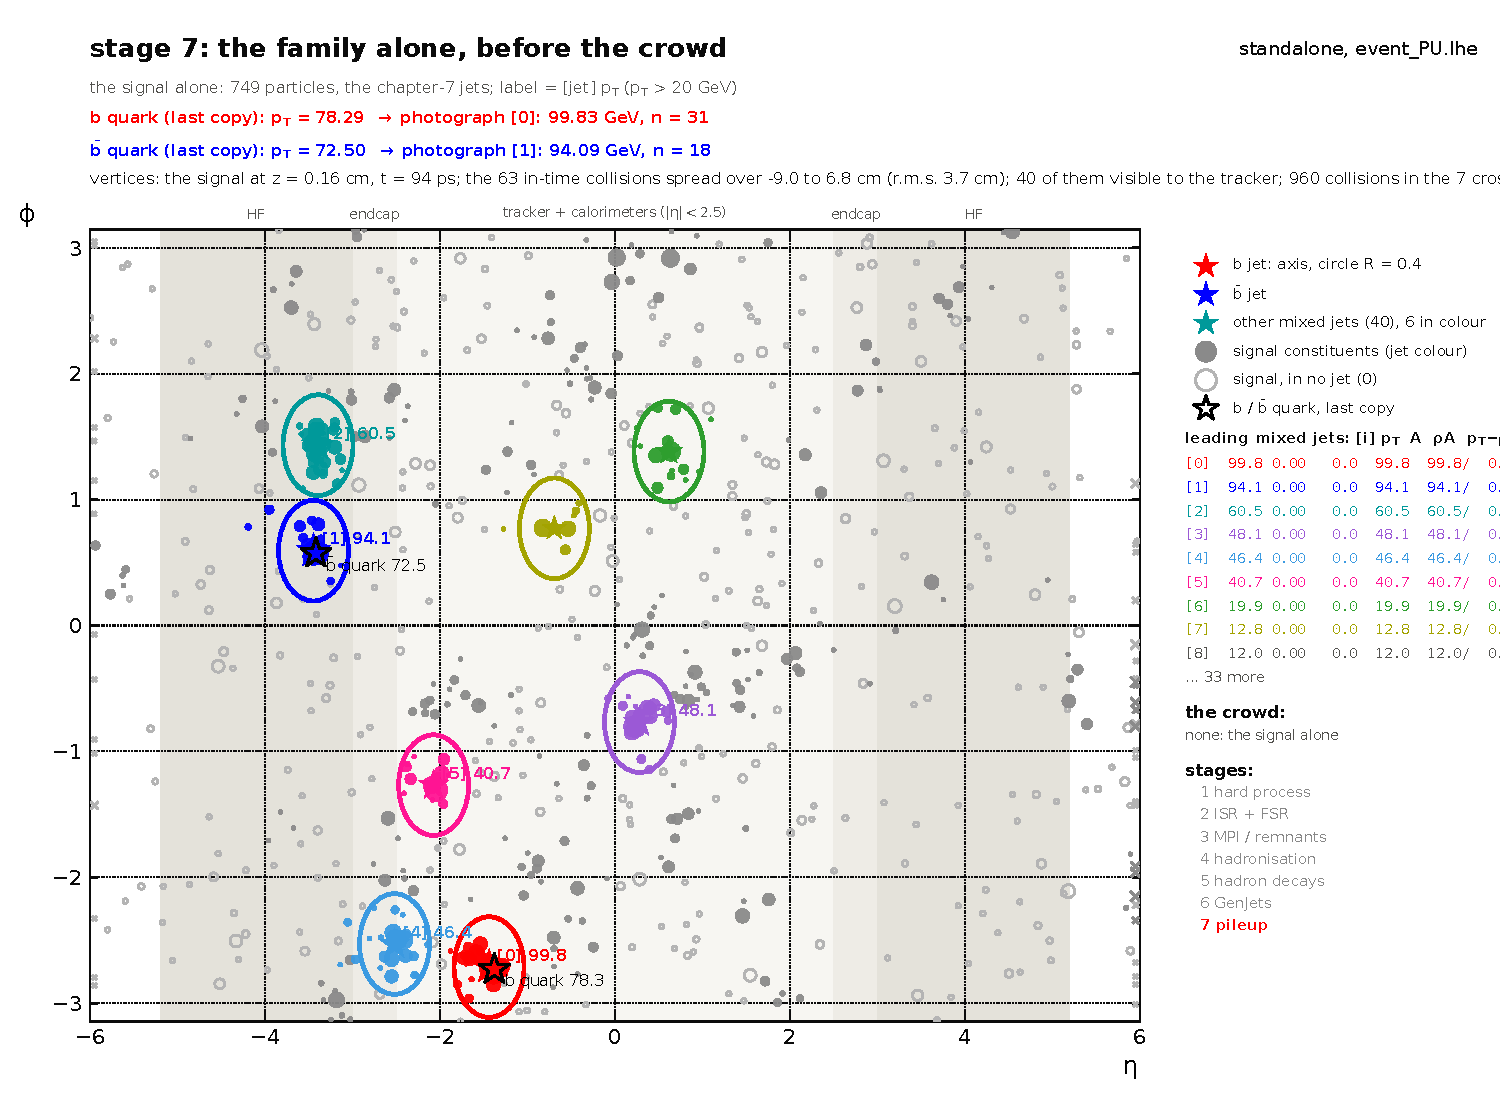
\includegraphics[width=0.495\textwidth]{PU/journey_PU_signal.pdf}\hfill
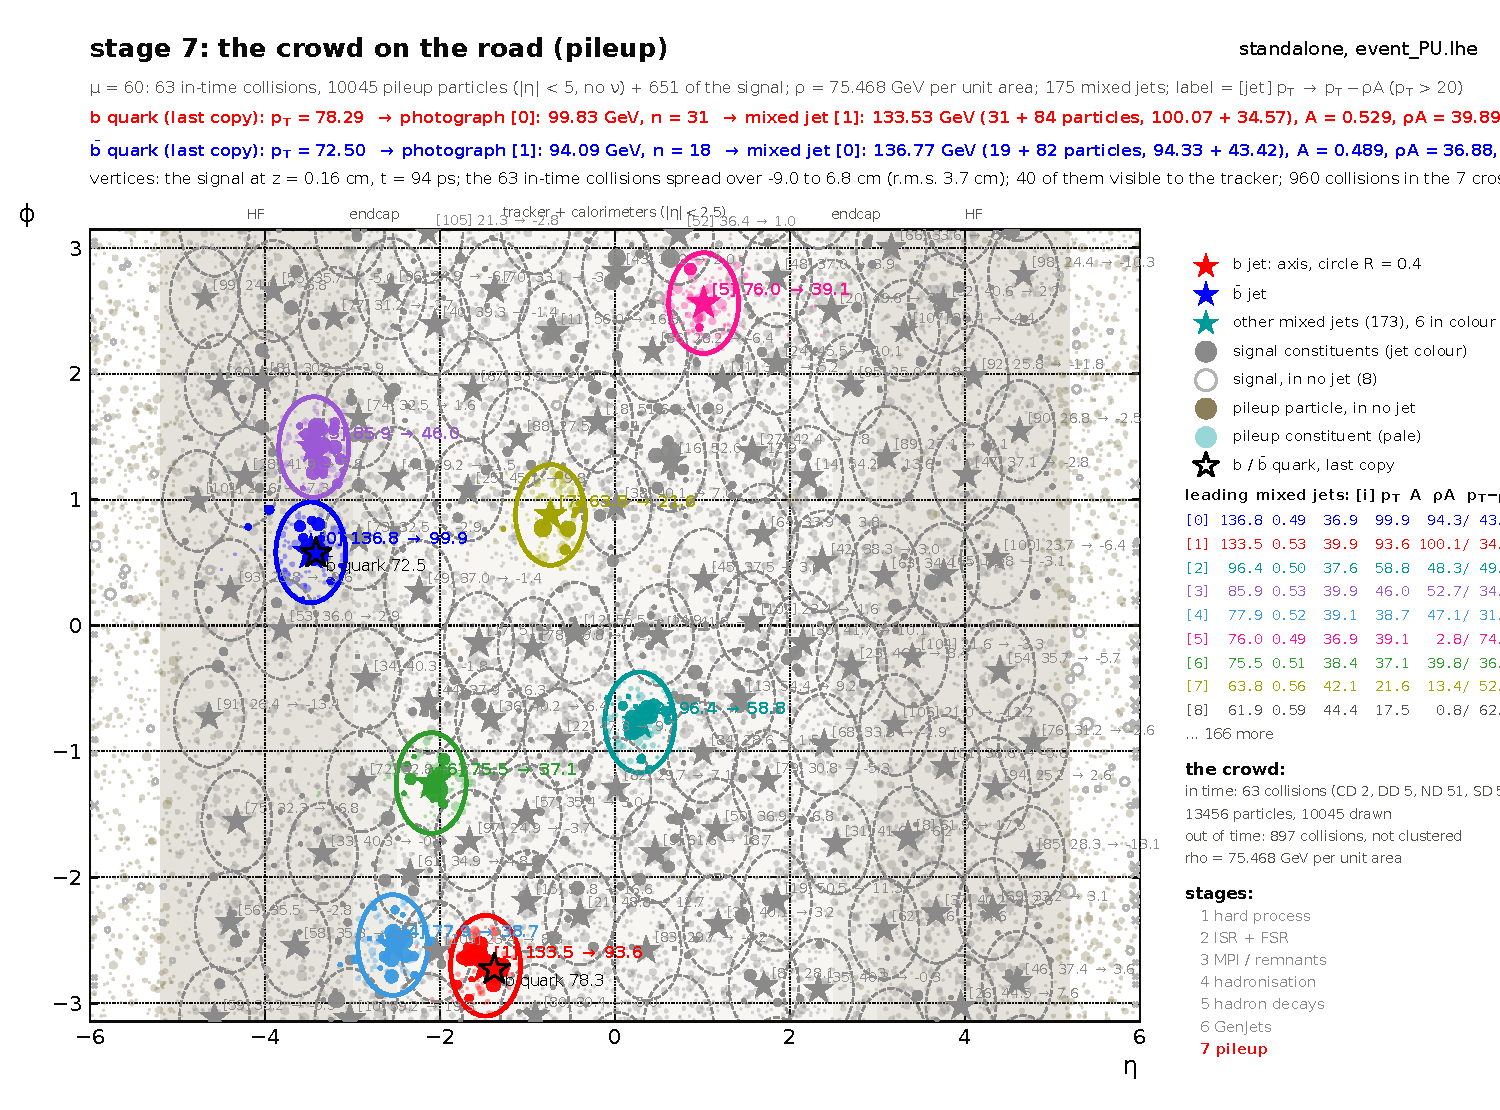
\includegraphics[width=0.495\textwidth]{PU/journey_PU.pdf}
\caption[The event before and with the crowd in the $(\eta,\phi)$
plane]{The event in the $(\eta,\phi)$ plane, in the layout of the
\CMSSW analyser pages. Left: the family alone, the photograph of
\cref{ch:family_photograph} drawn with the code of this stop. Right: the
same frame with the $63$ in-time collisions of our crossing, the crowd
in khaki, the signal particles coloured by the mixed jet that holds them,
the circles of the mixed jets with their momentum before and after the
subtraction, and our jet's line in the header: $99.83\to132.75\to96.66$.
Drawn by \file{plot_journey_PU.py} from \file{event_PU.lhe}.}
\label{fig:crowd_on_the_road:journey}
\end{figure}

\subsection{What this stop is, and what it is not}
\label{sec:crowd_on_the_road:caveats}

The agreement in \cref{tab:crowd_on_the_road:numbers} with \FASTJET is
exact where the input is identical, and the parts of the chapter that are
a model rather than a port carry their caveats:
\begin{itemize}
  \item \textbf{The crowd is \PYTHIA's.} The library is CP5's minimum
    bias, and the $0.95\GeV$ per unit area per collision is its number;
    a different tune moves it by ten percent, and the measured underlying
    event of \cite{CMS:2019csb} is what CP5 was tuned to. \rhoPU itself is
    measured in every event and does not care.
  \item \textbf{A generator-level crowd.} Every stable particle of every
    collision within $|\eta|<5$ counts here with its full momentum; the
    detector of \cref{ch:crossing_the_border} will lose the neutrals
    below its thresholds, the charged ones below $\pt\simeq0.3\GeV$ that
    curl in the field, and the forward ones in the cracks, so that the
    $\rhoPU$ of \cref{ch:paying_for_uninvited} is nearer $0.6\GeV$ per
    collision than $0.9$. The crowd shrinks; its structure does not.
  \item \textbf{One value of \mup, not the profile.} The record mixes at
    a fixed $\mup=60$, the \code{AVE\_60} of the companion's exercise; the
    production draws \mutrue flat between $55$ and $75$ and reweights,
    and a sample like this record cannot be reweighted at all. The
    ensemble draws the crowd at the same mean four hundred times, not over
    a year.
  \item \textbf{The out-of-time crowd is counted, not felt.} The $897$
    collisions of the other fifteen crossings are in the vertex listing
    with their offsets and nowhere else, because nothing at the generator
    level lasts $25\ns$. The calorimeters do, and \cref{ch:first_checkpoint}
    feels them.
  \item \textbf{The beam spot is a payload, not a model of the beams.}
    \Cref{eq:crowd_on_the_road:region} is what two head-on Gaussian
    bunches give, and \CMSSW's generator draws exactly that shape, but with
    the measured widths of early 2024 rather than widths computed from
    the bunches; a fill at the end of the year, with a different
    $\beta^*$ and crossing angle, had a different beam spot, and the real
    one is measured run by run.
  \item \textbf{The visible vertex is a proxy.} Four charged particles of
    $\pt>0.5\GeV$ within $|\eta|<2.5$ is a count, not a fit; the vertex
    finder of \cref{ch:first_checkpoint} needs tracks, and loses more of
    the crowd than the proxy does.
  \item \textbf{The subtraction is scalar.} $\pt-\rhoPU A$ corrects the
    transverse momentum and leaves the mass of the jet at its inflated
    value; the four-vector subtraction of \cite{Cacciari:2008gn}, with the
    area as a four-vector, repairs the mass too, and the substructure
    chapters will need it.
  \item \textbf{The ensemble draws the crowd, not the family.} The four
    hundred draws keep the photograph fixed and count the pileup inside a
    fixed circle, so that the $\pm7\GeV$ is the crowd's fluctuation
    alone; the mixed jet of the record, whose axis and area follow the
    crowd, adds a little to it.
  \item \textbf{One event is one sample.} The residual of $-3.41\GeV$ is
    this crossing's and the ensemble's is $-1.9\pm6.7$; the $63$
    collisions, the $34$ that reached our jet, the $68\GeV$ of \rhoPU
    against $59$ on average and the crowd vertex a twentieth of a
    millimetre from ours are this draw's.
\end{itemize}

\section{Further reading}
\label{sec:crowd_on_the_road:further_reading}
The jet area and the median density are \cite{Cacciari:2007fd}, with the
areas themselves, passive and active, in \cite{Cacciari:2008gn} and their
implementation in the \FASTJET manual~\cite{Cacciari:2011ma}; the
$\eta$-dependence of the density is \cite{Cacciari:2009dp}. The
inelastic cross section is measured in \cite{ATLAS:2016ygv,CMS:2018mlc}.
The simulation side is the \CMSSW premixing of \cite{Hildreth:2017caz}
and, for the experiment's own account of its crowd, the pileup
mitigation paper of CMS~\cite{CMS:2020ebo}, which measures \rhoPU and the
offset in Run-2 data. What comes next is in the particle-level methods,
\PUPPI~\cite{Bertolini:2014bba}, SoftKiller~\cite{Cacciari:2014gra},
constituent subtraction~\cite{Berta:2014eza} and jet
cleansing~\cite{Krohn:2013lba}, reviewed with a theorist's eye in
\cite{Soyez:2018opl}. The generator's side is \PYTHIA~8.3's
guide~\cite{Bierlich:2022pfr} for the soft processes and the tune
\cite{CMS:2019csb}. The accelerator of the open problems is the HL-LHC
design report~\cite{Apollinari:2017lhl}, with the crab cavities, the
levelling and the luminous region, and the detectors that will sort its
crowd are the Phase-2 tracker~\cite{CMS:2017lum}, the endcap
calorimeter~\cite{CMS:2017jpq} and the timing layer~\cite{Butler:2019rpu}.

\begin{pitfalls}
\begin{itemize}[nosep]
  \item \textbf{\mup is not the number of vertices.} $\mup=60$ is the
    mean of a Poisson draw; a given crossing has $60\pm8$ collisions, the
    tracker sees about $0.7\mup$ of them as vertices, and the
    \code{PileupSummaryInfo} holds all three numbers: the mean
    (\code{getTrueNumInteractions}), the draw
    (\code{getPU\_NumInteractions}) and, after reconstruction, $N_{\mathrm{PV}}$.
    Reweight on the mean, cut on the vertices, and never mix them.
  \item \textbf{40 MHz is not the crossing rate.} The bunch spacing is
    $25\ns$, but $2350$ of $3564$ slots collided in 2024: \cref{eq:crowd_on_the_road:mu}
    divides by $n_b f_{\mathrm{rev}}$, a third less, and $n_b$ changes
    with the filling scheme from year to year.
  \item \textbf{The library must match the signal.} The same beam spot,
    the same geometry, the same \GEANT, the same energy, and \emph{different
    seeds}: a library made with the default seeds of \code{cmsDriver.py}
    draws the same vertex sequence as the signal, and the first pileup
    event lands on the signal vertex in space and time. A library made
    with the HL-LHC beam spot under a 2024 signal would be wrong, and
    nothing in the job would notice.
  \item \textbf{The flat profile is not the data.} A sample mixed with
    \code{Run3\_Flat55To75} is meant to be reweighted to the measured
    profile of the year, on \mutrue; an analysis that forgets the weights
    compares data at $\langle\mup\rangle\simeq60$ with a simulation at
    $65$, and its jets are too wide and too many.
  \item \textbf{The median, not the mean.} A mean density over the plane
    includes the jets; the median does not. Conversely a median over too
    few patches, or over a region with more jets than empty patches, is a
    jet measurement in disguise.
  \item \textbf{\rhoPU is one number for the whole plane.} The crowd's
    plateau falls off at large $|\eta|$ and the detector's response with
    it; a jet in the endcap can be over-subtracted by a \rhoPU measured
    over $|\eta|<5$, and the offset corrections of
    \cref{ch:paying_for_uninvited} are binned in $\eta$ for that reason.
    \rhoPU also counts the signal's own underlying event, $3\GeV$ per
    unit area here, and subtracts it with the crowd.
  \item \textbf{$\pt-\rhoPU A$ can be negative.} A soft jet in a crowded
    event is subtracted to nothing or below; \FASTJET keeps the sign,
    \CMSSW floors the correction, and a threshold on the subtracted
    momentum is where the pileup jets of \cref{ch:the_police} start.
  \item \textbf{The area is not $\pi R^2$.} It is on average, for a lone
    hard jet; a neighbour within $2R$ takes a bite, a soft jet is irregular,
    and a jet's area fluctuates with the ghosts by a percent or two.
    Always use the active area the clustering measured.
  \item \textbf{Early and late are not in-time.} An out-of-time collision
    sits on the same beam spot $25\ns$ away; the tracker cannot tell,
    the calorimeter pulse integrates it, and a track and a cluster that
    disagree may be a crossing apart. The production window reaches
    twelve crossings back for that reason.
\end{itemize}
\end{pitfalls}

\begin{exercises}
\item Run the standalone script with \code{--mu 40} and with
  \code{--mu 75}, the edges of the Run-3 years, and compare \rhoPU, the
  pileup inside our jet and the number of pileup jets above $30\GeV$
  before the subtraction with the $\mup=60$ record. Is the pileup inside
  the circle linear in \mup? Is its fluctuation?
\item From \cref{eq:crowd_on_the_road:mu}, compute \mup for the LHC of
  2012 ($L=7.7\times10^{33}$, $n_b=1380$, $50\ns$ spacing,
  $\sigmainel=73\mbarn$ at $8\TeV$) and for 2018
  ($1.5\times10^{34}$, $2544$ bunches, $80\mbarn$), and compare with the
  $\sim21$ and $\sim37$ CMS recorded. What changes in the arithmetic when
  the spacing doubles?
\item The library has $2000$ events and a crossing uses $60$. Estimate
  the probability that a library event appears twice in the same crossing
  when read at random with replacement, and check it in the vertex listing
  of the record. Why does the production not worry about it?
\item Run the script with \code{--window 1 --sequential}, the conditions
  of the \CMSSW exercise of the companion, and compare the three draws,
  the particles per crossing and the vertex spread with the companion's
  table of mixed events. Which numbers can agree, and which cannot?
\item With \code{fill\_profile} and \code{year\_profile}, build a profile
  of a year whose fills are levelled at $62$ and compute the weights of
  \cref{eq:crowd_on_the_road:reweight} for the flat $55$--$75$ sample bin
  by bin. What fraction of the simulated events carries a weight below
  $0.1$, and what does that cost in statistical power?
\item The time spread of the beam spot is $120\ps$. Treating the
  collisions as Gaussian in time, what fraction of the crowd is within
  $\pm30\ps$ of the signal, on average? Check it against the
  \code{within 30 ps} count of the ensemble, and say what a timing layer
  with that resolution would have left of the in-time crowd.
\item Compute the grid median of the signal alone with
  \code{grid\_rho} and explain why it is $3.4\GeV$ per unit area and not
  zero. What would the $k_T$-jet median give on the signal alone, and why?
\item Draw the pileup inside the circle against the number of in-time
  collisions over the ensemble and fit a line. Compare the slope with
  $\rhoPU_1\pi R^2$ from \cref{eq:crowd_on_the_road:rho1}, and the
  scatter around the line with $\sqrt{n}$ times the per-collision
  fluctuation.
\item Replace the grid median by the mean over the cells and redo the
  subtraction of the twelve leading jets of the record. Which jets get
  worse, and by how much?
\item Change \code{GHOST\_AREA} to $0.04$ and to $0.0025$ and compare the
  areas of the leading jets and the time of the clustering. At what ghost
  area does the area of our jet stop changing within its own fluctuation?
\item A jet of $R=0.8$ has four times the area. Using the ensemble's
  numbers, estimate the pileup inside an $R=0.8$ circle around our jet and
  its fluctuation, and say why the boosted-top jets of
  \cref{ch:three_families} cannot live with $\rhoPU A$ alone.
\item Run \code{--scenario ultimate} and compare the four numbers of
  this chapter, \rhoPU, the pileup inside the circle, the residual and
  the number of pileup jets above $30\GeV$ after the subtraction, between
  $\mup=60$ and $200$. Which of them scale with \mup, which with
  $\sqrt{\mup}$, and which do neither?
\end{exercises}

\subsection*{Open problems in the context of Phase-2 LHC}
\label{sec:crowd_on_the_road:open_problems}

The crowd of this chapter is the crowd of 2024; the HL-LHC will bring
three times more of it, two hundred collisions per crossing at $14\TeV$,
and the detector CMS is building for it, with a tracker to $|\eta|=4$, a
high-granularity endcap calorimeter and a timing layer, is designed
around that number. The scripts of this stop keep that road one option
away, \code{--scenario ultimate}: the same family, $\mup=200$ in
$\bx=-3\ldots+3$, the luminous region of the crab cavities, and the
questions below can each be started with it.
\begin{enumerate}
  \item \textbf{The resolution floor.} The $\pm7\GeV$ left on a
    $100\GeV$ jet after $\rhoPU A$ at $\mup=60$ becomes $\pm14$ at
    $\mup=200$ at the generator level, and the real floor is what the jet
    energy resolution of \cite{Azzi:2019yne} assumes for every HL-LHC
    measurement with jets. With the ensemble at $\mup=60$, $140$ and
    $200$ and the per-collision density of
    \cref{eq:crowd_on_the_road:rho1}, decompose the fluctuation into its
    Poisson part, the multiplicity part and the geometric part, and ask
    which of the three the tracks of \cref{ch:the_police} and the
    $30\ps$ of the MTD~\cite{Butler:2019rpu} can remove; the open
    question is the size of the irreducible neutral part at $|\eta|>2.5$,
    where there are no tracks and the HGCAL~\cite{CMS:2017jpq} has only
    its own timing.
  \item \textbf{The density in $\eta$ and in time.} \rhoPU is one number
    here and one number in \CMSSW; the crowd's plateau is not flat and
    the detector's response to it less so, and at $\mup=200$ the
    $\eta$-dependent offset of \cref{ch:paying_for_uninvited} becomes
    the largest correction of the chain. With the library, measure
    $\rhoPU_1(\eta)$ and its fluctuation in bins of $\eta$, and ask
    whether a $\rhoPU(\eta,t)$, a density per unit area per unit time
    that the timing detectors could measure, subtracts better than
    $\rhoPU(\eta)$ for a jet whose own time is known; the question, raised
    for the MTD in \cite{Butler:2019rpu}, is open for the calorimeter jets
    that carry no track time.
  \item \textbf{Pileup jets.} At $\mup=60$ not one of the $56$ crowd jets
    above $30\GeV$ survives the subtraction; at $\mup=200$ a dozen do,
    twice as many as the family's, and every analysis with a jet veto or
    a jet count will live on the identification of
    \cref{ch:the_police}. With the jet listings of the two records,
    characterise the survivors, their number of collisions, their widths
    and their charged fractions, and ask which variable separates a crowd
    jet from a soft quark jet at the generator level; the Phase-2 question
    is whether the L1 track trigger of \cite{CMS:2020jkc} can make that
    separation at $40\,\mathrm{MHz}$.
  \item \textbf{The luminous region and the crab cavities.} The beam
    spot of 2024 is a payload fitted to data; the HL-LHC region is a
    model built from the bunches, in which the crossing angle would halve
    the overlap and the crab cavities give it back, and no data exist yet
    to fit. With \code{LuminousRegion.density} and its switches, compute
    the luminosity lost without the crab cavities and the length and the
    time spread of the region as a function of the crab angle, and ask how
    the vertex finder and the MTD should be tuned if the crabbing scheme
    changes during a fill, as the design report~\cite{Apollinari:2017lhl}
    foresees.
  \item \textbf{The library, the premixing and the profile at
    $\mup=200$.} The production premixes because the classical mixing
    cannot read $1400$ events per signal event, and the premixed sample
    loses the hit-level truth of the crowd that this chapter's pictures
    rely on; the HL-LHC profile is a spike at the levelled value with a
    tail, and a flat band like Run~3's would waste most of its events.
    With the standalone mixing, which keeps the truth at no cost, measure
    how many distinct library events a crossing needs before the reuse of
    a collision within one event becomes visible in the pileup-jet rate,
    and with \code{fill\_profile} build the mixing histogram that
    minimises the statistical cost of the reweighting for a levelled
    fill; the open question, for the Phase-2 production of
    \cite{Hildreth:2017caz}, is how small a premixed library may be
    before correlations between signal events appear in a measurement.
\end{enumerate}
The next stop takes the family and the crowd across the border, into the
detector: the magnetic field, the material, the hits, and the first
things the crowd does to them.

% ---------------------------------------------------------------------------
% Chapter 9: Crossing the Border: Detector Simulation with Geant4
% SKELETON (2026-11-15), laid out after Constitution.md rules B-E. Every
% \todo marks text, numbers or figures still to come.
% The scripts, records, logs and films of this stop will live in example/G4/,
% the technical companion is chapter/chapter_09_G4.md, and the CMSSW side
% (the GEN-SIM step of the signal event in the 2024 detector) is chapter 9
% of JitJetSW, linked from example/G4/CMSSW/README.md.
% What this stop is: the family alone, no crowd, transported by GEANT4
% through the 2024 CMS detector, the 3.8 T field and its material, down to
% SimHits. The crowd crosses the border in chapter 10 (SIM), the SimHits
% become ADC counts in chapter 11 (DIGI).
% ---------------------------------------------------------------------------
%% chapter-local shorthands
\providecommand{\placeholderfig}[1]{\fbox{\parbox[c][4cm][c]{0.9\textwidth}{\centering\todo{#1}}}}
\providecommand{\Xzero}{\ensuremath{X_0}\xspace}
\providecommand{\lambdaI}{\ensuremath{\lambda_I}\xspace}
\chapter{Crossing the Border: Detector Simulation with \GEANT}
\chaptermark{Crossing the Border}
\label{ch:crossing_the_border}

\begin{journeybox}
The family now enters a foreign country: silicon, lead tungstate, brass and
iron, under a magnetic field of $3.8$~tesla. The road bends, the luggage
gets heavier with every layer crossed, and some members of the family are
stopped at the gate for good. The border guards do not count people, they
weigh luggage, and their scales are made of material that keeps part of
what it weighs. \todo{Polish the metaphor paragraph (B1).}
\end{journeybox}

\physicsline{the 2024 CMS detector as \GEANT sees it, the material budget
in radiation and interaction lengths; charged particles in a field and in
matter: curvature, ionisation, multiple scattering, bremsstrahlung and
photon conversions; electromagnetic showers; hadronic showers, the
invisible energy and non-compensation, $e/h$; sampling calorimeters and
the SimHits of our jet. The one number to take away: \todo{the fraction
of the jet's energy that the calorimeters actually register as SimHits,
from the standalone script and \CMSSW}.}

\section{What we will see at this stop}
\label{sec:crossing_the_border:what_we_compute}

% (C1-1) motivation, connected to the previous chapter
\todo{Motivation (C1-1). Start from the end of \cref{ch:crowd_on_the_road}:
the family of \cref{ch:family_photograph} is a list of particles, and the
detector is the first place where a particle is no longer a four-vector.
This stop follows the family alone, without the crowd, so that every
SimHit is ours; the crowd crosses the border in \cref{ch:crowd_at_the_border}.
Say what is lost here (neutrinos, muons that walk through, the invisible
energy of hadronic showers, the energy left in the tracker material) and
give the four numbers to take away.}

\paragraph{The film.}
\label{sec:crossing_the_border:animation}
% (C1-2) one paragraph, at most one figure of key frames
\todo{One paragraph on the ninth film of the playlist of \jitjetworld:
the scenes, where it picks up (the crowd of \cref{ch:crowd_on_the_road})
and where it ends (the crowd crossing too).}

\begin{figure}[htbp]\centering
\placeholderfig{Key frames of the film, from
\file{example/G4/Standalone/animate_standalone_G4_stills.pdf}.}
\caption[Key frames of the animated detector-simulation stage]{Key frames
of the animated detector-simulation stage. \todo{Caption.}}
\label{fig:crossing_the_border:stills}
\end{figure}

\paragraph{The picture to carry: the family in the detector.}
% (C1-3) a sketch or diagram
\todo{The picture to carry: a quarter view of the CMS detector, our jet
entering at $\eta=-1.44$, the charged members curling in the field,
photons showering in the ECAL, hadrons in the HCAL, the muon and the
neutrinos leaving. TikZ in \file{chapter/tikz/g4_*.tex}.}

\begin{figure}[htbp]\centering
\placeholderfig{TikZ: the family crossing the CMS detector
(\file{chapter/tikz/g4_border.tex}).}
\caption[The family crossing the border]{The family crossing the border.
\todo{Caption.}}
\label{fig:crossing_the_border:border_sketch}
\end{figure}

\paragraph{The number, three ways.}
\label{sec:crossing_the_border:validation}
% (C1-4) the agreement table, one or two paragraphs
\todo{One or two paragraphs on the agreement table: the standalone script
(a NumPy transport of the family through a simplified CMS geometry), the
official package (\GEANT itself, standalone, on the same particles and the
same simplified geometry), and \CMSSW (the GEN-SIM step of the signal event
in the 2024 detector, \code{CMSSW\_15\_0\_5}). How each column is produced
is in the companion,}
\begin{center}
  \companion{chapter_09_G4}
\end{center}

\begin{table}[htbp]\centering\small
\caption[The family in the detector obtained three ways]{The family in the
detector obtained three ways. \todo{Caption: what each column is.}}
\label{tab:crossing_the_border:numbers}
\begin{tabular}{lrrr}\toprule
 & standalone & \GEANT & \CMSSW 2024 \\ \midrule
material in front of the ECAL at $\eta=-1.44$ [\Xzero] & \todo{} & \todo{} & \todo{} \\
charged members reaching the ECAL / looping & \todo{} & \todo{} & \todo{} \\
photons converted in the tracker & \todo{} & \todo{} & \todo{} \\
energy deposited in ECAL / HCAL / HF [GeV] & \todo{} & \todo{} & \todo{} \\
energy escaping: neutrinos, muons, punch-through [GeV] & \todo{} & \todo{} & \todo{} \\
visible fraction of the jet energy & \todo{} & \todo{} & \todo{} \\
SimHits: tracker / ECAL / HCAL & \todo{} & \todo{} & \todo{} \\
\bottomrule
\end{tabular}
\end{table}

\section{Let us dive into the details: the theory}
\label{sec:crossing_the_border:theory}
% Every subsection: (C2-1) motivation, (C2-2) TikZ sketch, (C2-3) equation,
% (C2-4) numbers for our event from the -v log, inline, (C2-5) one plot.

\subsection{The country: the 2024 detector, its field and its material}
\label{sec:crossing_the_border:detector}
\todo{(C2-1) Why the geometry and the material budget come first.
(C2-2) TikZ: the $r$--$z$ quarter of CMS with the subdetectors.
(C2-3) The material budget $t(\eta)=\int\mathrm{d}s/\Xzero$ and the
curvature $p_T[\GeV]=0.3\,B[\mathrm{T}]\,R[\mathrm{m}]$.
(C2-4) The numbers for our jet from the \code{-v} log.
(C2-5) Plot: material budget versus $\eta$ in \Xzero and \lambdaI.}

\subsection{A charged member in matter: ionisation and multiple scattering}
\label{sec:crossing_the_border:charged}
\todo{(C2-1) What the tracker sees of a charged hadron.
(C2-2) TikZ: a track crossing silicon layers, with its scattering angle.
(C2-3) Bethe--Bloch and the Highland formula for $\theta_0$.
(C2-4) Numbers from the \code{-v} log.
(C2-5) Plot: $\mathrm{d}E/\mathrm{d}x$ and $\theta_0$ over the momenta of
the family.}

\subsection{Photons and electrons: conversions and electromagnetic showers}
\label{sec:crossing_the_border:em_shower}
\todo{(C2-1) The photons of the $\pi^0$ decays of \cref{ch:children_getting_married} carry
a fifth of the jet.
(C2-2) TikZ: a conversion in the tracker and a shower in a crystal.
(C2-3) The conversion probability $1-e^{-7t/9}$ and the longitudinal
profile $\mathrm{d}E/\mathrm{d}t=E_0\,b\,(bt)^{a-1}e^{-bt}/\Gamma(a)$, the
Moli\`ere radius.
(C2-4) Numbers from the \code{-v} log.
(C2-5) Plot: the profile and its containment in $25.8\,\Xzero$ of
lead tungstate.}

\subsection{Hadrons: hadronic showers, the invisible energy and $e/h$}
\label{sec:crossing_the_border:had_shower}
\todo{(C2-1) Two thirds of the jet are hadrons, and the calorimeter does
not see all of their energy.
(C2-2) TikZ: a hadronic shower with its electromagnetic core, nuclear
fragments and neutrons.
(C2-3) The electromagnetic fraction $f_{\mathrm{em}}=1-(E/E_0)^{k-1}$ and
the response $\pi/e=f_{\mathrm{em}}+(1-f_{\mathrm{em}})\,h/e$; the
physics list of \CMSSW.
(C2-4) Numbers from the \code{-v} log.
(C2-5) Plot: $\pi/e$ versus energy, with the hadrons of our jet on it.}

\subsection{The scales of the guards: sampling and the SimHits}
\label{sec:crossing_the_border:sampling}
\todo{(C2-1) The HCAL samples the shower in scintillator between brass
plates; what is written is a SimHit, energy and time in an active volume.
(C2-2) TikZ: a sampling calorimeter, absorber and active layers.
(C2-3) The sampling fraction and the stochastic term
$\sigma/E=a/\sqrt{E}\oplus c$.
(C2-4) Numbers from the \code{-v} log.
(C2-5) Plot: the energy of our jet in SimHits per subdetector.}

\paragraph{The recipe.}
\todo{The recipe, step by step, that the standalone script runs.}

\section{The energy ledger: our jet at this stage}
\label{sec:crossing_the_border:ledger}
% (C3-1) the ledger table, "The same event in CMSSW", one figure page
\todo{What the record \file{example/G4/event_G4.*} holds, and what the
ledger says.}

\begin{ledgerboth}{Crossing the Border}{tab:crossing_the_border:ledger}{%
\todo{What the two blocks are.}}
\ledgerblock{Standalone (seed 1)}
\ledgerrow{the photograph, \code{ak4GenJets} jet [0] (chapter 7)}{99.83}{14.83}{31}{--}
\ledgerrow{with the crowd, after $\pt-\rhoPU A$ (chapter 8)}{93.64}{--}{115}{$-39.89$}
\ledgerrow{the family's energy in SimHits}{\todo{}}{--}{\todo{}}{\todo{}}
\ledgerblock{\CMSSW (run 1, event 1)}
\ledgerrow{the photograph, \code{ak4GenJets} jet [0] (chapter 7)}{117.79}{16.72}{24}{--}
\ledgerrow{the family's energy in SimHits}{\todo{}}{--}{\todo{}}{\todo{}}
\end{ledgerboth}

\paragraph{The same event in \CMSSW.}
\label{sec:crossing_the_border:cmssw_event}
\todo{The GEN-SIM step of JitJetSW on the signal event: the
\code{g4SimHits} of our jet, read from the log of the analyser.}

\begin{figure}[p]\centering
\placeholderfig{Standalone display: \file{G4/journey_G4.pdf}.}\\[2mm]
\placeholderfig{\CMSSW display: \file{G4/CMSSW/simHitAnalyzer_09_G4.pdf}.}
% when the files exist:
% \ledgerdisplays
%   {G4/journey_G4.pdf}{Standalone: ...}{fig:crossing_the_border:journey}
%   {G4/CMSSW/simHitAnalyzer_09_G4.pdf}{\CMSSW: ...}{fig:crossing_the_border:cmssw}
\caption[The family in the detector, standalone and \CMSSW]{The family in
the detector, standalone (top) and \CMSSW (bottom). \todo{Caption.}}
\label{fig:crossing_the_border:displays}
\end{figure}

\subsection{What this stop is, and what it is not}
\label{sec:crossing_the_border:caveats}
\begin{itemize}
  \item \todo{The family alone: no crowd, which is \cref{ch:crowd_at_the_border}.}
  \item \todo{SimHits are energy, not signals: the ADC counts are
    \cref{ch:customs_form}.}
  \item \todo{The simplified geometry of the standalone script against
    the full 2024 geometry of \CMSSW.}
  \item \todo{One event is one sample.}
\end{itemize}

\section{Further reading}
\label{sec:crossing_the_border:further_reading}
The toolkit is \GEANT~\cite{GEANT4:2002zbu}; the detector is described in
\cite{CMS:2008xjf} and its Run-3 state in \cite{CMS:2024aqx}; calorimetry
is Wigmans' book~\cite{Wigmans:2000vf}, and the passage of particles
through matter the review of the Particle Data
Group~\cite{ParticleDataGroup:2024cfk}. \todo{Literature survey: the
\CMSSW simulation, its physics lists and its validation with test-beam
data.}

\begin{pitfalls}
\begin{itemize}[nosep]
  \item \todo{Pitfall 1.}
  \item \todo{Pitfall 2.}
\end{itemize}
\end{pitfalls}

\begin{exercises}
\item \todo{Exercise 1.}
\item \todo{Exercise 2.}
\end{exercises}

\subsection*{Open problems in the context of Phase-2 LHC}
\label{sec:crossing_the_border:open_problems}
\todo{Literature survey of the Phase-2 detector simulation: the
high-granularity endcap calorimeter~\cite{CMS:2017jpq}, the Phase-2
tracker~\cite{CMS:2017lum}, the timing layer~\cite{Butler:2019rpu}, and
the cost of simulating them.}
\begin{enumerate}
  \item \todo{Open problem 1.}
  \item \todo{Open problem 2.}
\end{enumerate}
The next stop lets the crowd cross the border too.

% ---------------------------------------------------------------------------
% Chapter 10: The Crossing of the Border: The Simulated Hits
% Laid out after Constitution.md rules B-E. The scripts, records, logs and
% displays of this stop are in example/SIM/, the technical companion is
% chapter/chapter_10_SIM.md, and the CMSSW side (the full Geant4 physics stage
% by stage, the library and the MixingModule at SimHit level) is chapter 10 of
% JitJetSW, linked from example/SIM/CMSSW/README.md.
% Every standalone number is read from example/SIM/Standalone/standalone_SIM.log
% (-v, seed 1), add_hits_SIM.log, validate_SIM.log and plot_theory_SIM.json; the
% tables are the macros of example/SIM/Standalone/sim_ledger.tex.
% What this stop is: the primaries of chapter 9 cross the detector. The family,
% the in-time crowd and the out-of-time crowd are simulated separately and their
% hits are added by hand. The hits become ADC counts in chapter 11.
% ---------------------------------------------------------------------------
%% chapter-local shorthands
\providecommand{\akfour}{\code{ak4GenJets}\xspace}
\providecommand{\MeV}{\ensuremath{\,\mathrm{MeV}}\xspace}
\providecommand{\keV}{\ensuremath{\,\mathrm{keV}}\xspace}
\providecommand{\cm}{\ensuremath{\,\mathrm{cm}}\xspace}
\providecommand{\um}{\ensuremath{\,\mu\mathrm{m}}\xspace}
\providecommand{\ns}{\ensuremath{\,\mathrm{ns}}\xspace}
\providecommand{\bx}{\ensuremath{\mathrm{bx}}\xspace}
\providecommand{\Xzero}{\ensuremath{X_0}\xspace}
\providecommand{\lamI}{\ensuremath{\lambda_I}\xspace}
\providecommand{\Mix}{\code{MixingModule}\xspace}
% written by example/SIM/Standalone/add_hits_SIM.py: do not edit
\newcommand{\simLedgerRows}{%
collisions & 1 & 63 & 712 & 185 & 961 \\
primaries handed to the simulation & 672 & 10\,825 & 101\,792 & 27\,102 & 140\,391 \\
tracks: primaries and stored secondaries & 2\,680 & 32\,045 & 301\,735 & 80\,262 & 416\,722 \\
tracker hits & 8\,585 & 92\,942 & 869\,415 & 235\,071 & 1\,206\,013 \\
muon-chamber hits & 0 & 64 & 452 & 46 & 562 \\
ECAL cells with energy & 7\,704 & 50\,583 & 168\,202 & 89\,402 & 184\,475 \\
ECAL energy [GeV] & 616.6 & 4\,289.6 & 39\,433.2 & 10\,631.1 & 54\,970.4 \\
HB, HE, HO cells with energy & 1\,286 & 5\,726 & 13\,426 & 8\,934 & 14\,247 \\
HB, HE, HO scintillator energy [GeV] & 2.51 & 15.32 & 142.17 & 39.22 & 199.22 \\
HF cells with light & 496 & 1\,557 & 1\,716 & 1\,654 & 1\,721 \\
HF photoelectrons & 1\,936 & 23\,269 & 210\,265 & 57\,962 & 293\,432 \\
\midrule\multicolumn{6}{@{}l}{\emph{after the addition, each cell given to the origin that deposits most in it}}\\
ECAL cells & 1\,364 & 12\,915 & 139\,355 & 30\,841 & 184\,475 \\
\quad their energy [GeV] & 428.0 & 1\,557.6 & 48\,502.7 & 4\,482.1 & 54\,970.4 \\
HB, HE, HO cells & 153 & 771 & 11\,207 & 2\,116 & 14\,247 \\
HF cells & 2 & 2 & 1\,704 & 13 & 1\,721 \\}
\newcommand{\simTrackerRows}{%
PXB & 4 layers & 847 & 0.23 & 9\,678 & 92\,135 & 24\,809 & 127\,469 & 0.66 & 8.0 \\
PXF & $2\times3$ disks & 339 & 0.13 & 4\,919 & 45\,912 & 12\,021 & 63\,191 & 0.54 & 6.4 \\
TIB & 4 layers & 1\,563 & 0.24 & 16\,633 & 166\,516 & 45\,232 & 229\,944 & 0.68 & 8.6 \\
TID & $2\times3$ disks & 680 & 0.19 & 8\,646 & 81\,943 & 22\,091 & 113\,360 & 0.60 & 7.3 \\
TOB & 6 layers & 1\,595 & 0.41 & 13\,488 & 121\,654 & 35\,654 & 172\,391 & 0.93 & 10.6 \\
TEC & $2\times9$ disks & 3\,561 & 0.20 & 39\,578 & 361\,255 & 95\,264 & 499\,658 & 0.71 & 8.3 \\
\midrule tracker &  & 8\,585 & 0.24 & 92\,942 & 869\,415 & 235\,071 & 1\,206\,013 & 0.71 & 8.5 \\}
\newcommand{\simEcalRows}{%
EB & 61\,200 & 2\,984 & 205.7 & 20\,676 & 940.9 & 7\,433.3 & 1\,978.6 & 60\,477 & 99 & 569 \\
EE & 17\,376 & 2\,937 & 410.8 & 11\,749 & 3\,347.5 & 31\,986.7 & 8\,647.8 & 17\,375 & 100 & 86 \\
ES & -- & 1\,783 & 0.1 & 18\,158 & 1.2 & 13.2 & 4.8 & 106\,623 & -- & 709 \\}
\newcommand{\simHcalRows}{%
HB & 9\,072 & 339 & 0.64 & 2\,080 & 2.01 & 15.46 & 4.71 & 7\,741 & 85 & 98 \\
HE & 6\,768 & 947 & 1.87 & 3\,645 & 13.31 & 126.64 & 34.50 & 6\,483 & 96 & 55 \\
HO & 2\,160 & 0 & 0.00 & 1 & 0.00 & 0.07 & 0.01 & 23 & 1 & 0 \\
HF & 1\,728 & 496 & 1\,936 & 1\,557 & 23\,269 & 210\,265 & 57\,962 & 1\,721 & 100 & 2 \\}
\newcommand{\simMuonRows}{%
DT & 0 & 0 & 80 & 0 & 80 \\
CSC & 0 & 54 & 330 & 42 & 426 \\
RPC & 0 & 4 & 20 & 0 & 24 \\
GEM & 0 & 6 & 22 & 4 & 32 \\
\midrule muon system & 0 & 64 & 452 & 46 & 562 \\}
\newcommand{\simStageRows}{%
transport only (chapter 9) & 672 & 0 & 0/0/0 & 3\,419 & 0 & 0.00 & 0 & 0.0 & 0.0 & 0.00 & 0.00 & 0 & 99.8 (31) & 0.0 \\
+ magnetic field & 672 & 0 & 0/0/0 & 3\,830 & 0 & 0.00 & 0 & 0.0 & 0.0 & 0.00 & 0.00 & 0 & 94.4 (31) & 0.0 \\
+ decays in flight & 607 & 124 & 124/0/0 & 5\,033 & 0 & 0.00 & 0 & 0.0 & 0.0 & 0.00 & 0.00 & 0 & 85.4 (30) & 0.0 \\
+ electromagnetic physics & 464 & 1\,164 & 125/1039/0 & 7\,012 & 955 & 1.26 & 6\,155 & 94.3 & 240.1 & 0.77 & 2.31 & 455 & 67.7 (20) & 51.5 \\
+ hadronic physics = full & 407 & 2\,008 & 289/1302/417 & 8\,585 & 0 & 2.10 & 9\,486 & 205.7 & 410.8 & 0.64 & 1.87 & 1\,936 & 44.3 (13) & 133.5 \\}
\newcommand{\simCircleRows}{%
the family & 624 & 491 & 115.1 & 51.8 & 69 & 0.216 & 14.1 & 65.9 \\
in-time crowd (bx $=0$) & 1\,281 & 450 & 24.2 & 9.9 & 64 & 0.082 & 5.6 & 15.5 \\
early crowd (bx $-12\ldots-1$) & 14\,588 & 1\,374 & 263.7 & 115.7 & 235 & 0.783 & 54.4 & 170.1 \\
late crowd (bx $+1\ldots+3$) & 3\,722 & 960 & 73.4 & 32.2 & 145 & 0.199 & 13.7 & 45.9 \\}

\chapter{The Crossing of the Border: The Simulated Hits}
\chaptermark{The Crossing of the Border}
\label{ch:crowd_at_the_border}

\begin{journeybox}
The gate is behind them, and now the country itself begins: a land with a
wind that blows every traveller with a charge off the straight road, the
light ones into circles; with thin walls of silicon that note everyone who
walks through; with a wall of crystal in which the travellers of light give
up everything they carry, and a wall of brass behind it for the heavy ones.
Some die on the way and their children walk on. Some hit a wall too early
and arrive as a spray. Nobody crosses unchanged, and everybody leaves
footprints. The family crosses first, alone, and we follow every footprint.
Then the crowd of its own hour crosses, and then the crowds of the hours
before and after, each on the same paths as if the others were not there.
Only at the end do we lay the three sheets of footprints on top of each
other, by hand, and look for the family again.
\end{journeybox}

\physicsline{the helix in the $3.8$~T field and the loopers; decays in
flight; the energy loss of Bethe and Bloch and its Landau fluctuation in a
silicon sensor; multiple scattering, bremsstrahlung and photon conversion in
the material of the tracker, measured in radiation lengths; the
electromagnetic shower in the crystals; nuclear interactions, the hadronic
shower, its electromagnetic fraction, its invisible energy and the sampling
of the HCAL; the simulated hit; the signal, the in-time and the out-of-time
pileup simulated separately and added with a shift of $25\ns$ per bunch
crossing. The one number to take away: of the $1.2$ million hits the
tracker receives, the family owns $0.7\,\%$, and in the circle of our jet the
calorimeters receive $66\GeV$ from the family and $231\GeV$ from the crowd,
of which only $15\GeV$ arrive in our own bunch crossing.}

\section{What we will see at this stop}
\label{sec:crowd_at_the_border:what_we_compute}

\Cref{ch:crossing_the_border} ended at the gate with three lists of
\GEANT primaries, each particle at its vertex with its momentum: $672$ of
the family, $10\,825$ of the $63$ collisions of our own bunch crossing and
$128\,894$ of the $897$ collisions of the fifteen crossings around it.
Nothing had moved. At this stop everything moves. \GEANT~\cite{GEANT4:2002zbu,Allison:2016lfl}
takes each primary and follows it in steps through the CMS detector: at
every step it asks which physical process happens next, creates the
secondaries of that process and follows them in turn, and whenever a step
lies inside a \emph{sensitive} volume, a silicon sensor, a crystal, a
scintillator tile, the detector records it. Such a record is a
\emph{simulated hit}, a SimHit: for the tracker and the muon chambers a
point with a time and an energy loss, for a calorimeter the energy left in
one cell. The SimHits are what the detector \emph{received}. What its
electronics make of them is \cref{ch:customs_form}.

The standalone script of this stop, \file{standalone_SIM.py}, is not a port
of \GEANT: that toolkit and the CMS geometry it runs in are a million lines
and two million volumes. It is a simulation in the same spirit, small
enough to read: a detector written on one page with the layers, cells and
material of CMS, and for every step the formula of the textbook. Four
ingredients are switched on one after the other, as the \CMSSW companion of
this stop does with \GEANT itself: the magnetic field, the decays in flight,
the electromagnetic physics and the hadronic physics. Where \GEANT follows
the thousands of particles of a shower, the script places the energy of the
shower in the cells with a parametrisation, the idea of
\textsc{Gflash}~\cite{Grindhammer:1989zg,Grindhammer:1993kw} and of the fast
simulation of CMS~\cite{Abdullin:2011zz}.

The second half of the stop is about the crowd. The detector cannot tell
whose particle crossed it, so the crowd must be simulated too, every
collision of it. We do it the way the production does, and make the three
steps visible: the family, the in-time crowd and the out-of-time crowd are
simulated \emph{separately}, each collision as if it were alone, and their
hits are then \emph{added by hand} by a second script,
\file{add_hits_SIM.py}: times shifted by $25\ns$ per bunch crossing,
energies summed cell by cell. This is the last stop at which one can still
say which hit belongs to whom.

\paragraph{The film.}
\label{sec:crowd_at_the_border:animation}
The tenth film of the playlist of \jitjetworld shows the hits in the order
in which the detector receives them, in the longitudinal view of
\cref{fig:crowd_at_the_border:stills}: the family alone, the crowd of our
crossing alone, the fifteen other crossings each on its own clock, and then
one clock for all, on which the family is one flash among sixteen.

\begin{figure}[htbp]\centering
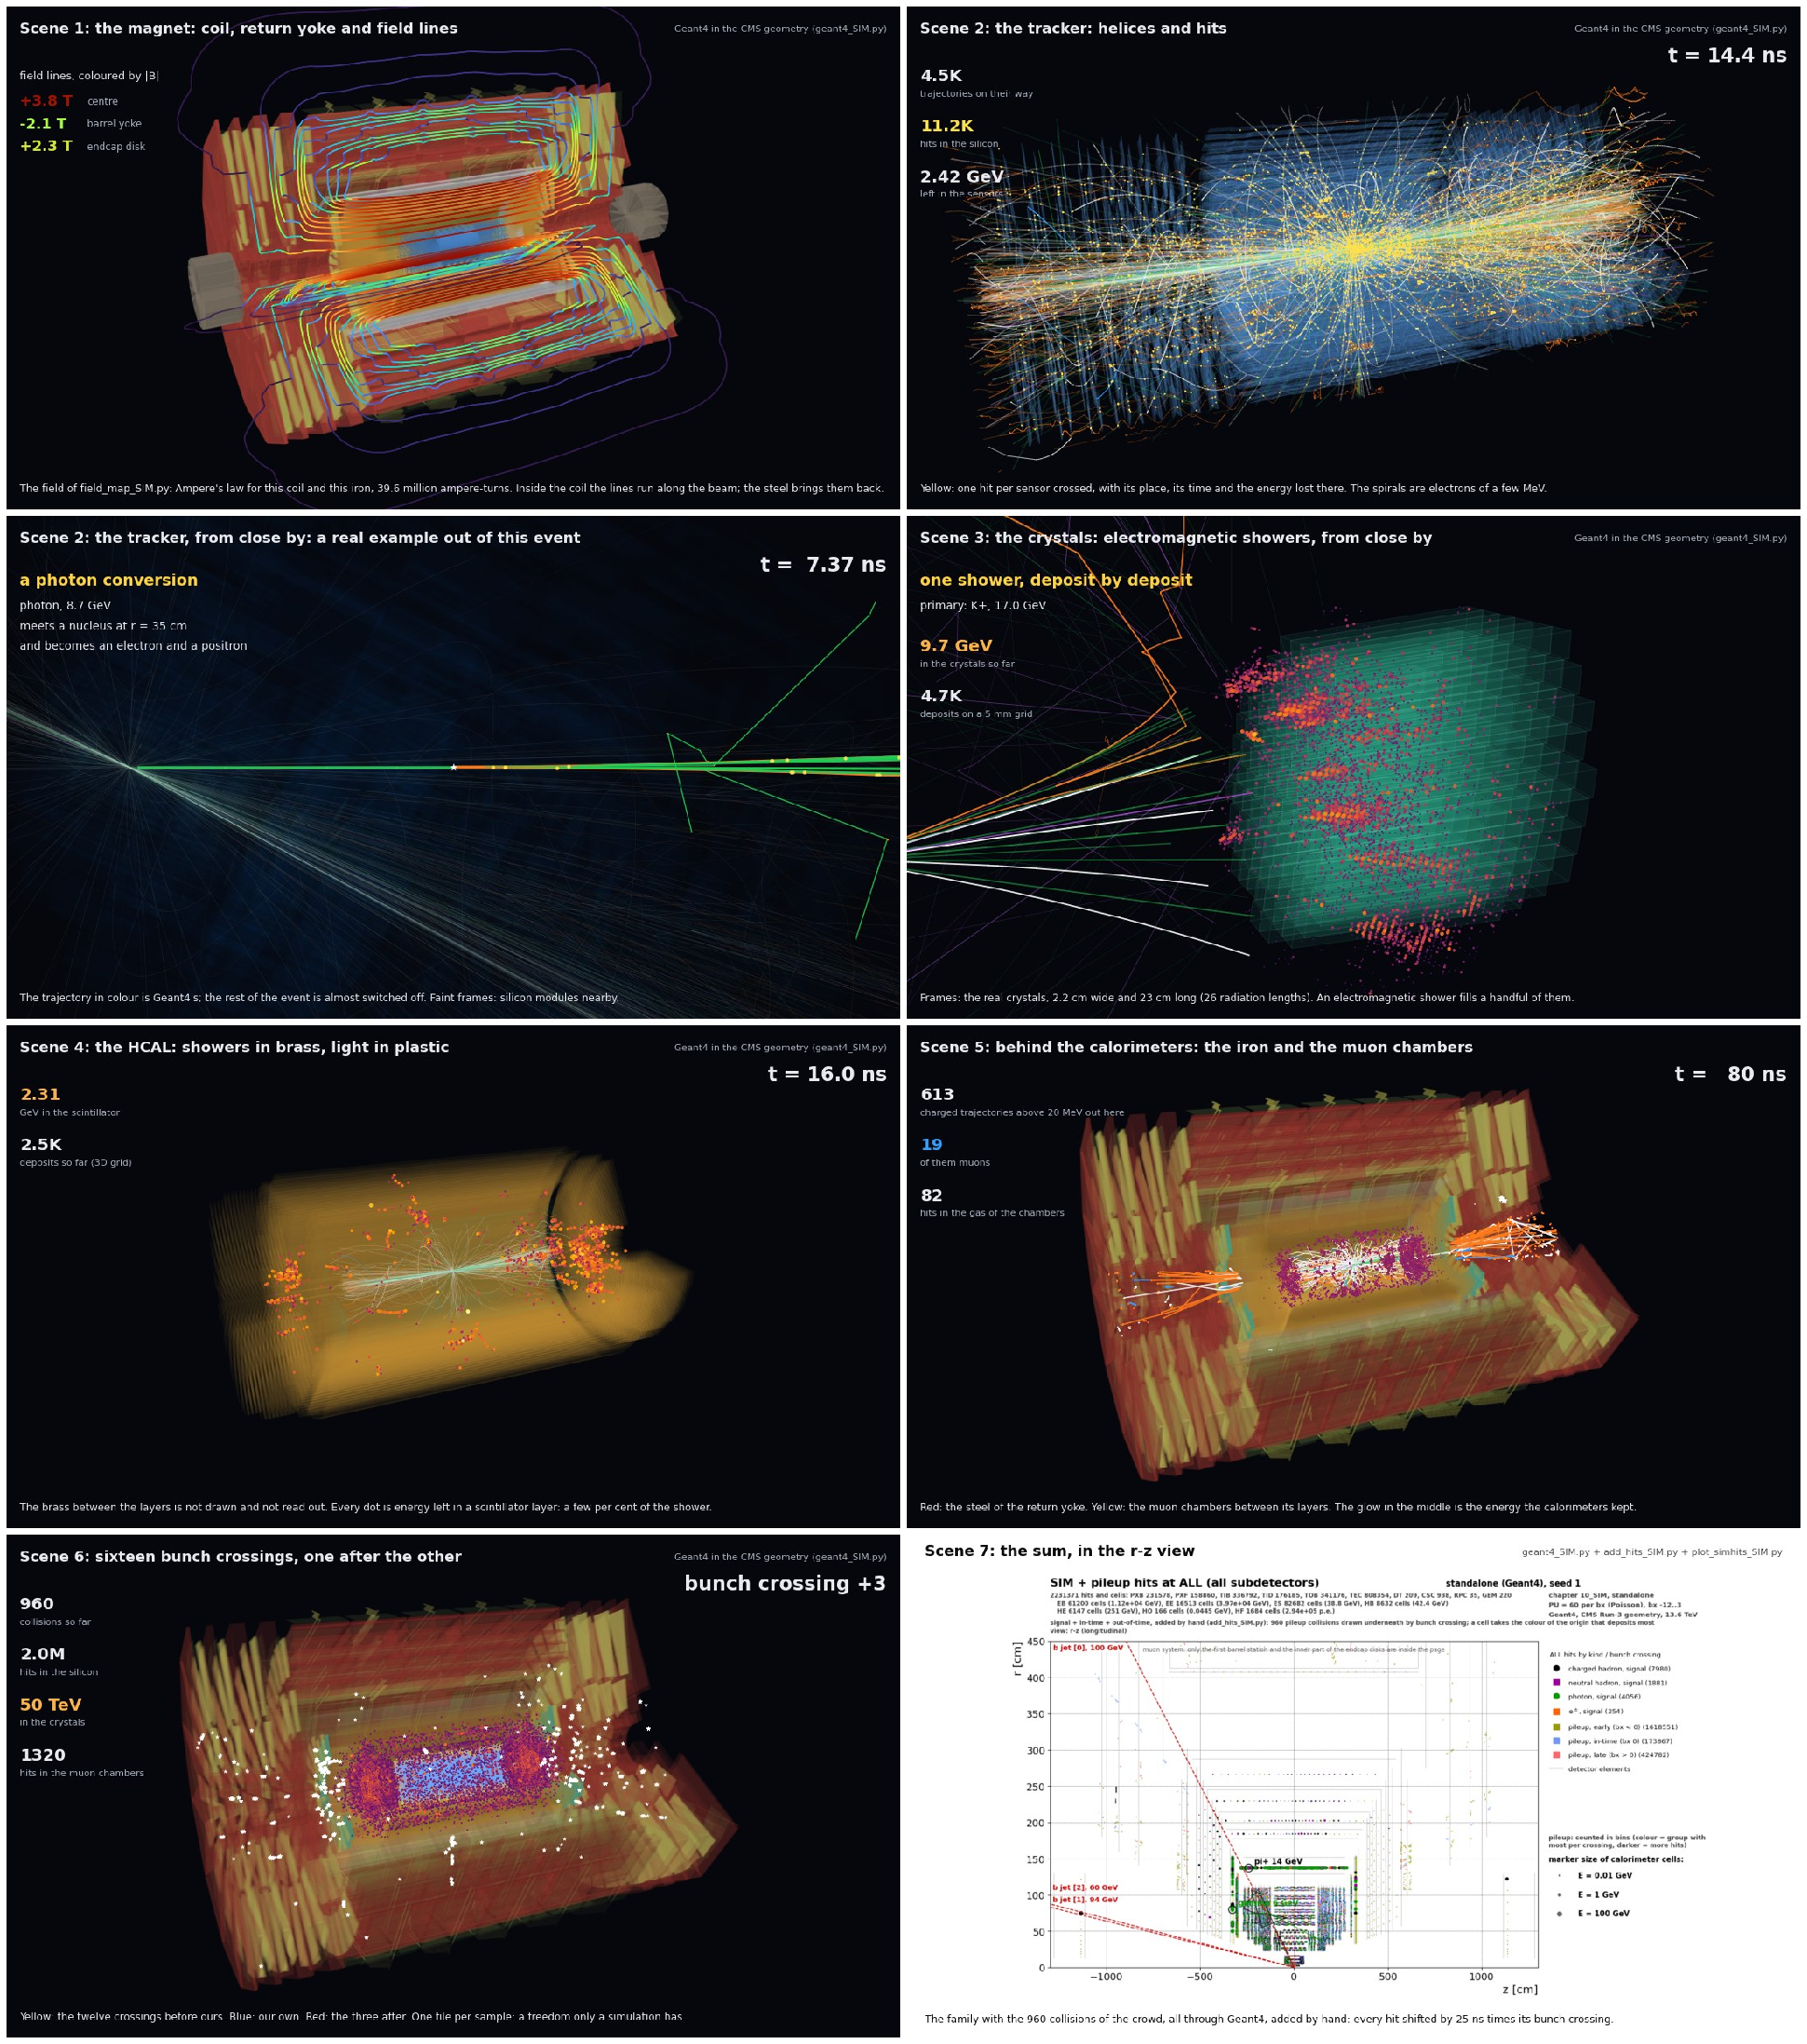
\includegraphics[width=\textwidth]{SIM/Standalone/animate_standalone_SIM_stills.pdf}
\caption[Key frames of the animated crossing]{Key frames of the animated
crossing (\file{animate_standalone_SIM.py}), $r$--$z$ view; dots are tracker
and muon hits, discs calorimeter cells. Top: the family $12\ns$ after the
collision (black), and the $63$ collisions of the same crossing (blue), each
sample simulated on its own. Bottom: the $897$ out-of-time collisions (olive
early, red late) on the clocks of their own crossings, and the sum on one
clock, $12\ns$ after our collision.}
\label{fig:crowd_at_the_border:stills}
\end{figure}

\paragraph{The picture to carry: one country, three crossings.}
\Cref{fig:crowd_at_the_border:chain} is the stop on one page. The same
detector and the same physics for everyone; three samples that never meet
inside the simulation; one addition at the end. The picture also says why
the production works this way: the crowd does not depend on the family, so
it can be simulated once and laid over any number of signal events.

\begin{figure}[htbp]\centering
\resizebox{0.9\textwidth}{!}{% chapter 10: the picture to carry. Three samples through the same detector, separately; their hits added by hand.
\begin{tikzpicture}[x=1cm,y=1cm,font=\footnotesize,>={Stealth[length=2mm]},
  box/.style={draw,rounded corners=2pt,minimum height=11mm,text width=2.55cm,align=center,inner sep=2pt},
  phys/.style={box,fill=black!6,text width=2.1cm},
  sig/.style={box,fill=red!12},it/.style={box,fill=blue!12},oot/.style={box,fill=olive!22},mx/.style={box,fill=orange!22}]
% the physics, switched on one after the other
\node[phys] (b) at (0,2.9)  {magnetic field\\{\scriptsize $R=p_T/0.3B$}};
\node[phys] (d) at (2.6,2.9) {decays in flight\\{\scriptsize $\beta\gamma c\tau$}};
\node[phys] (e) at (5.2,2.9) {EM physics\\{\scriptsize $X_0$}};
\node[phys] (h) at (7.8,2.9) {hadronic physics\\{\scriptsize $\lambda_I$}};
\draw[->] (b)--(d); \draw[->] (d)--(e); \draw[->] (e)--(h);
\draw[decorate,decoration={brace,amplitude=5pt,mirror}] (-1.2,2.2)--(9.0,2.2) node[midway,below=5pt]{the same detector and the same physics, in \GEANT, for every collision};
% three samples
\node[sig] (s)  at (-0.2,0.2)  {the family\\1 collision\\672 primaries};
\node[it]  (i)  at (3.9,0.2)  {in-time crowd\\63 collisions, bx $=0$\\10\,825 primaries};
\node[oot] (o)  at (8.0,0.2)  {out-of-time crowd\\897 collisions, 15 bx\\128\,894 primaries};
\node[sig] (sh) at (-0.2,-1.9) {\simChainSignal};
\node[it]  (ih) at (3.9,-1.9) {\simChainIntime};
\node[oot] (oh) at (8.0,-1.9) {\simChainOot};
\foreach \a/\b in {s/sh,i/ih,o/oh} \draw[->] (\a)--(\b) node[midway,right,font=\scriptsize]{simulated alone};
\node[mx,text width=5.2cm] (m) at (3.9,-4.0) {added by hand: $t\to t+25\,\mathrm{ns}\times\mathrm{bx}$,\\energies summed cell by cell\\\simChainSum};
\draw[->] (sh.south) |- (m.west); \draw[->] (ih)--(m); \draw[->] (oh.south) |- (m.east);
\draw[->] (m.south)--++(0,-0.55) node[below,font=\scriptsize,text=black!60]{the electronics: chapter 11};
\end{tikzpicture}
}
\caption[The stop on one page: three samples, one addition]{The stop on one
page. Top: the four ingredients of the simulation, switched on one after the
other in \cref{sec:crowd_at_the_border:theory}. Middle: the three samples and
what the tracker and the ECAL crystals receive from each. Bottom: the
addition by hand.}
\label{fig:crowd_at_the_border:chain}
\label{fig:crowd_at_the_border:windows_sketch}
\end{figure}

\paragraph{The number, three ways.}
\label{sec:crowd_at_the_border:validation}
\Cref{tab:crowd_at_the_border:numbers} compares the stop three ways. The
official package for the \emph{detector} is the CMS geometry itself: its
\textsc{TGeo} dump, the file of \cref{ch:crossing_the_border}, carries every
volume with its material, and ROOT's navigator~\cite{Brun:2003TGeo} follows
straight lines through it. The one-page detector of the script agrees with
it in the material in front of the calorimeters, to $1\,\%$ on average and
$8\,\%$ point by point in pseudorapidity (the layer thicknesses were tuned to
this scan, so the agreement is a closure, not a prediction), and in the
number of sensors a charged particle crosses, which was not tuned. For the
\emph{physics} the reference is the \CMSSW companion, which runs \GEANT
with the production list \code{FTFP\_BERT\_EMM} on its own event of the
same process. The two events are different draws, so the rows are compared
per primary or per collision; they agree to the tens of per cent a
parametrised simulation can claim, with one systematic difference: \GEANT
makes about $40\,\%$ more tracker hits per primary, the soft electrons and
nuclear fragments that the script does not create
(\cref{sec:crowd_at_the_border:caveats}). How each number is produced is in
the companion,
\begin{center}
  \companion{chapter_10_SIM}
\end{center}

\begin{table}[htbp]\centering\small
\caption[The crossing obtained three ways]{The crossing obtained three ways:
the standalone script (seed~1), the CMS simulation geometry scanned with
\textsc{TGeo}, and \GEANT in \CMSSW (run~1, event~1 of JitJetSW, another
event of the same process: $571$ primaries, $995$ pileup collisions).}
\label{tab:crowd_at_the_border:numbers}
\begin{tabular}{@{}lrrr@{}}\toprule
 & standalone & \textsc{TGeo} & \CMSSW 2025 \\ \midrule
material before the calorimeters, mean $x/\Xzero$ in $|\eta|<2.5$ & $1.16$ & $1.17$ & -- \\
\quad in interaction lengths, $x/\lamI$ & $0.33$ & $0.33$ & $\approx0.3$ \\
sensors crossed per charged primary, straight lines & $11.1$ & $11.8$ & $12.5$ \\
transverse momentum to reach the barrel ECAL [GeV] & $0.735$ & -- & $0.735$ \\ \midrule
tracker hits per primary, family, full physics & $12.8$ & -- & $18.0$ \\
energy loss per tracker hit [MeV] & $0.245$ & -- & $0.23$ \\
decays in flight per primary & $0.13$ & -- & $0.07$ \\
photons above $1\GeV$ that convert in the tracker & $40$ of $61$ & -- & $15$ of $29$ \\
charged hadrons that interact in the tracker & $34\,\%$ & -- & $26\,\%$ \\
HF photoelectrons, family & $1936$ & -- & $1849$ \\ \midrule
tracker hits per pileup collision & $1247$ & -- & $2107$ \\
ECAL energy per in-time collision [GeV] & $68$ & -- & $54$ \\
family's share of all tracker hits & $0.71\,\%$ & -- & $0.49\,\%$ \\
ECAL cells still dominated by the family & $1364$ of $7704$ & -- & $699$ of $12\,804$ \\
\bottomrule
\end{tabular}
\end{table}

\section{Let us dive into the details: the theory}
\label{sec:crowd_at_the_border:theory}

\subsection{The wind: the magnetic field}
\label{sec:crowd_at_the_border:field}
Why does a detector need a field? Because a tracker measures positions,
and only a curved path turns positions into a momentum. The solenoid of CMS
fills the tracker and the calorimeters with $3.8$~T along the beam. A
particle of charge $\pm1$ keeps its momentum along the field and turns in
the transverse plane on a circle of radius
\begin{equation}
  R\,[\mathrm{m}] = \frac{\pt\,[\mathrm{GeV}]}{0.3\,B\,[\mathrm{T}]}
  \quad\Rightarrow\quad R = 0.88~\mathrm{m}\times\pt\,[\mathrm{GeV}]\ \text{at}\ 3.8~\mathrm{T},
  \label{eq:crowd_at_the_border:radius}
\end{equation}
a helix in space (\cref{fig:crowd_at_the_border:helix_sketch}). A track from
the beam line gets no further from it than the diameter, so it reaches a
radius $r$ only if
\begin{equation}
  \pt > 0.3\,B\,r/2 ,
  \label{eq:crowd_at_the_border:looper}
\end{equation}
which is $0.735\GeV$ for the front face of the barrel ECAL at
$r=1.29$~m. Below it the particle is a \emph{looper}: it circles around the
beam, drifts along it and leaves the tracker through an end. A stiff track
is only deflected: its azimuth has turned by $\sin\Delta\phi=r/2R$ at radius
$r$, and over a chord $L$ it departs from the straight line by the sagitta
$s=L^2/8R$, the quantity the tracker measures.

\begin{figure}[htbp]\centering
\resizebox{0.88\textwidth}{!}{% chapter 10: the helix in the transverse plane, the sagitta and the looper.
\begin{tikzpicture}[x=1cm,y=1cm,font=\footnotesize,>={Stealth[length=2mm]}]
% (a) the circle and the sagitta
\begin{scope}
\node[font=\small\bfseries] at (2.2,4.15) {(a) a stiff track};
\draw[black!35] (0,0) circle (0.25); \draw[black!35] (0,0) ++(-10:3.3) arc (-10:75:3.3) node[above,black!60]{calorimeter, $r$};
\fill (0,0) circle (1.4pt) node[below left]{beam};
% circle of radius 6 through the origin, centre at (0,-6) rotated
\draw[red!80!black,thick] (0,0) arc (120:86.5:6.2);
\draw[dashed] (0,0)--(3.19,0.93) node[pos=0.62,below,sloped]{chord $L$};
\draw[<->] (1.6,0.47)--(1.47,0.92);
\draw[black!50,line width=0.3pt] (1.5,0.72)--(0.95,1.5) node[above,black]{sagitta $s=L^2/8R$};
\draw[->,black!60] (0,0)--(0.78,0.45) node[above left=-2pt,black!60]{$\vec p_T$};
\node[align=left] at (2.3,-1.25) {$R\,[\mathrm{m}]=\dfrac{p_T\,[\mathrm{GeV}]}{0.3\,B\,[\mathrm{T}]}$\\[2pt]$\sin\Delta\phi=r/2R$};
\node at (1.0,2.55) {$\odot\ \vec B$, 3.8 T};
\end{scope}
% (b) the looper
\begin{scope}[xshift=7.3cm]
\node[font=\small\bfseries] at (1.4,4.15) {(b) a looper};
\foreach \r in {0.5,1.0,1.5,2.0} \draw[black!25] (0,0) circle (\r);
\draw[black!35] (0,0) circle (3.0); \node[black!60] at (2.5,2.3) {$r$};
\fill (0,0) circle (1.4pt);
\draw[blue!70!black,thick] (0,-1.1) circle (1.1);
\draw[<->] (0,0)--(0,-2.2); \node at (0,-2.5) {$2R<r$};
\node[align=left] at (4.6,0.8) {never reaches $r$ if\\[2pt]$p_T<0.3\,B\,r/2$\\[2pt]$=0.735$~GeV\\for $r=1.29$~m};
\node[align=left] at (4.6,-1.4) {it crosses the\\same layers\\on every turn};
\end{scope}
\end{tikzpicture}
}
\caption[The helix in the transverse plane]{The helix in the transverse
plane. (a) A stiff track: radius, sagitta and the turn of the azimuth. (b) A
looper never reaches the calorimeter and crosses the same layers on every
turn.}
\label{fig:crowd_at_the_border:helix_sketch}
\end{figure}

For our event the log says: $307$ of the $672$ primaries are charged, $175$
of them inside the tracker, $|\eta|<2.5$, with a median \pt of $0.55\GeV$,
and $113$ of those are below $0.735\GeV$. Two thirds of the charged
particles a tracker sees can never reach the barrel calorimeter
(\cref{fig:crowd_at_the_border:field}). Switching the field on raises the
sensor crossings of the family from $3419$ on straight lines to $3830$ on
helices: the loopers cross the same layers again. The leading charged member
of our jet, a $\pi^+$ of $\pt=14.27\GeV$, has $R=12.5$~m; over $1.1$~m its
sagitta is $1.2\cm$ and its azimuth turns by $0.044$~rad. The jet as a
whole arrives at the calorimeters with $94.4$ instead of $99.8\GeV$ of
vector \pt: thirty-one tracks that no longer point where they were aimed.

\begin{figure}[htbp]\centering
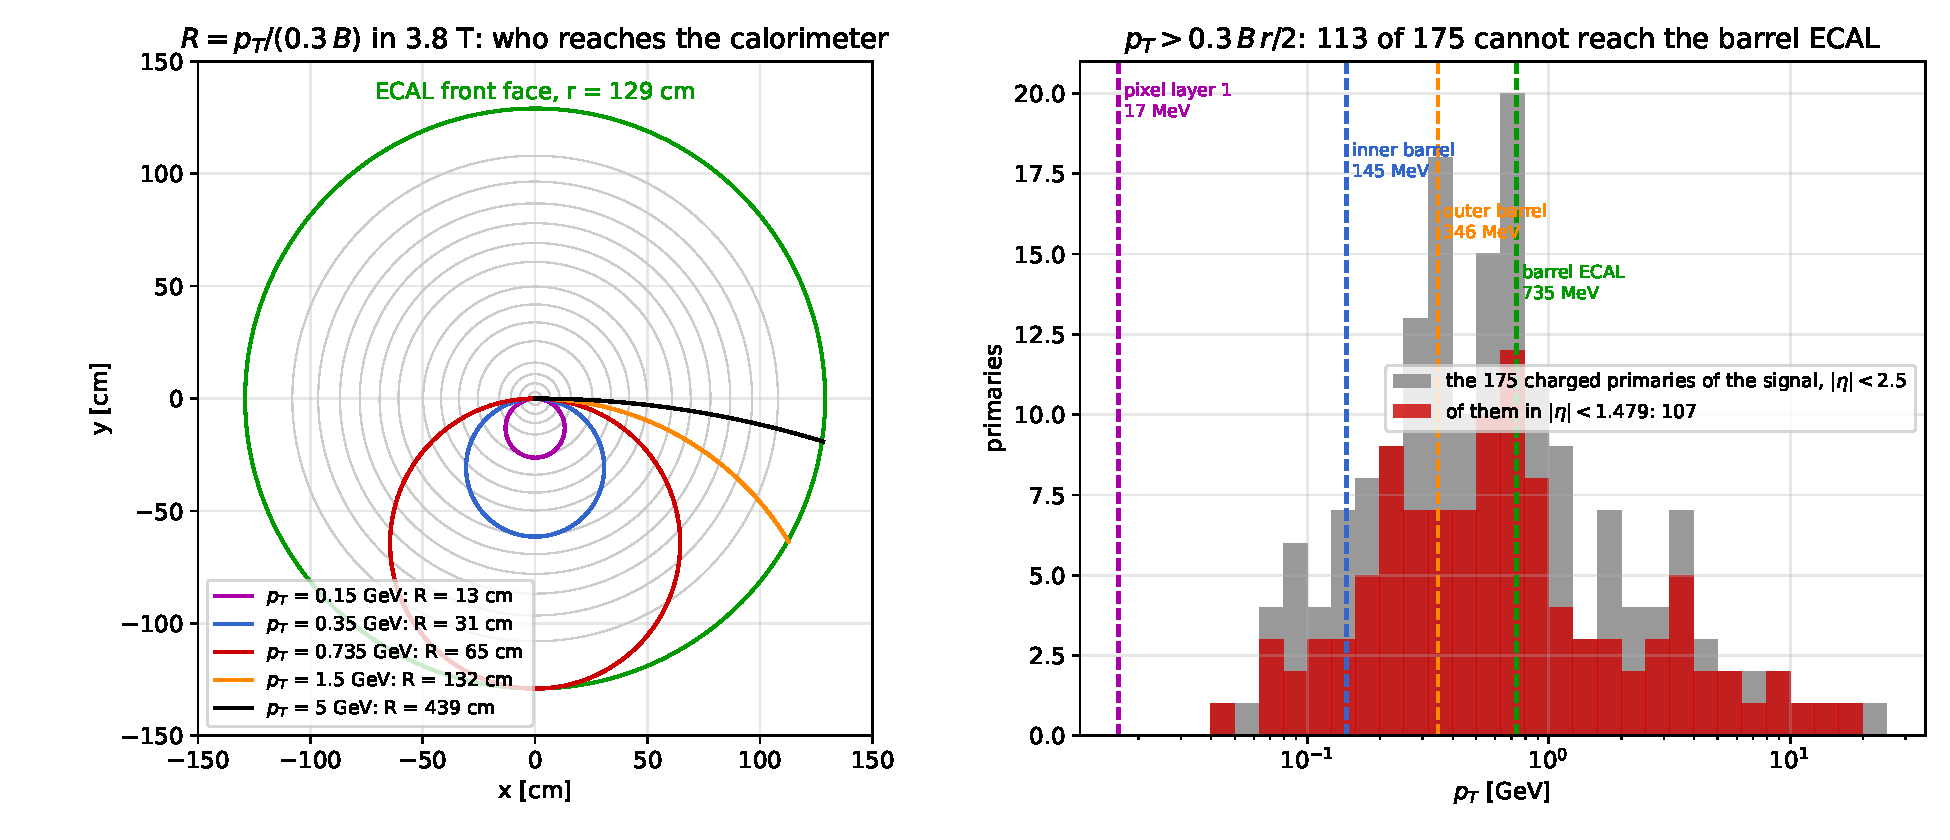
\includegraphics[page=1,width=\textwidth]{SIM/Standalone/theory_SIM.pdf}
\caption[The helix: who reaches the calorimeter]{\Cref{eq:crowd_at_the_border:radius,eq:crowd_at_the_border:looper}
for our event. Left: circles of positive particles from the beam line in
$3.8$~T, over the layers of the tracker; the red one, $0.735\GeV$, just
touches the ECAL. Right: the \pt of the charged primaries of the family and
the thresholds to reach the first pixel layer, the inner and the outer
barrel and the ECAL.}
\label{fig:crowd_at_the_border:field}
\end{figure}

\subsection{Dying on the way: decays in flight}
\label{sec:crowd_at_the_border:decays}
The generator decayed every hadron with $c\tau<10$~mm
(\cref{ch:crossing_the_border}); the long-lived ones were handed over
alive, and some of them die inside the detector. A particle of mass $m$ and
momentum $p$ flies on average $\beta\gamma c\tau=(p/m)\,c\tau$, and the
probability that it decays within a path $L$ is
\begin{equation}
  P(L) = 1-\exp\!\Big(-\frac{L\,m}{p\,c\tau}\Big).
  \label{eq:crowd_at_the_border:decay}
\end{equation}
The proper decay lengths make two classes
(\cref{fig:crowd_at_the_border:decay_sketch}): the $K^0_S$ ($d\bar s$ and
$s\bar d$, $c\tau=2.7\cm$) and the $\Lambda$ ($uds$, $7.9\cm$) decay inside
the tracker at a few \GeV, a displaced vertex of two tracks; the $\pi^\pm$
($7.8$~m) and $K^\pm$ ($3.7$~m) mostly reach the calorimeter, and when they
do decay they leave a muon and a neutrino that nobody sees.

\begin{figure}[htbp]\centering
\resizebox{0.92\textwidth}{!}{% chapter 10: who decays where. Mean flight beta gamma c tau on a scale of the detector.
\begin{tikzpicture}[x=0.085cm,y=1cm,font=\footnotesize,>={Stealth[length=2mm]}]
% the detector along a radius, in cm (0..160)
\fill[black!8] (2.25,-0.25) rectangle (16,2.95); \node[rotate=90,black!60] at (9,1.35) {pixel};
\fill[black!14] (22,-0.25) rectangle (110,2.95); \node[black!60] at (66,2.75) {strip tracker};
\fill[green!18] (129,-0.25) rectangle (152,2.95); \node[rotate=90,green!40!black] at (140.5,1.35) {ECAL crystals};
\draw[->] (0,-0.25)--(165,-0.25) node[right]{$r$ [cm]};
\foreach \x in {0,25,50,75,100,125,150} \draw (\x,-0.25)--(\x,-0.35) node[below]{\x};
% mean flights at p = 5 GeV
\draw[->,very thick,red!80!black] (0,2.3)--(27,2.3) node[right]{$K^0_S$, 5 GeV: $\beta\gamma c\tau=27$ cm $\to\pi^+\pi^-$ (a displaced vertex)};
\draw[->,very thick,violet] (0,1.6)--(35,1.6) node[right]{$\Lambda$, 5 GeV: 35 cm $\to p\,\pi^-$};
\draw[->,very thick,blue!70!black] (0,0.9)--(160,0.9); \node[blue!70!black,fill=white,inner sep=1pt] at (80,0.9) {$K^\pm$, 5 GeV: 38 m: 3\,\% decay before the ECAL};
\draw[->,very thick] (0,0.2)--(160,0.2); \node[fill=white,inner sep=1pt] at (80,0.2) {$\pi^\pm$, 5 GeV: 280 m: 0.5\,\% decay, $\pi\to\mu\nu$};
\end{tikzpicture}
}
\caption[Who decays where]{Who decays where: the mean flight
$\beta\gamma c\tau$ at $p=5\GeV$ on the radial scale of the detector.}
\label{fig:crowd_at_the_border:decay_sketch}
\end{figure}

The script draws the flight path of every such particle when it is born, as
$\beta\gamma c\tau\,(-\ln u)$ with $u$ uniform, and lets it decay there if
nothing else happens first, with the branching ratios of the table of
\cref{ch:children_producing_grandchildren}. In the full simulation of the
family $87$ particles decay in flight: $23$ $K^0_S$, $7$ $\Lambda$, $6$
$\Sigma^+$, one $K^0_L$, and $43$ pions and $7$ kaons, most of them
loopers, whose path of tens of metres makes up for their long lifetime
(\cref{fig:crowd_at_the_border:decay}). $48$ neutrinos leave unseen. The
fourth-hardest member of our jet, a $K^0_S$ of $18.7\GeV$, is one of them;
its two pions leave $102$ tracker hits that point back to no collision.

\begin{figure}[htbp]\centering
\includegraphics[page=2,width=\textwidth]{SIM/Standalone/theory_SIM.pdf}
\caption[Decays in flight]{\Cref{eq:crowd_at_the_border:decay}. Left: the
probability to decay within $1.23$~m of straight flight. Right: the $87$
decays in flight of the family in the $r$--$z$ plane of the tracker, the
$K^0_S$ and $\Lambda$ close to the beam, the looping pions everywhere.}
\label{fig:crowd_at_the_border:decay}
\end{figure}

\subsection{Footprints and tolls: electromagnetic physics in the tracker}
\label{sec:crowd_at_the_border:em}
\label{sec:crowd_at_the_border:every_collision}
A tracker should see a particle without disturbing it, and cannot: to be
seen the particle must lose energy in the sensor, and the sensor needs
supports, cables and cooling. Three things happen in every layer
(\cref{fig:crowd_at_the_border:em_sketch}a). A charged particle
\emph{ionises}: its mean energy loss per unit of matter is the Bethe-Bloch
formula~\cite{ParticleDataGroup:2024cfk},
\begin{equation}
  \Big\langle-\frac{dE}{dx}\Big\rangle = K\frac{Z}{A}\frac{1}{\beta^2}
  \Big[\tfrac12\ln\frac{2m_ec^2\beta^2\gamma^2T_{\max}}{I^2}-\beta^2-\frac{\delta}{2}\Big],
  \label{eq:crowd_at_the_border:bethe}
\end{equation}
a function of $\beta\gamma=p/m$ alone, with a minimum of $1.67\MeV\,\mathrm{cm^2/g}$
in silicon at $\beta\gamma\approx3.5$; in a thin sensor the loss fluctuates
with the long tail of Landau~\cite{Landau:1944if,Bichsel:1988if}, most
probably $84\keV$ and on average $124\keV$ in $320\um$. It is
\emph{scattered} by the nuclei, by an angle of width~\cite{Highland:1975pq,Lynch:1990sq}
\begin{equation}
  \theta_0=\frac{13.6\MeV}{\beta p}\sqrt{t}\,\big(1+0.038\ln t\big),\qquad t=x/\Xzero ,
  \label{eq:crowd_at_the_border:highland}
\end{equation}
$1.9$~mrad for a pion of $1\GeV$ crossing a layer of $2.5\,\%$ of a
radiation length. And the two lightest travellers pay a toll measured in the
same unit, the radiation length \Xzero~\cite{Tsai:1973py}: an electron
radiates, keeping on average $e^{-t}$ of its energy, and a photon converts
into an $e^+e^-$ pair with the probability
\begin{equation}
  P_{\mathrm{conv}}=1-e^{-7t/9}.
  \label{eq:crowd_at_the_border:conversion}
\end{equation}

\begin{figure}[htbp]\centering
\resizebox{\textwidth}{!}{% chapter 10: electromagnetic physics. What a layer of material does, and the shower in a crystal.
\begin{tikzpicture}[x=1cm,y=1cm,font=\footnotesize,>={Stealth[length=2mm]}]
% (a) a layer of the tracker
\node[font=\small\bfseries] at (2.3,3.3) {(a) one layer of silicon and its support};
\fill[black!15] (2.0,-0.3) rectangle (2.5,2.9); \node[rotate=90] at (2.25,1.3) {$t=x/X_0$};
% charged hadron
\draw[thick] (0,2.5)--(2.25,2.5); \draw[thick,->] (2.25,2.5)--(4.6,2.75) node[right]{$\pi$: loses $dE/dx$, scattered by $\theta_0$};
\fill[red] (2.25,2.5) circle (2pt) node[above left,red!70!black]{hit};
% electron
\draw[thick,orange!90!black] (0,1.5)--(2.25,1.5); \draw[thick,orange!90!black,->] (2.25,1.5) to[bend right=12] (4.6,1.05) node[right]{$e$: bremsstrahlung};
\draw[decorate,decoration={snake,amplitude=1pt,segment length=4pt},green!50!black,->] (2.25,1.5)--(4.6,1.62) node[right]{$\gamma$};
\fill[red] (2.25,1.5) circle (2pt);
% photon
\draw[decorate,decoration={snake,amplitude=1pt,segment length=4pt},green!50!black] (0,0.4)--(2.25,0.4);
\draw[thick,orange!90!black,->] (2.25,0.4) to[bend left=10] (4.6,0.85) node[right]{$e^+$};
\draw[thick,orange!90!black,->] (2.25,0.4) to[bend right=10] (4.6,-0.05) node[right]{$e^-$\quad conversion, $P=1-e^{-7t/9}$};
% (b) the shower in a crystal
\begin{scope}[xshift=9.6cm,yshift=1.3cm]
\node[font=\small\bfseries] at (2.4,2.0) {(b) the shower in a crystal};
\draw[fill=green!10] (0,-0.55) rectangle (5.0,0.55); \draw[black!40] (0,-1.65) rectangle (5.0,-0.55); \draw[black!40] (0,0.55) rectangle (5.0,1.65);
\draw[decorate,decoration={snake,amplitude=1pt,segment length=4pt},green!50!black,->] (-1.2,0)--(0.5,0);
\foreach \a in {-22,-12,-4,4,12,22} \draw[orange!90!black] (0.5,0)--++(\a:1.5);
\foreach \a in {-30,-20,-10,0,10,20,30} \draw[orange!90!black!70] (1.9,0.0)++(0,{\a/60})--++(\a:1.1);
\draw[<->] (0,-1.9)--(5.0,-1.9) node[midway,below]{23 cm $=25.8\,X_0$};
\draw[<->] (5.25,-0.55)--(5.25,0.55) node[midway,right]{2.2 cm $=1\,R_M$};
\draw[->] (1.75,1.95)--(1.75,0.6); \node[above] at (1.75,1.95) {$t_{max}\approx\ln(E/E_c)$};
\end{scope}
\end{tikzpicture}
}
\caption[Electromagnetic physics in a layer and in a crystal]{(a) What one
layer of the tracker does to a pion, an electron and a photon. (b) The
electromagnetic shower in a crystal of the ECAL
(\cref{sec:crowd_at_the_border:shower}).}
\label{fig:crowd_at_the_border:em_sketch}
\end{figure}

How many radiation lengths? \Cref{fig:crowd_at_the_border:material} is the
answer of the CMS geometry: $0.34\,\Xzero$ at $\eta=0$, rising to $2.0$ at
$|\eta|=1.4$, where the cables and pipes of the barrel leave the tracker,
and about $1.3$ beyond; in interaction lengths, the unit of
\cref{sec:crowd_at_the_border:hadronic}, $0.13$ to $0.45$. The script
reproduces the curve with $54$ surfaces. The consequence is on the right of
the figure: more than half of the photons convert before they reach the
calorimeter.

\begin{figure}[htbp]\centering
\includegraphics[page=4,width=\textwidth]{SIM/Standalone/theory_SIM.pdf}
\caption[The material of the tracker and what it does]{Left: the material
between the beam and the calorimeters in radiation lengths and in
interaction lengths, in the CMS simulation geometry (solid, \textsc{TGeo};
band: spread over azimuth) and in the layer model of the script (dashed).
Right: \cref{eq:crowd_at_the_border:conversion} and its hadronic twin
evaluated with the CMS material (lines), and the fraction of $5\GeV$ photons
and pions lost in the script before the calorimeters (points): $57\,\%$ and
$28\,\%$ on average.}
\label{fig:crowd_at_the_border:material}
\end{figure}

With electromagnetic physics on, the family's tracker hits carry an energy
loss, $2.10\GeV$ in $8585$ hits of the full simulation, $0.245\MeV$ per hit
(median $128\keV$; \cref{fig:crowd_at_the_border:bethe}). $313$ photons
convert, half of them in the services at the ends of the barrels, and the
electrons radiate $676$ photons above $10\MeV$. Of the $61$ primary photons
above $1\GeV$ inside the tracker, $40$ convert: by
\cref{eq:crowd_at_the_border:conversion} they crossed $1.4\,\Xzero$ on
average, as most of them fly towards the endcaps. $469$ particles, soft
electrons and loopers, stop in the tracker and never reach a calorimeter.

\begin{figure}[htbp]\centering
\includegraphics[page=3,width=\textwidth]{SIM/Standalone/theory_SIM.pdf}
\caption[The energy loss in silicon]{\Cref{eq:crowd_at_the_border:bethe}.
Left: the mean energy loss in silicon against $\beta\gamma$. Right: the
energy lost in the sensor by the family's hits in three subdetectors: a
Landau peak, shifted by the thickness and by the angle of incidence, and a
tail of slow particles.}
\label{fig:crowd_at_the_border:bethe}
\end{figure}

\subsection{The wall of crystal: the electromagnetic shower}
\label{sec:crowd_at_the_border:shower}
What stops a photon of $40\GeV$ in $23\cm$? Its own multiplication. In
lead tungstate, $\Xzero=0.89\cm$, a photon converts and an electron radiates
every centimetre, so the number of particles doubles and their energy
halves until it reaches the critical energy $E_c\approx9\MeV$, where
ionisation wins (\cref{fig:crowd_at_the_border:em_sketch}b). The energy
deposited per radiation length follows a Gamma
distribution~\cite{Grindhammer:1993kw},
\begin{equation}
  \frac{1}{E}\frac{dE}{dt}=\frac{\beta\,(\beta t)^{\alpha-1}e^{-\beta t}}{\Gamma(\alpha)},
  \qquad t_{\max}=\frac{\alpha-1}{\beta}\approx\ln\frac{E}{E_c}-0.8 ,
  \label{eq:crowd_at_the_border:gamma}
\end{equation}
with a maximum that moves only logarithmically with the energy: $3.9$,
$6.2$ and $8.5\,\Xzero$ at $1$, $10$ and $100\GeV$. A crystal of $25.8\,\Xzero$
contains them all. Across, the scale is the Moli\`ere radius, $2.19\cm$ in
lead tungstate and the width of a barrel crystal: $90\,\%$ of the energy
falls within one. The script draws $\alpha$ and $t_{\max}$ with their
fluctuations and correlation for every shower, places up to $250$ spots of
equal energy by \cref{eq:crowd_at_the_border:gamma} and a two-component
radial profile, and adds each spot to the crystal it falls in.

\Cref{fig:crowd_at_the_border:shower} shows what the tracker in front does
to this picture. Of $400$ photons of $10\GeV$ at $\eta=0.5$, the $263$
that arrive unconverted put $71\,\%$ of their energy into one crystal and
$90\,\%$ into four. The $137$ that converted arrive as two or more particles
bent apart by the field: $44\,\%$ in the hottest crystal, $90\,\%$ in ten.
Same photon, same calorimeter. The family leaves $206\GeV$ in $2984$ barrel
crystals and $411\GeV$ in $2937$ endcap crystals.

\begin{figure}[htbp]\centering
\includegraphics[page=6,width=\textwidth]{SIM/Standalone/theory_SIM.pdf}
\caption[The electromagnetic shower]{\Cref{eq:crowd_at_the_border:gamma}.
Left: the mean longitudinal profile in lead tungstate for three energies.
Right: the share of the hottest, the $9$ and the $25$ hottest crystals for
photons of $10\GeV$, unconverted (green) and converted in the tracker
(orange); bars are the spread from photon to photon.}
\label{fig:crowd_at_the_border:shower}
\end{figure}

\subsection{The wall of brass: hadronic physics}
\label{sec:crowd_at_the_border:hadronic}
\label{sec:crowd_at_the_border:in_out_of_time}
A hadron also meets the nuclei through the strong force, and its unit of
length is the nuclear interaction length \lamI, the mean path before an
inelastic collision: $20\cm$ in lead tungstate, twenty times the radiation
length. After a thickness $x$ a fraction
\begin{equation}
  P_{\mathrm{int}}=1-e^{-x/\lamI}
  \label{eq:crowd_at_the_border:lambda}
\end{equation}
has interacted. Three consequences follow. In the tracker, $0.3\,\lamI$ on
average, a third of the hadrons break up before any calorimeter: in our
event $163$ nuclear interactions, and $32$ of the $93$ charged hadrons above
$0.5\GeV$, $34\,\%$. In the crystals, $1.13\,\lamI$ deep, two hadrons in
three start their shower already in the ECAL, and one in three crosses it
as a minimum-ionising particle leaving a quarter of a \GeV. And the shower
itself is not like a photon's
(\cref{fig:crowd_at_the_border:had_sketch})~\cite{Wigmans:2000vf,Fabjan:2003aq}.
The $\pi^0$ made in every interaction decay at once to photons, and that
part of the energy showers electromagnetically; its mean fraction grows
slowly with the energy~\cite{Gabriel:1993ai,Groom:2006am},
\begin{equation}
  f_{em}=1-\Big(\frac{E}{E_0}\Big)^{k-1},\qquad E_0\approx0.8\GeV\ (\pi),\quad k\approx0.82 ,
  \label{eq:crowd_at_the_border:fem}
\end{equation}
$0.37$ at $10\GeV$ and $0.58$ at $100\GeV$, and fluctuates from one shower
to the next. Of the rest a part is \emph{invisible}: it breaks nuclei, or
leaves as slow neutrons and neutrinos. A calorimeter therefore sees a
hadron as $f_{em}+(1-f_{em})\,h/e$ of an electron of the same energy, with
$h/e\approx0.6$ to $0.7$. Finally the HCAL is a \emph{sampling}
calorimeter: brass plates stop the shower and only the thin scintillator
tiles between them are sensitive, about $1\,\%$ of the energy. A calorimeter
hit of the HCAL is that $1\,\%$; the digitisation of
\cref{ch:customs_form} multiplies it back.

\begin{figure}[htbp]\centering
\resizebox{\textwidth}{!}{% chapter 10: the hadronic shower in ECAL + HCAL: where the energy of a pion goes.
\begin{tikzpicture}[x=1cm,y=1cm,font=\footnotesize,>={Stealth[length=2mm]}]
\fill[green!12] (0,-1.5) rectangle (1.3,1.5); \node[above,align=center] at (0.65,1.5) {crystals\\$1.1\,\lambda_I$};
\foreach \x in {2.2,2.9,3.6,4.3,5.0,5.7,6.4,7.1} {\fill[orange!35] (\x,-1.5) rectangle (\x+0.5,1.5); \fill[blue!35] (\x+0.5,-1.5) rectangle (\x+0.7,1.5);}
\node[above,align=center] at (5.0,1.5) {HCAL: brass and scintillator\\$5.6\,\lambda_I$ at $\eta=0$};
\draw[thick,->] (-1.4,0)--(0,0); \node[above] at (-0.9,0.05) {$\pi^+$};
\draw[thick,dashed] (0,0)--(2.9,0); \node[below,font=\scriptsize] at (0.65,-0.1) {ionises};
\fill (2.9,0) circle (2pt);
\foreach \a/\l in {28/1.9,14/2.8,-8/3.2,-24/2.2} \draw[thick] (2.9,0)--++(\a:\l);
\draw[decorate,decoration={snake,amplitude=1pt,segment length=4pt},green!50!black,thick] (2.9,0)--++(5:1.3) node[right,font=\scriptsize]{$\pi^0\to\gamma\gamma$};
\draw[dotted,thick] (2.9,0)--++(55:1.6) node[above,font=\scriptsize]{$n$};
\draw[dotted,thick] (2.9,0)--++(-60:1.5) node[below,font=\scriptsize]{$n$};
% the budget
\begin{scope}[xshift=9.2cm,yshift=1.1cm]
\node[anchor=west,font=\small\bfseries] at (0,0.75) {a pion of $E$};
\draw[fill=green!30] (0,0) rectangle (2.2,0.5) node[midway]{$f_{em}E$};
\draw[fill=orange!30] (2.2,0) rectangle (4.6,0.5) node[midway]{charged hadrons};
\draw[fill=black!20] (4.6,0) rectangle (6.0,0.5) node[midway]{invisible};
\node[anchor=west,align=left] at (0,-0.75) {$f_{em}=1-(E/E_0)^{k-1}$: 0.37 at 10 GeV, 0.58 at 100 GeV};
\node[anchor=west,align=left] at (0,-1.45) {invisible: nuclear binding, slow neutrons, neutrinos};
\node[anchor=west,align=left] at (0,-2.15) {seen: $f_{em}+(1-f_{em})\,h/e$, and of that only the};
\node[anchor=west,align=left] at (0,-2.65) {scintillator's share, below 1\,\% (the sampling fraction)};
\end{scope}
\end{tikzpicture}
}
\caption[The hadronic shower]{A pion in the calorimeters: it ionises until
its first inelastic interaction, and the shower is part electromagnetic,
part hadronic, part invisible.}
\label{fig:crowd_at_the_border:had_sketch}
\end{figure}

The script draws the depth of the first interaction from
\cref{eq:crowd_at_the_border:lambda}, the electromagnetic fraction from
\cref{eq:crowd_at_the_border:fem} with its fluctuation, and places the
hadronic part with the longitudinal profile of Bock et
al.~\cite{Bock:1980rs} in interaction lengths. For the family, $221$ hadrons
start their shower in the crystals and $78$ in the HCAL; $158\GeV$ are
invisible, $124\GeV$ fall into the dead material between and behind the
calorimeters, and the scintillator of the barrel and endcap HCAL holds
$2.5\GeV$. \Cref{fig:crowd_at_the_border:hadronic} sends single pions into
the barrel: crystals and scintillator together, the latter multiplied by its
sampling factor, give back $0.77$ of a pion of $2\GeV$ and $0.85$ of one of
$50\GeV$, with $41\,\%$ of it in the crystals. This is the non-linear
response the jet energy corrections of \cref{ch:fair_price} exist for, and
the test beams of CMS measured the same shape~\cite{USCMS:2009fxn}. The
forward calorimeter is a different instrument: quartz fibres in steel that
see only Cherenkov light, counted in photoelectrons; the family leaves
$1936$ of them.

\begin{figure}[htbp]\centering
\includegraphics[page=7,width=\textwidth]{SIM/Standalone/theory_SIM.pdf}
\caption[The hadronic shower: electromagnetic fraction and response]{\Cref{eq:crowd_at_the_border:fem}.
Left: the electromagnetic fraction for pions and protons, and what the HCAL
and the crystals see. Right: the response of crystals plus HCAL to single
pions in the script, the share of the crystals in it, and the fraction of
pions that cross the crystals without interacting, $e^{-1.13}=0.32$.}
\label{fig:crowd_at_the_border:hadronic}
\end{figure}

\subsection{Three crowds, one clock: the addition}
\label{sec:crowd_at_the_border:crossing_frame}
\label{sec:crowd_at_the_border:premixing}
\label{sec:crowd_at_the_border:truth}
Why simulate the crowd apart? Because nothing in the detector couples two
collisions: a hit is made by one particle in one piece of matter. The hits
of an event are therefore the plain sum of the hits of its collisions, and
the only thing the sum must respect is the clock
(\cref{fig:crowd_at_the_border:clock}). A collision of bunch crossing \bx
happens $25\ns\times\bx$ away from ours, so a hit it makes at time
$t_{\mathrm{flight}}$ after its own crossing appears at
\begin{equation}
  t=t_{\mathrm{flight}}+25\ns\times\bx,\qquad
  E_{\mathrm{cell}}=\sum_{\bx=-12}^{+3}\ \sum_{\mathrm{hits}\,\in\,\bx}E_{\mathrm{hit}} .
  \label{eq:crowd_at_the_border:sum}
\end{equation}
That is all \file{add_hits_SIM.py} does, and all the \Mix of \CMSSW does at
this level~\cite{Hildreth:2017caz}: it stamps every hit with its crossing
and its collision, and lays them in one frame.

\begin{figure}[htbp]\centering
\resizebox{0.95\textwidth}{!}{% chapter 10: sixteen bunch crossings on one clock, and one cell that adds them.
\begin{tikzpicture}[x=0.72cm,y=1cm,font=\footnotesize,>={Stealth[length=2mm]}]
\draw[->] (-13,0)--(5,0) node[right]{$t$};
\foreach \b/\n in {-12/60,-11/56,-10/68,-9/61,-8/66,-7/56,-6/55,-5/50,-4/53,-3/66,-2/61,-1/60} {
  \fill[olive!70] (\b-0.3,0) rectangle (\b+0.3,{\n/45}); \node[font=\tiny] at (\b,{\n/45+0.15}) {\n}; \node[font=\tiny,below] at (\b,0) {\b};}
\fill[blue!60] (-0.3,0) rectangle (0.3,{63/45}); \node[font=\tiny] at (0.15,{63/45+0.15}) {63};
\fill[red!80!black] (-0.3,{63/45}) rectangle (0.3,{63/45+0.25}); \node[font=\tiny,red!80!black,anchor=west] at (0.35,{63/45+0.32}) {+ the family};
\node[font=\tiny,below] at (0,0) {\textbf{0}};
\foreach \b/\n in {1/63,2/59,3/63} {\fill[red!45] (\b-0.3,0) rectangle (\b+0.3,{\n/45}); \node[font=\tiny] at (\b,{\n/45+0.15}) {\n}; \node[font=\tiny,below] at (\b,0) {+\b};}
\node[below] at (-12,-0.3) {$-300$ ns}; \node[below] at (0,-0.3) {0}; \node[below] at (3,-0.3) {$+75$ ns};
\draw[decorate,decoration={brace,amplitude=5pt}] (-12.3,2.0)--(-0.7,2.0) node[midway,above=5pt]{early: 712 collisions, simulated one by one};
\draw[decorate,decoration={brace,amplitude=5pt}] (0.7,2.0)--(3.3,2.0) node[midway,above=5pt]{late: 185};
% one cell
\node[draw,fill=green!12,minimum width=1.6cm,minimum height=1.1cm,align=center] (c) at (-4,-2.3) {one cell\\$E=\sum_{bx}\sum_{hits}E_{hit}$};
\foreach \b in {-10,-7,-3,0,2} \draw[->,black!60] (\b,-0.75) -- (c);
\node[align=left,anchor=west] at (-1.6,-2.3) {every hit keeps its time $t=t_{flight}+25\,\mathrm{ns}\times bx$\\and the collision it came from; nothing is lost in the sum};
\end{tikzpicture}
}
\caption[Sixteen crossings on one clock]{Sixteen bunch crossings on one
clock: the collisions drawn for each in \cref{ch:crowd_on_the_road}, and one
cell that adds what all of them leave in it.}
\label{fig:crowd_at_the_border:clock}
\end{figure}

The crowd is very unequal. A collision leaves $8.6$ tracker hits per
primary and $1247$ on average, but the median is $725$ and the largest
leaves $8102$; in the crystals $57\GeV$ on average. On one clock
(\cref{fig:crowd_at_the_border:time}) the sixteen crossings are sixteen
bursts of hits $25\ns$ apart, each with a tail of loopers and slow
particles that reaches into the next; the family's $8585$ hits are one line
under the burst of the $92\,942$ of its own crossing. In the circle of our
jet, $\Delta R<0.4$, the cells receive $66\GeV$ of transverse energy from
the family and $231\GeV$ from the crowd, $14.5\GeV$ per crossing and
$15.5\GeV$ from our own. Which of the fifteen other crossings a detector
still sees is decided by its electronics: the tracker listens for one
crossing, the crystals and the tiles for several. That is
\cref{ch:customs_form}; here every hit is kept, with its time.

\begin{figure}[htbp]\centering
\includegraphics[page=8,width=\textwidth]{SIM/Standalone/theory_SIM.pdf}
\caption[The three crowds in time]{\Cref{eq:crowd_at_the_border:sum}. Left:
the time of every tracker hit after the shift, by origin. Right: the
transverse energy the cells within $\Delta R<0.4$ of our jet receive from
each bunch crossing (HCAL cells multiplied by their sampling factor).}
\label{fig:crowd_at_the_border:time}
\end{figure}

\paragraph{The recipe.}
\Cref{fig:crowd_at_the_border:flow} is the loop the script runs for every
particle. (1)~Take a particle from the stack and, if it is unstable, draw
its decay path. (2)~Follow the helix, or the line, to the next surface of
the tracker. (3)~If the decay path ends first, decay and stack the
daughters. (4)~At the surface: record a hit if it is a sensor; subtract the
energy loss of \cref{eq:crowd_at_the_border:bethe}; scatter by
\cref{eq:crowd_at_the_border:highland}; let an electron radiate, a photon
convert by \cref{eq:crowd_at_the_border:conversion}, a hadron interact by
\cref{eq:crowd_at_the_border:lambda}, and stack what comes out. (5)~At the
boundary of the tracker follow the particle to the face of the ECAL or of
the HF. (6)~There a photon or electron showers by
\cref{eq:crowd_at_the_border:gamma}; a hadron ionises to its first
interaction and showers by \cref{eq:crowd_at_the_border:fem}; a muon ionises
through everything to the muon stations. (7)~Repeat for the $672$ primaries
of the family, then, with other random numbers, for each collision of the
crowd on the clock of its own crossing. (8)~Add by
\cref{eq:crowd_at_the_border:sum}.

\begin{figure}[htbp]\centering
\resizebox{\textwidth}{!}{% chapter 10: the recipe of standalone_SIM.py for one particle.
\begin{tikzpicture}[x=1cm,y=1cm,font=\footnotesize,>={Stealth[length=2mm]},
  b/.style={draw,rounded corners=2pt,fill=black!5,minimum height=9mm,text width=2.9cm,align=center,inner sep=2pt},
  d/.style={draw,diamond,aspect=2.4,fill=yellow!15,inner sep=1pt,align=center,text width=2.1cm}]
\node[b] (a) at (0,0) {take a particle from the stack; draw its decay path $\beta\gamma c\tau(-\ln u)$};
\node[b] (h) at (4.2,0) {helix (or line) to the next surface of the tracker};
\node[d] (q) at (8.5,0) {decay path reached first?};
\node[b] (dc) at (12.6,0) {decay: daughters on the stack};
\node[b] (m) at (8.5,-2.3) {at the surface: hit, $dE/dx$, scattering, bremsstrahlung, conversion, nuclear interaction};
\node[d] (e) at (4.2,-2.3) {boundary of the tracker?};
\node[b] (c) at (0,-2.3) {to the face of ECAL or HF; shower, or ionise through to the muon stations};
\node[b,fill=green!12] (o) at (0,-4.3) {cells: energy and time per primary};
\node[b,fill=red!10] (t) at (8.5,-4.3) {tracker hit: position, time, $dE$, primary};
\draw[->] (a)--(h); \draw[->] (h)--(q); \draw[->] (q)--node[above]{yes}(dc); \draw[->] (q)--node[right]{no}(m);
\draw[->] (m)--(e); \draw[->] (e)--node[above]{yes}(c); \draw[->] (e)--node[right]{no}(h);
\draw[->] (c)--(o); \draw[->] (m)--(t);
\draw[->] (dc.north) -- ++(0,0.5) -| (a.north);
\draw[->] (m.east) -- ++(1.0,0) node[right,align=left]{secondaries\\on the stack};
\end{tikzpicture}
}
\caption[The recipe of the standalone simulation]{The loop of
\file{standalone_SIM.py} for one particle.}
\label{fig:crowd_at_the_border:flow}
\end{figure}

\section{The energy ledger: our jet at this stage}
\label{sec:crowd_at_the_border:ledger}

The record \file{example/SIM/event_SIM.lhe} is the record of
\cref{ch:crossing_the_border} followed by three tables: the summary of the
hits, one row per primary of the family (what ended it as a primary, where
it left the tracker, its hits and the energy it left in each calorimeter),
and one row per collision of the crowd. The hits themselves, $1.2$ million
points and $200\,000$ cells, are in three binary files, one per sample.
\Cref{tab:crowd_at_the_border:stages} is the family alone, one ingredient
more in each row, and \cref{tab:crowd_at_the_border:hits_ledger} is the
ledger of the three samples and of their sum.

\begin{table}[htbp]\centering\scriptsize\setlength{\tabcolsep}{2.6pt}
\caption[The physics switched on stage by stage]{The physics switched on
stage by stage, for the family (\file{standalone_SIM.log}): primaries
leaving the tracker intact (of $672$), stored secondaries and their origin
(decay / electromagnetic / hadronic), tracker and muon-chamber hits, the
energy lost in the sensors [GeV], calorimeter cells, energy per subdetector
(GeV; HB, HE: in the scintillator; HF: photoelectrons), and our jet: vector
\pt [GeV] of its members still primaries at the boundary (their number) and
the energy they leave in the crystals. The $955$ muon-chamber hits of the
fourth row are hadrons crossing the calorimeters like muons, as long as
nothing makes them interact.}
\label{tab:crowd_at_the_border:stages}
\resizebox{\textwidth}{!}{%
\begin{tabular}{@{}lrrrrrrrrrrrrrr@{}}\toprule
stage & bound. & \multicolumn{2}{c}{secondaries} & \multicolumn{2}{c}{hits} & $\sum dE$ & cells & EB & EE & HB & HE & HF & jet \pt & jet \\
 & & all & dec/EM/had & tracker & muon & & & & & & & & at bound. & ECAL \\ \midrule
\simStageRows
\bottomrule
\end{tabular}}
\end{table}

\begin{table}[htbp]\centering\footnotesize\setlength{\tabcolsep}{4pt}
\caption[The ledger of the hits: three samples and their sum]{The ledger of
the hits (\file{add_hits_SIM.log}): the family, the in-time crowd and the
out-of-time crowd, split into its twelve early and three late crossings,
each simulated separately, and their sum. For cells the last column is the
number of distinct cells. Below the line every cell of the sum is given to
the origin that deposited most of its energy, as the \CMSSW companion's
ledger does.}
\label{tab:crowd_at_the_border:hits_ledger}
\begin{tabular}{@{}lrrrrr@{}}\toprule
 & the family & in time & early & late & added \\
 & & \bx $=0$ & \bx $-12\ldots-1$ & \bx $+1\ldots+3$ & \\ \midrule
\simLedgerRows
\bottomrule
\end{tabular}
\end{table}

\paragraph{Station by station.}
\label{sec:crowd_at_the_border:stations}
\Cref{tab:crowd_at_the_border:trk,tab:crowd_at_the_border:calo,tab:crowd_at_the_border:muon}
take the same sum detector by detector, and
\cref{fig:crowd_at_the_border:stations_signal,fig:crowd_at_the_border:stations_mixed}
draw it. In the \emph{tracker} the endcap disks of the strip tracker hold $41\,\%$ of the hits,
the family's and the crowd's alike, and the family is $8.5\,\%$ of the hits
of its own crossing and $0.7\,\%$ of all sixteen. In the \emph{ECAL} the
crowd reaches $99\,\%$ of the barrel crystals and every endcap crystal; the
family deposits in $7704$ cells and remains the largest depositor in $1364$
of them, which hold $428$ of its $617\GeV$: the cores of its showers
survive, their edges belong to someone else. In the \emph{HCAL} the early
crossings own four cells in five. The \emph{muon chambers} receive nothing
from this family and $562$ hits from the crowd: muons of pion and kaon
decays and of the crowd's own heavy flavour, most of them in the endcap.

\begin{table}[htbp]\centering\footnotesize\setlength{\tabcolsep}{3.5pt}
\caption[The tracker, subdetector by subdetector]{The tracker: hits by
subdetector and origin, the mean energy loss per hit of the family, and the
family's share of all hits and of the hits of its own bunch crossing.}
\label{tab:crowd_at_the_border:trk}
\begin{tabular}{@{}llrrrrrrrr@{}}\toprule
 & & \multicolumn{2}{c}{the family} & in time & early & late & added & \multicolumn{2}{c}{family's share [\%]} \\
 & & hits & MeV/hit & & & & & of all & of \bx 0 \\ \midrule
\simTrackerRows
\bottomrule
\end{tabular}
\end{table}

\begin{table}[htbp]\centering\scriptsize\setlength{\tabcolsep}{3pt}
\caption[The calorimeters, subdetector by subdetector]{The calorimeters:
cells of the detector of the script, cells with energy and the energy by
origin (GeV; HB, HE, HO: energy in the scintillator; HF: photoelectrons),
the cells hit after the addition and their share of the detector, and the
cells in which the family is still the largest depositor.}
\label{tab:crowd_at_the_border:calo}
\resizebox{\textwidth}{!}{%
\begin{tabular}{@{}lrrrrrrrrrr@{}}\toprule
 & cells in & \multicolumn{2}{c}{the family} & \multicolumn{2}{c}{in time} & early & late & \multicolumn{2}{c}{added} & family \\
 & detector & cells & energy & cells & energy & energy & energy & cells & [\%] & keeps \\ \midrule
\simEcalRows
\midrule
\simHcalRows
\bottomrule
\end{tabular}}
\end{table}

\begin{table}[htbp]\centering\footnotesize
\caption[The muon system]{The muon system: hits by origin.}
\label{tab:crowd_at_the_border:muon}
\begin{tabular}{@{}lrrrrr@{}}\toprule
 & the family & in time & early & late & added \\ \midrule
\simMuonRows
\bottomrule
\end{tabular}
\end{table}

\begin{figure}[htbp]\centering
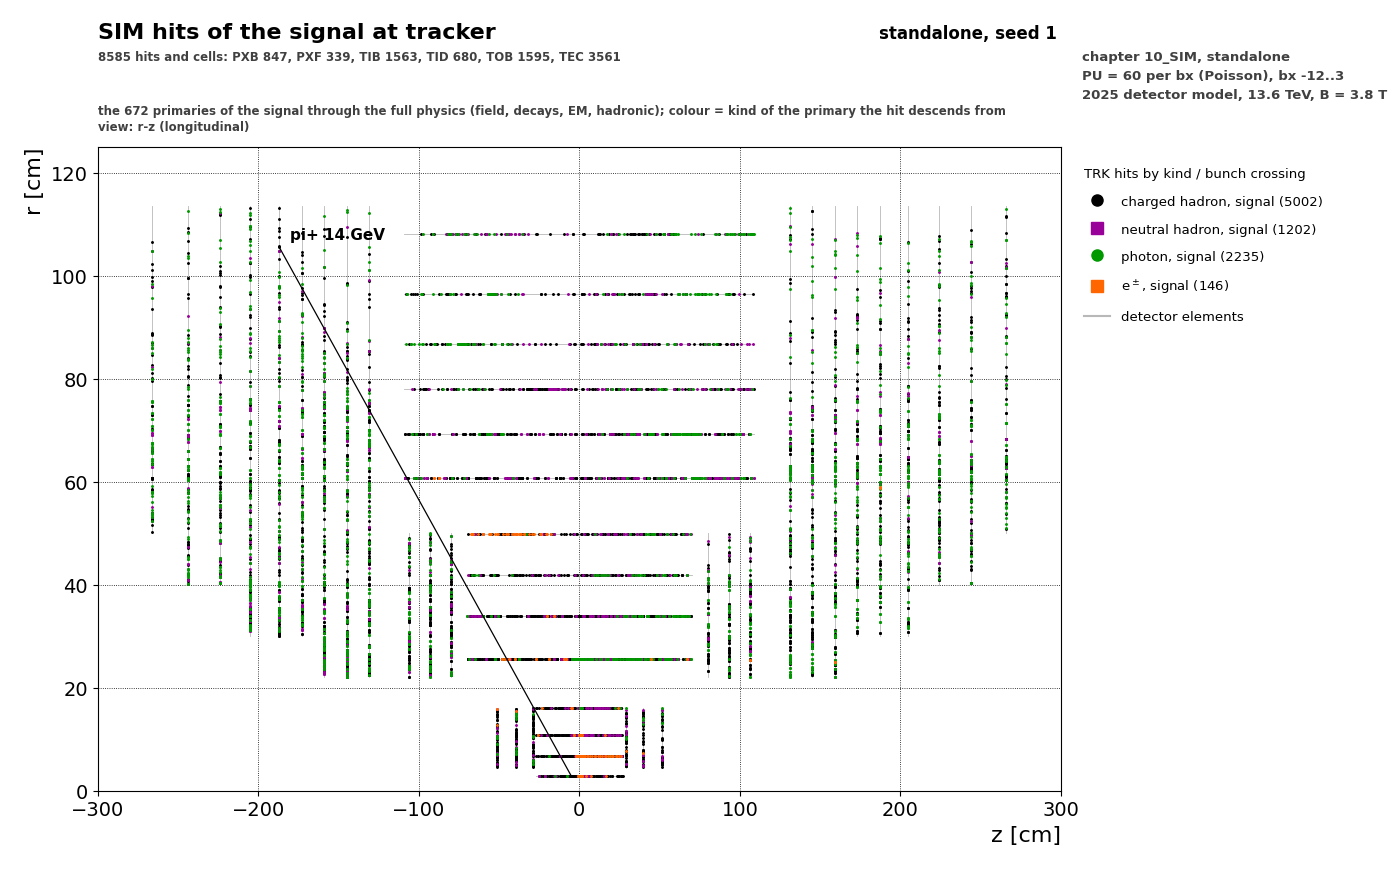
\includegraphics[width=0.495\textwidth]{SIM/Standalone/pages/simHits_signal_10_SIM_TRK_rz.png}\hfill
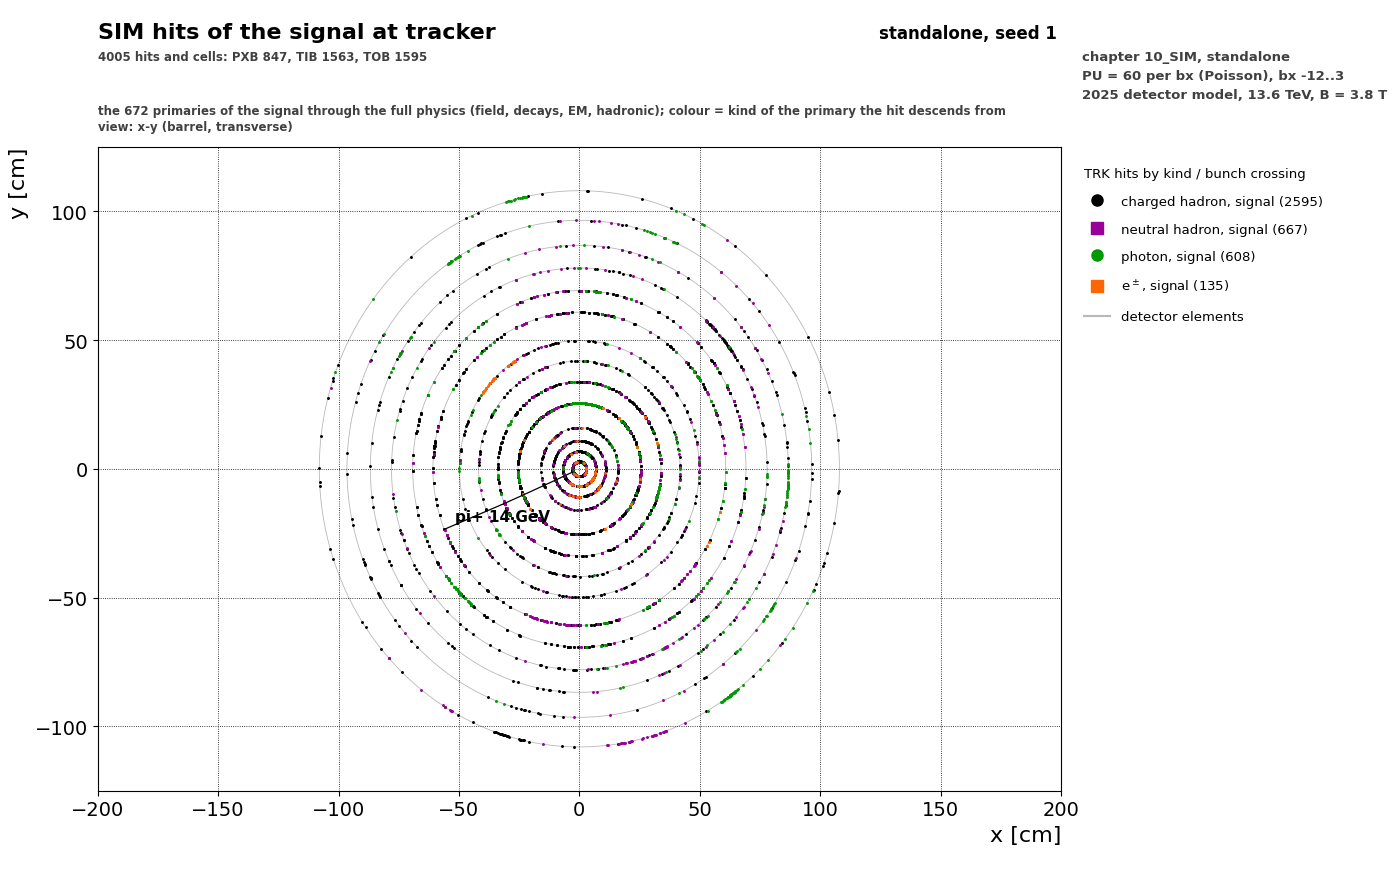
\includegraphics[width=0.495\textwidth]{SIM/Standalone/pages/simHits_signal_10_SIM_TRK_xy.png}\\[2pt]
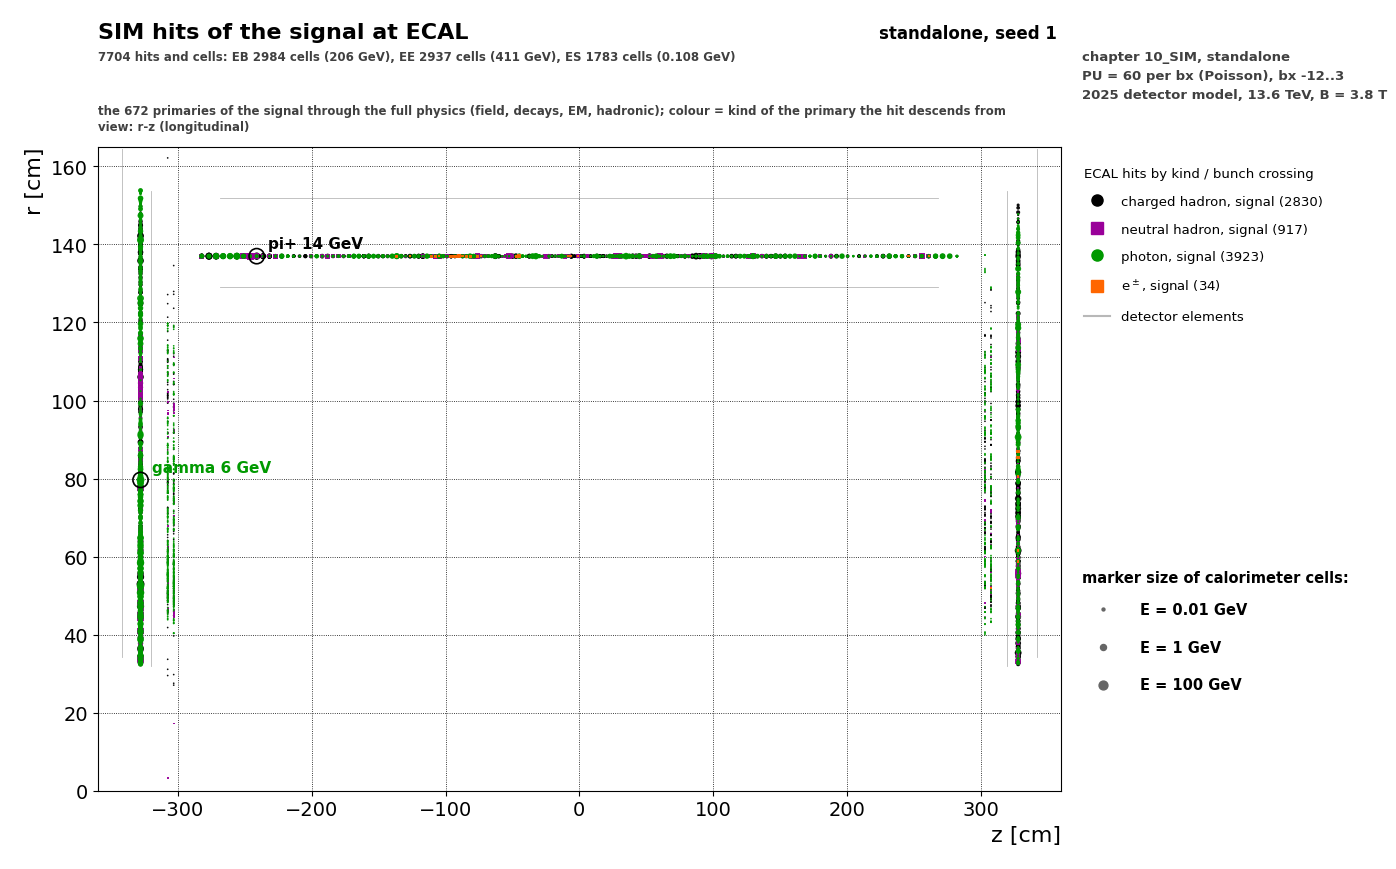
\includegraphics[width=0.495\textwidth]{SIM/Standalone/pages/simHits_signal_10_SIM_ECAL_rz.png}\hfill
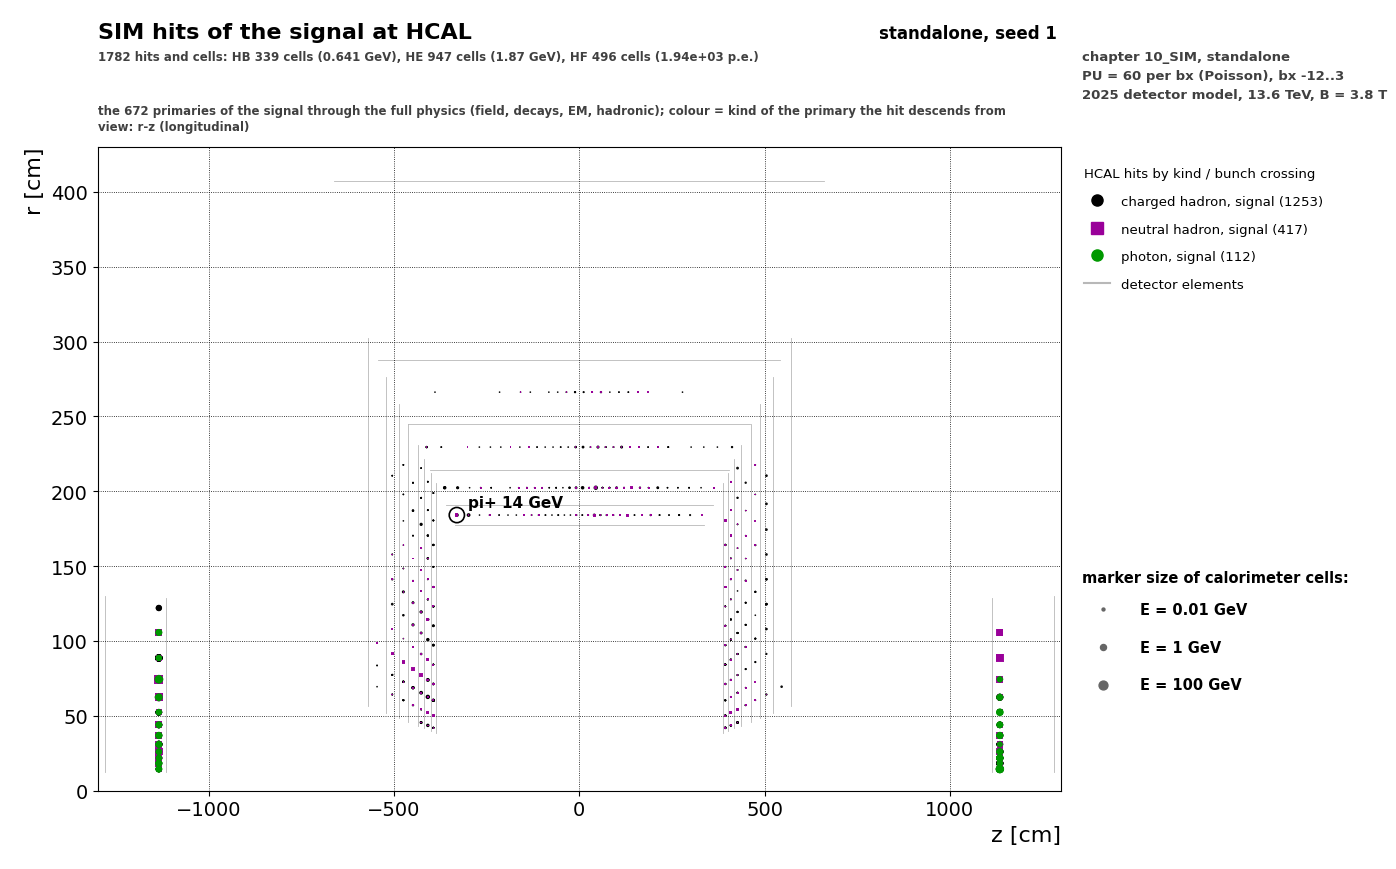
\includegraphics[width=0.495\textwidth]{SIM/Standalone/pages/simHits_signal_10_SIM_HCAL_rz.png}
\caption[The family station by station]{The family station by station
(\file{plot_simhits_SIM.py}). Top: the tracker in $r$--$z$ and its barrel in
$x$--$y$; bottom: ECAL and HCAL in $r$--$z$. A hit takes the colour of the
kind of primary it descends from: black charged hadrons, purple neutral
hadrons, green photons, orange electrons. The leading charged member of our
jet and the hardest photon are joined hit by hit.}
\label{fig:crowd_at_the_border:stations_signal}
\end{figure}

\begin{figure}[htbp]\centering
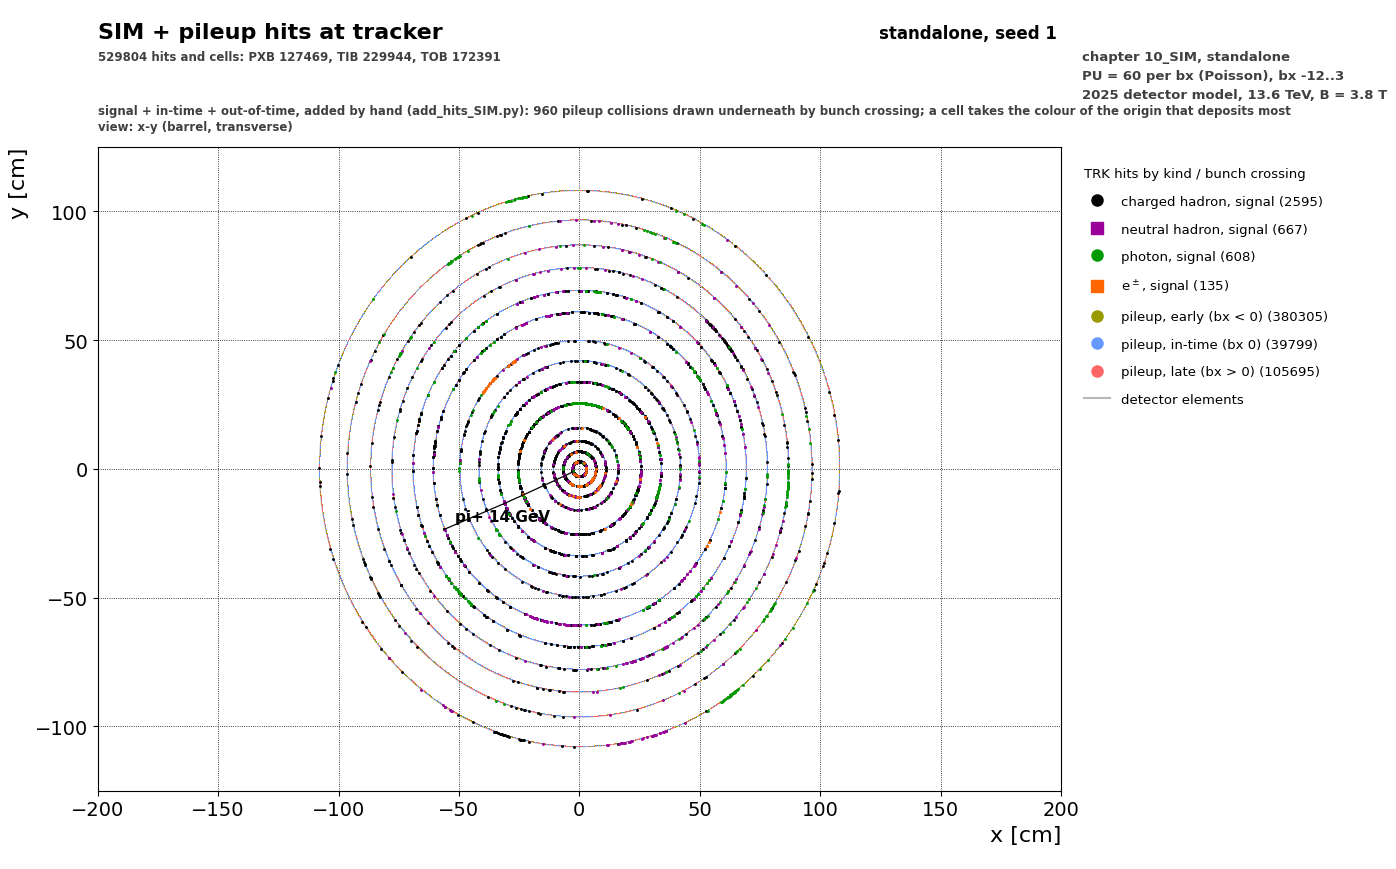
\includegraphics[width=0.495\textwidth]{SIM/Standalone/pages/simHits_mixed_10_SIM_TRK_xy.png}\hfill
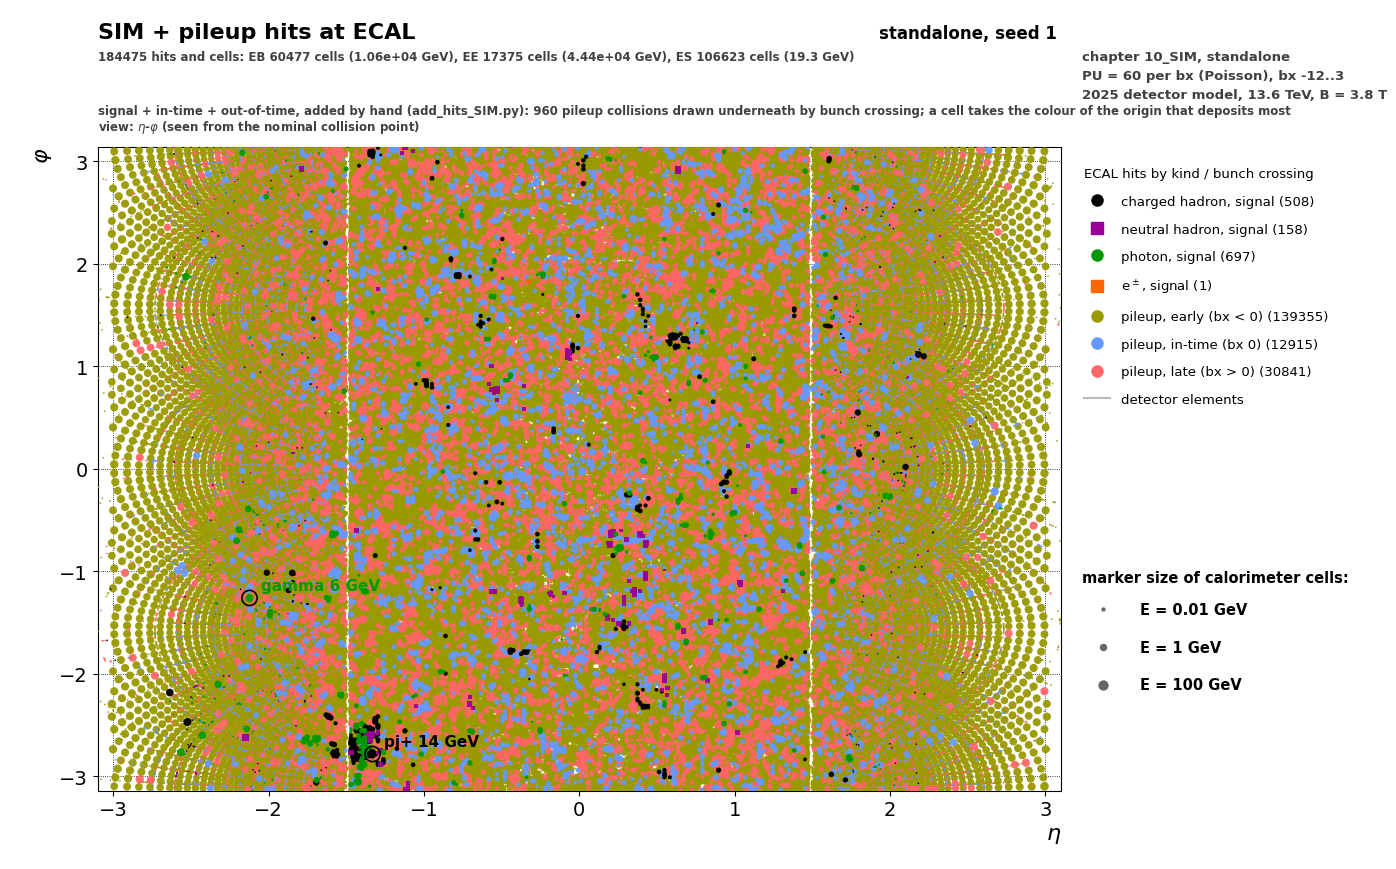
\includegraphics[width=0.495\textwidth]{SIM/Standalone/pages/simHits_mixed_10_SIM_ECAL_etaphi.png}\\[2pt]
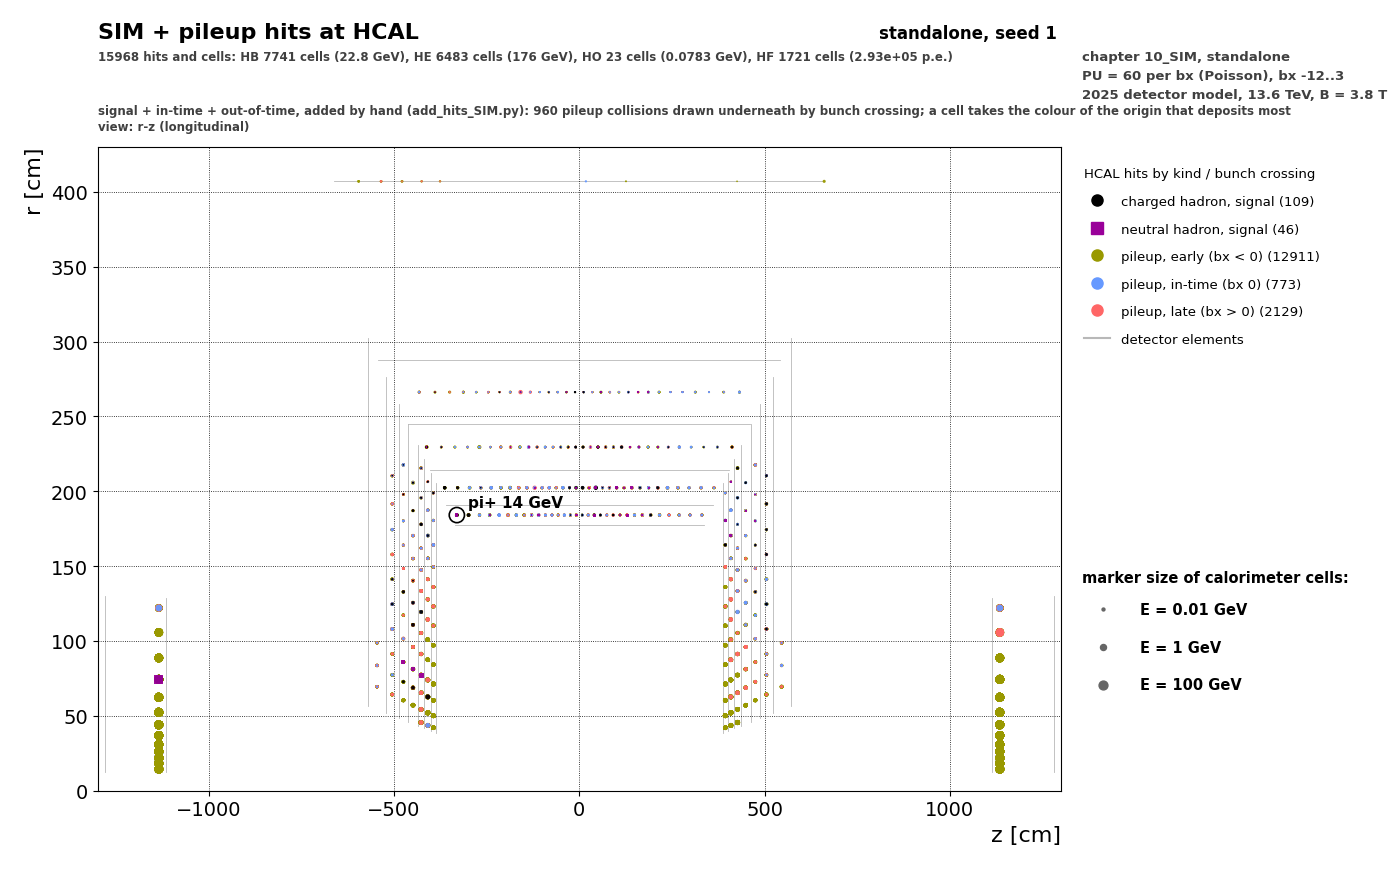
\includegraphics[width=0.495\textwidth]{SIM/Standalone/pages/simHits_mixed_10_SIM_HCAL_rz.png}\hfill
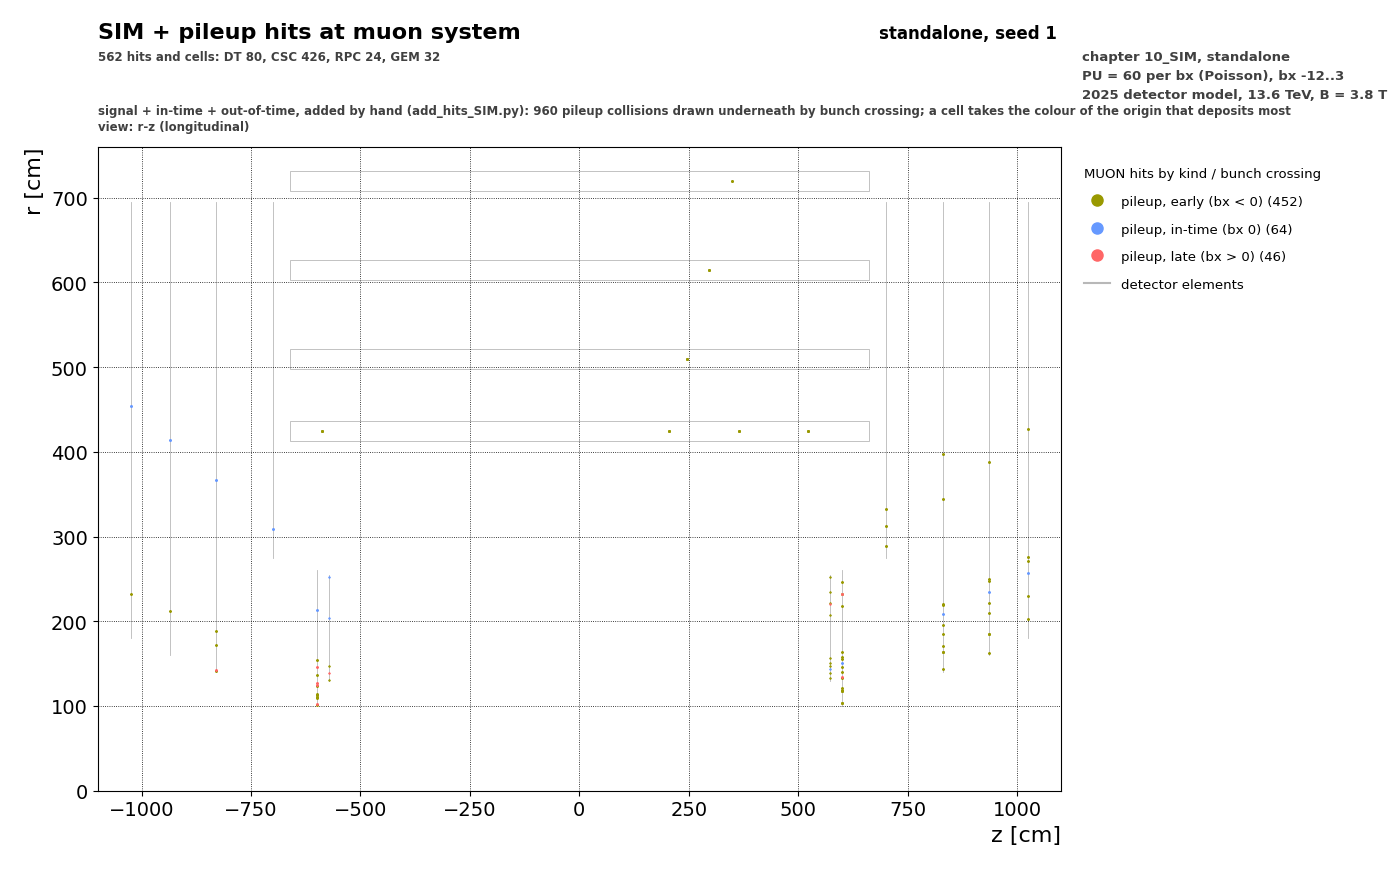
\includegraphics[width=0.495\textwidth]{SIM/Standalone/pages/simHits_mixed_10_SIM_MUON_rz.png}
\caption[The sum station by station]{The sum station by station: the
tracker barrel in $x$--$y$, the ECAL in $\eta$--$\phi$, the HCAL and the
muon system in $r$--$z$. The crowd is drawn underneath by bunch crossing,
olive early, blue in time, red late; a cell takes the colour of whoever
deposits most in it.}
\label{fig:crowd_at_the_border:stations_mixed}
\end{figure}

\paragraph{Our jet.}
\Cref{tab:crowd_at_the_border:ledger} follows the photograph of
\cref{ch:family_photograph} across the border. Its $31$ members carry
$222.8\GeV$ towards $\eta=-1.44$, the corner where the barrel meets the
endcap. Only $13$ of them reach the calorimeters as themselves, with
$44.3\GeV$ of vector \pt: ten photons converted, seven hadrons interacted in
the tracker, the $K^0_S$ decayed. Nothing is lost by that; the energy
arrives as secondaries. What is lost shows in the next row: the cells
record $133.5\GeV$ in $942$ crystals and $0.31\GeV$ in the scintillator of
$151$ HCAL cells, $46\GeV$ after the sampling factor, and their vector sum
is $73.5\GeV$ of the $99.8$. The difference is the physics of
\cref{sec:crowd_at_the_border:hadronic}: invisible energy, the response of
the calorimeters to hadrons, loopers that never arrive, and the gap between
barrel and endcap that this jet happens to point at.
\Cref{tab:crowd_at_the_border:circle} then counts everything the detector
receives inside the circle of the jet.

\begin{ledgerboth}{The Crossing of the Border}{tab:crowd_at_the_border:ledger}{From
the third row on, \pt is the vector sum of calorimeter cells seen from the
collision point, HCAL cells multiplied by the sampling factors of
\cref{ch:customs_form} ($125$ barrel, $190$ endcap), and
$n_{\mathrm{const}}$ counts cells. The \CMSSW rows follow its $b$ system, the
visible descendants of the $B^-$.}
\ledgerblock{Standalone (seed 1, \file{event_SIM.lhe})}
\ledgerrow{the photograph, \akfour jet [0], handed to \GEANT (chapter 9)}{99.83}{14.83}{31}{--}
\ledgerrow{its members reaching the calorimeters as primaries}{44.32}{--}{13}{$-55.51$}
\ledgerrow{what the cells record of its members and their secondaries}{73.52}{--}{1093}{$+29.20$}
\ledgerrow{all cells of the family in the circle $\Delta R<0.4$}{65.21}{--}{560}{$-8.31$}
\ledgerrow{\quad with the in-time crowd}{80.41}{--}{--}{$+15.20$}
\ledgerrow{\quad with the early crowd, $\bx=-12\ldots-1$}{247.03}{--}{--}{$+166.62$}
\ledgerrow{\quad with the late crowd, $\bx=+1\ldots+3$}{291.97}{--}{1655}{$+44.94$}
\ledgerblock{\CMSSW (run 1, event 1)}
\ledgerrow{the photograph, \akfour jet [0] (chapter 7)}{117.79}{16.72}{24}{--}
\ledgerrow{the $b$ system handed to \GEANT (chapter 9)}{56.82}{--}{8}{--}
\ledgerrow{its members reaching the calorimeters as primaries}{24.4}{--}{3}{$-32.4$}
\end{ledgerboth}

\begin{table}[htbp]\centering\footnotesize\setlength{\tabcolsep}{4pt}
\caption[The circle of our jet, by origin]{The circle of our jet,
$\Delta R<0.4$ around $(\eta,\phi)=(-1.44,-2.71)$: tracker hits, crystals
with energy, their energy and transverse energy, HCAL cells, the energy in
their scintillator and its transverse energy after the sampling factor, and
the sum of the two transverse energies, in GeV.}
\label{tab:crowd_at_the_border:circle}
\begin{tabular}{@{}lrrrrrrrr@{}}\toprule
 & tracker & \multicolumn{3}{c}{crystals} & \multicolumn{3}{c}{HCAL} & $\sum E_T$ \\
 & hits & cells & $E$ & $E_T$ & cells & $E_{\mathrm{scint}}$ & $E_T\times$factor & \\ \midrule
\simCircleRows
\bottomrule
\end{tabular}
\end{table}

\paragraph{The same event in \CMSSW.}
\label{sec:crowd_at_the_border:cmssw_event}
The companion runs \GEANT itself, four times on the signal with one
ingredient more each time, once on a library of $1000$ minimum-bias
collisions, and then the \Mix without its digitisers on $995$ of them.
Its stage table reads like ours: the primaries reaching the boundary fall
from $557$ to $310$ of $571$, the secondaries grow to $1355$, the tracker
hits from $6734$ to $10\,272$ with $2.33\GeV$ of energy loss, and the muon
chambers fill with $522$ hits when hadrons can ionise but not interact. Its
$b$ system, eight primaries with $140.3\GeV$ pointing at the endcap, reaches
the boundary with three of them and $24.4\GeV$ of \pt, and leaves
$63.6\GeV$ in the crystals and $0.39\GeV$ in the scintillator, about
$73\GeV$ after the sampling factor: half in each calorimeter, as for our
jet. One of its photons, $44\GeV$, is the lesson of
\cref{fig:crowd_at_the_border:shower} in a single particle: unconverted in
one run, it puts two thirds of its energy in one crystal; converted in the
first pixel layer in another, it lights $466$. In the sum the signal is
$0.49\,\%$ of $2.1$ million tracker hits and keeps $699$ of its $12\,804$
ECAL cells. The displays of \cref{fig:crowd_at_the_border:displays} are the
two events at this stage.

\begin{figure}[p]\centering
\ledgerdisplays
  {SIM/Standalone/pages/simHits_mixed_10_SIM_ALL_etaphi.png}
  {Standalone: the family with the $960$ collisions of its crowd underneath (\file{plot_simhits_SIM.py}).}
  {fig:crowd_at_the_border:journey}
  {SIM/CMSSW/simHits_mixed_10_SIM_ALL_etaphi_run1_event1.png}
  {\CMSSW: the signal with its $995$ pileup collisions, the \code{SimHitAnalyzer} page of \code{JitJetSW}.}
  {fig:crowd_at_the_border:cmssw}
\caption[The simulated hits in the $(\eta,\phi)$ plane, standalone and
\CMSSW]{Every simulated hit and cell in the $(\eta,\phi)$ plane, standalone
(a) and \CMSSW (b): the family by kind of primary, the crowd by bunch
crossing (olive early, blue in time, red late), cells sized by energy. In
both the family survives as the strings of its charged tracks and the cores
of its jets, ours at $(-1.4,-2.7)$ in (a).}
\label{fig:crowd_at_the_border:displays}
\end{figure}

\subsection{What this stop is, and what it is not}
\label{sec:crowd_at_the_border:caveats}
\begin{itemize}
  \item \textbf{A simulation in the spirit of \GEANT, not \GEANT.} The
    detector is $54$ surfaces and seven kinds of cells; a shower is a
    parametrised cloud of spots, a nuclear interaction in the tracker a toy
    model of pions and nucleons. The material is tuned to the CMS geometry;
    the calorimeter constants ($h/e$, the sampling fractions, the
    photoelectrons per \GeV of the HF) are chosen to give the scale of
    test beams and of the companion, not derived.
  \item \textbf{Fewer soft hits than \GEANT.} The script creates no
    $\delta$ rays, no Compton electrons and no nuclear fragments, and stops
    a particle below $10\MeV$. It has $12.8$ tracker hits per primary where
    \GEANT has $18.0$, and counts as hit only cells that received a spot of
    a few \MeV, where \GEANT keeps every deposit above $15\keV$. Cell
    counts of the two are not comparable; energies are.
  \item \textbf{The field is a box.} $3.8$~T inside $|z|<6.5$~m and nothing
    outside; the return field in the yoke, which bends muons back, is not
    there, and a muon flies straight from the HCAL to its stations.
  \item \textbf{SimHits are energy, not signals.} No pulse shape, no noise,
    no threshold, no time window: all sixteen crossings are in the sum with
    equal weight. The $231\GeV$ of the crowd in our circle is what the
    detector receives, not what it will read out.
  \item \textbf{One event is one sample}, and the two events of the stop are
    different events.
\end{itemize}

\section{Further reading}
\label{sec:crowd_at_the_border:further_reading}
The physics of this stop is the review of the passage of particles through
matter of the Particle Data Group~\cite{ParticleDataGroup:2024cfk}, and for
calorimeters the book of Wigmans~\cite{Wigmans:2000vf} and the review of
Fabjan and Gianotti~\cite{Fabjan:2003aq}. The detector is described
in~\cite{CMS:2008xjf,CMS:2024aqx}, its tracker material as measured with
nuclear interactions in~\cite{CMS:2018wqs}, the response of its barrel
calorimeters to hadrons in~\cite{USCMS:2009fxn}. The simulation of CMS with
\GEANT, its physics list and its validation are
in~\cite{CMS:2021dly,Srimanobhas:2024nmy,Banerjee:2017bhj}, the models
behind the list in~\cite{Wright:2015xia}, the fast simulation
in~\cite{Abdullin:2011zz,Rahmat:2011xp}, the mixing and premixing
in~\cite{Hildreth:2017caz}.

\begin{pitfalls}
\begin{itemize}[nosep]
  \item \emph{``A particle below $0.7\GeV$ leaves no energy in the
    calorimeter.''} It leaves none in the barrel. It spirals to the endcap
    and arrives there, late and far from where it was aimed.
  \item \emph{``The primaries at the boundary fell from $672$ to $407$, so a
    third of the energy is lost.''} The count is of particles that arrive
    as themselves. A converted photon arrives as two electrons with all of
    its energy.
  \item \emph{``The HCAL holds $2.5\GeV$, so the hadrons deposit almost
    nothing.''} A SimHit of a sampling calorimeter is the energy in the
    scintillator, about $1\,\%$ of what the calorimeter absorbed. And an HF
    hit is not an energy at all but a number of photoelectrons.
  \item \emph{Radiation length and interaction length are different units.}
    The crystals are $26\,\Xzero$ but $1.1\,\lamI$ deep: a wall for a
    photon, a window for one pion in three.
  \item \emph{Is the signal simulated together with its pileup?} Never. They
    meet at the level of hits here, and in the production one step later,
    as digitised signals (premixing).
  \item \emph{``Out-of-time pileup is out of the event.''} At this stop it
    is three quarters of the event. The electronics decide how much of it
    stays.
\end{itemize}
\end{pitfalls}

\begin{exercises}
\item From \cref{eq:crowd_at_the_border:looper}: what field would let a
  pion of $0.3\GeV$ reach the barrel ECAL? Run
  \code{standalone\_SIM.py --sample signal --field 2 -v} and compare the
  loopers and the tracker hits with the $3.8$~T run.
\item Run the family with \code{--stage B\_Decay\_EM} and explain the $955$
  muon-chamber hits. Which hadrons make them, and why are they gone in the
  full simulation?
\item From the primary listing of \file{event_SIM.lhe}, take the photons
  above $1\GeV$ in $|\eta|<1$ and in $1.5<|\eta|<2.5$ and count the
  conversions. Deduce the material in each region with
  \cref{eq:crowd_at_the_border:conversion} and compare with
  \cref{fig:crowd_at_the_border:material}.
\item With \cref{eq:crowd_at_the_border:fem}, compute the response
  $f_{em}+(1-f_{em})h/e$ for one pion of $100\GeV$ and for ten pions of
  $10\GeV$. Which jet looks more energetic to the calorimeter?
\item In \file{add_hits_SIM.py}, set the shift to zero and compare the time
  distribution of the tracker hits with \cref{fig:crowd_at_the_border:time}.
  Then keep only the crossings $\bx=-3\ldots+3$, the Phase-2 window of the
  release, and recompute the circle of our jet.
\item For the HL-LHC, scale the in-time column of
  \cref{tab:crowd_at_the_border:hits_ledger} to $200$ collisions. How many
  tracker hits per crossing, and what share is the family's?
\end{exercises}

\subsection*{Open problems in the context of Phase-2 LHC}
\label{sec:crowd_at_the_border:open_problems}
\begin{enumerate}
  \item \textbf{The CPU budget of full simulation.} The move to Run~3 gained
    about $25\,\%$ in speed~\cite{CMS:2021dly}; the plan for Phase-2 is, in
    the words of the collaboration, very ambitious~\cite{Srimanobhas:2024nmy,Srimanobhas:2025abv},
    and the community asks for large factors~\cite{HEPSoftwareFoundation:2018fmg,Apostolakis:2022nnf}
    within a computing model that is itself being
    revised~\cite{Perez-CaleroYzquierdo:2026dvu}. Our crowd costs $140$ times
    the family at $60$ collisions and sixteen crossings; at $200$ the ratio
    more than triples.
  \item \textbf{A calorimeter of six million channels.} The HGCAL~\cite{CMS:2017jpq}
    replaces the endcap crystals and tiles of this chapter by silicon pads
    and small tiles in $47$ layers. Its prototypes agree with \GEANT for
    positrons and pions of $20$ to $300\GeV$~\cite{CMSHGCAL:2021nyx,CMS:2022jvd},
    the first such test of hadronic showers at this granularity; whether the
    physics list describes the substructure of a shower, and at what cost
    per event, is open.
  \item \textbf{Time as a fourth coordinate.} The timing layer~\cite{Butler:2019rpu}
    aims at $30$ to $40$~ps per track and needs hit times simulated to that
    precision~\cite{Sorrentino:2023hjw}. The time structure of a hadronic
    shower depends on its slow neutrons~\cite{CALICE:2014tgv}, the part of
    the physics that fast physics lists cut first, and that this chapter
    called invisible.
  \item \textbf{The hadronic models and the jet energy scale.} Single-hadron
    response in data and \GEANT differs by up to $5\,\%$, which becomes a
    jet-scale uncertainty of $2$ to $5\,\%$ for the hardest
    jets~\cite{ATLAS:2016djy}. Tunes of the hadronic models with
    uncertainties are only beginning~\cite{Genser:2023fic}; no uncertainty
    model exists for a new calorimeter before it takes data.
  \item \textbf{Transport on graphics processors.} Electromagnetic
    transport runs $6$ to $32$ times faster on a GPU, but a full application
    with hadronic physics gains only a factor of about
    two~\cite{Johnson:2024qqt}, and the first integrations into experiment
    frameworks met difficulties~\cite{Apostolakis:2025vca}; the options of
    \GEANT~11 for faster electromagnetic physics are being
    adopted~\cite{Hahnfeld:2024zrb}.
  \item \textbf{Learning the simulation.} Machine-learned refinement of the
    fast simulation~\cite{Bein:2023ylt}, generative calorimeter
    showers~\cite{Amram:2023onf,Krause:2024avx} and end-to-end models that
    skip the hits altogether~\cite{Vaselli:2024vrx,Vaselli:2025fov} are
    orders of magnitude faster. How to validate them, and what systematic
    uncertainty to assign to a jet they produced, is unsolved; and a model
    that skips the hits cannot answer the question of this chapter, whose
    hit it was.
  \item \textbf{The premixed crowd at 200.} The production digitises the
    crowd once and reuses it~\cite{Hildreth:2017caz}. The release mixes
    seven crossings of $200$ for Phase-2, $1400$ collisions per event; how
    large the premixed library must be, and what its reuse does to
    correlations between events, has not been quantified in a publication we
    could find.
\end{enumerate}
The family has crossed, and so has everyone else. The next stop turns what
the country received into numbers on a form.

%% ---------------------------------------------------------------------------
% Chapter 11: The Customs Form: Digitisation
% SKELETON (2026-11-15), laid out after Constitution.md rules B-E. Every
% \todo marks text, numbers or figures still to come.
% The scripts, records, logs and films of this stop will live in example/DIGI/,
% the technical companion is chapter/chapter_11_DIGI.md, and the CMSSW side
% (the DIGI step of the mixed event) is chapter 11 of JitJetSW, linked from
% example/DIGI/CMSSW/README.md.
% What this stop is: the SimHits of the family and the crowd become what
% the electronics write: charge, pulses sampled every 25 ns, pedestals and
% noise, ADC counts, zero suppression. Energy is added (noise, out-of-time
% pulses) and removed (thresholds). The checkpoints read the result.
% ---------------------------------------------------------------------------
%% chapter-local shorthands
\providecommand{\placeholderfig}[1]{\fbox{\parbox[c][4cm][c]{0.9\textwidth}{\centering\todo{#1}}}}
\providecommand{\bx}{\ensuremath{\mathrm{bx}}\xspace}
\providecommand{\ns}{\ensuremath{\,\mathrm{ns}}\xspace}
\providecommand{\Npe}{\ensuremath{N_{\mathrm{pe}}}\xspace}
\chapter{The Customs Form: Digitisation}
\chaptermark{The Customs Form}
\label{ch:customs_form}

\begin{journeybox}
The weighing is over, and now it has to be written down. The customs form
has boxes of fixed size, its own units and its own rounding; a small item
is not worth a line and is left off, the clerk's hand trembles a little on
every entry, and the ink of the previous traveller has not dried on the
page. What travels on is not the luggage but the form. \todo{Polish the
metaphor paragraph (B1).}
\end{journeybox}

\physicsline{from deposited energy to charge: light yield, photostatistics,
gains and saturation; the pulse and the $25\ns$ clock, and the out-of-time
crowd inside a pulse; pedestals, electronic noise and quantisation into ADC
counts; zero suppression and selective readout; the tracker's charge
sharing and thresholds. The one number to take away: \todo{the energy of
our jet in digitised cells above threshold, against the SimHits of
\cref{ch:crowd_at_the_border}}.}

\section{What we will see at this stop}
\label{sec:customs_form:what_we_compute}

% (C1-1) motivation, connected to the previous chapter
\todo{Motivation (C1-1). \Cref{ch:crowd_at_the_border} ended with energy in
the active volumes, the family's and the crowd's added together. No
detector reads energy: it reads light or charge, shaped into a pulse,
sampled by the clock and written in counts. This stop is the conversion,
and the first place where the event is what the real detector writes.
Give the four numbers to take away.}

\paragraph{The film.}
\label{sec:customs_form:animation}
% (C1-2) one paragraph, at most one figure of key frames
\todo{One paragraph on the eleventh film of the playlist of \jitjetworld.}

\begin{figure}[htbp]\centering
\placeholderfig{Key frames of the film, from
\file{example/DIGI/Standalone/animate_standalone_DIGI_stills.pdf}.}
\caption[Key frames of the animated digitisation stage]{Key frames of the
animated digitisation stage. \todo{Caption.}}
\label{fig:customs_form:stills}
\end{figure}

\paragraph{The picture to carry: one cell, from energy to counts.}
% (C1-3) a sketch or diagram
\todo{The picture to carry: one ECAL crystal and one HCAL tower of our jet,
the energy turned into photoelectrons, the pulse with the out-of-time
pulses under it, the ten samples, the pedestal and the counts written.
TikZ in \file{chapter/tikz/digi_*.tex}.}

\begin{figure}[htbp]\centering
\placeholderfig{TikZ: one cell from energy to ADC counts
(\file{chapter/tikz/digi_pulse.tex}).}
\caption[The customs form]{The customs form. \todo{Caption.}}
\label{fig:customs_form:pulse_sketch}
\end{figure}

\paragraph{The number, three ways.}
\label{sec:customs_form:validation}
% (C1-4) the agreement table, one or two paragraphs
\todo{One or two paragraphs on the agreement table: the standalone script
(the digitisers ported to NumPy), the official package (the digitiser
models with the 2024 conditions), and \CMSSW (the DIGI step of JitJetSW).
How each column is produced is in the companion,}
\begin{center}
  \companion{chapter_11_DIGI}
\end{center}

\begin{table}[htbp]\centering\small
\caption[The customs form obtained three ways]{The customs form obtained
three ways. \todo{Caption: what each column is.}}
\label{tab:customs_form:numbers}
\begin{tabular}{lrrr}\toprule
 & standalone & official & \CMSSW 2024 \\ \midrule
photoelectrons per GeV: ECAL / HCAL & \todo{} & \todo{} & \todo{} \\
noise per channel [MeV] & \todo{} & \todo{} & \todo{} \\
out-of-time energy in our jet's pulses [GeV] & \todo{} & \todo{} & \todo{} \\
channels read out after zero suppression & \todo{} & \todo{} & \todo{} \\
energy lost below threshold in our jet [GeV] & \todo{} & \todo{} & \todo{} \\
tracker clusters in our jet & \todo{} & \todo{} & \todo{} \\
\bottomrule
\end{tabular}
\end{table}

\section{Let us dive into the details: the theory}
\label{sec:customs_form:theory}
% Every subsection: (C2-1) motivation, (C2-2) TikZ sketch, (C2-3) equation,
% (C2-4) numbers for our event from the -v log, inline, (C2-5) one plot.

\subsection{From energy to charge: light, photoelectrons and gains}
\label{sec:customs_form:charge}
\todo{(C2-1) The crystal makes light, the scintillator makes light, the
silicon makes charge; each conversion counts quanta and fluctuates.
(C2-2) TikZ: crystal, photodetector and preamplifier.
(C2-3) $\Npe=E\cdot Y$ and the photostatistics term $\sigma/E=1/\sqrt{\Npe}$;
the saturation of a SiPM.
(C2-4) Numbers from the \code{-v} log.
(C2-5) Plot: the photostatistics term against energy.}

\subsection{The pulse and the clock}
\label{sec:customs_form:pulse}
\todo{(C2-1) A hit is a pulse that lasts longer than $25\ns$, and the pulses
of the crossings before ours sit under it.
(C2-2) TikZ: the pulse and its samples, with the out-of-time pulses.
(C2-3) The pulse shape $f(t)$ and the sampled amplitude
$S_i=\sum_{\bx}A_{\bx}\,f(t_i-25\ns\cdot\bx)$.
(C2-4) Numbers from the \code{-v} log.
(C2-5) Plot: the ten samples of the hottest crystal of our jet.}

\subsection{Pedestals, noise and ADC counts}
\label{sec:customs_form:noise}
\todo{(C2-1) The form has boxes of fixed size and the clerk's hand trembles.
(C2-2) TikZ: the pedestal, the noise band and the ADC steps.
(C2-3) The quantisation noise $q/\sqrt{12}$, the electronic noise and the
gain switching.
(C2-4) Numbers from the \code{-v} log.
(C2-5) Plot: the noise of our jet's channels.}

\subsection{What is not written: zero suppression and selective readout}
\label{sec:customs_form:zero_suppression}
\todo{(C2-1) Most channels hold noise, and writing them all is impossible.
(C2-2) TikZ: the selective readout regions around our jet.
(C2-3) The threshold $n\sigma_{\mathrm{noise}}$ and the energy lost below it.
(C2-4) Numbers from the \code{-v} log.
(C2-5) Plot: the energy lost against the threshold.}

\subsection{The tracker: charge sharing and clusters}
\label{sec:customs_form:tracker}
\todo{(C2-1) A charged member crossing silicon leaves charge on several
pixels or strips.
(C2-2) TikZ: drift, Lorentz angle and charge sharing.
(C2-3) The Lorentz drift $\tan\theta_L=\mu_H B$ and the cluster position.
(C2-4) Numbers from the \code{-v} log.
(C2-5) Plot: the cluster sizes of our jet's tracks.}

\paragraph{The recipe.}
\todo{The recipe, step by step, that the standalone script runs.}

\section{The energy ledger: our jet at this stage}
\label{sec:customs_form:ledger}
% (C3-1) the ledger table, "The same event in CMSSW", one figure page
\todo{What the record \file{example/DIGI/event_DIGI.*} holds, and what the
ledger says.}

\begin{ledgerboth}{The Customs Form}{tab:customs_form:ledger}{%
\todo{What the two blocks are.}}
\ledgerblock{Standalone (seed 1)}
\ledgerrow{the photograph, \code{ak4GenJets} jet [0] (chapter 7)}{99.83}{14.83}{31}{--}
\ledgerrow{with the crowd's SimHits (chapter 10)}{\todo{}}{--}{\todo{}}{\todo{}}
\ledgerrow{digitised, above threshold}{\todo{}}{--}{\todo{}}{\todo{}}
\ledgerblock{\CMSSW (run 1, event 1)}
\ledgerrow{the photograph, \code{ak4GenJets} jet [0] (chapter 7)}{117.79}{16.72}{24}{--}
\ledgerrow{digitised, above threshold}{\todo{}}{--}{\todo{}}{\todo{}}
\end{ledgerboth}

\paragraph{The same event in \CMSSW.}
\label{sec:customs_form:cmssw_event}
\todo{The DIGI step of JitJetSW: the digis of our jet, read from the log of
the analyser.}

\begin{figure}[p]\centering
\placeholderfig{Standalone display: \file{DIGI/journey_DIGI.pdf}.}\\[2mm]
\placeholderfig{\CMSSW display: \file{DIGI/CMSSW/digiAnalyzer_11_DIGI.pdf}.}
% when the files exist:
% \ledgerdisplays
%   {DIGI/journey_DIGI.pdf}{Standalone: ...}{fig:customs_form:journey}
%   {DIGI/CMSSW/digiAnalyzer_11_DIGI.pdf}{\CMSSW: ...}{fig:customs_form:cmssw}
\caption[The digitised event, standalone and \CMSSW]{The digitised event,
standalone (top) and \CMSSW (bottom). \todo{Caption.}}
\label{fig:customs_form:displays}
\end{figure}

\subsection{What this stop is, and what it is not}
\label{sec:customs_form:caveats}
\begin{itemize}
  \item \todo{Digis are counts, not energies: turning them back into
    energy is the local reconstruction of \cref{ch:footprints}.}
  \item \todo{The conditions are the 2024 ones, one set for the whole year.}
  \item \todo{One event is one sample.}
\end{itemize}

\section{Further reading}
\label{sec:customs_form:further_reading}
The signal amplitudes of the ECAL and their reconstruction are in
\cite{CMS:2020uim}, its calibration and resolution in \cite{CMS:2013lxn};
the Run-3 electronics of the calorimeters, including the SiPM readout of the
HCAL, are in \cite{CMS:2024aqx}, and calorimetry in general in
\cite{Wigmans:2000vf}. \todo{Literature survey: the HCAL and tracker
digitisers, selective readout.}

\begin{pitfalls}
\begin{itemize}[nosep]
  \item \todo{Pitfall 1.}
  \item \todo{Pitfall 2.}
\end{itemize}
\end{pitfalls}

\begin{exercises}
\item \todo{Exercise 1.}
\item \todo{Exercise 2.}
\end{exercises}

\subsection*{Open problems in the context of Phase-2 LHC}
\label{sec:customs_form:open_problems}
\todo{Literature survey: the Phase-2 front ends, the high-granularity
calorimeter~\cite{CMS:2017jpq}, the Phase-2 tracker~\cite{CMS:2017lum}
and timing~\cite{Butler:2019rpu}.}
\begin{enumerate}
  \item \todo{Open problem 1.}
  \item \todo{Open problem 2.}
\end{enumerate}
The next stop is the first checkpoint, where the form is read in a hurry.

%% ---------------------------------------------------------------------------
% Chapter 12: The First Checkpoint: Level-1 Trigger
% SKELETON (2026-11-15), laid out after Constitution.md rules B-E. Every
% \todo marks text, numbers or figures still to come.
% The scripts, records, logs and films of this stop will live in example/L1T/,
% the technical companion is chapter/chapter_12_L1T.md, and the CMSSW side
% (the L1 emulation of the digitised event) is chapter 12 of JitJetSW,
% linked from example/L1T/CMSSW/README.md.
% What this stop is: a checkpoint. Nothing is added to the event or taken
% from it; the event is stamped, accepted or not, with the L1 seeds it fired.
% ---------------------------------------------------------------------------
%% chapter-local shorthands
\providecommand{\placeholderfig}[1]{\fbox{\parbox[c][4cm][c]{0.9\textwidth}{\centering\todo{#1}}}}
\providecommand{\us}{\ensuremath{\,\mu\mathrm{s}}\xspace}
\chapter{The First Checkpoint: Level-1 Trigger}
\chaptermark{The First Checkpoint}
\label{ch:first_checkpoint}

\begin{journeybox}
At the first checkpoint a guard with a coarse ledger has a few microseconds
to decide whether the family may continue at all. He sees only towers, not
people, and his thresholds are the first place where families are lost with
a probability rather than a certainty. Those who pass get a stamp that says
which rule let them through. \todo{Polish the metaphor paragraph (B1).}
\end{journeybox}

\physicsline{forty million crossings per second and a hundred thousand
kept; trigger primitives and calorimeter trigger towers; Layer-1
calibration and Layer-2 jets of $9\times9$ towers; Level-1 pileup
subtraction; the global trigger menu, seeds and prescales; efficiency
turn-on curves. The one number to take away: \todo{the L1 jet of our
event against the jet of \cref{ch:family_photograph}, and the seed that
let it through}.}

\section{What we will see at this stop}
\label{sec:first_checkpoint:what_we_compute}

% (C1-1) motivation, connected to the previous chapter
\todo{Motivation (C1-1). \Cref{ch:customs_form} wrote the event as the
detector writes it, every crossing. Nothing can store forty million of
them a second: a decision has to be taken in a few microseconds, on
coarse information, by custom hardware. This stop is that decision for our
event. Give the four numbers to take away.}

\paragraph{The film.}
\label{sec:first_checkpoint:animation}
% (C1-2) one paragraph, at most one figure of key frames
\todo{One paragraph on the twelfth film of the playlist of \jitjetworld.}

\begin{figure}[htbp]\centering
\placeholderfig{Key frames of the film, from
\file{example/L1T/Standalone/animate_standalone_L1T_stills.pdf}.}
\caption[Key frames of the animated Level-1 stage]{Key frames of the
animated Level-1 stage. \todo{Caption.}}
\label{fig:first_checkpoint:stills}
\end{figure}

\paragraph{The picture to carry: the guard's ledger.}
% (C1-3) a sketch or diagram
\todo{The picture to carry: the towers of our event as the L1 calorimeter
trigger sees them, the $9\times9$ window around our jet, the pileup
estimate around it, and the menu with the seed that fired. TikZ in
\file{chapter/tikz/l1t_*.tex}.}

\begin{figure}[htbp]\centering
\placeholderfig{TikZ: trigger towers and the L1 jet window
(\file{chapter/tikz/l1t_towers.tex}).}
\caption[The first checkpoint]{The first checkpoint. \todo{Caption.}}
\label{fig:first_checkpoint:towers_sketch}
\end{figure}

\paragraph{The number, three ways.}
\label{sec:first_checkpoint:validation}
% (C1-4) the agreement table, one or two paragraphs
\todo{One or two paragraphs on the agreement table: the standalone script
(the Layer-1/Layer-2 jet algorithm and a menu ported to NumPy), the
official package (the L1 emulator with the 2025 menu), and \CMSSW (the L1
step of JitJetSW). How each column is produced is in the companion,}
\begin{center}
  \companion{chapter_12_L1T}
\end{center}

\begin{table}[htbp]\centering\small
\caption[The first checkpoint obtained three ways]{The first checkpoint
obtained three ways. \todo{Caption: what each column is.}}
\label{tab:first_checkpoint:numbers}
\begin{tabular}{lrrr}\toprule
 & standalone & emulator & \CMSSW 2025 \\ \midrule
trigger towers above threshold & \todo{} & \todo{} & \todo{} \\
L1 jets above $30\GeV$ & \todo{} & \todo{} & \todo{} \\
our L1 jet: $E_T$ [GeV], $\eta$, $\phi$ & \todo{} & \todo{} & \todo{} \\
pileup subtracted from our L1 jet [GeV] & \todo{} & \todo{} & \todo{} \\
$H_T$ [GeV] & \todo{} & \todo{} & \todo{} \\
seeds fired & \todo{} & \todo{} & \todo{} \\
\bottomrule
\end{tabular}
\end{table}

\section{Let us dive into the details: the theory}
\label{sec:first_checkpoint:theory}
% Every subsection: (C2-1) motivation, (C2-2) TikZ sketch, (C2-3) equation,
% (C2-4) numbers for our event from the -v log, inline, (C2-5) one plot.

\subsection{Forty million times per second: the Level-1 problem}
\label{sec:first_checkpoint:l1_problem}
\todo{(C2-1) Why a hardware trigger, and why so fast.
(C2-2) TikZ: the L1 data flow, calorimeter and muon paths to the global
trigger.
(C2-3) The rate $R=L\,\sigma_{\mathrm{eff}}$ and the latency budget.
(C2-4) Numbers from the \code{-v} log.
(C2-5) Plot: the rate against the jet threshold.}

\subsection{Trigger primitives and towers}
\label{sec:first_checkpoint:towers}
\todo{(C2-1) The guard sees towers, not crystals.
(C2-2) TikZ: crystals summed into a tower, ECAL and HCAL.
(C2-3) The tower transverse energy and its compression.
(C2-4) Numbers from the \code{-v} log.
(C2-5) Plot: the towers of our event.}

\subsection{The Level-1 jet: calibration and pileup subtraction}
\label{sec:first_checkpoint:l1_jet}
\todo{(C2-1) A jet in a few hundred nanoseconds.
(C2-2) TikZ: the $9\times9$ window and the surrounding strips used for the
pileup estimate.
(C2-3) The jet sum, the pileup subtraction and the calibration look-up
table.
(C2-4) Numbers from the \code{-v} log.
(C2-5) Plot: the L1 jet response against the jet of chapter 7.}

\subsection{Efficiency turn-on curves: the mathematics of a threshold}
\label{sec:first_checkpoint:turn_on}
\todo{(C2-1) A threshold on a smeared quantity is a probability.
(C2-2) TikZ: a threshold on the L1 scale seen on the offline scale.
(C2-3) $\varepsilon(\pt)=\frac12\left[1+\mathrm{erf}\left(\frac{\pt-\mu}{\sqrt2\,\sigma}\right)\right]$.
(C2-4) Numbers from the \code{-v} log.
(C2-5) Plot: the turn-on of the seed our event fired.}

\subsection{The menu: seeds and prescales}
\label{sec:first_checkpoint:menu}
\todo{(C2-1) The stamp says which rule let the family through.
(C2-2) TikZ: the global trigger as a list of conditions.
(C2-3) The prescaled rate $R/P$ and the total within the budget.
(C2-4) Numbers from the \code{-v} log.
(C2-5) Plot: the seeds of the menu our event fired.}

\paragraph{The recipe.}
\todo{The recipe, step by step, that the standalone script runs.}

\section{The energy ledger: our jet at this stage}
\label{sec:first_checkpoint:ledger}
% (C3-1) the ledger table, "The same event in CMSSW", one figure page
\todo{What the record \file{example/L1T/event_L1T.*} holds, and what the
ledger says: this stop adds and removes nothing; the L1 jet is a coarse
copy, and the stamp is the decision.}

\begin{ledgerboth}{The First Checkpoint}{tab:first_checkpoint:ledger}{%
\todo{What the two blocks are.}}
\ledgerblock{Standalone (seed 1)}
\ledgerrow{the photograph, \code{ak4GenJets} jet [0] (chapter 7)}{99.83}{14.83}{31}{--}
\ledgerrow{digitised, above threshold (chapter 11)}{\todo{}}{--}{\todo{}}{\todo{}}
\ledgerrow{the L1 jet}{\todo{}}{--}{--}{\todo{}}
\ledgerblock{\CMSSW (run 1, event 1)}
\ledgerrow{the photograph, \code{ak4GenJets} jet [0] (chapter 7)}{117.79}{16.72}{24}{--}
\ledgerrow{the L1 jet}{\todo{}}{--}{--}{\todo{}}
\end{ledgerboth}

\paragraph{The same event in \CMSSW.}
\label{sec:first_checkpoint:cmssw_event}
\todo{The L1 emulation of JitJetSW on our event: the L1 jets, the sums and
the seeds, read from the log of the analyser.}

\begin{figure}[p]\centering
\placeholderfig{Standalone display: \file{L1T/journey_L1T.pdf}.}\\[2mm]
\placeholderfig{\CMSSW display: \file{L1T/CMSSW/l1tAnalyzer_12_L1T.pdf}.}
% when the files exist:
% \ledgerdisplays
%   {L1T/journey_L1T.pdf}{Standalone: ...}{fig:first_checkpoint:journey}
%   {L1T/CMSSW/l1tAnalyzer_12_L1T.pdf}{\CMSSW: ...}{fig:first_checkpoint:cmssw}
\caption[The event at Level~1, standalone and \CMSSW]{The event at
Level~1, standalone (top) and \CMSSW (bottom). \todo{Caption.}}
\label{fig:first_checkpoint:displays}
\end{figure}

\subsection{What this stop is, and what it is not}
\label{sec:first_checkpoint:caveats}
\begin{itemize}
  \item \todo{A checkpoint, not a measurement: the L1 jet is never used
    in an analysis, only its decision is.}
  \item \todo{The menu is the 2025 menu at one luminosity.}
  \item \todo{One event is one sample: the turn-on is the ensemble.}
\end{itemize}

\section{Further reading}
\label{sec:first_checkpoint:further_reading}
The trigger system of CMS is described in \cite{CMS:2016ngn} and the
performance of its Level-1 trigger in \cite{CMS:2020cmk}; the Run-3 state
of the detector and its trigger is in \cite{CMS:2024aqx}. \todo{Literature
survey: the Run-3 calorimeter trigger, the L1 pileup subtraction, the
2025 menu.}

\begin{pitfalls}
\begin{itemize}[nosep]
  \item \todo{Pitfall 1.}
  \item \todo{Pitfall 2.}
\end{itemize}
\end{pitfalls}

\begin{exercises}
\item \todo{Exercise 1.}
\item \todo{Exercise 2.}
\end{exercises}

\subsection*{Open problems in the context of Phase-2 LHC}
\label{sec:first_checkpoint:open_problems}
\todo{Literature survey: the Phase-2 Level-1 trigger~\cite{CMS:2020jkc},
tracks and particle flow at Level~1, $12.5\us$ of latency and $750$~kHz.}
\begin{enumerate}
  \item \todo{Open problem 1.}
  \item \todo{Open problem 2.}
\end{enumerate}
The next stop is the second checkpoint, where the family is looked at more
closely.

%% ---------------------------------------------------------------------------
% Chapter 13: The Second Checkpoint: High-Level Trigger
% SKELETON (2026-11-15), laid out after Constitution.md rules B-E. Every
% \todo marks text, numbers or figures still to come.
% The scripts, records, logs and films of this stop will live in example/HLT/,
% the technical companion is chapter/chapter_13_HLT.md, and the CMSSW side
% (the HLT menu run on the L1-accepted event) is chapter 13 of JitJetSW,
% linked from example/HLT/CMSSW/README.md.
% What this stop is: the second checkpoint. A fast reconstruction of the
% event, online jets and online corrections, and a decision: the paths the
% event fired, the stamp it carries into the stored data.
% ---------------------------------------------------------------------------
%% chapter-local shorthands
\providecommand{\placeholderfig}[1]{\fbox{\parbox[c][4cm][c]{0.9\textwidth}{\centering\todo{#1}}}}
\chapter{The Second Checkpoint: High-Level Trigger}
\chaptermark{The Second Checkpoint}
\label{ch:second_checkpoint}

\begin{journeybox}
The second checkpoint is staffed by the same kind of officers who will later
conduct the census, but in a hurry. They reconstruct the family quickly,
calibrate it with an older table, and keep only about one crossing in a
hundred of those the first guard let through. The family that passes
carries the stamps of both checkpoints into the archive. \todo{Polish the
metaphor paragraph (B1).}
\end{journeybox}

\physicsline{from a hundred kilohertz to a few kilohertz; the HLT farm and
its GPUs; paths, modules and filters; calorimeter jets and Particle-Flow
jets online; online pileup mitigation and online jet energy corrections;
prescales, streams and primary datasets; measuring a trigger efficiency.
The one number to take away: \todo{the HLT jet of our event against the
L1 jet of \cref{ch:first_checkpoint} and the jet of
\cref{ch:family_photograph}, and the path that kept the event}.}

\section{What we will see at this stop}
\label{sec:second_checkpoint:what_we_compute}

% (C1-1) motivation, connected to the previous chapter
\todo{Motivation (C1-1). \Cref{ch:first_checkpoint} let our event through on
coarse towers. The HLT has the full event and a few hundred milliseconds:
it runs a fast version of the reconstruction that the census of the next
part will run, builds jets, corrects them with the online calibration and
decides again. Give the four numbers to take away.}

\paragraph{The film.}
\label{sec:second_checkpoint:animation}
% (C1-2) one paragraph, at most one figure of key frames
\todo{One paragraph on the thirteenth film of the playlist of \jitjetworld.}

\begin{figure}[htbp]\centering
\placeholderfig{Key frames of the film, from
\file{example/HLT/Standalone/animate_standalone_HLT_stills.pdf}.}
\caption[Key frames of the animated High-Level-Trigger stage]{Key frames of
the animated High-Level-Trigger stage. \todo{Caption.}}
\label{fig:second_checkpoint:stills}
\end{figure}

\paragraph{The picture to carry: a path.}
% (C1-3) a sketch or diagram
\todo{The picture to carry: one HLT path as a chain of modules and filters,
the L1 seed at its head, the calorimeter jets, the Particle-Flow jets, the
threshold at its end, and our event walking through it. TikZ in
\file{chapter/tikz/hlt_*.tex}.}

\begin{figure}[htbp]\centering
\placeholderfig{TikZ: an HLT jet path (\file{chapter/tikz/hlt_path.tex}).}
\caption[The second checkpoint]{The second checkpoint. \todo{Caption.}}
\label{fig:second_checkpoint:path_sketch}
\end{figure}

\paragraph{The number, three ways.}
\label{sec:second_checkpoint:validation}
% (C1-4) the agreement table, one or two paragraphs
\todo{One or two paragraphs on the agreement table: the standalone script
(online jets and online corrections ported to NumPy), the official package
(\FASTJET and the online correction tables on the same inputs), and
\CMSSW (the 2025 HLT menu of JitJetSW). How each column is produced is in
the companion,}
\begin{center}
  \companion{chapter_13_HLT}
\end{center}

\begin{table}[htbp]\centering\small
\caption[The second checkpoint obtained three ways]{The second checkpoint
obtained three ways. \todo{Caption: what each column is.}}
\label{tab:second_checkpoint:numbers}
\begin{tabular}{lrrr}\toprule
 & standalone & official & \CMSSW 2025 \\ \midrule
our calorimeter jet online, raw / corrected [GeV] & \todo{} & \todo{} & \todo{} \\
our Particle-Flow jet online, raw / corrected [GeV] & \todo{} & \todo{} & \todo{} \\
online \rhoPU [GeV per unit area] & \todo{} & \todo{} & \todo{} \\
online $H_T$ [GeV] & \todo{} & \todo{} & \todo{} \\
jet paths fired & \todo{} & \todo{} & \todo{} \\
\bottomrule
\end{tabular}
\end{table}

\section{Let us dive into the details: the theory}
\label{sec:second_checkpoint:theory}
% Every subsection: (C2-1) motivation, (C2-2) TikZ sketch, (C2-3) equation,
% (C2-4) numbers for our event from the -v log, inline, (C2-5) one plot.

\subsection{From a hundred kilohertz to a few: HLT design}
\label{sec:second_checkpoint:design}
\todo{(C2-1) Software on a farm, with a time budget per event.
(C2-2) TikZ: paths, modules and filters, the farm and its GPUs.
(C2-3) The time budget $\langle t\rangle\le N_{\mathrm{cores}}/R_{\mathrm{L1}}$
and the output rate.
(C2-4) Numbers from the \code{-v} log.
(C2-5) Plot: the time per module for our event.}

\subsection{Jets online: calorimeter jets and Particle-Flow jets}
\label{sec:second_checkpoint:online_jets}
\todo{(C2-1) A calorimeter jet first because it is cheap, a Particle-Flow jet
when the event deserves it.
(C2-2) TikZ: the two kinds of jet on our event.
(C2-3) The \antikt jet on online inputs and the regional reconstruction.
(C2-4) Numbers from the \code{-v} log.
(C2-5) Plot: the online jets against the jet of chapter 7.}

\subsection{Online pileup mitigation and jet energy corrections}
\label{sec:second_checkpoint:online_jec}
\todo{(C2-1) The online calibration is an older table and a faster method.
(C2-2) TikZ: the factorised correction applied online.
(C2-3) $\pt^{\mathrm{corr}}=C(\pt,\eta,\rhoPU,A)\,\pt^{\mathrm{raw}}$, with
the offset of \cref{ch:crowd_on_the_road}.
(C2-4) Numbers from the \code{-v} log.
(C2-5) Plot: the online response against the offline one.}

\subsection{Measuring a trigger efficiency}
\label{sec:second_checkpoint:efficiency}
\todo{(C2-1) An analysis needs the efficiency of the path it used, measured
in data.
(C2-2) TikZ: orthogonal datasets, tag-and-probe and the bootstrap of
paths.
(C2-3) $\varepsilon=N(\mathrm{ref}\wedge\mathrm{probe})/N(\mathrm{ref})$ and
its binomial uncertainty.
(C2-4) Numbers from the \code{-v} log.
(C2-5) Plot: the turn-on of the path our event fired.}

\paragraph{The recipe.}
\todo{The recipe, step by step, that the standalone script runs.}

\section{The energy ledger: our jet at this stage}
\label{sec:second_checkpoint:ledger}
% (C3-1) the ledger table, "The same event in CMSSW", one figure page
\todo{What the record \file{example/HLT/event_HLT.*} holds, and what the
ledger says: the HLT jet is a quick copy of the census to come, and the
stamp is the decision.}

\begin{ledgerboth}{The Second Checkpoint}{tab:second_checkpoint:ledger}{%
\todo{What the two blocks are.}}
\ledgerblock{Standalone (seed 1)}
\ledgerrow{the photograph, \code{ak4GenJets} jet [0] (chapter 7)}{99.83}{14.83}{31}{--}
\ledgerrow{the L1 jet (chapter 12)}{\todo{}}{--}{--}{\todo{}}
\ledgerrow{the HLT jet, raw}{\todo{}}{\todo{}}{\todo{}}{\todo{}}
\ledgerrow{the HLT jet, corrected online}{\todo{}}{\todo{}}{\todo{}}{\todo{}}
\ledgerblock{\CMSSW (run 1, event 1)}
\ledgerrow{the photograph, \code{ak4GenJets} jet [0] (chapter 7)}{117.79}{16.72}{24}{--}
\ledgerrow{the HLT jet, corrected online}{\todo{}}{\todo{}}{\todo{}}{\todo{}}
\end{ledgerboth}

\paragraph{The same event in \CMSSW.}
\label{sec:second_checkpoint:cmssw_event}
\todo{The 2025 HLT menu of JitJetSW on our event: the online jets and the
paths fired, read from the log of the analyser.}

\begin{figure}[p]\centering
\placeholderfig{Standalone display: \file{HLT/journey_HLT.pdf}.}\\[2mm]
\placeholderfig{\CMSSW display: \file{HLT/CMSSW/hltAnalyzer_13_HLT.pdf}.}
% when the files exist:
% \ledgerdisplays
%   {HLT/journey_HLT.pdf}{Standalone: ...}{fig:second_checkpoint:journey}
%   {HLT/CMSSW/hltAnalyzer_13_HLT.pdf}{\CMSSW: ...}{fig:second_checkpoint:cmssw}
\caption[The event at the HLT, standalone and \CMSSW]{The event at the
HLT, standalone (top) and \CMSSW (bottom). \todo{Caption.}}
\label{fig:second_checkpoint:displays}
\end{figure}

\subsection{What this stop is, and what it is not}
\label{sec:second_checkpoint:caveats}
\begin{itemize}
  \item \todo{A checkpoint, not the census: the offline reconstruction of
    \cref{ch:footprints} and \cref{ch:census_takers} is slower and better.}
  \item \todo{The online corrections are not the offline ones.}
  \item \todo{One event is one sample: the efficiency is the ensemble.}
\end{itemize}

\section{Further reading}
\label{sec:second_checkpoint:further_reading}
The trigger system of CMS is described in \cite{CMS:2016ngn} and its
Run-3 state, including the HLT on GPUs, in \cite{CMS:2024aqx}; the jet
energy corrections the online ones descend from are in \cite{CMS:2016lmd}.
\todo{Literature survey: the Run-3 HLT, online jets and corrections,
scouting and parking.}

\begin{pitfalls}
\begin{itemize}[nosep]
  \item \todo{Pitfall 1.}
  \item \todo{Pitfall 2.}
\end{itemize}
\end{pitfalls}

\begin{exercises}
\item \todo{Exercise 1.}
\item \todo{Exercise 2.}
\end{exercises}

\subsection*{Open problems in the context of Phase-2 LHC}
\label{sec:second_checkpoint:open_problems}
\todo{Literature survey: the Phase-2 HLT, its input rate from the Phase-2
Level-1 trigger~\cite{CMS:2020jkc}, heterogeneous computing, and
pileup mitigation online at two hundred collisions.}
\begin{enumerate}
  \item \todo{Open problem 1.}
  \item \todo{Open problem 2.}
\end{enumerate}
The family has passed both checkpoints and is written to the archive; the
census begins at the next stop.

%\part{Taking the Census: Reconstruction}
%% ---------------------------------------------------------------------------
% Chapter 14: Footprints and Fingerprints: Local Reconstruction
% Generated from the outline; edit freely, this file is now the source.
% ---------------------------------------------------------------------------
\chapter{Footprints and Fingerprints: Local Reconstruction}
\chaptermark{Footprints and Fingerprints}
\label{ch:footprints}

\begin{journeybox}
The census begins with footprints: hits in the tracker are joined into tracks,
energy deposits into clusters, tracks into vertices. Here, a few millimetres
from the road, the B~hadron's own footprint is found: the displaced vertex that
will later prove which family this is.
\end{journeybox}

\physicsline{RecHits, ECAL clustering, HCAL reconstruction (MAHI), iterative tracking, primary vertices (deterministic annealing), impact parameters}

\section{From Digis to RecHits: calibration, timing, pulse-shape fitting}
\label{sec:footprints:from_digis_to_rechits_calibration_timing}
\todo{Write this section.}

\section{Tracks: iterative tracking and the tracker's role for jets}
\label{sec:footprints:tracks_iterative_tracking_and_the_tracke}
\todo{Write this section.}

\section{Primary vertices and the choice of the hard-scatter vertex}
\label{sec:footprints:primary_vertices_and_the_choice_of_the_h}
\todo{Write this section.}

\section{Our jet at this stage: RecHits, tracks and the displaced vertex of our B~hadron}
\label{sec:footprints:our_jet_at_this_stage_rechits_tracks_and}
\todo{Numbers, plots and event display of the $b$-jet at this stage.}

\begin{ledger}{Footprints and Fingerprints}
  \ledgerrow{before this stage}{}{}{}{--}
  \ledgerrow{after this stage}{}{}{}{}
\end{ledger}

\section{Further reading}
\label{sec:footprints:further_reading}
Official and theory references for this stage: \cite{CMS:2014pgm}, \cite{CMS:2020uim}, \cite{CMS:2013lxn}.

\begin{pitfalls}
\todo{Pitfalls and FAQs for newcomers at this stage.}
\end{pitfalls}

\begin{exercises}
\item \todo{Exercise 1.}
\item \todo{Exercise 2.}
\end{exercises}

%% ---------------------------------------------------------------------------
% Chapter 15: The Census Takers: Particle Flow
% Generated from the outline; edit freely, this file is now the source.
% ---------------------------------------------------------------------------
\chapter{The Census Takers: Particle Flow}
\chaptermark{The Census Takers}
\label{ch:census_takers}

\begin{journeybox}
The census takers walk through the whole detector with one rule: count everyone
once and only once. Tracks are linked to clusters, charged hadrons are separated
from photons and neutral hadrons, and the border guards' low readings are
corrected particle by particle.
\end{journeybox}

\physicsline{PF blocks, linking, charged hadrons, photons, neutral hadrons, PF hadron calibration, jet energy composition}

\section{Counting everyone once and only once: the Particle Flow philosophy}
\label{sec:census_takers:counting_everyone_once_and_only_once_the}
\todo{Write this section.}

\section{Linking tracks and clusters; the PF hadron calibration $a(E)$, $b(E)$}
\label{sec:census_takers:linking_tracks_and_clusters_the_pf_hadro}
\todo{Write this section.}

\section{The jet energy composition: charged hadrons, photons, neutral hadrons, leptons}
\label{sec:census_takers:the_jet_energy_composition_charged_hadro}
\todo{Write this section.}

\section{Why Particle Flow restores the response towards one}
\label{sec:census_takers:why_particle_flow_restores_the_response_}
\todo{Write this section.}

\section{Our jet at this stage: the list of PF candidates of our jet}
\label{sec:census_takers:our_jet_at_this_stage_the_list_of_pf_can}
\todo{Numbers, plots and event display of the $b$-jet at this stage.}

\begin{ledger}{The Census Takers}
  \ledgerrow{before this stage}{}{}{}{--}
  \ledgerrow{after this stage}{}{}{}{}
\end{ledger}

\section{Further reading}
\label{sec:census_takers:further_reading}
Official and theory references for this stage: \cite{CMS:2017yfk}.

\begin{pitfalls}
\todo{Pitfalls and FAQs for newcomers at this stage.}
\end{pitfalls}

\begin{exercises}
\item \todo{Exercise 1.}
\item \todo{Exercise 2.}
\end{exercises}

%\part{Who Belongs to the Family? Pileup Mitigation and Clustering}
%% ---------------------------------------------------------------------------
% Chapter 16: The Police: Charged-Hadron Subtraction and PUPPI
% Generated from the outline; edit freely, this file is now the source.
% ---------------------------------------------------------------------------
\chapter{The Police: Charged-Hadron Subtraction and PUPPI}
\chaptermark{The Police}
\label{ch:the_police}

\begin{journeybox}
The police arrive to separate the family from the crowd. Charged travellers
carry a passport, their vertex, and are sent away if it points elsewhere.
Neutral travellers carry nothing, so the police judge them by the company they
keep and give each a weight between zero and one.
\end{journeybox}

\physicsline{CHS, PUPPI $\alpha$ metric, per-particle weights, SoftKiller, area-median $\rho$ subtraction, constituent subtraction}

\section{Papers, please: charged particles and vertex association (CHS)}
\label{sec:the_police:papers_please_charged_particles_and_vert}
\todo{Write this section.}

\section{Neutral particles have no passport: the PUPPI $\alpha$ metric and its weights}
\label{sec:the_police:neutral_particles_have_no_passport_the_p}
\todo{Write this section.}

\section{$\rho\times A$ subtraction, SoftKiller, constituent subtraction: alternatives}
\label{sec:the_police:rhotimes_a_subtraction_softkiller_consti}
\todo{Write this section.}

\section{PUPPI tuning in CMS (Run~2 vs Run~3)}
\label{sec:the_police:puppi_tuning_in_cms_run_2_vs_run_3}
\todo{Write this section.}

\section{Our jet at this stage: the weight of every constituent, before and after}
\label{sec:the_police:our_jet_at_this_stage_the_weight_of_ever}
\todo{Numbers, plots and event display of the $b$-jet at this stage.}

\begin{ledger}{The Police}
  \ledgerrow{before this stage}{}{}{}{--}
  \ledgerrow{after this stage}{}{}{}{}
\end{ledger}

\section{Further reading}
\label{sec:the_police:further_reading}
Official and theory references for this stage: \cite{Bertolini:2014bba}, \cite{CMS:2020ebo}, \cite{Cacciari:2014gra}, \cite{Berta:2014eza}.

\begin{pitfalls}
\todo{Pitfalls and FAQs for newcomers at this stage.}
\end{pitfalls}

\begin{exercises}
\item \todo{Exercise 1.}
\item \todo{Exercise 2.}
\end{exercises}

%% ---------------------------------------------------------------------------
% Chapter 17: The Inn Where Everyone Gathers: Jet Clustering
% Generated from the outline; edit freely, this file is now the source.
% ---------------------------------------------------------------------------
\chapter{The Inn Where Everyone Gathers: Jet Clustering}
\chaptermark{The Inn Where Everyone Gathers}
\label{ch:the_inn}

\begin{journeybox}
At the end of the day the travellers gather at an inn. The innkeeper has a rule
for who sleeps under one roof, and a good rule must not change if a child is
born on the doorstep or if someone whispers. The size of the inn, $R$, is our
choice.
\end{journeybox}

\physicsline{IRC safety, $k_T$, Cambridge/Aachen, anti-$k_T$, choice of $R$, jet areas via ghosts, AK4 vs AK8, recombination schemes}

\section{What makes a jet algorithm good: infrared and collinear safety}
\label{sec:the_inn:what_makes_a_jet_algorithm_good_infrared}
\todo{Write this section.}

\section{The sequential recombination family: $k_T$, C/A, anti-$k_T$}
\label{sec:the_inn:the_sequential_recombination_family_k_t_}
\todo{Write this section.}

\section{Choosing $R$: 0.4 for the $b$-jet, 0.8 for the boosted top}
\label{sec:the_inn:choosing_r_0_4_for_the_b_jet_0_8_for_the}
\todo{Write this section.}

\section{Jet areas, ghosts and the geometry of the inn}
\label{sec:the_inn:jet_areas_ghosts_and_the_geometry_of_the}
\todo{Write this section.}

\section{Our jet at this stage: the clustering sequence of our AK4 jet}
\label{sec:the_inn:our_jet_at_this_stage_the_clustering_seq}
\todo{Numbers, plots and event display of the $b$-jet at this stage.}

\begin{ledger}{The Inn Where Everyone Gathers}
  \ledgerrow{before this stage}{}{}{}{--}
  \ledgerrow{after this stage}{}{}{}{}
\end{ledger}

\section{Further reading}
\label{sec:the_inn:further_reading}
Official and theory references for this stage: \cite{Cacciari:2008gp}, \cite{Cacciari:2011ma}, \cite{Salam:2009jx}, \cite{Cacciari:2008gn}.

\begin{pitfalls}
\todo{Pitfalls and FAQs for newcomers at this stage.}
\end{pitfalls}

\begin{exercises}
\item \todo{Exercise 1.}
\item \todo{Exercise 2.}
\end{exercises}

%% ---------------------------------------------------------------------------
% Chapter 18: Impostors at the Inn: Jet ID, Noise and Veto Maps
% Generated from the outline; edit freely, this file is now the source.
% ---------------------------------------------------------------------------
\chapter{Impostors at the Inn: Jet ID, Noise and Veto Maps}
\chaptermark{Impostors at the Inn}
\label{ch:impostors}

\begin{journeybox}
Not every group at the inn is a family. Some are noise dressed up as jets: a hot
calorimeter cell, a beam-halo muon, an ECAL spike. Jet identification and veto
maps show them the door.
\end{journeybox}

\physicsline{PF jet ID, noise jets (HCAL, ECAL spikes), beam halo, hot and cold towers, jet veto maps, lepton overlap removal}

\section{Jets that were never families: detector noise and beam backgrounds}
\label{sec:impostors:jets_that_were_never_families_detector_n}
\todo{Write this section.}

\section{Jet ID variables and working points}
\label{sec:impostors:jet_id_variables_and_working_points}
\todo{Write this section.}

\section{Jet veto maps and their use in analyses}
\label{sec:impostors:jet_veto_maps_and_their_use_in_analyses}
\todo{Write this section.}

\section{Our jet at this stage: passing jet ID}
\label{sec:impostors:our_jet_at_this_stage_passing_jet_id}
\todo{Numbers, plots and event display of the $b$-jet at this stage.}

\begin{ledger}{Impostors at the Inn}
  \ledgerrow{before this stage}{}{}{}{--}
  \ledgerrow{after this stage}{}{}{}{}
\end{ledger}

\section{Further reading}
\label{sec:impostors:further_reading}
Official and theory references for this stage: \cite{CMS:2017yfk}, \cite{CMS:2016lmd}.

\begin{pitfalls}
\todo{Pitfalls and FAQs for newcomers at this stage.}
\end{pitfalls}

\begin{exercises}
\item \todo{Exercise 1.}
\item \todo{Exercise 2.}
\end{exercises}

%\part{Settling the Accounts: Jet Energy Corrections}
%% ---------------------------------------------------------------------------
% Chapter 19: Paying for the Uninvited: L1 Pileup Offset Correction
% Generated from the outline; edit freely, this file is now the source.
% ---------------------------------------------------------------------------
\chapter{Paying for the Uninvited: L1 Pileup Offset Correction}
\chaptermark{Paying for the Uninvited}
\label{ch:paying_for_uninvited}

\begin{journeybox}
The tax office opens. The first bill is for the uninvited: the average energy
that the crowd left inside an area $A$ at density $\rho$ is subtracted from the
family's purse.
\end{journeybox}

\physicsline{factorised JEC chain, L1FastJet, hybrid L1 ($\rho$, $A$, $\eta$, $\pt$), Random Cone method, offset per pileup vertex, L1 for CHS vs PUPPI}

\section{The factorised JEC chain: an overview of L1, L2, L3 and L2L3Residual}
\label{sec:paying_for_uninvited:the_factorised_jec_chain_an_overview_of_}
\todo{Write this section.}

\section{The L1 offset: $\rho\times A$ and the hybrid parametrisation}
\label{sec:paying_for_uninvited:the_l1_offset_rhotimes_a_and_the_hybrid_}
\todo{Write this section.}

\section{Measuring the offset: Random Cone and zero-bias data}
\label{sec:paying_for_uninvited:measuring_the_offset_random_cone_and_zer}
\todo{Write this section.}

\section{Our jet at this stage: how much $\pt$ the L1 correction removes}
\label{sec:paying_for_uninvited:our_jet_at_this_stage_how_much_pt_the_l1}
\todo{Numbers, plots and event display of the $b$-jet at this stage.}

\begin{ledger}{Paying for the Uninvited}
  \ledgerrow{before this stage}{}{}{}{--}
  \ledgerrow{after this stage}{}{}{}{}
\end{ledger}

\section{Further reading}
\label{sec:paying_for_uninvited:further_reading}
Official and theory references for this stage: \cite{CMS:2016lmd}, \cite{CMS:2011krm}, \cite{Cacciari:2007fd}.

\begin{pitfalls}
\todo{Pitfalls and FAQs for newcomers at this stage.}
\end{pitfalls}

\begin{exercises}
\item \todo{Exercise 1.}
\item \todo{Exercise 2.}
\end{exercises}

%% ---------------------------------------------------------------------------
% Chapter 20: The Fair Price: MC-Truth Corrections (L2Relative, L3Absolute)
% Generated from the outline; edit freely, this file is now the source.
% ---------------------------------------------------------------------------
\chapter{The Fair Price: MC-Truth Corrections (L2Relative, L3Absolute)}
\chaptermark{The Fair Price}
\label{ch:fair_price}

\begin{journeybox}
Now the family is compared with its photograph. Wherever the border guards
under-weighed, the tax office pays back, as a function of where the family
crossed ($\eta$) and how rich it was ($\pt$).
\end{journeybox}

\physicsline{response $\mathcal{R}=\pt^{\mathrm{reco}}/\pt^{\mathrm{gen}}$, matching $\Delta R<R/2$, response fitting per $\eta$/$\pt$ bin, closure, flavour dependence}

\section{Comparing to the family photograph: reco-to-gen matching}
\label{sec:fair_price:comparing_to_the_family_photograph_reco_}
\todo{Write this section.}

\section{The response distribution and its mean, median and mode}
\label{sec:fair_price:the_response_distribution_and_its_mean_m}
\todo{Write this section.}

\section{Deriving the correction as a function of $\pt$ and $\eta$}
\label{sec:fair_price:deriving_the_correction_as_a_function_of}
\todo{Write this section.}

\section{Closure tests and non-closure}
\label{sec:fair_price:closure_tests_and_non_closure}
\todo{Write this section.}

\section{Flavour dependence: gluon, light-quark and $b$-quark responses}
\label{sec:fair_price:flavour_dependence_gluon_light_quark_and}
\todo{Write this section.}

\section{Our jet at this stage: the L2L3 factor for our $b$-jet}
\label{sec:fair_price:our_jet_at_this_stage_the_l2l3_factor_fo}
\todo{Numbers, plots and event display of the $b$-jet at this stage.}

\begin{ledger}{The Fair Price}
  \ledgerrow{before this stage}{}{}{}{--}
  \ledgerrow{after this stage}{}{}{}{}
\end{ledger}

\section{Further reading}
\label{sec:fair_price:further_reading}
Official and theory references for this stage: \cite{CMS:2016lmd}, \cite{CMS:2011krm}.

\begin{pitfalls}
\todo{Pitfalls and FAQs for newcomers at this stage.}
\end{pitfalls}

\begin{exercises}
\item \todo{Exercise 1.}
\item \todo{Exercise 2.}
\end{exercises}

%% ---------------------------------------------------------------------------
% Chapter 21: The Local Tax: Residual Corrections on Data
% Generated from the outline; edit freely, this file is now the source.
% ---------------------------------------------------------------------------
\chapter{The Local Tax: Residual Corrections on Data}
\chaptermark{The Local Tax}
\label{ch:local_tax}

\begin{journeybox}
Simulation is a map, data is the territory. A last, small levy is derived on
data alone, by balancing our jet against a reference that travelled as a
destination, a Z boson, a photon, or a well-measured jet in the barrel.
\end{journeybox}

\physicsline{dijet $\pt$-balance and MPF, ISR/FSR extrapolation, $Z$+jet, $\gamma$+jet, multijet, global fit, time dependence, L2Res ($\eta$) and L3Res ($\pt$)}

\section{Data is not simulation: why residual corrections are needed}
\label{sec:local_tax:data_is_not_simulation_why_residual_corr}
\todo{Write this section.}

\section{Relative $\eta$ corrections from dijet balance ($\pt$-balance and MPF)}
\label{sec:local_tax:relative_eta_corrections_from_dijet_bala}
\todo{Write this section.}

\section{Absolute scale from $Z(\mu\mu,ee)$+jet, $\gamma$+jet and multijet}
\label{sec:local_tax:absolute_scale_from_z_mumu_ee_jet_gamma_}
\todo{Write this section.}

\section{The global fit and its correlations}
\label{sec:local_tax:the_global_fit_and_its_correlations}
\todo{Write this section.}

\section{Time-dependent corrections and intervals of validity}
\label{sec:local_tax:time_dependent_corrections_and_intervals}
\todo{Write this section.}

\section{Our jet at this stage: how the residual would be applied if our jet were data}
\label{sec:local_tax:our_jet_at_this_stage_how_the_residual_w}
\todo{Numbers, plots and event display of the $b$-jet at this stage.}

\begin{ledger}{The Local Tax}
  \ledgerrow{before this stage}{}{}{}{--}
  \ledgerrow{after this stage}{}{}{}{}
\end{ledger}

\section{Further reading}
\label{sec:local_tax:further_reading}
Official and theory references for this stage: \cite{CMS:2016lmd}, \cite{CMS:2011krm}.

\begin{pitfalls}
\todo{Pitfalls and FAQs for newcomers at this stage.}
\end{pitfalls}

\begin{exercises}
\item \todo{Exercise 1.}
\item \todo{Exercise 2.}
\end{exercises}

%% ---------------------------------------------------------------------------
% Chapter 22: The Wobbly Ruler: Jet Energy Resolution
% Generated from the outline; edit freely, this file is now the source.
% ---------------------------------------------------------------------------
\chapter{The Wobbly Ruler: Jet Energy Resolution}
\chaptermark{The Wobbly Ruler}
\label{ch:wobbly_ruler}

\begin{journeybox}
Even a fair price is measured with a wobbly ruler. Two identical families are
reported with different wealth, and the ruler wobbles more in data than in
simulation, so simulation must be shaken to match.
\end{journeybox}

\physicsline{JER parametrisation ($N$, $S$, $C$), dijet asymmetry, $\gamma$+jet, JER scale factors, smearing (scaling and stochastic methods)}

\section{Resolution vs scale: two different questions}
\label{sec:wobbly_ruler:resolution_vs_scale_two_different_questi}
\todo{Write this section.}

\section{Noise, stochastic and constant terms}
\label{sec:wobbly_ruler:noise_stochastic_and_constant_terms}
\todo{Write this section.}

\section{Measuring JER in data: dijet asymmetry and the generator-level truth}
\label{sec:wobbly_ruler:measuring_jer_in_data_dijet_asymmetry_an}
\todo{Write this section.}

\section{Data/MC scale factors and how to smear simulation}
\label{sec:wobbly_ruler:data_mc_scale_factors_and_how_to_smear_s}
\todo{Write this section.}

\section{Our jet at this stage: smeared $\pt$ and the random-seed problem}
\label{sec:wobbly_ruler:our_jet_at_this_stage_smeared_pt_and_the}
\todo{Numbers, plots and event display of the $b$-jet at this stage.}

\begin{ledger}{The Wobbly Ruler}
  \ledgerrow{before this stage}{}{}{}{--}
  \ledgerrow{after this stage}{}{}{}{}
\end{ledger}

\section{Further reading}
\label{sec:wobbly_ruler:further_reading}
Official and theory references for this stage: \cite{CMS:2016lmd}, \cite{CMS:2011krm}.

\begin{pitfalls}
\todo{Pitfalls and FAQs for newcomers at this stage.}
\end{pitfalls}

\begin{exercises}
\item \todo{Exercise 1.}
\item \todo{Exercise 2.}
\end{exercises}

%% ---------------------------------------------------------------------------
% Chapter 23: The Receipt: JES and JER Uncertainties
% Generated from the outline; edit freely, this file is now the source.
% ---------------------------------------------------------------------------
\chapter{The Receipt: JES and JER Uncertainties}
\chaptermark{The Receipt}
\label{ch:the_receipt}

\begin{journeybox}
The tax office hands over a receipt with the error bars of every levy and
refund. Reading it correctly, and knowing which entries are correlated across
years, is half of every jet analysis.
\end{journeybox}

\physicsline{JES uncertainty sources, correlations across years, reduced sets, flavour and pileup uncertainties, propagation into an analysis}

\section{Reading a JEC uncertainty file}
\label{sec:the_receipt:reading_a_jec_uncertainty_file}
\todo{Write this section.}

\section{The full source list and the reduced sets}
\label{sec:the_receipt:the_full_source_list_and_the_reduced_set}
\todo{Write this section.}

\section{Correlations between years and between experiments}
\label{sec:the_receipt:correlations_between_years_and_between_e}
\todo{Write this section.}

\section{Our jet at this stage: the uncertainty band on our $b$-jet $\pt$}
\label{sec:the_receipt:our_jet_at_this_stage_the_uncertainty_ba}
\todo{Numbers, plots and event display of the $b$-jet at this stage.}

\begin{ledger}{The Receipt}
  \ledgerrow{before this stage}{}{}{}{--}
  \ledgerrow{after this stage}{}{}{}{}
\end{ledger}

\section{Further reading}
\label{sec:the_receipt:further_reading}
Official and theory references for this stage: \cite{CMS:2016lmd}, \cite{ATLAS:2014hvo}.

\begin{pitfalls}
\todo{Pitfalls and FAQs for newcomers at this stage.}
\end{pitfalls}

\begin{exercises}
\item \todo{Exercise 1.}
\item \todo{Exercise 2.}
\end{exercises}

%\part{Arrival: Recognising the Family}
%% ---------------------------------------------------------------------------
% Chapter 24: The Registry Office: b-Tagging
% Generated from the outline; edit freely, this file is now the source.
% ---------------------------------------------------------------------------
\chapter{The Registry Office: $b$-Tagging}
\chaptermark{The Registry Office}
\label{ch:registry_office}

\begin{journeybox}
At the destination the registry office decides whether this really is the family
in the photograph. It looks for the birthmark, the displaced vertex, the heavy
secondary mass, the soft lepton, and today it asks a graph network to weigh all
of it at once.
\end{journeybox}

\physicsline{impact parameter, secondary vertices (IVF), track counting, CSV history, DeepCSV, DeepJet, ParticleNet, UParT, working points, scale factors, mistag rates}

\section{What makes a $b$-jet recognisable: lifetime, mass, multiplicity, soft leptons}
\label{sec:registry_office:what_makes_a_b_jet_recognisable_lifetime}
\todo{Write this section.}

\section{From cut-based taggers to graph networks: a short history}
\label{sec:registry_office:from_cut_based_taggers_to_graph_networks}
\todo{Write this section.}

\section{Working points, efficiencies, scale factors and their measurement}
\label{sec:registry_office:working_points_efficiencies_scale_factor}
\todo{Write this section.}

\section{Our jet at this stage: its tagger score and its secondary vertex}
\label{sec:registry_office:our_jet_at_this_stage_its_tagger_score_a}
\todo{Numbers, plots and event display of the $b$-jet at this stage.}

\begin{ledger}{The Registry Office}
  \ledgerrow{before this stage}{}{}{}{--}
  \ledgerrow{after this stage}{}{}{}{}
\end{ledger}

\section{Further reading}
\label{sec:registry_office:further_reading}
Official and theory references for this stage: \cite{CMS:2017wtu}, \cite{Bols:2020bkb}, \cite{Qu:2019gqs}, \cite{CMS:2012feb}.

\begin{pitfalls}
\todo{Pitfalls and FAQs for newcomers at this stage.}
\end{pitfalls}

\begin{exercises}
\item \todo{Exercise 1.}
\item \todo{Exercise 2.}
\end{exercises}

%% ---------------------------------------------------------------------------
% Chapter 25: The Families That Never Arrived: MET and Unclustered Energy
% Generated from the outline; edit freely, this file is now the source.
% ---------------------------------------------------------------------------
\chapter{The Families That Never Arrived: MET and Unclustered Energy}
\chaptermark{The Families That Never Arrived}
\label{ch:never_arrived}

\begin{journeybox}
Some travellers never reach any inn: neutrinos, and energy too soft or too
scattered to be clustered. Their absence is felt as an imbalance, and every
correction applied to the jets must be propagated to it.
\end{journeybox}

\physicsline{PF MET, PUPPI MET, Type-1 correction, unclustered energy, MET filters, MET significance}

\section{Missing transverse momentum as the sum of all journeys}
\label{sec:never_arrived:missing_transverse_momentum_as_the_sum_o}
\todo{Write this section.}

\section{Type-1 correction: propagating JEC to MET}
\label{sec:never_arrived:type_1_correction_propagating_jec_to_met}
\todo{Write this section.}

\section{MET filters and anomalous events}
\label{sec:never_arrived:met_filters_and_anomalous_events}
\todo{Write this section.}

\section{Our jet at this stage: the event's MET before and after corrections}
\label{sec:never_arrived:our_jet_at_this_stage_the_event_s_met_be}
\todo{Numbers, plots and event display of the $b$-jet at this stage.}

\begin{ledger}{The Families That Never Arrived}
  \ledgerrow{before this stage}{}{}{}{--}
  \ledgerrow{after this stage}{}{}{}{}
\end{ledger}

\section{Further reading}
\label{sec:never_arrived:further_reading}
Official and theory references for this stage: \cite{CMS:2019ctu}, \cite{CMS:2014nva}.

\begin{pitfalls}
\todo{Pitfalls and FAQs for newcomers at this stage.}
\end{pitfalls}

\begin{exercises}
\item \todo{Exercise 1.}
\item \todo{Exercise 2.}
\end{exercises}

%\part{The Top Family}
%% ---------------------------------------------------------------------------
% Chapter 26: Three Families as One: The Boosted Top Jet
% Generated from the outline; edit freely, this file is now the source.
% ---------------------------------------------------------------------------
\chapter{Three Families as One: The Boosted Top Jet}
\chaptermark{Three Families as One}
\label{ch:three_families}

\begin{journeybox}
A top quark decays into a $b$ and a W, the W into two more quarks: three
families set out together. At rest they take three inns; boosted, they crowd
into one large inn of $R=0.8$. Everything the $b$-jet went through happens to
them too, but now the mass of the household matters, so they visit the barber
and are counted head by head.
\end{journeybox}

\physicsline{boosted regime $\pt>2m/R$, AK8 and PUPPI, soft drop/mMDT ($z_{\mathrm{cut}}$, $\beta$), trimming, pruning, $N$-subjettiness $\tau_{32}$, energy correlators, Lund plane, jet mass scale and resolution (JMS/JMR)}

\section{From $pp\to t\bar t$ to a single fat jet: the boosted regime}
\label{sec:three_families:from_ppto_tbar_t_to_a_single_fat_jet_the}
\todo{Write this section.}

\section{The same journey, larger inn: what changes for AK8 jets (pileup, JEC, JER)}
\label{sec:three_families:the_same_journey_larger_inn_what_changes}
\todo{Write this section.}

\section{The barber shop: soft drop, trimming and pruning, and the analytic groomed mass}
\label{sec:three_families:the_barber_shop_soft_drop_trimming_and_p}
\todo{Write this section.}

\section{Counting the heads: $N$-subjettiness, energy correlators and the Lund plane}
\label{sec:three_families:counting_the_heads_n_subjettiness_energy}
\todo{Write this section.}

\section{Calibrating the mass: jet mass scale and resolution from merged W jets}
\label{sec:three_families:calibrating_the_mass_jet_mass_scale_and_}
\todo{Write this section.}

\section{Our top-jet at this stage: mass, $\tau_{32}$ and $N_2$ before and after grooming}
\label{sec:three_families:our_top_jet_at_this_stage_mass_tau_32_an}
\todo{Numbers, plots and event display of the top-jet at this stage.}

\begin{ledger}{Three Families as One}
  \ledgerrow{before this stage}{}{}{}{--}
  \ledgerrow{after this stage}{}{}{}{}
\end{ledger}

\section{Further reading}
\label{sec:three_families:further_reading}
Official and theory references for this stage: \cite{Larkoski:2014wba}, \cite{Dasgupta:2013ihk}, \cite{Krohn:2009th}, \cite{Ellis:2009su}, \cite{Thaler:2010tr}, \cite{Larkoski:2013eya}, \cite{Dreyer:2018nbf}, \cite{CMS:2020poo}.

\begin{pitfalls}
\todo{Pitfalls and FAQs for newcomers at this stage.}
\end{pitfalls}

\begin{exercises}
\item \todo{Exercise 1.}
\item \todo{Exercise 2.}
\end{exercises}

%% ---------------------------------------------------------------------------
% Chapter 27: The Registry Office II: Top-Tagging
% Generated from the outline; edit freely, this file is now the source.
% ---------------------------------------------------------------------------
\chapter{The Registry Office II: Top-Tagging}
\chaptermark{The Registry Office II}
\label{ch:registry_office_top}

\begin{journeybox}
The registry office now has to recognise three families in one household. A mass
window and a three-prong score used to be enough; today a mass-decorrelated
network does it, and it must be calibrated on real, semileptonic $t\bar t$
events.
\end{journeybox}

\physicsline{resolved vs boosted top, CMSTopTagger, HOTVR, soft-drop mass window and $\tau_{32}$, ParticleNet-MD, mass decorrelation, scale factors from semileptonic $t\bar t$, mistag rates from QCD}

\section{When three families travel as one: resolved vs boosted top reconstruction}
\label{sec:registry_office_top:when_three_families_travel_as_one_resolv}
\todo{Write this section.}

\section{Cut-based top tagging: mass window and $\tau_{32}$}
\label{sec:registry_office_top:cut_based_top_tagging_mass_window_and_ta}
\todo{Write this section.}

\section{Machine-learned top tagging and mass decorrelation}
\label{sec:registry_office_top:machine_learned_top_tagging_and_mass_dec}
\todo{Write this section.}

\section{Calibrating the tagger: scale factors and uncertainties}
\label{sec:registry_office_top:calibrating_the_tagger_scale_factors_and}
\todo{Write this section.}

\section{Our top-jet at this stage: is it tagged?}
\label{sec:registry_office_top:our_top_jet_at_this_stage_is_it_tagged}
\todo{Numbers, plots and event display of the top-jet at this stage.}

\begin{ledger}{The Registry Office II}
  \ledgerrow{before this stage}{}{}{}{--}
  \ledgerrow{after this stage}{}{}{}{}
\end{ledger}

\section{Further reading}
\label{sec:registry_office_top:further_reading}
Official and theory references for this stage: \cite{CMS:2020poo}, \cite{Lapsien:2016zor}, \cite{Qu:2019gqs}, \cite{Kasieczka:2019dbj}.

\begin{pitfalls}
\todo{Pitfalls and FAQs for newcomers at this stage.}
\end{pitfalls}

\begin{exercises}
\item \todo{Exercise 1.}
\item \todo{Exercise 2.}
\end{exercises}

%\part{The Complete Pilgrimage}
%% ---------------------------------------------------------------------------
% Chapter 28: The Energy Ledger: The Whole Journey of Our Two Jets
% Generated from the outline; edit freely, this file is now the source.
% ---------------------------------------------------------------------------
\chapter{The Energy Ledger: The Whole Journey of Our Two Jets}
\chaptermark{The Energy Ledger}
\label{ch:energy_ledger}

\begin{journeybox}
Here the passbook is closed. Every stage of the road is one row, with the energy
it added or removed, for the $b$-jet and for the top-jet.
\end{journeybox}

\physicsline{summary of all stages, $\pt$, mass and multiplicity per stage, dominant effects per observable}

\section{The $b$-jet ledger from LHE to calibrated AK4 jet}
\label{sec:energy_ledger:the_b_jet_ledger_from_lhe_to_calibrated_}
\todo{Write this section.}

\section{The top-jet ledger from LHE to tagged AK8 jet}
\label{sec:energy_ledger:the_top_jet_ledger_from_lhe_to_tagged_ak}
\todo{Write this section.}

\section{Which stages matter most, and for which observable}
\label{sec:energy_ledger:which_stages_matter_most_and_for_which_o}
\todo{Write this section.}

\section{Common misconceptions among newcomers, answered with the ledger}
\label{sec:energy_ledger:common_misconceptions_among_newcomers_an}
\todo{Write this section.}

\begin{pitfalls}
\todo{Pitfalls and FAQs for newcomers at this stage.}
\end{pitfalls}

\begin{exercises}
\item \todo{Exercise 1.}
\item \todo{Exercise 2.}
\end{exercises}

%% ---------------------------------------------------------------------------
% Chapter 29: Practical Life in JME
% Generated from the outline; edit freely, this file is now the source.
% ---------------------------------------------------------------------------
\chapter{Practical Life in JME}
\chaptermark{Practical Life in JME}
\label{ch:practical_life}

\begin{journeybox}
A chapter for the first month in the group: where the jets are stored, which
tools apply the corrections, how to produce corrections yourself, and how to ask
a good question.
\end{journeybox}

\physicsline{MiniAOD/NanoAOD jet collections, correctionlib, JEC/JER files, jet veto maps, JME workflows, analysis checklist}

\section{NanoAOD and MiniAOD jet collections and branches}
\label{sec:practical_life:nanoaod_and_miniaod_jet_collections_and_}
\todo{Write this section.}

\section{JME tools: correctionlib, JEC/JER text files, jet veto maps, JetMET POG recipes}
\label{sec:practical_life:jme_tools_correctionlib_jec_jer_text_fil}
\todo{Write this section.}

\section{Producing your own JEC and JER: a guided tour of the JME workflows}
\label{sec:practical_life:producing_your_own_jec_and_jer_a_guided_}
\todo{Write this section.}

\section{How to ask a good question in the JME forums}
\label{sec:practical_life:how_to_ask_a_good_question_in_the_jme_fo}
\todo{Write this section.}

\section{A checklist for a jet-based analysis}
\label{sec:practical_life:a_checklist_for_a_jet_based_analysis}
\todo{Write this section.}

\begin{pitfalls}
\todo{Pitfalls and FAQs for newcomers at this stage.}
\end{pitfalls}

\begin{exercises}
\item \todo{Exercise 1.}
\item \todo{Exercise 2.}
\end{exercises}

%% ---------------------------------------------------------------------------
% Chapter 30: The Next Pilgrimage: Run 3, Phase-2 and Beyond
% Generated from the outline; edit freely, this file is now the source.
% ---------------------------------------------------------------------------
\chapter{The Next Pilgrimage: Run 3, Phase-2 and Beyond}
\chaptermark{The Next Pilgrimage}
\label{ch:next_pilgrimage}

\begin{journeybox}
The road itself is being rebuilt: new calorimeters, timing detectors, Particle
Flow at Level-1 and two hundred families per crossing.
\end{journeybox}

\physicsline{Run~3 changes, Phase-2 (HGCAL, MTD, L1 PF, 200 pileup), machine-learned calibration, end-to-end reconstruction}

\section{Run~3 changes: PUPPI everywhere, new HCAL readout, timing}
\label{sec:next_pilgrimage:run_3_changes_puppi_everywhere_new_hcal_}
\todo{Write this section.}

\section{Phase-2: HGCAL, MTD, Particle Flow at Level-1, 200 pileup}
\label{sec:next_pilgrimage:phase_2_hgcal_mtd_particle_flow_at_level}
\todo{Write this section.}

\section{Machine-learned jet calibration and end-to-end reconstruction}
\label{sec:next_pilgrimage:machine_learned_jet_calibration_and_end_}
\todo{Write this section.}

\section{Open questions in jet physics}
\label{sec:next_pilgrimage:open_questions_in_jet_physics}
\todo{Write this section.}

\begin{pitfalls}
\todo{Pitfalls and FAQs for newcomers at this stage.}
\end{pitfalls}

\begin{exercises}
\item \todo{Exercise 1.}
\item \todo{Exercise 2.}
\end{exercises}

\appendix
%% ---------------------------------------------------------------------------
% Appendix A: Kinematic Variables, Coordinate System and Useful Identities
% The reference sheet for the variables used at every stop of the journey.
% ---------------------------------------------------------------------------
\chapter{Kinematic Variables, Coordinate System and Useful Identities}
\label{app:kinematics}

This appendix is the glove compartment of the bus: the definitions and
identities that every stop of the journey uses, collected in one place so that
the chapters can point here instead of re-deriving them. Nothing in it is
specific to jets; all of it is used by jets.

\section{The CMS coordinate system}
\label{app:kinematics:coordinates}

The origin is the nominal collision point. The $z$ axis points along the
anticlockwise beam (beam~A in \PYTHIA's language, which carries $p_z>0$), the
$x$ axis points towards the centre of the LHC ring and the $y$ axis upward.
The polar angle $\theta$ is measured from the $+z$ axis and the azimuthal
angle $\phi$ from the $x$ axis in the transverse plane. For a particle with
momentum $\mathbf p=(p_x,p_y,p_z)$ and energy $E$,
\begin{equation}
  \pt=\sqrt{p_x^2+p_y^2},\qquad
  \phi=\operatorname{atan2}(p_y,p_x)\in(-\pi,\pi],\qquad
  m_{\mathrm T}=\sqrt{\pt^2+m^2}.
\end{equation}
The transverse momentum is the quantity a hadron collider measures best,
because the initial state has none: whatever transverse momentum the hard
process produces must be balanced within the event.

\section{Rapidity and pseudorapidity}
\label{app:kinematics:rapidity}

The rapidity and pseudorapidity are
\begin{equation}
  y=\frac12\ln\frac{E+p_z}{E-p_z}=\operatorname{artanh}\frac{p_z}{E},\qquad
  \eta=-\ln\tan\frac\theta2=\operatorname{arsinh}\frac{p_z}{\pt}.
  \label{eq:app:y_eta}
\end{equation}
For a massless particle they coincide. For a massive one they are related
through the transverse mass,
\begin{equation}
  E=m_{\mathrm T}\cosh y,\qquad p_z=m_{\mathrm T}\sinh y,\qquad
  \sinh\eta=\frac{m_{\mathrm T}}{\pt}\sinh y,
  \label{eq:app:eta_from_y}
\end{equation}
and $|\eta|\ge|y|$ always, with equality only for $m=0$. The difference is
governed by $m/\pt$: for the $b$ quark of \cref{ch:ancestral_home},
$m/\pt=4.8/113=0.04$ and $\eta-y=-0.001$ at $y=-1.44$; for a $b$ quark of
$\pt=5\GeV$ the difference would be a few tenths, and for a jet with
$m/\pt\sim0.2$ it is routinely $0.05$ or more. Detector geometry is described
in $\eta$, because $\eta$ depends only on the direction; physics is described
in $y$, because of what follows.

\paragraph{Rapidities add under boosts.} Under a boost along $z$ with
velocity $\beta_z$ and rapidity $y_{\mathrm B}=\operatorname{artanh}\beta_z$,
\begin{equation}
  E'=\gamma(E-\beta_zp_z),\qquad p_z'=\gamma(p_z-\beta_zE),
\end{equation}
and substituting \cref{eq:app:eta_from_y} with $\gamma=\cosh y_{\mathrm B}$
and $\gamma\beta_z=\sinh y_{\mathrm B}$ gives $E'=m_{\mathrm T}\cosh(y-y_{\mathrm B})$
and $p_z'=m_{\mathrm T}\sinh(y-y_{\mathrm B})$, that is
\begin{equation}
  y'=y-y_{\mathrm B},\qquad \pt'=\pt,\qquad \phi'=\phi .
  \label{eq:app:boost}
\end{equation}
Rapidity \emph{differences}, transverse momenta and azimuths are therefore
invariant under longitudinal boosts, which is why the whole book measures
distances in the $(y,\phi)$ or $(\eta,\phi)$ plane,
$\Delta R=\sqrt{\Delta y^2+\Delta\phi^2}$, and why in
\cref{ch:ancestral_home} the laboratory rapidities of the two quarks are the
pair rapidity plus and minus their rapidity in the partonic frame,
$y_{b,\bar b}=Y\pm y^{*}$. Pseudorapidity differences are \emph{not}
invariant for massive particles; the error is small at high \pt and is
ignored in detector-level $\Delta R$.

\section{The partonic frame of a \texorpdfstring{$2\to2$}{2->2} process}
\label{app:kinematics:partonic}

Two incoming massless partons with momentum fractions $x_1$ and $x_2$ of
beams of energy $E_{\mathrm b}=\sqrt s/2$ have four-momenta
$p_1=x_1E_{\mathrm b}(1,0,0,1)$ and $p_2=x_2E_{\mathrm b}(1,0,0,-1)$. Their
invariant mass and the rapidity of their centre of mass are
\begin{equation}
  \shat=(p_1+p_2)^2=x_1x_2s,\qquad
  Y=\frac12\ln\frac{x_1}{x_2},\qquad
  \tau\equiv\frac{\shat}{s}=x_1x_2,\qquad
  x_{1,2}=\sqrt\tau\,e^{\pm Y}.
  \label{eq:app:tauY}
\end{equation}
In their centre-of-mass frame two outgoing particles of equal mass $m$ have
\begin{equation}
  E^{*}=\frac{\sqrt{\shat}}2,\qquad
  p^{*}=\sqrt{\frac{\shat}4-m^2}=\frac{\sqrt{\shat}}2\,\beta,\qquad
  \beta=\sqrt{1-\frac{4m^2}{\shat}},
  \label{eq:app:pstar}
\end{equation}
and if $\theta$ is the angle between the beam axis and one of them,
\begin{equation}
  \pt=p^{*}\sin\theta,\qquad
  p_z^{*}=p^{*}\cos\theta,\qquad
  y^{*}=\operatorname{artanh}\frac{p_z^{*}}{E^{*}}=\operatorname{artanh}(\beta\cos\theta).
  \label{eq:app:ystar}
\end{equation}
The other particle has the opposite \pt and the opposite $y^{*}$. The
Mandelstam variables of the process are
\begin{equation}
  \hat t=(p_1-p_3)^2=m^2-\frac{\shat}2(1-\beta\cos\theta),\qquad
  \hat u=(p_1-p_4)^2=m^2-\frac{\shat}2(1+\beta\cos\theta),\qquad
  \shat+\hat t+\hat u=2m^2,
\end{equation}
which is how \PYTHIA's ``Info Listing'' reports the angle: for the event of
\cref{ch:ancestral_home}, $\hat t$ and $\hat u$ are simply this pair of
numbers at $\cos\hat\theta=-0.820$.

\section{The change of variables behind the Monte Carlo integrator}
\label{app:kinematics:jacobian}

\Cref{ch:ancestral_home} integrates the factorisation formula over $x_1$,
$x_2$ and $\cos\theta$ by sampling a unit cube. This section collects the
three changes of variables and their Jacobians in one place.

\paragraph{From $(x_1,x_2)$ to $(\ln\tau,Y)$.} A Jacobian is the factor by
which an infinitesimal area is stretched when the variables change,
\begin{equation}
  \mathrm{d}x_1\,\mathrm{d}x_2=\left|\det\frac{\partial(x_1,x_2)}{\partial(\ln\tau,Y)}\right|\mathrm{d}\ln\tau\,\mathrm{d}Y .
\end{equation}
With $x_1=e^{\frac12\ln\tau+Y}$ and $x_2=e^{\frac12\ln\tau-Y}$ the partial
derivatives are $\partial x_1/\partial\ln\tau=\tfrac12x_1$,
$\partial x_1/\partial Y=x_1$, $\partial x_2/\partial\ln\tau=\tfrac12x_2$
and $\partial x_2/\partial Y=-x_2$, so
\begin{equation}
  \det\begin{pmatrix}\tfrac12x_1 & x_1\\ \tfrac12x_2 & -x_2\end{pmatrix}
  =-\tfrac12x_1x_2-\tfrac12x_1x_2=-x_1x_2=-\tau,
  \qquad
  \mathrm{d}x_1\,\mathrm{d}x_2=\tau\,\mathrm{d}\ln\tau\,\mathrm{d}Y .
  \label{eq:app:jacobian}
\end{equation}
A small rectangle $\mathrm{d}\ln\tau\times\mathrm{d}Y$ becomes a tilted
parallelogram of area $\tau$ times larger. Since PDF libraries return
$xf(x,Q^2)$ rather than $f$,
\begin{equation}
  f_i(x_1)f_j(x_2)\,\mathrm{d}x_1\mathrm{d}x_2
  =\frac{[x_1f_i(x_1)][x_2f_j(x_2)]}{x_1x_2}\,\tau\,\mathrm{d}\ln\tau\,\mathrm{d}Y
  =[x_1f_i(x_1)][x_2f_j(x_2)]\,\mathrm{d}\ln\tau\,\mathrm{d}Y,
  \label{eq:app:xf_cancel}
\end{equation}
and the $\tau$ cancels: the integrand in the new variables is just the
product of what the library returns. The limits are $\tau_{\min}\le\tau\le1$
and, because $x_1=\sqrt\tau e^{Y}\le1$ and $x_2=\sqrt\tau e^{-Y}\le1$,
\begin{equation}
  |Y|\le Y_{\max}(\tau)=-\tfrac12\ln\tau,
  \label{eq:app:ymax}
\end{equation}
a triangle in the $(\ln x_1,\ln x_2)$ plane with its apex at
$x_1=x_2=1$.

\paragraph{From the \pt cut to a range in $\cos\theta$.} With
$\pt^2=p^{*2}(1-\cos^2\theta)$ from \cref{eq:app:ystar}, the condition
$\pt\ge\pt^{\min}$ becomes
\begin{equation}
  |\cos\theta|\le c_{\max}=\sqrt{1-\frac{(\pt^{\min})^2}{p^{*2}}},
  \qquad\text{possible only if } p^{*}\ge\pt^{\min}
  \iff \shat\ge\shat_{\min}=4\bigl(m^2+(\pt^{\min})^2\bigr),
  \label{eq:app:cmax}
\end{equation}
which fixes $\tau_{\min}=\shat_{\min}/s$. An upper cut $\pt\le\pt^{\max}$
adds a lower bound $|\cos\theta|\ge c_{\min}=\sqrt{1-(\pt^{\max})^2/p^{*2}}$
(zero when $p^{*}\le\pt^{\max}$). The width of the allowed interval is best
computed as
\begin{equation}
  c_{\max}-c_{\min}=\frac{c_{\max}^2-c_{\min}^2}{c_{\max}+c_{\min}}
  =\frac{(\pt^{\max})^2-(\pt^{\min})^2}{p^{*2}\,(c_{\max}+c_{\min})},
  \label{eq:app:span}
\end{equation}
which avoids subtracting two nearly equal square roots when the two cuts are
close; the standalone script of \cref{ch:ancestral_home} uses this form.

\paragraph{From the unit cube to the physical variables.} Three uniform
numbers $(u_1,u_2,u_3)\in[0,1]^3$ are mapped linearly onto the three
intervals,
\begin{equation}
  \ln\tau=\ln\tau_{\min}+u_1\ln\frac1{\tau_{\min}},\qquad
  Y=(2u_2-1)\,Y_{\max}(\tau),\qquad
  |\cos\theta|=c_{\min}+u_3\,(c_{\max}-c_{\min}),
  \label{eq:app:maps}
\end{equation}
with Jacobians $\ln(1/\tau_{\min})$, $2Y_{\max}$ and $c_{\max}-c_{\min}$
respectively. Because the integrand is even in $\cos\theta$ only the positive
half is sampled and a factor~2 restores the other. The Monte Carlo weight of
a point is the integrand times the product of the three Jacobians times that
factor~2, and the cross section is the average of the weight over the cube,
which has unit volume:
\begin{equation}
\begin{split}
  \sigma&=\int_{[0,1]^3}w(\mathbf u)\,\mathrm{d}^3u\approx\frac1N\sum_{i=1}^Nw(\mathbf u_i),\\
  w&=\ln\frac1{\tau_{\min}}\cdot2Y_{\max}\cdot2(c_{\max}-c_{\min})\cdot
  \frac{\mathrm d\hat\sigma}{\mathrm d\cos\theta}\cdot
  \bigl[x_1f_q\,x_2f_{\bar q}+x_1f_{\bar q}\,x_2f_q\bigr].
\end{split}
  \label{eq:app:weight}
\end{equation}
The order of the maps matters: $Y_{\max}$ depends on $\tau$ and $c_{\max}$
on $\shat=\tau s$, so $u_1$ must be mapped first. Sampling $\ln\tau$
uniformly rather than $\tau$ places the points where the PDFs put the cross
section, at small $\tau$; sampling $Y$ uniformly is adequate because the
integrand in $Y$ is broad and bounded.

\section{Quasi-random points and the error estimate}
\label{app:kinematics:sobol}

Independent pseudo-random points in a cube cluster and leave holes, and the
error of their average falls as $N^{-1/2}$. A Sobol sequence is a
deterministic, low-discrepancy set of points designed to fill the cube as
evenly as possible at every $N=2^k$; for a smooth integrand in a few
dimensions its error falls nearly as $N^{-1}$. A plain Sobol sequence gives
the same answer every time, so its error cannot be read off from repetition.
\emph{Scrambled} Sobol sequences apply a random permutation that preserves
the even coverage; $R$ passes with different scrambles give $R$ nearly
independent estimates $\sigma^{(r)}$, and
\begin{equation}
  \bar\sigma=\frac1R\sum_r\sigma^{(r)},\qquad
  \Delta\sigma=\frac{s_\sigma}{\sqrt R},\qquad
  s_\sigma^2=\frac1{R-1}\sum_r\bigl(\sigma^{(r)}-\bar\sigma\bigr)^2 .
  \label{eq:app:error}
\end{equation}
When several contributions (the five incoming flavours of
\cref{ch:ancestral_home}) are computed from the same points they are
correlated, and the error of their sum must be taken from the per-pass sums,
not by adding the individual errors in quadrature. This error is a purely
numerical one; it says nothing about the accuracy of the physics being
integrated.

\section{Units}
\label{app:kinematics:units}

Cross sections computed in natural units come out in $\GeV^{-2}$ and are
converted with
\begin{gather}
  (\hbar c)^2=0.389\,379\,372\GeV^2\,\mathrm{mb}
  =3.893\,793\,72\times10^{8}\GeV^2\,\mathrm{pb},\\
  1\,\mathrm{mb}=10^{3}\,\mu\mathrm b=10^{6}\nb=10^{9}\pb=10^{12}\,\mathrm{fb}.
\end{gather}
\PYTHIA prints mb, \MG prints pb, and integrated luminosities are quoted in
$\mathrm{fb}^{-1}$: a process of $345\pb$ occurs $3.45\times10^{5}$ times per
$\mathrm{fb}^{-1}$.

%% ---------------------------------------------------------------------------
% Appendix B: The Worked-Example Recipe: MG Cards, Pythia Fragments and CMSSW Configs
% ---------------------------------------------------------------------------
\chapter{The Worked-Example Recipe: MG Cards, Pythia Fragments and CMSSW Configs}
\label{app:worked_example}

\todo{Write this appendix.}

%% ---------------------------------------------------------------------------
% Appendix C: Reading JEC and JER Files: Formats and correctionlib Examples
% ---------------------------------------------------------------------------
\chapter{Reading JEC and JER Files: Formats and correctionlib Examples}
\label{app:jec_files}

\todo{Write this appendix.}

%% ---------------------------------------------------------------------------
% Appendix D: A Glossary of JME Acronyms
% ---------------------------------------------------------------------------
\chapter{A Glossary of JME Acronyms}
\label{app:glossary}

\todo{Write this appendix.}

%% ---------------------------------------------------------------------------
% Appendix E: Solutions to the Exercises
% ---------------------------------------------------------------------------
\chapter{Solutions to the Exercises}
\label{app:exercises}

\todo{Write this appendix.}


\backmatter
% the bibliography gets a table-of-contents entry; tools/chapter_pages.py also
% uses it to know where the last chapter ends
\cleardoublepage\phantomsection\addcontentsline{toc}{chapter}{\bibname}
\bibliographystyle{unsrt}
\bibliography{reference/JitJet}

\end{document}
